% =============================================================
% main.tex — Главный файл учебника
% Моделирование и расчёт смазочных слоёв в узлах трения
% с дискретным микрорельефом
%
% Оформление: СТУ СФУ (СТУ 7.5-07-2021)
% =============================================================
\documentclass[14pt,a4paper,oneside,fleqn]{extbook}

% --- Преамбула (все пакеты и настройки) ---
% =============================================================
% preamble.tex — Преамбула монографии (СТУ 7.5–07–2021 СФУ)
% =============================================================

% --- Язык и шрифты ---
\usepackage[utf8]{inputenc}
\usepackage[T2A]{fontenc}
\usepackage[russian]{babel}
\usepackage{tempora}

% --- Геометрия страницы (СТУ: 30/10/20/20 мм) ---
\usepackage{geometry}
\geometry{
  left=30mm, right=10mm,
  top=20mm, bottom=20mm,
  nohead,
  footskip=10mm  % номер страницы — посередине нижнего поля
}

\raggedbottom

% topskip = зазор TeX'а между верхом текстового блока и baseline 1-й строки.
% По умолчанию для 14pt extbook = 14.5pt (≈5 мм), из-за чего заголовки глав
% (СОДЕРЖАНИЕ, ВВЕДЕНИЕ, 1 …) смещаются вниз от рамки.
% При малом topskip зазор исчезает; число строк на странице не меняется,
% т.к. для 14pt шрифта высота строки (~10pt) всегда > topskip.
\topskip=0.1pt

% --- Интервалы, абзац ---
\usepackage{setspace}
\singlespacing

\usepackage{indentfirst}
\setlength{\parindent}{1.25cm}
\setlength{\parskip}{0pt}

\tolerance=1000
\hbadness=1000
\emergencystretch=1.5em

% --- Математика ---
\usepackage[fleqn]{amsmath}
\usepackage{amssymb,amsthm}
\usepackage{mathtools}
\usepackage{upgreek}

% Прямые греческие буквы по умолчанию
\renewcommand{\alpha}{\upalpha}
\renewcommand{\beta}{\upbeta}
\renewcommand{\gamma}{\upgamma}
\renewcommand{\delta}{\updelta}
\renewcommand{\epsilon}{\upepsilon}
\renewcommand{\varepsilon}{\upvarepsilon}
\renewcommand{\zeta}{\upzeta}
\renewcommand{\eta}{\upeta}
\renewcommand{\theta}{\uptheta}
\renewcommand{\vartheta}{\upvartheta}
\renewcommand{\iota}{\upiota}
\renewcommand{\kappa}{\upkappa}
\renewcommand{\lambda}{\uplambda}
\renewcommand{\mu}{\upmu}
\renewcommand{\nu}{\upnu}
\renewcommand{\xi}{\upxi}
\renewcommand{\pi}{\uppi}
\renewcommand{\rho}{\uprho}
\renewcommand{\sigma}{\upsigma}
\renewcommand{\tau}{\uptau}
\renewcommand{\upsilon}{\upupsilon}
\renewcommand{\phi}{\upphi}
\renewcommand{\varphi}{\upvarphi}
\renewcommand{\chi}{\upchi}
\renewcommand{\psi}{\uppsi}
\renewcommand{\omega}{\upomega}
\renewcommand{\Gamma}{\Upgamma}
\renewcommand{\Delta}{\Updelta}
\renewcommand{\Theta}{\Uptheta}
\renewcommand{\Lambda}{\Uplambda}
\renewcommand{\Xi}{\Upxi}
\renewcommand{\Pi}{\Uppi}
\renewcommand{\Sigma}{\Upsigma}
\renewcommand{\Phi}{\Upphi}
\renewcommand{\Psi}{\Uppsi}
\renewcommand{\Omega}{\Upomega}

\setlength{\mathindent}{1.25cm}

% --- Формулы: автоматические отступы по СТУ ---
\makeatletter
\AtBeginDocument{%
  % Номинально 1 строка; minus-компонента позволяет TeX'у сжать
  % отступ до ~½ строки, чтобы формула не вылезала за нижнюю границу
  \abovedisplayskip=1\baselineskip plus 0pt minus 8pt\relax
  \abovedisplayshortskip=1\baselineskip plus 0pt minus 8pt\relax
  \belowdisplayskip=1\baselineskip plus 0pt minus 8pt\relax
  \belowdisplayshortskip=1\baselineskip plus 0pt minus 8pt\relax

  % Формула в начале страницы: БЕЗ отступа сверху
  \everydisplay\expandafter{%
    \the\everydisplay
    \ifdim\pagetotal<1pt\relax
      \abovedisplayskip=0pt\relax
      \abovedisplayshortskip=0pt\relax
    \fi
  }%
}
\makeatother

% Разрешить разрыв страницы перед формулой (по умолчанию 10000 = запрещено)
\predisplaypenalty=0

% Защита от висячих строк (вдов/сирот)
\widowpenalty=150
\clubpenalty=150

% --- Блок «где» после формул (пояснение переменных) ---
% Использование:
%   \begin{conditions}
%   $n$ -- порядковый номер элемента;\\
%   $r_n$ -- расстояние от центра, м.
%   \end{conditions}
\newlength{\wherewd}
\AtBeginDocument{\settowidth{\wherewd}{где\enspace}}

\newenvironment{conditions}{%
  \par\noindent где\enspace\ignorespaces
  \begin{minipage}[t]{\dimexpr\linewidth-\wherewd\relax}%
}{%
  \end{minipage}\par\noindent\ignorespaces
}

% --- Перечисления ---
\usepackage{enumitem}
\setlist[itemize]{
  label={-},
  leftmargin=0pt,
  itemindent=\dimexpr\parindent+\labelsep+0.5em\relax,
  labelsep=0.5em,
  listparindent=0pt,
  topsep=0pt,
  partopsep=0pt,
  parsep=0pt,
  itemsep=2pt,
}

\setlist[enumerate]{
  leftmargin=0pt,
  itemindent=\dimexpr\parindent+\labelsep+1.5em\relax,
  labelsep=0.5em,
  labelwidth=1.5em,
  listparindent=0pt,
  topsep=0pt,
  partopsep=0pt,
  parsep=0pt,
  itemsep=0pt,
}

% --- Контроль размещения плавающих объектов ---
\usepackage{placeins}          % \FloatBarrier

% --- Графика ---
\usepackage{graphicx}
\graphicspath{{figures/}}
\usepackage{tikz}
\usetikzlibrary{arrows.meta,calc,patterns}

% --- Таблицы ---
\usepackage{booktabs}
\usepackage{longtable}
\usepackage{array}
\usepackage{tabularx}

% --- Подписи ---
\usepackage{caption}
\captionsetup{labelsep=endash, font={normalsize}}
\captionsetup[figure]{name=Рисунок, position=bottom, justification=centering}
\captionsetup[table]{name=Таблица, position=top, justification=raggedright, singlelinecheck=false, margin=0pt}

% --- Нумерация по главам ---
\usepackage{chngcntr}
\counterwithin{equation}{chapter}
\counterwithin{figure}{chapter}
\counterwithin{table}{chapter}

% --- Содержание ---
\usepackage[titles]{tocloft}
\renewcommand{\contentsname}{СОДЕРЖАНИЕ}

\setlength{\cftbeforetoctitleskip}{0pt}
\setlength{\cftaftertoctitleskip}{\baselineskip}

\setlength{\cftbeforechapskip}{0pt}

\setlength{\cftchapindent}{0pt}
\setlength{\cftsecindent}{5mm}
\setlength{\cftsubsecindent}{10mm}

\renewcommand{\cftchapleader}{\cftdotfill{\cftdotsep}}
\renewcommand{\cftsecleader}{\cftdotfill{\cftdotsep}}
\renewcommand{\cftsubsecleader}{\cftdotfill{\cftdotsep}}

\renewcommand{\cftchapfont}{}
\renewcommand{\cftchappagefont}{}
\renewcommand{\cftsecfont}{}
\renewcommand{\cftsecpagefont}{}
\renewcommand{\cftsubsecfont}{}
\renewcommand{\cftsubsecpagefont}{}

% --- Заголовки ---
\usepackage{titlesec}

\renewcommand{\chaptername}{}
\renewcommand{\thechapter}{\arabic{chapter}}

\titleformat{\chapter}[block]
  {\normalfont\normalsize\bfseries}
  {\hspace*{1.25cm}\thechapter}{0.5em}{}
\titlespacing*{\chapter}{0pt}{0pt}{\baselineskip}

\titleformat{name=\chapter,numberless}[block]
  {\normalfont\normalsize\bfseries\centering}
  {}{0pt}{\MakeUppercase}
\titlespacing*{name=\chapter,numberless}{0pt}{0pt}{\baselineskip}

\titleformat{\section}[block]
  {\normalfont\normalsize\bfseries}
  {\hspace*{1.25cm}\thesection}{0.5em}{}
\titleformat{name=\section,numberless}[block]
  {\normalfont\normalsize\bfseries}
  {}{0pt}{\hspace*{1.25cm}}
\titlespacing*{\section}{0pt}{\baselineskip}{\baselineskip}

\titleformat{\subsection}[block]
  {\normalfont\normalsize\bfseries}
  {\hspace*{1.25cm}\thesubsection}{0.5em}{}
\titlespacing*{\subsection}{0pt}{\baselineskip}{\baselineskip}

% --- Библиография ---
\usepackage[
  backend=biber,
  style=gost-numeric,
  natbib=true,
  sorting=none
]{biblatex}
\addbibresource{bibliography.bib}

% Запятая вместо точки с запятой между номерами: [10, 11]
\DeclareDelimFormat{multicitedelim}{\addcomma\space}
% Убрать вертикальные отступы между записями
\setlength{\bibitemsep}{0pt}
\setlength{\bibparsep}{0pt}
% Убрать висячий отступ: все строки записи без доп. отступа
\defbibenvironment{bibliography}
  {\list{\printtext[labelnumberwidth]{\printfield{labelprefix}\printfield{labelnumber}.}}
     {\setlength{\labelwidth}{\labelnumberwidth}%
      \setlength{\leftmargin}{\labelwidth}%
      \setlength{\labelsep}{\biblabelsep}%
      \addtolength{\leftmargin}{\labelsep}%
      \setlength{\itemindent}{0pt}%
      \setlength{\itemsep}{\bibitemsep}%
      \setlength{\parsep}{\bibparsep}}%
    \renewcommand*{\makelabel}[1]{\hss##1}}
  {\endlist}
  {\item}
% Диапазоны страниц: дефис (134-144), разделители полей: короткое тире (--)
\AtBeginBibliography{%
  \renewcommand{\bibrangedash}{-}%
  \def\textemdash{\textendash}%
}

% --- Гиперссылки ---
\usepackage[hidelinks]{hyperref}

% --- Нумерация страниц ---
\usepackage{fancyhdr}
\pagestyle{fancy}
\fancyhf{}
\fancyfoot[C]{\thepage}
\renewcommand{\headrulewidth}{0pt}
\renewcommand{\footrulewidth}{0pt}

\fancypagestyle{plain}{%
  \fancyhf{}%
  \fancyfoot[C]{\thepage}%
  \renewcommand{\headrulewidth}{0pt}%
  \renewcommand{\footrulewidth}{0pt}%
}

% --- Float-страницы ---
\makeatletter
\setlength{\@fptop}{0pt}
\setlength{\@fpsep}{\baselineskip}
\setlength{\@fpbot}{0pt}
\makeatother



% =============================================================
\begin{document}

% --- Титульный лист ---
% =============================================================
% Титульный лист
% =============================================================
\begin{titlepage}
\thispagestyle{empty}

% КРИТИЧНО: Используем \centering вместо \begin{center}...\end{center}
% center окружение добавляет вертикальный \topsep - отсюда "проседание"!
\centering

\vfill

{\textbf{МОДЕЛИРОВАНИЕ И РАСЧЁТ\\[0.3em]
СМАЗОЧНЫХ СЛОЁВ В УЗЛАХ ТРЕНИЯ\\[0.3em]
С ДИСКРЕТНЫМ МИКРОРЕЛЬЕФОМ}\par}

\vspace{1cm}
{\normalsize Учебное пособие\par}

\vfill

\end{titlepage}

% titlepage-окружение в oneside сбрасывает счётчик на 1;
% титульник = стр. 1 (без номера), оборот = стр. 2
\setcounter{page}{2}

% --- Оборот титула (УДК, ББК, аннотация) ---
\thispagestyle{empty}
% =============================================================
% Оборот титула (УДК, ББК, аннотация)
% =============================================================
% НЕ используем \thispagestyle{empty} — номер страницы должен быть (это страница 2)

\noindent УДК 621.891:532.516.5\\
ББК 34.41\\
З-14

\vspace{1cm}

\noindent\textbf{Авторы:}\\[0.3em]
\begin{center}
\textit{ассистент кафедры <<Технологические машины и~оборудование нефтегазового комплекса>> федерального государственного автономного образовательного учреждения высшего образования <<Сибирский федеральный университет>> А.~В.~Загуляев}\\[0.3em]
\textit{старший преподаватель кафедры <<Технологические машины и~оборудование нефтегазового комплекса>> федерального государственного автономного образовательного учреждения высшего образования <<Сибирский федеральный университет>> К.~А.~Башмур}
\end{center}

\vspace{0.5cm}

\noindent\textbf{Рецензенты:}\\[0.3em]
\begin{center}
доктор технических наук, профессор \textit{Е.~Д.~Агафонов}\\
доктор технических наук, профессор \textit{И.~В.~Ковалев}
\end{center}

\vspace{1cm}

Учебное пособие посвящено моделированию и~расчёту смазочных слоёв в~узлах трения с~дискретным микрорельефом. Рассмотрены конструкция и~принцип работы подшипников скольжения, постановки гидродинамических задач смазочного слоя на~основе уравнения Рейнольдса и~численные методы их решения с~учётом кавитации, термовязкостных эффектов и~шероховатости. Изложены методики расчёта радиальных и~упорных подшипников скольжения с~микрорельефом поверхности. Каждый раздел содержит контрольные вопросы для~самопроверки. Приведены примеры расчётов подшипниковых узлов и~задания для~курсового проектирования. Предназначено для~студентов направлений подготовки 15.03.02 и~15.04.02 <<Технологические машины и~оборудование>>, изучающих дисциплины <<Трение, износ и~смазка в~машинах>>, <<Технология повышения износостойкости объектов нефтегазового комплекса>>, <<Спецглавы механики жидкости и~газа>> и~другие. Соответствует требованиям образовательных стандартов.

\vfill

\noindent ISBN ХХХ-Х-ХХХХХ-ХХХ-Х

\vspace{0.3cm}

\begin{flushright}
\copyright~Загуляев А.~В., Башмур К.~А., \the\year\\
\copyright~Издательство <<Инфра-Инженерия>>, \the\year
\end{flushright}

\newpage


% --- Содержание ---
\tableofcontents

% --- Список обозначений и сокращений ---
% =============================================================
% Список обозначений и сокращений
% =============================================================
\chapter*{Список обозначений и сокращений}
\phantomsection\addcontentsline{toc}{chapter}{Список обозначений и сокращений}

\section*{Латинские обозначения}

\begin{tabularx}{\textwidth}{@{}p{3.5cm}X@{}}
$a$, $b$ & полуоси элемента микрорельефа, м \\
$c$ & радиальный зазор подшипника, м \\
$C_{ij}$ & коэффициенты демпфирования смазочного слоя, Н$\cdot$с/м \\
$D$ & диаметр подшипника, м \\
$e$ & эксцентриситет вала, м \\
$f$ & коэффициент трения \\
$F$ & несущая сила (нагрузочная способность), Н \\
$F_f$ & сила трения, Н \\
$h$ & толщина смазочного слоя (функция зазора), м \\
$h_{\min}$ & минимальная толщина смазочного слоя, м \\
$h_p$ & глубина элемента микрорельефа, м \\
$H$ & безразмерная толщина смазочного слоя \\
$H_p$ & безразмерная глубина элемента микрорельефа \\
$K$ & параметр клина упорного подшипника \\
$K_{ij}$ & коэффициенты жёсткости смазочного слоя, Н/м \\
$L$ & длина подшипника, м \\
$L_1$, $L_2$ & характерные масштабы длины, м \\
$M_f$ & момент трения, Н$\cdot$м \\
$n$ & частота вращения, об/мин \\
$N$ & число колодок упорного подшипника \\
$p$ & давление в смазочном слое, Па \\
$p_0$ & характерный масштаб давления, Па \\
$p_{\mathrm{cav}}$ & давление кавитации, Па \\
$P$ & безразмерное давление \\
$Q$ & расход смазочного материала, м$^3$/с \\
$r$ & радиальная координата, м \\
$R$ & радиус вала (цапфы), м \\
$R_a$ & среднеарифметическое отклонение профиля шероховатости, м \\
$R_q$ & среднеквадратическая шероховатость, м \\
$S$ & число Зоммерфельда \\
$S_p$ & относительная площадь текстурирования \\
$T$ & температура, К \\
$U$ & скорость скольжения, м/с \\
$W$ & несущая сила упорного подшипника, Н \\
$x$, $y$, $z$ & декартовы координаты, м \\
$Z$ & безразмерная осевая координата \\
\end{tabularx}

\section*{Греческие обозначения}

\begin{tabularx}{\textwidth}{@{}p{3.5cm}X@{}}
$\alpha$ & угол ориентации элемента микрорельефа, рад \\
$\beta$ & угол сектора колодки упорного подшипника, рад \\
$\varepsilon$ & относительный эксцентриситет ($\varepsilon = e/c$) \\
$\vartheta$ & степень заполнения (в модели кавитации JFO) \\
$\theta$ & окружная координата, рад \\
$\lambda_r$ & параметр смазочного слоя ($\lambda_r = h_{\min}/R_q$) \\
$\Lambda$ & параметр анизотропии уравнения Рейнольдса ($\Lambda = L_1/L_2$) \\
$\mu$ & динамическая вязкость смазки, Па$\cdot$с \\
$\rho$ & плотность смазки, кг/м$^3$ \\
$\phi$ & коэффициент покрытия (доля текстурированной площади) \\
$\phi_p$, $\phi_s$ & коэффициенты потоков Патира--Ченга \\
$\varphi$ & окружная координата радиального подшипника, рад \\
$\psi$ & относительный зазор ($\psi = c/R$) \\
$\omega$ & угловая скорость вращения, рад/с \\
$\omega_{\mathrm{SOR}}$ & параметр релаксации метода SOR \\
\end{tabularx}

\section*{Сокращения}

\begin{tabularx}{\textwidth}{@{}p{3.5cm}X@{}}
GPU & графический процессор (\textit{Graphics Processing Unit}) \\
JFO & модель кавитации Якобссона--Флоберга--Олссона \\
SOR & метод последовательной верхней релаксации (\textit{Successive Over-Relaxation}) \\
THD & термогидродинамический (\textit{Thermohydrodynamic}) \\
ДМ & детерминированные микроструктуры \\
СФУ & Сибирский федеральный университет \\
СТУ & стандарт университета \\
\end{tabularx}

\section*{Индексы}

\begin{tabularx}{\textwidth}{@{}p{3.5cm}X@{}}
cav & кавитационный \\
ext & внешний \\
in & входной \\
max & максимальный \\
min & минимальный \\
out & выходной \\
smooth & гладкая поверхность \\
tex & текстурированная поверхность \\
\end{tabularx}

\newpage


% --- Введение ---
% =============================================================
% Введение (2 страницы)
% =============================================================
\chapter*{Введение}
\phantomsection\addcontentsline{toc}{chapter}{Введение}

Подшипники скольжения являются одними из~наиболее распространённых и~ответственных узлов трения в~современном машиностроении. Они применяются в~турбоагрегатах, центробежных насосах, компрессорах, буровом оборудовании и~многих других машинах, работающих в~условиях высоких нагрузок, скоростей и~температур. Надёжность и~ресурс подшипникового узла во~многом определяют работоспособность машины в~целом, а~потери на~трение составляют существенную долю общих энергетических потерь механизма~\cite{hori2002,szeri1998}. В~связи с~этим задача повышения трибологических характеристик подшипников скольжения~-- снижения потерь на~трение, увеличения нагрузочной способности, улучшения условий смазки~-- остаётся актуальной на~протяжении десятилетий.

Одним из~перспективных направлений решения этой задачи является нанесение на~рабочую поверхность деталей машин дискретного микрорельефа~-- регулярных рельефных элементов заданной геометрии и~расположения. В~отличие от~случайной шероховатости, элементы микрорельефа создаются целенаправленно методами лазерной обработки, фотолитографии, электроэрозионной обработки и~другими технологиями. Регулярные элементы~-- лунки, канавки, выступы~-- формируют в~смазочном слое дополнительные гидродинамические эффекты, позволяющие улучшить несущую способность подшипника, снизить коэффициент трения и~температуру в~зоне контакта~\cite{senatore2018,joshi2018}. Данное направление тесно связано с~концепцией зелёной трибологии, направленной на~снижение энергопотребления, уменьшение выбросов и~продление срока службы узлов трения~\cite{bashmur2024b,bashmur2022}.

\textbf{Целевая аудитория и~место в~учебном плане.} Настоящий учебник предназначен для~студентов направлений подготовки 15.03.02 и~15.04.02 <<Технологические машины и~оборудование>> (бакалавриат и~магистратура). Материал учебника может использоваться при~изучении следующих дисциплин:
\begin{itemize}
\item <<Трение, износ и~смазка в~машинах>>;
\item <<Технология повышения износостойкости объектов нефтегазового комплекса>>;
\item <<Спецглавы механики жидкости и~газа>>;
\item <<Повышение износостойкости деталей технологических машин и~оборудования>>;
\item <<Зеленые компетенции в~различных сферах жизни и~профессиональной деятельности>>.
\end{itemize}

\textbf{Цели и~задачи изучения.} В~результате изучения материала учебника обучающийся должен:
\begin{itemize}
\item \textit{знать} основные типы подшипников скольжения, режимы трения и~смазки, виды детерминированных микроструктур рабочей поверхности и~технологии их~формирования;
\item \textit{знать} математические постановки гидродинамических задач смазочного слоя на~основе уравнения Рейнольдса, методы учёта кавитации, термовязкостных эффектов и~шероховатости;
\item \textit{уметь} формулировать расчётную задачу для~подшипника скольжения с~микрорельефом поверхности, выбирать параметры микроструктур и~выполнять численный расчёт характеристик смазочного слоя;
\item \textit{уметь} анализировать и~интерпретировать результаты расчёта, проводить сравнительную оценку гладкого и~текстурированного вариантов подшипника;
\item \textit{владеть} навыками самостоятельного выполнения инженерного расчёта подшипника скольжения с~микрорельефом, оформления результатов в~виде пояснительной записки.
\end{itemize}

\textbf{Структура учебника.} Учебник состоит из~пяти глав, выстроенных по~принципу <<от~простого к~сложному>>.

В~первой главе изложены общие сведения о~подшипниках скольжения и~дискретном микрорельефе рабочей поверхности: классификация подшипников, принцип работы, режимы трения, типы и~параметры микроструктур, технологии их~формирования, связь с~концепцией зелёной трибологии.

Во~второй главе сформулированы математические постановки гидродинамических задач смазочного слоя для~радиальных и~упорных подшипников скольжения, введена параметрическая модель микрорельефа и~описана массосохраняющая модель кавитации (JFO).

В~третьей главе описаны численные методы решения: дискретизация уравнения Рейнольдса, итерационные решатели, GPU-реализация и~алгоритм решения задачи кавитации.

В~четвёртой главе рассмотрены дополнительные эффекты, влияющие на~работу смазочного слоя: нелинейность, термовязкостные эффекты, шероховатость поверхности и~динамика смазочного слоя.

Пятая глава посвящена курсовому проектированию. В~ней сформулированы цели и~задачи курсовой работы, приведены указания к~выполнению, варианты заданий и~три~подробных примера расчёта: радиальный подшипник центробежного насоса, радиальный подшипник шарошечного долота и~упорный подшипник скольжения.

\textbf{Особенности методики.} Каждая глава теоретической части (главы~1--4) завершается контрольными вопросами для~самопроверки, позволяющими обучающемуся оценить степень усвоения материала. Пятая глава содержит подробные примеры расчётов с~пошаговым описанием алгоритма, исходными данными и~анализом результатов, а~также варианты заданий для~самостоятельного выполнения курсовой работы. Такая структура обеспечивает последовательное формирование теоретических знаний и~практических навыков.

\textbf{Связь с~другими дисциплинами.} Изучение материала учебника опирается на~знания курсов высшей математики (дифференциальные уравнения, численные методы), механики жидкости и~газа, деталей машин, материаловедения. Полученные знания и~навыки применяются в~профессиональной деятельности при~проектировании и~модернизации узлов трения скольжения технологических машин и~оборудования.


% --- Основная часть ---
% =============================================================
% 1 Объект и предмет исследования
% =============================================================
\chapter{Объект и предмет исследования}

\section{Подшипники скольжения}

\subsection{Классификация подшипников скольжения}

Подшипники скольжения классифицируют по~нескольким признакам.

По~направлению воспринимаемой нагрузки различают:
\begin{itemize}
\item радиальные (опорные) подшипники, воспринимающие нагрузку, направленную перпендикулярно оси вращения вала; основным конструктивным элементом является цилиндрический вкладыш, охватывающий цапфу вала;
\item упорные (осевые) подшипники, воспринимающие осевую нагрузку, действующую вдоль оси вращения; конструктивно представляют собой набор площадок (сегментов), расположенных перпендикулярно оси; классическим примером является подшипник Митчелла с~самоустанавливающимися сегментами;
\item радиально-упорные (комбинированные) подшипники, способные одновременно воспринимать радиальную и~осевую нагрузки.
\end{itemize}

По~способу создания несущего давления в~смазочном слое подшипники скольжения подразделяют на:
\begin{itemize}
\item гидродинамические, в~которых несущее давление формируется за~счёт вращения вала~-- вязкая смазка затягивается в~клиновидный зазор и~создаёт область повышенного давления, уравновешивающую внешнюю нагрузку;
\item гидростатические, в~которых смазочный материал подаётся в~зазор под~давлением от~внешнего источника (насоса), что~позволяет обеспечить несущую способность при~любой скорости вращения, включая нулевую;
\item гибридные, сочетающие оба~принципа~-- внешнюю подачу смазки под~давлением и~гидродинамический эффект при~вращении.
\end{itemize}

По~виду смазочного материала различают подшипники, работающие на~жидкой смазке (минеральные и~синтетические масла, вода, технологические жидкости), газовой смазке (воздух, инертные газы), а~также подшипники сухого трения, в~которых роль смазки выполняет сам~материал вкладыша (полимеры, графит, композиты).

Настоящая монография посвящена преимущественно гидродинамическим подшипникам скольжения, работающим на~жидкой смазке, как~наиболее распространённому типу в~промышленности~\cite{hori2002,szeri1998}.

\subsection{Принцип работы гидродинамического подшипника}

Работа гидродинамического подшипника скольжения основана на~явлении, открытом Б.~Тауэром экспериментально (1883~г.) и~теоретически объяснённом О.~Рейнольдсом (1886~г.)~\cite{hori2002,szeri1998}: при~относительном перемещении двух поверхностей, разделённых слоем вязкой жидкости, в~области сужающегося зазора возникает избыточное давление, способное нести внешнюю нагрузку.

В~радиальном подшипнике скольжения клиновидный зазор образуется естественным образом: под~действием внешней нагрузки ось вала смещается относительно оси вкладыша на~величину эксцентриситета~$e$. При~этом зазор между поверхностями становится переменным по~окружности~-- от~максимального значения~$h_{\max} = c + e$ до~минимального~$h_{\min} = c - e$, где~$c = R - r$~-- радиальный зазор, $R$~-- радиус вкладыша, $r$~-- радиус вала. Относительный эксцентриситет $\varepsilon = e / c$ является одним из~основных безразмерных параметров, характеризующих режим работы подшипника ($0 \leq \varepsilon < 1$).

При~вращении вала вязкая смазка увлекается в~область сужающегося зазора, где~вследствие условия неразрывности потока и~сил~вязкости формируется область повышенного давления. Результирующая сила давления, действующая на~вал, уравновешивает внешнюю нагрузку. Положение равновесия определяется балансом сил~и~зависит от~скорости вращения, вязкости смазки, геометрии подшипника и~величины нагрузки.

В~упорном подшипнике клиновидный зазор создаётся конструктивно~-- наклоном рабочих площадок (колодок) относительно поверхности вращающегося диска (пяты). В~подшипнике Митчелла каждая колодка имеет возможность самоустановки на~точечной или~линейной опоре, что~обеспечивает оптимальный наклон при~различных нагрузках и~скоростях.

Аналитическое описание распределения давления в~смазочном слое основывается на~уравнении Рейнольдса~-- дифференциальном уравнении в~частных производных, которое является упрощённой формой уравнений Навье~-- Стокса для~тонкого вязкого слоя. Вывод и~формулировки уравнения Рейнольдса для~различных постановок задачи подробно рассмотрены в~разделе~2 настоящей монографии.

\subsection{Режимы трения}

Режим трения в~подшипнике скольжения определяется соотношением между толщиной смазочного слоя и~высотой шероховатости (микронеровностей) контактирующих поверхностей. Это~соотношение характеризуется параметром смазочного слоя

\begin{equation}
\Lambda = \frac{h_{\min}}{R_q}\,,
\end{equation}
\begin{conditions}
$h_{\min}$ -- минимальная толщина слоя, м;\\
$R_q = \sqrt{R_{q1}^2 + R_{q2}^2}$ -- комбинированная среднеквадратическая шероховатость поверхностей, м;\\
$R_{q1}$ и~$R_{q2}$ -- среднеквадратические шероховатости первой и~второй поверхности соответственно, м.
\end{conditions}
Принято выделять следующие режимы трения.

Жидкостное (гидродинамическое) трение реализуется при~$\Lambda > 3\text{-}5$. Поверхности полностью разделены слоем смазки, непосредственный контакт микронеровностей отсутствует. Сила трения обусловлена исключительно вязким сдвигом смазки. Коэффициент трения минимален и~составляет $f \sim 10^{-3}$. Износ практически отсутствует, ресурс подшипника максимален. Это~наиболее благоприятный режим работы.

Смешанное трение наблюдается при~$1 < \Lambda < 3\text{-}5$. Толщина смазочного слоя сопоставима с~высотой шероховатостей, и~нагрузка частично воспринимается контактом микронеровностей, частично~-- гидродинамическим давлением в~смазке. Коэффициент трения существенно возрастает по~сравнению с~жидкостным режимом, появляется износ.

Граничное трение имеет место при~$\Lambda < 1$. Смазочный слой имеет молекулярную толщину (единицы нанометров). Нагрузка воспринимается тонкими плёнками, адсорбированными на~поверхностях. Коэффициент трения составляет $f \sim 0{,}05\text{-}0{,}15$ и~определяется свойствами граничных плёнок и~материалов поверхностей.

Сухое трение~-- непосредственный контакт поверхностей при~полном отсутствии смазки. Коэффициент трения максимален ($f \sim 0{,}1\text{-}1{,}0$), износ интенсивен.

Зависимость коэффициента трения от~безразмерного параметра нагружения $\mu N / p$ (где~$\mu$~-- динамическая вязкость, $N$~-- частота вращения, $p$~-- удельная нагрузка) описывается кривой Штрибека (\textit{Stribeck curve}). Кривая наглядно демонстрирует переходы между режимами трения и~позволяет определить оптимальную область эксплуатации подшипника. Минимум коэффициента трения на~кривой Штрибека соответствует началу жидкостного режима.

В~процессе эксплуатации подшипник может проходить через несколько режимов трения~-- например, при~пуске и~остановке машины, когда скорость вращения недостаточна для~формирования несущего смазочного слоя. Именно в~этих переходных режимах происходит основной износ, и~именно здесь детерминированные микроструктуры рабочей поверхности могут оказать наиболее существенное положительное влияние за~счёт удержания смазки в~зоне контакта~\cite{senatore2018,bashmur2022}.

\subsection{Конструкции и~материалы}

Конструктивное исполнение подшипников скольжения весьма разнообразно и~определяется условиями эксплуатации, нагрузкой и~скоростью.

Радиальные подшипники выполняются с~различной формой внутренней поверхности вкладыша. Наиболее простой является цилиндрическая форма~-- вкладыш представляет собой цилиндрическую втулку с~одним радиальным зазором. Эллиптическая форма (лимонный подшипник) характеризуется наличием двух~зон сужения зазора, расположенных диаметрально, что~повышает устойчивость ротора. Многоклиновые подшипники (трёхклиновые, четырёхклиновые) имеют несколько сходящихся клиньев по~окружности и~применяются в~высокоскоростных машинах для~обеспечения устойчивости. Подшипники с~плавающими вкладышами (подшипники Лундстрёма) содержат внутреннее кольцо, вращающееся со~скоростью, промежуточной между скоростью вала и~корпуса, что~снижает потери на~трение. Подшипники с~качающимися колодками обеспечивают максимальную устойчивость ротора и~применяются в~наиболее ответственных турбомашинах.

Упорные подшипники конструктивно представляют собой набор колодок (сегментов), расположенных на~кольцевой опоре. По~способу создания клинового зазора различают подшипники с~фиксированным углом наклона колодок (подшипник Рэлея), с~самоустанавливающимися колодками на~точечной опоре (подшипник Митчелла) и~со~сплошным кольцом, имеющим спиральные канавки.

Материал вкладыша (антифрикционного слоя) является одним из~ключевых факторов, определяющих работоспособность подшипника. К~основным группам антифрикционных материалов относятся:
\begin{itemize}
\item баббиты (оловянные и~свинцовые)~-- классические антифрикционные сплавы на~основе олова или~свинца с~добавками меди и~сурьмы; обладают превосходной прирабатываемостью и~способностью поглощать (вмуровывать) абразивные частицы; применяются в~энергетическом машиностроении, судостроении и~тяжёлом машиностроении; ограничены по~допустимой температуре (до~120-150\,$^{\circ}$C) и~усталостной прочности;
\item бронзы (оловянные, свинцовые, алюминиевые)~-- обладают более высокой прочностью и~теплопроводностью по~сравнению с~баббитами; применяются при~повышенных нагрузках; требуют более тщательной обработки поверхности вала для~предотвращения задира;
\item полимерные материалы (ПТФЭ, полиамиды, полиимиды, фенольные композиты)~-- применяются в~условиях водяной смазки, сухого трения или~при~наличии абразивных частиц в~среде; обладают химической стойкостью и~хорошими антифрикционными свойствами; ограничены по~допустимой температуре и~теплопроводности;
\item композиционные материалы (металлополимерные, керамико-металлические)~-- сочетают свойства различных компонентов; позволяют создать вкладыш с~заданным комплексом свойств;
\item керамические материалы (карбид кремния, оксид алюминия)~-- применяются в~условиях особо агрессивных сред и~высоких температур.
\end{itemize}

Выбор материала определяется комплексом условий эксплуатации: нагрузкой, скоростью, температурой, видом смазочного материала, наличием абразивных частиц и~химической средой. Нанесение детерминированных микроструктур возможно практически на~все~перечисленные материалы, хотя технология обработки будет различаться~\cite{bashmur2023b,petrovsky2020}.

\subsection{Области применения}

Область применения подшипников скольжения чрезвычайно широка и~охватывает практически все~отрасли машиностроения.

В~энергетике подшипники скольжения являются штатными опорами роторов паровых и~газовых турбин, турбогенераторов, гидрогенераторов и~компрессоров газоперекачивающих агрегатов. Мощные турбоагрегаты работают при~частотах вращения до~3000-3600~об/мин, нагрузках на~опору, достигающих десятков тонн, и~сроке службы 20-30~лет. В~этих условиях подшипники скольжения практически безальтернативны.

В~нефтегазовой отрасли подшипники скольжения используются в~центробежных насосах для~перекачки нефти, газа и~пластовых вод, в~винтовых и~поршневых компрессорах, а~также в~буровом оборудовании. Особый интерес представляют опоры шарошечных буровых долот, работающих в~экстремальных условиях: высокие осевые и~радиальные нагрузки, повышенная температура, наличие абразивных частиц в~промывочной жидкости, ограниченные возможности подачи смазки. Ресурс бурового долота в~значительной мере определяется работоспособностью подшипниковых опор шарошек.

В~химической промышленности подшипники скольжения применяются в~герметичных (бессальниковых) насосах и~компрессорах, где~недопустима утечка перекачиваемой среды. В~таких конструкциях подшипники работают на~перекачиваемой жидкости (кислоты, щёлочи, растворители), что~предъявляет особые требования к~химической стойкости материалов.

В~пищевой и~фармацевтической промышленности используются подшипники на~водяной смазке, обеспечивающие стерильность продукции.

В~транспортном машиностроении подшипники скольжения применяются в~двигателях внутреннего сгорания (коренные и~шатунные вкладыши коленчатого вала, втулки поршневого пальца), в~автоматических трансмиссиях, рулевых механизмах и~подвесках. Автомобильная промышленность является одним из~крупнейших потребителей подшипников скольжения по~количеству.

В~судостроении подшипники скольжения (дейдвудные подшипники) используются в~опорах гребных валов. Они работают на~морской воде, что~определяет выбор полимерных и~композиционных антифрикционных материалов.

В~прецизионном оборудовании (шпиндели металлорежущих станков, координатно-измерительные машины) применяются гидростатические и~аэростатические подшипники, обеспечивающие высочайшую точность вращения.

Во~всех перечисленных областях совершенствование подшипниковых узлов~-- снижение потерь на~трение, повышение нагрузочной способности и~ресурса~-- имеет существенное экономическое и~экологическое значение.

\subsection{Основные характеристики и~параметры}

Работа подшипника скольжения описывается рядом статических и~динамических характеристик.

К~статическим характеристикам относятся следующие.

Нагрузочная способность~-- максимальная нагрузка, которую способен нести смазочный слой при~заданных условиях (скорость, вязкость, геометрия) без~разрушения плёнки. Условия нагружения и~смазки удобно характеризовать числом Зоммерфельда

\begin{equation}
S = \dfrac{\mu N L D}{W}\left(\dfrac{R}{c}\right)^2,
\end{equation}
\begin{conditions}
$\mu$ -- динамическая вязкость, Па$\cdot$с;\\
$N$ -- частота вращения, об/с;\\
$L$ и~$D$ -- длина и~диаметр подшипника, м;\\
$W$ -- нагрузка, Н;\\
$R/c$ -- отношение радиуса к~зазору.
\end{conditions}
Относительный эксцентриситет $\varepsilon = e/c$ определяет положение вала во~вкладыше и~связан с~нагрузочной способностью~-- чем~больше нагрузка, тем~больше $\varepsilon$ и~тем~меньше минимальная толщина смазочного слоя

\begin{equation}
h_{\min} = c\,(1-\varepsilon).
\end{equation}

Коэффициент трения~$f$ и~момент трения~$M_{\text{тр}}$ характеризуют потери энергии. При~жидкостном трении они определяются вязким сдвигом смазки и~зависят от~вязкости, скорости и~толщины слоя; в~типичных условиях $f \sim 10^{-3}\text{-}10^{-2}$.

Расход (утечки) смазки~$Q$ определяет объём смазки, вытекающей через торцы подшипника в~единицу времени. Расход влияет на~тепловой баланс (вынос тепла с~маслом) и~проектирование системы смазки.

Максимальная температура смазочного слоя~$T_{\max}$ ограничивает допустимый режим работы и~определяется балансом между теплом, выделяемым при~вязком трении, и~теплоотводом через утечки и~стенки подшипника.

Максимальное давление в~смазочном слое~$p_{\max}$ определяет прочностные требования к~конструкции подшипника и~материалу вкладыша.

К~динамическим характеристикам относятся коэффициенты жёсткости ($k_{xx}$, $k_{xy}$, $k_{yx}$, $k_{yy}$) и~демпфирования ($d_{xx}$, $d_{xy}$, $d_{yx}$, $d_{yy}$) смазочного слоя, определяемые как~производные силовой реакции плёнки по~перемещениям и~скоростям вала. Эти~коэффициенты описывают реакцию смазочного слоя на~малые возмущения положения ротора и~являются ключевыми входными данными для~анализа динамики и~устойчивости роторных систем. Характерной особенностью подшипников скольжения является наличие перекрёстных коэффициентов жёсткости ($k_{xy} \neq k_{yx}$), обусловленных вращением смазки; именно они~являются источником неконсервативных сил, способных вызвать автоколебания ротора.

\subsection{Направления совершенствования}

Основными задачами, стоящими перед разработчиками подшипниковых узлов, являются: повышение нагрузочной способности, снижение потерь на~трение, обеспечение динамической устойчивости ротора, продление ресурса, снижение шума и~расхода смазки.

Традиционные направления совершенствования включают:
\begin{itemize}
\item оптимизацию макрогеометрии подшипника~-- выбор профиля расточки (цилиндрический, эллиптический, многоклиновой), соотношения длины к~диаметру~$L/D$, величины радиального зазора~$c$;
\item совершенствование систем смазки~-- оптимизация расположения и~размеров маслоподводящих отверстий и~канавок, подбор вязкости масла;
\item применение новых антифрикционных материалов~-- разработку композитных вкладышей, многослойных покрытий;
\item модификацию конструкции~-- переход к~подшипникам с~качающимися колодками, использование демпферных опор, применение активного управления.
\end{itemize}

Относительно новым и~перспективным направлением является модификация микрогеометрии рабочей поверхности~-- нанесение детерминированных микроструктур (поверхностное текстурирование)~\cite{senatore2018,bashmur2024b}. В~отличие от~перечисленных выше подходов, оно~не~требует изменения конструкции подшипника, совместимо с~существующими материалами и~системами смазки, а~эффект достигается за~счёт управления гидродинамикой смазочного слоя на~микроскопическом уровне. Данное направление рассмотрено в~следующем подразделе.


\section{Детерминированные микроструктуры рабочей поверхности}

Детерминированные микроструктуры (ДМ)~-- это~регулярные рельефные элементы заданной геометрии, размеров и~расположения, целенаправленно создаваемые на~рабочей поверхности деталей узлов трения. Термин <<детерминированные>> подчёркивает принципиальное отличие таких структур от~случайной (стохастической) шероховатости, неизбежно присутствующей на~любой обработанной поверхности: параметры каждого элемента микрорельефа определены заранее и~воспроизводимы.

\subsection{Определение и~терминология}

В~отечественной литературе для~обозначения рассматриваемых структур используются несколько терминов: <<регулярный микрорельеф>>, <<дискретный микрорельеф>>, <<текстурированная поверхность>>, <<детерминированные микроструктуры>>. В~зарубежной литературе наиболее распространён термин \textit{surface texturing} (поверхностное текстурирование), а~сами~структуры обозначаются как~\textit{surface texture}, \textit{micro-dimples}, \textit{micro-grooves}, \textit{micro-pockets}. В~настоящей работе термины <<детерминированные микроструктуры>>, <<микрорельеф>> и~<<текстурирование поверхности>> используются как~синонимы.

Нормативной основой классификации регулярного микрорельефа в~отечественной практике является ГОСТ~24773-81 <<Поверхности с~регулярным микрорельефом. Классификация, параметры и~характеристики>>. Данный стандарт определяет:
\begin{itemize}
\item классификацию элементов регулярного микрорельефа по~форме (канавки, лунки, выступы) и~по~расположению на~поверхности;
\item основные параметры микрорельефа: шаг~$l$, глубина (высота)~$h$, ширина~$b$;
\item характеристики микрорельефа: относительная площадь элементов, плотность размещения;
\item систему обозначений параметров микрорельефа на~чертежах и~в~технической документации.
\end{itemize}

Согласно ГОСТ~24773-81, регулярный микрорельеф представляет собой совокупность элементов определённой геометрической формы, расположенных в~заданном порядке на~обработанной поверхности. Стандарт был~разработан преимущественно для~деталей, обработанных методами поверхностного пластического деформирования (вибронакатывание, алмазное выглаживание), однако его~классификация и~система параметров применимы и~к~микроструктурам, создаваемым современными технологиями (лазерная обработка, фотолитография)~\cite{bashmur2021,bashmur2023b}.

Исследования влияния регулярного микрорельефа на~трение и~износ деталей машин ведутся с~1960-1970-х~годов (работы Ю.~Г.~Шнейдера, И.~В.~Крагельского и~др.). Однако качественный скачок в~данной области произошёл в~1990-2000-е~годы благодаря работам И.~Эцион (I.~Etsion) и~его~группы, которые систематически исследовали влияние лазерного текстурирования на~характеристики механических уплотнений, поршневых колец и~подшипников скольжения. В~настоящее время данное направление активно развивается десятками исследовательских групп во~всём мире~\cite{senatore2018,joshi2018,vladescu2019}.

\subsection{Классификация элементов микрорельефа}

Элементы детерминированных микроструктур классифицируют по~нескольким признакам.

\textit{По~типу элемента} различают:
\begin{itemize}
\item углубления (лунки, карманы)~-- выемки в~поверхности детали; наиболее распространённый тип, обеспечивающий эффекты генерации давления, удержания смазки и~захвата частиц износа;
\item канавки~-- протяжённые углубления; в~зависимости от~ориентации выделяют продольные (в~направлении скольжения), поперечные (перпендикулярно направлению скольжения), наклонные и~спиральные канавки;
\item выступы (бугорки)~-- элементы, возвышающиеся над~базовой поверхностью; формируют локальные зоны конвергентного зазора;
\item комбинированные элементы~-- сочетание углублений и~выступов, а~также элементы сложной формы.
\end{itemize}

\textit{По~форме поперечного сечения} лунки подразделяют на:
\begin{itemize}
\item сферические (сегментные)~-- образованы пересечением поверхности со~сферой заданного радиуса; характеризуются плавным изменением глубины от~центра к~краям; наиболее распространены в~исследованиях;
\item цилиндрические (с~плоским дном)~-- имеют вертикальные стенки и~плоское дно; обеспечивают больший объём при~одинаковом диаметре по~сравнению со~сферическими; характеризуются резким перепадом глубины на~краях, что~влияет на~характер течения смазки;
\item конические~-- имеют линейно изменяющуюся глубину;
\item параболические~-- имеют параболический профиль, промежуточный между сферическим и~цилиндрическим;
\item каплевидные~-- несимметричные элементы, ориентированные относительно направления скольжения; асимметрия профиля может усилить гидродинамический эффект.
\end{itemize}

\textit{По~форме в~плане} элементы могут быть круглыми, эллиптическими, прямоугольными, треугольными, шевронными (V-образными). Шевронные элементы представляют особый интерес, поскольку V-образная форма, ориентированная вершиной в~направлении скольжения, эффективно нагнетает смазку к~центру контакта и~может существенно увеличить нагрузочную способность.

\subsection{Параметры и~расположение элементов}

Геометрические параметры отдельного элемента микрорельефа включают:
\begin{itemize}
\item характерный размер (диаметр) элемента~$d$; для~подшипников скольжения типичные значения составляют от~50 до~500~мкм;
\item глубину (или~высоту для~выступов)~$h_d$; типичные значения~-- от~5 до~50~мкм;
\item отношение глубины к~диаметру~$h_d/d$; типичные значения~-- от~0{,}05 до~0{,}5; при~малых значениях ($h_d/d < 0{,}1$) элемент называют мелким, при~больших ($h_d/d > 0{,}3$)~-- глубоким;
\item площадь единичного элемента в~плане~$s$.
\end{itemize}

Совокупность элементов на~поверхности характеризуется:
\begin{itemize}
\item относительной площадью (плотностью) текстурирования~$S_p$~-- отношением суммарной площади элементов к~общей площади текстурированной зоны; типичные значения~-- от~5 до~40\,\%; многочисленные исследования показывают, что~оптимальное значение~$S_p$ для~подшипников скольжения обычно находится в~диапазоне 10-30\,\%;
\item шагом расположения~$l$~-- расстоянием между центрами соседних элементов;
\item схемой (паттерном) расположения;
\item зоной текстурирования~-- частью поверхности, на~которую нанесены элементы.
\end{itemize}

Схема расположения элементов на~рабочей поверхности существенно влияет на~эффективность текстурирования. Основные варианты включают следующие.

Кольцевое (концентрическое) расположение~-- элементы размещаются вдоль концентрических окружностей. Элементы в~соседних рядах могут быть расположены друг~напротив друга или~со~смещением. Схема наиболее проста в~реализации и~характерна для~ранних работ. Применяется преимущественно в~упорных подшипниках и~торцовых уплотнениях.

Шахматное расположение~-- элементы размещаются в~узлах прямоугольной или~треугольной сетки, причём каждый чётный ряд смещён на~половину шага относительно нечётного. По~сравнению с~кольцевым расположением обеспечивает более равномерное покрытие поверхности и~отсутствие <<дорожек>> без~элементов.

Расположение по~принципу филлотаксиса~-- биомиметическая схема, основанная на~закономерности, наблюдаемой в~расположении семян в~корзинке подсолнечника, чешуек сосновой шишки, листьев на~стебле и~других природных объектов. Положение $n$-го элемента задаётся формулами

\begin{equation}
r_n = a\sqrt{n}, \qquad \varphi_n = n \cdot \varphi_{\text{зол}},
\end{equation}
\begin{conditions}
$n$ -- порядковый номер элемента;\\
$r_n$ -- расстояние от~центра до~$n$-го элемента, м;\\
$\varphi_n$ -- угловое положение $n$-го элемента, рад;\\
$a$ -- масштабный коэффициент, м$\cdot$элемент$^{-1/2}$;\\
$\varphi_{\text{зол}} = 2\pi\left(1 - \dfrac{1}{\Phi}\right) \approx 2{,}3999~\text{рад} \ (\approx 137{,}508^{\circ})$ -- золотой угол;\\
$\Phi = (1+\sqrt{5})/2$ -- золотое сечение.
\end{conditions}
Такое расположение обеспечивает наиболее равномерную плотность элементов без~выраженных направлений периодичности. Отсутствие <<строк>> и~<<столбцов>> может быть полезным для~снижения тональных составляющих шума и~вибрации, обусловленных регулярным прохождением элементов через зону нагружения.

Выбор зоны текстурирования~-- важный параметр проектирования. В~радиальных подшипниках элементы могут быть нанесены на~всю поверхность вкладыша (полное текстурирование), на~часть поверхности в~зоне сходящегося зазора, в~зоне расходящегося зазора, вблизи области максимального давления или~на~поверхность вала. Оптимальный выбор зоны зависит от~эксцентриситета, скорости, нагрузки и~целей текстурирования (снижение трения, увеличение нагрузочной способности, подавление кавитации)~\cite{yazhou2024,profito2024}. В~упорных подшипниках текстурируется, как~правило, вся~поверхность колодки или~её~часть вблизи входной кромки~\cite{gropper2018}.

\subsection{Технологии формирования микрорельефа}

Развитие методов создания детерминированных микроструктур тесно связано с~прогрессом в~области технологий микрообработки. Современные методы формирования микрорельефа можно разделить на~несколько групп.

\textit{Лазерное текстурирование} (\textit{laser surface texturing}, LST) является в~настоящее время наиболее распространённым и~универсальным методом. Импульсное лазерное излучение удаляет материал из~локальной области поверхности, формируя лунку или~канавку заданных размеров. Основные параметры процесса~-- энергия и~длительность импульса, частота следования импульсов, диаметр пятна, скорость перемещения луча~-- определяют геометрию и~качество элементов. Типичная точность по~глубине составляет $\pm 1\text{-}2$~мкм. Метод применим к~широкому спектру материалов (металлы, керамика, полимеры) и~обеспечивает высокую производительность. К~недостаткам относятся формирование навала (выступа) по~краям лунки и~изменение структуры материала в~зоне термического воздействия.

\textit{Фотолитография}~-- технология, заимствованная из~микроэлектроники. На~поверхность наносится фоторезист, экспонируется через маску ультрафиолетовым излучением, затем~рисунок переносится на~подложку методом травления. Позволяет создавать элементы с~разрешением до~единиц микрометров и~высокой однородностью. Применяется преимущественно в~лабораторных исследованиях, поскольку требует многоэтапного процесса, специального оборудования и~плоской (или~слабоизогнутой) подложки.

\textit{Электроэрозионная обработка} (ЭЭО)~-- удаление материала посредством электрических разрядов между электродом-инструментом и~заготовкой. Применяется для~обработки электропроводящих материалов, в~том~числе высокотвёрдых (закалённые стали, твёрдые сплавы). Позволяет создавать элементы сложной формы, однако производительность ниже, чем~у~лазерной обработки.

\textit{Химическое и~электрохимическое травление}~-- избирательное удаление материала через маску (фоторезист, лакокрасочное покрытие). Позволяет обрабатывать большие площади одновременно. Применяется для~нанесения неглубоких (единицы микрометров) структур на~плоские и~цилиндрические поверхности.

\textit{Вибронакатывание и~микровдавливание}~-- механические методы формирования микрорельефа. Деформирующий инструмент (шарик, ролик, алмазный индентор) прижимается к~вращающейся заготовке с~наложением вибрации. Формируются лунки или~канавки за~счёт пластической деформации, а~не~удаления материала, что~обеспечивает упрочнение поверхностного слоя и~формирование сжимающих остаточных напряжений. Метод описан в~работах Ю.~Г.~Шнейдера и~стандартизирован в~ГОСТ~24773-81.

\textit{3D-печать и~аддитивные технологии}~-- перспективное направление, позволяющее формировать микроструктуры непосредственно в~процессе изготовления детали. Точность современных аддитивных технологий пока~недостаточна для~создания элементов микрометрового масштаба, однако технология быстро развивается.

Выбор технологии определяется материалом детали, требуемой геометрией микроструктур, размерами обрабатываемой поверхности, точностью и~экономическими факторами. Лазерное текстурирование в~настоящее время является наиболее технологичным методом, сочетающим высокую точность, производительность, гибкость настройки и~применимость к~широкому кругу задач~\cite{vladescu2019,petrovsky2020,bashmur2023a}.

\subsection{Связь с~концепцией зелёной трибологии}

В~последние годы в~мировой трибологической науке и~практике активно развивается концепция зелёной трибологии (\textit{green tribology}), сформулированная в~работах М.~Носоновского и~Б.~Бхушана. Зелёная трибология направлена на~снижение негативного воздействия фрикционных процессов на~окружающую среду и~включает ряд принципов:
\begin{itemize}
\item минимизация потерь энергии на~трение и~износ;
\item сокращение расхода и~использование экологически безопасных смазочных материалов;
\item продление срока службы деталей и~снижение потребности в~запасных частях;
\item использование биомиметических подходов~-- заимствование оптимальных решений из~живой природы;
\item снижение уровня шума и~вибрации.
\end{itemize}

Детерминированные микроструктуры в~полной мере соответствуют принципам зелёной трибологии по~нескольким основаниям.

Во-первых, снижение коэффициента трения, достигаемое за~счёт текстурирования, ведёт к~уменьшению потребляемой энергии. По~оценкам, потери на~трение составляют около 20\,\% мирового потребления энергии, из~них~значительная часть приходится на~подшипники и~уплотнения. Даже~снижение трения на~10-20\,\% в~масштабах промышленного предприятия или~отрасли даёт существенный экономический и~экологический эффект.

Во-вторых, текстурирование не~требует изменения конструкции узла, не~предполагает использования дополнительных химических присадок и~модификаторов~-- эффект достигается исключительно за~счёт управления гидродинамикой смазочного слоя.

В-третьих, способность микроструктур удерживать смазку в~зоне контакта позволяет уменьшить расход смазочного материала и~обеспечить работоспособность при~его~кратковременном дефиците, что~снижает экологическую нагрузку.

В-четвёртых, расположение элементов по~принципу филлотаксиса является прямым примером биомиметического подхода~-- золотой угол, обеспечивающий наиболее равномерное заполнение поверхности, заимствован из~ботаники.

Наконец, увеличение ресурса деталей за~счёт снижения износа уменьшает потребление материалов и~энергии на~изготовление запасных частей.

Таким образом, исследование и~оптимизация детерминированных микроструктур рабочей поверхности представляют собой актуальное направление не~только с~точки зрения повышения технических характеристик машин, но~и~в~контексте устойчивого развития и~ресурсосбережения~\cite{bashmur2024b,bashmur2024a}.

\subsection{Влияние микроструктур на~трибологические характеристики}

Механизмы влияния детерминированных микроструктур на~характеристики подшипников скольжения многообразны. Выделяют несколько основных эффектов.

\textit{Генерация дополнительного гидродинамического давления.} Каждый элемент микрорельефа (лунка, канавка) представляет собой локальное расширение зазора, за~которым следует сужение. При~движении поверхности вязкая смазка, проходя через область элемента, испытывает последовательное расширение и~сжатие, что~формирует асимметричное распределение давления. В~зоне сужения зазора (на~выходе из~лунки) давление оказывается выше, чем~в~зоне расширения (на~входе), что~создаёт результирующую положительную добавку к~несущей способности. Этот~механизм, называемый <<эффектом микроподшипника>>, наиболее эффективен при~параллельном или~слабоклиновом зазоре, т.\,е. при~малых эксцентриситетах или~в~механических уплотнениях~\cite{senatore2018,galda2019}. При~больших эксцентриситетах собственный гидродинамический эффект клинового зазора подшипника доминирует, и~влияние микроструктур становится менее выраженным.

\textit{Эффект резервуара смазки.} Лунки и~канавки на~рабочей поверхности служат микрорезервуарами, удерживающими смазочный материал. При~остановке машины смазка не~полностью вытекает из~зоны контакта, а~частично сохраняется в~углублениях. При~последующем пуске эта~смазка поступает в~зону трения, обеспечивая разделение поверхностей в~критический момент, когда гидродинамический эффект ещё~не~сформировался. Данный механизм особенно важен для~подшипников, работающих в~режиме частых пусков и~остановок, а~также для~подшипников с~ограниченной подачей смазки~\cite{bashmur2022,filho2021}.

\textit{Эффект ловушки для~частиц износа.} В~условиях смешанного и~граничного трения на~поверхностях образуются частицы износа, которые, оставаясь в~зоне контакта, вызывают вторичное (абразивное) повреждение поверхностей. Углубления микрорельефа захватывают и~удерживают эти частицы, предотвращая их~рециркуляцию в~зоне трения. Эффект особенно важен для~подшипников, работающих в~загрязнённой среде,~-- например, в~опорах шарошечных буровых долот, где~промывочная жидкость содержит абразивные частицы породы~\cite{bashmur2024a}.

\textit{Влияние на~кавитацию.} Кавитация (образование зон пониженного давления, заполненных паром или~газом) является характерным явлением в~подшипниках скольжения. Она~возникает в~расходящейся части зазора, где~давление снижается ниже~давления насыщения пара или~давления растворённых газов. Кавитация ограничивает область положительного давления и~тем~самым влияет на~нагрузочную способность, трение и~расход смазки. Микроструктуры, расположенные в~зоне кавитации, могут изменять её~характер~-- например, способствовать образованию множества мелких кавитационных зон вместо одной крупной, что~влияет на~распределение давления и~может как~увеличить, так~и~уменьшить нагрузочную способность.

\textit{Совокупное влияние на~коэффициент трения и~нагрузочную способность.} Результирующее воздействие микроструктур на~характеристики подшипника определяется суперпозицией перечисленных эффектов и~зависит от~множества факторов: геометрии и~глубины элементов, плотности текстурирования~$S_p$, расположения текстурированной зоны, эксцентриситета вала, скорости вращения, вязкости смазки. Экспериментальные данные свидетельствуют о~возможности снижения коэффициента трения на~20-50\,\% по~сравнению с~гладкой поверхностью при~оптимальных параметрах текстурирования~\cite{galda2019,yamada2018,ranjan2021}. Нагрузочная способность может как~увеличиваться (при~текстурировании зоны расходящегося зазора), так~и~уменьшаться (при~неудачном расположении лунок в~зоне максимального давления). Именно эта~многопараметричность и~неоднозначность результата обуславливают необходимость применения численного моделирования для~оптимизации микроструктур, что~является основной задачей настоящей монографии.

\subsection{Влияние микроструктур на~динамические характеристики}

Помимо статических (установившихся) параметров, детерминированные микроструктуры влияют на~динамическое поведение подшипникового узла и~роторной системы в~целом.

Смазочный слой подшипника скольжения обладает упругими и~демпфирующими свойствами, которые описываются восемью линеаризованными коэффициентами~-- четырьмя коэффициентами жёсткости ($k_{xx}$, $k_{xy}$, $k_{yx}$, $k_{yy}$) и~четырьмя коэффициентами демпфирования ($d_{xx}$, $d_{xy}$, $d_{yx}$, $d_{yy}$). Эти~коэффициенты зависят от~распределения давления в~смазочном слое и, следовательно, от~геометрии рабочей поверхности. Нанесение микроструктур изменяет поле давления и~характер течения смазки, что~приводит к~изменению всех~восьми динамических коэффициентов.

Устойчивость ротора, вращающегося в~подшипниках скольжения, определяется соотношением между жёсткостными и~демпфирующими характеристиками. Характерным видом потери устойчивости является автоколебание ротора~-- так~называемый масляный вихрь (\textit{oil whirl}), частота которого близка к~половине частоты вращения, и~масляный бич (\textit{oil whip}), при~котором амплитуда автоколебаний резко возрастает. Эти~явления могут привести к~контакту ротора со~статором и~разрушению подшипника~\cite{muszynska1988,goodwin1997}.

Имеющиеся исследования показывают, что~оптимально подобранные микроструктуры способны:
\begin{itemize}
\item увеличить пороговую скорость возникновения автоколебаний, расширив тем~самым область устойчивой работы;
\item изменить соотношение прямых и~перекрёстных коэффициентов жёсткости в~благоприятную для~устойчивости сторону;
\item увеличить коэффициенты демпфирования, улучшив виброзащитные свойства подшипника;
\item снизить амплитуду вынужденных колебаний ротора при~прохождении критических скоростей.
\end{itemize}

Вместе с~тем неудачный выбор параметров и~расположения микроструктур может оказать негативное влияние на~динамику системы~-- снизить порог устойчивости или~увеличить вибрации~\cite{rebufa2017}. Это~ещё~раз~подчёркивает необходимость всестороннего численного анализа.

Детальному рассмотрению влияния микроструктур на~динамическую устойчивость системы <<ротор~-- подшипник скольжения>> посвящён раздел~8 настоящей монографии.

\subsection{Влияние микроструктур на~шумовые характеристики}

Шум подшипниковых узлов является важным фактором при~проектировании машин, к~которым предъявляются требования по~уровню акустического излучения: насосное оборудование, бытовая техника, автомобильные двигатели, прецизионные станки.

Источниками шума в~подшипниках скольжения являются:
\begin{itemize}
\item нестационарные гидродинамические процессы в~смазочном слое~-- пульсации давления, турбулентные вихри;
\item кавитация~-- схлопывание пузырьков пара или~растворённого газа, сопровождающееся высокочастотными акустическими импульсами;
\item вибрация элементов конструкции, возбуждаемая пульсациями давления в~смазочном слое и~передаваемая через корпус подшипника;
\item контакт микронеровностей при~смешанном трении.
\end{itemize}

Детерминированные микроструктуры способны оказывать влияние на~шумовые характеристики по~нескольким каналам.

Увеличение толщины смазочного слоя и~снижение вероятности контакта микронеровностей уменьшает высокочастотные компоненты шума, связанные с~ударными взаимодействиями на~микроуровне.

Изменение условий кавитации~-- характера, протяжённости и~интенсивности кавитационной зоны~-- непосредственно влияет на~генерацию кавитационного шума.

Изменение динамических коэффициентов подшипника влияет на~вибрационное состояние роторной системы, а~через~него~-- на~структурный шум, излучаемый корпусом.

Регулярная структура микрорельефа при~кольцевом или~шахматном расположении элементов может вносить характерные тональные составляющие в~спектр шума. Частота этих составляющих определяется произведением числа элементов на~окружности (или~в~направлении скольжения) на~частоту вращения. Такой <<частотный след>> текстуры может быть нежелательным, если~он~попадает в~диапазон повышенной чувствительности человеческого слуха или~совпадает с~резонансами конструкции.

Применение нерегулярных схем расположения элементов~-- в~частности, по~принципу филлотаксиса~-- позволяет рассредоточить энергию периодических возмущений по~более широкому спектру частот и~тем~самым снизить уровень тонального шума. Данное свойство является ещё~одним аргументом в~пользу использования биомиметических схем расположения микроструктур.

Систематические исследования акустических характеристик подшипников с~детерминированными микроструктурами в~настоящее время немногочисленны. Имеющиеся данные указывают на~возможность как~снижения, так~и~увеличения уровня шума в~зависимости от~параметров микрорельефа и~режимов работы. Комплексная оптимизация микроструктур с~одновременным учётом трибологических, динамических и~шумовых характеристик остаётся актуальной и~в~значительной мере открытой исследовательской задачей.

Таким образом, детерминированные микроструктуры рабочей поверхности представляют собой эффективный и~универсальный инструмент управления характеристиками подшипников скольжения. Они~позволяют улучшить трибологические, динамические и~акустические свойства узлов трения без~изменения конструкции и~применяемых материалов. Вместе с~тем многопараметричность задачи и~неоднозначность влияния микроструктур требуют разработки адекватных математических моделей и~эффективных численных методов. Постановкам задач и~методам их~решения посвящены последующие разделы настоящей монографии.

\FloatBarrier
\section*{Выводы по главе~1}
\phantomsection\addcontentsline{toc}{section}{Выводы по главе~1}

Подшипники скольжения являются одним из~наиболее
распространённых типов опорных узлов в~современном
машиностроении. Они~применяются в~энергетике, нефтегазовой
отрасли, химической промышленности, транспортном
машиностроении и~других областях, где~требуются высокая
нагрузочная способность, длительный ресурс и~надёжная работа
при~различных условиях эксплуатации. По~направлению
воспринимаемой нагрузки подшипники подразделяются
на~радиальные, упорные и~комбинированные, а~по~принципу
создания несущего давления~-- на~гидродинамические,
гидростатические и~гибридные. Настоящая монография посвящена
преимущественно гидродинамическим подшипникам, работающим
на~жидкой смазке, как~наиболее распространённому
и~практически значимому типу.

Работа гидродинамического подшипника скольжения основана
на~формировании избыточного давления в~слое вязкой жидкости,
заполняющем клиновидный зазор между валом и~вкладышем.
При~вращении вала смазка увлекается в~область сужающегося
зазора, где~вследствие условия неразрывности потока и~вязких
сил возникает область повышенного давления, уравновешивающая
внешнюю нагрузку. Положение равновесия определяется
относительным эксцентриситетом~$\varepsilon = e/c$:
чем~больше нагрузка, тем~больше~$\varepsilon$ и~тем~меньше
минимальная толщина смазочного
слоя~$h_{\min} = c(1 - \varepsilon)$. Аналитическое описание
распределения давления основывается на~уравнении Рейнольдса~--
дифференциальном уравнении в~частных производных, являющемся
упрощённой формой уравнений Навье~-- Стокса для~тонкого
вязкого слоя.

Режим трения в~подшипнике определяется соотношением между
толщиной смазочного слоя и~высотой шероховатости
контактирующих поверхностей, которое характеризуется
параметром~$\lambda_r = h_{\min}/R_q$. При~$\lambda_r > 3$--$5$
реализуется жидкостное (гидродинамическое) трение
с~минимальным коэффициентом трения и~практически полным
отсутствием износа. При~$1 < \lambda_r < 3$--$5$ наступает
смешанное трение, при~$\lambda_r < 1$~-- граничное. Обеспечение
жидкостного режима при~всех~эксплуатационных условиях, включая
пуск и~остановку, является ключевой задачей проектирования
подшипникового узла, поскольку именно в~переходных режимах
происходит основной износ рабочих поверхностей.

Детерминированные микроструктуры~-- регулярные рельефные
элементы заданной геометрии, целенаправленно создаваемые
на~рабочей поверхности~-- представляют собой перспективное
направление совершенствования подшипников скольжения~\cite{senatore2018,bashmur2021}. По~типу
элементы подразделяются на~углубления (лунки, карманы),
канавки (продольные, поперечные, спиральные), выступы
и~комбинированные структуры; по~форме поперечного сечения~--
на~сферические, цилиндрические, конические, параболические
и~каплевидные. Каждый элемент параметризуется характерным
размером, глубиной и~формой профиля, а~совокупность
элементов~-- относительной площадью текстурирования~$S_p$,
шагом расположения и~зоной нанесения. С~точки зрения
моделирования микроструктура представляет собой
добавку~$\Delta h$ к~функции зазора, входящую в~уравнение
Рейнольдса суперпозиционно.

Влияние микроструктур на~трибологические характеристики
подшипника обусловлено несколькими механизмами: генерацией
дополнительного гидродинамического давления за~счёт эффекта
микроподшипника, удержанием смазки в~микрорезервуарах
при~пусковых режимах, захватом частиц износа и~модификацией
кавитационной области. Результирующее воздействие
на~нагрузочную способность, коэффициент трения и~осевые
утечки определяется суперпозицией перечисленных эффектов
и~существенно зависит от~параметров текстуры~-- глубины
элементов, плотности~$S_p$, расположения текстурированной зоны
относительно области максимального давления. Экспериментальные
данные свидетельствуют о~возможности снижения трения
на~20--50\,\% при~оптимальных параметрах, однако неудачный
выбор параметров может привести к~ухудшению характеристик.

Помимо статических параметров, микроструктуры влияют
на~динамическое поведение подшипникового узла. Изменяя поле
давления и~характер течения смазки, они~модифицируют
все~восемь линеаризованных коэффициентов жёсткости~$K_{ij}$
и~демпфирования~$C_{ij}$ смазочного слоя, от~которых зависит
устойчивость роторной системы. Оптимально подобранные
микроструктуры способны повысить пороговую скорость
возникновения автоколебаний и~улучшить виброзащитные свойства
подшипника, тогда как~неудачный выбор параметров может снизить
порог устойчивости. Динамические характеристики, таким образом,
служат важным практическим критерием эффективности
текстурирования наряду с~нагрузочной способностью и~трением.

Многопараметричность задачи и~неоднозначность влияния
микроструктур на~трибологические и~динамические характеристики
подшипника обуславливают необходимость разработки
математических моделей и~численных методов, позволяющих
проводить систематический анализ и~оптимизацию параметров
текстуры. Формулировка математических постановок задачи смазки
рассмотрена в~главе~2, численные методы решения уравнения
Рейнольдса~-- в~главе~3, учёт нелинейных эффектов (кавитация,
термовязкость, шероховатость, динамика)~-- в~главе~4.                % Глава 1: Дискретный микрорельеф
\chapter{Постановка и численное моделирование гидродинамических задач смазочного слоя с микрорельефом поверхности}

\section{Классическая модель для гладкой поверхности}
\subsection{Ключевые допущения и вывод уравнения Рейнольдса}

Рассмотрим движение вязкой несжимаемой ньютоновской жидкости в тонком зазоре между двумя твёрдыми поверхностями. Введём декартову систему координат $(x, y, z)$, где плоскость $xz$ совпадает с нижней поверхностью, а ось $y$ направлена перпендикулярно поверхностям (рисунок~\ref{fig:lubrication_scheme}). Толщина смазочного слоя обозначается как $h(x, z, t)$, где $t$ -- время.
Давление~$p$ во всей главе понимается как избыточное: $p = p_{\mathrm{abs}} - p_{\mathrm{atm}}$, так что $p = 0$ соответствует атмосферному давлению.

% [РИСУНОК 2.1: Схема смазочного слоя]
% Должен показывать:
% - Две поверхности (верхняя и нижняя)
% - Координатные оси x, y, z
% - Толщина слоя h(x,z,t)
% - Скорости поверхностей U₁, U₂
% - Профиль скорости u(y) внутри слоя
% - Давление p(x,z,t)
\begin{figure}[!ht]
\centering
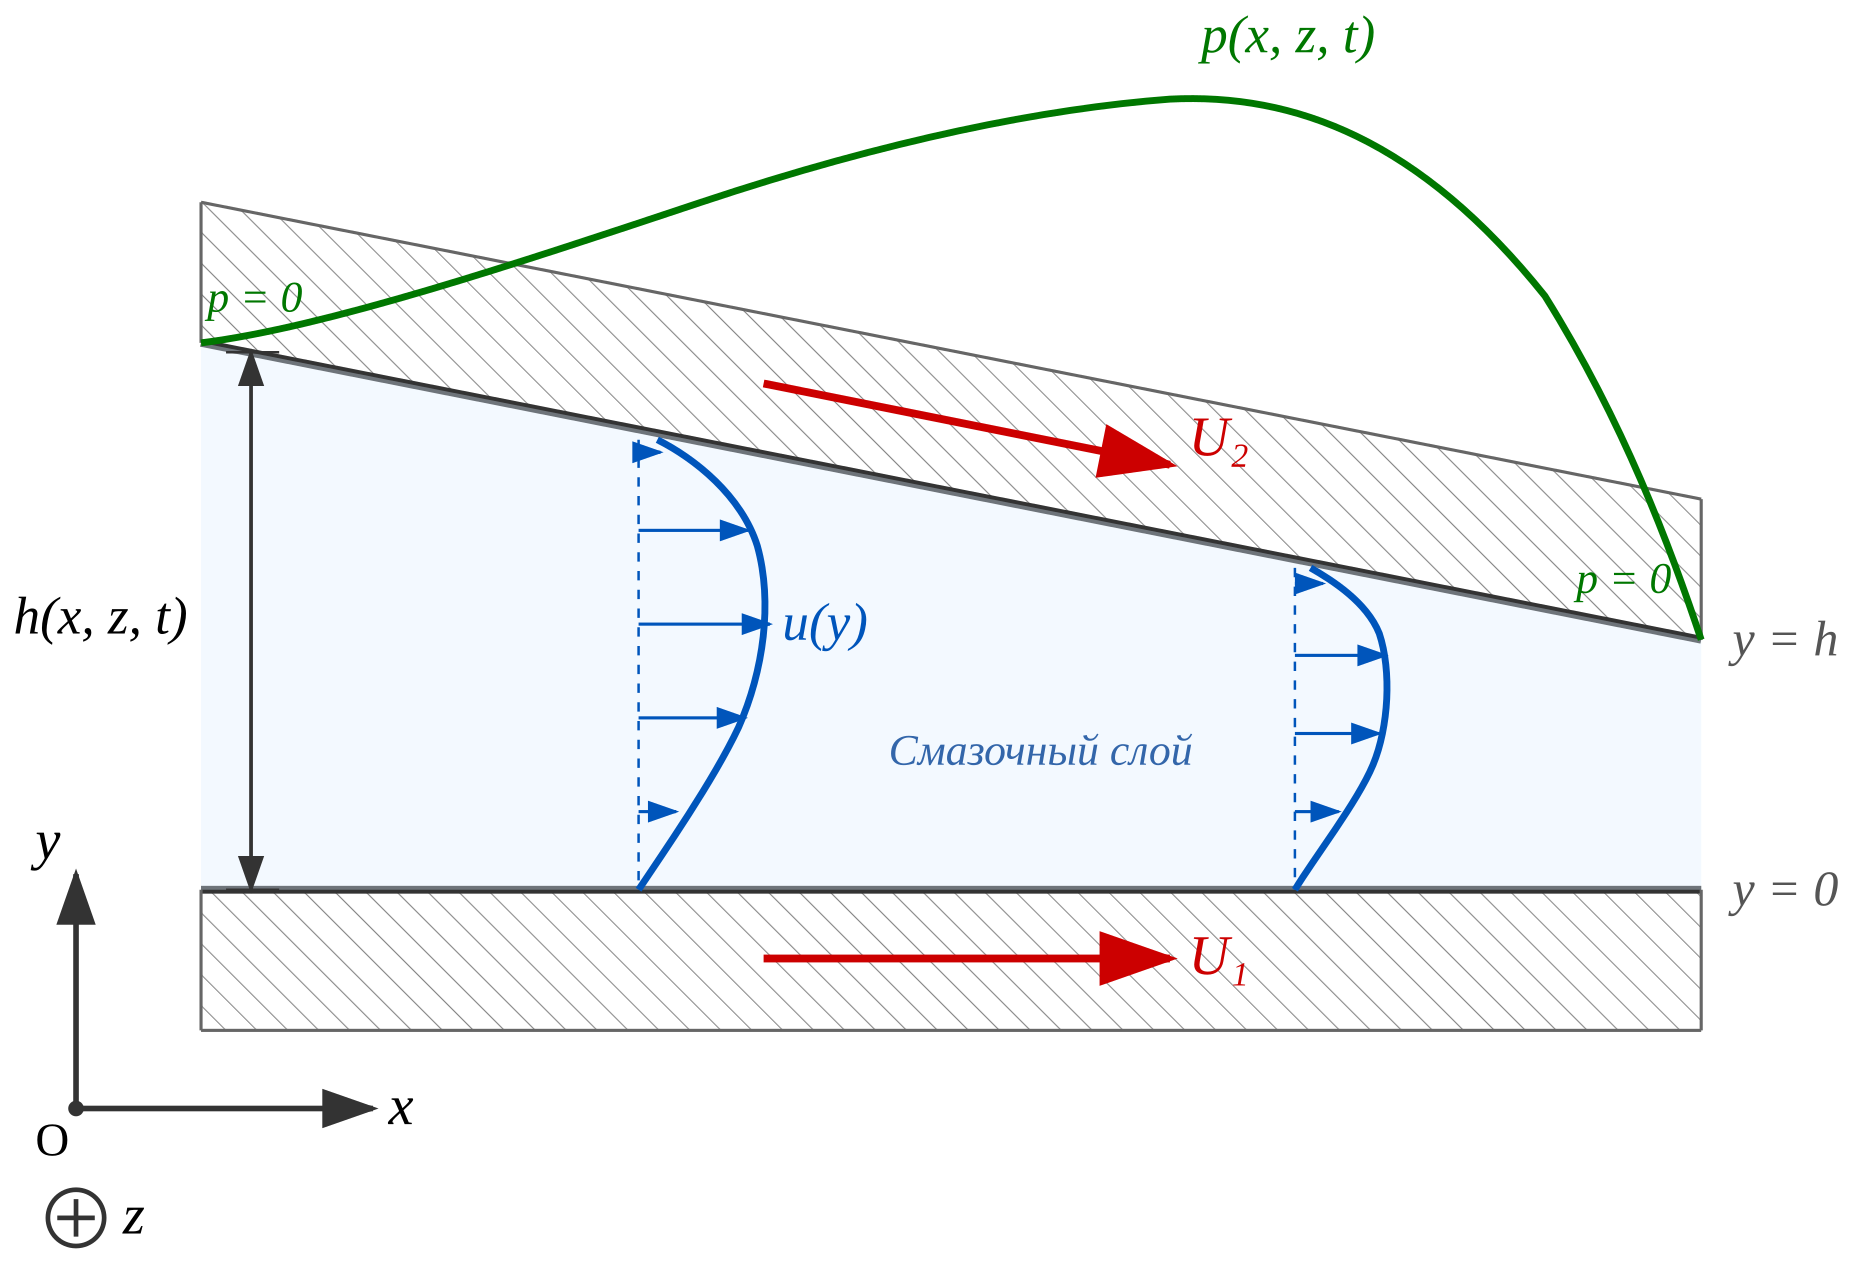
\includegraphics[width=\textwidth,height=0.9\textheight,keepaspectratio]{figures/ch02/fig_2_1.png}
\caption{Схема смазочного слоя между двумя поверхностями}
\label{fig:lubrication_scheme}
\end{figure}

\subsubsection*{Основные допущения}

Вывод уравнения Рейнольдса основан на следующих физических допущениях:

\begin{enumerate}
\item Жидкость ньютоновская: касательные напряжения пропорциональны скоростям деформации, в частности $\tau_{xy} = \mu\,\partial u/\partial y$, $\tau_{yz} = \mu\,\partial w/\partial y$.
\item Жидкость несжимаемая: $\rho = \mathrm{const}$.
\item Тонкий слой: $H \ll L$, где $H$ -- характерный (порядковый) масштаб толщины смазочного слоя $h(x,z,t)$; малые уклоны поверхностей $|\partial h/\partial x| \ll 1$, $|\partial h/\partial z| \ll 1$.
\item Течение ламинарное, инерционные эффекты пренебрежимо малы: $\mathrm{Re}\cdot\epsilon \ll 1$, где $\epsilon = H/L$.
\item Давление постоянно по толщине слоя: $\partial p/\partial y \approx 0$ (следствие смазочной аппроксимации).
\item Динамическая вязкость постоянна: $\mu = \mathrm{const}$ (температурная зависимость рассматривается отдельно при необходимости).
\item На границах жидкости и твёрдых поверхностей выполняется условие прилипания (no-slip).
\item Объёмные силы (гравитация и др.) малы по сравнению с градиентом давления и не учитываются.
\end{enumerate}

\subsubsection*{Исходные уравнения}

Движение жидкости описывается уравнениями Навье--Стокса для несжимаемой жидкости:

\begin{equation}
\rho\left(\frac{\partial \mathbf{v}}{\partial t} + (\mathbf{v} \cdot \nabla)\mathbf{v}\right) = -\nabla p + \mu \nabla^2 \mathbf{v},
\label{eq:navier_stokes}
\end{equation}

и уравнением неразрывности:

\begin{equation}
\nabla \cdot \mathbf{v} = 0,
\label{eq:continuity}
\end{equation}
\begin{conditions}
$\mathbf{v} = (u, v, w)$ -- вектор скорости;\\
$\rho$ -- плотность жидкости;\\
$p$ -- давление;\\
$\mu$ -- динамическая вязкость.
\end{conditions}
В компонентной форме уравнения движения приведены в приложении~А. Уравнение неразрывности~\eqref{eq:continuity} в компонентной записи имеет вид:

\begin{equation}
\frac{\partial u}{\partial x} + \frac{\partial v}{\partial y} + \frac{\partial w}{\partial z} = 0.
\label{eq:continuity_comp}
\end{equation}

Далее, на основе анализа порядков величин, будет получена смазочная аппроксимация и выведено уравнение Рейнольдса.

\subsubsection*{Масштабирование и оценка порядков величин}

Для анализа уравнений введём характерные масштабы задачи:

$L$ -- характерный размер в направлениях $x$ и $z$ (длина подшипника);

$H$ -- характерная толщина смазочного слоя;

$U$ -- характерная скорость движения поверхностей;

$P$ -- характерное давление.

Безразмерные переменные вводятся следующим образом:

\begin{equation}
\bar{x} = \frac{x}{L}, \quad \bar{y} = \frac{y}{H}, \quad \bar{z} = \frac{z}{L}, \quad \bar{u} = \frac{u}{U}, \quad \bar{v} = \frac{v}{V_0}, \quad \bar{w} = \frac{w}{U}, \quad \bar{p} = \frac{p}{P},
\end{equation}
где $V_0$ -- характерная скорость в направлении $y$, которую нужно определить из уравнения неразрывности.

Из уравнения неразрывности следует оценка:

\begin{equation}
\frac{U}{L} \sim \frac{V_0}{H} \quad \Rightarrow \quad V_0 \sim U\frac{H}{L} = U\,\epsilon.
\end{equation}

Ключевым параметром в теории смазки является отношение:

\begin{equation}
\epsilon = \frac{H}{L} \ll 1,
\label{eq:epsilon}
\end{equation}
которое характеризует малость толщины слоя по сравнению с его протяжённостью.

Подставляя безразмерные переменные в компонентные уравнения движения, получаем оценки для различных членов. Из $x$-компоненты уравнения движения при смазочной аппроксимации доминирующий баланс имеет вид:

\begin{equation}
\frac{\partial p}{\partial x} \sim \mu\,\frac{\partial^2 u}{\partial y^2} \quad \Rightarrow \quad \frac{P}{L} \sim \mu\,\frac{U}{H^2} \quad \Rightarrow \quad P \sim \mu\,U\,\frac{L}{H^2}.
\label{eq:pressure_scale}
\end{equation}

Характерное давление определяется балансом вязкого сопротивления потоку в тонком зазоре и продольного градиента давления.

Вводим число Рейнольдса для смазочного слоя:

\begin{equation}
\mathrm{Re} = \frac{\rho U H}{\mu}.
\end{equation}

Отношение инерционных членов к вязким оценивается как:

\begin{equation}
\frac{\rho U^2/L}{P/L} \sim \frac{\rho U^2}{\mu U L/H^2} = \underbrace{\frac{\rho U H}{\mu}}_{\mathrm{Re}}\;\underbrace{\frac{H}{L}}_{\epsilon} = \mathrm{Re}\,\epsilon.
\label{eq:Re_epsilon}
\end{equation}

При условии $\mathrm{Re}\,\epsilon \ll 1$ (что выполняется в большинстве практических случаев) инерционные члены в уравнениях движения пренебрежимо малы по сравнению с вязкими и градиентом давления. Малость этого параметра означает, что инерция жидкости подавлена тонкостью смазочного слоя ($\epsilon = H/L \ll 1$), и течение полностью определяется балансом вязких сил и градиента давления.

Анализируя порядки производных с учётом $\epsilon \ll 1$, получаем:

\begin{equation}
\frac{\partial^2}{\partial y^2} \gg \frac{\partial^2}{\partial x^2}, \quad \frac{\partial^2}{\partial y^2} \gg \frac{\partial^2}{\partial z^2}.
\end{equation}

Таким образом, в $x$- и $z$-компонентах уравнения движения доминируют члены:

\begin{equation}
\frac{\partial p}{\partial x} \sim \mu\frac{\partial^2 u}{\partial y^2}, \quad \frac{\partial p}{\partial z} \sim \mu\frac{\partial^2 w}{\partial y^2}.
\end{equation}

Из $y$-компоненты уравнения движения следует, что величина $\partial p/\partial y$ мала по сравнению с $\partial p/\partial x$ и $\partial p/\partial z$ и имеет порядок $O(\epsilon^2)$, откуда:

\begin{equation}
\frac{\partial p}{\partial y} \approx 0.
\label{eq:dp_dy_zero}
\end{equation}

Это означает, что давление в смазочном слое не зависит от координаты $y$: $p = p(x, z, t)$.

\subsubsection*{Упрощённые уравнения движения}

С учётом сделанных допущений уравнения движения принимают вид:

\begin{equation}
\label{eq:simplified_xz}
\begin{aligned}
\frac{\partial p}{\partial x} &= \mu\frac{\partial^2 u}{\partial y^2}, \\
\frac{\partial p}{\partial z} &= \mu\frac{\partial^2 w}{\partial y^2}.
\end{aligned}
\end{equation}

Уравнение неразрывности сохраняет форму~\eqref{eq:continuity_comp}.

\subsubsection*{Граничные условия}

На поверхностях выполняются условия прилипания (no-slip):

\begin{equation}
\begin{aligned}
&y = 0: \quad u = U_1(x, z, t), \quad w = W_1(x, z, t), \quad v = V_1(x, z, t), \\
&y = h: \quad u = U_2(x, z, t), \quad w = W_2(x, z, t), \quad v = V_2(x, z, t),
\end{aligned}
\label{eq:boundary_conditions}
\end{equation}
где $U_i$, $W_i$, $V_i$ -- компоненты скорости соответствующих поверхностей. В общем случае скорости поверхностей могут зависеть от координат и времени. Далее при выводе уравнения Рейнольдса величины $U_i$ и $W_i$ полагаются постоянными вдоль соответствующей поверхности, что корректно для основных типов подшипников, рассматриваемых в настоящей работе.

\subsubsection*{Профиль скорости}

Интегрируя уравнение~\eqref{eq:simplified_xz} дважды по $y$ и используя граничные условия~\eqref{eq:boundary_conditions}, получаем профиль скорости в направлении $x$:

\begin{equation}
u(x, y, z, t) = U_1 + \frac{y}{h}(U_2 - U_1) + \frac{1}{2\mu}\frac{\partial p}{\partial x}y(y - h).
\label{eq:velocity_profile_u}
\end{equation}

Аналогично для направления $z$:

\begin{equation}
w(x, y, z, t) = W_1 + \frac{y}{h}(W_2 - W_1) + \frac{1}{2\mu}\frac{\partial p}{\partial z}y(y - h).
\label{eq:velocity_profile_w}
\end{equation}

Профиль скорости~\eqref{eq:velocity_profile_u} состоит из двух частей: линейной (куэттовский поток, обусловленный движением поверхностей) и параболической (пуазейлевский поток, обусловленный градиентом давления).

\subsubsection*{Объёмный расход}

Объёмный расход жидкости через единицу длины перпендикулярно направлению $x$ определяется интегрированием скорости по толщине слоя:

\begin{equation}
q_x = \int_0^h u \,\mathrm{d}y.
\end{equation}

Подставляя выражение~\eqref{eq:velocity_profile_u}:

\begin{equation}
q_x = \int_0^h \left[U_1 + \frac{y}{h}(U_2 - U_1) + \frac{1}{2\mu}\frac{\partial p}{\partial x}y(y - h)\right] dy.
\end{equation}

Вычисляем интегралы:

\begin{equation}
\begin{aligned}
&\int_0^h U_1 \,\mathrm{d}y = U_1 h, \\
&\int_0^h \frac{y}{h}(U_2 - U_1) \,\mathrm{d}y = \frac{U_2 - U_1}{h} \cdot \frac{h^2}{2} = \frac{h}{2}(U_2 - U_1), \\
&\int_0^h \frac{1}{2\mu}\frac{\partial p}{\partial x}y(y - h) \,\mathrm{d}y = \frac{1}{2\mu}\frac{\partial p}{\partial x}\left(\frac{h^3}{3} - \frac{h^3}{2}\right) = -\frac{h^3}{12\mu}\frac{\partial p}{\partial x}.
\end{aligned}
\end{equation}

Окончательно для расхода в направлении $x$:

\begin{equation}
q_x = \frac{h}{2}(U_1 + U_2) - \frac{h^3}{12\mu}\frac{\partial p}{\partial x}.
\label{eq:flow_rate_x}
\end{equation}

Аналогично для направления $z$:

\begin{equation}
q_z = \frac{h}{2}(W_1 + W_2) - \frac{h^3}{12\mu}\frac{\partial p}{\partial z}.
\label{eq:flow_rate_z}
\end{equation}

\subsubsection*{Вывод уравнения Рейнольдса}

Из уравнения неразрывности~\eqref{eq:continuity}, интегрируя по толщине слоя от $y = 0$ до $y = h$:

\begin{equation}
\int_0^h \frac{\partial u}{\partial x} \,\mathrm{d}y + \int_0^h \frac{\partial v}{\partial y} \,\mathrm{d}y + \int_0^h \frac{\partial w}{\partial z} \,\mathrm{d}y = 0.
\end{equation}

Используя правило Лейбница для дифференцирования интеграла:

\begin{equation}
\frac{\partial}{\partial x}\int_0^h u \,\mathrm{d}y = \int_0^h \frac{\partial u}{\partial x} \,\mathrm{d}y + u|_{y=h}\frac{\partial h}{\partial x},
\end{equation}
и аналогично для $z$. Таким образом, интегралы производных в уравнении неразрывности выражаются как:

\begin{equation}
\label{eq:leibniz_applied}
\begin{split}
&\int_0^h \frac{\partial u}{\partial x}\,\mathrm{d}y = \frac{\partial}{\partial x}\!\int_0^h u\,\mathrm{d}y
  - u\big|_{y=h}\,\frac{\partial h}{\partial x}, \\
&\int_0^h \frac{\partial w}{\partial z}\,\mathrm{d}y = \frac{\partial}{\partial z}\!\int_0^h w\,\mathrm{d}y
  - w\big|_{y=h}\,\frac{\partial h}{\partial z}.
\end{split}
\end{equation}

Для второго интеграла:

\begin{equation}
\int_0^h \frac{\partial v}{\partial y} \,\mathrm{d}y = v|_{y=h} - v|_{y=0} = V_2 - V_1.
\end{equation}

Кинематическое условие на верхней поверхности $y = h(x,z,t)$:

\begin{equation}
V_2 = \frac{\partial h}{\partial t} + U_2\frac{\partial h}{\partial x} + W_2\frac{\partial h}{\partial z}.
\label{eq:kinematic_upper}
\end{equation}

Нижняя поверхность полагается плоской и неподвижной в направлении $y$, откуда $V_1 = 0$. Здесь использовано условие прилипания на верхней поверхности: $u(h) = U_2$, $w(h) = W_2$, $v(h) = V_2$. Подставляя~\eqref{eq:leibniz_applied} и кинематическое условие~\eqref{eq:kinematic_upper} в интегрированное уравнение неразрывности, после сокращения членов $U_2\,\partial h/\partial x$ и $W_2\,\partial h/\partial z$, приходим к уравнению:

Используя определения расходов~\eqref{eq:flow_rate_x} и~\eqref{eq:flow_rate_z}:

\begin{equation}
\frac{\partial q_x}{\partial x} + \frac{\partial q_z}{\partial z} + \frac{\partial h}{\partial t} = 0.
\label{eq:continuity_integrated}
\end{equation}

Уравнение~\eqref{eq:continuity_integrated} допускает наглядную интерпретацию в терминах контрольного объёма (рисунок~\ref{fig:control_volume}): изменение толщины слоя $\partial h/\partial t$ компенсируется потоками $q_x$ и $q_z$ через боковые грани элемента $dx \times dz$.

% [РИСУНОК: Контрольный объём смазочного слоя]
% Должен показывать:
% - Элемент dx × dz, толщина h
% - Потоки q_x и q_x + ∂q_x/∂x·dx через левую и правую грани
% - Потоки q_z и q_z + ∂q_z/∂z·dz через переднюю и заднюю грани
% - Стрелка ∂h/∂t сверху (выжимание)
% - Формула баланса: ∂q_x/∂x + ∂q_z/∂z + ∂h/∂t = 0
\begin{figure}[!ht]
\centering
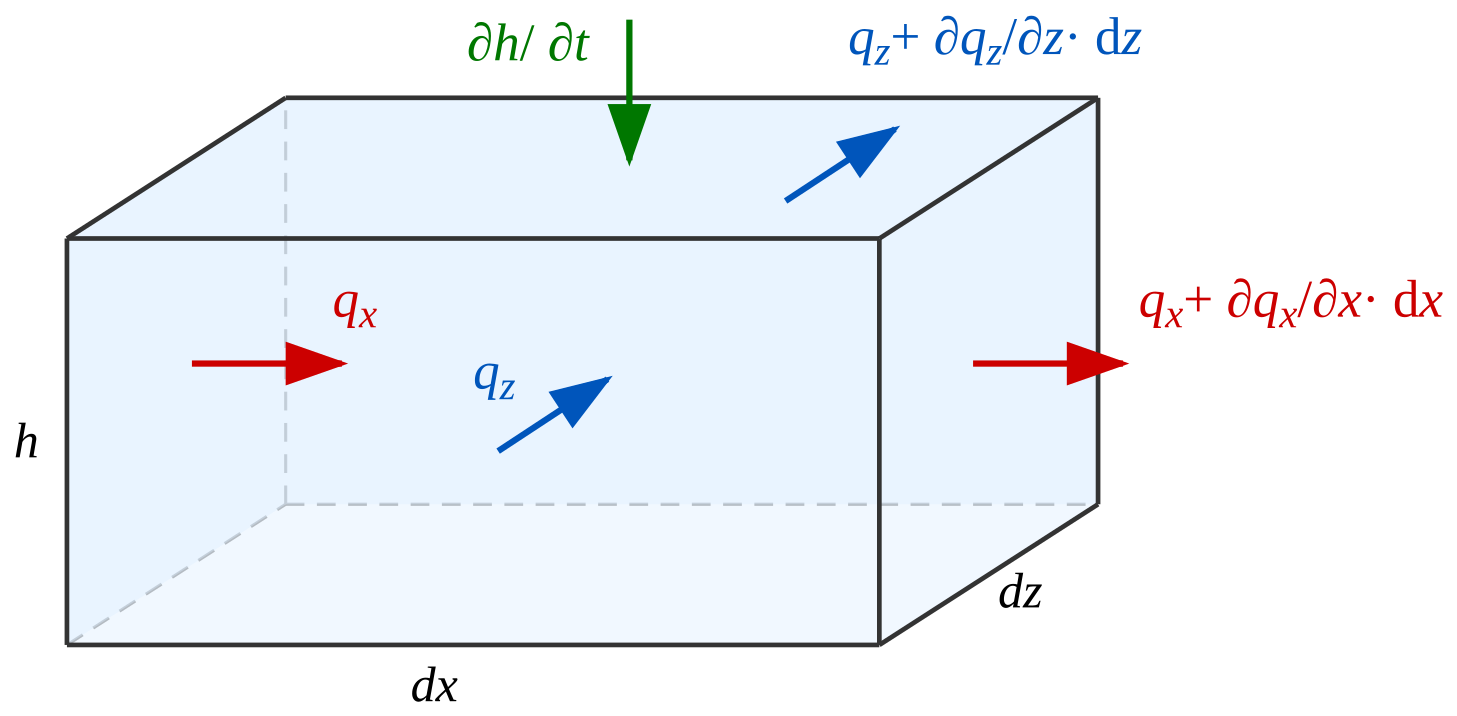
\includegraphics[width=\textwidth,height=0.9\textheight,keepaspectratio]{figures/ch02/fig_2_2.png}
\caption{Контрольный объём смазочного слоя и баланс расходов}
\label{fig:control_volume}
\end{figure}

\FloatBarrier

Подставляя выражения для $q_x$ и $q_z$:

\begin{equation}
\begin{split}
&\frac{\partial}{\partial x}\left[\frac{h}{2}(U_1 + U_2) - \frac{h^3}{12\mu}\frac{\partial p}{\partial x}\right] + {} \\
&+ \frac{\partial}{\partial z}\left[\frac{h}{2}(W_1 + W_2) - \frac{h^3}{12\mu}\frac{\partial p}{\partial z}\right] + \frac{\partial h}{\partial t} = 0.
\end{split}
\end{equation}

Раскрывая производные:

\begin{equation}
\label{eq:reynolds_full}
\begin{split}
&\frac{\partial}{\partial x}\left(\frac{h^3}{12\mu}\frac{\partial p}{\partial x}\right) + \frac{\partial}{\partial z}\left(\frac{h^3}{12\mu}\frac{\partial p}{\partial z}\right) = {} \\
&= \frac{\partial}{\partial x}\left[\frac{h}{2}(U_1 + U_2)\right] + \frac{\partial}{\partial z}\left[\frac{h}{2}(W_1 + W_2)\right] + \frac{\partial h}{\partial t}.
\end{split}
\end{equation}

Уравнение~\eqref{eq:reynolds_full} является \textbf{обобщённым уравнением Рейнольдса} для случая нестационарного течения с подвижными границами произвольной формы.
Вязкость~$\mu$ записана под знаком производных, что обеспечивает корректность формулы и при переменной вязкости $\mu = \mu(x, z)$ (например, при учёте температурной зависимости в главе~4).

Для стационарного случая ($\partial h/\partial t = 0$) и при условии $W_1 = W_2 = 0$ (движение только в направлении $x$) уравнение упрощается:

\begin{equation}
\frac{\partial}{\partial x}\left(\frac{h^3}{12\mu}\frac{\partial p}{\partial x}\right) + \frac{\partial}{\partial z}\left(\frac{h^3}{12\mu}\frac{\partial p}{\partial z}\right) = \frac{U_1 + U_2}{2}\frac{\partial h}{\partial x}.
\label{eq:reynolds_steady}
\end{equation}

Уравнение~\eqref{eq:reynolds_steady} представляет собой \textbf{классическое уравнение Рейнольдса} для гидродинамической смазки.

В случае одной движущейся поверхности (например, $U_1 = U$, $U_2 = 0$) и постоянной вязкости $\mu = \mathrm{const}$ обе части уравнения можно умножить на~$12\mu$, что даёт эквивалентную форму, удобную для численной реализации:

\begin{equation}
\frac{\partial}{\partial x}\left(h^3\frac{\partial p}{\partial x}\right) + \frac{\partial}{\partial z}\left(h^3\frac{\partial p}{\partial z}\right) = 6\mu\,U\frac{\partial h}{\partial x}.
\label{eq:reynolds_one_surface}
\end{equation}

Полученное уравнение Рейнольдса~\eqref{eq:reynolds_one_surface} является основным уравнением теории гидродинамической смазки и связывает распределение давления $p(x, z)$ в смазочном слое с геометрией зазора $h(x, z)$ и скоростью движения поверхности $U$~\cite{hori2002,szeri1998}.

Следует отметить, что при решении уравнения Рейнольдса в областях расходящегося зазора могут возникать зоны отрицательного давления, не имеющие физического смысла. Для корректного описания таких областей необходима массо-сохраняющая модель кавитации, которая рассматривается в разделе~2.3 на основе подхода Jakobsson--Floberg--Olsson (JFO).

\FloatBarrier
\subsection{Постановка задачи для торцевого зазора}

% Упорный подшипник (thrust bearing)
% Полная постановка задачи: геометрия, кинематика, уравнение Рейнольдса,
% граничные условия, расходы, целевые функционалы

Рассмотрим упорный (осевой) подшипник скольжения -- узел, в котором осевая нагрузка воспринимается тонким слоем вязкой жидкости, заключённым между двумя поверхностями: вращающимся диском (ротором) и неподвижной опорной поверхностью (колодкой, или сектором). Несущая способность подшипника обусловлена гидродинамическим давлением, которое генерируется в сходящемся зазоре при относительном движении поверхностей.

Упорные подшипники скольжения находят широкое применение в инженерной практике. В турбинах гидро- и теплоэнергетических установок они воспринимают осевое усилие, создаваемое рабочим телом на рабочем колесе. В центробежных насосах и компрессорах упорные подшипники фиксируют осевое положение ротора, предотвращая контакт вращающихся и неподвижных элементов. В тяжёлых прокатных станах и вертикальных гидрогенераторах упорные подшипники несут вес ротора и всего рабочего оборудования~\cite{hori2002,szeri1998}.

Цель постановки: для заданной геометрии зазора $h(r,\theta)$ и режима движения поверхностей получить распределение давления $p(r,\theta)$ в смазочном слое. По найденному полю давления далее вычисляются интегральные характеристики, приведённые в подразделе~2.1.7. Все допущения, принятые при выводе уравнения Рейнольдса в подразделе~2.1.1, сохраняют силу: жидкость ньютоновская и несжимаемая, течение ламинарное и стационарное, давление постоянно по толщине смазочного слоя. Далее рассматривается один сектор (колодка) подшипника; полный подшипник состоит из $N$ одинаковых секторов, расположенных равномерно по окружности.


\subsubsection*{Геометрия и система координат}

Для описания упорного подшипника естественно использовать цилиндрические координаты $(r, \theta, y)$:
\begin{itemize}
\item $r$ -- радиальная координата в плоскости подшипника;
\item $\theta$ -- окружная координата, отсчитываемая по направлению вращения;
\item $y$ -- координата по толщине смазочного слоя, направленная перпендикулярно рабочим поверхностям (от $y = 0$ на неподвижной колодке до $y = h$ на вращающемся диске).
\end{itemize}

Область расчёта для одного сектора определяется следующим образом:
\begin{equation}
r \in [R_{\mathrm{in}},\; R_{\mathrm{out}}], \quad \theta \in [\theta_0,\; \theta_1],
\label{eq:thrust_domain}
\end{equation}
\begin{conditions}
$R_{\mathrm{in}}$ и $R_{\mathrm{out}}$ -- внутренний и наружный радиусы рабочей зоны подшипника;\\
$\theta_0$ и $\theta_1$ -- угловые границы сектора.
\end{conditions}
Угловая протяжённость сектора обозначается
\begin{equation}
\beta = \theta_1 - \theta_0.
\label{eq:thrust_beta}
\end{equation}

Граница $\theta_0$ соответствует входной кромке (leading edge), а $\theta_1$ -- выходной кромке (trailing edge) по направлению вращения диска. Толщина смазочного слоя в каждой точке расчётной области составляет $y \in [0,\; h(r,\theta)]$.

Для подшипника из $N$ одинаковых секторов, расположенных равномерно по окружности, угловая протяжённость одного сектора определяется как $\beta = 2\pi/N$ за вычетом углового зазора между соседними колодками. Расчётная область одного сектора схематически изображена на рисунке~\ref{fig:thrust_bearing}.

% [РИСУНОК: Схема упорного подшипника — вид сверху на сектор]
% Должен показывать:
% - Вид сверху на один сектор подшипника
% - Оси r, θ, направление вращения ω
% - Границы R_in, R_out, θ_0, θ_1
% - Угловую протяжённость β
\begin{figure}[!ht]
\centering
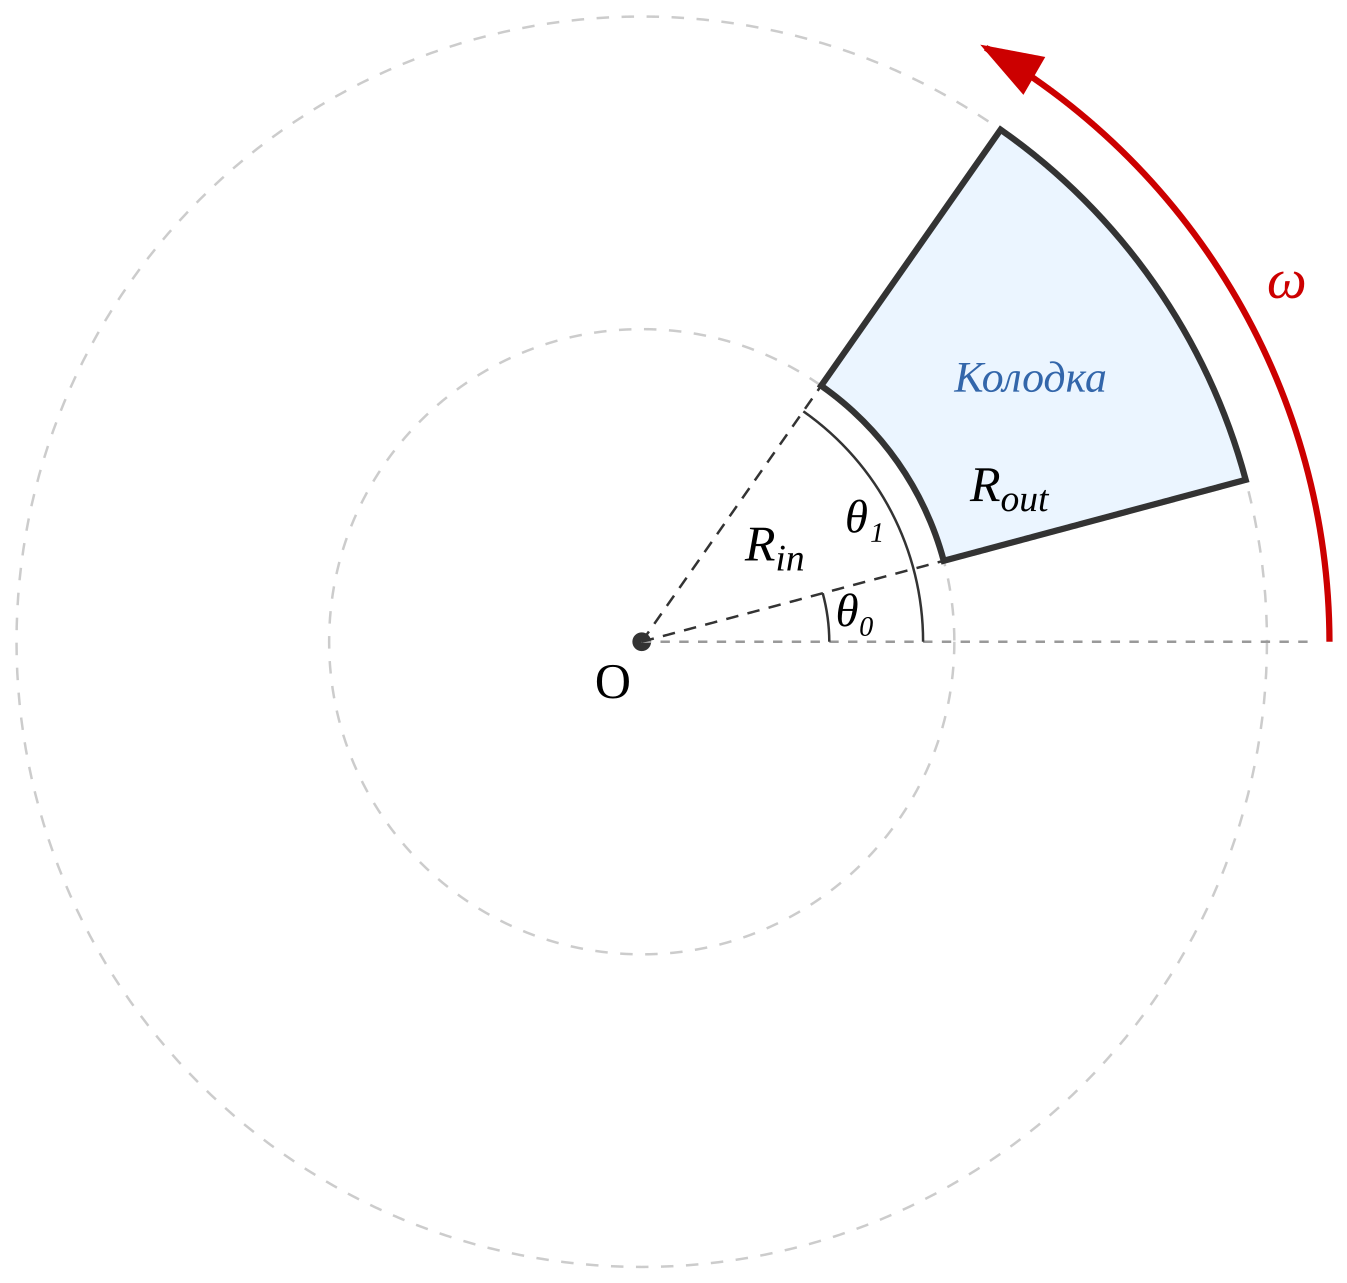
\includegraphics[width=\textwidth,height=0.9\textheight,keepaspectratio]{figures/ch02/fig_2_3.png}
\caption{Схема упорного подшипника: вид сверху на один сектор}
\label{fig:thrust_bearing}
\end{figure}


\subsubsection*{Кинематика движения поверхностей}

Нижняя поверхность ($y = 0$) представляет собой неподвижную колодку, верхняя поверхность ($y = h$) -- вращающийся диск с постоянной угловой скоростью $\omega$. Тангенциальная (окружная) скорость скольжения вращающегося диска в точке с радиальной координатой $r$ составляет:
\begin{equation}
U_\theta(r) = \omega\,r.
\label{eq:thrust_U_theta}
\end{equation}

Радиальные скорости обеих поверхностей равны нулю: $U_{r,1} = U_{r,2} = 0$. В стационарном режиме нормальные скорости поверхностей также обращаются в нуль: $V_1 = V_2 = 0$, что исключает эффект выжимания ($\partial h/\partial t = 0$).

Динамическая вязкость смазки полагается постоянной: $\mu = \mathrm{const}$ (допущение~6 из подраздела~2.1.1). Влияние температурной зависимости вязкости $\mu(T)$ на характеристики подшипника рассматривается отдельно в главе~4.

Вращение диска создаёт тангенциальный увлекающий поток (куэттовскую составляющую течения): жидкость, увлекаемая подвижной поверхностью за счёт условия прилипания, движется в окружном направлении. Когда такой поток проходит через участок зазора с уменьшающейся толщиной, условие неразрывности (сохранения массы) приводит к росту давления в смазочном слое -- именно этот механизм, называемый клиновым эффектом, обеспечивает несущую способность подшипника.


\subsubsection*{Закон толщины смазочного слоя}

В общем случае толщина смазочного слоя является заданной функцией координат:
\begin{equation}
h = h(r, \theta),
\label{eq:thrust_h_general}
\end{equation}
определяющей профиль зазора между колодкой и вращающимся диском. В разделе~2.2 функция $h(r,\theta)$ будет расширена для учёта детерминированных микроструктур рабочей поверхности.

Для тестирования численных методов и верификации результатов широко используется базовая геометрия -- линейный клин, в котором толщина зазора линейно изменяется по окружной координате:
\begin{equation}
h(r,\theta) = h_{\mathrm{in}} + (h_{\mathrm{out}} - h_{\mathrm{in}})\,\frac{\theta - \theta_0}{\theta_1 - \theta_0},
\label{eq:thrust_h_wedge}
\end{equation}
\begin{conditions}
$h_{\mathrm{in}} = h(\theta_0)$ -- толщина смазочного слоя на входной кромке сектора;\\
$h_{\mathrm{out}} = h(\theta_1)$ -- толщина на выходной кромке.
\end{conditions}
Необходимым условием генерации давления является сходящийся характер зазора по направлению движения, т.\,е.
\begin{equation}
h_{\mathrm{in}} > h_{\mathrm{out}}.
\label{eq:thrust_convergence_condition}
\end{equation}

В частном случае $h_{\mathrm{in}} = h_{\mathrm{out}}$ (плоскопараллельный зазор) правая часть уравнения Рейнольдса обращается в нуль и давление не генерируется.

В формуле~\eqref{eq:thrust_h_wedge} величины $h_{\mathrm{in}}$ и $h_{\mathrm{out}}$ приняты постоянными по радиальной координате $r$, что соответствует плоскому клину. Минимальная толщина смазочного слоя обозначается
\begin{equation}
h_{\min} = \min_{(r,\theta)} h(r,\theta);
\label{eq:thrust_h_min}
\end{equation}
для линейного клина $h_{\min} = h_{\mathrm{out}}$.

Для характеристики формы клина вводятся безразмерные параметры конвергенции:
\begin{equation}
K = \frac{h_{\mathrm{in}}}{h_{\mathrm{out}}}, \quad \delta = \frac{h_{\mathrm{in}} - h_{\mathrm{out}}}{h_{\mathrm{out}}} = K - 1.
\label{eq:thrust_convergence}
\end{equation}

При $K = 1$ ($\delta = 0$) зазор является плоскопараллельным и давление не генерируется. Оптимальное значение параметра $K$, обеспечивающее максимальную несущую способность, зависит от соотношения размеров подшипника и определяется численно.

Помимо линейного клина, на практике применяются более сложные профили зазора: ступенчатый (профиль Рэлея), параболический, составной (с плоским участком и клиновой частью). Все перечисленные варианты описываются тем же уравнением Рейнольдса при соответствующем задании функции $h(r,\theta)$. Линейный клин~\eqref{eq:thrust_h_wedge} используется в настоящей работе как базовый верификационный профиль; в реальной колодке профиль зазора $h(r,\theta)$ определяется наклоном опоры и формой рабочей поверхности, что может приводить к зависимости $h$ от радиальной координаты~$r$. Продольное сечение клинового зазора при фиксированном $r$ аналогично общей схеме смазочного слоя (рисунок~\ref{fig:lubrication_scheme}), где горизонтальная координата~$x$ заменяется на~$\theta$, нижняя поверхность соответствует неподвижной колодке, а верхняя~-- плоскому вращающемуся диску со скоростью~$U_\theta = \omega r$. Зазор сужается от~$h_{\mathrm{in}}$ на входном крае колодки до~$h_{\mathrm{out}}$ на выходном.



\subsubsection*{Уравнение Рейнольдса в цилиндрических координатах}

Обобщённое уравнение Рейнольдса~\eqref{eq:reynolds_full}, полученное в подразделе~2.1.1 в декартовых координатах, необходимо переписать в цилиндрических координатах $(r, \theta)$, естественных для задачи об упорном подшипнике. Переход осуществляется введением дуговой координаты $s = r\theta$, вдоль которой производная принимает вид $\partial/\partial s = (1/r)\,\partial/\partial\theta$. Оператор дивергенции и градиента в плоскости $(r, \theta)$ приобретает стандартные множители $1/r$ и $1/r^2$, присутствующие в левой части уравнения Рейнольдса.

В рассматриваемой задаче скорость скольжения направлена по окружной координате~$\theta$: нижняя поверхность неподвижна ($U_{\theta,1} = 0$), верхняя движется со скоростью $U_{\theta,2} = \omega r$; радиальные скорости обеих поверхностей равны нулю. Правая часть обобщённого уравнения Рейнольдса~\eqref{eq:reynolds_full} в цилиндрических координатах записывается в дивергентной форме:
\begin{equation}
\mathrm{RHS} = \frac{1}{r}\frac{\partial}{\partial\theta}\!\left[\frac{h}{2}
(U_{\theta,1} + U_{\theta,2})\right], \quad U_{\theta,1} = 0,\quad U_{\theta,2} = \omega r,
\label{eq:thrust_rhs_div}
\end{equation}
откуда, учитывая, что произведение $\omega r$ не зависит от~$\theta$:
\begin{equation}
\frac{U_{\theta,1} + U_{\theta,2}}{2}\,\frac{1}{r}\,\frac{\partial h}{\partial \theta} = \frac{\omega r}{2}\,\frac{1}{r}\,\frac{\partial h}{\partial \theta} = \frac{\omega}{2}\,\frac{\partial h}{\partial \theta}.
\label{eq:thrust_rhs_derivation}
\end{equation}

Стационарное уравнение Рейнольдса для несжимаемой ньютоновской жидкости в цилиндрических координатах принимает вид:
\begin{equation}
\label{eq:thrust_reynolds}
\frac{1}{r}\frac{\partial}{\partial r}\!\left[r\,\frac{h^3}{12\mu}\,\frac{\partial p}{\partial r}\right] + \frac{1}{r^2}\frac{\partial}{\partial \theta}\!\left[\frac{h^3}{12\mu}\,\frac{\partial p}{\partial \theta}\right] = \frac{\omega}{2}\,\frac{\partial h}{\partial \theta}.
\end{equation}

Множители $1/r$ и $1/r^2$ перед производными в левой части обусловлены дивергентной формой эллиптического оператора $\nabla \cdot (h^3 \nabla p)$ в цилиндрических координатах. Оператор Лапласа является его частным случаем при $h = \mathrm{const}$.

Умножая обе части уравнения~\eqref{eq:thrust_reynolds} на~$12\mu$ (что допустимо при $\mu = \mathrm{const}$), получаем эквивалентную форму, удобную для численной реализации:
\begin{equation}
\frac{1}{r}\frac{\partial}{\partial r}\!\left[r\,h^3\,\frac{\partial p}{\partial r}\right] + \frac{1}{r^2}\frac{\partial}{\partial \theta}\!\left[h^3\,\frac{\partial p}{\partial \theta}\right] = 6\mu\omega\,\frac{\partial h}{\partial \theta}.
\label{eq:thrust_reynolds_num}
\end{equation}

Уравнение~\eqref{eq:thrust_reynolds_num} является основным расчётным уравнением для упорного подшипника в настоящей работе.

Левая часть уравнений~\eqref{eq:thrust_reynolds}-\eqref{eq:thrust_reynolds_num} представляет собой эллиптический оператор, описывающий перераспределение давления через вязкий смазочный слой: давление <<диффундирует>> как в радиальном, так и в окружном направлениях, причём <<проводимость>> пропорциональна кубу толщины зазора~$h^3$. Правая часть -- источниковый член, обусловленный изменением толщины зазора в направлении движения (клиновой эффект). При $\partial h/\partial \theta = 0$ (плоскопараллельный зазор) правая часть обращается в нуль, и при однородных граничных условиях уравнение допускает лишь тривиальное решение $p = 0$ -- давление не генерируется.

При наличии детерминированных микроструктур на рабочей поверхности функция $h(r,\theta)$ приобретает быстрые локальные вариации. Формально уравнение~\eqref{eq:thrust_reynolds_num} остаётся тем же, однако функция зазора существенно усложняется, что описывается в разделе~2.2.


\subsubsection*{Граничные условия}

Для замыкания уравнения Рейнольдса~\eqref{eq:thrust_reynolds_num} необходимо задать граничные условия на давление по всему контуру расчётной области~\eqref{eq:thrust_domain}. Рассмотрим три практически важных варианта.

\textit{Базовый вариант (атмосферные кромки).} На всех четырёх границах сектора давление принимается равным атмосферному:
\begin{equation}
\begin{aligned}
&p(r,\,\theta_0) = 0, \quad p(r,\,\theta_1) = 0, \\
&p(R_{\mathrm{in}},\,\theta) = 0, \quad p(R_{\mathrm{out}},\,\theta) = 0.
\end{aligned}
\label{eq:thrust_bc_base}
\end{equation}

Здесь давление отсчитывается от атмосферного ($p = p_{\mathrm{abs}} - p_{\mathrm{atm}}$). Условие~\eqref{eq:thrust_bc_base} соответствует изолированному сектору, кромки которого свободно сообщаются с окружающей средой, а принудительная подача смазки отсутствует. Данный вариант является наиболее распространённым при расчёте несамоустанавливающихся колодок.

\textit{Вариант с давлением подачи.} Если система смазки обеспечивает принудительную подачу жидкости через входную кромку сектора, граничное условие на $\theta = \theta_0$ модифицируется:
\begin{equation}
p(r,\,\theta_0) = p_{\mathrm{sup}}(r),
\label{eq:thrust_bc_supply}
\end{equation}
где $p_{\mathrm{sup}}(r)$ -- заданное давление подачи смазки; в простейшем случае $p_{\mathrm{sup}} = \mathrm{const}$. Остальные граничные условия остаются такими же, как в базовом варианте~\eqref{eq:thrust_bc_base}. Величина $p_{\mathrm{sup}}$ определяется конструкцией системы смазки и режимом работы насоса подачи.

\textit{Кавитация.} При решении уравнения Рейнольдса в областях расходящегося зазора расчётное давление может оказаться отрицательным. Отрицательное давление физически не реализуется: при снижении давления ниже давления насыщенных паров смазки жидкость разрывается и образуется кавитационная зона с парогазовой смесью. В простейшей постановке применяют ограничение $p \geq 0$ (условие Гюмбеля), при котором отрицательные давления обнуляются после решения. Такой подход, однако, нарушает закон сохранения массы на границе кавитационной зоны. Корректная массо-сохраняющая постановка, основанная на модели Jakobsson--Floberg--Olsson (JFO), вводится в разделе~2.3. Граница между зоной полного смазочного слоя и кавитационной зоной заранее неизвестна и определяется в процессе решения как часть задачи.

Следует отметить, что условия Дирихле $p = 0$ на всех четырёх границах сектора представляют лишь один из возможных вариантов замыкания задачи. В зависимости от конструкции узла и схемы смазки могут применяться и другие постановки: периодичность по $\theta$ (при моделировании полного кольцевого сегмента без разрывов), условие непротекания через радиальные границы $q_r = 0$, что эквивалентно $\partial p/\partial r = 0$ (при наличии уплотнений или перемычек), а также смешанные условия при комбинированной подаче смазки. Конкретный набор граничных условий определяется конструкцией узла и схемой подвода смазки.

Перечисленные варианты граничных условий схематически показаны на рисунке~\ref{fig:thrust_bc_schemes}.

% [РИСУНОК: Варианты граничных условий на секторе]
% Должен показывать три подрисунка (a), (b), (c):
% (a) Базовый: p = 0 на всех 4 границах сектора
% (b) С подпиткой: p = p_sup на θ = θ_0, остальные p = 0
% (c) Альтернативный: ∂p/∂r = 0 на радиальных границах (уплотнения)
%     или периодичность по θ
% На каждом подрисунке — контур сектора с обозначением ГУ на каждой стороне
\begin{figure}[!ht]
\centering
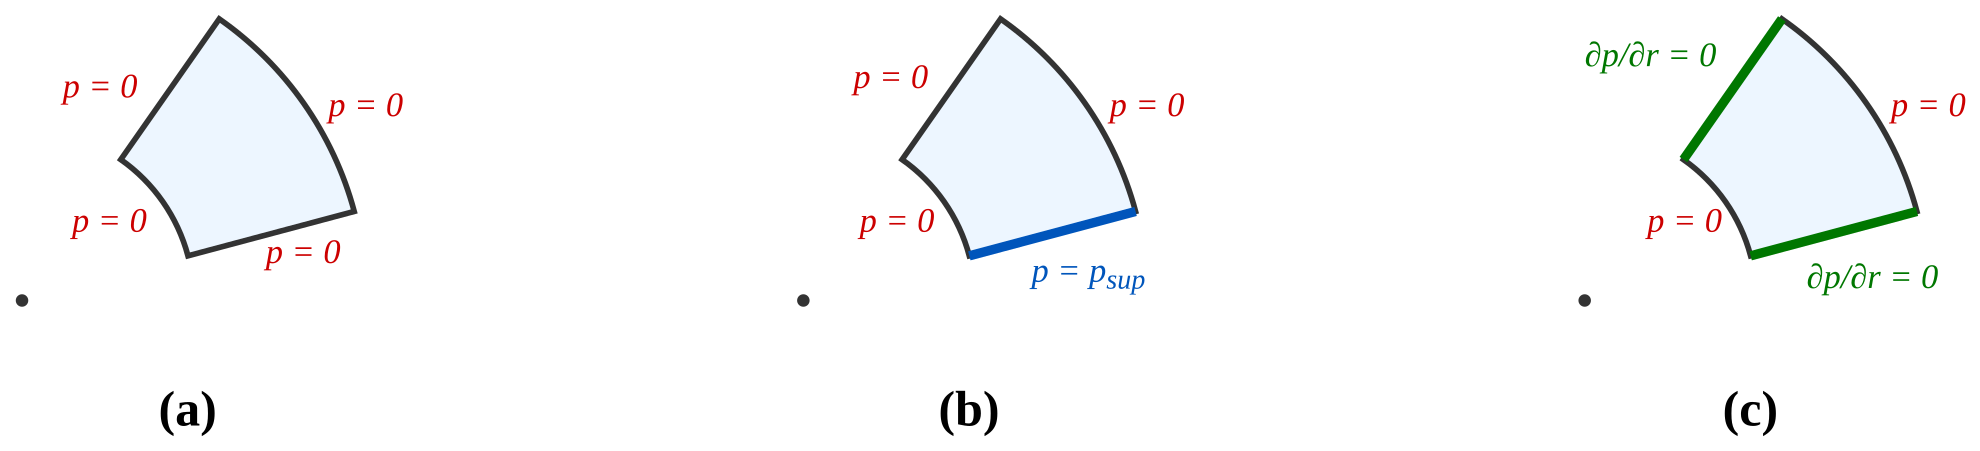
\includegraphics[width=\textwidth,height=0.9\textheight,keepaspectratio]{figures/ch02/fig_2_4.png}
\caption{Варианты граничных условий для упорного подшипника: (a)~$p=0$ на всех четырёх границах сектора (атмосферные кромки); (b)~$p=p_{\mathrm{sup}}$ на входной кромке $\theta=\theta_0$ (принудительная подача), остальные границы $p=0$; (c)~$\partial p/\partial r=0$ на радиальных границах (уплотнения), $p=0$ на дуговых кромках}
\label{fig:thrust_bc_schemes}
\end{figure}

\begin{figure}[!ht]
\centering
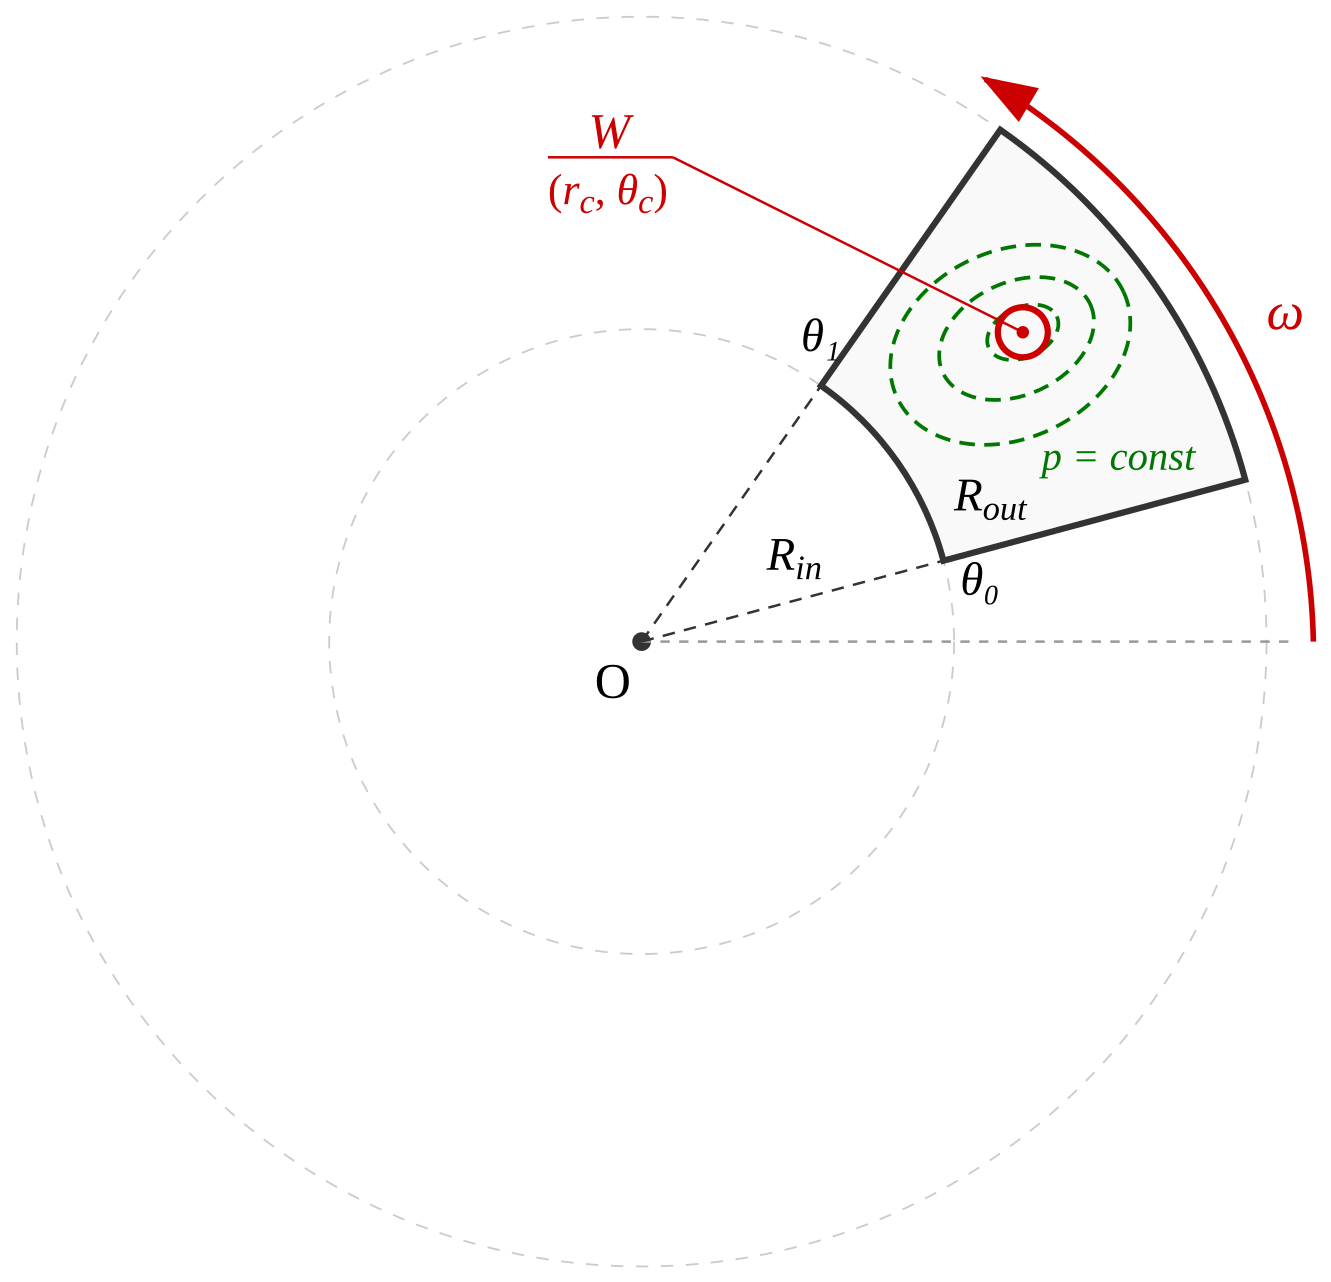
\includegraphics[width=\textwidth,height=0.9\textheight,keepaspectratio]{figures/ch02/fig_2_5.png}
\caption{Результирующая сила~$W$ и изобары давления на секторе упорного подшипника;
  $(r_c,\,\theta_c)$~--- координаты центра давления}
\label{fig:thrust_pressure_map}
\end{figure}


\subsubsection*{Объёмные расходы}

Объёмные расходы жидкости через единицу длины определяются путём интегрирования профилей скорости по толщине смазочного слоя, аналогично выражениям~\eqref{eq:flow_rate_x}-\eqref{eq:flow_rate_z}, полученным в подразделе~2.1.1 в декартовых координатах. Ниже приведены формулы, адаптированные к цилиндрической системе координат.

Радиальный расход (на единицу длины по окружной координате):
\begin{equation}
q_r(r,\theta) = -\frac{h^3}{12\mu}\,\frac{\partial p}{\partial r}.
\label{eq:thrust_q_r}
\end{equation}

Поскольку радиальные скорости обеих поверхностей равны нулю, куэттовская составляющая в радиальном направлении отсутствует. Радиальный расход полностью определяется градиентом давления (пуазейлевская составляющая).

Окружной расход (на единицу длины по радиальной координате):
\begin{equation}
q_\theta(r,\theta) = \frac{h\,\omega\,r}{2} - \frac{h^3}{12\mu\,r}\,\frac{\partial p}{\partial \theta}.
\label{eq:thrust_q_theta}
\end{equation}

Первое слагаемое в~\eqref{eq:thrust_q_theta} представляет куэттовскую составляющую расхода, обусловленную увлечением жидкости вращающейся поверхностью. При $U_{\theta,1}=0$ и $U_{\theta,2}=\omega r$ средняя скорость потока составляет $\bar{U}_\theta = \omega r / 2$, а объёмный расход через единицу длины равен $h\,\bar{U}_\theta = h\omega r/2$. Второе слагаемое -- пуазейлевская составляющая; множитель $1/r$ в знаменателе возникает из-за метрического коэффициента при переходе от производной по дуге $\partial/\partial(r\theta)$ к производной по углу $\partial/\partial\theta$.

Суммарные объёмные расходы через радиальные границы подшипника получаются интегрированием удельных расходов по окружной кромке:
\begin{equation}
\label{eq:thrust_Q_radial}
\begin{split}
&Q_{\mathrm{out}} = \int_{\theta_0}^{\theta_1} q_r(R_{\mathrm{out}}, \theta)\,R_{\mathrm{out}}\,\mathrm{d}\theta, \\
&Q_{\mathrm{in}} = \int_{\theta_0}^{\theta_1} q_r(R_{\mathrm{in}}, \theta)\,R_{\mathrm{in}}\,\mathrm{d}\theta.
\end{split}
\end{equation}

Множитель $R_{\mathrm{out}}$ (соответственно, $R_{\mathrm{in}}$) перед $d\theta$ обусловлен элементом длины дуги $dl = r\,\mathrm{d}\theta$ на окружности радиуса $r$.

Разность $Q_{\mathrm{out}} - Q_{\mathrm{in}}$ определяет утечку смазки через радиальные кромки сектора. Суммарный окружной расход через входную и выходную окружные кромки дополняет баланс массы: полный расход жидкости, поступающей в сектор, равен полному расходу, покидающему его.

Баланс массы в стационарном режиме без выжимания записывается в дифференциальной форме:
\begin{equation}
\frac{1}{r}\,\frac{\partial (r\,q_r)}{\partial r} + \frac{1}{r}\,\frac{\partial q_\theta}{\partial \theta} = 0.
\label{eq:thrust_mass_balance}
\end{equation}

Подстановка выражений~\eqref{eq:thrust_q_r} и~\eqref{eq:thrust_q_theta} в уравнение~\eqref{eq:thrust_mass_balance} приводит к уравнению Рейнольдса~\eqref{eq:thrust_reynolds}, что подтверждает внутреннюю согласованность полученных соотношений.


Решение уравнения Рейнольдса даёт поле давления~$p$ в расчётной области. По найденному давлению вычисляются интегральные характеристики узла: несущая способность, расходы смазки, силы и моменты трения, минимальная толщина плёнки~\cite{majumdar2004}. Унифицированные формулы для всех выходных величин приведены в подразделе~2.1.7.

Сформулированная задача сводится к решению эллиптического уравнения Рейнольдса~\eqref{eq:thrust_reynolds_num} в области~\eqref{eq:thrust_domain} при заданном профиле зазора $h(r,\theta)$ и граничных условиях на давление. Структура уравнения (эллиптический оператор в левой части, источниковый член в правой) обеспечивает единственность решения при корректно поставленных граничных условиях Дирихле в отсутствие кавитации, т.\,е. для линейной постановки без ограничений на знак давления.

Численная дискретизация уравнения~\eqref{eq:thrust_reynolds_num} методом конечных разностей и алгоритм учёта кавитации на основе модели JFO рассматриваются в главе~3. При наличии микроструктур на рабочей поверхности функция зазора $h(r,\theta)$ приобретает быстрые локальные вариации, параметризация которых описывается в разделе~2.2.

\FloatBarrier
\subsection{Постановка задачи для радиального зазора при окружном сдвиге}

% Радиальный подшипник (journal bearing)

Рассмотрим радиальный (опорный) подшипник скольжения -- узел, в котором цилиндрический вал (цапфа) вращается внутри неподвижной втулки (вкладыша), а тонкий слой вязкой жидкости, заполняющий зазор между валом и втулкой, воспринимает радиальную нагрузку, перпендикулярную оси вала. Несущая способность подшипника обусловлена гидродинамическим давлением, генерируемым в сходящейся части зазора при вращении вала.

Радиальные подшипники скольжения широко применяются в инженерной практике. В двигателях внутреннего сгорания они служат опорами коленчатого вала и шатунов. В паровых и газовых турбоагрегатах радиальные подшипники обеспечивают устойчивую работу ротора при высоких частотах вращения. В центробежных насосах и компрессорах они воспринимают радиальные усилия, возникающие от неуравновешенности и аэро- или гидродинамических сил. В шарошечных долотах для бурения нефтяных и газовых скважин радиальные подшипники работают в условиях высоких нагрузок и ограниченного пространства~\cite{sfyris2012,chasalevris2013}.

Цель постановки: для заданной геометрии зазора $h(\theta)$, определяемой эксцентриситетом вала, и режима движения поверхностей получить распределение давления $p(\theta, z)$ в смазочном слое. По найденному полю давления далее вычисляются интегральные характеристики, приведённые в подразделе~2.1.7. Все допущения, принятые при выводе уравнения Рейнольдса в подразделе~2.1.1, сохраняют силу: жидкость ньютоновская и несжимаемая, течение ламинарное и стационарное, давление постоянно по толщине смазочного слоя. В отличие от упорного подшипника (подраздел~2.1.2), где нагрузка осевая и расчётная область представляет собой сектор в плоскости $(r, \theta)$, в радиальном подшипнике нагрузка действует перпендикулярно оси вала, а расчётная область формируется на <<развёрнутой>> цилиндрической поверхности зазора в координатах $(\theta, z)$.


\subsubsection*{Геометрия и система координат}

Основными геометрическими параметрами радиального подшипника являются:
\begin{itemize}
\item $R$ -- радиус вала (цапфы);
\item $R_b$ -- радиус внутренней поверхности втулки (вкладыша);
\item $c = R_b - R$ -- радиальный зазор;
\item $e$ -- эксцентриситет, т.\,е. расстояние между центром втулки $O_b$ и центром вала $O_j$;
\item $\varepsilon = e/c$ -- относительный эксцентриситет ($0 \leq \varepsilon < 1$).
\end{itemize}

Параметр тонкослойности~$\epsilon = H/L$, введённый в подразделе~2.1.1, не следует путать с относительным эксцентриситетом~$\varepsilon$: первый характеризует геометрию смазочного слоя как целого, второй~-- положение вала внутри втулки.

Прямая, соединяющая центр втулки $O_b$ с центром вала $O_j$, называется линией центров. Положение вала внутри втулки характеризуется двумя величинами: эксцентриситетом~$e$ (или относительным эксцентриситетом~$\varepsilon$) и углом нагрузки $\varphi$ (attitude angle) -- углом между линией центров и направлением результирующей силы давления.

Для описания задачи используется <<развёрнутая>> цилиндрическая система координат:
\begin{itemize}
\item $\theta$ -- окружная координата, отсчитываемая от точки максимального зазора (диаметрально противоположной точке минимального зазора) в направлении вращения вала; при этом $h(\theta = 0) = h_{\max}$ и $h(\theta = \pi) = h_{\min}$;
\item $z$ -- осевая координата вдоль оси вала, $z \in [-L/2,\; L/2]$, где $L$ -- длина подшипника (ширина рабочей поверхности втулки);
\item $y$ -- координата по толщине смазочного слоя, направленная от неподвижной втулки ($y = 0$) к поверхности вала ($y = h$).
\end{itemize}

При таком выборе начала отсчёта угла~$\theta$ выражение для толщины зазора $h(\theta)$ приобретает наиболее простую форму (см.\ далее), а угол нагрузки $\varphi$ определяется как результат расчёта:
\begin{equation}
\varphi = \operatorname{atan2}(W_t,\; W_r),
\label{eq:journal_attitude}
\end{equation}
где $W_r$ и $W_t$ -- компоненты результирующей силы давления вдоль и перпендикулярно линии центров соответственно (см.~подраздел~2.1.7).

Область расчёта представляет собой прямоугольник:
\begin{equation}
\theta \in [0,\; 2\pi], \quad z \in [-L/2,\; L/2].
\label{eq:journal_domain}
\end{equation}

В отличие от упорного подшипника (подраздел~2.1.2), здесь область по окружной координате~$\theta$ охватывает полную окружность, что обеспечивает периодичность решения. <<Третья>> координата -- осевая~$z$ (а не радиальная~$r$, как в упорном подшипнике). Поперечное сечение подшипника с основными обозначениями показано на рисунке~\ref{fig:force_components} (подраздел~2.1.7).

Развёрнутый вид расчётной области представлен на рисунке~\ref{fig:journal_unwrapped}: зазор <<разрезан>> вдоль образующей при $\theta = 0$ и развёрнут в прямоугольник, верхняя граница которого соответствует профилю $h(\theta)$.

% [РИСУНОК: Развёрнутый вид зазора радиального подшипника]
% Должен показывать:
% - Развёрнутый вид зазора h(θ) как прямоугольник θ × z
% - Синусоидальный профиль h(θ) сверху
% - Границы z = ±L/2
% - Обозначения ГУ на границах
\begin{figure}[!ht]
\centering
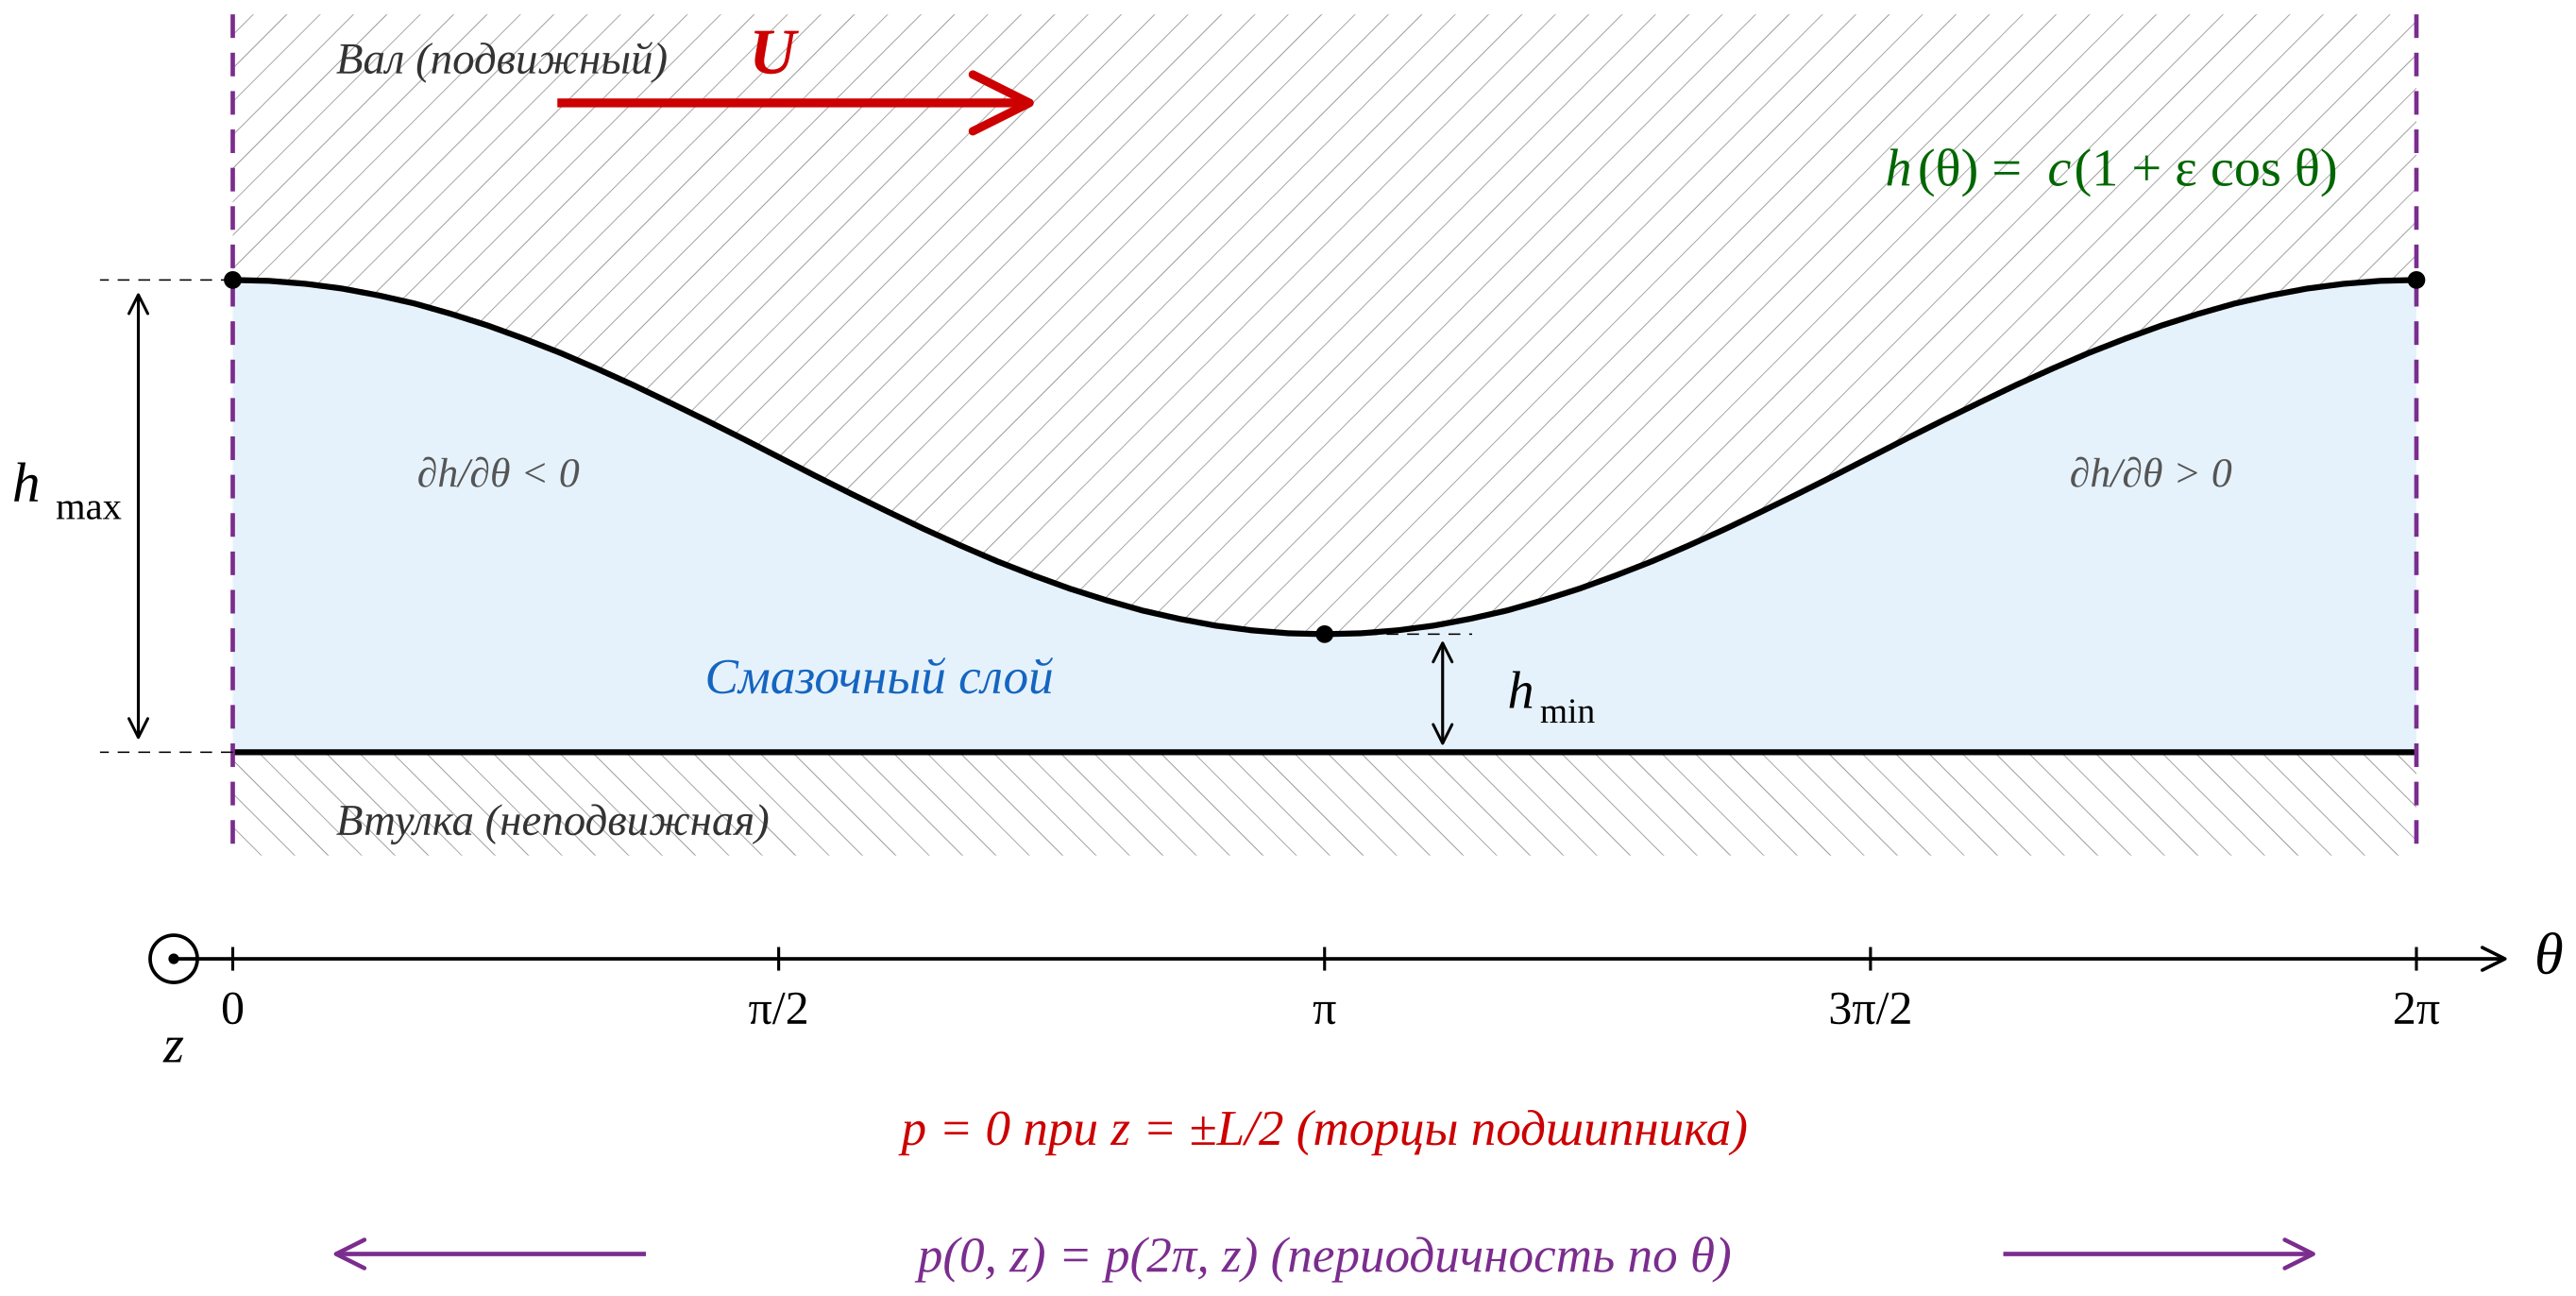
\includegraphics[width=\textwidth,height=0.9\textheight,keepaspectratio]{figures/ch02/fig_2_6.png}
\caption{Развёрнутый вид расчётной области радиального подшипника}
\label{fig:journal_unwrapped}
\end{figure}


\subsubsection*{Кинематика движения поверхностей}

Вал вращается с постоянной угловой скоростью~$\omega$ внутри неподвижной втулки. Окружная скорость поверхности вала составляет:
\begin{equation}
U = \omega\,R.
\label{eq:journal_U}
\end{equation}

Осевые скорости обеих поверхностей равны нулю. В стационарном режиме положение вала фиксировано: $\varepsilon = \mathrm{const}$, и нормальные скорости поверхностей обращаются в нуль, что исключает эффект выжимания ($\partial h/\partial t = 0$). При нестационарном анализе (динамика ротора) эксцентриситет $\varepsilon$ и угол нагрузки $\varphi$ зависят от времени, и в правой части уравнения Рейнольдса появляется squeeze-term $\partial h/\partial t$; такой случай выходит за рамки настоящего раздела.

Динамическая вязкость смазки полагается постоянной: $\mu = \mathrm{const}$ (допущение~6 из подраздела~2.1.1). Влияние температурной зависимости вязкости $\mu(T)$ рассматривается в главе~4.

Вращение вала создаёт увлекающий (куэттовский) поток смазки в окружном направлении. В зоне сходящегося зазора ($0 < \theta < \pi$, где толщина уменьшается от $h_{\max}$ к $h_{\min}$) условие неразрывности приводит к росту давления. В зоне расходящегося зазора ($\pi < \theta < 2\pi$) давление стремится к отрицательным значениям, однако физически отрицательное давление не реализуется: жидкость разрывается и образуется кавитационная зона. Именно сочетание клинового эффекта и кавитации определяет распределение давления и несущую способность радиального подшипника.


\subsubsection*{Закон толщины смазочного слоя}

Толщина смазочного слоя определяется геометрией двух эксцентричных цилиндров -- вала и втулки. При условии тонкого зазора ($c/R \ll 1$, что согласуется с допущением~3 из подраздела~2.1.1) и пренебрежении членами порядка $(c/R)^2$ и выше, толщина зазора записывается в виде:
\begin{equation}
h(\theta) = c\,(1 + \varepsilon\,\cos\theta),
\label{eq:journal_h}
\end{equation}
\begin{conditions}
$c = R_b - R$ -- радиальный зазор;\\
$\varepsilon = e/c$ -- относительный эксцентриситет.
\end{conditions}
Из формулы~\eqref{eq:journal_h} следует:
\begin{itemize}
\item максимальная толщина зазора $h_{\max} = c(1 + \varepsilon)$ достигается при $\theta = 0$ (точка, диаметрально противоположная минимальному зазору);
\item минимальная толщина зазора $h_{\min} = c(1 - \varepsilon)$ достигается при $\theta = \pi$ (точка наибольшего сближения вала и втулки).
\end{itemize}

Толщина зазора~\eqref{eq:journal_h} не зависит от осевой координаты~$z$, что соответствует осевой однородности геометрии (вал и втулка имеют цилиндрическую форму с параллельными осями). Зависимость $h$ от $z$ может возникать при перекосе вала (misalignment), однако этот случай в настоящей работе не рассматривается.

В общем случае, при наличии детерминированных микроструктур на рабочей поверхности, толщина смазочного слоя записывается как суперпозиция:
\begin{equation}
h(\theta, z) = c\,(1 + \varepsilon\,\cos\theta) + \Delta h(\theta, z),
\label{eq:journal_h_textured}
\end{equation}
где $\Delta h(\theta, z)$ -- добавка, описывающая геометрию микроструктуры (раздел~2.2).

Для характеристики геометрии радиального подшипника вводятся следующие безразмерные параметры:
\begin{itemize}
\item $\varepsilon = e/c$ -- относительный эксцентриситет, являющийся основным параметром нагружения ($\varepsilon = 0$ соответствует концентричному расположению, $\varepsilon \to 1$ -- контакту поверхностей);
\item $\psi = c/R$ -- относительный зазор (для типичных подшипников $\psi \sim 10^{-3}$);
\item $L/D$ -- отношение длины подшипника к диаметру ($D = 2R$), определяющее степень влияния осевых утечек: при $L/D > 1$ подшипник считается длинным, при $L/D < 0{,}5$ -- коротким, промежуточные значения соответствуют подшипнику конечной длины.
\end{itemize}


\subsubsection*{Уравнение Рейнольдса для радиального подшипника}

Обобщённое уравнение Рейнольдса~\eqref{eq:reynolds_full}, полученное в подразделе~2.1.1 в декартовых координатах, необходимо переписать для цилиндрической поверхности зазора радиального подшипника. Введём дуговую координату $x = R\theta$ (расстояние вдоль окружности вала), вдоль которой производная принимает вид $\partial/\partial x = (1/R)\,\partial/\partial\theta$. Осевая координата~$z$ остаётся без изменений.

В рассматриваемой задаче втулка неподвижна ($U_1 = 0$), вал движется с окружной скоростью $U_2 = \omega R = U$; осевые скорости обеих поверхностей равны нулю ($W_1 = W_2 = 0$). В стационарном режиме ($\partial h/\partial t = 0$) правая часть обобщённого уравнения Рейнольдса содержит единственный член:
\begin{equation}
\frac{U_1 + U_2}{2}\,\frac{1}{R}\,\frac{\partial h}{\partial \theta} = \frac{U}{2R}\,\frac{\partial h}{\partial \theta} = \frac{\omega}{2}\,\frac{\partial h}{\partial \theta}.
\label{eq:journal_rhs_derivation}
\end{equation}

Стационарное уравнение Рейнольдса для несжимаемой ньютоновской жидкости в координатах $(\theta, z)$ принимает вид:
\begin{equation}
\frac{1}{R^2}\frac{\partial}{\partial \theta}\!\left[\frac{h^3}{12\mu}\,\frac{\partial p}{\partial \theta}\right] + \frac{\partial}{\partial z}\!\left[\frac{h^3}{12\mu}\,\frac{\partial p}{\partial z}\right] = \frac{\omega}{2}\,\frac{\partial h}{\partial \theta}.
\label{eq:journal_reynolds}
\end{equation}

Множитель $1/R^2$ перед первым слагаемым в левой части обусловлен двукратным применением оператора $\partial/\partial x = (1/R)\,\partial/\partial\theta$ при переходе от декартовой координаты~$x$ к угловой~$\theta$.

Умножая обе части уравнения~\eqref{eq:journal_reynolds} на~$12\mu$ (что допустимо при $\mu = \mathrm{const}$), получаем эквивалентную форму, удобную для численной реализации:
\begin{equation}
\frac{1}{R^2}\frac{\partial}{\partial \theta}\!\left[h^3\,\frac{\partial p}{\partial \theta}\right] + \frac{\partial}{\partial z}\!\left[h^3\,\frac{\partial p}{\partial z}\right] = 6\mu\omega\,\frac{\partial h}{\partial \theta}.
\label{eq:journal_reynolds_num}
\end{equation}

Уравнение~\eqref{eq:journal_reynolds_num} является основным расчётным уравнением для радиального подшипника в настоящей работе.

Подставляя конкретное выражение для толщины зазора~\eqref{eq:journal_h}, получаем производную в правой части:
\begin{equation}
\frac{\partial h}{\partial \theta} = -c\,\varepsilon\,\sin\theta.
\label{eq:journal_dh_dtheta}
\end{equation}

Правая часть уравнения~\eqref{eq:journal_reynolds_num} принимает вид $-6\mu\omega\,c\,\varepsilon\,\sin\theta$. Источниковый член в правой части пропорционален $-\sin\theta$, поэтому максимум генерации давления приходится на $\theta \approx \pi/2$, где скорость сужения зазора наибольшая. В зоне $0 < \theta < \pi$ выполняется $\partial h/\partial\theta < 0$ (сходящийся клин): зазор уменьшается по направлению вращения, и давление генерируется. В зоне $\pi < \theta < 2\pi$ выполняется $\partial h/\partial\theta > 0$ (расходящийся клин): зазор увеличивается, давление стремится к отрицательным значениям, и вступает в действие кавитация.

Левая часть уравнений~\eqref{eq:journal_reynolds}-\eqref{eq:journal_reynolds_num} представляет собой эллиптический оператор $\nabla \cdot (h^3 \nabla p)$, записанный в координатах $(\theta, z)$ на цилиндрической поверхности. По структуре он аналогичен оператору в уравнении для упорного подшипника~\eqref{eq:thrust_reynolds_num}, однако здесь вместо координат $(r, \theta)$ используются $(\theta, z)$. Правая часть -- источниковый член, пропорциональный $\sin\theta$: максимум генерации давления приходится на $\theta = \pi/2$. При $\varepsilon = 0$ (концентричное расположение вала и втулки) $\partial h/\partial \theta = 0$, правая часть обращается в нуль и давление не генерируется -- подшипник не несёт нагрузки.

Уравнение~\eqref{eq:journal_reynolds_num} допускает два классических предельных случая, для которых известны аналитические решения.

\textit{Бесконечно длинный подшипник ($L/D \to \infty$).} В этом пределе давление не зависит от осевой координаты: $\partial p/\partial z = 0$, и уравнение~\eqref{eq:journal_reynolds_num} вырождается в обыкновенное дифференциальное уравнение по~$\theta$. Полное аналитическое решение этого ОДУ с периодическими граничными условиями и без учёта кавитации известно как решение Зоммерфельда (Sommerfeld, 1904). Учёт кавитации приводит к половинному решению (half-Sommerfeld), в котором давление обнуляется в зоне расходящегося зазора.

\textit{Бесконечно короткий подшипник ($L/D \to 0$).} В этом пределе осевой градиент давления значительно превышает окружной: $\partial^2 p/\partial z^2 \gg (1/R^2)\,\partial^2 p/\partial \theta^2$, и окружной член в левой части уравнения~\eqref{eq:journal_reynolds_num} может быть опущен. Уравнение вырождается в ОДУ по~$z$ при каждом фиксированном~$\theta$, что допускает аналитическое решение. Это приближение известно как приближение Дюбуа--Оквирка (Dubois--Ocvirk, short-bearing approximation) и даёт удовлетворительные результаты при $L/D < 0{,}5$.

Для подшипника конечной длины ($0{,}5 \lesssim L/D \lesssim 2$) ни один из предельных случаев не обеспечивает достаточной точности, и уравнение~\eqref{eq:journal_reynolds_num} решается численно (глава~3).


\subsubsection*{Граничные условия}

Для замыкания уравнения Рейнольдса~\eqref{eq:journal_reynolds_num} необходимо задать граничные условия на давление по всему контуру расчётной области~\eqref{eq:journal_domain}.

\textit{По окружной координате~$\theta$.} Область по~$\theta$ охватывает полную окружность, поэтому естественным условием является периодичность:
\begin{equation}
p(0, z) = p(2\pi, z), \quad \frac{\partial p}{\partial \theta}\bigg|_{\theta=0} = \frac{\partial p}{\partial \theta}\bigg|_{\theta=2\pi}.
\label{eq:journal_bc_periodic}
\end{equation}

\textit{По осевой координате~$z$.} На торцах подшипника давление принимается равным атмосферному:
\begin{equation}
p(\theta,\,-L/2) = 0, \quad p(\theta,\,L/2) = 0,
\label{eq:journal_bc_axial}
\end{equation}
где давление отсчитывается от атмосферного ($p = p_{\mathrm{abs}} - p_{\mathrm{atm}}$), как и в подразделе~2.1.2. При наличии принудительной подачи смазки через осевую канавку условие на соответствующем угле $\theta = \theta_{\mathrm{groove}}$ модифицируется: $p(\theta_{\mathrm{groove}}, z) = p_{\mathrm{sup}}$, где $p_{\mathrm{sup}}$ -- давление подачи. Помимо условий Дирихле на торцах, в специальных конструкциях могут применяться условия непротекания $q_z = 0$, эквивалентные $\partial p/\partial z = 0$ (при наличии уплотнений на торцах подшипника), или смешанные условия, когда на части окружности задаётся давление подачи, а на остальной -- атмосферное давление.

\textit{Кавитация.} Принципиальной особенностью радиального подшипника является неизбежное возникновение кавитации в зоне расходящегося зазора ($\pi < \theta < 2\pi$), где расчётное давление стремится к отрицательным значениям. В простейшей постановке применяют ограничение $p \geq 0$ (условие Гюмбеля), при котором отрицательные давления обнуляются после решения. Более физичным является условие Рейнольдса (Swift--Stieber), требующее одновременного выполнения $p = 0$ и $\partial p/\partial \theta = 0$ на границе кавитации. Оба подхода, однако, не обеспечивают точного сохранения массы. Корректная массо-сохраняющая постановка, основанная на модели Jakobsson--Floberg--Olsson (JFO), вводится в разделе~2.3.

Граница кавитационной зоны является внутренней границей задачи, положение которой заранее неизвестно и определяется в процессе решения. Периодичность задаётся как граничное условие на контуре области~\eqref{eq:journal_domain}, а кавитационная зона является внутренней частью решения. Само поле давления $p(\theta, z)$ при этом остаётся непрерывным и периодическим, хотя и состоит из двух участков: зоны полного смазочного слоя ($p > 0$) и зоны кавитации ($p = 0$). Качественное распределение давления $p(\theta)$ в среднем сечении подшипника ($z = 0$) показано на рисунке~\ref{fig:journal_pressure_profile}.

% [РИСУНОК: Качественный профиль давления в радиальном подшипнике]
% Должен показывать:
% - Ось абсцисс: θ от 0 до 2π
% - p(θ) при z=0: рост в зоне 0 < θ < π, максимум вблизи θ = π/2
% - Зона кавитации: p = 0 при π < θ < 2π (приблизительно)
% - Границы разрыва и восстановления
% - Пунктир: полное решение Зоммерфельда (без кавитации, отрицательные давления)
\begin{figure}[!ht]
\centering
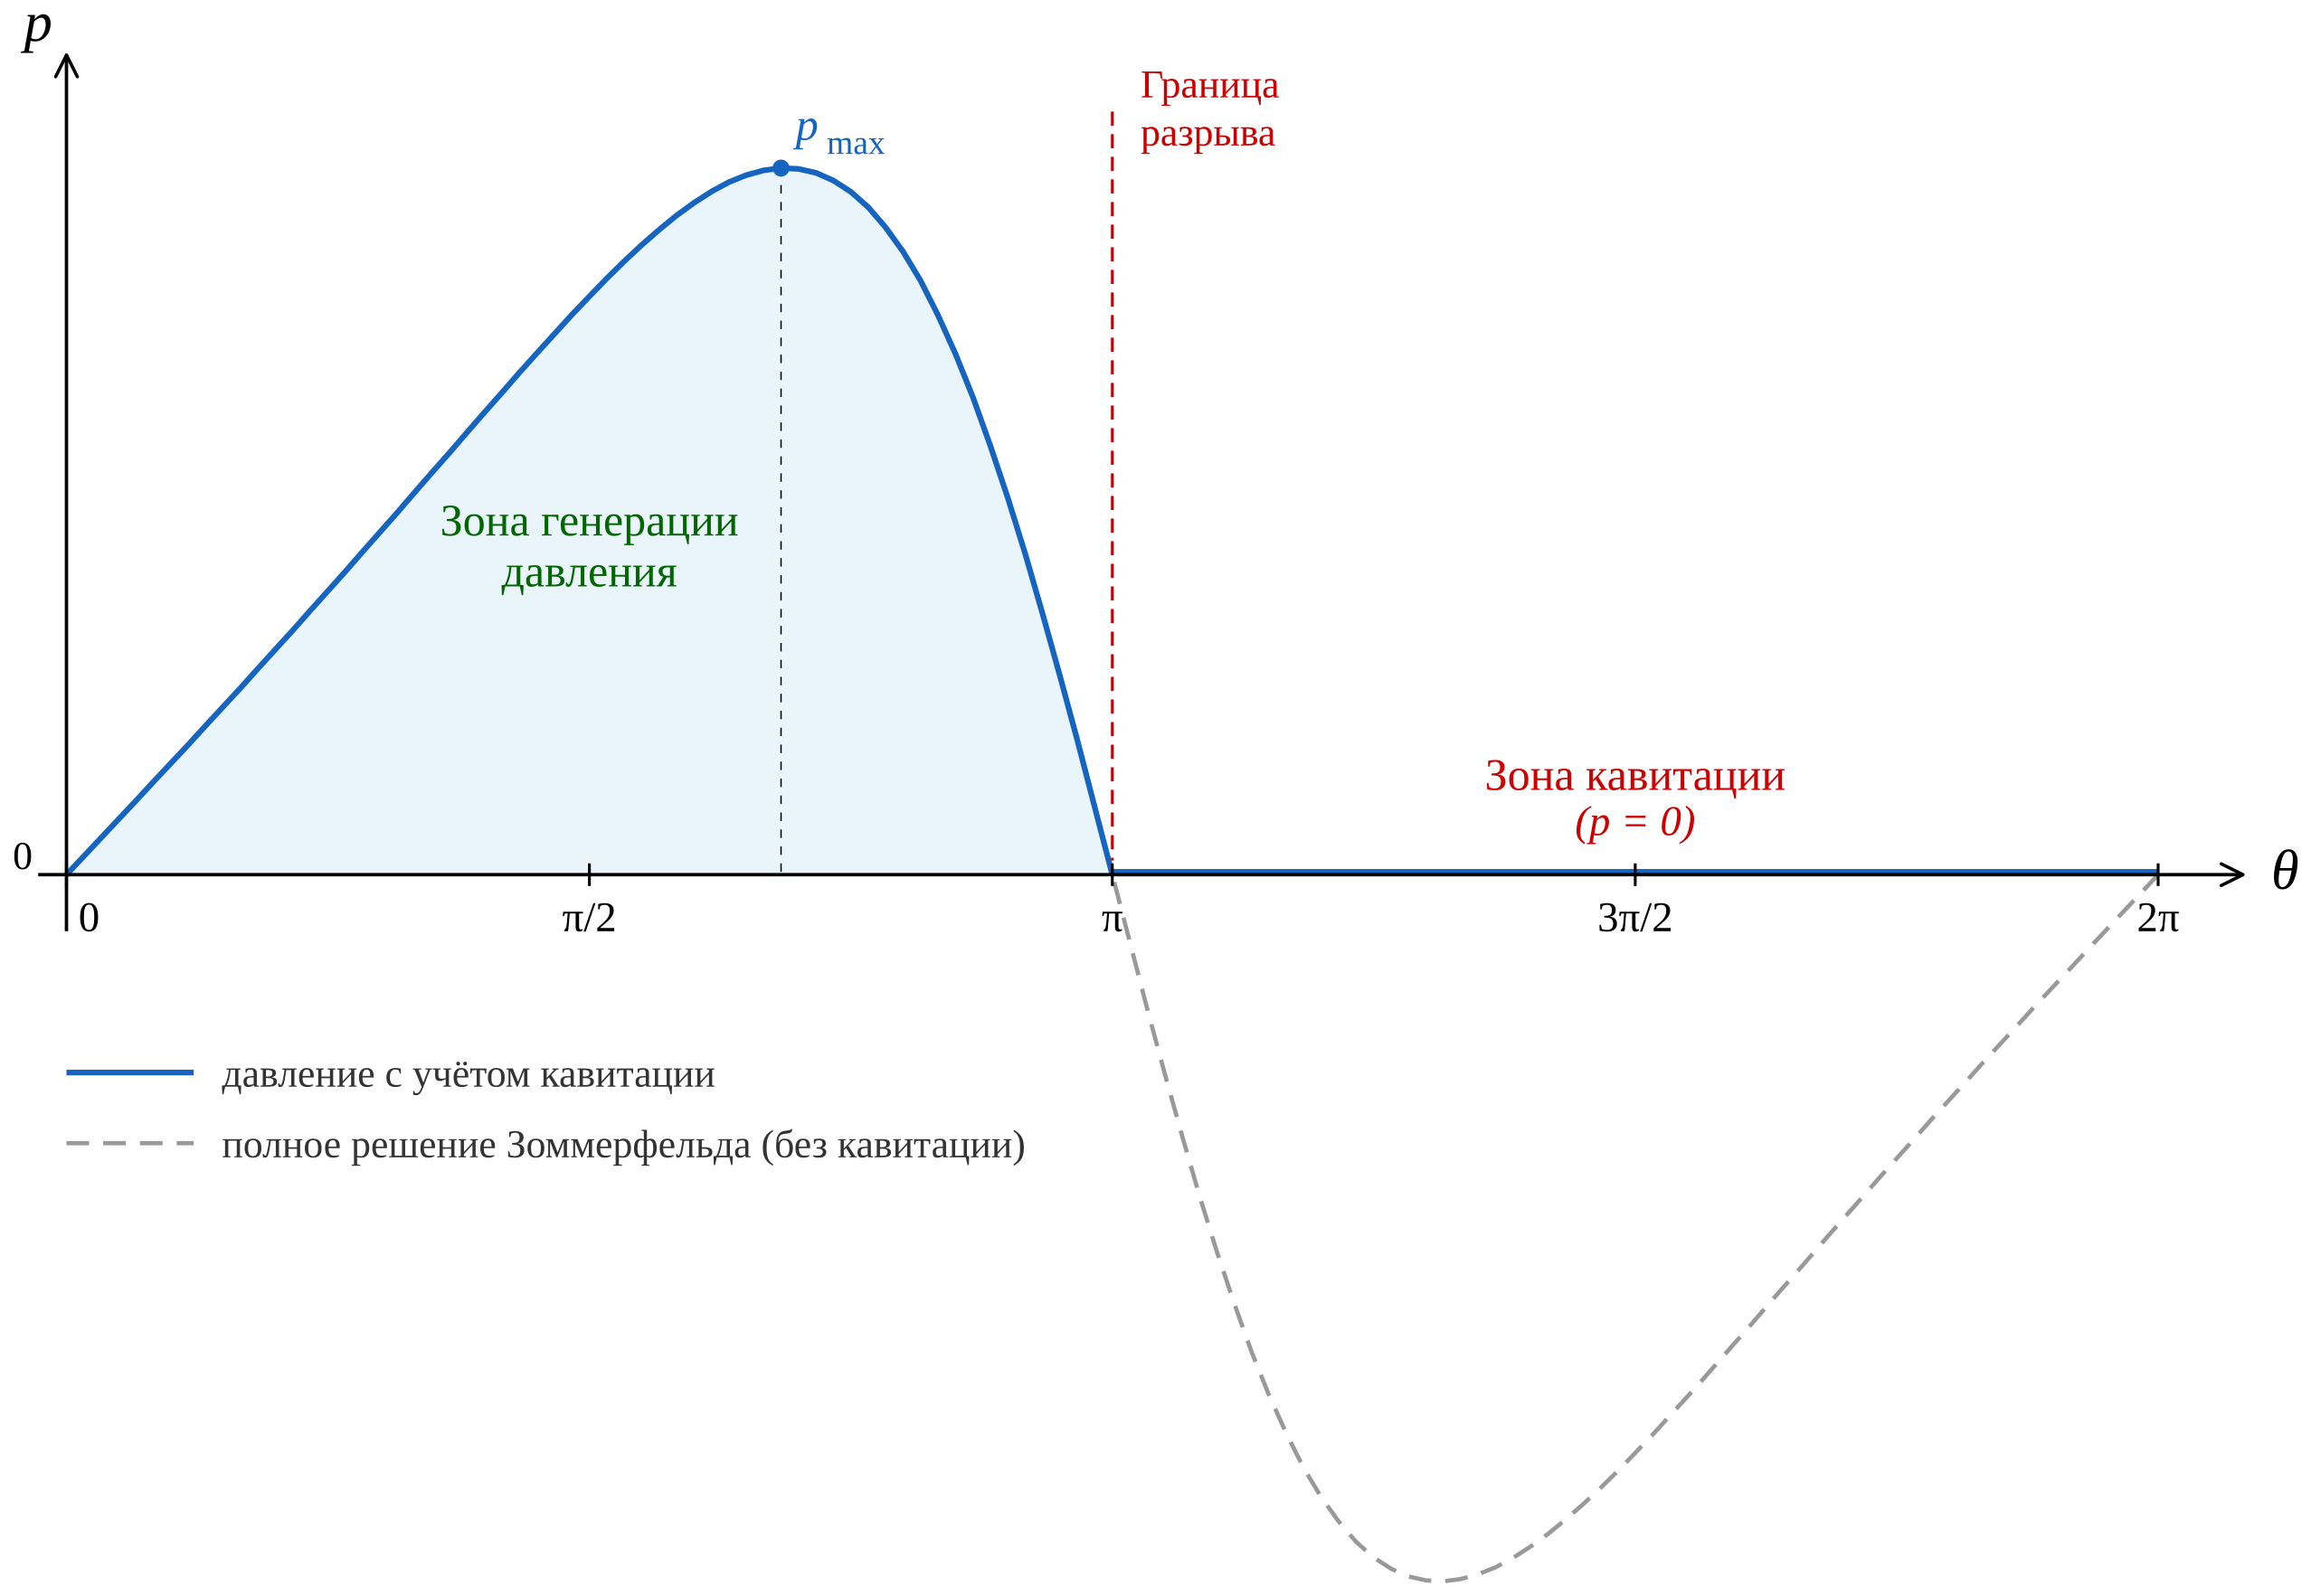
\includegraphics[width=\textwidth,height=0.9\textheight,keepaspectratio]{figures/ch02/fig_2_7.png}
\caption{Качественное распределение давления в радиальном подшипнике и зона кавитации}
\label{fig:journal_pressure_profile}
\end{figure}


\subsubsection*{Объёмные расходы}

Объёмные расходы жидкости через единицу длины определяются путём интегрирования профилей скорости по толщине смазочного слоя, аналогично подразделу~2.1.2.

Окружной расход (на единицу длины по осевой координате~$z$):
\begin{equation}
\label{eq:journal_q_theta}
q_\theta(\theta, z) = \frac{h\,U}{2} - \frac{h^3}{12\mu\,R}\,\frac{\partial p}{\partial \theta} = \frac{h\,\omega R}{2} - \frac{h^3}{12\mu\,R}\,\frac{\partial p}{\partial \theta}.
\end{equation}

Первое слагаемое представляет куэттовскую составляющую расхода, обусловленную увлечением жидкости вращающимся валом; второе -- пуазейлевскую составляющую, определяемую окружным градиентом давления. Множитель $1/R$ во втором слагаемом обусловлен переходом от производной по дуге $\partial/\partial(R\theta)$ к производной по углу $\partial/\partial\theta$.

Осевой расход (на единицу длины по окружной координате):
\begin{equation}
q_z(\theta, z) = -\frac{h^3}{12\mu}\,\frac{\partial p}{\partial z}.
\label{eq:journal_q_z}
\end{equation}

Поскольку осевые скорости обеих поверхностей равны нулю, осевой расход полностью определяется градиентом давления (пуазейлевская составляющая). Именно осевой расход обусловливает боковую утечку смазки через торцы подшипника.

Суммарная утечка через торцы подшипника определяется интегрированием осевого расхода по окружности:
\begin{equation}
Q_{\mathrm{side}} = \int_0^{2\pi} \bigl[ q_z(\theta,\,L/2) - q_z(\theta,\,-L/2) \bigr]\,R\,\mathrm{d}\theta.
\label{eq:journal_Q_side}
\end{equation}

Множитель $R\,\mathrm{d}\theta$ соответствует элементу длины дуги на окружности вала. Здесь $q_z(\theta, L/2) > 0$ соответствует потоку, вытекающему через торец $z = L/2$ (по направлению внешней нормали $+\mathbf{e}_z$), а $q_z(\theta, -L/2) < 0$ -- потоку, вытекающему через торец $z = -L/2$ (нормаль $-\mathbf{e}_z$). Обозначая утечки через отдельные торцы как $Q_+ = \int_0^{2\pi} q_z(\theta, L/2)\,R\,\mathrm{d}\theta$ и $Q_- = -\int_0^{2\pi} q_z(\theta, -L/2)\,R\,\mathrm{d}\theta$, получаем $Q_{\mathrm{side}} = Q_+ + Q_-$.

При симметрии давления относительно средней плоскости подшипника ($p(\theta, z) = p(\theta, -z)$) утечки через оба торца одинаковы, и выражение~\eqref{eq:journal_Q_side} упрощается:
\begin{equation}
Q_{\mathrm{side}} = 2\int_0^{2\pi} q_z(\theta,\,L/2)\,R\,\mathrm{d}\theta.
\label{eq:journal_Q_side_sym}
\end{equation}

Боковая утечка является основным механизмом потери смазки в радиальном подшипнике. При уменьшении отношения $L/D$ доля давления, <<разгружаемая>> через торцы, возрастает, что снижает несущую способность. В предельном случае бесконечно короткого подшипника ($L/D \to 0$) осевые утечки полностью доминируют, и именно это обстоятельство позволяет пренебречь окружным членом в уравнении Рейнольдса (приближение Дюбуа--Оквирка).

Баланс массы в стационарном режиме без выжимания записывается в дифференциальной форме (аналогично уравнению~\eqref{eq:thrust_mass_balance} для упорного подшипника):
\begin{equation}
\frac{1}{R}\,\frac{\partial q_\theta}{\partial \theta} + \frac{\partial q_z}{\partial z} = 0.
\label{eq:journal_mass_balance}
\end{equation}

Подстановка выражений~\eqref{eq:journal_q_theta} и~\eqref{eq:journal_q_z} в уравнение~\eqref{eq:journal_mass_balance} приводит к уравнению Рейнольдса~\eqref{eq:journal_reynolds}.


Решение уравнения Рейнольдса даёт поле давления~$p$ в расчётной области. По найденному давлению вычисляются интегральные характеристики узла: несущая способность, расходы смазки, силы и моменты трения, минимальная толщина плёнки. Унифицированные формулы для всех выходных величин приведены в подразделе~2.1.7.

В практической постановке задачи внешняя радиальная нагрузка $\mathbf{W}_{\mathrm{ext}}$ и параметры режима ($\omega$, $\mu$, $c$, $R$, $L$) считаются заданными, тогда как положение вала $(\varepsilon, \varphi)$ является неизвестным. Равновесное положение определяется из условия статического баланса сил: $\mathbf{W}(\varepsilon, \varphi) = -\mathbf{W}_{\mathrm{ext}}$, т.\,е. из системы двух нелинейных уравнений относительно $\varepsilon$ и $\varphi$. Численное решение этой системы методом итерационного поиска описывается в главе~3.

Сформулированная задача сводится к решению эллиптического уравнения Рейнольдса~\eqref{eq:journal_reynolds_num} в прямоугольной области~\eqref{eq:journal_domain} с периодическими условиями по окружной координате~$\theta$ и условиями Дирихле по осевой координате~$z$. Принципиальной особенностью радиального подшипника, отличающей его от упорного (подраздел~2.1.2), является неизбежное возникновение кавитации в зоне расходящегося зазора: при любом ненулевом эксцентриситете $\varepsilon > 0$ правая часть уравнения Рейнольдса меняет знак, и в отсутствие ограничений на давление решение содержит области с $p < 0$~\cite{gao2014}.

Численная дискретизация уравнения~\eqref{eq:journal_reynolds_num} методом конечных разностей и алгоритм учёта кавитации на основе модели JFO рассматриваются в главе~3. При наличии микроструктур на рабочей поверхности функция зазора~\eqref{eq:journal_h_textured} приобретает быстрые локальные вариации, параметризация которых описывается в разделе~2.2.

\FloatBarrier
\subsection{Постановка задачи для радиального зазора при возвратно-поступательном движении}

Рассмотрим узел трения с осевым возвратно-поступательным относительным движением поверхностей: плунжер (поршень, шток) совершает возвратно-поступательное перемещение внутри цилиндра (втулки). Тонкий слой вязкой жидкости заполняет кольцевой зазор между сопряжёнными цилиндрическими поверхностями и выполняет функцию смазки и уплотнения.

Узлы данного типа широко распространены в машиностроении. В плунжерных насосах высокого давления зазор между плунжером и гильзой одновременно уплотняет рабочую жидкость и обеспечивает смазку. В гидроцилиндрах поршень перемещается внутри гильзы под действием давления рабочей жидкости. В поршневых компрессорах и двигателях внутреннего сгорания поршень с кольцами образует трибологическую пару скольжения с гильзой цилиндра. В направляющих скольжения металлорежущих станков возвратно-поступательное движение суппорта или стола сопровождается формированием смазочного слоя~\cite{hori2002,szeri1998}.

Ключевое отличие рассматриваемой постановки от подразделов~2.1.2-2.1.3 состоит в следующем. Скорость увлечения $U(t)$ меняет знак при реверсе хода, вследствие чего клиновой член в правой части уравнения Рейнольдса меняет знак: зона повышенного давления <<переезжает>> от одного конца рабочей зоны к другому. При каждом реверсе возможны разрыв и последующее восстановление сплошности смазочного слоя. Второе существенное отличие -- нестационарный squeeze-член $\partial h/\partial t$ зачастую играет определяющую роль: колебания эксцентриситета, вибрации и перекос плунжера приводят к изменению зазора во времени, что генерирует давление даже при отсутствии клинового эффекта. Все общие допущения, принятые при выводе уравнения Рейнольдса, наследуются из подраздела~2.1.1.


\subsubsection*{Геометрия и система координат}

Основными геометрическими параметрами узла являются:
\begin{itemize}
\item $R$ -- радиус плунжера;
\item $R_b$ -- радиус внутренней поверхности цилиндра (втулки);
\item $c = R_b - R$ -- радиальный зазор;
\item $L$ -- длина рабочей зоны контакта (длина втулки);
\item $e(t)$ -- эксцентриситет (расстояние между осями плунжера и цилиндра), в общем случае зависящий от времени;
\item $\varepsilon(t) = e(t)/c$ -- относительный эксцентриситет;
\item $\varphi(t)$ -- угол положения линии центров.
\end{itemize}

Для описания задачи используется цилиндрическая система координат $(\theta, z, y)$:
\begin{itemize}
\item $z$ -- ось движения плунжера (вдоль хода), $z \in [0,\; L]$;
\item $\theta$ -- окружная координата, $\theta \in [0,\; 2\pi]$;
\item $y$ -- координата по толщине смазочного слоя, направленная от поверхности цилиндра ($y = 0$) к поверхности плунжера ($y = h$).
\end{itemize}

Область расчёта представляет собой прямоугольник:
\begin{equation}
\theta \in [0,\; 2\pi], \quad z \in [0,\; L].
\label{eq:recip_domain}
\end{equation}

В отличие от радиального подшипника (подраздел~2.1.3), где основное течение является окружным ($\theta$-направление), вызванным вращением вала, а утечка -- осевой ($z$), в возвратно-поступательном узле картина обратная: основное течение направлено вдоль оси $z$ и вызвано поступательным движением плунжера, а окружное течение является вторичным, обусловленным неоднородностью давления по~$\theta$. Схема узла представлена на рис.~\ref{fig:recip_scheme}.

% [РИСУНОК: Схема возвратно-поступательного узла]
\begin{figure}[!ht]
\centering
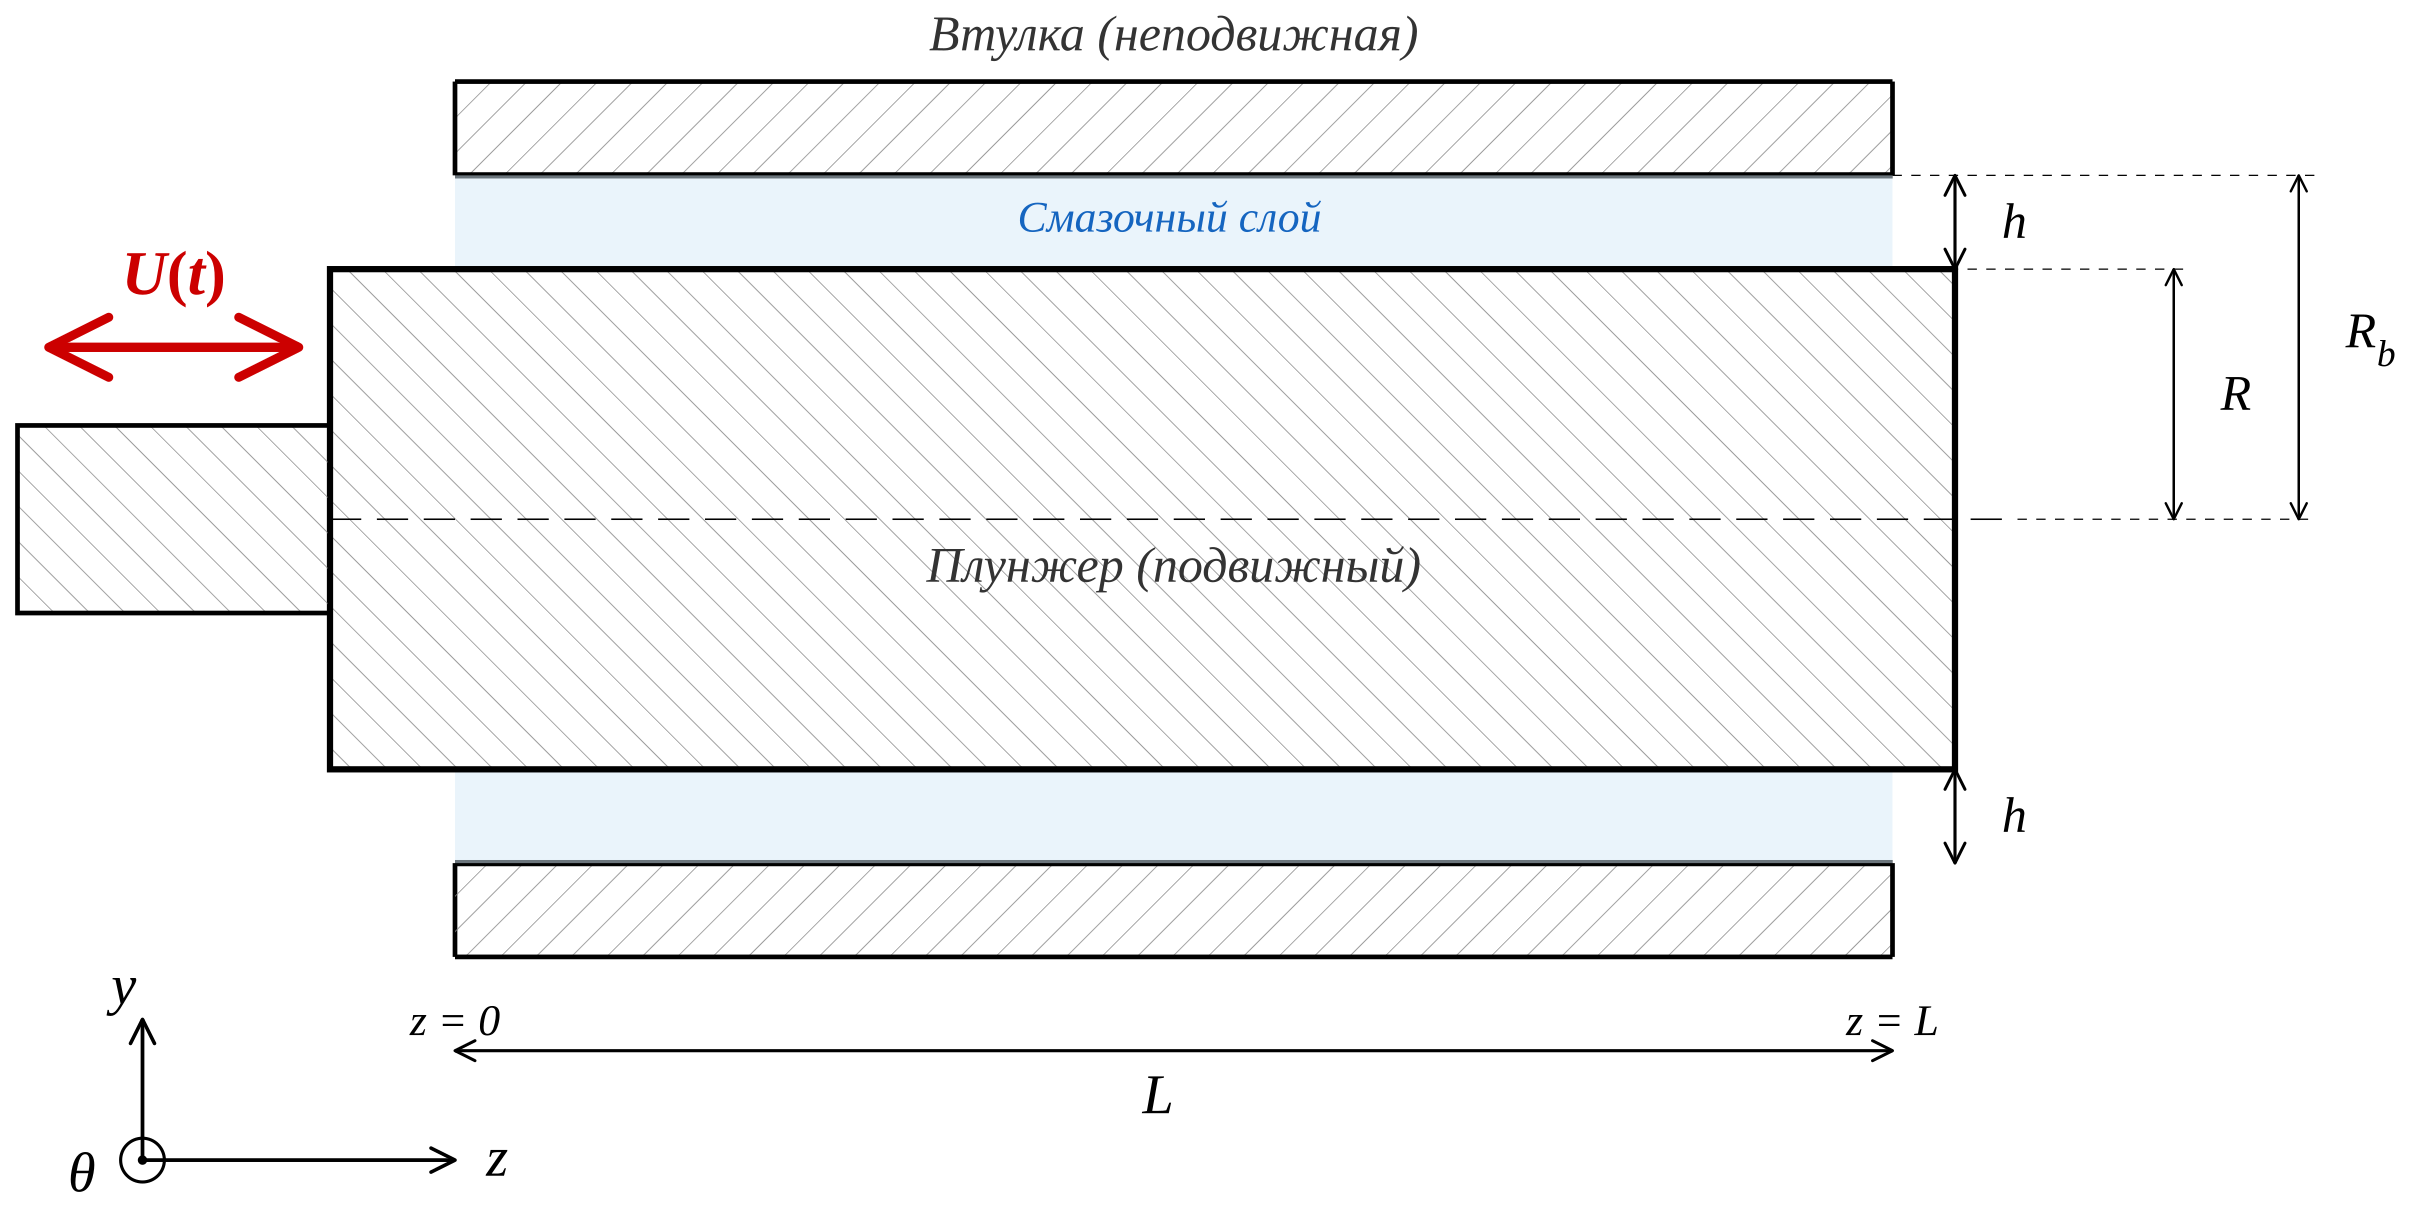
\includegraphics[width=\textwidth,height=0.9\textheight,keepaspectratio]{figures/ch02/fig_2_8.png}
\caption{Схема возвратно-поступательного узла: плунжер внутри цилиндрической втулки}
\label{fig:recip_scheme}
\end{figure}


\subsubsection*{Кинематика движения}

Закон хода плунжера задаётся функцией положения $s(t)$; скорость поступательного движения определяется как
\begin{equation}
U(t) = \frac{ds}{dt}.
\label{eq:recip_U}
\end{equation}

Типичный гармонический закон хода, удобный для верификации численных схем:
\begin{equation}
s(t) = \frac{S}{2}\bigl(1 - \cos(\Omega t)\bigr), \quad
U(t) = \frac{S\,\Omega}{2}\sin(\Omega t),
\label{eq:recip_harmonic}
\end{equation}
\begin{conditions}
$S$ -- полный ход (stroke);\\
$\Omega$ -- угловая частота возвратно-поступательного движения.
\end{conditions}
В реальных механизмах закон $s(t)$ может определяться кинематикой кривошипно-шатунного механизма, однако для модели достаточно задать $U(t)$ произвольной функцией времени.


\subsubsection*{Закон толщины смазочного слоя}

Базовая геометрия описывается двумя эксцентричными цилиндрами -- плунжером и втулкой, аналогично радиальному подшипнику (подраздел~2.1.3):
\begin{equation}
h(\theta, t) = c\bigl(1 + \varepsilon(t)\cos(\theta - \varphi(t))\bigr).
\label{eq:recip_h_base}
\end{equation}

Для возникновения клинового эффекта вдоль оси~$z$ необходима неоднородность $\partial h/\partial z \neq 0$. Источниками такой неоднородности являются: конусность (taper) зазора, перекос оси плунжера, микропрофиль поверхности, а также специально введённый рельеф (микротекстура, см.\ раздел~2.2).

Общий вид толщины зазора с учётом осевой конусности:
\begin{equation}
h(\theta, z, t) = c\bigl(1 + \varepsilon(t)\cos(\theta - \varphi(t))\bigr) + \kappa\Bigl(z - \frac{L}{2}\Bigr),
\label{eq:recip_h_tilt}
\end{equation}
где $\kappa$ -- параметр осевой конусности зазора (taper). При $\kappa > 0$ зазор увеличивается от середины к торцу $z = L$; при $\kappa < 0$ -- уменьшается. При $\kappa = 0$ клин вдоль $z$ отсутствует; давление может генерироваться только через squeeze-член ($\partial h/\partial t \neq 0$).
Параметры $\varepsilon$ и $\kappa$ должны удовлетворять условию $h(\theta, z, t) > 0$ по всей расчётной области; в частности, необходимо $\varepsilon < 1$ и $|\kappa|\,L/2 < c\,(1 - \varepsilon)$.

При наличии детерминированных микроструктур на рабочей поверхности толщина зазора записывается как суперпозиция:
\begin{equation}
h(\theta, z, t) = h_{\mathrm{base}}(\theta, z, t) + \Delta h(\theta, z),
\label{eq:recip_h_textured}
\end{equation}
где $\Delta h(\theta, z)$ -- добавка, описывающая геометрию микроструктуры (подробно в разделе~2.2).

Производная по времени от базового зазора~\eqref{eq:recip_h_tilt} при постоянной конусности ($\kappa = \mathrm{const}$) определяется изменением эксцентриситета и угла линии центров:
\begin{equation}
\frac{\partial h}{\partial t}
= c\bigl[\dot{\varepsilon}(t)\cos(\theta - \varphi(t))
       + \varepsilon(t)\,\dot{\varphi}(t)\sin(\theta - \varphi(t))\bigr],
\label{eq:recip_dhdt}
\end{equation}
\begin{conditions}
$\dot{\varepsilon} = d\varepsilon/dt$;\\
$\dot{\varphi} = d\varphi/dt$.
\end{conditions}
Слагаемое с конусностью $\kappa$ не вносит вклада в $\partial h/\partial t$, поскольку $\kappa$ не зависит от времени. При фиксированном положении плунжера ($\dot{\varepsilon} = 0$, $\dot{\varphi} = 0$) squeeze-член обращается в нуль, и давление генерируется только клиновым эффектом.


\subsubsection*{Уравнение Рейнольдса}

На цилиндрической поверхности зазора в координатах $(\theta, z)$ при осевом увлечении со скоростью $U(t)$ и отсутствии окружного увлечения уравнение Рейнольдса для несжимаемой ньютоновской жидкости принимает вид:
\begin{equation}
\frac{1}{R^2}\frac{\partial}{\partial\theta}
  \biggl(\frac{h^3}{12\mu}\frac{\partial p}{\partial\theta}\biggr)
+ \frac{\partial}{\partial z}
  \biggl(\frac{h^3}{12\mu}\frac{\partial p}{\partial z}\biggr)
= \frac{U(t)}{2}\frac{\partial h}{\partial z}
+ \frac{\partial h}{\partial t}.
\label{eq:recip_reynolds}
\end{equation}
Здесь $R$ -- радиус плунжера; ввиду малости зазора ($c \ll R$) замена $R$ на $R_b$ не вносит существенной погрешности.

Умножая обе части на~$12\mu$, получаем эквивалентную форму, удобную для численной реализации:
\begin{equation}
\frac{1}{R^2}\frac{\partial}{\partial\theta}
  \biggl(h^3\frac{\partial p}{\partial\theta}\biggr)
+ \frac{\partial}{\partial z}
  \biggl(h^3\frac{\partial p}{\partial z}\biggr)
= 6\mu\,U(t)\frac{\partial h}{\partial z}
+ 12\mu\frac{\partial h}{\partial t}.
\label{eq:recip_reynolds_num}
\end{equation}

Правая часть уравнения~\eqref{eq:recip_reynolds_num} содержит два слагаемых различной физической природы.

Первый член $6\mu\,U(t)\,\partial h/\partial z$ описывает клиновой эффект: давление генерируется при наличии сужения зазора вдоль направления движения ($\partial h/\partial z \neq 0$). При реверсе хода ($U < 0$) знак этого члена меняется на противоположный, и область повышенного давления <<переезжает>> от одного конца рабочей зоны к другому (рис.~\ref{fig:recip_reversal}). Именно этот механизм определяет несущую способность клинового зазора.

% [РИСУНОК: Реверс зоны давления при смене знака U(t)]
\begin{figure}[!ht]
\centering
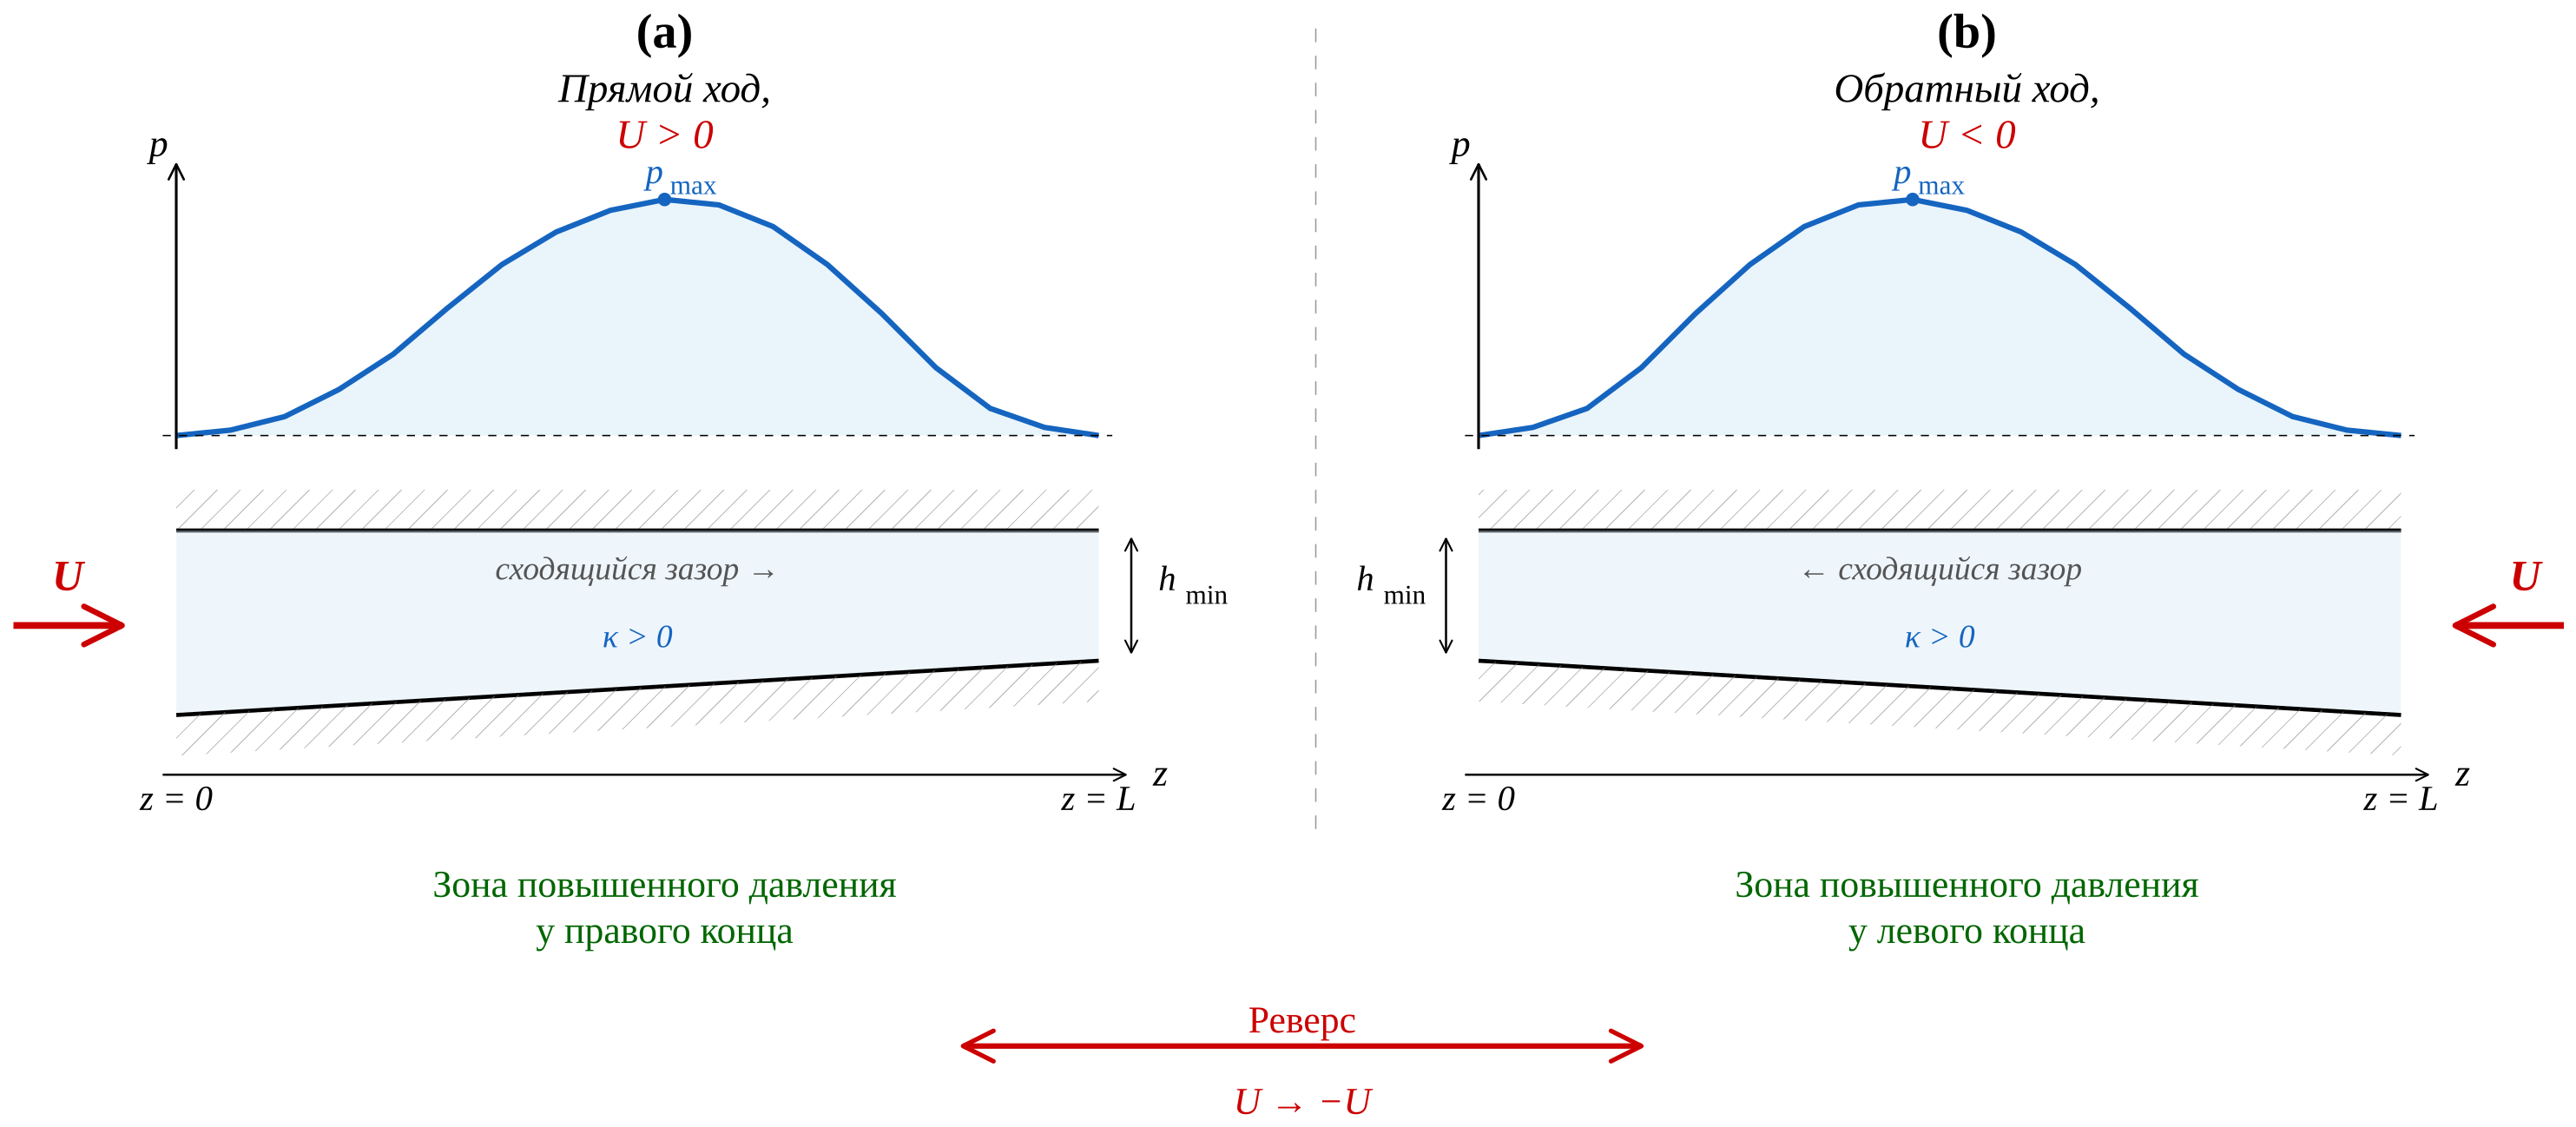
\includegraphics[width=\textwidth,height=0.9\textheight,keepaspectratio]{figures/ch02/fig_2_9.png}
\caption{Смена направления скорости $U(t)$ приводит к перемещению зоны повышенного давления: (a)~прямой ход ($U>0$); (b)~обратный ход ($U<0$). Клин вдоль~$z$ обусловлен конусностью~$\kappa$}
\label{fig:recip_reversal}
\end{figure}

\FloatBarrier

Второй член $12\mu\,\partial h/\partial t$ описывает squeeze-эффект (эффект выжимания): давление генерируется при сближении поверхностей ($\partial h/\partial t < 0$), даже если клиновой зазор вдоль $z$ отсутствует. Этот механизм важен при колебаниях эксцентриситета, вибрациях и перекосе плунжера. При удалении поверхностей ($\partial h/\partial t > 0$) данный член стремится понизить давление, что способствует возникновению кавитации.

По структуре уравнение~\eqref{eq:recip_reynolds_num} аналогично уравнениям для упорного~\eqref{eq:thrust_reynolds_num} и радиального~\eqref{eq:journal_reynolds_num} подшипников: левая часть содержит эллиптический оператор $\nabla \cdot (h^3 \nabla p)$, а правая -- источниковые члены. Отличие состоит в направлении увлечения (осевое вместо окружного) и в явной нестационарности правой части.


\subsubsection*{Граничные условия}

\textit{По окружной координате~$\theta$.} Область по~$\theta$ охватывает полную окружность, поэтому естественным условием является периодичность:
\begin{equation}
p(0, z, t) = p(2\pi, z, t), \quad
\frac{\partial p}{\partial\theta}\bigg|_{\theta=0}
= \frac{\partial p}{\partial\theta}\bigg|_{\theta=2\pi}.
\label{eq:recip_bc_periodic}
\end{equation}

\textit{По осевой координате~$z$.} Рассматриваются три варианта.

\textit{(a) Открытые торцы (атмосферные кромки, базовый вариант):}
\begin{equation}
p(\theta, 0, t) = 0, \quad p(\theta, L, t) = 0.
\label{eq:recip_bc_open}
\end{equation}

Давление отсчитывается от атмосферного ($p = p_{\mathrm{abs}} - p_{\mathrm{atm}}$), как и в подразделах~2.1.2-2.1.3. Данный вариант соответствует свободным кромкам втулки, открытым в окружающую среду.

\textit{(b) Давление подачи/слива (гидросистема):}
\begin{equation}
p(\theta, 0, t) = p_{\mathrm{in}}(t), \quad p(\theta, L, t) = p_{\mathrm{out}}(t).
\label{eq:recip_bc_pressure}
\end{equation}

Такая постановка типична для гидроцилиндров, где полости с обеих сторон поршня находятся под рабочим давлением.

\textit{(c) Уплотнённые торцы (отсутствие протекания):}
\begin{equation}
\frac{\partial p}{\partial z}\bigg|_{z=0} = 0, \quad
\frac{\partial p}{\partial z}\bigg|_{z=L} = 0.
\label{eq:recip_bc_sealed}
\end{equation}

Условие непротекания $q_z = 0$ на торцах эквивалентно $\partial p/\partial z = 0$ и применяется при наличии уплотнительных элементов на кромках втулки.

\textit{Кавитация.} При реверсе скорости и в расходящихся участках зазора давление стремится стать отрицательным. Простое ограничение $p \geq 0$ (условие Гюмбеля) нарушает баланс массы на границе кавитационной зоны. Корректный массо-сохраняющий учёт кавитации обеспечивается моделью JFO, вводимой в разделе~2.3.


\subsubsection*{Объёмные расходы}

Удельные потоки (расходы на единицу длины) определяются путём интегрирования профилей скорости по толщине смазочного слоя, аналогично подразделам~2.1.2-2.1.3.

Осевой расход (на единицу длины по окружной координате):
\begin{equation}
q_z(\theta, z, t) = \frac{h\,U(t)}{2}
  - \frac{h^3}{12\mu}\frac{\partial p}{\partial z}.
\label{eq:recip_q_z}
\end{equation}

Первое слагаемое представляет куэттовскую составляющую, обусловленную движением плунжера; второе -- пуазейлевскую составляющую, определяемую осевым градиентом давления.

Окружной расход (на единицу длины по осевой координате):
\begin{equation}
q_\theta(\theta, z, t) = -\frac{h^3}{12\mu R}\frac{\partial p}{\partial\theta}.
\label{eq:recip_q_theta}
\end{equation}

Поскольку окружные скорости обеих поверхностей равны нулю (плунжер совершает только поступательное движение), куэттовская составляющая в окружном направлении отсутствует. Окружной расход полностью определяется градиентом давления.

Полная утечка через торцы рабочей зоны:
\begin{equation}
\label{eq:recip_Q_leakage}
\begin{split}
&Q_{\mathrm{out}}(t) = \int_0^{2\pi} q_z(\theta,\,L,\,t)\,R\,\mathrm{d}\theta, \\
&Q_{\mathrm{in}}(t) = \int_0^{2\pi} q_z(\theta,\,0,\,t)\,R\,\mathrm{d}\theta.
\end{split}
\end{equation}

Знаки определяются направлением внешней нормали, как и в подразделах~2.1.2-2.1.3: положительный $Q_{\mathrm{out}}$ соответствует вытеканию смазки из рабочей зоны через торец $z = L$.

Решение уравнения Рейнольдса даёт поле давления $p(\theta, z, t)$. По найденному давлению вычисляются интегральные характеристики узла: несущая способность, расходы смазки, силы и моменты трения, минимальная толщина плёнки. Унифицированные формулы для всех выходных величин приведены в подразделе~2.1.7.

Для возвратно-поступательных узлов микротекстурирование поверхностей рассматривается как способ повышения несущей способности и снижения утечек; параметризация микрорельефа вводится в разделе~2.2.

\FloatBarrier
\subsection{Область применимости модели}

Допущения, положенные в основу уравнения Рейнольдса, перечислены в подразделе~2.1.1 (п.~1-8). Ниже для каждого из них указаны условия, при которых допущение может нарушаться, и соответствующие расширения модели. Часть расширений реализована в последующих разделах и главах настоящей работы.

\subsubsection*{Геометрия тонкого слоя}

Смазочная аппроксимация предполагает малость отношения $\epsilon = H/L \ll 1$, где $H$ -- характерная толщина смазочного слоя (подраздел~2.1.1), и малые уклоны поверхностей $|\partial h/\partial x| \ll 1$, $|\partial h/\partial z| \ll 1$. При широких зазорах, очень коротких контактах или наличии резких кромок и ступенек эти условия нарушаются, и необходимо обращаться к CFD-моделированию на основе полных уравнений Навье--Стокса. Локальные большие уклоны, связанные с микроструктурами (раздел~2.2), формально выходят за рамки классической смазочной аппроксимации. На практике применение уравнения Рейнольдса остаётся корректным, если глубина микроструктуры $h_p$ мала по сравнению с зазором ($h_p / h_0 \ll 1$), а длина переходного участка $\ell_p$ обеспечивает малость уклона: $|\partial h/\partial x| \sim h_p/\ell_p \ll 1$.

\subsubsection*{Инерция}

Инерционные члены пренебрежимо малы при $\mathrm{Re}\,\epsilon \ll 1$, см.~\eqref{eq:Re_epsilon}. При высоких скоростях, низкой вязкости или увеличенном зазоре этот параметр растёт, и инерционные эффекты становятся существенными. В таких случаях применяются инерционные поправки к уравнению Рейнольдса или переход к полным уравнениям Навье--Стокса. В типичных режимах подшипников скольжения, рассматриваемых в настоящей работе, малость зазора ($\epsilon \ll 1$) и умеренные скорости обеспечивают $\mathrm{Re}\,\epsilon \ll 1$.

\subsubsection*{Ламинарность}

С ростом скорости и зазора или при снижении вязкости течение может утратить устойчивость и перейти в турбулентный режим. В турбулентном режиме обычно модифицируют расходные соотношения, вводя эффективные коэффициенты потока, что приводит к <<турбулентному>> уравнению Рейнольдса (подходы Hirs, Ng--Pan). В настоящей работе рассматривается ламинарный режим, характерный для подшипников скольжения при малых зазорах.

\subsubsection*{Несжимаемость}

При газовой смазке или при высоких давлениях, вызывающих заметное изменение плотности, допущение $\rho = \mathrm{const}$ нарушается. Сжимаемая форма уравнения Рейнольдса записывается через баланс массы:
\begin{equation}
\frac{\partial (\rho h)}{\partial t}
+ \frac{\partial (\rho\, q_x)}{\partial x}
+ \frac{\partial (\rho\, q_z)}{\partial z} = 0,
\label{eq:reynolds_compressible}
\end{equation}
где $q_x$ и $q_z$ -- удельные расходы~\eqref{eq:flow_rate_x},~\eqref{eq:flow_rate_z}. При $\rho = \mathrm{const}$ уравнение~\eqref{eq:reynolds_compressible} сводится к уже полученному уравнению~\eqref{eq:reynolds_full}. Для жидких смазочных материалов при умеренных давлениях плотность практически постоянна. В настоящей работе рассматривается несжимаемая жидкость.

\subsubsection*{Постоянная вязкость и изотермичность}

Интенсивный сдвиг в тонкой смазочной плёнке может приводить к значительному вязкостному нагреву. В этом случае вязкость становится функцией температуры, $\mu = \mu(T)$, и уравнение Рейнольдса необходимо решать совместно с уравнением энергии -- термогидродинамическая (THD) постановка. При высоких контактных давлениях существенной становится пьезовязкость $\mu = \mu(p)$, характерная для упругогидродинамической смазки (EHL). В обобщённом уравнении Рейнольдса~\eqref{eq:reynolds_full} вязкость записана под знаком производных, что обеспечивает корректность формулы и при переменной вязкости $\mu = \mu(x, z)$. Влияние температурной зависимости вязкости рассматривается в главе~4.

\subsubsection*{Условие прилипания}

При очень малых зазорах (порядка десятков нанометров) или при наличии специальных покрытий (гидрофобных, олеофобных) возможно проскальзывание жидкости на стенке (Navier slip). В данной работе скольжение на границе не учитывается.

\subsubsection*{Жёсткие поверхности}

Модель предполагает геометрически заданный зазор $h(x, z, t)$, не зависящий от давления. При высоких нагрузках или использовании податливых материалов упругая деформация поверхностей изменяет форму зазора, что приводит к упругогидродинамической (EHL) постановке: уравнение Рейнольдса решается совместно с уравнением упругости. В настоящей работе поверхности полагаются жёсткими.

\subsubsection*{Кавитация}

В областях расходящегося зазора давление, полученное из уравнения Рейнольдса, может становиться отрицательным, что физически соответствует разрыву сплошности смазочного слоя (кавитации). Простое ограничение $p \geq 0$ (условие Гюмбеля) нарушает баланс массы на границе кавитационной зоны. Массо-сохраняющий подход Jakobsson--Floberg--Olsson (JFO), обеспечивающий корректное описание кавитации, вводится в разделе~2.3.

В рамках настоящей работы базовые допущения расширяются в следующих направлениях:
\begin{itemize}
  \item кавитация и массо-сохранение -- раздел~2.3;
  \item микроструктуры поверхности -- раздел~2.2;
  \item температурная зависимость вязкости $\mu(T)$ -- глава~4.
\end{itemize}
Упругие деформации поверхностей (EHL), турбулентность, сжимаемость и скольжение на границе в рамках настоящей работы не рассматриваются.

Допущения модели Рейнольдса, условия их нарушения и возможные
расширения систематизированы
в таблице~\ref{tab:model_limits}.

\begin{table}[!ht]
\centering
\caption{Допущения модели Рейнольдса, условия их применимости
  и возможные расширения}
\label{tab:model_limits}
\begin{tabularx}{\textwidth}{|X|X|X|}
\hline
\multicolumn{1}{|c|}{\textbf{Допущение}}
  & \multicolumn{1}{c|}{\textbf{Когда нарушается}}
  & \multicolumn{1}{c|}{\textbf{Расширение модели}} \\
\hline
Изотермическая смазка ($T = T_0$, $\mu = \mathrm{const}$)
  & Высокие нагрузки и скорости, интенсивная вязкостная
    диссипация
  & THD-постановка (уравнение энергии) \\
\hline
Ньютоновская смазка
  & Добавки к смазке, высокие скорости сдвига
    ($\dot\gamma > 10^5$~с$^{-1}$)
  & Модели Карро, Эйри и~др. \\
\hline
Несжимаемость ($\rho = \mathrm{const}$)
  & Давление порядка $0{,}5$~ГПа и выше (EHL-режим)
  & Уравнение Тейта для $\rho(p)$ \\
\hline
Постоянная вязкость
  & Пьезовязкостные смазки, давление выше $0{,}1$~ГПа
  & Уравнение Баруса $\mu = \mu_0 e^{\alpha p}$ \\
\hline
Гладкие поверхности
  & Смешанный/граничный режим ($\lambda_r = h/\sigma < 3$)
  & Осреднённое уравнение Патира--Ченга \\
\hline
Ламинарное течение
  & Число Рейнольдса плёнки $Re_f > 1$
    ($Re_f = \rho U h / \mu$)
  & Турбулентные поправки \\
\hline
\end{tabularx}
\end{table}

\FloatBarrier

Принятые допущения соответствуют классической
гидродинамической теории смазки Рейнольдса и обоснованы для
жидкостного и смешанного режимов при умеренных давлениях
($p < 50$~МПа) и скоростях ($Re_f < 1$). По сравнению
с прямым CFD-моделированием тонкого смазочного слоя (решение
уравнений Навье--Стокса в трёхмерной постановке) уравнение
Рейнольдса на несколько порядков дешевле при сопоставимой
точности в зоне своей применимости. Это принципиально важно
для параметрических расчётов, оптимизации геометрии
микроструктур и анализа динамических коэффициентов, где
требуется многократное решение задачи~\cite{hori2002,suddapalli2015}.

\FloatBarrier
\subsection{Безразмерная постановка}

Переход к безразмерным переменным унифицирует три частные постановки, сформулированные в подразделах~2.1.2-2.1.4, и позволяет сравнивать различные конфигурации подшипников и режимы их работы на единой шкале. Кроме того, безразмеризация сокращает число определяющих параметров задачи до нескольких безразмерных групп, что упрощает параметрический анализ. Введённый аппарат используется далее при исследовании влияния микроструктур поверхности (раздел~2.2) и при численной дискретизации (глава~3).

\subsubsection*{Характерные масштабы и безразмерные переменные}

Общая схема масштабирования повторяет подход, применённый при выводе уравнения Рейнольдса в подразделе~2.1.1~\cite{hori2002,szeri1998}, но теперь записывается в обобщённых обозначениях, пригодных для всех трёх постановок:
%
\begin{equation}
\bar{s}_1 = \frac{s_1}{L_1}, \quad
\bar{s}_2 = \frac{s_2}{L_2}, \quad
\bar{h}   = \frac{h}{h_0},   \quad
\bar{p}   = \frac{p}{p_0},   \quad
\bar{U}   = \frac{U}{U_0},   \quad
\bar{t}   = \frac{t}{t_0},
\label{eq:nondim_vars}
\end{equation}
%
\begin{conditions}
$s_1$, $s_2$ -- поверхностные координаты (конкретные для каждой постановки, см.\ таблицу~\ref{tab:nondim_scales} ниже);\\
$h_0$ -- характерная толщина зазора (радиальный зазор $c$ или средний зазор);\\
$U_0$ -- характерная скорость увлечения;\\
$t_0$ -- характерное время (для нестационарных задач).
\end{conditions}
Масштаб давления выбирается так, чтобы клиновой член в правой части уравнения Рейнольдса имел порядок единицы. Из баланса~\eqref{eq:pressure_scale} следует:
%
\begin{equation}
p_0 = \frac{6\,\mu_0\,U_0\,L_1}{h_0^2},
\label{eq:nondim_p0}
\end{equation}
%
\begin{conditions}
$L_1$ -- масштаб длины вдоль направления увлечения (координата $s_1$);\\
$\mu_0$ -- характерное значение вязкости.
\end{conditions}

\subsubsection*{Безразмерное уравнение Рейнольдса}

Подставляя масштабы~\eqref{eq:nondim_vars},~\eqref{eq:nondim_p0} в обобщённое уравнение Рейнольдса~\eqref{eq:reynolds_full} и сокращая размерные множители, получаем единую безразмерную форму:
%
\begin{equation}
\frac{\partial}{\partial \bar{s}_1}\!\left(\bar{h}^{\,3}\,\frac{\partial \bar{p}}{\partial \bar{s}_1}\right)
+ \Lambda^2\,\frac{\partial}{\partial \bar{s}_2}\!\left(\bar{h}^{\,3}\,\frac{\partial \bar{p}}{\partial \bar{s}_2}\right)
= \bar{U}\,\frac{\partial \bar{h}}{\partial \bar{s}_1}
+ \sigma\,\frac{\partial \bar{h}}{\partial \bar{t}},
\label{eq:reynolds_nondim}
\end{equation}
%
где введены две безразмерные группы:
%
\begin{equation}
\Lambda = \frac{L_1}{L_2}
\label{eq:nondim_Lambda}
\end{equation}
%
-- параметр удлинённости (aspect ratio), характеризующий соотношение продольного и поперечного масштабов, и
%
\begin{equation}
\sigma = \frac{2\,L_1}{U_0\,t_0}
\label{eq:nondim_sigma}
\end{equation}
%
-- параметр нестационарности (squeeze number), определяющий относительный вклад выжимания плёнки.

При $\sigma = 0$ (либо в стационарной задаче) член выжимания отсутствует, и уравнение содержит только клиновой источник. Параметр $\Lambda$ определяет относительный вклад поперечного растекания: при $\Lambda \ll 1$ вклад второго члена мал и задача приближается к одномерной по $s_1$; при $\Lambda \gg 1$ доминирует поперечное растекание по $s_2$, что соответствует <<короткому>> приближению в терминологии радиального подшипника (подраздел~2.1.3). Для цилиндрических координат, используемых в постановках~2.1.2-2.1.4, в левой части уравнения~\eqref{eq:reynolds_nondim} появляются дополнительные множители $1/\bar{r}$ и $1/\bar{r}^{\,2}$, однако общая структура уравнения сохраняется.

\subsubsection*{Масштабы для частных постановок}

Конкретные значения масштабов для трёх постановок, рассмотренных в подразделах~2.1.2-2.1.4, приведены в таблице~\ref{tab:nondim_scales}.

\begin{table}[!ht]
\centering
\caption{Характерные масштабы для безразмерной постановки}
\label{tab:nondim_scales}
\resizebox{\textwidth}{!}{%
\begin{tabular}{|l|c|c|c|c|c|c|c|c|}
\hline
\multicolumn{1}{|c|}{\textbf{Постановка}} & $\boldsymbol{s_1}$ & $\boldsymbol{s_2}$ & $\boldsymbol{L_1}$ & $\boldsymbol{L_2}$ & $\boldsymbol{h_0}$ & $\boldsymbol{U_0}$ & $\boldsymbol{p_0}$ & $\boldsymbol{t_0}$ \\
\hline
Упорная (2.1.2)
  & $R\theta$ & $r$ & $R$ & $R_{\mathrm{out}} - R_{\mathrm{in}}$
  & $h_{\min}$ или $h_{\mathrm{mean}}$
  & $\omega R$ & $\dfrac{6\mu_0\omega R^2}{h_0^2}$ & --
\\[6pt]
\hline
Радиальная (2.1.3)
  & $R\theta$ & $z$ & $R$ & $L$
  & $c$
  & $\omega R$ & $\dfrac{6\mu_0\omega R^2}{c^2}$ & --
\\[6pt]
\hline
Возвратно-пост.\ (2.1.4)
  & $z$ & $R\theta$ & $L$ & $R$
  & $c$
  & $\max|U(t)|$ & $\dfrac{6\mu_0\,U_0\,L}{c^2}$ & $1/\Omega$
\\[6pt]
\hline
\end{tabular}%
}
\end{table}

\FloatBarrier

В упорной и радиальной постановках задача стационарна, поэтому временной масштаб $t_0$ не требуется (обозначено <<-->>{} в таблице). Координата $s_1$ соответствует направлению увлечения, а $s_2$ -- поперечному направлению. Для упорного подшипника $R$ -- характерный радиус (например, $R_{\mathrm{out}}$ или среднее значение $(R_{\mathrm{in}} + R_{\mathrm{out}})/2$). При подстановке масштабов из таблицы в общее уравнение~\eqref{eq:reynolds_nondim} получаются безразмерные формы, согласованные с размерными уравнениями~\eqref{eq:thrust_reynolds_num},~\eqref{eq:journal_reynolds_num},~\eqref{eq:recip_reynolds_num}.

Характерный масштаб давления~$p_0 = 6\mu_0 U_0 L_1 / h_0^2$
(формула~\eqref{eq:nondim_p0}) определяет, при каких реальных
давлениях безразмерное поле~$P$ имеет порядок единицы.
Для радиального подшипника насоса (глава~5): $\mu_0 = 0{,}01105$~Па$\cdot$с,
$U_0 = \omega R = 10{,}9$~м/с, $L_1 = R = 0{,}035$~м,
$h_0 = c = 50$~мкм:
%
\begin{equation}
  p_0 = \frac{6 \cdot 0{,}01105 \cdot 10{,}9
    \cdot 0{,}035}{(50 \cdot 10^{-6})^2}
  \approx 10{,}1 \;\text{МПа}.
  \label{eq:p0_example}
\end{equation}
%
Максимальные безразмерные давления в расчётах глав 5--6 имеют
порядок $10^{-1}$, что соответствует размерным значениям
порядка единиц мегапаскалей,~-- в пределах применимости
изотермической постановки. Для упорного подшипника (глава~7)
масштаб~$p_0$ иной вследствие меньшего характерного зазора
и другой скорости, что объясняет различие в абсолютных
значениях несущей способности при схожих безразмерных уровнях
давления.

Параметр $\Lambda = L_1/L_2$~\eqref{eq:nondim_Lambda}
физически характеризует соотношение «продольного»
и «поперечного» масштабов задачи вдоль направления увлечения
и поперёк него (таблица~\ref{tab:nondim_scales}).
Для радиального подшипника $L_1 = R$, $L_2 = L$ (длина
подшипника), поэтому $\Lambda = R/L$. При малых $\Lambda$
($R \ll L$, узкий и длинный подшипник) поперечным растеканием
можно пренебречь, и задача сводится к одномерной по~$s_1$~--
это «бесконечно длинное» приближение. При больших $\Lambda$
($R \gg L$, широкий и короткий подшипник) давление быстро
выравнивается по~$s_1$, и поперечный градиент определяет
структуру течения~-- это «короткое» приближение. Для реальных
подшипников $L/D \approx 0{,}5$--$1{,}5$, откуда
$\Lambda \approx 0{,}33$--$1{,}0$, что соответствует
промежуточному режиму с существенным вкладом обоих членов
в уравнении~\eqref{eq:reynolds_nondim}.

Введённые масштабы определяют безразмерную форму уравнения Рейнольдса и базовой геометрии зазора. Параметры, характеризующие микроструктуры поверхности, -- безразмерная глубина $h_p/h_0$, размеры элементов, плотность покрытия -- вводятся отдельно в подразделе~2.2.4. Далее в работе, если не оговорено иное, используются безразмерные переменные; черта над символом опускается для краткости записи.

\FloatBarrier
\subsection{Целевые функционалы и выходные величины}

Решение уравнения Рейнольдса даёт поле давления $p(s_1, s_2, t)$
в смазочном слое. По найденному давлению и известной геометрии
зазора $h(s_1, s_2, t)$ вычисляются интегральные характеристики узла,
определяющие его работоспособность и энергоэффективность.
В настоящем подразделе приведены унифицированные формулы
для всех трёх постановок (2.1.2-2.1.4).

Элемент площади $dA$ для каждой постановки:
\begin{itemize}
  \item упорная (2.1.2): $dA = r\,dr\,d\theta$,\quad
        $r \in [R_{\mathrm{in}},\,R_{\mathrm{out}}]$,\;
        $\theta \in [0,\,2\pi]$;
  \item радиальная (2.1.3): $dA = R\,d\theta\,dz$,\quad
        $\theta \in [0,\,2\pi]$,\; $z \in [0,\,L]$;
  \item возвратно-поступательная (2.1.4): $dA\!=\!R\,d\theta\,dz$,\,
        $\theta\!\in\![0,\,2\pi]$,\, $z\!\in\![0,\,L]$.
\end{itemize}

%% ===== Блок 1: Несущая способность =====
\subsubsection*{Несущая способность}

Для упорного подшипника результирующая нагрузка направлена вдоль оси
вращения и является скалярной величиной:
\begin{equation}
  W = \iint_A p\,dA
    = \int_0^{2\pi}\!\int_{R_{\mathrm{in}}}^{R_{\mathrm{out}}}
      p(r,\theta)\,r\,dr\,d\theta.
  \label{eq:func_W_thrust}
\end{equation}

Для радиального и возвратно-поступательного подшипников давление
распределено по цилиндрической поверхности, поэтому результирующая
сила имеет две компоненты в плоскости поперечного сечения.
Нормаль к поверхности вала направлена радиально наружу:
$\mathbf{n} = (\cos\theta,\,\sin\theta)$.
Гидродинамическая сила, действующая на вал со стороны смазочного слоя,
определяется как:
Поскольку давление действует на поверхность вала по направлению
внутрь ($d\mathbf{F} = -p\,\mathbf{n}\,dA$), компоненты силы
содержат знак <<минус>>:
\begin{equation}
\begin{alignedat}{2}
  & F_x(t) &\;=\;& -\int_0^L \int_0^{2\pi}
    p(\theta,z,t)\,\cos\theta\;R\,d\theta\,dz, \\
  & F_y(t) &\;=\;& -\int_0^L \int_0^{2\pi}
    p(\theta,z,t)\,\sin\theta\;R\,d\theta\,dz, \\
  & F(t)   &\;=\;& \sqrt{F_x^2(t) + F_y^2(t)}.
\end{alignedat}
  \label{eq:func_F_components}
\end{equation}
Здесь ось $x$ соответствует направлению $\theta = 0$,
ось $y$ -- направлению $\theta = \pi/2$.
Угол нагружения (attitude angle):
\begin{equation}
  \psi(t) = \mathrm{atan2}\bigl(F_y(t),\,F_x(t)\bigr).
  \label{eq:func_psi}
\end{equation}

Угол $\psi$ определяет направление результирующей гидродинамической
силы относительно оси $x$ и используется при анализе орбит вала
(главы~5-8).
Для стационарного радиального подшипника зависимость от $t$ отсутствует.
Схема компонент силы показана на рис.~\ref{fig:force_components}.

% [РИСУНОК: Компоненты гидродинамической силы]
\begin{figure}[!ht]
\centering
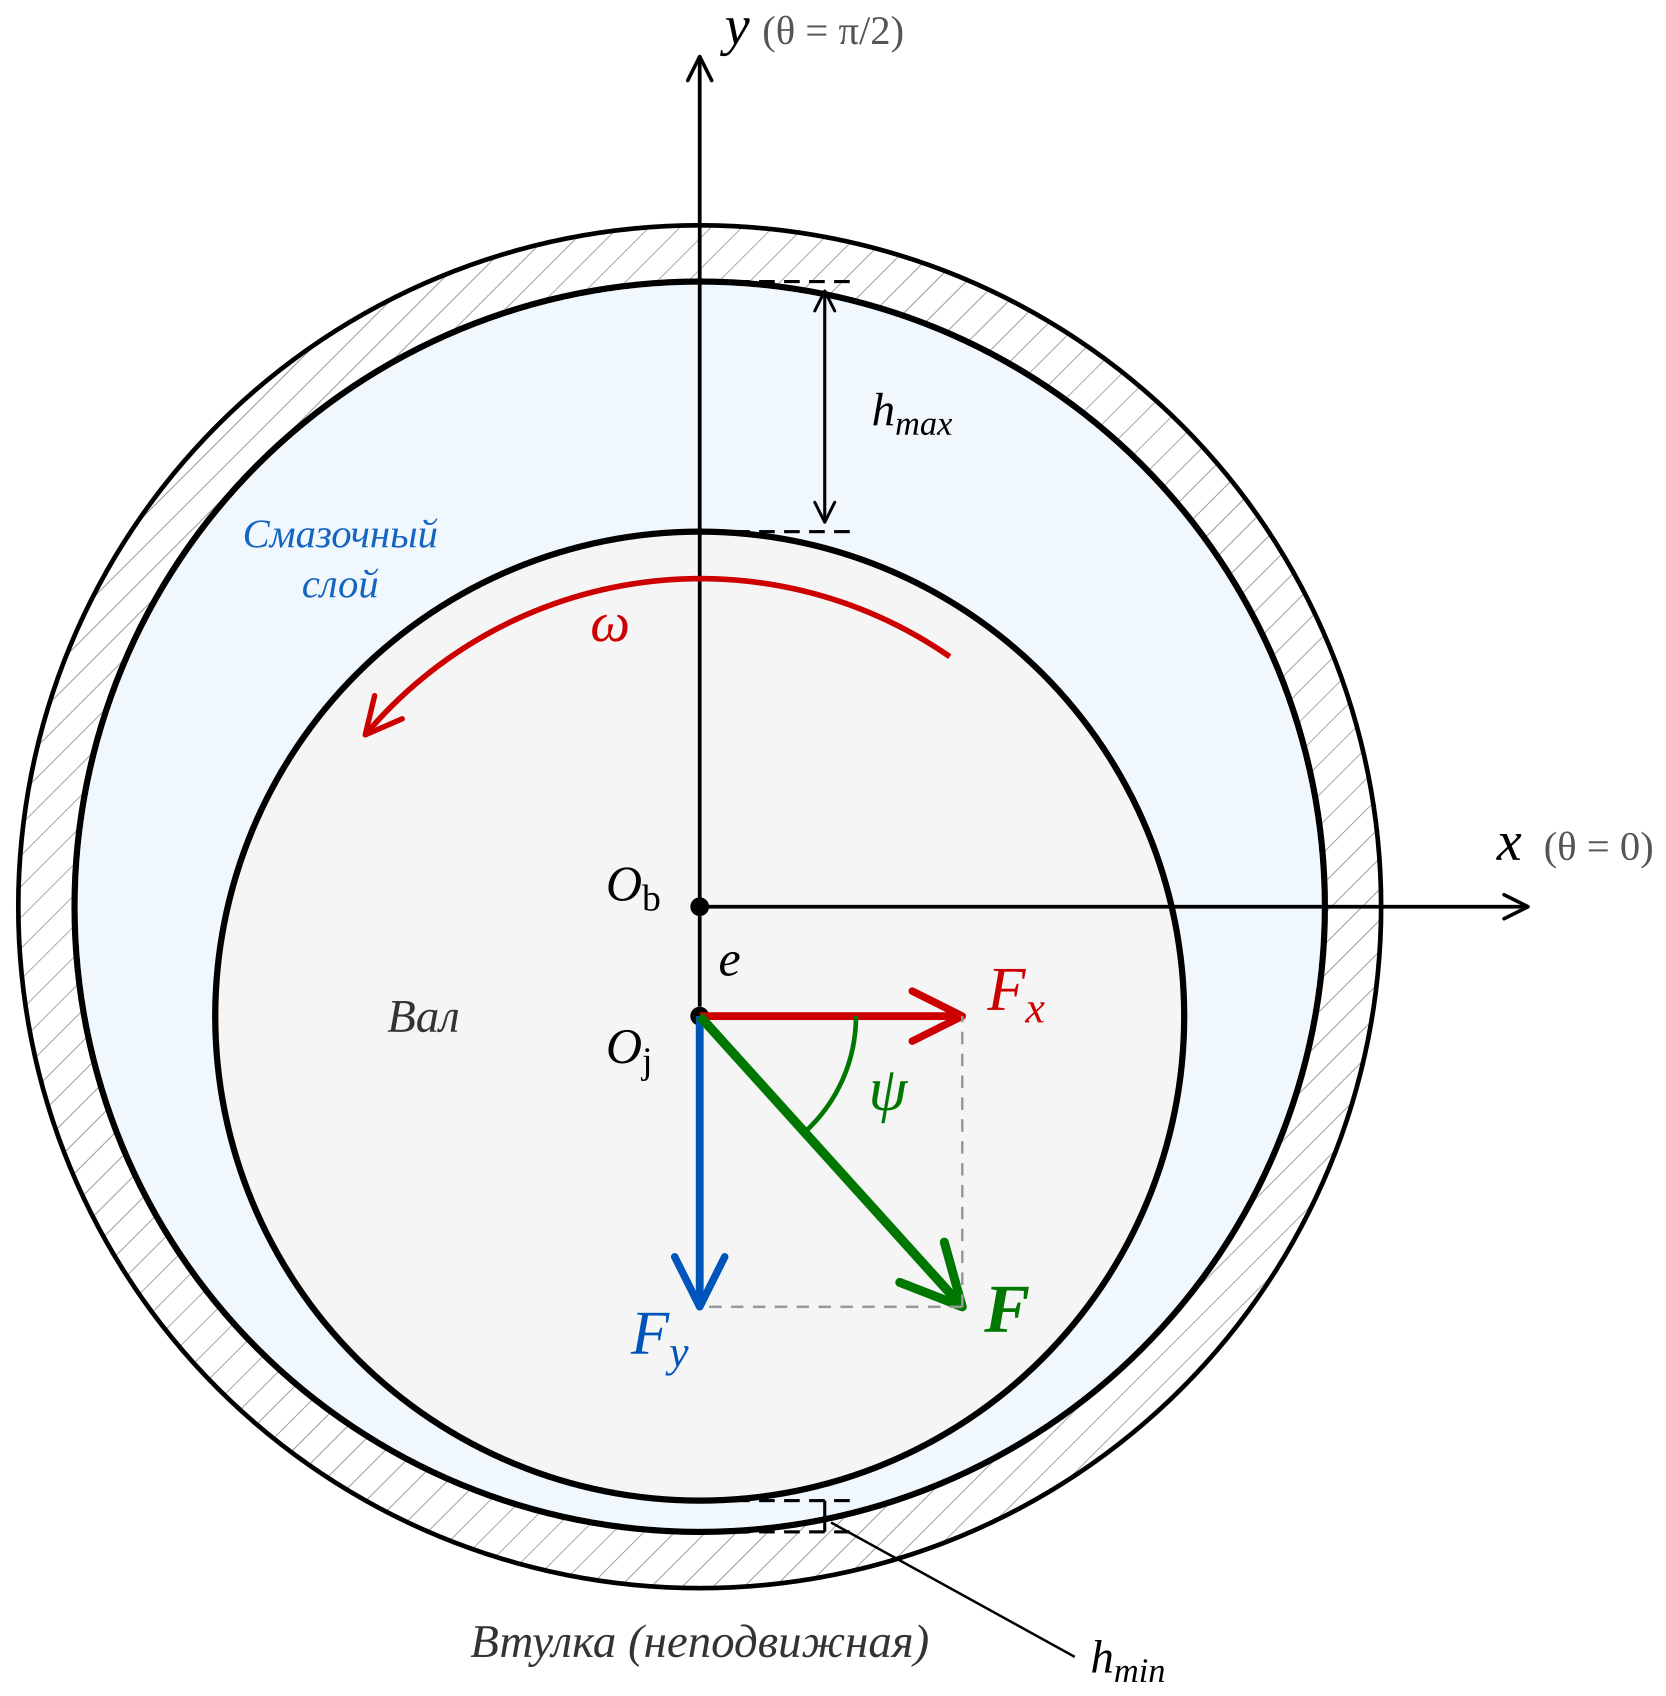
\includegraphics[width=\textwidth,height=0.9\textheight,keepaspectratio]{figures/ch02/fig_2_10.png}
\caption{Компоненты гидродинамической силы на валу/плунжере}
\label{fig:force_components}
\end{figure}

%% ===== Блок 2: Расходы и утечки =====
\subsubsection*{Расходы и утечки}

Удельные потоки $q$ определены в соответствующих постановках
(см.~\eqref{eq:thrust_q_r}, \eqref{eq:journal_q_z},
\eqref{eq:recip_q_z}).
Здесь приводятся только интегральные расходы через границы
рабочей зоны.

Упорный подшипник -- суммарные объёмные расходы через наружную
и внутреннюю кромки (см.~также~\eqref{eq:thrust_Q_radial}):
\begin{equation}
\label{eq:func_Q_thrust}
\begin{split}
  &Q_{\mathrm{out}} = \int_0^{2\pi}
    q_r(R_{\mathrm{out}},\theta)\,R_{\mathrm{out}}\,d\theta, \\
  &Q_{\mathrm{in}} = \int_0^{2\pi}
    q_r(R_{\mathrm{in}},\theta)\,R_{\mathrm{in}}\,d\theta.
\end{split}
\end{equation}

Радиальный подшипник -- утечки через торцы
(см.~также~\eqref{eq:journal_Q_side}):
\begin{equation}
  Q_{\mathrm{out}} = \int_0^{2\pi}
    q_z(\theta,L)\,R\,d\theta,
  \quad
  Q_{\mathrm{in}} = \int_0^{2\pi}
    q_z(\theta,0)\,R\,d\theta.
  \label{eq:func_Q_journal}
\end{equation}

Возвратно-поступательный подшипник -- мгновенные расходы через
обе границы и их усреднение по периоду
(см.~также~\eqref{eq:recip_Q_leakage}):
\begin{equation}
  Q_{\mathrm{out}}(t) = \int_0^{2\pi}
    q_z(\theta,L,t)\,R\,d\theta,
  \quad
  Q_{\mathrm{in}}(t) = \int_0^{2\pi}
    q_z(\theta,0,t)\,R\,d\theta,
  \label{eq:func_Q_recip}
\end{equation}
\begin{equation}
  \langle Q_{\mathrm{out}} \rangle
    = \frac{1}{T}\int_0^T Q_{\mathrm{out}}(t)\,dt,
  \quad
  \langle Q_{\mathrm{in}} \rangle
    = \frac{1}{T}\int_0^T Q_{\mathrm{in}}(t)\,dt,
  \label{eq:func_Q_recip_avg}
\end{equation}
где $T = 2\pi/\Omega$ -- период возвратно-поступательного движения.

Положительный $Q_{\mathrm{out}}$ соответствует вытеканию смазки
из рабочей зоны, что согласуется с конвенцией, принятой
в подразделах~2.1.2-2.1.4.

%% ===== Блок 3: Трение, момент трения, потери мощности =====
\subsubsection*{Сила и момент трения}

Касательное напряжение вдоль направления увлечения $s_1$
следует из профиля скорости~\eqref{eq:velocity_profile_u}.
Первое слагаемое -- вязкое (куэттовское), второе -- давленческое
(пуазейлевское).
Выражения для касательного напряжения на подвижной ($y = h$)
и неподвижной ($y = 0$) поверхностях:
\begin{equation}
  \tau\big|_{y=h} = \frac{\mu\,U}{h}
    + \frac{h}{2}\,\frac{\partial p}{\partial s_1},
  \quad
  \tau\big|_{y=0} = \frac{\mu\,U}{h}
    - \frac{h}{2}\,\frac{\partial p}{\partial s_1}.
  \label{eq:func_tau_both}
\end{equation}

Далее при вычислении момента и силы трения используется напряжение
на неподвижной поверхности $\tau|_{y=0}$, что даёт силу сопротивления
движению.

Конкретизация производной $\partial p/\partial s_1$ и скорости $U$
для каждой постановки:
\begin{itemize}
  \item радиальная: $s_1 = R\theta$ $\Rightarrow$
        $\partial p/\partial s_1 = (1/R)\,\partial p/\partial\theta$,\;
        $U = \omega R$;
  \item упорная: $s_1 = r\theta$ $\Rightarrow$
        $\partial p/\partial s_1 = (1/r)\,\partial p/\partial\theta$,\;
        $U = \omega r$;
  \item возвратно-поступательная: $s_1 = z$ $\Rightarrow$
        $\partial p/\partial s_1 = \partial p/\partial z$,\;
        $U = U(t)$.
\end{itemize}

В приведённых ниже интегралах $\tau$ обозначает касательное
напряжение на неподвижной поверхности $\tau|_{y=0}$.

Момент трения для упорного подшипника:
\begin{equation}
  M_f = \int_0^{2\pi}\!\int_{R_{\mathrm{in}}}^{R_{\mathrm{out}}}
    \tau(r,\theta)\,r^2\,dr\,d\theta.
  \label{eq:func_Mf_thrust}
\end{equation}

Момент трения для радиального подшипника:
\begin{equation}
  M_f = \int_0^L\!\int_0^{2\pi}
    \tau(\theta,z)\,R^2\,d\theta\,dz.
  \label{eq:func_Mf_journal}
\end{equation}

Сила трения для возвратно-поступательного подшипника:
\begin{equation}
  F_f(t) = \int_0^L\!\int_0^{2\pi}
    \tau(\theta,z,t)\,R\,d\theta\,dz.
  \label{eq:func_Ff_recip}
\end{equation}

Потери мощности на трение для вращательных постановок:
\begin{equation}
  P_f = M_f \cdot \omega.
  \label{eq:func_Pf_rot}
\end{equation}

При принятой конвенции (касательное напряжение на неподвижной
поверхности) величины $M_f$ и $F_f$ представляют сопротивление
движению, и потери мощности $P_f \geq 0$.

Для возвратно-поступательной постановки мощность потерь является
функцией времени:
\begin{equation}
  P_f(t) = |F_f(t) \cdot U(t)|,
  \quad
  \langle P_f \rangle = \frac{1}{T}\int_0^T P_f(t)\,dt.
  \label{eq:func_Pf_recip}
\end{equation}

Модуль обеспечивает неотрицательность потерь при смене направления
скорости.

%% ===== Блок 4: Минимальная толщина плёнки =====
\subsubsection*{Минимальная толщина плёнки}

\begin{equation}
  h_{\min}(t) = \min_{(s_1,\,s_2)\,\in\,\Omega}\,h(s_1,s_2,t).
  \label{eq:func_hmin}
\end{equation}

Минимальная толщина плёнки -- критический параметр работоспособности:
при $h_{\min} \to 0$ нарушается режим жидкостного трения.
Для стационарных задач $h_{\min}$ является числом,
для нестационарных -- функцией времени.
Дополнительно может представлять интерес максимальное давление
$p_{\max}(t) = \max_\Omega p$.

%% ===== Блок 5: Коэффициент трения =====
\subsubsection*{Коэффициент трения}

Безразмерный коэффициент трения для радиального
и возвратно-поступательного узлов:
\begin{equation}
  f(t) = \frac{|F_f(t)|}{F(t)}.
  \label{eq:func_f}
\end{equation}

Для упорного подшипника естественнее определять коэффициент трения
через момент:
\begin{equation}
  f_T = \frac{M_f}{W \cdot R_m},
  \quad
  R_m = \frac{R_{\mathrm{in}} + R_{\mathrm{out}}}{2}.
  \label{eq:func_fT}
\end{equation}

%% ===== Завершающий абзац =====

Введённые функционалы определяют основные цели при анализе
и оптимизации подшипников скольжения:
\begin{itemize}
  \item максимизация несущей способности $W$ (или $F$);
  \item минимизация потерь на трение $P_f$ (или $M_f$);
  \item минимизация утечек $Q_{\mathrm{out}}$;
  \item обеспечение $h_{\min}$ выше критического порога
        (предотвращение сухого контакта)~\cite{sfyris2012,chasalevris2012,chasalevris2013}.
\end{itemize}
Для нестационарных задач (подраздел~2.1.4) анализ проводится
как для мгновенных значений, так и для усреднённых по периоду
$\langle \cdot \rangle$.


\FloatBarrier
\section{Модель с детерминированными микроструктурами}
\subsection{Параметризация микрорельефа}

В разделе~2.1 рассмотрены постановки задачи смазки для гладких
поверхностей. Для учёта детерминированных микроструктур необходимо
задать модификацию функции зазора~$h$, описывающую геометрию
нанесённых на поверхность элементов. Настоящий подраздел вводит общую
параметрическую модель микрорельефа, используемую далее
в~2.2.2-2.2.4. Формулы записываются для произвольных поверхностных
координат; конкретные координаты определяются постановкой
(таблица~\ref{tab:nondim_scales} в подразделе~2.1.6).

%% ===== Блок 1: Суперпозиция =====

\subsubsection*{Суперпозиция зазора}

Рабочую поверхность представляем в виде гладкой базовой поверхности
с наложенными регулярными элементами. Суммарная толщина смазочного
слоя записывается как суперпозиция базового зазора и добавки,
описывающей микрорельеф:
\begin{equation}
  h(x_1, x_2)
    = h_{\mathrm{base}}(x_1, x_2) + \Delta h(x_1, x_2),
  \label{eq:h_superposition}
\end{equation}
где $(x_1, x_2)$ -- поверхностные координаты с размерностью длины.
В зависимости от постановки:
\begin{itemize}
  \item радиальный подшипник: $x_1 = R\theta$, $x_2 = z$;
  \item возвратно-поступательная постановка: $x_1 = z$,
        $x_2 = R\theta$;
  \item упорный подшипник: $x_1 = R\theta$, $x_2 = r$,
\end{itemize}
где $R$ -- характерный радиус (подраздел~2.1.6). Для упорного
подшипника дуговая координата по окружному направлению в общем случае
равна $r\theta$; здесь используется аппроксимация $x_1 = R\theta$
с характерным (например, средним) радиусом, что удобно для
унифицированного задания микрорельефа и раскладки.

Слагаемые в~\eqref{eq:h_superposition} имеют следующий смысл:
\begin{itemize}
  \item $h_{\mathrm{base}}$ -- толщина зазора для гладкой поверхности,
        определённая в подразделах~2.1.2-2.1.4;
  \item $\Delta h$ -- локальная добавка, описывающая микрорельеф.
\end{itemize}
Знаковая конвенция: $\Delta h \geq 0$ для углублений (лунок),
$\Delta h \leq 0$ для выступов. Принцип суперпозиции проиллюстрирован
на рисунке~\ref{fig:h_superposition}.

% [РИСУНОК: Суперпозиция зазора h = h_base + Δh]
% Должен показывать два вида:
% (1) Продольный разрез: базовый клин h_base + ямка Δh → суммарный h
% (2) Вид сверху: пятно одного элемента микроструктуры на фоне сектора
\begin{figure}[!ht]
\centering
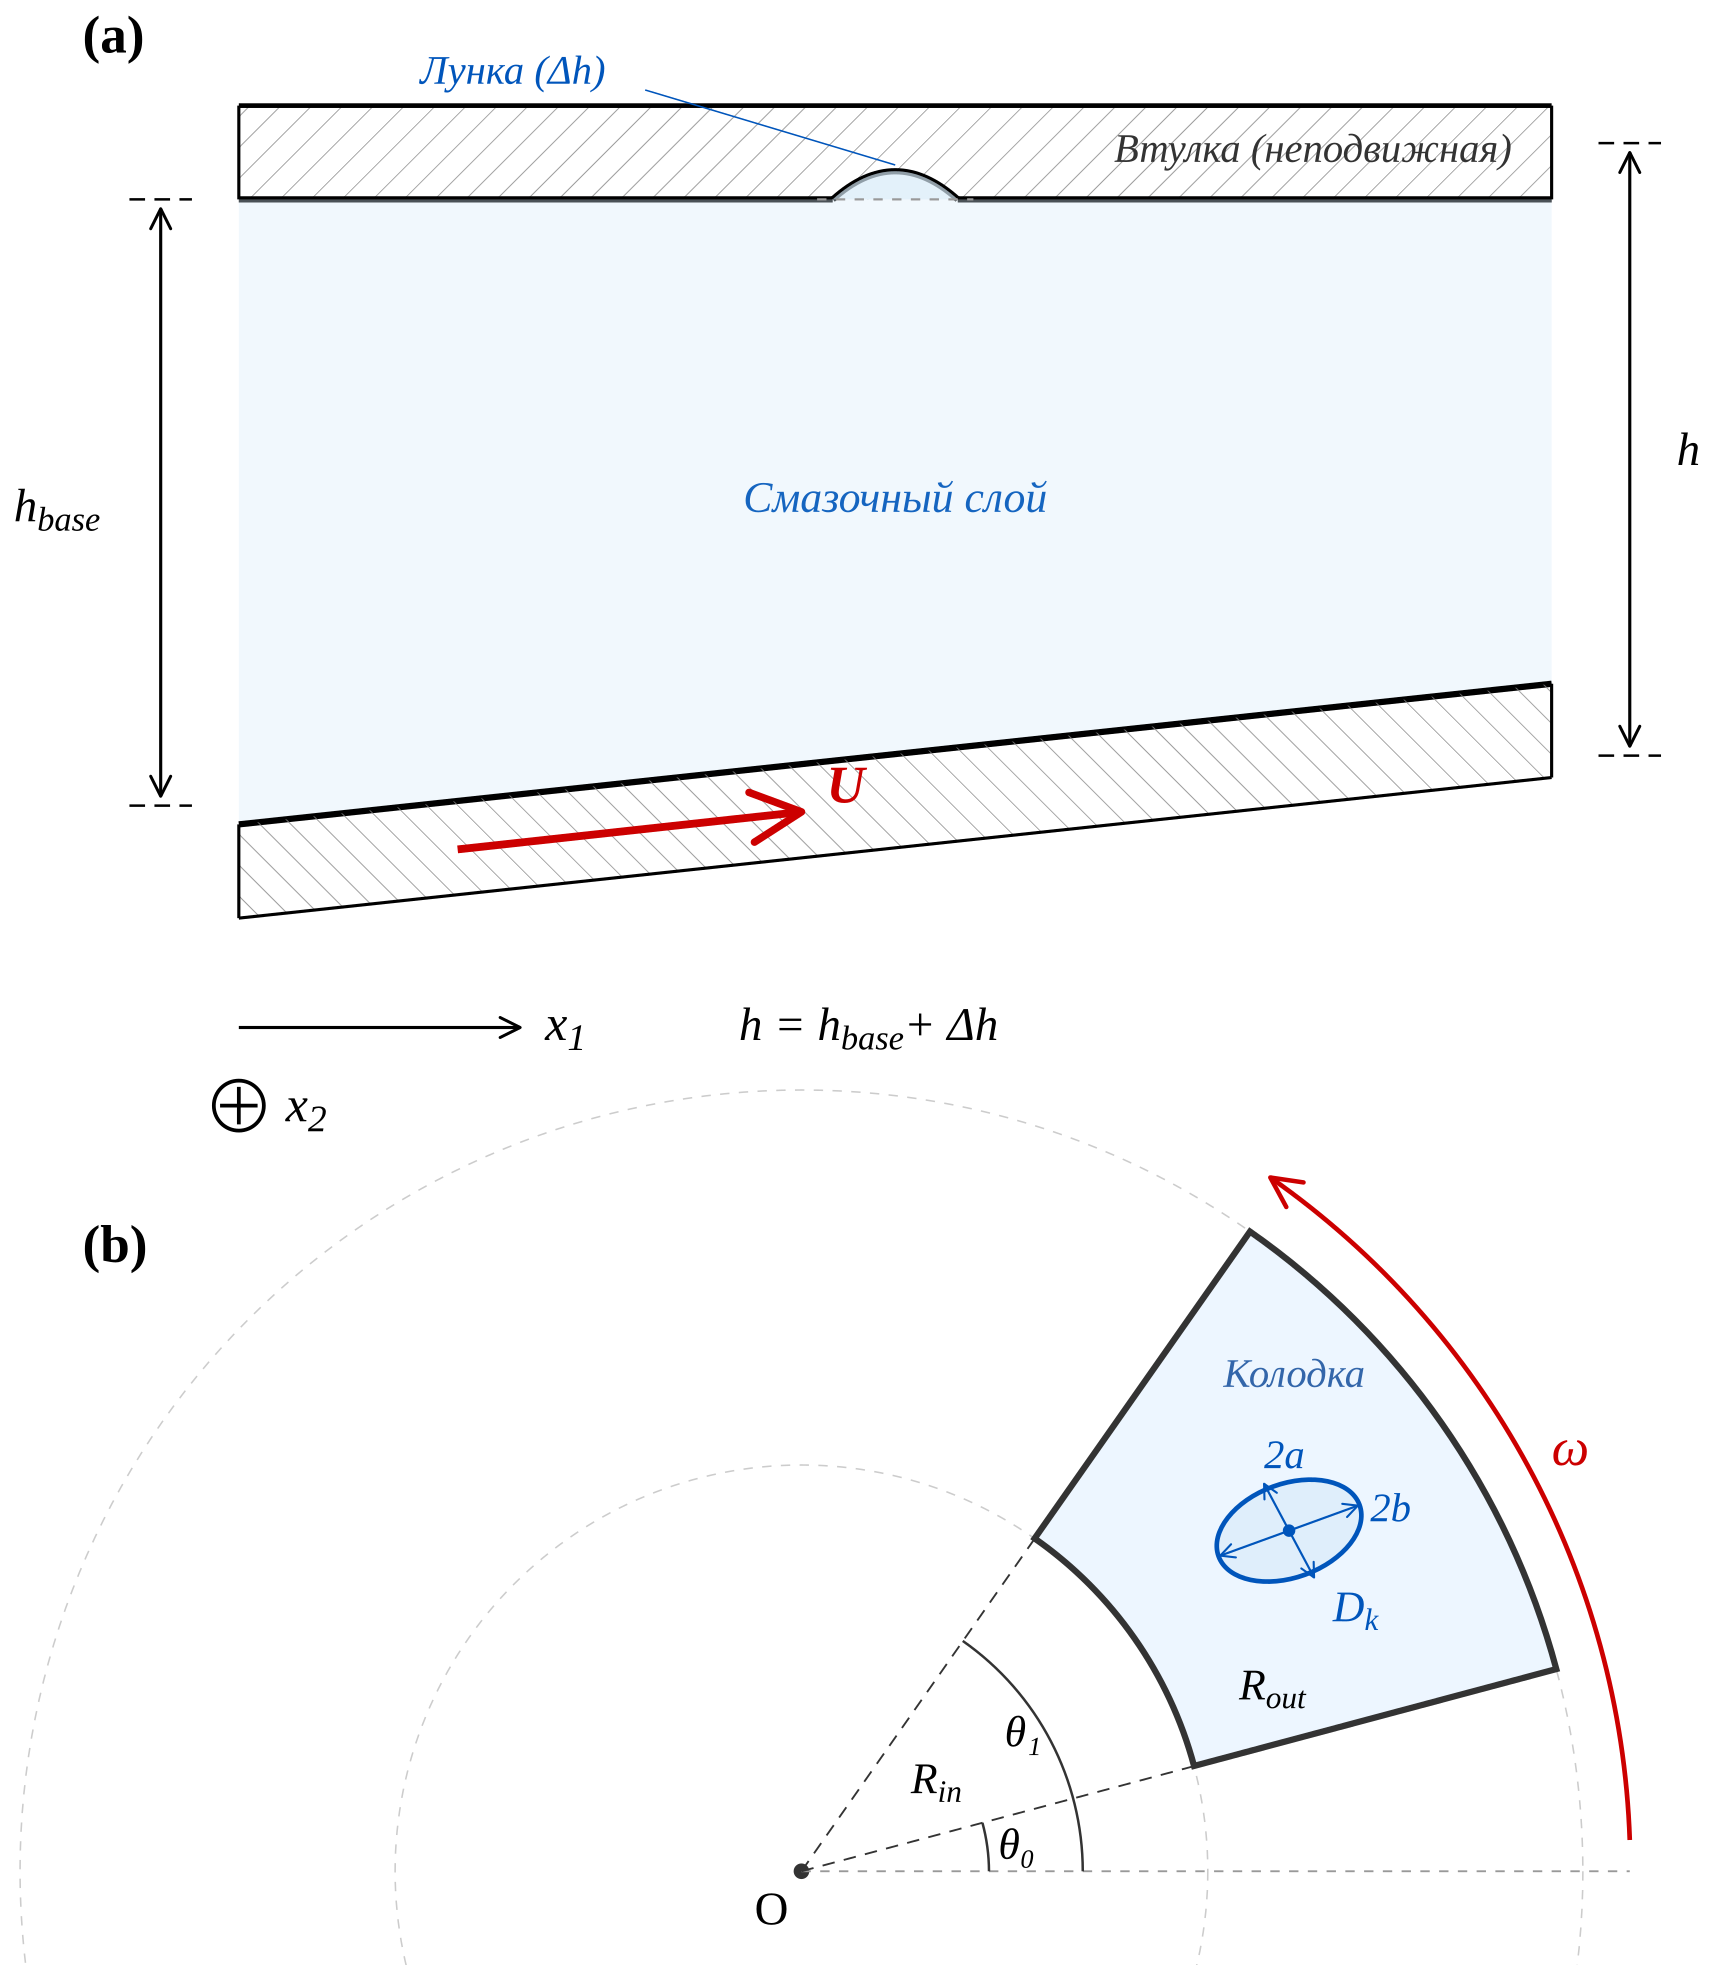
\includegraphics[width=\textwidth,height=0.9\textheight,keepaspectratio]{figures/ch02/fig_2_11.png}
\caption{Суперпозиция толщины зазора: базовый профиль и локальная
  микроструктура}
\label{fig:h_superposition}
\end{figure}

%% ===== Блок 2: Сумма вкладов =====

\subsubsection*{Представление микрорельефа}

Микрорельеф представляется набором из~$N$ локализованных элементов,
вклады которых суммируются:
\begin{equation}
  \Delta h(x_1, x_2)
    = \sum_{k=1}^{N} \Delta h_k(x_1, x_2).
  \label{eq:delta_h_sum}
\end{equation}

Каждый элемент задаётся общим шаблоном (конкретный вид профиля
определяется в подразделе~2.2.2):
\begin{equation}
  \Delta h_k(x_1, x_2)
    = \begin{cases}
        \sigma_k\, h_{p,k}\,
          f_k(x_1 - x_{1,k},\; x_2 - x_{2,k}),
          & (x_1, x_2) \in D_k, \\
        0,
          & (x_1, x_2) \notin D_k,
      \end{cases}
  \label{eq:delta_h_element}
\end{equation}
где:
\begin{itemize}
  \item $D_k$ -- область поддержки (пятно) $k$-го элемента
        на поверхности;
  \item $f_k$ -- профильная функция, задающая форму элемента;
        $f_k(0,0) = 1$;
  \item $\sigma_k = +1$ для углублений (лунок),
        $\sigma_k = -1$ для выступов;
  \item $h_{p,k}$ -- глубина (высота) элемента;
  \item $(x_{1,k},\, x_{2,k})$ -- координаты центра $k$-го элемента.
\end{itemize}

При наличии периодичности по координате $x_1$ (или $x_2$) разность
$x_1 - x_{1,k}$ понимается как минимальная по модулю с учётом
периода~$L_1$ (например, $L_1 = 2\pi R$ для окружного направления).

\paragraph{Эллиптические элементы.}
Для осесимметричных и эллиптических лунок удобно параметризовать
область элемента через безразмерную радиальную координату:
\begin{equation}
  \rho_k
    = \sqrt{
        \left(\frac{x_1 - x_{1,k}}{b_k}\right)^{\!2}
      + \left(\frac{x_2 - x_{2,k}}{a_k}\right)^{\!2}
      }.
  \label{eq:rho_k}
\end{equation}

Тогда $D_k = \{\rho_k \leq 1\}$ -- эллипс с полуосями $b_k$ по~$x_1$
и~$a_k$ по~$x_2$, а профильная функция зависит только от~$\rho$:
$f_k = f(\rho_k)$, причём $f(0) = 1$, $f(1) = 0$.

Для канавок и других неосесимметричных элементов область~$D_k$
и профильная функция~$f_k$ задаются иначе; конкретные формы
рассматриваются в подразделе~2.2.2.

Для однородной текстуры все элементы идентичны
($a_k = a$, $b_k = b$, $h_{p,k} = h_p$, $f_k = f$) и различаются
только положением центров. Типовой элемент с основными обозначениями показан на рис.~\ref{fig:microtexture_params}.

% [РИСУНОК 2.5: Типовая микроструктура с параметрами]
\begin{figure}[!ht]
\centering
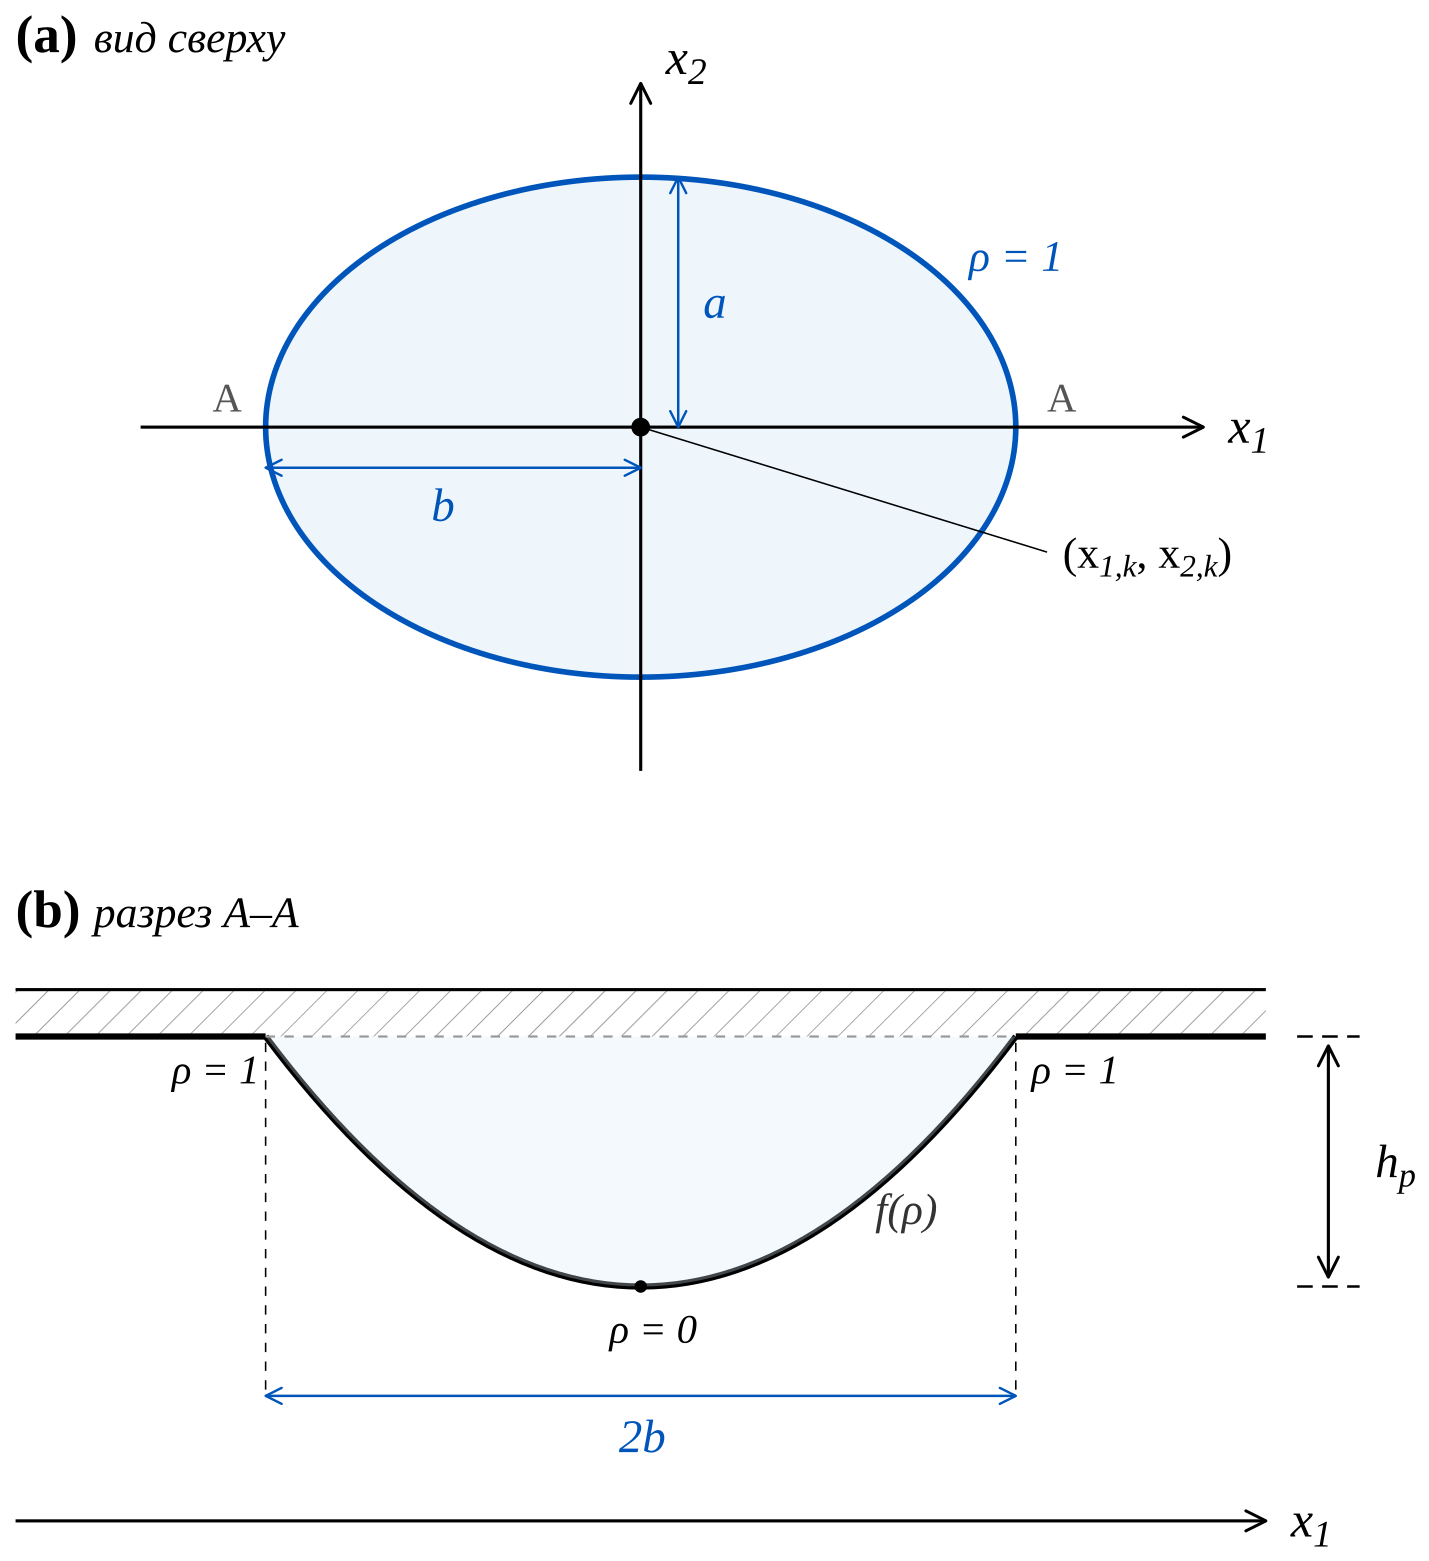
\includegraphics[width=\textwidth,height=0.9\textheight,keepaspectratio]{figures/ch02/fig_2_12.png}
\caption{Типовой элемент микроструктуры с основными геометрическими
  параметрами}
\label{fig:microtexture_params}
\end{figure}

%% ===== Блок 3: Параметры раскладки =====

\subsubsection*{Параметры раскладки}

Положение элементов на поверхности определяется раскладкой. Для её
описания вводятся следующие параметры:
\begin{itemize}
  \item $p_1$, $p_2$ -- шаги раскладки, т.\,е. расстояния между
        центрами соседних элементов по направлениям $x_1$ и~$x_2$;
  \item $N$ -- общее число элементов;
  \item область текстурирования -- участок поверхности, на который
        нанесена текстура (может совпадать со всей расчётной областью
        или быть её частью).
\end{itemize}

Важной интегральной характеристикой является коэффициент заполнения --
доля площади поверхности, занятая элементами:
\begin{equation}
  \phi = \frac{N \cdot A_{\mathrm{elem}}}{A_{\mathrm{tex}}},
  \label{eq:fill_fraction}
\end{equation}
\begin{conditions}
$A_{\mathrm{elem}}$ -- площадь «пятна» одного элемента (для
эллипса $A_{\mathrm{elem}} = \pi a b$);\\
$A_{\mathrm{tex}}$ -- площадь области текстурирования.
\end{conditions}
Конкретные типы решёток (прямоугольная, шахматная, гексагональная
и~др.) и способы задания координат центров рассматриваются
в подразделе~2.2.3.

%% ===== Блок 4: Ограничения модели =====

\subsubsection*{Ограничения модели}

Введённая параметризация корректна при выполнении следующих условий.
\begin{enumerate}
  \item Положительность зазора: $h(x_1, x_2) > 0$ на всей расчётной
        области. Формально:
        $h_{\mathrm{base}}(x_1, x_2) + \Delta h(x_1, x_2) > 0$.
        В частности, при непересекающихся одинаковых лунках достаточно
        $h_p < h_{\mathrm{base,min}}$.
  \item Непересечение элементов:
        $D_k \cap D_{k'} = \varnothing$ для всех $k \neq k'$.
        Для эллиптических элементов без поворота достаточное условие:
        $p_1 \geq 2b$, $p_2 \geq 2a$.
  \item Малая глубина: $h_p / h_0 \ll 1$ обеспечивает применимость
        уравнения Рейнольдса к текстурированной поверхности
        (см.\ подраздел~2.1.5).
  \item Гладкость профиля: непрерывность $\Delta h$ на границе
        элемента ($f(1) = 0$). Желательна также гладкая стыковка
        ($f'(1) = 0$) для уменьшения численных артефактов. Выполнение
        этих условий зависит от выбора профильной функции~$f(\rho)$
        (подраздел~2.2.2).
\end{enumerate}

%% ===== Блок 5: Таблица параметров =====

Полный перечень параметров микроструктуры приведён в табл.~\ref{tab:texture_params}.

\begin{table}[!ht]
\centering
\caption{Параметры детерминированной микроструктуры}
\label{tab:texture_params}
\begin{tabularx}{\textwidth}{|X|c|c|}
\hline
\multicolumn{1}{|c|}{\textbf{Параметр}} & \textbf{Обозначение} & \textbf{Размерность} \\
\hline
Глубина (высота) элемента & $h_p$     & мкм \\
\hline
Полуось по $x_1$ (эллиптич.) & $b$    & мкм \\
\hline
Полуось по $x_2$ (эллиптич.) & $a$    & мкм \\
\hline
Шаг по $x_1$              & $p_1$     & мкм \\
\hline
Шаг по $x_2$              & $p_2$     & мкм \\
\hline
Число элементов           & $N$       & --  \\
\hline
Доля площади (заполнение) & $\phi$    & --  \\
\hline
Профильная функция        & $f(\rho)$ & --  \\
\hline
\end{tabularx}
\end{table}

%% ===== Завершающий абзац =====

Введённая параметрическая модель позволяет описать широкий класс
детерминированных микроструктур~\cite{senatore2018,joshi2018}. Конкретные формы профильной
функции~$f(\rho)$ рассматриваются в подразделе~2.2.2, типы
раскладок -- в подразделе~2.2.3, а переход к безразмерным
параметрам -- в подразделе~2.2.4.

\FloatBarrier
\subsection{Форма микроструктур}

В подразделе~2.2.1 введён общий шаблон элемента микрорельефа:
$\Delta h_k = \sigma_k\, h_{p}\, f_k(\ldots)$ на области~$D_k$.
Цель настоящего подраздела -- задать конкретные профильные
функции~$f$ и формы областей~$D_k$ для всех типов элементов,
используемых в работе. Общие требования к профильной функции
формулируются следующим образом:
\begin{itemize}
  \item $f(0,0) = 1$ (или $f(0) = 1$ для осесимметричных элементов);
  \item $f = 0$ на границе~$D_k$;
  \item желательна непрерывность~$f$ и гладкая стыковка на границе:
        для профилей вида $f(\rho)$ -- $df/d\rho|_{\rho=1} = 0$,
        в общем случае -- $\partial f/\partial n = 0$ на~$\partial D_k$
        (где $n$ -- внешняя нормаль);
  \item $0 \leq f \leq 1$ внутри~$D_k$.
\end{itemize}

%% ===== Блок 1: Локальные координаты =====

\subsubsection*{Локальные координаты элемента}

Для описания элементов произвольной ориентации вводятся локальные
координаты $(\xi, \eta)$, связанные с глобальными $(x_1, x_2)$
поворотом на угол~$\alpha_k$:
\begin{equation}
  \begin{alignedat}{2}
    & \xi  &\;=\;& \phantom{-}(x_1 - x_{1,k})\cos\alpha_k
            + (x_2 - x_{2,k})\sin\alpha_k, \\
    & \eta &\;=\;& -(x_1 - x_{1,k})\sin\alpha_k
            + (x_2 - x_{2,k})\cos\alpha_k.
  \end{alignedat}
  \label{eq:local_coords}
\end{equation}

При $\alpha_k = 0$ локальные координаты совпадают с глобальными. Взаимное расположение осей иллюстрирует рис.~\ref{fig:local_coords}.

Безразмерная радиальная координата для эллиптических элементов
(введённая в подразделе~2.2.1) записывается через локальные
координаты:
\begin{equation}
  \rho_k = \sqrt{\left(\frac{\xi}{b_k}\right)^{\!2}
              +\left(\frac{\eta\vphantom{\xi}}{a_k}\right)^{\!2}}.
  \label{eq:rho_local}
\end{equation}

Область элемента: $D_k = \{\rho_k \leq 1\}$. Для канавок
и прямоугольных элементов область~$D_k$ задаётся иначе (см.\ ниже).

% [РИСУНОК: Локальные координаты элемента]
\begin{figure}[!ht]
\centering
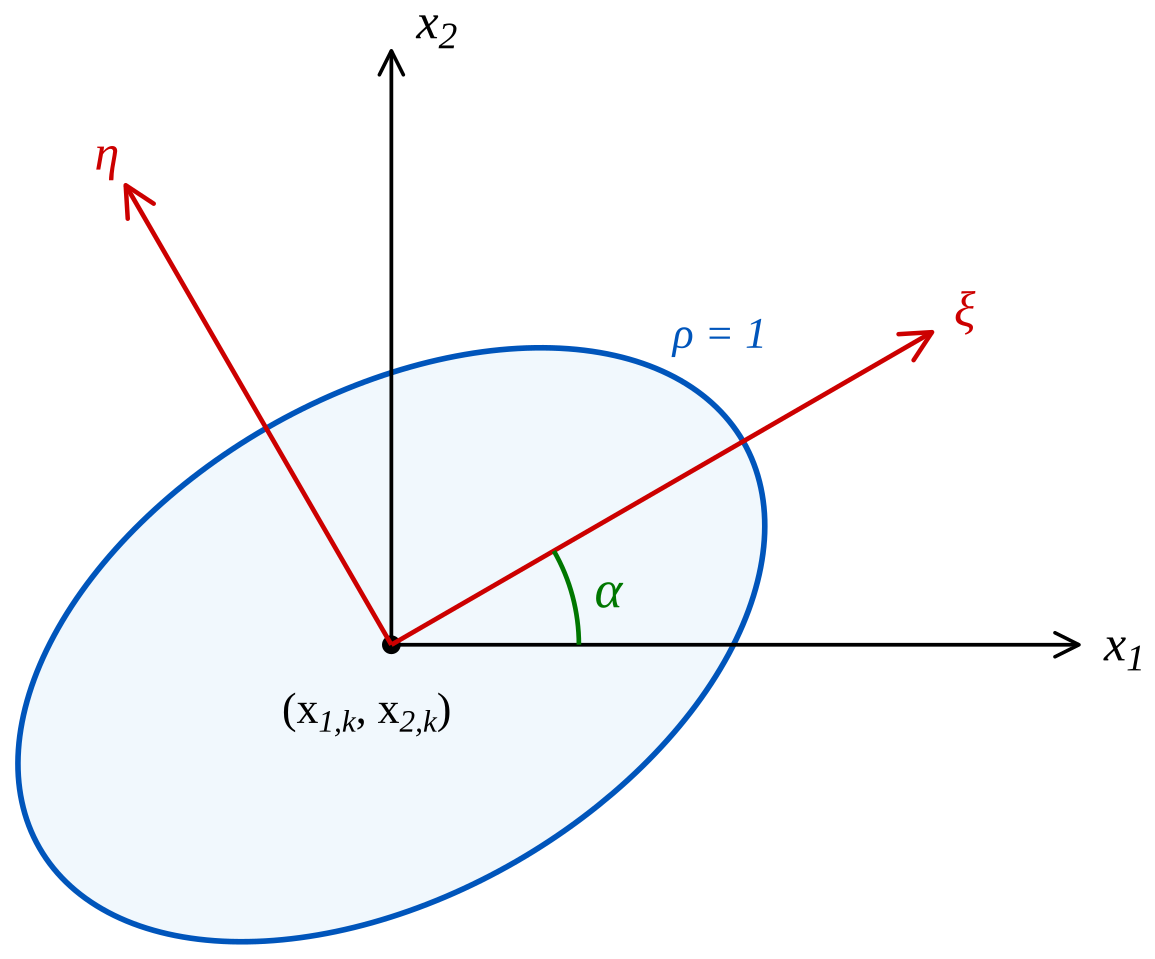
\includegraphics[width=\textwidth,height=0.9\textheight,keepaspectratio]{figures/ch02/fig_2_13.png}
\caption{Локальные координаты элемента микроструктуры и угол поворота}
\label{fig:local_coords}
\end{figure}

%% ===== Блок 2: Осесимметричные и эллиптические профили =====

\subsubsection*{Осесимметричные и эллиптические элементы}

Для элементов с эллиптической областью $D_k = \{\rho_k \leq 1\}$
профильная функция зависит только от~$\rho_k$ (далее для краткости
$\rho$). Ниже приведены основные типы профилей.

\paragraph{A) Эллипсоидальный (полусфероидальная шапка).}
\begin{equation}
  f(\rho) = \sqrt{1 - \rho^2}.
  \label{eq:profile_ellipsoidal}
\end{equation}

Свойства: $f(1) = 0$, но $f'(1) \to -\infty$ (вертикальный обрыв
на границе). При $a = b$ профиль соответствует полусфере. Широко
используется в литературе; на практике разрыв производной обычно
не вызывает проблем при достаточном разрешении сетки.

\paragraph{B) Параболический.}
\begin{equation}
  f(\rho) = 1 - \rho^2.
  \label{eq:profile_parabolic}
\end{equation}

Свойства: $f(1) = 0$, $f'(1) = -2 \neq 0$. Простейший гладкий
профиль. При $a = b$ -- параболоид вращения.

\paragraph{C) Конический (линейный).}
\begin{equation}
  f(\rho) = 1 - \rho.
  \label{eq:profile_conical}
\end{equation}

Свойства: $f(1) = 0$, $df/d\rho|_{\rho=1} = -1$. Как функция
от~$(\xi, \eta)$ через~$\rho$ имеет недифференцируемость в центре
($\rho = 0$), что может приводить к численным артефактам на грубых
сетках.

\paragraph{D) Косинусный.}
\begin{equation}
  f(\rho) = \tfrac{1}{2}\bigl(1 + \cos(\pi\rho)\bigr).
  \label{eq:profile_cosine}
\end{equation}

Свойства: $f(1) = 0$, $f'(1) = 0$. Обеспечивает гладкую стыковку
на границе элемента. Предпочтителен для численных расчётов.

\paragraph{E) Полиномиальный (smoothstep).}
\begin{equation}
  f(\rho) = 1 - 3\rho^2 + 2\rho^3.
  \label{eq:profile_smoothstep}
\end{equation}

Свойства: $f(1) = 0$, $f'(1) = 0$, $f'(0) = 0$. Двусторонняя
гладкость -- и в центре, и на границе.

\paragraph{F) Цилиндрический (плоское дно).}
Вводится параметр $\rho_0$ ($0 < \rho_0 < 1$) -- радиус плоского
участка:
\begin{equation}
  f(\rho) =
    \begin{cases}
      1,
        & 0 \leq \rho \leq \rho_0, \\[4pt]
      g\!\left(\dfrac{\rho - \rho_0}{1 - \rho_0}\right),
        & \rho_0 < \rho \leq 1,
    \end{cases}
  \label{eq:profile_plateau}
\end{equation}
где $g(t)$ -- функция перехода от~1 к~0 на отрезке $t \in [0,\,1]$.
Общие требования: $g(0) = 1$, $g(1) = 0$; для гладкой стыковки
на внешней границе дополнительно $g'(1) = 0$ (и желательно
$g'(0) = 0$, что обеспечивает плавный переход от плоского участка
к наклонной стенке).
Примеры: $g(t) = 1 - t^2$ (параболический переход, без гладкой
стыковки по наклону),
$g(t) = \frac{1}{2}(1 + \cos\pi t)$ (гладкий косинусный переход).

При $\rho_0 \to 0$ профиль вырождается в соответствующий «обычный»
тип; при $\rho_0 \to 1$ -- приближается к цилиндрическому с резкими
стенками. Параметр~$\rho_0$ позволяет моделировать лунки с плоским
дном, характерные для лазерного текстурирования. При $a = b$ и без
функции перехода ($g$ -- ступенька) элемент представляет собой
круговой цилиндр; при $a \neq b$ -- эллиптический цилиндр.

%% ===== Блок 3: Канавки =====

\subsubsection*{Канавки}

Для канавок область~$D_k$ -- прямоугольник в локальных координатах:
\begin{equation}
  D_k = \bigl\{|\xi| \leq \ell/2,\; |\eta| \leq a\bigr\},
  \label{eq:groove_Dk}
\end{equation}
\begin{conditions}
$\ell$ -- длина канавки (вдоль~$\xi$);\\
$a$ -- полуширина (по~$\eta$).
\end{conditions}
Профильная функция задаётся по поперечному направлению~$\eta$
(вдоль~$\xi$ профиль постоянен):
\begin{equation}
  f_k(\xi, \eta) = f_\perp\!\bigl(|\eta|/a\bigr),
  \label{eq:groove_profile}
\end{equation}
где $f_\perp(t)$, $t \in [0,\,1]$ -- поперечный профиль.

При необходимости гладкого замыкания канавки по концам вводится
продольное окно:
\begin{equation}
  f_k(\xi, \eta)
    = f_\parallel\!\bigl(|\xi|/(\ell/2)\bigr)
      \cdot f_\perp\!\bigl(|\eta|/a\bigr),
  \label{eq:groove_profile_window}
\end{equation}
где $f_\parallel(s)$, $s \in [0,\,1]$ -- продольный профиль
с условиями $f_\parallel(0) = 1$, $f_\parallel(1) = 0$. Например,
$f_\parallel(s) = \frac{1}{2}(1 + \cos\pi s)$. Для канавок
с резкими торцами полагают $f_\parallel \equiv 1$.

Примеры поперечного профиля:
параболический $f_\perp(t) = 1 - t^2$,
косинусный $f_\perp(t) = \frac{1}{2}(1 + \cos\pi t)$,
прямоугольный $f_\perp(t) = 1$.
Прямоугольный профиль $f_\perp(t) = 1$ соответствует ступенчатому
разрыву на границе элемента и используется для моделирования канавок
с резкими стенками; при необходимости гладкой стыковки следует
выбирать $f_\perp(1) = 0$.

Ориентация канавки задаётся углом~$\alpha_k$ через формулы локальных
координат~\eqref{eq:local_coords}. При $\alpha_k = 0$ канавка
ориентирована вдоль~$x_1$ (продольная), при $\alpha_k = \pi/2$ --
вдоль~$x_2$ (поперечная). Дополнительным параметром канавки является
её длина~$\ell$.

%% ===== Блок 4: Сводная таблица =====

\subsubsection*{Сводка типов профилей}

Основные типы профильных функций и их свойства приведены
в таблице~\ref{tab:profile_types}; сравнение форм профилей показано на рис.~\ref{fig:profile_comparison}, а общий вид элементов -- на рис.~\ref{fig:texture_geometries}.

\begin{table}[!ht]
\centering
\caption{Типы профильных функций элементов микрорельефа}
\label{tab:profile_types}
\small
\begin{tabular}{|p{3.0cm}|c|c|c|p{3.8cm}|}
\hline
\textbf{Тип} & \textbf{Профильная функция}
  & $\boldsymbol{f(1){=}0}$ & $\boldsymbol{df/d\rho|_{1}{=}0}$
  & \textbf{Комментарий} \\
\hline
Эллипсоидальный & $\sqrt{1-\rho^2}$
  & да & нет & $f' \to -\infty$ на границе \\
\hline
Параболический & $1-\rho^2$
  & да & нет & простейший гладкий \\
\hline
Конический & $1-\rho$
  & да & нет & излом в центре \\
\hline
Косинусный & $\frac{1}{2}(1+\cos\pi\rho)$
  & да & да & гладкая стыковка \\
\hline
Smoothstep & $1-3\rho^2+2\rho^3$
  & да & да & гладкость с~обеих сторон \\
\hline
Плоское дно & кусочная (см.\ текст)
  & да & зависит от~$g$ & лазерные лунки \\
\hline
Канавка & $f_\perp(|\eta|/a)$
  & -- & -- & профиль по~$\eta$ \\
\hline
\end{tabular}
\end{table}

%% ===== Блок 5: Рисунки =====

% [РИСУНОК: Сравнение профилей f(ρ)]
\begin{figure}[!ht]
\centering
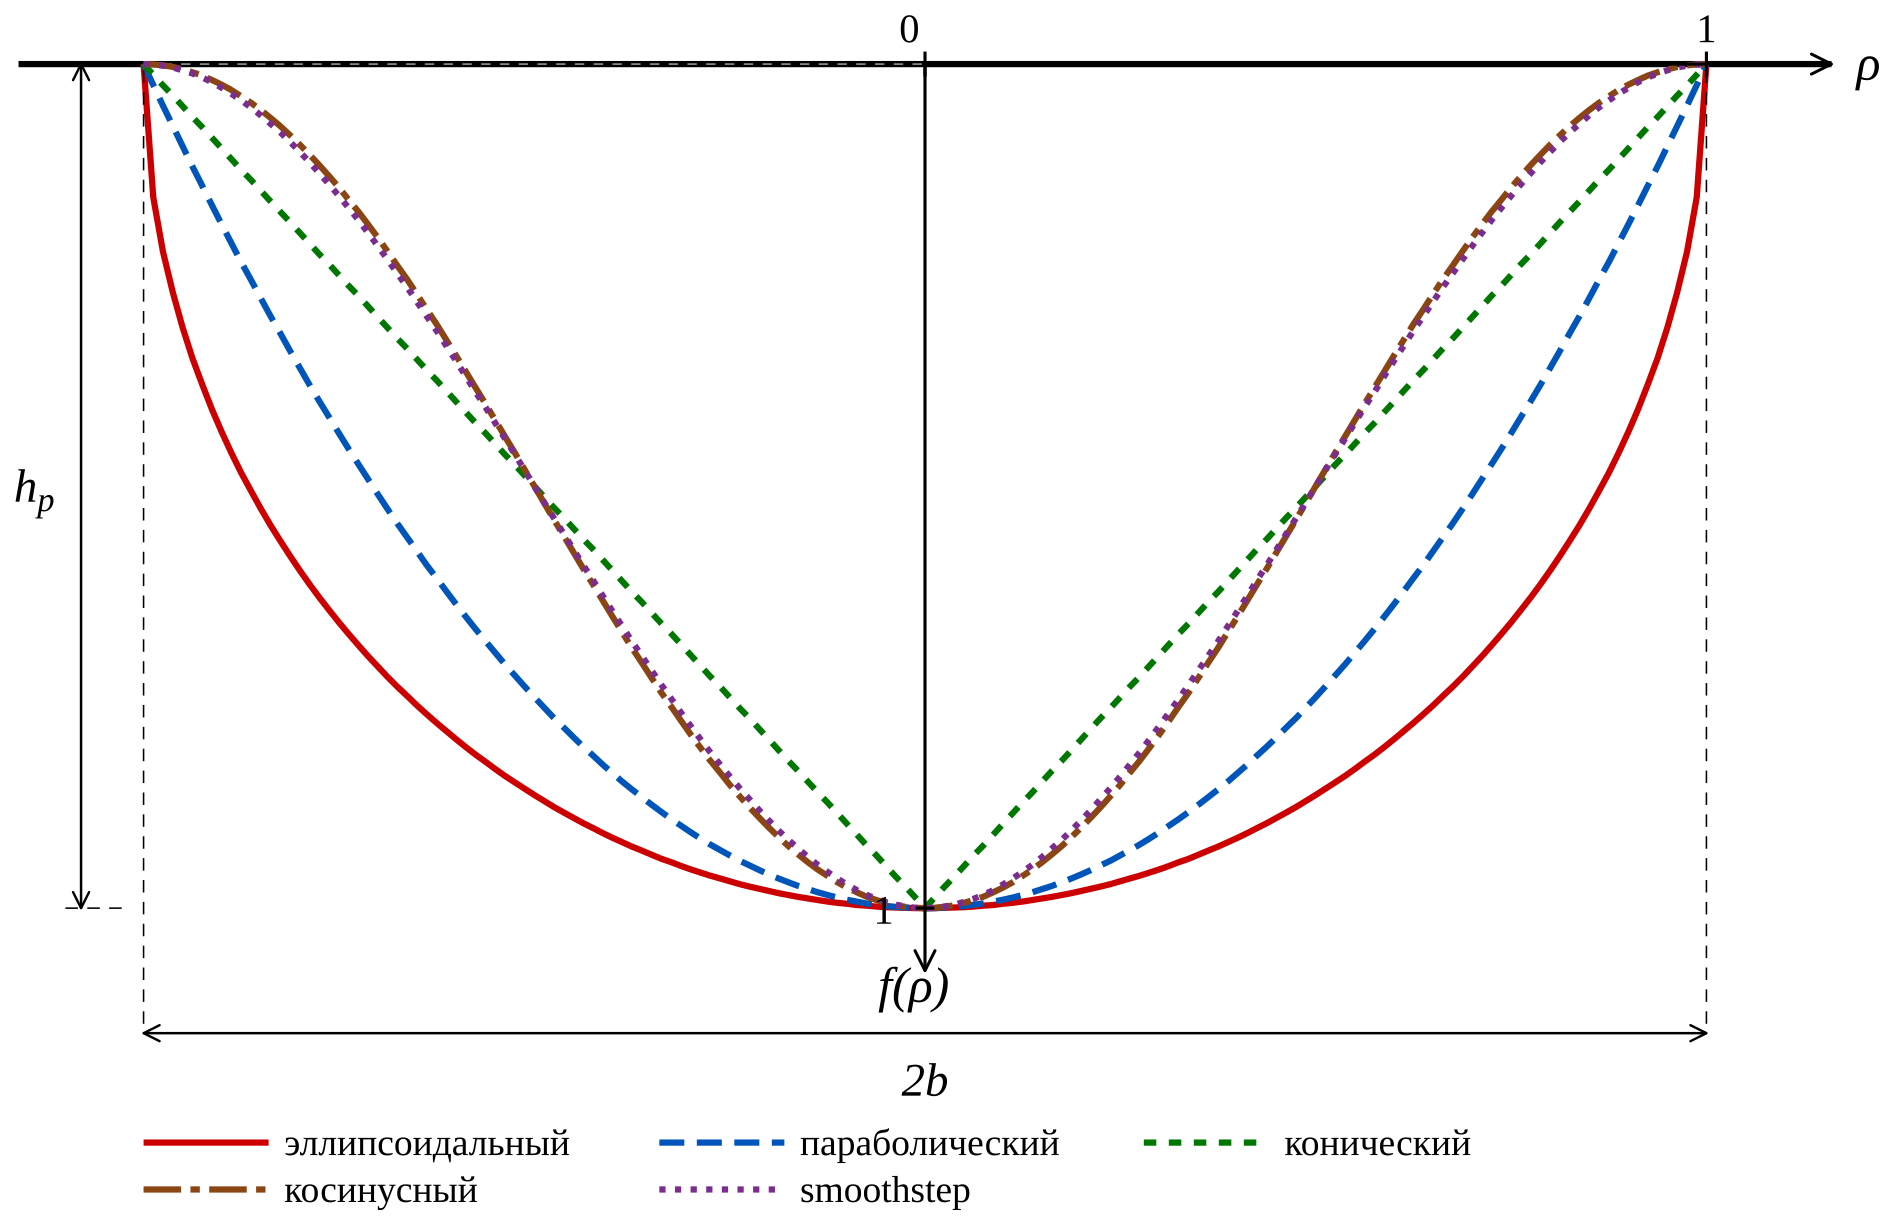
\includegraphics[width=\textwidth,height=0.9\textheight,keepaspectratio]{figures/ch02/fig_2_14.png}
\caption{Сравнение профильных функций элементов микрорельефа}
\label{fig:profile_comparison}
\end{figure}

% [РИСУНОК: Типы микроструктур (обновлённый)]
\begin{figure}[!ht]
\centering
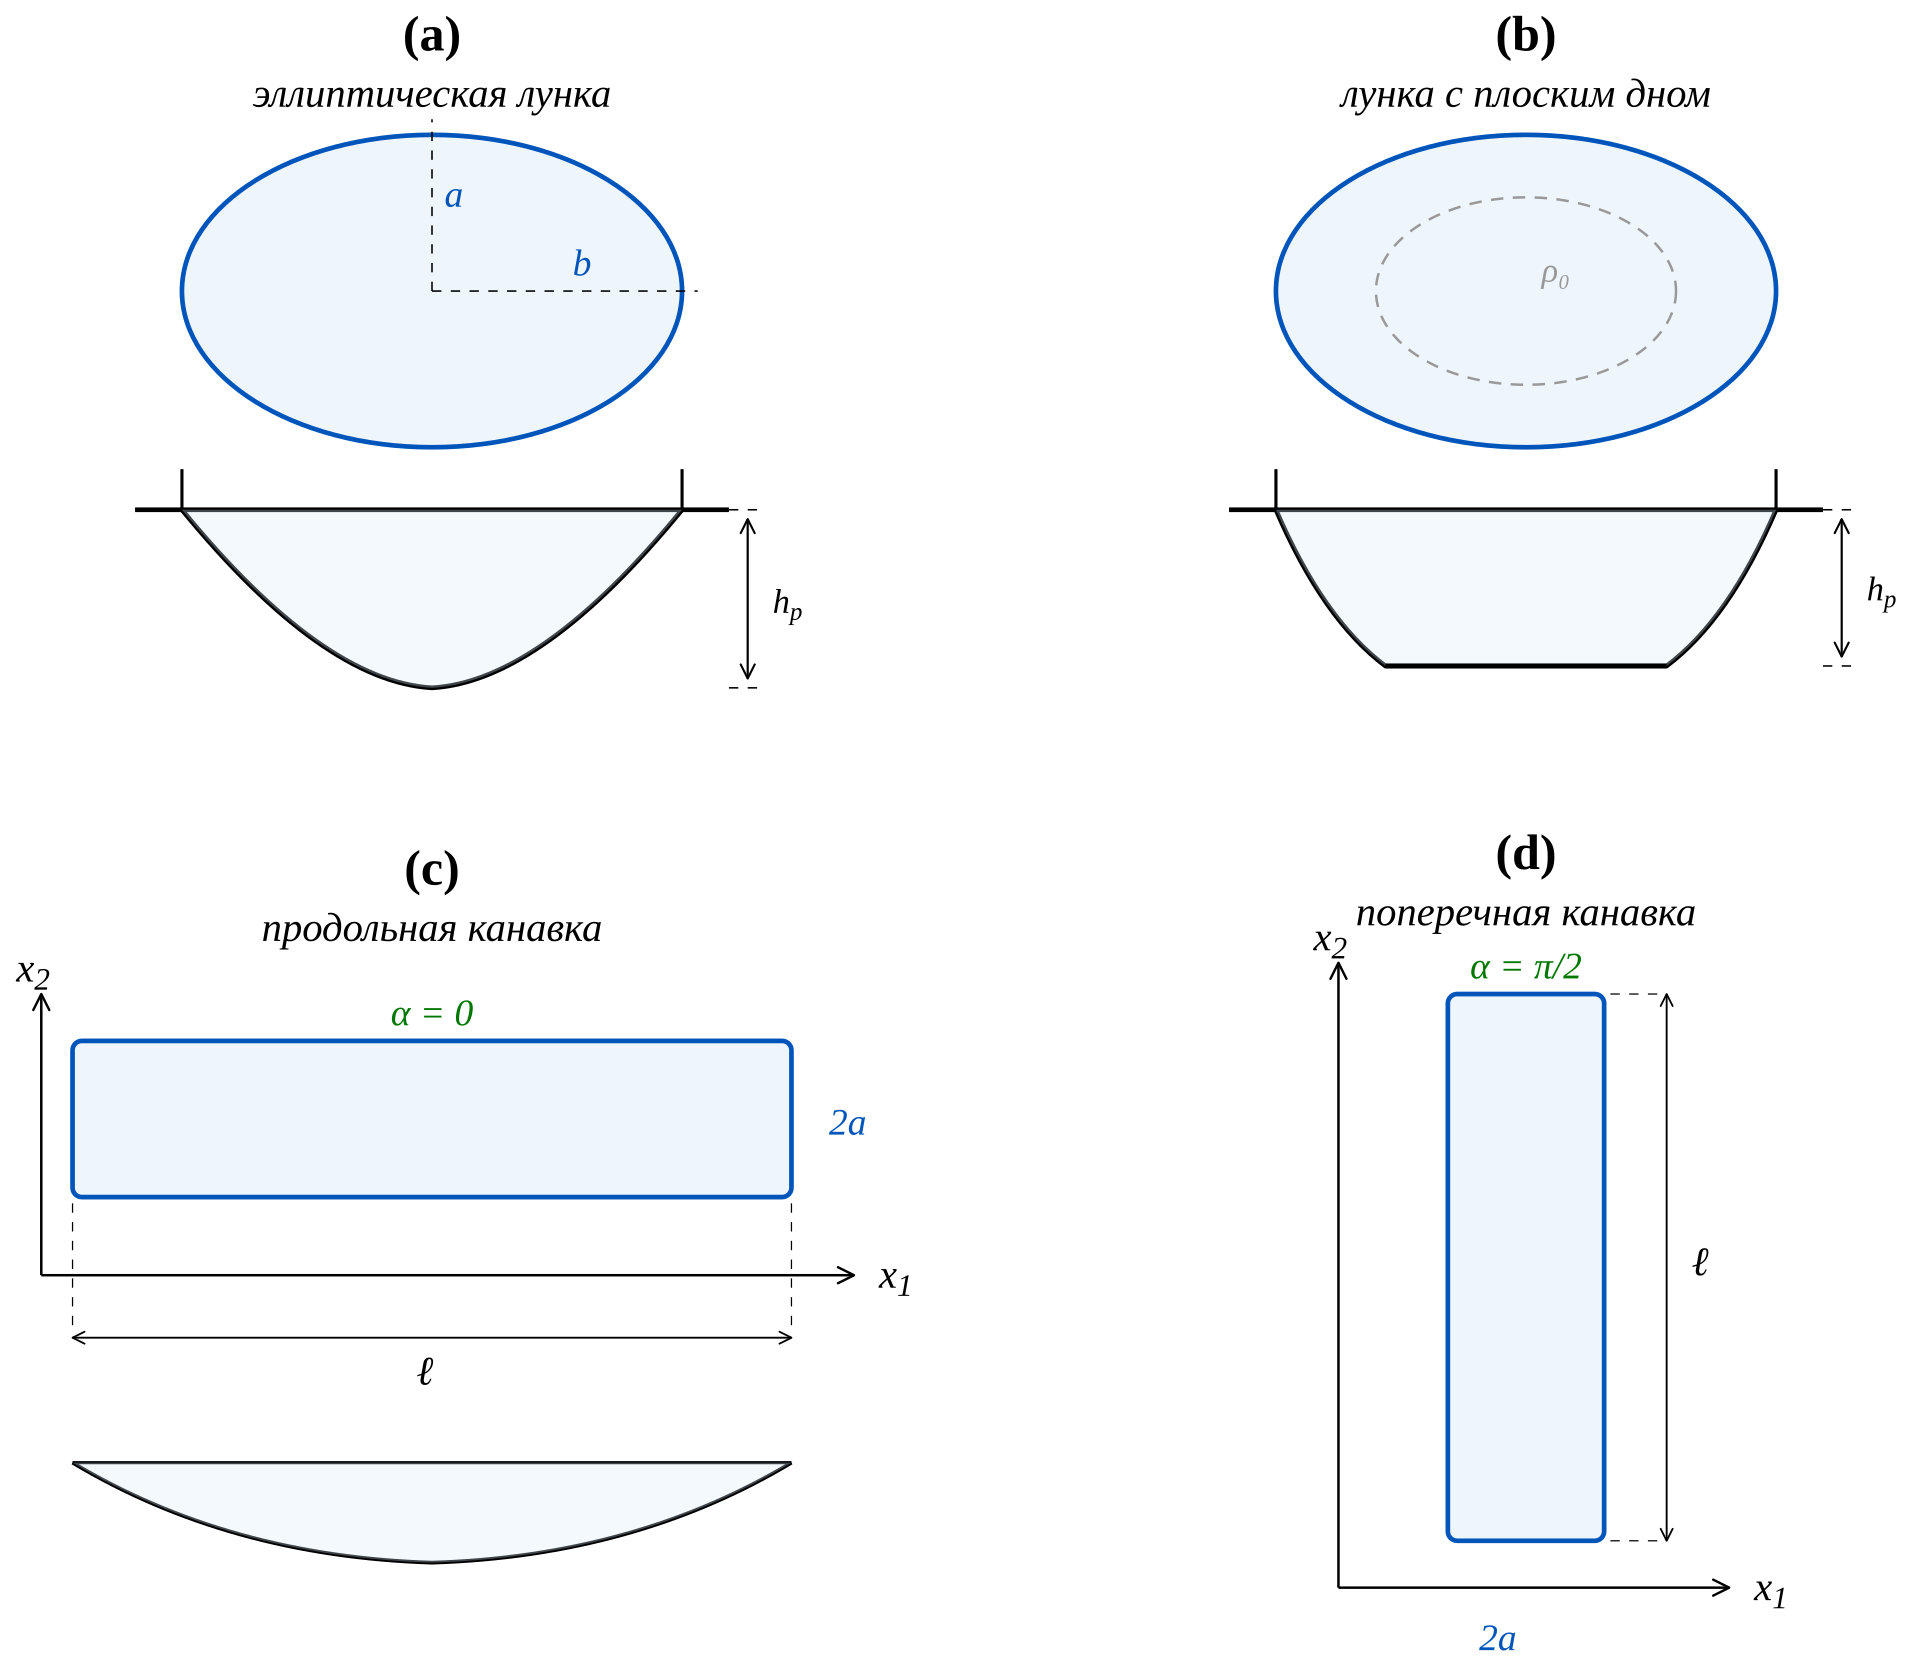
\includegraphics[width=\textwidth,height=0.9\textheight,keepaspectratio]{figures/ch02/fig_2_15.png}
\caption{Основные типы элементов микрорельефа}
\label{fig:texture_geometries}
\end{figure}

%% ===== Завершающий абзац =====

Приведённый набор профильных функций охватывает основные типы
элементов, используемых в практике текстурирования подшипников
скольжения. Выбор конкретного профиля определяется технологией
изготовления и требованиями к гладкости численного решения~\cite{senatore2018,qiangli2019,yujun2023,gropper2018}.
Пространственное расположение элементов на поверхности
рассматривается в подразделе~2.2.3.

\FloatBarrier
\subsection{Варианты расположения микроструктур}

Геометрия отдельного элемента микрорельефа задана
в подразделе~2.2.2. Настоящий подраздел определяет способы
расположения элементов на рабочей поверхности. Результат --
множество центров $\{(x_{1,k},\, x_{2,k})\}_{k=1}^{N}$ (и при
необходимости углов поворота~$\alpha_k$ для канавок). Раскладка
задаётся на прямоугольной области текстурирования
$\Omega_{\mathrm{tex}}
  = [x_{1,s},\, x_{1,t}] \times [x_{2,s},\, x_{2,t}]$
в поверхностных координатах~$(x_1, x_2)$. По периодическому
направлению (например, $x_1 = R\theta$ с периодом $L_1 = 2\pi R$)
координаты центров вычисляются с учётом периодичности по~$x_1$.

%% ===== Блок 1: Прямоугольная решётка =====

\subsubsection*{Прямоугольная решётка}

Базовый тип раскладки. Центры расположены в узлах прямоугольной
сетки с шагами~$p_1$, $p_2$ и начальными смещениями~$\delta_1$,
$\delta_2$:
\begin{equation}
  x_{1,i} = x_{1,s} + \delta_1 + i\,p_1, \quad
  x_{2,j} = x_{2,s} + \delta_2 + j\,p_2,
  \label{eq:layout_rect}
\end{equation}
где $i = 0, 1, \ldots, I_{\max}$; $j = 0, 1, \ldots, J_{\max}$.
Обычно выбирают $0 \leq \delta_1 < p_1$,
$0 \leq \delta_2 < p_2$. Тогда
\[
  I_{\max}
    = \left\lfloor \frac{x_{1,t} - x_{1,s} - \delta_1}{p_1} \right\rfloor,
  \quad
  J_{\max}
    = \left\lfloor \frac{x_{2,t} - x_{2,s} - \delta_2}{p_2} \right\rfloor.
\]

Площадь элементарной ячейки:
$S_{\mathrm{cell}} = p_1 \cdot p_2$.
Коэффициент заполнения (связь с формулой~\eqref{eq:fill_fraction}
из подраздела~2.2.1):
\begin{equation}
  \phi \approx \frac{A_{\mathrm{elem}}}{p_1\,p_2}.
  \label{eq:fill_rect}
\end{equation}

%% ===== Блок 2: Шахматная решётка =====

\subsubsection*{Шахматная решётка}

Чётные и нечётные ряды сдвинуты друг относительно друга на
половину шага по~$x_1$:
\begin{equation}
  \begin{alignedat}{2}
    & x_{2,j}   &\;=\;& x_{2,s} + \delta_2 + j\,p_2, \\
    & x_{1,i,j} &\;=\;& x_{1,s} + \delta_1 + i\,p_1
                  + \tfrac{1}{2}\,p_1\,(j \bmod 2).
  \end{alignedat}
  \label{eq:layout_staggered}
\end{equation}

Индекс~$i$ для фиксированного~$j$ выбирается так, чтобы
$x_{1,i,j} \in [x_{1,s},\, x_{1,t}]$.
Шахматная раскладка повышает равномерность покрытия при тех же
шагах~$p_1$, $p_2$. Площадь элементарной ячейки та же:
$S_{\mathrm{cell}} = p_1 \cdot p_2$.

%% ===== Блок 3: Гексагональная решётка =====

\subsubsection*{Гексагональная решётка}

Является частным случаем шахматной раскладки с определённым
соотношением шагов. Задаётся одним параметром -- расстоянием между
ближайшими центрами~$p$:
\begin{equation}
  p_1 = p, \quad p_2 = \frac{\sqrt{3}}{2}\,p.
  \label{eq:layout_hex}
\end{equation}

Формулы координат -- как для шахматной
решётки~\eqref{eq:layout_staggered} с этими шагами.
Гексагональная раскладка обеспечивает наиболее плотную упаковку
круговых элементов ($a = b$) на плоскости. Площадь элементарной ячейки:
$S_{\mathrm{cell}} = p_1\,p_2 = \frac{\sqrt{3}}{2}\,p^2$.
Соответствующая оценка коэффициента заполнения:
\[
  \phi \approx \frac{A_{\mathrm{elem}}}{S_{\mathrm{cell}}}
    = \frac{2\,A_{\mathrm{elem}}}{\sqrt{3}\,p^2}.
\]

%% ===== Блок 4: Филлотаксис =====

\subsubsection*{Спиральная раскладка (филлотаксис)}

Центры элементов располагаются по спирали Ферма с шагом по углу,
равным золотому углу $\gamma = 2\pi(2 - \varphi)$, где
$\varphi = (1 + \sqrt{5})/2$ -- золотое сечение:
\begin{equation}
  \begin{aligned}
    r_k      &= c\,\sqrt{k}, \\
    \theta_k &= k\,\gamma,
  \end{aligned}
  \quad k = 1, 2, \ldots, N,
  \label{eq:layout_phyllotaxis}
\end{equation}
где $c$ -- масштабный коэффициент, определяющий расстояние между
витками (связан с требуемой плотностью заполнения). Площадь,
приходящаяся на один элемент, приближённо равна $\pi c^2$, откуда
\begin{equation}
  c \approx \sqrt{\frac{A_{\mathrm{tex}}}{\pi\,N}}.
  \label{eq:phyllotaxis_c}
\end{equation}

Координаты
центров в поверхностных координатах $(x_{1,k},\, x_{2,k})$
пересчитываются из $(r_k, \theta_k)$ в зависимости от постановки.

Филлотаксис обеспечивает равномерное заполнение круговой или
кольцевой области без выраженных рядов и столбцов. Раскладка
особенно удобна для кольцевых областей (упорный подшипник).

%% ===== Блок 5: Раскладка канавок =====

\subsubsection*{Раскладка канавок}

Для канавок раскладка упрощается: центры располагаются вдоль одного
направления с постоянным шагом. Например, для канавок,
ориентированных вдоль~$x_1$ ($\alpha_k = 0$), центры задаются как
\[
  x_{2,k} = x_{2,s} + \delta_2 + k\,p_2,
  \quad k = 0, 1, \ldots, N_g - 1,
\]
а $x_{1,k} = (x_{1,s} + x_{1,t})/2$. Для сквозных канавок по всему
периодическому направлению длина $\ell = L_1$.
Для перекрёстных канавок (например, продольные + поперечные)
задаются два семейства с разными углами~$\alpha$.

Основные типы регулярных раскладок показаны на рис.~\ref{fig:layout_staggered}; спиральная раскладка по принципу филлотаксиса -- на рис.~\ref{fig:layout_phyllotaxis}.

%% ===== Блок 6: Рисунки =====

% [РИСУНОК: Типы решёток]
\begin{figure}[!ht]
\centering
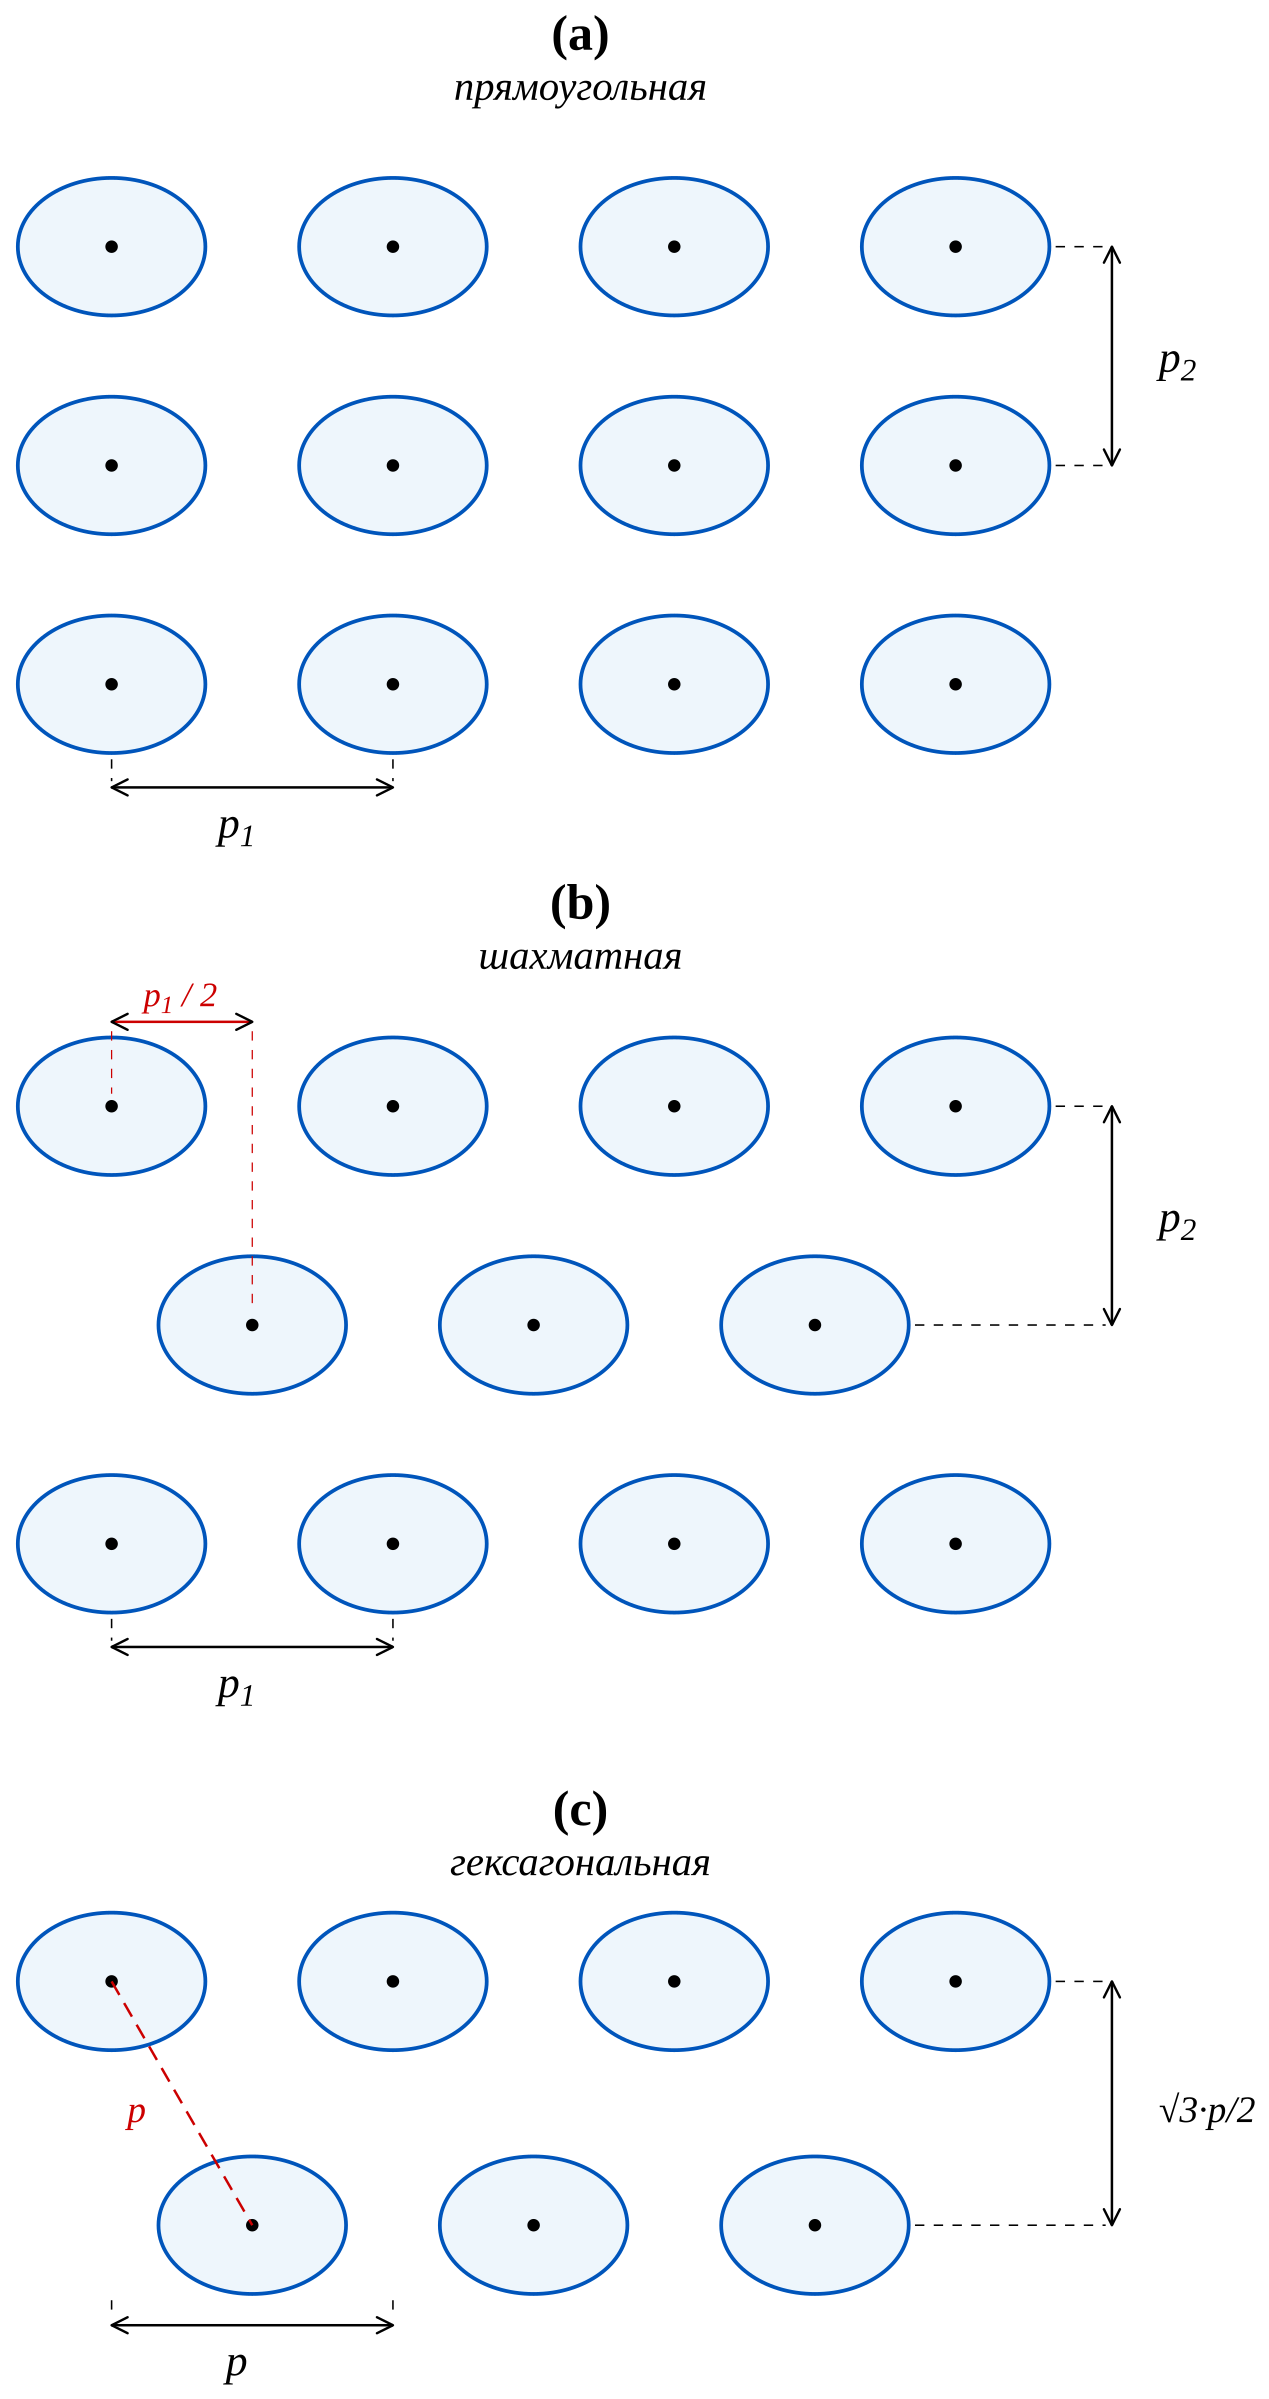
\includegraphics[width=\textwidth,height=0.9\textheight,keepaspectratio]{figures/ch02/fig_2_16.png}
\caption{Основные типы регулярных раскладок микроструктур}
\label{fig:layout_staggered}
\end{figure}

% [РИСУНОК: Филлотаксис]
\begin{figure}[!ht]
\centering
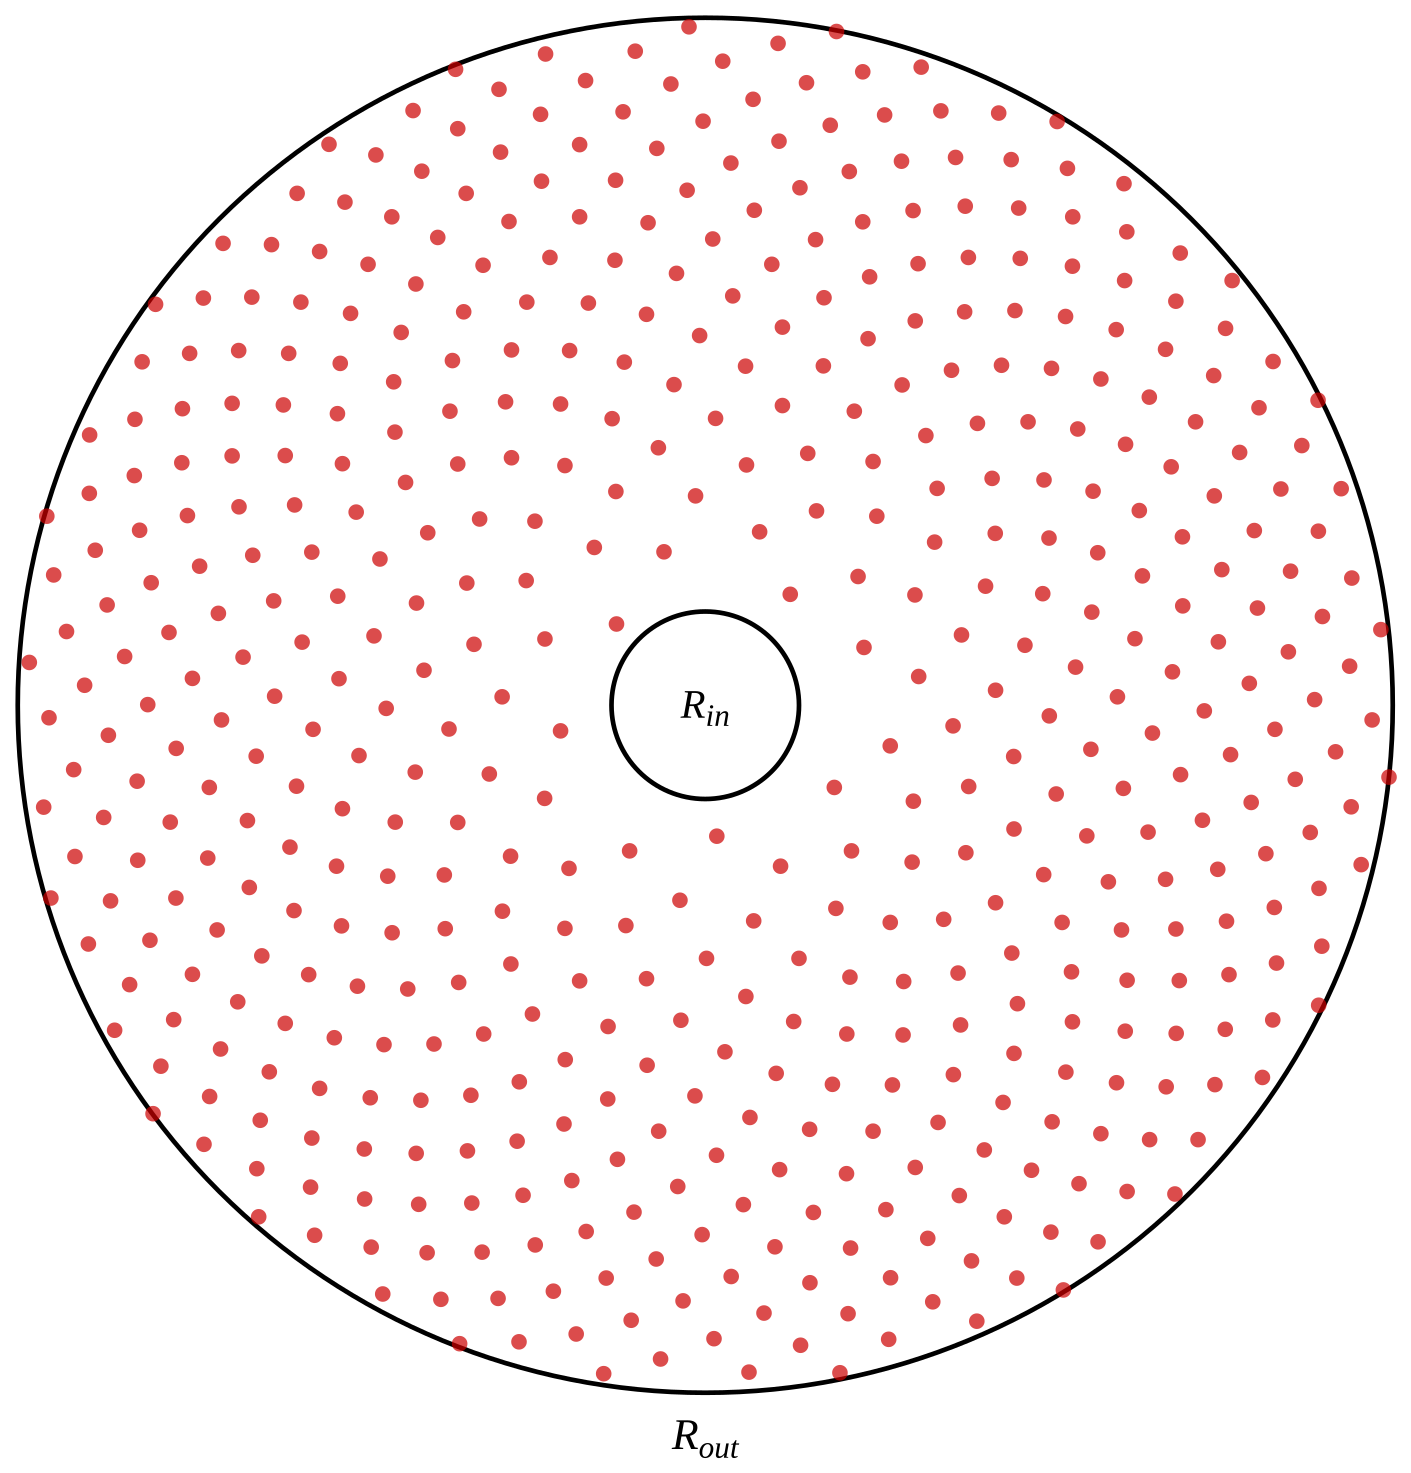
\includegraphics[width=\textwidth,height=0.9\textheight,keepaspectratio]{figures/ch02/fig_2_17.png}
\caption{Раскладка микроструктур по принципу филлотаксиса}
\label{fig:layout_phyllotaxis}
\end{figure}

%% ===== Правило включения центров =====

В настоящей работе элемент считается принадлежащим области
текстурирования, если его центр $(x_{1,k},\, x_{2,k})$ лежит
в~$\Omega_{\mathrm{tex}}$. При необходимости исключения элементов,
частично выходящих за границу, дополнительно требуют, чтобы
область~$D_k$ целиком помещалась в~$\Omega_{\mathrm{tex}}$, что
эквивалентно введению защитных отступов порядка~$a_k$, $b_k$ от границ
области (для однородной текстуры -- $a$, $b$).

%% ===== Завершающий абзац =====

Выбор типа раскладки определяется формой области текстурирования,
типом подшипника и целями параметрического анализа~\cite{senatore2018}. Безразмерные
параметры, характеризующие микрорельеф в целом, вводятся
в подразделе~2.2.4.

\FloatBarrier
\subsection{Безразмерные параметры микрорельефа}

Для параметрического анализа удобно перейти к безразмерным параметрам текстуры.
Используются масштабы, введённые в подразделе~2.1.6
(таблица~\ref{tab:nondim_scales}): характерная толщина зазора~$h_0$
и характерные длины~$L_1$,~$L_2$ по поверхностным координатам~$x_1$,~$x_2$.
Безразмерные координаты и уравнение Рейнольдса уже заданы
в подразделе~2.1.6; здесь нормируются только параметры текстуры.

Ключевым безразмерным параметром является отношение глубины элемента
к характерной толщине зазора:
\begin{equation}\label{eq:Hp_nondim}
  H_p = \frac{h_p}{h_0}.
\end{equation}

Требование применимости уравнения Рейнольдса к текстурированной
поверхности (подраздел~2.1.5) формулируется как $H_p \ll 1$.

Безразмерные полуоси элемента определяются делением на соответствующие
масштабы длины:
\begin{equation}\label{eq:AB_nondim}
  A^{*} = \frac{a}{L_2}, \quad B^{*} = \frac{b}{L_1},
\end{equation}
аспектное отношение элемента:
\begin{equation}\label{eq:kappa}
  \kappa = \frac{a}{b}.
\end{equation}

При $\kappa = 1$ элемент осесимметричен (круговая лунка);
при $\kappa \neq 1$ -- эллиптический.
Заметим, что при $L_1 \neq L_2$ выполняется
\[
  \kappa = \frac{a}{b}
         = \frac{A^{*}}{B^{*}}\,\frac{L_2}{L_1},
\]
а при $L_1 = L_2$ получаем $\kappa = A^{*}/B^{*}$.

Безразмерные шаги раскладки:
\begin{equation}\label{eq:P_nondim}
  P_1^{*} = \frac{p_1}{L_1}, \quad P_2^{*} = \frac{p_2}{L_2}.
\end{equation}

Условия непересечения элементов (подраздел~2.2.1) удобно проверять
через отношения $p_1/(2b)$ и $p_2/(2a)$, которые показывают,
во сколько раз шаг превышает полный размер элемента
($2b$ по $x_1$ и $2a$ по $x_2$).

Коэффициент заполнения~$\phi$ (подраздел~2.2.1) является безразмерным.
Для эллиптических элементов на регулярной решётке при непересекающихся
элементах и пренебрежении краевыми эффектами
\begin{equation}\label{eq:phi_nondim}
  \phi \approx \frac{\pi\, a\, b}{p_1\, p_2}
       = \frac{\pi\, A^{*}\, B^{*}}{P_1^{*}\, P_2^{*}}.
\end{equation}

Полный перечень безразмерных параметров микрорельефа сведён в табл.~\ref{tab:nondim_texture}.

Ряд параметров текстуры является безразмерным по определению:
$\rho_0 \in (0,\,1)$ -- параметр плоского дна (подраздел~2.2.2);
$\alpha$ -- угол ориентации элемента.
Для канавок вводится безразмерная длина $\ell^{*} = \ell / L_1$;
для сквозных канавок по периодическому направлению при выборе
$L_1$ равным длине периода $\ell^{*} = 1$.
Для повёрнутых элементов ($\alpha \neq 0$) используются локальные
координаты из подраздела~2.2.2; переход к безразмерным величинам
выполняется делением длин на соответствующие масштабы из~2.1.6.

\begin{table}[!ht]
\centering
\caption{Безразмерные параметры микрорельефа}
\label{tab:nondim_texture}
\begin{tabularx}{\textwidth}{|X|c|c|}
\hline
\multicolumn{1}{|c|}{\textbf{Параметр}} & \textbf{Обозначение} & \textbf{Определение} \\
\hline
Безразмерная глубина             & $H_p$    & $h_p / h_0$                          \\
\hline
Безразмерная полуось по $x_2$    & $A^{*}$  & $a / L_2$                            \\
\hline
Безразмерная полуось по $x_1$    & $B^{*}$  & $b / L_1$                            \\
\hline
Отношение полуосей               & $\kappa$ & $a / b$                              \\
\hline
Безразмерный шаг по $x_1$        & $P_1^{*}$ & $p_1 / L_1$                        \\
\hline
Безразмерный шаг по $x_2$        & $P_2^{*}$ & $p_2 / L_2$                        \\
\hline
Коэффициент заполнения           & $\phi$   & $N A_{\mathrm{elem}} / A_{\mathrm{tex}}$ \\
\hline
Параметр плоского дна            & $\rho_0$ & $(0,\,1)$                            \\
\hline
Угол ориентации                  & $\alpha$ & --                                   \\
\hline
Безразмерная длина канавки       & $\ell^{*}$ & $\ell / L_1$                       \\
\hline
\end{tabularx}
\end{table}

\FloatBarrier

Введённый набор безразмерных параметров
($H_p$, $A^{*}$, $B^{*}$, $\kappa$, $P_1^{*}$, $P_2^{*}$, $\phi$, $\rho_0$, $\ell^{*}$)
позволяет проводить параметрические исследования и сравнивать результаты
для различных типов подшипников при одинаковых безразмерных группах.

Физический смысл каждого безразмерного параметра элемента
микрорельефа целесообразно кратко прокомментировать.
Глубина~$H_p = h_p/h_0$ задаёт масштаб добавки к зазору
относительно характерной толщины плёнки. При $H_p \ll 1$
лунка неглубокая; её гидродинамический эффект мал, так как
создаваемый ею дополнительный клин пропорционален $H_p$.
При $H_p \gtrsim 1$ глубина лунки сопоставима с зазором,
что может нарушить течение в соседних ячейках и снизить
несущую способность; для эллипсоидальных лунок оптимальная
глубина, как правило, находится в диапазоне
$H_p \approx 0{,}2$--$0{,}5$.

Безразмерные полуоси~$A^{*}$, $B^{*}$ задают размеры элемента
относительно длин расчётной области в каждом из координатных
направлений. Произведение~$\pi A^{*} B^{*}$ пропорционально
безразмерной площади одной лунки; коэффициент
покрытия~$\phi$ определяет суммарную долю текстурированной
площади. Ориентация эллипса ($A^{*} \neq B^{*}$) влияет
на анизотропию гидродинамического эффекта и, следовательно,
на соотношение между несущей способностью, трением и утечками.

Шаги~$P_1^{*}$, $P_2^{*}$ (периоды раскладки по~$s_1$
и~$s_2$ соответственно) совместно с~$A^{*}$, $B^{*}$
и~$\phi$ образуют замкнутый набор параметров текстуры,
достаточный для однозначного задания шахматной раскладки.
При шахматной схеме реальный шаг в нечётных рядах сдвигается
на $P_1^{*}/2$, что обеспечивает более равномерное перекрытие
поверхности при той же плотности.

\textit{Конкуренция двух гидродинамических эффектов.}
Влияние микроструктур на~несущую способность определяется конкуренцией двух противоположно направленных механизмов. Первый механизм~--- генерация давления: передняя стенка лунки создаёт дополнительный сходящийся клин, что усиливает гидродинамический эффект и~повышает давление над~лункой. Второй механизм~--- сброс давления: задняя стенка лунки образует расходящийся клин, где давление падает; при~глубоких лунках в~этой зоне формируется локальная кавитационная область, которая обрывает возможность дальнейшего нарастания давления. Суммарный эффект на~несущую способность определяется соотношением этих двух вкладов.

При~малых глубинах~$H_p \ll 1$ первый механизм преобладает, и~несущая способность монотонно возрастает с~ростом~$H_p$. При~чрезмерно глубоких лунках~$H_p \gtrsim 1$ кавитационная зона занимает значительную часть задней стенки, суммарный вклад становится отрицательным, и~несущая способность начинает снижаться относительно гладкой поверхности. Следствием является существование оптимальной глубины~$H_p^{*}$, при~которой несущая способность максимальна. Для~эллипсоидальных лунок в~типичных конфигурациях этот оптимум находится в~диапазоне $H_p^{*} \approx 0{,}2$--$0{,}5$~--- именно эти значения использованы в~главах~5--7.

Аналогичная конкуренция наблюдается по~параметру коэффициента покрытия~$\phi$. При~малых~$\phi$ лунки редки и~суммарный гидродинамический эффект мал; при~$\phi \to 1$ лунки занимают практически всю поверхность, клиновой эффект между лунками исчезает и~несущая способность снова снижается. Оптимальный коэффициент покрытия для~радиальных и~упорных подшипников, по~данным численных и~экспериментальных исследований, как~правило, находится в~диапазоне $\phi \approx 0{,}1$--$0{,}4$, хотя точное значение зависит от~типа подшипника, режима нагружения и~формы элементов микрорельефа.

\textit{Конкуренция двух гидродинамических эффектов.}
Влияние микроструктур на~несущую способность определяется конкуренцией двух противоположно направленных механизмов. Первый механизм --- генерация давления: передняя стенка лунки создаёт дополнительный сходящийся клин, что усиливает гидродинамический эффект и~повышает давление над~лункой. Второй механизм --- сброс давления: задняя стенка лунки образует расходящийся клин, где давление падает; при~глубоких лунках в~этой зоне формируется локальная кавитационная область, которая обрывает возможность дальнейшего нарастания давления. Суммарный эффект на~несущую способность определяется соотношением этих двух вкладов.

При~малых глубинах~$H_p \ll 1$ первый механизм преобладает, и~несущая способность монотонно возрастает с~ростом~$H_p$. При~чрезмерно глубоких лунках~$H_p \gtrsim 1$ кавитационная зона занимает значительную часть задней стенки, суммарный вклад становится отрицательным, и~несущая способность начинает снижаться относительно гладкой поверхности. Следствием является существование оптимальной глубины~$H_p^{*}$, при~которой несущая способность максимальна. Для~эллипсоидальных лунок в~типичных конфигурациях этот оптимум находится в~диапазоне $H_p^{*} \approx 0{,}2$--$0{,}5$~--- именно эти значения использованы в~главах~5--7.

Аналогичная конкуренция наблюдается по~параметру коэффициента покрытия~$\phi$. При~малых~$\phi$ лунки редки и~суммарный гидродинамический эффект мал; при~$\phi \to 1$ лунки занимают практически всю поверхность, клиновой эффект между лунками исчезает и~несущая способность снова снижается. Оптимальный коэффициент покрытия для~радиальных и~упорных подшипников, по~данным численных и~экспериментальных исследований, находится в~диапазоне $\phi \approx 0{,}1$--$0{,}4$, хотя точное значение зависит от~типа подшипника, режима нагружения и~формы элементов микрорельефа~\cite{senatore2018}.


\FloatBarrier
\section{Кавитация и уравнения JFO (массо-сохраняющая постановка)}
\subsection{Физика разрыва плёнки и ограничения модели с обнулением давления}

%% Блок 1: Постановка проблемы — откуда p < 0
Уравнение Рейнольдса для полностью заполненного зазора
(подразделы~2.1.2-2.1.4) в ряде случаев даёт области
с~$p < 0$ -- как правило, в зоне расходящегося клина, за максимумом
давления.  Математически это следствие граничных условий и допущения
сплошного заполнения зазора жидкостью.  Физически отрицательное
давление означает, что жидкость находится в состоянии растяжения,
что для смазочных жидкостей допустимо лишь в узком диапазоне.
Отрицательное давление в классическом решении -- индикатор того,
что допущение полного заполнения зазора жидкостью перестаёт быть
корректным.

%% Блок 2: Физическая картина — разрыв плёнки и кавитация
При снижении давления ниже некоторого порога~$p_{\mathrm{cav}}$ (кавитационного давления, обычно близкого к давлению насыщенных паров или окружающей среды)
происходит выделение растворённого газа из смазочной жидкости,
образование парогазовых полостей (каверн) и формирование двухфазной
области (жидкость~+ газ/пар), в которой давление приблизительно
постоянно и равно~$p_{\mathrm{cav}}$.  В результате расчётная область
разделяется на характерные зоны (рис.~\ref{fig:cavitation_scheme}): зона полного заполнения
($p > p_{\mathrm{cav}}$), зона кавитации (частичное заполнение,
$p \approx p_{\mathrm{cav}}$), граница разрыва (переход от полного
заполнения к кавитации) и граница восстановления (реформация --
обратный переход).  Между границами разрыва и восстановления зазор
заполнен смесью жидкости и газа, причём объёмная доля жидкости
убывает по мере удаления от границы разрыва.  В инженерной модели
обычно принимают~$p_{\mathrm{cav}}$ постоянным; при работе
с избыточными давлениями часто полагают $p_{\mathrm{cav}} = 0$.

%% Блок 7: Рисунок (после физической картины, до обнуления давления)
\begin{figure}[!ht]
\centering
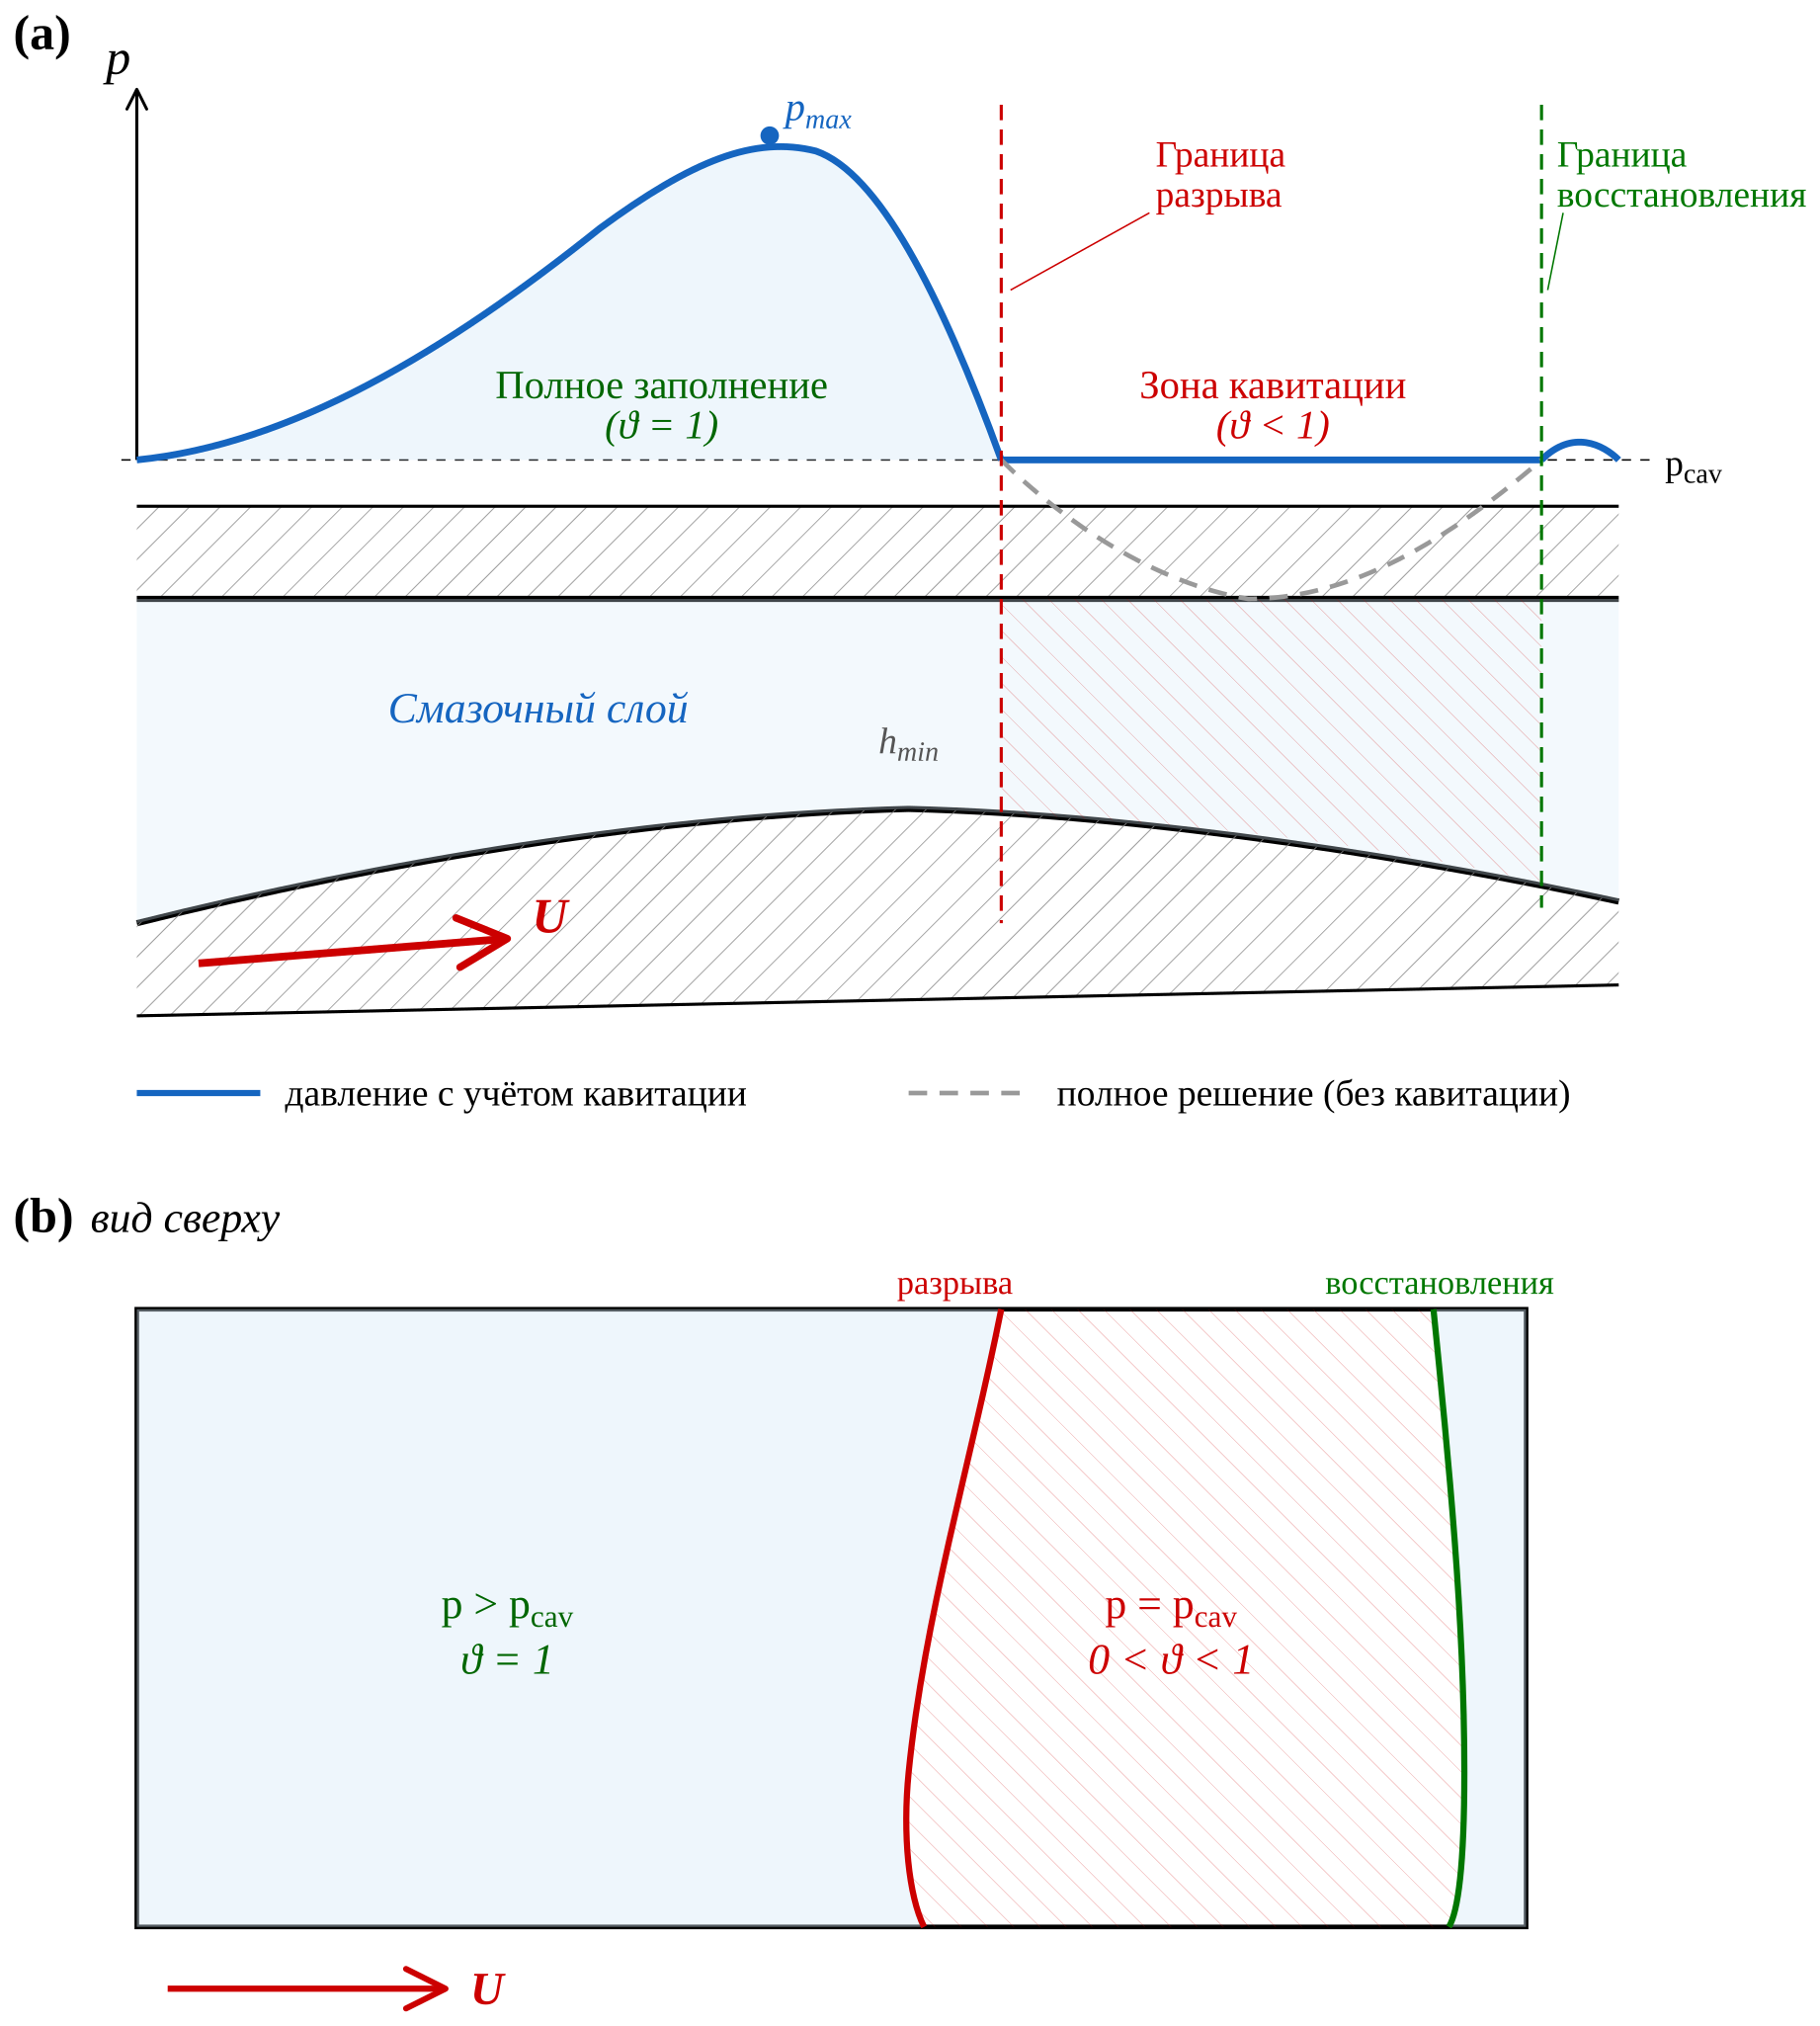
\includegraphics[width=\textwidth,height=0.9\textheight,keepaspectratio]{figures/ch02/fig_2_18.png}
\caption{Схема кавитации в смазочном слое: продольный разрез~(a)
  и вид сверху~(b)}
\label{fig:cavitation_scheme}
\end{figure}

%% Блок 3: Простой приём — обнуление давления
Наиболее распространённый инженерный подход к устранению нефизичных
отрицательных давлений состоит в замене~$p$ на~$p_{\mathrm{cav}}$
в областях, где решение даёт $p < p_{\mathrm{cav}}$.
Этот приём (условие Гюмбеля, half-Sommerfeld) позволяет получить
приемлемые оценки несущей способности и формы поля давления.
Однако он является неполной физической моделью, поскольку
кавитация -- не просто $p = p_{\mathrm{cav}}$, а ещё и частичное
заполнение зазора.

%% Блок 4: Главный недостаток — нарушение баланса массы
Уравнение Рейнольдса выведено из уравнения неразрывности при
допущении полного заполнения зазора ($\vartheta = 1$, где $\vartheta$ --
степень заполнения).  Типовой удельный расход (объёмный поток) в плёнке имеет вид
\begin{equation}\label{eq:q_film}
  \mathbf{q} = -\frac{h^3}{12\mu}\,\nabla p
    + \frac{h}{2}\,\mathbf{U},
\end{equation}
где $\mathbf{U}$ -- скорость относительного скольжения поверхностей.
Для полностью заполненного зазора ($\vartheta = 1$) выполняется
уравнение неразрывности:
\begin{equation}\label{eq:continuity_film}
  \frac{\partial h}{\partial t} + \nabla \cdot \mathbf{q} = 0.
\end{equation}

Если «отрезать» отрицательные давления, то меняется градиент
давления~$\nabla p$ и, следовательно, поток~$\mathbf{q}$, но при этом
не вводится переменная, описывающая частичное заполнение.  В результате
на границах кавитационной зоны возникают нефизичные источники или стоки
массы.  Эффект особенно заметен при расчётах расхода смазки
и в нестационарных задачах (подвижные микроструктуры, переходные
режимы).  Таким образом, корректная модель должна одновременно
описывать (а)~давление и (б)~степень заполнения в кавитационной
области.

%% Блок 5: Требования к корректной модели кавитации
Сформулируем минимальные требования к модели кавитации:
\begin{enumerate}
  \item $p \geq p_{\mathrm{cav}}$ во всей расчётной области.
  \item В зоне полного заполнения ($\vartheta = 1$) действует
        классическое уравнение Рейнольдса.
  \item В кавитационной зоне ($\vartheta < 1$) давление фиксировано
        $p = p_{\mathrm{cav}}$, а состояние смеси описывается
        дополнительной переменной $\vartheta \in (0,\, 1]$.
  \item Сохранение массы через границу зон (непрерывность нормальной компоненты потока).
\end{enumerate}

%% Блок 5b: Алгоритм Элрода
Первый практический численный алгоритм решения задачи JFO предложен
Elrod и Adams~\cite{elrod1975}: вводится переключающая функция~$g$
($g=1$ в зоне полного заполнения, $g=0$ в зоне кавитации),
позволяющая записать единое уравнение для всей расчётной области
без явного отслеживания границ кавитации.
Алгоритм Элрода получил широкое распространение и лёг в основу
большинства последующих реализаций массосохраняющей кавитации.
В настоящей работе используется альтернативный подход на основе
итераций по активному множеству (подраздел~2.3.3),
обеспечивающий аналогичный результат.

%% Блок 6: Подводка к JFO
Перечисленным требованиям удовлетворяет массосохраняющая постановка
Якобссона--Флоберга--Ольссона (JFO), в которой кавитационная зона
описывается не только условием $p = p_{\mathrm{cav}}$, но и переменной
степенью заполнения~$\vartheta$.  Соответствующие уравнения формулируются
в подразделе~2.3.2~\cite{dhande2018}.

\FloatBarrier
\subsection{Массосохраняющая постановка кавитации (JFO)}

%% Блок 1: Вводный абзац
В подразделе~2.3.1 введены кавитационное давление~$p_{\mathrm{cav}}$
и степень заполнения~$\vartheta \in (0,\,1]$.  Цель настоящего раздела --
записать замкнутую систему уравнений для двух искомых переменных:
давления $p(x_1, x_2, t)$ и степени заполнения
$\vartheta(x_1, x_2, t)$, удовлетворяющую требованиям~1-4,
сформулированным в подразделе~2.3.1.  Толщина зазора
$h(x_1, x_2, t)$ считается заданной (суперпозиция из
подраздела~2.2.1).

%% Блок 2: Модифицированное уравнение неразрывности
В кавитационной зоне зазор заполнен жидкостью лишь частично,
поэтому эффективная толщина жидкого слоя равна~$\vartheta\,h$.
Подстановка этой величины в уравнение неразрывности приводит
к модифицированному уравнению Рейнольдса (уравнение JFO):
\begin{equation}\label{eq:jfo_conservation}
  \frac{\partial (\vartheta\,h)}{\partial t}
  + \nabla \cdot \!\left(
    -\,\frac{h^3}{12\mu}\,\nabla p
    + \frac{\vartheta\,h}{2}\,\mathbf{U}
  \right) = 0.
\end{equation}

Первое слагаемое в дивергенции представляет собой пуазейлевский
(напорный) поток, пропорциональный градиенту давления~$\nabla p$.
Второе слагаемое -- куэттовский (переносной) поток, обусловленный
движением поверхности со скоростью~$\mathbf{U}$.  При $\vartheta = 1$
уравнение~\eqref{eq:jfo_conservation} сводится к классическому
уравнению Рейнольдса.  Здесь операторы $\nabla$ и $\nabla\!\cdot$
понимаются в поверхностных координатах, соответствующих выбранной
постановке (подраздел~2.1.6).  Множитель~$\vartheta$ входит в член
накопления и в куэттовский поток.  В кавитационной зоне
$p = p_{\mathrm{cav}}$, поэтому $\nabla p = 0$ и напорный поток
отсутствует автоматически.

Принципиальное отличие постановки JFO от упрощённых моделей кавитации состоит в~следующем. В~модели Гюмбеля отрицательные давления просто обнуляются: $p := \max(p,\, p_{\mathrm{cav}})$ без какого-либо уравнения для кавитационной зоны. Это нарушает баланс масс: куэттовский поток в~зону кавитации не~компенсируется потоком из~неё, и~расход жидкости через замкнутый контур оказывается ненулевым. Следствием является систематическое завышение несущей способности по сравнению с~более точными расчётами, что подтверждается экспериментально: при высоких числах Зоммерфельда отклонение может достигать десятков процентов.

В~постановке JFO вместо простого обнуления давления вводится степень заполнения~$\vartheta$, которая описывает долю объёма зазора, занятую жидкостью. В~зоне полного заполнения $\vartheta = 1$ и~уравнение~\eqref{eq:jfo_conservation} совпадает с~классическим уравнением Рейнольдса. В~кавитационной зоне $p = p_{\mathrm{cav}}$ и~$\vartheta < 1$: жидкость и~газовые пузырьки сосуществуют в~зазоре, причём их~относительные доли изменяются так, чтобы выполнялся баланс масс. Именно введение~$\vartheta$ позволяет разрешить противоречие: давление не~опускается ниже~$p_{\mathrm{cav}}$, а~массовый баланс при~этом сохраняется.

Принципиальное отличие постановки JFO от упрощённых моделей кавитации состоит в~следующем. В~модели Гюмбеля отрицательные давления просто обнуляются: $p := \max(p,\, p_{\mathrm{cav}})$ без какого-либо уравнения для кавитационной зоны. Это нарушает баланс масс: куэттовский поток в~зону кавитации не~компенсируется потоком из~неё, и~расход жидкости через замкнутый контур оказывается ненулевым. Следствием является систематическое завышение несущей способности по сравнению с~более точными расчётами, что подтверждается экспериментально: при высоких числах Зоммерфельда отклонение может достигать десятков процентов.

В~постановке JFO вместо простого обнуления давления вводится степень заполнения~$\vartheta$, которая описывает долю объёма зазора, занятую жидкостью. В~зоне полного заполнения $\vartheta = 1$ и~уравнение~\eqref{eq:jfo_conservation} совпадает с~классическим уравнением Рейнольдса. В~кавитационной зоне $p = p_{\mathrm{cav}}$ и~$\vartheta < 1$: жидкость и~газовые пузырьки сосуществуют в~зазоре, причём их~относительные доли изменяются так, чтобы выполнялся баланс масс. Именно введение~$\vartheta$ позволяет разрешить противоречие: давление не~опускается ниже~$p_{\mathrm{cav}}$, а~массовый баланс при~этом сохраняется.

%% Блок 3: Условия комплементарности
Разделение расчётной области на зону полного заполнения и зону
кавитации определяется условиями комплементарности:
\begin{equation}\label{eq:jfo_complementarity}
  \begin{aligned}
    &p - p_{\mathrm{cav}} \geq 0, \\
    &0 \leq \vartheta \leq 1, \\
    &(p - p_{\mathrm{cav}})\,(1 - \vartheta) = 0.
  \end{aligned}
\end{equation}

Из этих условий следует: либо $p > p_{\mathrm{cav}}$ и тогда
$\vartheta = 1$ (полное заполнение), либо $\vartheta < 1$ и тогда
$p = p_{\mathrm{cav}}$ (кавитация).  Промежуточные состояния
($p > p_{\mathrm{cav}}$ и одновременно $\vartheta < 1$) исключены.
Вместе с уравнением~\eqref{eq:jfo_conservation}
условия~\eqref{eq:jfo_complementarity} образуют замкнутую задачу
для двух неизвестных~$p$ и~$\vartheta$.

Задача~\eqref{eq:jfo_conservation}--\eqref{eq:jfo_complementarity} относится к~классу задач со~свободными границами. Граница разрыва плёнки~-- линия, на~которой $\vartheta$ убывает от~1 до~значения меньше единицы~-- и~граница восстановления плёнки~-- линия, на~которой $\vartheta$ возвращается к~единице~-- не~фиксируются заранее, а~определяются в~ходе решения как часть ответа. Именно эта особенность делает задачу нелинейной даже при линейном уравнении~\eqref{eq:jfo_conservation}: нелинейность сосредоточена в~условиях комплементарности~\eqref{eq:jfo_complementarity}, которые определяют разбиение расчётной области.

Для гладкой поверхности кавитационная зона, как правило, одна и~связна: плёнка разрывается в~расходящемся клине и~восстанавливается на~входе в~следующий период. При~текстурированной поверхности картина принципиально меняется: каждая лунка формирует собственную локальную кавитационную зону в~своей задней части. В~результате расчётная область содержит множество небольших, пространственно разрозненных кавитационных участков. Для~такого решения обеспечение баланса масс становится критически важным: простое обнуление давления приводит к~тому, что каждая лунка <<теряет>> часть массы, и~суммарная ошибка пропорциональна числу лунок~-- она может достигать значимых величин при~высокой плотности текстуры.

Именно поэтому постановка JFO представляет особую ценность при~анализе подшипников с~детерминированными микроструктурами. При~большом числе лунок (порядка~100 и~более на~расчётную область) ошибка, накапливаемая при~использовании упрощённой кавитации, может искажать как~интегральные характеристики (несущую способность, момент трения), так и~пространственное распределение давления. Массосохраняющая постановка лишена этого недостатка по~построению.

Задача~\eqref{eq:jfo_conservation}--\eqref{eq:jfo_complementarity} относится к~классу задач со~свободными границами. Граница разрыва плёнки~-- линия, на~которой $\vartheta$ убывает от~1 до~значения меньше единицы~-- и~граница восстановления плёнки~-- линия, на~которой $\vartheta$ возвращается к~единице~-- не~фиксируются заранее, а~определяются в~ходе решения как часть ответа. Именно эта особенность делает задачу нелинейной даже при линейном уравнении~\eqref{eq:jfo_conservation}: нелинейность сосредоточена в~условиях комплементарности~\eqref{eq:jfo_complementarity}, которые определяют разбиение расчётной области.

Для гладкой поверхности кавитационная зона, как правило, одна и~связна: плёнка разрывается в~расходящемся клине и~восстанавливается на~входе в~следующий период. При~текстурированной поверхности картина принципиально меняется: каждая лунка формирует собственную локальную кавитационную зону в~своей задней части. В~результате расчётная область содержит множество небольших, пространственно разрозненных кавитационных участков. Для~такого решения обеспечение баланса масс становится критически важным: простое обнуление давления приводит к~тому, что каждая лунка <<теряет>> часть массы, и~суммарная ошибка пропорциональна числу лунок~-- она может достигать значимых величин при~высокой плотности текстуры.

Именно поэтому постановка JFO представляет особую ценность при~анализе подшипников с~детерминированными микроструктурами. При~большом числе лунок (порядка~100 и~более на~расчётную область) ошибка, накапливаемая при~использовании упрощённой кавитации, может искажать как~интегральные характеристики (несущую способность, момент трения), так и~пространственное распределение давления. Массосохраняющая постановка лишена этого недостатка по~построению.

%% Рисунок
\begin{figure}[!ht]
\centering
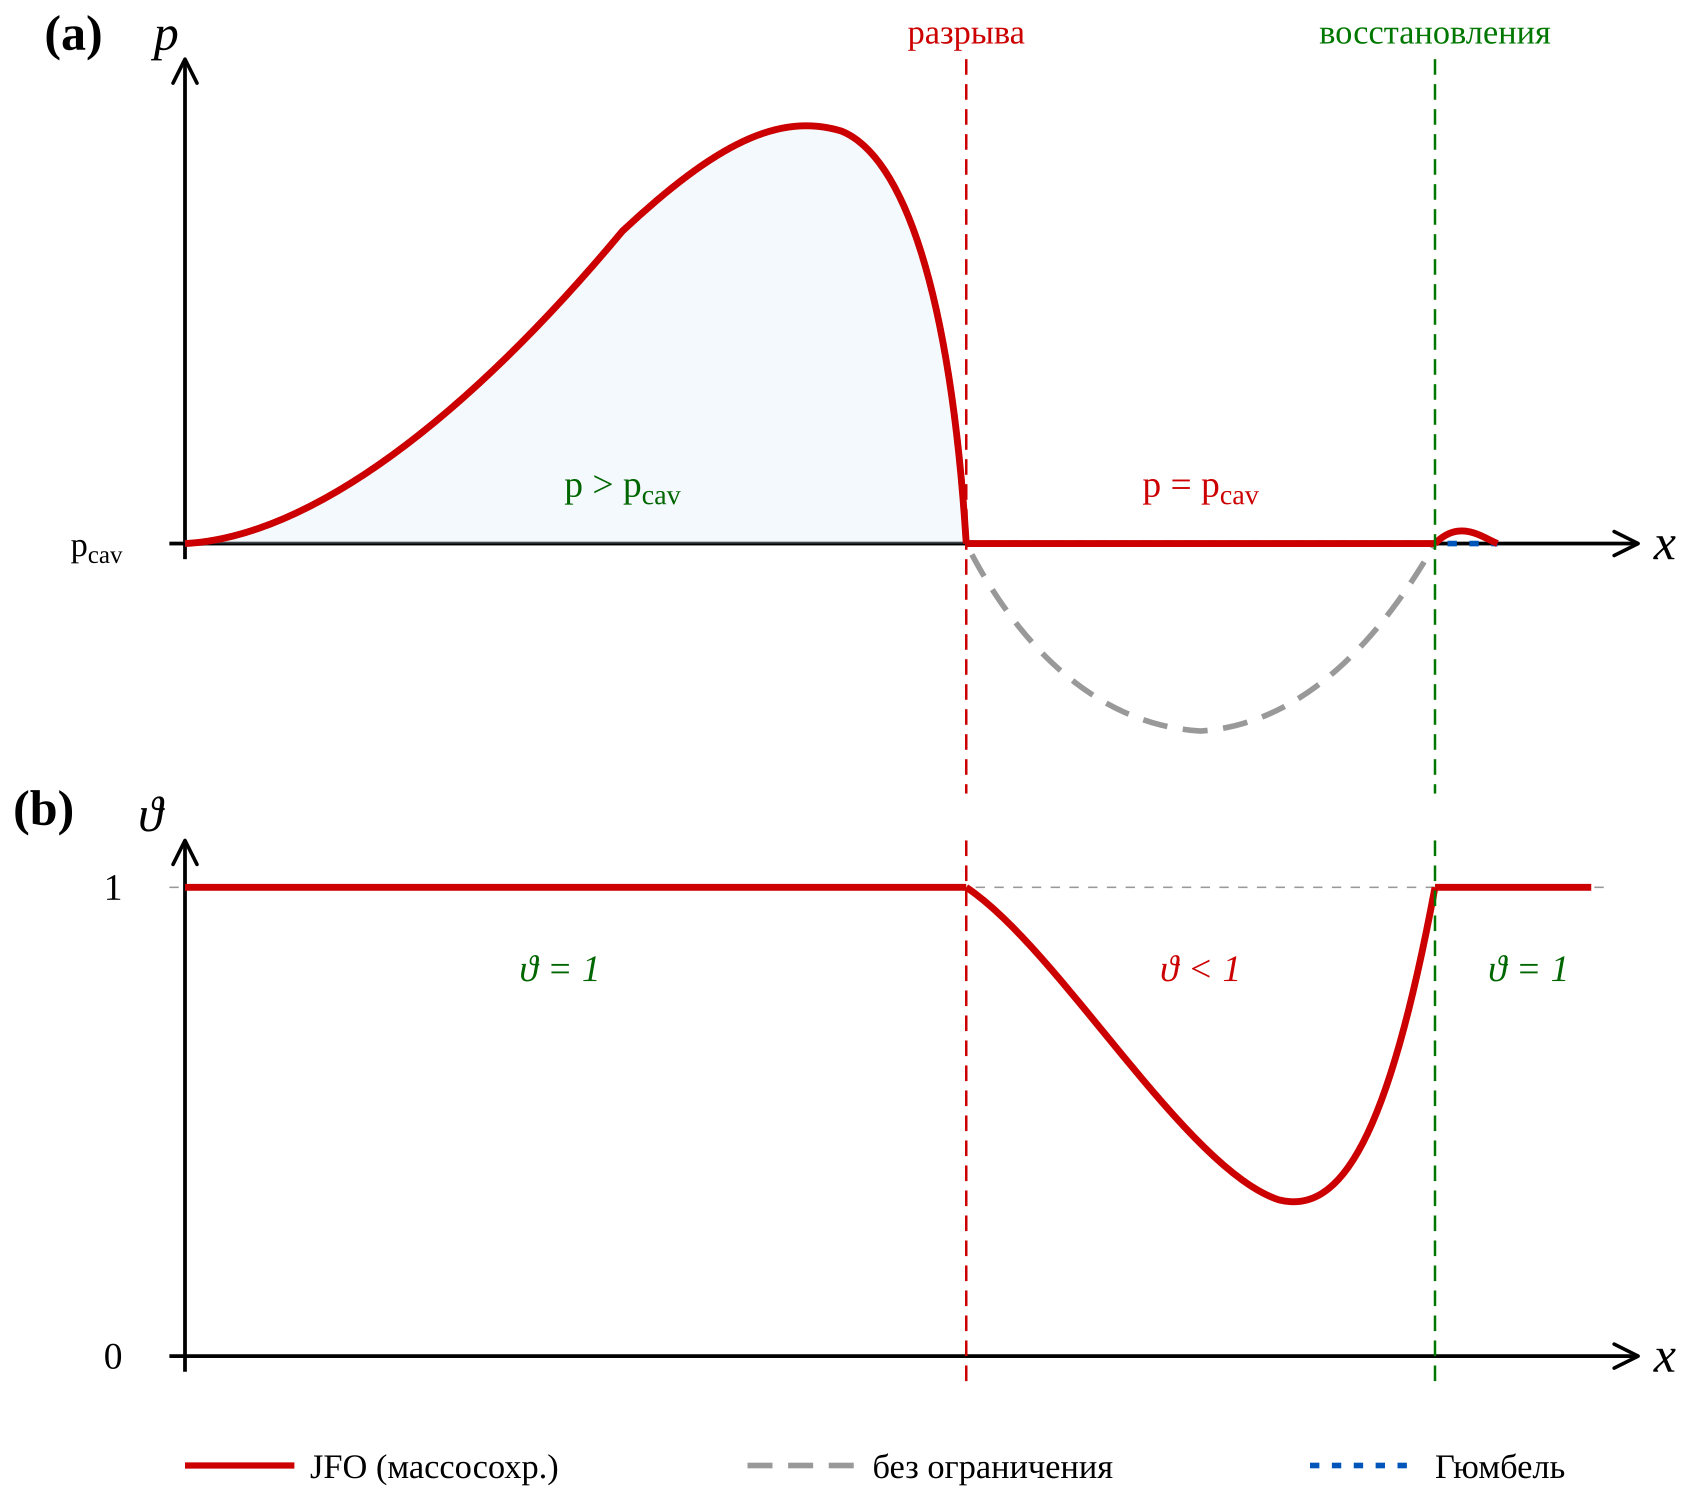
\includegraphics[width=\textwidth,height=0.9\textheight,keepaspectratio]{figures/ch02/fig_2_19.png}
\caption{Сравнение моделей кавитации: обнуление давления (Гюмбель)
  и массосохраняющая постановка (JFO)}
\label{fig:jfo_1d_profile}
\end{figure}

%% Блок 4: Граничные условия
Граничные условия для давления задаются так же, как в
подразделах~2.1.2-2.1.4 (периодичность, заданное давление на входе
и~выходе).  На границах подачи смазки полагают $\vartheta = 1$
(полное заполнение).  По периодическим направлениям~$\vartheta$
подчиняется тем же условиям периодичности, что и~$p$.

%% Блок 5: Подводка к численной реализации
Задача~\eqref{eq:jfo_conservation}-\eqref{eq:jfo_complementarity}
является нелинейной задачей с неравенствами (комплементарность).
На практике её решают итерационно: на каждой итерации определяется
активное множество кавитации и полного заполнения, после чего
обновляются $p$ и $\vartheta$ при выполнении условий комплементарности.
Сравнение моделей кавитации (обнуление давления и JFO) на одномерном профиле давления иллюстрирует рис.~\ref{fig:jfo_1d_profile}. Численная схема дискретизации и алгоритм итерационного решения
приводятся в подразделе~2.3.3~\cite{elrod1975}.

\FloatBarrier
\subsection{Дискретизация уравнений JFO}

%% Блок 1: Вводный абзац
Задача~\eqref{eq:jfo_conservation}-\eqref{eq:jfo_complementarity}
является нелинейной комплементарной задачей: одновременно определяются
давление~$p$ и степень заполнения~$\vartheta$ при выполнении
неравенств.  Решение выполняется итерационно по стратегии активного
множества (active-set): на каждой итерации обновляется разбиение
области на зону полного заполнения и зону кавитации.  В настоящем
подразделе приводится общая схема алгоритма; детали дискретизации,
аппроксимации потоков и выбора солвера описаны в главе~3.

%% Блок 2: Сетка
Расчётная область покрывается равномерной сеткой:
\begin{equation}\label{eq:jfo_grid}
  \begin{aligned}
    &x_{1,i} = x_{1,s} + i\,\Delta x_1, \quad i = 0, \ldots, N_1 - 1, \\
    &x_{2,j} = x_{2,s} + j\,\Delta x_2, \quad j = 0, \ldots, N_2 - 1.
  \end{aligned}
\end{equation}

По периодическим направлениям применяются соответствующие условия
замыкания.  Операторы $\nabla$, $\nabla\!\cdot$ дискретизуются
в поверхностных координатах (подраздел~2.1.6); конкретные разностные
аппроксимации приведены в главе~3.

%% Блок 3: Консервативная дискретизация
Уравнение~\eqref{eq:jfo_conservation} записывается в дискретной
консервативной форме:
\begin{equation}\label{eq:jfo_discrete}
  \frac{(\vartheta h)_{i,j}^{n+1} - (\vartheta h)_{i,j}^{n}}{\Delta t}
  + \frac{F_{i+\frac{1}{2},j} - F_{i-\frac{1}{2},j}}{\Delta x_1}
  + \frac{G_{i,j+\frac{1}{2}} - G_{i,j-\frac{1}{2}}}{\Delta x_2}
  = 0,
\end{equation}
где $F$ и $G$ -- дискретные потоки по направлениям $x_1$ и $x_2$,
соответствующие напорному и переносному слагаемым
в~\eqref{eq:jfo_conservation}.  Потоки аппроксимируются так, чтобы
обеспечить консервативность (сохранение массы на дискретном уровне);
конкретный способ аппроксимации описан в главе~3.  В стационарной
постановке первый член в~\eqref{eq:jfo_discrete} опускается.

%% Блок 4: Идея active-set
На каждой итерации расчётная область разбивается на два множества:
\begin{itemize}
  \item зона полного заполнения: $p_{i,j} > p_{\mathrm{cav}}$,
    при этом $\vartheta_{i,j} = 1$; в этих узлах решается дискретная
    задача для давления~$p$ (уравнение Рейнольдса как частный случай
    при $\vartheta = 1$);
  \item зона кавитации (после проекции): $p_{i,j} = p_{\mathrm{cav}}$,
    при этом $0 \leq \vartheta_{i,j} < 1$; значение~$\vartheta$
    обновляется из дискретного уравнения
    сохранения~\eqref{eq:jfo_discrete}.
\end{itemize}
Переключение узлов между множествами продолжается до стабилизации
активного множества.

%% Блок 5: Псевдокод алгоритма
\begin{enumerate}
  \item Инициализация: $p^{(0)}_{i,j} = p_{\mathrm{cav}}$,
        $\vartheta^{(0)}_{i,j} = 1$.
  \item Цикл по $m = 0, 1, 2, \ldots$:
    \begin{enumerate}
      \item[2.1)] решить дискретную задачу для давления~$p$,
            полученную из~\eqref{eq:jfo_conservation}
            при фиксированном~$\vartheta^{(m)}$
            (и известном $(\vartheta h)^n$ в нестационарном случае);
      \item[2.2)] проекция:
            $p_{i,j} := \max(p_{i,j},\; p_{\mathrm{cav}})$;
      \item[2.3)] обновить активное множество: если
            $p_{i,j} > p_{\mathrm{cav}} + \varepsilon$ --
            полное заполнение ($\vartheta_{i,j} = 1$),
            иначе (после проекции
            $p_{i,j} = p_{\mathrm{cav}}$) -- кавитация
            (обновить $\vartheta_{i,j}$
            из~\eqref{eq:jfo_discrete});
      \item[2.4)] отсечка:
            $\vartheta_{i,j} := \min(1,\,\max(0,\,\vartheta_{i,j}))$;
      \item[2.5)] проверка сходимости.
    \end{enumerate}
  \item Выход: $p_{i,j}$, $\vartheta_{i,j}$.
\end{enumerate}
Здесь $\varepsilon$ -- малый численный допуск для устойчивого
определения активного множества.

\textit{Устойчивость и~сходимость алгоритма активного множества.}
Сходимость алгоритма активного множества в~задачах с~комплементарными ограничениями не~гарантирована в~общем случае. Для~задачи JFO, однако, можно указать условия, при~которых итерации сходятся. При~достаточно малом шаге сетки и~гладком поле зазора алгоритм обычно стабилизируется за~10--30 внешних итераций. Ключевым параметром является допуск~$\varepsilon$ в~шаге~2.3: при слишком малом~$\varepsilon$ возникают осцилляции активного множества (узлы на~границе кавитации попеременно переключаются между зонами), при~слишком большом~--- граница размывается и~нарушается точность условий комплементарности. Рекомендуемый диапазон: $\varepsilon$ порядка $10^{-6}$--$10^{-4}$ в~единицах характерного давления.

\textit{Чувствительность к~начальному приближению.}
Начальное приближение $p^{(0)} = p_{\mathrm{cav}}$, $\vartheta^{(0)} = 1$ (полное заполнение) является стандартным и~работоспособным, однако не~оптимальным с~точки зрения скорости сходимости. При~параметрических расчётах, когда вычисляется серия решений при~близких значениях параметра (например, различных эксцентриситетах или~нагрузках), существенного ускорения можно достичь методом тёплого старта: решение предыдущей задачи используется как~начальное приближение для~следующей. При~этом число внешних итераций сокращается в~несколько раз, поскольку активное множество уже близко к~истинному.

\textit{Преимущества консервативной дискретизации.}
Консервативная форма~\eqref{eq:jfo_discrete} обладает рядом важных свойств. Во-первых, она обеспечивает точный баланс масс на~каждой ячейке: суммарный поток через все~грани ячейки равен изменению накопленной массы за~шаг по~времени~--- это свойство выполняется точно, без~погрешности аппроксимации в~балансе. Во-вторых, консервативная схема устойчива к~разрывным полям~$\vartheta$, которые возникают на~границах кавитационных зон. Неконсервативные схемы (например, аппроксимация дивергентного оператора через центральные разности без~консервативных потоков на~гранях) могут давать локальные нарушения баланса масс вблизи границы кавитации, что проявляется в~физически нереалистичных осцилляциях давления и~степени заполнения. Консервативная схема свободна от~этого недостатка и~является предпочтительной при~расчёте подшипников с~множественными кавитационными зонами.

\textit{Устойчивость и~сходимость алгоритма активного множества.}
Сходимость алгоритма активного множества в~задачах с~комплементарными ограничениями не~гарантирована в~общем случае. Для~задачи JFO, однако, можно указать условия, при~которых итерации сходятся. При~достаточно малом шаге сетки и~гладком поле зазора алгоритм обычно стабилизируется за~10--30 внешних итераций. Ключевым параметром является допуск~$\varepsilon$ в~шаге~2.3: при слишком малом~$\varepsilon$ возникают осцилляции активного множества (узлы на~границе кавитации попеременно переключаются между зонами), при~слишком большом~--- граница размывается и~нарушается точность условий комплементарности. Рекомендуемый диапазон: $\varepsilon$ порядка $10^{-6}$--$10^{-4}$ в~единицах характерного давления.

\textit{Чувствительность к~начальному приближению.}
Начальное приближение $p^{(0)} = p_{\mathrm{cav}}$, $\vartheta^{(0)} = 1$ (полное заполнение) является стандартным и~работоспособным, однако не~оптимальным с~точки зрения скорости сходимости. При~параметрических расчётах, когда вычисляется серия решений при~близких значениях параметра (например, различных эксцентриситетах или~нагрузках), существенного ускорения можно достичь методом тёплого старта: решение предыдущей задачи используется как~начальное приближение для~следующей. При~этом число внешних итераций сокращается в~несколько раз, поскольку активное множество уже близко к~истинному.

\textit{Преимущества консервативной дискретизации.}
Консервативная форма~\eqref{eq:jfo_discrete} обладает рядом важных свойств. Во-первых, она обеспечивает точный баланс масс на~каждой ячейке: суммарный поток через все~грани ячейки равен изменению накопленной массы за~шаг по~времени~--- это свойство выполняется точно, без~погрешности аппроксимации в~балансе. Во-вторых, консервативная схема устойчива к~разрывным полям~$\vartheta$, которые возникают на~границах кавитационных зон. Неконсервативные схемы (например, аппроксимация дивергентного оператора через центральные разности без~консервативных потоков на~гранях) могут давать локальные нарушения баланса масс вблизи границы кавитации, что проявляется в~физически нереалистичных осцилляциях давления и~степени заполнения. Консервативная схема свободна от~этого недостатка и~является предпочтительной при~расчёте подшипников с~множественными кавитационными зонами.

%% Блок 6: Критерий сходимости
Итерации завершаются при выполнении условия
\[
  \max_{i,j}|p^{(m+1)}_{i,j} - p^{(m)}_{i,j}| < \varepsilon_p
\]
и стабилизации активного множества (ни один узел не переключился
между зонами).  При необходимости дополнительно контролируется
\[
  \max_{i,j}|\vartheta^{(m+1)}_{i,j} - \vartheta^{(m)}_{i,j}|
  < \varepsilon_\vartheta.
\]
Общая логика описанного алгоритма представлена
на рисунке~\ref{fig:jfo_algorithm}.

%% Рисунок: блок-схема алгоритма
\begin{figure}[!ht]
\centering
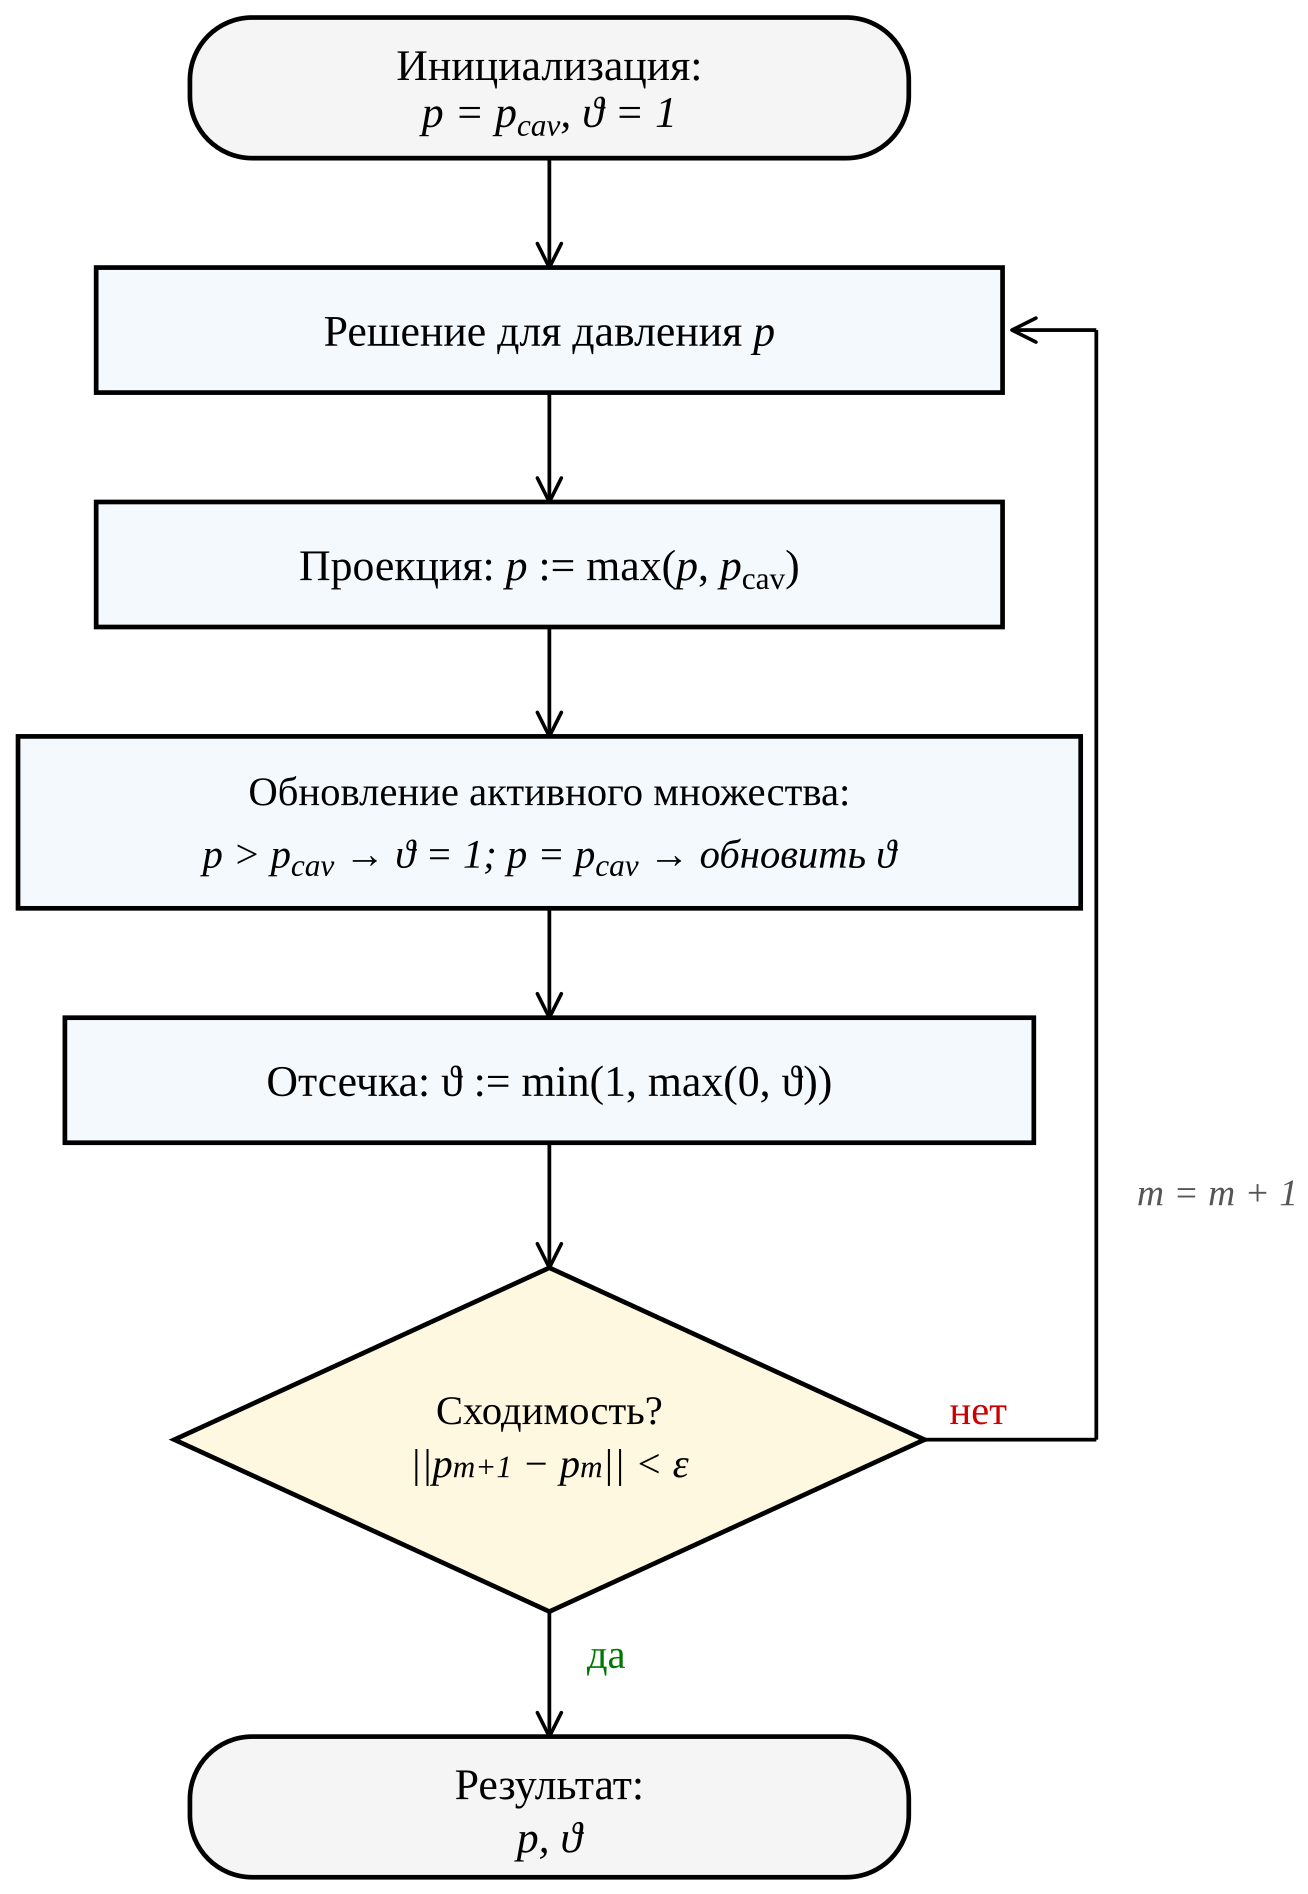
\includegraphics[width=\textwidth,height=0.9\textheight,keepaspectratio]{figures/ch02/fig_2_20.png}
\caption{Блок-схема итерационного алгоритма решения задачи JFO}
\label{fig:jfo_algorithm}
\end{figure}

%% Блок 8: Завершающий абзац
Описанная схема при консервативной аппроксимации потоков обеспечивает
массосохраняющее решение задачи кавитации~\cite{elrod1975,meng2017}
и применяется далее ко всем рассматриваемым постановкам (упорный,
радиальный и возвратно-поступательный подшипники).  Подробности
реализации, включая аппроксимацию потоков на гранях ячеек, выбор
солвера и диагностику баланса массы, приведены в главе~3.


% \FloatBarrier
% \FloatBarrier
\section*{Выводы по главе 2}
\phantomsection\addcontentsline{toc}{section}{Выводы по главе 2}

В главе~2 сформулирована единая математическая основа для численного
моделирования смазочного слоя в подшипниках скольжения как для гладкой,
так и для детерминированно микроструктурированной рабочей поверхности.

\begin{enumerate}[wide, labelindent=\parindent, nosep]
  \item Для трёх типовых постановок (упорной, радиальной
    и возвратно-поступательной) введены согласованные поверхностные
    координаты, масштабы безразмеризации и унифицированная форма
    уравнения Рейнольдса, что обеспечивает сопоставимость результатов
    и возможность переноса алгоритмов между постановками.
  \item Сформулирована параметрическая модель детерминированного
    микрорельефа в виде добавки к базовой функции зазора:
    $h = h_{\mathrm{base}} + \Delta h$, где $\Delta h$ задаётся суммой
    вкладов локализованных элементов.  Введены основные геометрические
    параметры элемента (глубина~$h_p$, полуоси~$a$, $b$,
    ориентация~$\alpha$, параметр плоского дна~$\rho_0$,
    длина канавок~$\ell$).
  \item Систематизированы типы геометрии микроструктур
    (эллипсоидальная, параболическая, коническая, косинусная, smoothstep,
    с плоским дном -- для эллиптических элементов; поперечный
    и продольный профили -- для канавок).
    Описаны типы раскладки элементов на поверхности (прямоугольная,
    шахматная, гексагональная, спиральная по принципу филлотаксиса,
    а также раскладка канавок) и сформулировано правило включения
    элементов в область текстурирования.
  \item Введён компактный набор безразмерных параметров микрорельефа
    ($H_p$, $A^{*}$, $B^{*}$, $\kappa$, $P_1^{*}$, $P_2^{*}$, $\phi$,
    $\rho_0$, $\ell^{*}$), позволяющий проводить параметрические
    исследования и сравнивать различные конфигурации при одинаковых
    безразмерных параметрах.
  \item Рассмотрена физическая природа кавитации и показаны ограничения
    инженерного подхода отсечения давления снизу (условие Гюмбеля),
    связанные с нарушением баланса массы.  Для корректного учёта разрыва
    плёнки сформулирована массосохраняющая постановка кавитации (JFO),
    включающая уравнение
    сохранения для~$\vartheta h$ и условия комплементарности
    для~$p$ и~$\vartheta$.
  \item Описана связь постановки JFO с численной реализацией:
    дискретизация в консервативной форме и итерационное решение методом
    активного множества.  Подробности дискретизации потоков, выбора
    решателя и проверки массобаланса вынесены в главу~3.
\end{enumerate}

Сформулированные модели, параметризация микрорельефа и массосохраняющая
модель кавитации (JFO) образуют основу для реализации расчётного алгоритма
и проведения вычислительных экспериментов, представленных в последующих
главах.


\FloatBarrier
\section*{Контрольные вопросы}
\phantomsection\addcontentsline{toc}{section}{Контрольные вопросы}

\begin{enumerate}
\item Из~каких уравнений выводится уравнение Рейнольдса?
\item Какие допущения используются при~выводе уравнения Рейнольдса?
\item Как~записывается уравнение Рейнольдса для~плоскопараллельной задачи (упорный подшипник)?
\item В~чём отличие постановки задачи для~радиального и~упорного подшипников?
\item Как~учитывается геометрия микрорельефа в~функции зазора?
\item Какие схемы расположения элементов микрорельефа существуют (кольцевое, шахматное, филлотаксис)?
\item Что~такое безразмеризация и~зачем она~применяется?
\item Что~такое модель JFO и~какую проблему она~решает?
\item Как~формулируются граничные условия при~кавитации?
\item Какие функционалы используются для~оценки характеристик подшипника?
\item Что~такое условия комплементарности в~постановке JFO?
\item В~чём состоит конкуренция двух гидродинамических эффектов при~текстурировании поверхности?
\end{enumerate}
       % Глава 2: Постановка и моделирование
\chapter{Численное моделирование гидродинамических задач смазочного слоя}

\section{Граничные условия}
Для замыкания дискретной задачи необходимо задать граничные условия на давление~$p$ и (при использовании модели JFO) на степень заполнения~$\vartheta$. Тип граничных условий определяется физической постановкой (подразделы~2.1.2-2.1.4) и геометрией расчётной области. Ниже систематизированы три основных типа граничных условий для давления.

\textit{Дирихле (заданное давление).}
На соответствующем участке границы $\Gamma_D$ давление фиксируется:
\[
  p = p_0 \quad \text{на} \quad \Gamma_D.
\]

Наиболее распространённый случай -- $p_0 = p_{\mathrm{cav}} = 0$ (в избыточных давлениях) на открытых границах расчётной области, где смазочный слой сообщается с окружающей средой. Типичные примеры: торцы по оси~$z$ для радиального подшипника, радиальные границы $r = R_{\mathrm{in}},\, R_{\mathrm{out}}$ для упорного.

\textit{Периодичность.}
По окружному (периодическому) направлению давление совпадает на противоположных границах области:
\[
  p(x_{1,s},\, x_2) = p(x_{1,t},\, x_2).
\]

Данное условие применяется в упорных и радиальных подшипниках, где расчётная область охватывает полный период по окружной координате. При расчёте сектора вместо периодичности на границах сектора задаются условия симметрии ($\partial p / \partial n = 0$) или заданное давление в зависимости от постановки.

\textit{Непроницаемость (Нейман).}
На участках с условием симметрии или непроницаемости нормальная производная давления обращается в нуль:
\[
  \frac{\partial p}{\partial n} = 0 \quad \text{на} \quad \Gamma_N.
\]

Условие $\partial p / \partial n = 0$ эквивалентно отсутствию напорного потока через границу и используется на линиях симметрии или на искусственных границах при расчёте сектора.

В таблице~\ref{tab:bc_summary} сведены граничные условия для давления, соответствующие трём постановкам, сформулированным в подразделах~2.1.2-2.1.4.

\begin{table}[!ht]
\centering
\caption{Граничные условия для давления в различных постановках
  (координаты $x_1$,~$x_2$ определены в подразделах~2.1.6 и~2.2.1)}
\label{tab:bc_summary}
\begin{tabularx}{\textwidth}{|X|c|c|}
\hline
\multicolumn{1}{|c|}{\textbf{Постановка}} & \textbf{По $\boldsymbol{x_1}$}
                       & \textbf{По $\boldsymbol{x_2}$} \\
\hline
Торцевой зазор
  & периодичность
  & $p = p_{\mathrm{cav}}$, $x_2 = r$ \\
\hline
Радиальный зазор при окружном сдвиге
  & периодичность
  & $p = p_{\mathrm{cav}}$, $x_2 = z$ \\
\hline
Радиальный зазор при возвратно-поступательном движении
  & $p = p_{\mathrm{cav}}$, $x_1 = z$
  & периодичность \\
\hline
\end{tabularx}
\end{table}

\FloatBarrier

При использовании массо-сохраняющей модели кавитации JFO (раздел~2.3) дополнительно задаются граничные условия на степень заполнения~$\vartheta$. На границах подачи смазки полагается $\vartheta = 1$ (полное заполнение зазора). По периодическим направлениям степень заполнения периодична, аналогично давлению. На выходных границах с $p = p_{\mathrm{cav}}$ величина~$\vartheta$ явно не фиксируется; она определяется из уравнения сохранения~\eqref{eq:jfo_conservation} и схемы переноса, что соответствует свободному выходу смеси.

Во всех рассматриваемых постановках кавитационное давление принимается равным нулю в избыточных давлениях: $p_{\mathrm{cav}} = 0$.

Перечисленные типы граничных условий по-разному реализуются
в сеточной схеме. Узлы с условием Дирихле исключаются
из итерационного обновления: их значения фиксируются
и при вычислении потоков на соседних гранях используются
как известные. Периодичность по координатe~$s_1$ реализуется
отождествлением узлов на противоположных границах расчётной
области~-- фактически граница «замыкается» в кольцо,
и узел $i = 0$ совпадает с узлом $i = N_1$. Условие
неотрицательности давления ($P \geq 0$, кавитация
Рейнольдса) обеспечивается операцией усечения после каждого
шага SOR: если обновлённое значение оказывается отрицательным,
оно принудительно полагается равным нулю. Это эквивалентно
упрощённому методу активного множества без пересчёта степени
заполнения~$\vartheta$. Для JFO-постановки трактовка
кавитационной границы принципиально иная: граница является
свободной и определяется из условия непрерывности потока;
её поточечное обновление описано в разделе~3.5.

\textit{Физический смысл периодичности и~её~отличие от~искусственных граничных условий.}
Условие периодичности по~окружной координате является не~искусственным техническим приёмом, а~точным отражением физической геометрии задачи. Для~радиального подшипника окружная координата~$\varphi$ пробегает полный период $[0, 2\pi]$, и~давление на~входе в~расчётную область действительно равно давлению на~выходе~-- обе~<<границы>> на~самом деле описывают одно и~то~же физическое сечение. Это отличает условие периодичности от~условий Дирихле или~Неймана, которые описывают реальные физические границы (открытые торцы, стенки). Нарушение условия периодичности (например, замена его~на~условие постоянного давления на~обеих граничных линиях~$\varphi = 0$ и~$\varphi = 2\pi$) привело бы к~существенно неверным результатам, так как~фактически изменило бы топологию задачи.

\textit{Граница кавитации в~JFO-постановке как~свободная граница.}
В~упрощённых моделях кавитации (обнуление давления, модель Гюмбеля) граница кавитации явно не~выделяется: давление просто обнуляется поточечно в~тех~узлах, где оно~оказывается отрицательным. Никакого специального граничного условия на~линии раздела зон не~задаётся~-- эта линия неявно определяется самим алгоритмом обнуления.

В~JFO-постановке граница кавитации является свободной границей в~математическом смысле: её~положение не~фиксируется заранее, а~определяется в~ходе решения как~часть ответа. На~этой границе должны выполняться одновременно два условия: давление равно кавитационному~($p = p_{\mathrm{cav}}$) и~поток массы через границу непрерывен (баланс~\eqref{eq:jfo_couette_balance} из~раздела~3.5). Именно второе условие является дополнительным по~сравнению с~упрощёнными моделями и~обеспечивает выполнение баланса масс. Численно свободная граница отслеживается неявно через обновление активного множества~-- алгоритм, описанный в~разделах~2.3.3 и~3.5,~-- без явного хранения координат линии раздела зон~\cite{hori2002,szeri1998}.


\FloatBarrier
\section{Дискретизация}
Дискретизации подлежат уравнение Рейнольдса (при полном заполнении зазора) и его обобщение JFO~\eqref{eq:jfo_conservation}. В обоих случаях используется консервативная (потоковая) форма записи: для каждой ячейки формулируется баланс потоков через её грани. Такой подход обеспечивает сохранение массы на дискретном уровне и является удобной основой для реализации JFO-условий в кавитационной зоне.

Расчётная область покрывается прямоугольной равномерной сеткой с узлами~$(i,\,j)$ и шагами~$\Delta x_1$,~$\Delta x_2$ (формула~\eqref{eq:jfo_grid} в главе~2). Потоки вычисляются на гранях ячеек: $i \pm 1/2$ по~$x_1$ и $j \pm 1/2$ по~$x_2$. Граничные условия на сетке реализуются в соответствии с разделом~3.1.

Консервативный баланс массы на ячейке~$(i,\,j)$ записывается в виде
\begin{equation}\label{eq:discrete_balance}
  \frac{(\vartheta h)_{i,j}^{n+1} - (\vartheta h)_{i,j}^{n}}{\Delta t}
  + \frac{F_{i+\frac{1}{2},j} - F_{i-\frac{1}{2},j}}{\Delta x_1}
  + \frac{G_{i,j+\frac{1}{2}} - G_{i,j-\frac{1}{2}}}{\Delta x_2}
  = 0,
\end{equation}
\begin{conditions}
$F = F_P + F_C$ -- суммарный поток через грань по~$x_1$ (напорный и переносной);\\
$G = G_P + G_C$ -- аналогичный поток по~$x_2$.
\end{conditions}
При полном заполнении ($\vartheta = 1$) уравнение~\eqref{eq:discrete_balance} сводится к классической дискретизации уравнения Рейнольдса. В стационарной постановке член по времени опускается.

\textit{Напорный (пуазейлевский) поток.}
Коэффициент проводимости определяется как
\[
  K = \frac{h^3}{12\mu}.
\]

Потоки на гранях аппроксимируются центральными разностями:
\begin{equation}\label{eq:flux_poiseuille}
\begin{split}
  &F_{P,\,i+\frac{1}{2},j} = -K_{i+\frac{1}{2},j}\,
    \frac{p_{i+1,j} - p_{i,j}}{\Delta x_1}, \\
  &G_{P,\,i,j+\frac{1}{2}} = -K_{i,j+\frac{1}{2}}\,
    \frac{p_{i,j+1} - p_{i,j}}{\Delta x_2}.
\end{split}
\end{equation}

Коэффициент~$K$ на грани вычисляется усреднением значений в соседних узлах (арифметическое или гармоническое усреднение); при достаточно мелкой сетке различия между арифметическим и гармоническим усреднением, как правило, малы.

\textit{Переносной (куэттовский) поток.}
Для уравнения JFO переносной поток записывается в виде
\begin{equation}\label{eq:flux_couette}
\begin{split}
  &F_{C,\,i+\frac{1}{2},j} = \frac{\vartheta_{\mathrm{up}}\,
    h_{i+\frac{1}{2},j}}{2}\,U_1, \\
  &G_{C,\,i,j+\frac{1}{2}} = \frac{\vartheta_{\mathrm{up}}\,
    h_{i,j+\frac{1}{2}}}{2}\,U_2,
\end{split}
\end{equation}

Значение $\vartheta_{\mathrm{up}}$ выбирается из наветренного узла: при $U_1 \geq 0$ берут $\vartheta_{\mathrm{up}} = \vartheta_{i,j}$, иначе $\vartheta_{\mathrm{up}} = \vartheta_{i+1,j}$; аналогично по~$x_2$: при $U_2 \geq 0$ берут $\vartheta_{\mathrm{up}} = \vartheta_{i,j}$, иначе $\vartheta_{\mathrm{up}} = \vartheta_{i,j+1}$. При полном заполнении ($\vartheta = 1$) множитель~$\vartheta_{\mathrm{up}}$ обращается в единицу. Толщина~$h$ на грани вычисляется арифметическим усреднением. Схема расчётной ячейки с указанием потоков на гранях показана на рисунке~\ref{fig:cell_fluxes}.

\begin{figure}[!ht]
\centering
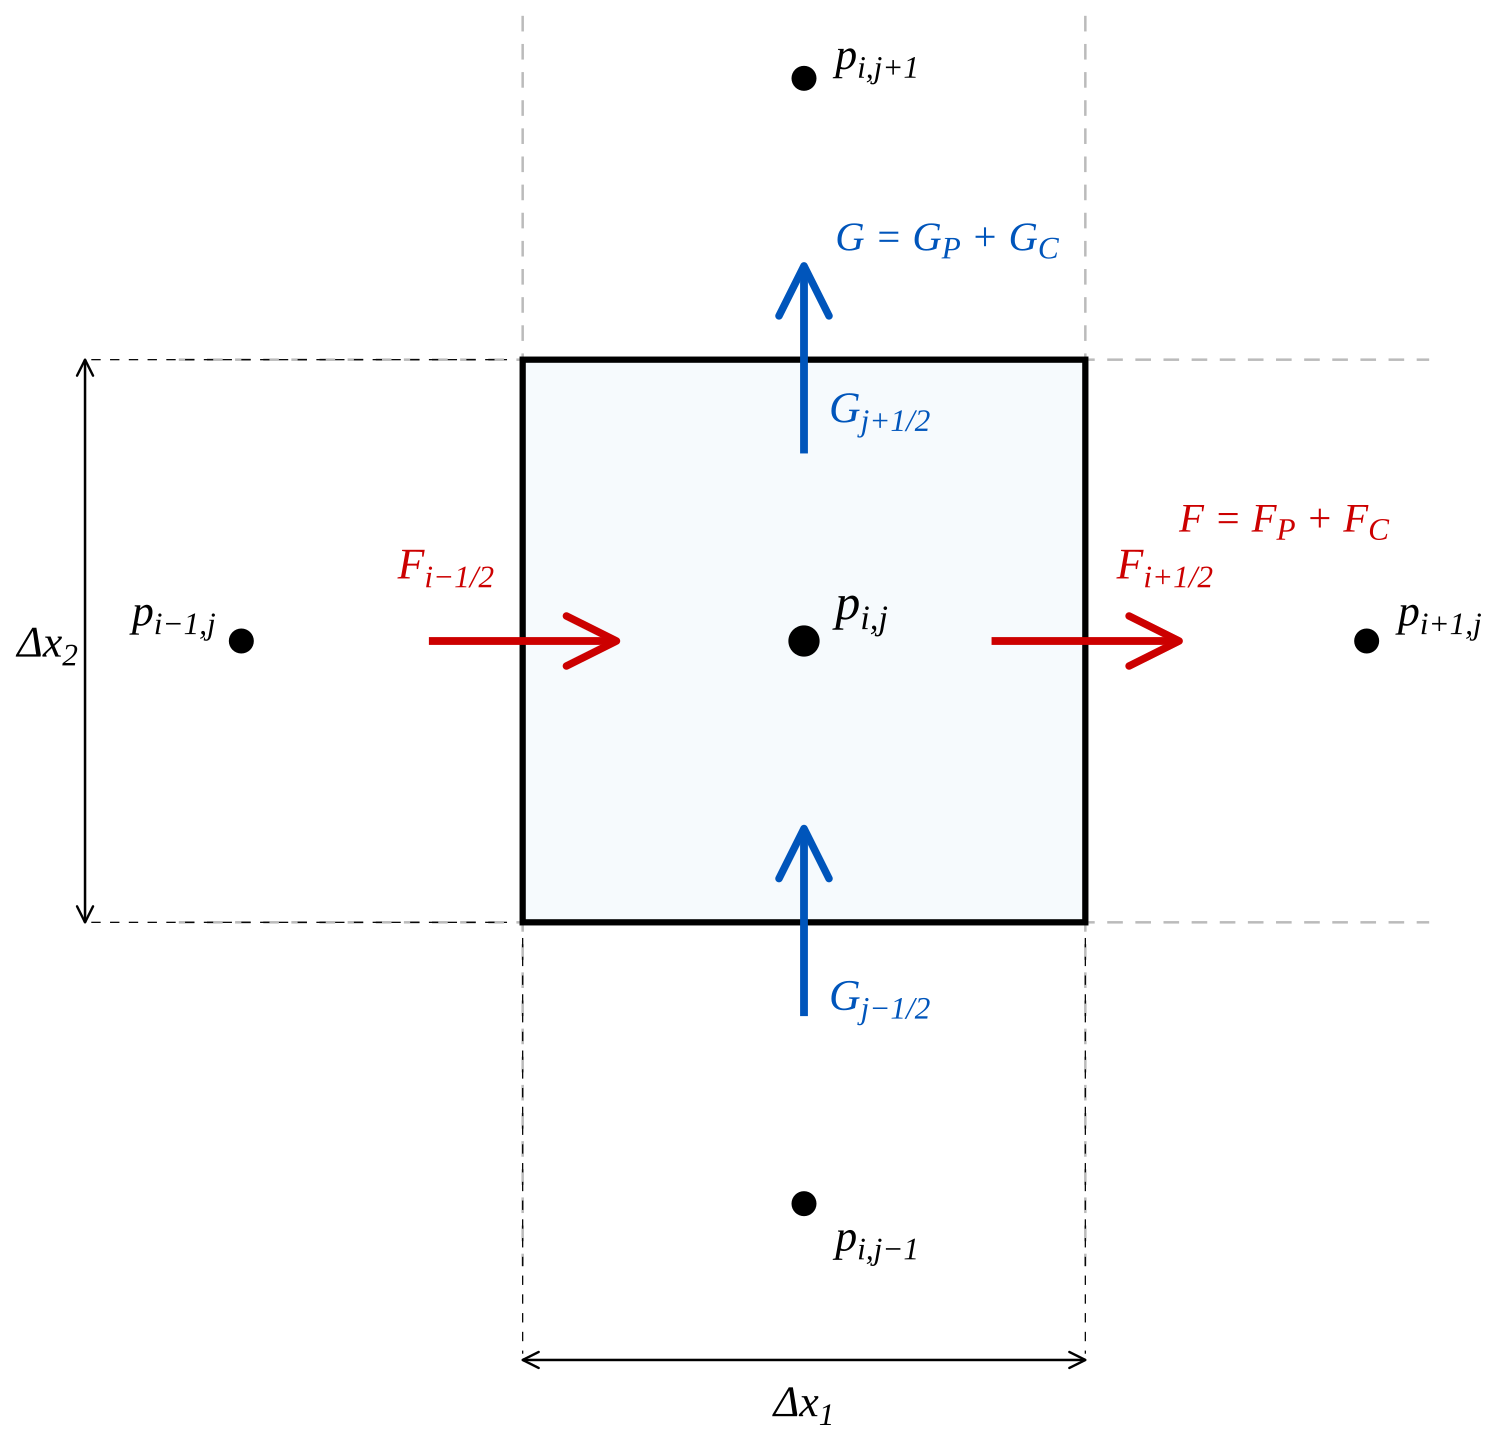
\includegraphics[width=\textwidth,height=0.9\textheight,keepaspectratio]{figures/ch03/fig_3_1.png}
\caption{Схема расчётной ячейки и потоков на гранях}
\label{fig:cell_fluxes}
\end{figure}

\FloatBarrier

\textit{5-точечный шаблон для давления.}
Подстановка потоков в баланс~\eqref{eq:discrete_balance} при $\vartheta = 1$ (стационарный случай) приводит к линейной системе вида
\begin{equation}\label{eq:5point_stencil}
  a_P\,p_{i,j} = a_E\,p_{i+1,j} + a_W\,p_{i-1,j}
    + a_N\,p_{i,j+1} + a_S\,p_{i,j-1} + b_{i,j},
\end{equation}
\begin{conditions}
$a_E$,~$a_W$,~$a_N$,~$a_S$ -- коэффициенты, определяемые проводимостями~$K$ на соответствующих гранях;\\
$a_P = a_E + a_W + a_N + a_S$ -- диагональный коэффициент;\\
$b_{i,j}$ -- правая часть, содержащая вклад куэттовского потока (и, при нестационарности, члена по времени).
\end{conditions}
Система~\eqref{eq:5point_stencil} решается итерационно; выбор решателя описан в разделе~3.3. В нестационарной постановке временной член в~\eqref{eq:discrete_balance} приводит к модификации диагонального коэффициента и правой части разностного уравнения.

В модели JFO давление в кавитационных узлах фиксируется на уровне $p_{\mathrm{cav}}$, поэтому $\nabla p = 0$ и напорные потоки в кавитационной зоне отсутствуют. Обновление активного множества и вычисление~$\vartheta$ в кавитации описаны в разделе~3.5.

Центральные разности для напорного потока обеспечивают второй порядок аппроксимации. Upwind-схема для переноса~$\vartheta$ имеет первый порядок, однако гарантирует устойчивость при доминировании конвективного переноса.

\textit{Порядок аппроксимации и влияние сетки.}
Центральные разности для напорного
потока~\eqref{eq:flux_poiseuille} обеспечивают второй порядок
аппроксимации по $\Delta x_1$, $\Delta x_2$ в узлах, где
зазор $h$ гладко изменяется. В области детерминированных
микроструктур поверхности зазор имеет резкие перепады
на границах элементов рельефа: на переднем склоне лунки $h$
возрастает, на заднем убывает на масштабе нескольких ячеек
сетки. В таких зонах локальный порядок аппроксимации снижается
до первого. Практическое следствие: для корректного
воспроизведения гидродинамического эффекта отдельного элемента
микрорельефа требуется не менее 8--10 узлов на один элемент
вдоль каждого направления. При недостаточном разрешении
коэффициент проводимости~$K_{i+1/2,\,j} =
h_{i+1/2,\,j}^3/(12\mu)$ на грани между «лункой»
и «площадкой» усредняется избыточно, что занижает контраст
потоков и уменьшает расчётный гидродинамический эффект.

\textit{Особенности схемы для цилиндрических координат.}
Для упорного подшипника расчётная область задаётся
в цилиндрических координатах $(r,\,\theta)$. Уравнение
Рейнольдса в этих координатах содержит дополнительные
множители $r$ (перед радиальным потоком) и $1/r$ (перед
угловым): характерные коэффициенты проводимости принимают вид
$K_{r} = r\,h^3/(12\mu)$ и $K_\theta = h^3/(12\mu\,r)$.
В консервативной форме~\eqref{eq:discrete_balance} это
приводит к тому, что коэффициенты~$a_E$, $a_W$ по радиальному
направлению пропорциональны $r_{i+1/2}$ и $r_{i-1/2}$
соответственно, тогда как $a_N$, $a_S$ по угловому делятся
на $r_i$. Структура пятиточечного
шаблона~\eqref{eq:5point_stencil} сохраняется, изменяются
только численные значения коэффициентов.
Правая часть~$b_{i,j}$ включает куэттовский вклад от поворота
диска и согласована с нестационарным членом при наличии
squeeze-эффекта~\cite{han2016,panday2012}.


\FloatBarrier
\section{Итерационные решатели}
Дискретизация уравнения Рейнольдса (раздел~3.2) при полном заполнении зазора ($\vartheta = 1$, стационарный случай) приводит к линейной системе~\eqref{eq:5point_stencil} с пятиточечным шаблоном. Матрица этой системы разреженная; для внутренних узлов каждая строка содержит не более пяти ненулевых коэффициентов (5-точечный шаблон). Число неизвестных определяется числом внутренних узлов сетки~$N_1 \times N_2$. Коэффициенты $a_E$,~$a_W$,~$a_N$,~$a_S$ неотрицательны, поскольку проводимость $K = h^3/(12\mu) > 0$, а диагональное преобладание $a_P = a_E + a_W + a_N + a_S$ обеспечивает благоприятные свойства системы и способствует сходимости стационарных итерационных методов. Прямые методы (например, LU-разложение) для больших сеток неэффективны из-за заполнения разреженной структуры, поэтому используются итерационные методы, допускающие поточечное обновление.

\textit{Метод Гаусса–Зейделя.}
Метод Якоби (одновременное обновление всех узлов по значениям предыдущей итерации) для уравнения Рейнольдса практически не применяется из-за медленной сходимости; его естественное улучшение~-- метод Гаусса–Зейделя. Формула обновления имеет вид
\begin{equation}\label{eq:gs_update}
  p_{i,j}^{(m+1)} = \frac{1}{a_P}\bigl(
    a_E\,p_{i+1,j}^{(m)} + a_W\,p_{i-1,j}^{(m+1)}
    + a_N\,p_{i,j+1}^{(m)} + a_S\,p_{i,j-1}^{(m+1)}
    + b_{i,j}\bigr),
\end{equation}
\noindent где верхний индекс~$(m)$~-- номер итерации. При последовательном обходе сетки по строкам значения $p_{i-1,j}$ и $p_{i,j-1}$ уже обновлены на текущей итерации (индекс~$m+1$), что ускоряет сходимость по сравнению с методом Якоби. Узлы с условиями Дирихле не обновляются~-- их значения фиксированы (раздел~3.1). Периодичность учитывается связыванием пар узлов на противоположных границах расчётной области.

\textit{Последовательная верхняя релаксация (SOR).}
Для ускорения сходимости вводится параметр релаксации~$\omega$. Обновление выполняется в два шага:
\begin{equation}\label{eq:sor_update}
\begin{split}
  &\tilde{p}_{i,j} = \frac{1}{a_P}\bigl(
    a_E\,p_{i+1,j}^{(m)} + a_W\,p_{i-1,j}^{(m+1)}
    + a_N\,p_{i,j+1}^{(m)} + a_S\,p_{i,j-1}^{(m+1)}
    + b_{i,j}\bigr), \\
  &p_{i,j}^{(m+1)} = p_{i,j}^{(m)}
    + \omega\bigl(\tilde{p}_{i,j} - p_{i,j}^{(m)}\bigr).
\end{split}
\end{equation}

При $\omega = 1$ метод совпадает с Гаусса–Зейделя. При $1 < \omega < 2$ выполняется верхняя релаксация (over-relaxation), ускоряющая сходимость. Оптимальное значение~$\omega$ зависит от размера сетки и коэффициентов системы; для задач смазочного слоя типичный диапазон составляет $\omega \in [1{,}2;\; 1{,}9]$, и на практике параметр подбирается эмпирически.

\textit{Критерий сходимости.}
Итерационный процесс останавливается при выполнении одного из двух критериев. Относительная поправка:
\begin{equation}\label{eq:convergence_change}
  \delta^{(m)} = \frac{\displaystyle\sum_{i,j} \bigl|p_{i,j}^{(m+1)} - p_{i,j}^{(m)}\bigr|}
       {\displaystyle\sum_{i,j} \bigl|p_{i,j}^{(m+1)}\bigr| + \varepsilon_0} < \varepsilon,
\end{equation}
\begin{conditions}
$\sum_{i,j}$ -- суммирование ведётся по узлам, в которых давление является неизвестным;\\
$\varepsilon_0$ -- малая добавка для предотвращения деления на нуль (например, $\varepsilon_0 = 10^{-8}$).
\end{conditions}
Невязка разностного уравнения (вычисляется по внутренним узлам):
\begin{equation}\label{eq:convergence_residual}
\begin{split}
  &r_{i,j}^{(m)} = a_P\,p_{i,j}^{(m)} - a_E\,p_{i+1,j}^{(m)} - a_W\,p_{i-1,j}^{(m)}
    - a_N\,p_{i,j+1}^{(m)} - a_S\,p_{i,j-1}^{(m)} - b_{i,j}, \\
  &\max_{i,j}\bigl|r_{i,j}^{(m)}\bigr| < \varepsilon_r.
\end{split}
\end{equation}

Первый критерий (относительная поправка) проще в реализации и используется в данной работе; второй (невязка) не зависит от параметра релаксации и может применяться как дополнительная проверка. Для снижения накладных расходов проверка сходимости выполняется не на каждой итерации, а с заданным интервалом (например, каждые 500~итераций).

\textit{Инициализация и начальное приближение.}
Простейший вариант~-- нулевое начальное поле давления: $p^{(0)}_{i,j} = 0$. При параметрических расчётах (серия задач с постепенно меняющимися параметрами) в качестве начального приближения используется решение предыдущего шага («тёплый старт»), что существенно сокращает число итераций. Аналогично для нестационарных задач начальным приближением служит решение предыдущего временного шага.

\textit{Вычислительная сложность.}
Стоимость одной итерации составляет $O(N_1 N_2)$ операций (одно обновление на узел). Число итераций до сходимости растёт с размером сетки; для типичных сеток $500 \times 500$ может потребоваться $10^3$-$10^4$~итераций.

Последовательный метод Гаусса–Зейделя (и классический SOR) не допускают параллелизма: обновление узла зависит от уже обновлённых соседей. Параметры итерационного процесса, используемые в данной работе, сведены в таблице~\ref{tab:solver_params}. Для преодоления ограничения на параллелизм применяется шахматная (Red-Black) раскраска сетки, позволяющая обновлять половину узлов одновременно; GPU-реализация этого подхода описана в разделе~3.4.

\begin{table}[!ht]
\centering
\caption{Параметры итерационного процесса}
\label{tab:solver_params}
\begin{tabularx}{\textwidth}{|X|c|}
\hline
\multicolumn{1}{|c|}{\textbf{Параметр}} & \textbf{Значение / диапазон} \\
\hline
Метод               & SOR (Гаусс–Зейдель при $\omega = 1$) \\
Релаксация $\omega$ & $1{,}0$-$1{,}9$ (подбирается эмпирически) \\
Критерий остановки  & относительная поправка $\delta^{(m)} < \varepsilon$ \\
Точность $\varepsilon$ & $10^{-5}$-$10^{-6}$ \\
Интервал проверки   & каждые $10^2$-$10^3$ итераций (типично 500) \\
Макс.\ число итераций & $\leq 50\,000$ (верхняя граница) \\
Инициализация       & $p^{(0)} = 0$ или «тёплый старт» \\
\hline
\end{tabularx}
\end{table}

\FloatBarrier

\textit{Влияние параметра релаксации на сходимость.}
Скорость сходимости SOR критически зависит от выбора
параметра~$\omega$. Теоретически оптимальное значение
определяется спектральным радиусом матрицы итерации Якоби:
$\omega_{\mathrm{opt}} = 2/(1 + \sqrt{1 - \rho^2})$,
где $\rho$~-- спектральный радиус. Для практических задач
смазочного слоя спектральный радиус зависит от размера сетки,
коэффициентов анизотропии ($\Lambda$) и характера зазора;
аналитическое выражение для $\rho$ недоступно. На практике
$\omega$ подбирается следующим образом: для новой конфигурации
проводится несколько пробных расчётов на грубой сетке
с различными $\omega \in [1{,}2;\; 1{,}9]$ и выбирается
значение, минимизирующее число итераций; на мелкой сетке
оптимум, как правило, смещается вверх. Для задач
с микротекстурой, где зазор имеет резкие перепады, типичный
рабочий диапазон $\omega \in [1{,}3;\; 1{,}6]$.
При $\omega \geq 2$ итерационный процесс расходится.

\textit{Роль тёплого старта в параметрических расчётах.}
Значительная часть расчётов в главах 5--8 представляет собой
параметрические серии: $\varepsilon$ меняется с шагом $0{,}1$,
или параметр клина $K$ обходит набор значений. В таких сериях
поле давления $P^{(k-1)}$, полученное при предыдущем значении
параметра, является хорошим начальным приближением для
следующего шага. Тёплый старт снижает число итераций до
сходимости в 3--7 раз по сравнению с нулевым начальным полем,
особенно при малых шагах по параметру. Для расчёта
коэффициентов жёсткости и демпфирования (глава~8), где
требуется многократное решение задачи с близкими геометриями
(возмущение рабочей точки на $\pm\Delta x$ или $\pm\Delta v$),
использование тёплого старта от базового решения снижает
вычислительные затраты аналогично~\cite{sfyris2012,chasalevris2013}.


\FloatBarrier
\section{GPU-реализация методом Red--Black SOR}
Последовательный метод SOR~\eqref{eq:sor_update} не допускает параллелизма: обновление каждого узла зависит от значений, вычисленных для соседних узлов на той же итерации. Современные GPU содержат тысячи вычислительных ядер и эффективны при одновременном выполнении большого числа независимых операций. Для использования этого потенциала необходимо переформулировать итерационный процесс так, чтобы обновления узлов на каждом шаге были независимы. Шахматная (Red-Black) раскраска сетки позволяет достичь этого: на каждом полуходе обновляются узлы только одного цвета, и их обновления не зависят друг от друга. Полученный метод Red-Black SOR сохраняет сходимость классического SOR, но допускает массово-параллельную реализацию.

\textit{Шахматная раскраска сетки.}
Каждому узлу~$(i,\,j)$ присваивается цвет в зависимости от чётности суммы индексов:
\begin{equation}\label{eq:rb_coloring}
  c(i,j) = (i + j) \bmod 2.
\end{equation}

Схема шахматной раскраски в~сравнении с~последовательным обходом
при~обычном SOR приведена на~рисунке~\ref{fig:rb_coloring}.

\begin{figure}[!ht]
\centering
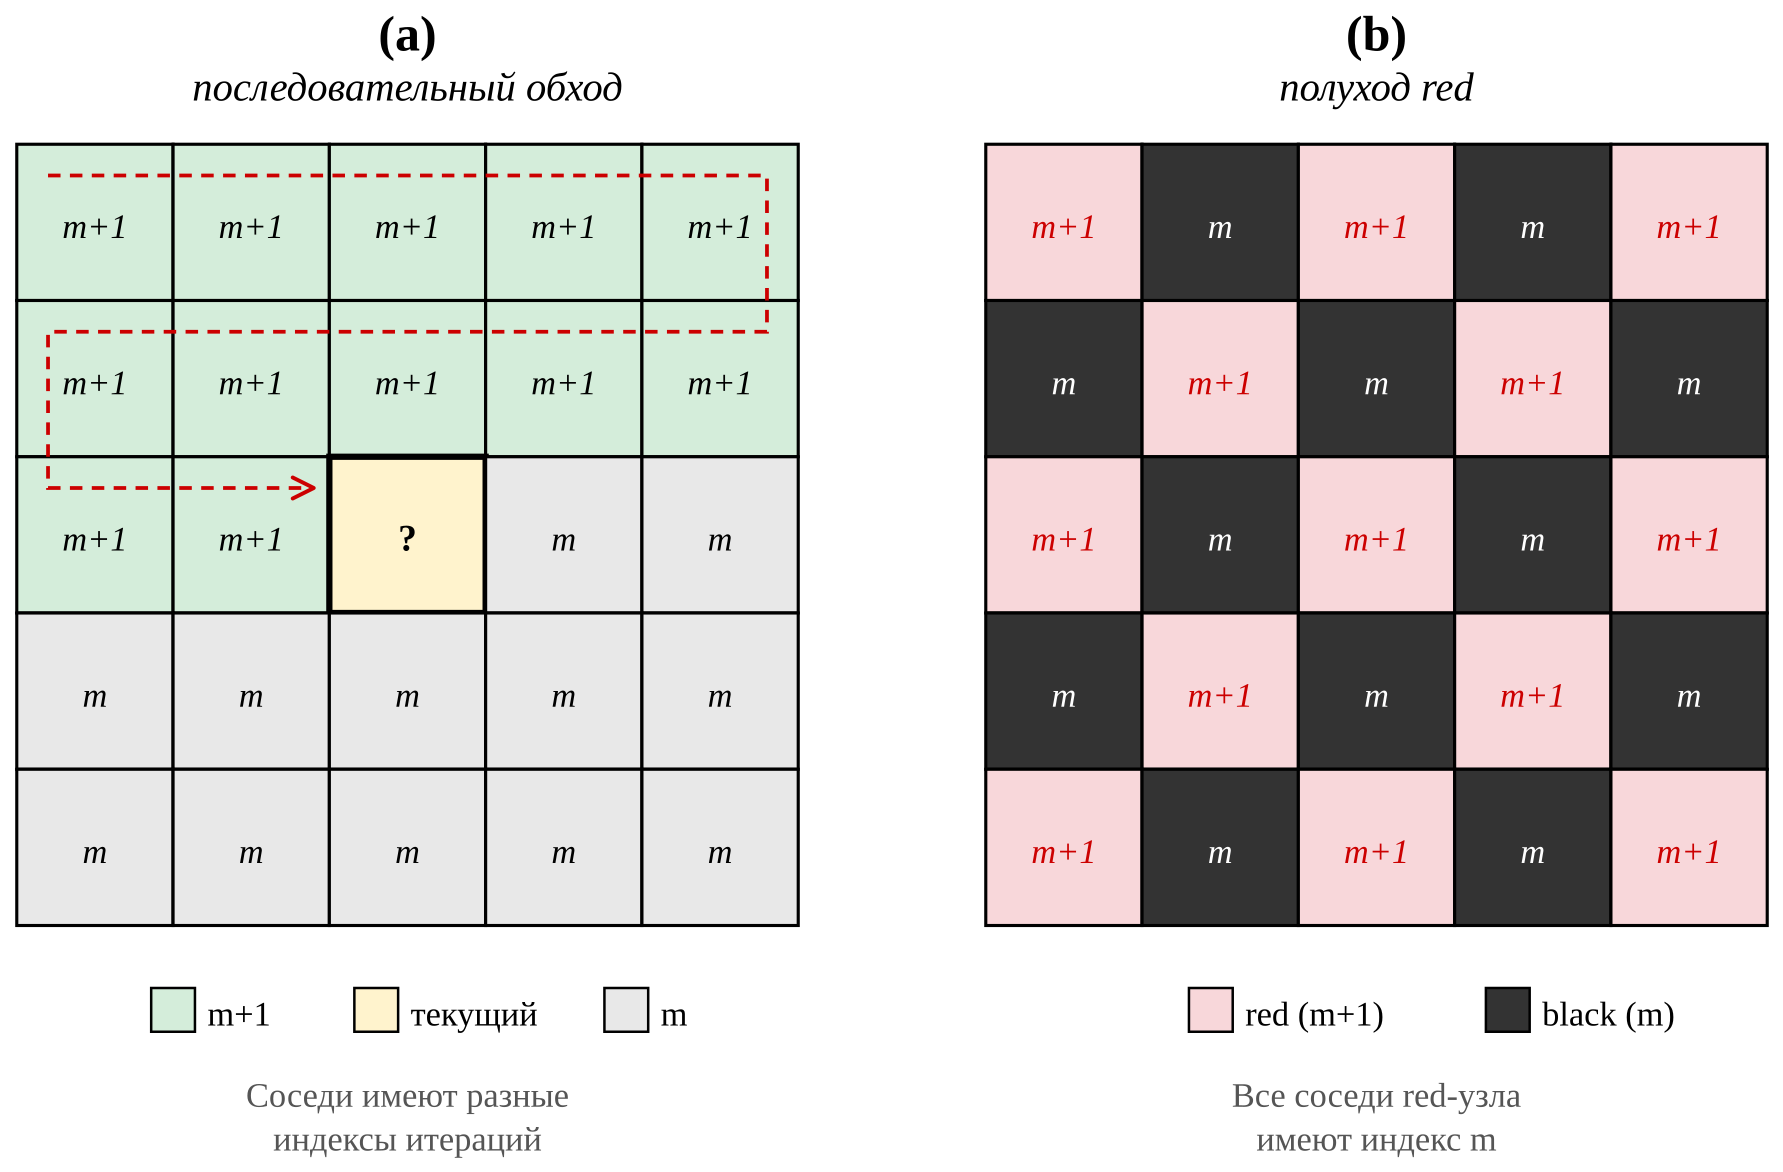
\includegraphics[width=\textwidth,height=0.9\textheight,keepaspectratio]{figures/ch03/fig_3_2.png}
\caption{Сравнение обхода сетки при обычном SOR и шахматной (Red--Black)
раскраске: (а)~последовательный обход по строкам смешивает индексы
итераций; (б)~полуход red обновляет только красные узлы, чёрные соседи
сохраняют индекс~$m$, что обеспечивает независимость обновлений}
\label{fig:rb_coloring}
\end{figure}

\FloatBarrier

Узлы с~$c = 0$ (условно «красные») и~$c = 1$ («чёрные») образуют два непересекающихся подмножества, покрывающих всю сетку. Название связано с аналогией шахматной доски: красные узлы занимают клетки одного цвета, чёрные~-- другого. Ключевое свойство раскраски состоит в том, что в пятиточечном шаблоне~\eqref{eq:5point_stencil} каждый красный узел имеет только чёрных соседей и наоборот. Поэтому при одновременном обновлении всех красных узлов каждый из них использует только значения чёрных соседей, которые не менялись на текущем полуходе,~-- все соседи имеют единый итерационный индекс (на полуходе red~-- индекс~$(m)$, на полуходе black~-- индекс~$(m+\tfrac{1}{2})$, см.\ формулы~\eqref{eq:rb_sor_red}-\eqref{eq:rb_sor_black}). Это свойство делает обновления внутри одного цвета полностью независимыми друг от друга и пригодными для массово-параллельного выполнения: каждый узел может обновляться отдельным потоком GPU без синхронизации с другими потоками. Синхронизация требуется только между полуходами и обеспечивается последовательным запуском ядер GPU: завершение ядра red гарантирует видимость обновлённых значений для ядра black (внутри одного ядра межпоточная синхронизация не требуется). Два полухода составляют одну полную итерацию.

\textit{Обновление давления на полуходе.}
В отличие от классического SOR~\eqref{eq:sor_update}, где часть соседних значений уже обновлена на текущей итерации (индексы~$(m)$ и~$(m+1)$ перемешаны), в Red-Black варианте обновление выполняется в два полухода с чёткой индексацией. На полуходе red обновляются узлы цвета~$c = 0$; их соседи (цвет~$c = 1$) сохраняют значения с итерации~$m$:
\begin{equation}\label{eq:rb_sor_red}
\begin{split}
  &\tilde{p}_{i,j} = \frac{1}{a_P}\bigl(
    a_E\,p_{i+1,j}^{(m)} + a_W\,p_{i-1,j}^{(m)}
    + a_N\,p_{i,j+1}^{(m)} + a_S\,p_{i,j-1}^{(m)}
    + b_{i,j}\bigr), \\
  &p_{i,j}^{(m+1/2)} = p_{i,j}^{(m)}
    + \omega\bigl(\tilde{p}_{i,j} - p_{i,j}^{(m)}\bigr),
    \qquad c(i,j) = 0.
\end{split}
\end{equation}

На полуходе black обновляются узлы цвета~$c = 1$; их соседи (цвет~$c = 0$) уже обновлены на текущей итерации и имеют индекс~$(m+1/2)$:
\begin{equation}\label{eq:rb_sor_black}
\begin{split}
  &\tilde{p}_{i,j} = \frac{1}{a_P}\bigl(
    a_E\,p_{i+1,j}^{(m+1/2)} + a_W\,p_{i-1,j}^{(m+1/2)} + \\
  &+ a_N\,p_{i,j+1}^{(m+1/2)} + a_S\,p_{i,j-1}^{(m+1/2)}
    + b_{i,j}\bigr), \\
  &p_{i,j}^{(m+1)} = p_{i,j}^{(m)}
    + \omega\bigl(\tilde{p}_{i,j} - p_{i,j}^{(m)}\bigr),
    \qquad c(i,j) = 1.
\end{split}
\end{equation}

Внутри каждого полухода все соседи имеют фиксированные значения (противоположный цвет не обновляется), что обеспечивает полную независимость обновлений и пригодность для массово-параллельного выполнения на GPU. Заметим, что на полуходе black релаксация в~\eqref{eq:rb_sor_black} выполняется от~$p_{i,j}^{(m)}$, поскольку чёрные узлы не затрагивались на полуходе red. В ядре обновления при необходимости выполняется проекция~$p \leftarrow \max(p,\, p_{\mathrm{cav}})$. В расчётах в избыточных давлениях обычно~$p_{\mathrm{cav}} = 0$. Проекция используется в режимах расчёта с кавитацией (условие Гюмбеля (half-Sommerfeld), раздел~3.5); в режиме полного заполнения может быть отключена.

\textit{Граничные условия на GPU.}
После каждой полной итерации (полуход red, затем полуход black) выполняется отдельное ядро, применяющее граничные условия из раздела~3.1. Внутренние узлы расположены в диапазоне~$i = 1, \ldots, N_z - 2$, $j = 1, \ldots, N_\varphi - 2$; слои~$j = 0$ и~$j = N_\varphi - 1$ используются как ghost-узлы для реализации периодичности, а строки~$i = 0$ и~$i = N_z - 1$ соответствуют торцевым границам с условиями Дирихле. Периодичность по окружному направлению обеспечивается копированием значений в ghost-узлы на границах: $P[i,\,0] = P[i,\,N_\varphi-2]$, $P[i,\,N_\varphi-1] = P[i,\,1]$. Это гарантирует корректное обращение к соседям при следующем полуходе. Условия Дирихле на торцах по оси~$z$ реализуются установкой давления кавитации: $P[0,\,j] = p_{\mathrm{cav}}$, $P[N_z-1,\,j] = p_{\mathrm{cav}}$. Граничные условия вынесены в отдельное ядро, чтобы не усложнять ветвление в основном ядре обновления. Это также упрощает адаптацию к другим типам граничных условий (например, при расчёте сектора вместо полного кольца). Ядро граничных условий запускается с одномерной сеткой потоков: каждый поток обрабатывает одну строку (для периодичности) или один столбец (для Дирихле).

\textit{Организация вычислений и конфигурация запуска.}
Ядро обновления давления использует двумерную сетку потоков GPU. Блок потоков имеет размер~$32 \times 8$: 32~потока по быстрому (окружному) индексу~$j$ соответствуют одной warp-линии~-- группе потоков, выполняющихся синхронно на одном мультипроцессоре. Такой выбор обеспечивает коалесцированный (последовательный) доступ к глобальной памяти: соседние потоки обращаются к соседним элементам массива, что минимизирует число транзакций памяти. Размер сетки блоков вычисляется из числа внутренних узлов: $(N_\varphi - 2)$ по окружному и $(N_z - 2)$ по осевому направлению. Потоки, попадающие за пределы расчётной области, завершаются без выполнения операций.

Каждый поток обрабатывает один внутренний узел. Поток вычисляет свои индексы~$(i,\,j)$ и проверяет условие раскраски~$c(i,j) = (i+j) \bmod 2$. Если цвет узла не совпадает с текущим полуходом, поток пропускает обновление. Все данные (давление, коэффициенты, правая часть) хранятся в глобальной памяти GPU в формате двойной точности. Коэффициенты дискретизации предварительно вычисляются на GPU из поля зазора~$h$ средствами поэлементных операций.

Ядро граничных условий запускается с одномерной сеткой потоков (блок из 256~потоков). Размер сетки определяется максимумом из~$N_z$ и~$N_\varphi$. Каждый поток обрабатывает либо одну строку (копирование для периодичности), либо один столбец (обнуление для Дирихле).

Коэффициенты дискретизации в реализации обозначаются~$A$, $B$, $C$, $D$, $E$, $F$ и связаны с обозначениями раздела~3.2 соотношениями: $A = a_E$, $B = a_W$, $C = a_N$, $D = a_S$, $E = a_P$, $F = b_{i,j}$.

\textit{Контроль сходимости.}
Сходимость контролируется по критерию относительной поправки~\eqref{eq:convergence_change} из раздела~3.3. Для снижения накладных расходов проверка выполняется не на каждой итерации, а с интервалом (типично~-- каждые несколько сотен итераций, таблица~\ref{tab:solver_params}). Перед началом блока итераций сохраняется копия текущего поля давления в отдельный GPU-буфер. После завершения блока вычисляется~$\delta^{(m)}$ средствами массовых операций GPU: поэлементное вычитание массивов, суммирование модулей разностей и суммирование модулей текущего решения. Эти операции выполняются на GPU без переноса данных на CPU; на CPU передаётся только скалярный результат~$\delta^{(m)}$. При $\delta^{(m)} < \varepsilon$ итерации прекращаются.

Проверка сходимости не на каждой итерации обусловлена тем, что вычисление~$\delta$ требует глобальной редукции (суммирования по всему массиву), которая является синхронной операцией и нарушает конвейер GPU. Выполнение редукции каждые несколько сотен итераций (а не каждую) практически не влияет на точность определения момента сходимости, но существенно снижает накладные расходы.

\textit{Кэширование GPU-буферов.}
При решении серии задач на одной сетке (например, параметрическое варьирование эксцентриситета, угла наклона, глубины микрорельефа) размер массивов не меняется. Выделение и освобождение GPU-памяти~-- дорогостоящие операции; повторное их выполнение на каждом вызове решателя создаёт значительные накладные расходы. Поэтому при первом вызове для данного размера сетки~$N_z \times N_\varphi$ выделяются рабочие буферы (массивы давления, копии для проверки сходимости, массивы коэффициентов дискретизации). При последующих вызовах с тем же размером сетки буферы переиспользуются~-- выполняется только обнуление массива давления и пересчёт коэффициентов. Это особенно эффективно при расчёте характеристик подшипника в диапазоне параметров, когда решатель вызывается десятки и сотни раз подряд.

\textit{Алгоритм итерации.}
На вход подаётся поле зазора~$h_{i,j}$, шаги сетки~$\Delta x_1$, $\Delta x_2$ и геометрические параметры ($R$,~$L$). На первом этапе из поля зазора вычисляются коэффициенты дискретизации~$a_E$, $a_W$, $a_N$, $a_S$, $a_P$ и правая часть~$b_{i,j}$~-- все операции выполняются на GPU. Поле давления инициализируется нулями.

Далее выполняется итерационный цикл. Одна полная итерация состоит из трёх этапов: обновление давления в узлах цвета~$c = 0$ (полуход red), обновление в узлах цвета~$c = 1$ (полуход black), применение граничных условий. С заданным интервалом (типично каждые 500~итераций) перед блоком итераций сохраняется копия поля давления, а после блока вычисляется относительная поправка~$\delta^{(m)}$~\eqref{eq:convergence_change}. Если $\delta^{(m)} < \varepsilon$, итерации прекращаются. Если достигнуто максимальное число итераций, процесс также останавливается с фиксацией достигнутого значения~$\delta$.

По завершении итераций результирующее поле давления переносится из памяти GPU на CPU для дальнейшего вычисления интегральных характеристик (несущая способность, момент трения, утечки; см.\ подраздел <<Целевые функционалы и выходные величины>>)~\cite{ansys2013}.

Описанный GPU-решатель применяется как внутренний решатель линейной системы в алгоритме JFO (раздел~3.5), где дополнительно выполняется обновление активного множества и вычисление степени заполнения~$\vartheta$ в кавитационной зоне.


\FloatBarrier
\section{Реализация модели кавитации JFO}
Теоретическая постановка задачи JFO (уравнение сохранения~\eqref{eq:jfo_conservation}, условия комплементарности~\eqref{eq:jfo_complementarity}) и общая схема итерационного алгоритма active-set приведены в подразделах~2.3.2-2.3.3~\cite{elrod1975}. В настоящем разделе описывается численная реализация каждого шага этого алгоритма: решение подсистемы для давления на GPU (раздел~3.4), обновление степени заполнения~$\vartheta$ в кавитационной зоне, переключение узлов между зонами полного заполнения и кавитации, критерии остановки. Алгоритм JFO имеет двухуровневую итерационную структуру: внутренний цикл~-- решение линейной системы для давления методом Red-Black SOR на GPU при фиксированном~$\vartheta$, внешний цикл~-- обновление активного множества и пересчёт~$\vartheta$.

\textit{Решение подсистемы для давления.}
На каждой внешней итерации~$m$ фиксируется текущее распределение~$\vartheta^{(m)}$. В узлах зоны полного заполнения ($\vartheta = 1$) решается система~\eqref{eq:5point_stencil} методом Red-Black SOR (раздел~3.4) до сходимости по критерию~\eqref{eq:convergence_change}. В узлах зоны кавитации давление фиксировано: $p_{i,j} = p_{\mathrm{cav}}$. Эти узлы не обновляются решателем давления; фиксация обеспечивается проекцией $p \leftarrow \max(p,\, p_{\mathrm{cav}})$, встроенной в ядро обновления (раздел~3.4). В кавитационных узлах давление фиксируется на уровне~$p_{\mathrm{cav}}$, поэтому внутри связной кавитационной области градиенты давления отсутствуют и напорный поток не формируется. На границе кавитации и полного заполнения градиент давления, как правило, отличен от нуля и определяется решением в зоне полного заполнения.

Коэффициенты напорной части дискретизации ($a_E$, $a_W$, $a_N$, $a_S$, $a_P$), определяемые полем зазора~$h$, не зависят от~$\vartheta$ и могут переиспользоваться во внутреннем цикле. Зависимость от~$\vartheta$ проявляется в переносном (куэттовском) потоке~\eqref{eq:flux_couette}, а также в классификации узлов как кавитационных ($p = p_{\mathrm{cav}}$) или полностью заполненных.

\textit{Обновление степени заполнения в кавитационной зоне.}
В кавитационной зоне $p = p_{\mathrm{cav}}$; внутри связной кавитационной области градиенты давления отсутствуют и напорный поток не формируется. Уравнение JFO~\eqref{eq:jfo_conservation} сводится к переносу массы куэттовским потоком. Для стационарной задачи это условие баланса переносных потоков:
\begin{equation}\label{eq:jfo_couette_balance}
  \frac{F_{C,\,i+\frac{1}{2},j} - F_{C,\,i-\frac{1}{2},j}}{\Delta x_1}
  + \frac{G_{C,\,i,j+\frac{1}{2}} - G_{C,\,i,j-\frac{1}{2}}}{\Delta x_2}
  = 0,
\end{equation}
\noindent где переносные потоки на гранях определены в~\eqref{eq:flux_couette} (раздел~3.2):
\begin{equation}\label{eq:jfo_theta_flux}
  F_{C,\,i+\frac{1}{2},j} = \frac{\vartheta_{\mathrm{up}}\,h_{i+\frac{1}{2},j}}{2}\,U_1,
  \quad
  G_{C,\,i,j+\frac{1}{2}} = \frac{\vartheta_{\mathrm{up}}\,h_{i,j+\frac{1}{2}}}{2}\,U_2.
\end{equation}

Значение~$\vartheta_{\mathrm{up}}$ берётся из наветренного узла по направлению скорости~$\mathbf{U}$ (upwind-схема, раздел~3.2). Толщина на грани~-- арифметическое среднее значений в соседних узлах.

В двумерной постановке соотношение~\eqref{eq:jfo_couette_balance} рассматривается как дискретное уравнение переноса для~$\vartheta$. Для наглядности приведём частный случай одномерного переноса по~$x_1$ при~$U_1 > 0$ и отсутствии потоков по~$x_2$, когда баланс упрощается и даёт явную рекуррентную связь:
\begin{equation}\label{eq:jfo_theta_update}
  \vartheta_{i,j} = \frac{\vartheta_{i-1,j}\,h_{i-\frac{1}{2},j}}
    {h_{i+\frac{1}{2},j}}.
\end{equation}

Это соотношение выражает сохранение массы при одномерном переносе: входящий куэттовский поток через грань~$i-1/2$ равен выходящему потоку через грань~$i+1/2$. В двумерном случае баланс~\eqref{eq:jfo_couette_balance} включает потоки по обоим направлениям и реализуется в виде дискретной схемы переноса для~$\vartheta$ (раздел~3.2).

Для нестационарного случая в узлах, отнесённых к кавитационной зоне, используется явная по времени схема (временной шаг~$\Delta t$ из~\eqref{eq:discrete_balance}):
\begin{equation}\label{eq:jfo_theta_transient}
\begin{split}
  &(\vartheta\,h)_{i,j}^{n+1} = (\vartheta\,h)_{i,j}^{n} - {} \\
  &- \Delta t \left[
    \frac{F_{C,\,i+\frac{1}{2},j} - F_{C,\,i-\frac{1}{2},j}}{\Delta x_1}
    + \frac{G_{C,\,i,j+\frac{1}{2}} - G_{C,\,i,j-\frac{1}{2}}}{\Delta x_2}
  \right].
\end{split}
\end{equation}

После обновления выполняется отсечка:
\[
  \vartheta_{i,j} := \min\bigl(1,\;\max(0,\;\vartheta_{i,j})\bigr).
\]

Отсечка обеспечивает физичность решения ($0 \leq \vartheta \leq 1$). Если~$\vartheta_{i,j}$ после обновления достигает единицы, узел переходит в зону полного заполнения на следующей внешней итерации.

\textit{Обновление активного множества.}
После решения подсистемы для давления и проекции $p \leftarrow \max(p,\, p_{\mathrm{cav}})$ каждый узел классифицируется: если $p_{i,j} > p_{\mathrm{cav}} + \varepsilon$, узел принадлежит зоне полного заполнения и~$\vartheta_{i,j} = 1$; если $p_{i,j} \leq p_{\mathrm{cav}} + \varepsilon$, узел принадлежит зоне кавитации и~$\vartheta_{i,j}$ обновляется из баланса переносных потоков~\eqref{eq:jfo_couette_balance}. Малый параметр~$\varepsilon$ (порядка $10^{-6}$-$10^{-8}$ в безразмерном давлении или относительно характерного масштаба давления) необходим для устойчивого определения зоны кавитации и предотвращения осцилляций активного множества на границе зон.

Переключение узлов между зонами~-- это и есть обновление активного множества. Узел может переходить из кавитации в полное заполнение (если~$\vartheta$ достигает~1 или давление вырастает выше~$p_{\mathrm{cav}}$) и обратно (если после проекции выполняется~$p_{i,j} \leq p_{\mathrm{cav}} + \varepsilon$). Процесс продолжается до стабилизации.

\textit{Двухуровневая итерационная структура.}
Внутренний уровень~-- решение линейной системы для давления методом Red-Black SOR на GPU (раздел~3.4) при фиксированном~$\vartheta$. Сходимость внутреннего цикла контролируется по критерию~\eqref{eq:convergence_change} с параметрами из таблицы~\ref{tab:solver_params}. Внешний уровень~-- итерации по активному множеству. На каждой внешней итерации последовательно выполняются: решение для давления (внутренний цикл), проекция~$p \geq p_{\mathrm{cav}}$, обновление активного множества, обновление~$\vartheta$ в кавитационной зоне, отсечка. Общая схема алгоритма приведена в подразделе~2.3.3 (см.\ также рисунок~\ref{fig:jfo_algorithm}).

\textit{Критерии остановки внешнего цикла.}
Внешние итерации прекращаются при одновременном выполнении двух условий: стабилизации активного множества (ни один узел не переключился между зонами на текущей итерации) и малости изменения решения ($\max_{i,j} |p_{i,j}^{(m+1)} - p_{i,j}^{(m)}| < \varepsilon_p$, $\max_{i,j} |\vartheta_{i,j}^{(m+1)} - \vartheta_{i,j}^{(m)}| < \varepsilon_\vartheta$; критерии сформулированы в подразделе~2.3.3). На практике стабилизация активного множества достигается за 5-20~внешних итераций (в зависимости от задачи), при этом каждая внешняя итерация содержит полный внутренний цикл GPU~SOR.

\textit{Инициализация.}
Начальное приближение: $p^{(0)}_{i,j} = p_{\mathrm{cav}}$, $\vartheta^{(0)}_{i,j} = 1$ (полное заполнение). При параметрических расчётах используется тёплый старт: решение предыдущей задачи как начальное приближение для~$p$ и~$\vartheta$, что существенно сокращает число как внешних, так и внутренних итераций.

Описанная реализация при консервативной аппроксимации потоков обеспечивает массосохраняющее решение задачи кавитации и применяется ко всем рассматриваемым постановкам (упорный и радиальный подшипники, возвратно-поступательная пара). Результаты расчётов приведены в главах~5--7.

\textit{Вычислительная стоимость JFO-реализации.}
Основная вычислительная стоимость JFO-алгоритма складывается из~двух частей. Первая~--- внутренний GPU~SOR-цикл для~решения задачи на~давление~--- по~трудоёмкости аналогична обычному решению уравнения Рейнольдса и~масштабируется как~$O(N_1 N_2)$ на~итерацию. Вторая~--- обновление активного множества и~степени заполнения~$\vartheta$~--- выполняется за~один проход по~сетке и~требует значительно меньших затрат. Суммарная стоимость одного внешнего цикла JFO примерно в~2--3~раза превышает стоимость одного SOR-цикла простой Reynolds-задачи; общее число внешних итераций обычно составляет 10--30. Таким образом, JFO-расчёт оказывается примерно в~20--60~раз дороже, чем~один прогон Reynolds-решателя с~обнулением давления. На~практике это приемлемо для~параметрических расчётов при~использовании тёплого старта.

\textit{Особенности сходимости при~фрагментированной кавитации на~микротекстуре.}
При~текстурированных поверхностях с~большим числом лунок (порядка~50--200 на~расчётную область) кавитационная картина существенно фрагментируется: каждая лунка содержит небольшую собственную кавитационную зону. Это замедляет сходимость внешнего цикла активного множества по~следующей причине: при~инициализации с~полным заполнением алгоритму необходимо последовательно <<выявить>> все~локальные кавитационные участки, причём в~начале итераций граница одной кавитационной зоны может влиять на~соседние через~поле давления. Число внешних итераций в~этом случае может вырастать до~50--100 по~сравнению с~10--15 для~гладкого подшипника. Использование тёплого старта существенно снижает этот эффект: при~близких параметрах кавитационный рисунок от~предыдущего решения уже достаточно близок к~текущему, и~алгоритм сходится за~5--15 внешних итераций.

\textit{Допущение о~фиксированной кавитационной области в~динамике.}
При~расчёте динамических коэффициентов (раздел~4.4, глава~8) для~каждого набора возмущений $(\xi, \eta, \dot\xi, \dot\eta)$ в~принципе необходимо решать полную задачу JFO, в~том числе заново определять границу кавитации. Однако это многократно увеличивает вычислительные затраты. На~практике применяется допущение о~фиксированной кавитационной области (\textit{frozen cavitation}): граница кавитации берётся по~полю равновесного давления~$P_0$ и~при~решении возмущённой задачи не~пересматривается. Это допущение оправдано при~малых амплитудах возмущений~$|\xi|, |\eta| \ll c$ и~обеспечивает разумную точность для~прямых коэффициентов. Для~перекрёстных коэффициентов погрешность может быть заметнее, особенно в~режимах с~обширной кавитационной зоной.

\textit{Вычислительная стоимость JFO-реализации.}
Основная вычислительная стоимость JFO-алгоритма складывается из~двух частей. Первая~--- внутренний GPU~SOR-цикл для~решения задачи на~давление~--- по~трудоёмкости аналогична обычному решению уравнения Рейнольдса и~масштабируется как~$O(N_1 N_2)$ на~итерацию. Вторая~--- обновление активного множества и~степени заполнения~$\vartheta$~--- выполняется за~один проход по~сетке и~требует значительно меньших затрат. Суммарная стоимость одного внешнего цикла JFO примерно в~2--3~раза превышает стоимость одного SOR-цикла простой Reynolds-задачи; общее число внешних итераций обычно составляет 10--30. Таким образом, JFO-расчёт оказывается примерно в~20--60~раз дороже, чем~один прогон Reynolds-решателя с~обнулением давления. На~практике это приемлемо для~параметрических расчётов при~использовании тёплого старта.

\textit{Особенности сходимости при~фрагментированной кавитации на~микротекстуре.}
При~текстурированных поверхностях с~большим числом лунок (порядка~50--200 на~расчётную область) кавитационная картина существенно фрагментируется: каждая лунка содержит небольшую собственную кавитационную зону. Это замедляет сходимость внешнего цикла активного множества по~следующей причине: при~инициализации с~полным заполнением алгоритму необходимо последовательно <<выявить>> все~локальные кавитационные участки, причём в~начале итераций граница одной кавитационной зоны может влиять на~соседние через~поле давления. Число внешних итераций в~этом случае может вырастать до~50--100 по~сравнению с~10--15 для~гладкого подшипника. Использование тёплого старта существенно снижает этот эффект: при~близких параметрах кавитационный рисунок от~предыдущего решения уже достаточно близок к~текущему, и~алгоритм сходится за~5--15 внешних итераций.

\textit{Допущение о~фиксированной кавитационной области в~динамике.}
При~расчёте динамических коэффициентов (раздел~4.4, глава~8) для~каждого набора возмущений $(\xi, \eta, \dot\xi, \dot\eta)$ в~принципе необходимо решать полную задачу JFO, в~том числе заново определять границу кавитации. Однако это многократно увеличивает вычислительные затраты. На~практике применяется допущение о~фиксированной кавитационной области (\textit{frozen cavitation}): граница кавитации берётся по~полю равновесного давления~$P_0$ и~при~решении возмущённой задачи не~пересматривается. Это допущение оправдано при~малых амплитудах возмущений~$|\xi|, |\eta| \ll c$ и~обеспечивает разумную точность для~прямых коэффициентов. Для~перекрёстных коэффициентов погрешность может быть заметнее, особенно в~режимах с~обширной кавитационной зоной.


% \FloatBarrier
% \FloatBarrier
\section*{Выводы по главе 3}
\phantomsection\addcontentsline{toc}{section}{Выводы по главе 3}

В главе~3 описана численная реализация решения задач гидродинамики
смазочного слоя, включая дискретизацию уравнения Рейнольдса,
итерационные методы, GPU-ускорение и реализацию модели кавитации JFO.

\begin{enumerate}[wide, labelindent=\parindent, nosep]
  \item Сформулированы граничные условия для дискретной задачи:
    условия Дирихле ($p = p_{\mathrm{cav}}$) на открытых границах,
    периодичность по окружному направлению (в частности, через ghost-узлы
    в GPU-реализации), условия Неймана при расчёте сектора.
    В реализации граничные условия выделены в отдельный этап.
  \item Выполнена консервативная дискретизация уравнения Рейнольдса
    на основе баланса потоков через грани контрольного объёма.
    Напорные потоки аппроксимированы центральными разностями
    (второй порядок), а переносная часть в постановке JFO
    (перенос $\vartheta$) реализована upwind-схемой первого порядка,
    обеспечивающей устойчивость при доминировании конвективного переноса.
    Дискретизация для давления (при $\vartheta=1$) приводит к линейной
    системе с пятиточечным шаблоном.
  \item Для решения дискретной системы выбран метод последовательной
    верхней релаксации (SOR) как естественное ускорение метода
    Гаусса--Зейделя.  Сформулированы критерии сходимости
    (относительная поправка и невязка разностного уравнения)
    и определены параметры итерационного процесса.
  \item Для преодоления ограничения последовательного SOR
    на параллелизм реализован метод Red-Black SOR на GPU.
    Шахматная раскраска сетки и двухполуходная схема (red/black)
    обеспечивают независимость обновлений внутри полухода, что позволяет
    эффективно использовать массово-параллельную архитектуру GPU.
    Описаны конфигурация запуска ядер, кэширование GPU-буферов для серийных
    расчётов и механизм контроля сходимости с минимальными накладными
    расходами на глобальную редукцию.
  \item Реализован алгоритм решения задачи кавитации JFO
    с двухуровневой итерационной структурой: внутренний цикл
    (GPU Red-Black SOR для давления при фиксированном~$\vartheta$)
    и внешний цикл (обновление активного множества и пересчёт степени
    заполнения~$\vartheta$ из баланса переносных потоков).
    Обновление~$\vartheta$ в кавитационной зоне основано на дискретном
    уравнении переноса куэттовским потоком с upwind-аппроксимацией.
    Реализация при консервативной аппроксимации потоков обеспечивает
    массосохраняющее решение задачи кавитации.
\end{enumerate}

Разработанный вычислительный алгоритм (дискретизация, GPU-решатель, JFO)
применяется ко всем рассматриваемым постановкам (упорный, радиальный
и возвратно-поступательный подшипники) и используется в расчётах,
представленных в последующих главах.


\FloatBarrier
\section*{Контрольные вопросы}
\phantomsection\addcontentsline{toc}{section}{Контрольные вопросы}

\begin{enumerate}
\item Какие граничные условия используются для~уравнения Рейнольдса?
\item В~чём суть метода конечных разностей применительно к~уравнению Рейнольдса?
\item Чем~отличаются итерационные методы Якоби и~Гаусса--Зейделя?
\item Что~такое метод верхней релаксации (SOR) и~как выбирается параметр релаксации?
\item В~чём преимущества GPU-реализации вычислений?
\item Что~такое алгоритм Red--Black SOR и~почему он~подходит для~параллельных вычислений?
\item Как~реализуется модель кавитации JFO в~численной схеме?
\item Какие критерии сходимости используются при~итерационном решении?
\item Что~такое метод тёплого старта и~в~каких случаях он~эффективен?
\item В~чём преимущества консервативной дискретизации для~задач с~кавитацией?
\end{enumerate}
       % Глава 3: Численное моделирование
\chapter{Учёт эффектов в решении задач смазочного слоя с рельефом поверхности}

\section{Нелинейность}
Безразмерное уравнение Рейнольдса~\eqref{eq:reynolds_nondim}
в зоне полного заполнения смазочного слоя линейно по давлению:
коэффициент~$\bar{h}^{\,3}$ зависит только от геометрии
и не содержит неизвестных. При наличии микроструктур
поверхности линейность по $p$ сохраняется, однако
вычислительная сложность задачи существенно возрастает~\cite{miraskari2018a,miraskari2018b}.
Во-первых, локальные перепады зазора в ячейках микрорельефа
создают резкий контраст коэффициентов: кубическая
зависимость~$h^3$ усиливает разницу между глубокими и мелкими
участками зазора, что ухудшает обусловленность дискретной
системы и замедляет сходимость итерационных решателей
(раздел~3.3). Во-вторых, кавитация в зонах расходящегося
зазора порождает негладкие ограничения~-- переключение между
зонами полного заполнения и кавитации, совместное определение
давления~$p$ и степени заполнения~$\vartheta$ через условия
комплементарности~\eqref{eq:jfo_complementarity}. В-третьих,
при определённых условиях плотность смазки зависит от искомого
давления ($\rho = \rho(p)$), что вносит дополнительную, но уже
гладкую нелинейность. Ниже каждый из перечисленных эффектов
рассматривается отдельно.

\textit{Кавитация как источник негладкой нелинейности.}
Физическая природа кавитации и массосохраняющая постановка JFO
подробно описаны в подразделах~2.3.1-2.3.2. Здесь существенно
то, что постановка JFO~-- это задача с условиями
комплементарности~\eqref{eq:jfo_complementarity}: в каждом узле
либо $p > p_{\mathrm{cav}}$ и $\vartheta = 1$, либо
$p = p_{\mathrm{cav}}$ и $\vartheta < 1$, причём граница между
зонами заранее неизвестна. Вместо единой линейной системы
возникает задача с неравенствами, которая решается итеративно
методом активного множества~-- внешний цикл обновляет
классификацию узлов и пересчитывает~$\vartheta$, а внутренний
цикл решает линейную подсистему для давления при
фиксированном~$\vartheta$ (глава~3, раздел~3.5). Такая
двухуровневая итерационная структура требует согласования
критериев остановки обоих уровней.

При гладком зазоре кавитация, как правило, формирует одну
связную область, положение которой стабилизируется за несколько
внешних итераций. Микроструктуры поверхности принципиально
усложняют картину: каждый элемент микрорельефа создаёт
локальный перепад зазора с зоной разрежения на расходящемся
участке. В результате кавитационная область может формироваться
не в виде одной связной зоны, а в виде множества
фрагментированных «островков», привязанных к отдельным ячейкам
микрорельефа. Активное множество узлов
с~$p = p_{\mathrm{cav}}$ становится разрозненным, его
конфигурация чувствительна к разрешению сетки и к критериям
остановки внешних итераций. Ошибка в определении границы
кавитации даже на один узел изменяет баланс потоков в соседних
ячейках, поэтому требуется достаточное разрешение сетки для
описания каждого элемента микрорельефа (не менее нескольких
узлов на ячейку) и ужесточение критериев сходимости внешнего
цикла по сравнению с задачей для гладкого зазора.

\textit{Роль параметра $\Lambda$ и анизотропия задачи.}
Параметр
$\Lambda = L_1/L_2$~\eqref{eq:nondim_Lambda} определяет
соотношение вкладов продольного ($s_1$) и поперечного ($s_2$)
членов в уравнении~\eqref{eq:reynolds_nondim}:
при $\Lambda \ll 1$ вклад второго члена мал и задача
приближается к одномерной по~$s_1$, при $\Lambda \gtrsim 1$
существенно возрастает роль поперечного растекания по~$s_2$
(коэффициент перед соответствующим членом
равен $\Lambda^2$). Для задач с микроструктурами
значение~$\Lambda$ определяет, насколько локальные эффекты
микрорельефа «размываются» потоком в поперечном направлении.
При большом~$\Lambda$ поперечное растекание сглаживает
возмущения давления от отдельных ячеек; при малом~$\Lambda$
эти возмущения концентрируются вдоль~$s_1$ и оказывают более
сильное влияние на результирующее поле давления и границы
кавитации.

Конкретные значения~$\Lambda$ для трёх постановок монографии
следуют из масштабов таблицы~\ref{tab:nondim_scales}.
Для радиального подшипника $L_1 = R$ (окружной масштаб),
$L_2 = L$ (длина подшипника), и значения $\Lambda = R/L$
соответствуют умеренной или сильной анизотропии в зависимости
от геометрии. Для упорного подшипника $L_1 = R$,
$L_2 = R_{\mathrm{out}} - R_{\mathrm{in}}$
и $\Lambda = R/(R_{\mathrm{out}} - R_{\mathrm{in}})$, как
правило, порядка единицы, т.\,е.\ задача квази-изотропна.
Для возвратно-поступательного подшипника $L_1 = L$ (длина
цилиндра), $L_2 = R$ и $\Lambda = L/R$ может быть значительно
больше единицы; это означает усиление вклада поперечного члена
(по $s_2 = R\theta$) в безразмерном
уравнении~\eqref{eq:reynolds_nondim} и повышенные требования
к разрешению по поперечному направлению.

С вычислительной точки зрения анизотропия задачи требует
согласования шагов сетки по~$s_1$ и~$s_2$. При больших
значениях $\Lambda$ вклад производных по~$s_2$ усиливается
коэффициентом~$\Lambda^2$, и недостаточное разрешение
по «слабому» направлению может приводить
к дискретизационным ошибкам, доминирующим в оценке сходимости
и искажающим вычисленные границы кавитационных зон. Разумная
стратегия~-- выбирать отношение
$\Delta s_1/\Delta s_2$ порядка~$\Lambda$, чтобы
безразмерные шаги сетки были сопоставимы.

\textit{Изменение плотности: гладкая нелинейность
$\rho = \rho(p)$.}
В задачах глав~5-7 смазка предполагается несжимаемой
жидкостью, $\rho = \mathrm{const}$, и плотность не входит
в число неизвестных. Вместе с тем существуют ситуации, когда
это допущение неприемлемо: газовая смазка, большие перепады
давления в высоконагруженных узлах, двухфазные режимы
со значительным изменением массового содержания фаз в области
кавитации. Для полноты постановки здесь приводится обобщение
уравнения JFO~\eqref{eq:jfo_conservation} на случай переменной
плотности в размерной форме:
\begin{equation}
  \frac{\partial (\rho\,\vartheta\,h)}{\partial t}
  + \nabla\cdot\!\left(
      -\frac{\rho\,h^3}{12\mu}\,\nabla p
      + \frac{\rho\,\vartheta\,h}{2}\,\mathbf{U}
    \right) = 0,
  \label{eq:jfo_rho_general}
\end{equation}
где плотность~$\rho = \rho(p)$ входит как в член накопления,
так и в напорный и переносной потоки. В отличие от
комплементарности JFO, зависимость~$\rho(p)$ является гладкой
(задаётся уравнением состояния конкретной среды), поэтому результирующая нелинейность также гладкая
и устраняется итерациями Пикара с релаксацией: на каждой
итерации $\rho$ пересчитывается по полю давления предыдущего
шага, после чего решается обновлённая система. Такой подход
совместим с двухуровневой структурой алгоритма JFO
(раздел~3.5) и не требует изменения внутреннего
решателя~-- достаточно обновлять коэффициенты системы перед
очередной внешней итерацией. Следует подчеркнуть, что
в расчётах глав~5-7 данной монографии
$\rho = \mathrm{const}$
и обобщение~\eqref{eq:jfo_rho_general} не используется;
раздел описывает его для полноты постановки.

\textit{Термовязкость и внешние итерации.}
Гладкая нелинейность возникает и при учёте термовязкостных
эффектов: если вязкость зависит от температуры
($\mu = \mu(T)$), а температура в свою очередь определяется
скоростью диссипации в зазоре, то уравнение Рейнольдса
оказывается связано с уравнением энергии. В этом случае задача
теряет линейность по $p$: при фиксированном поле $T$ (а значит,
$\mu = \mu(T)$) уравнение по-прежнему линейно по давлению,
однако $T$ зависит от градиентов давления и скорости, что
требует итерационного согласования. Типичная стратегия~--
внешний цикл Пикара (fixed-point): на каждой итерации сначала
решается уравнение Рейнольдса при фиксированном поле вязкости,
затем из полученного поля скоростей пересчитывается температура
и вязкость, и цикл повторяется до выхода на согласованное
решение. Сходимость внешнего цикла, как правило, линейная;
число итераций составляет 5--20 в зависимости от интенсивности
тепловых эффектов. В изотермической постановке, принятой
в прикладных главах настоящей монографии, внешний цикл
не требуется: уравнение Рейнольдса решается как линейная
задача при фиксированной $\mu = \mu_0 = \mathrm{const}$.

Подводя итог, наиболее принципиальная нелинейность при
моделировании смазочного слоя с микроструктурами~-- кавитация
в постановке JFO, порождающая задачу с условиями
комплементарности и фрагментированным активным множеством.
Параметр~$\Lambda$ характеризует анизотропию уравнения
Рейнольдса и режим растекания, определяя степень влияния
локальных эффектов микрорельефа на общую картину давления
и конфигурацию кавитационных зон. Зависимость $\rho(p)$
представляет собой опциональное обобщение, применяемое при
наличии физических предпосылок; в расчётах глав~5-7
монографии смазка принимается несжимаемой~\cite{jang2002,rebufa2017}.


\FloatBarrier
\section{Температура}
В разделе~4.1 было показано, что основные нелинейности при
моделировании смазочного слоя с микроструктурами связаны
с кавитацией (негладкая нелинейность постановки JFO)
и, при необходимости, с зависимостью плотности от
давления (гладкая нелинейность $\rho(p)$). Температура
вводит ещё одну гладкую нелинейность~-- через зависимость
динамической вязкости от температуры $\mu = \mu(T)$:
при фиксированном поле температур уравнение
Рейнольдса~\eqref{eq:reynolds_full} остаётся линейным
по давлению, однако вязкость в его коэффициентах сама
зависит от неизвестного поля~$T$, определяемого балансом
генерации и отвода теплоты. Изменение вязкости
непосредственно влияет на распределение давления, несущую
способность, утечки, потери на трение и положение границ
кавитации. Для задач с микроструктурами температурные
эффекты приобретают дополнительное значение: локальные
перепады толщины зазора усиливают градиенты скорости сдвига
и, как следствие, вязкостную диссипацию, что может приводить
к формированию областей с существенно повышенной
температурой в зонах микрорельефа. Стратегия монографии
состоит в том, что расчёты глав~5--7 выполняются
в изотермическом приближении ($T = T_0$, $\mu = \mathrm{const}$);
настоящий раздел формулирует постановку термовязкостного
(THD) расширения, применимую в случаях, когда тепловые
эффекты существенны.

\textit{Источники и отвод тепла в смазочном слое.}
Основным источником теплоты в тонком смазочном слое является
вязкая диссипация~-- необратимое преобразование кинетической
энергии сдвигового течения в теплоту. Для оценки порядка
величины достаточно рассмотреть чисто куэттовский профиль
скорости между двумя поверхностями: удельная мощность
диссипации в пересчёте на единицу площади~$q^{+}$ пропорциональна $\mu(T)\,U^2/h$, где
$U$~-- характерная скорость поверхности, $h$~-- толщина
зазора. Поскольку $q^{+}$ обратно пропорционален~$h$,
в зонах минимального зазора (в том числе у краёв ячеек
микрорельефа) диссипация резко возрастает. Отвод теплоты
из слоя осуществляется тремя каналами: во-первых,
теплопроводностью через стенки~-- от смазки к валу
и вкладышу; во-вторых, конвективным переносом теплоты
потоком самой смазки от входной области к выходной;
в-третьих, теплоотдачей от наружных поверхностей подшипника
в окружающую среду. Соотношение этих каналов определяется
конкретной конструкцией и режимом работы; в рамках
настоящего раздела для полноты постановки рассматриваются
все три механизма. Общая схема теплового баланса
представлена на рисунке~\ref{fig:heat_balance}.

\begin{figure}[!ht]
\centering
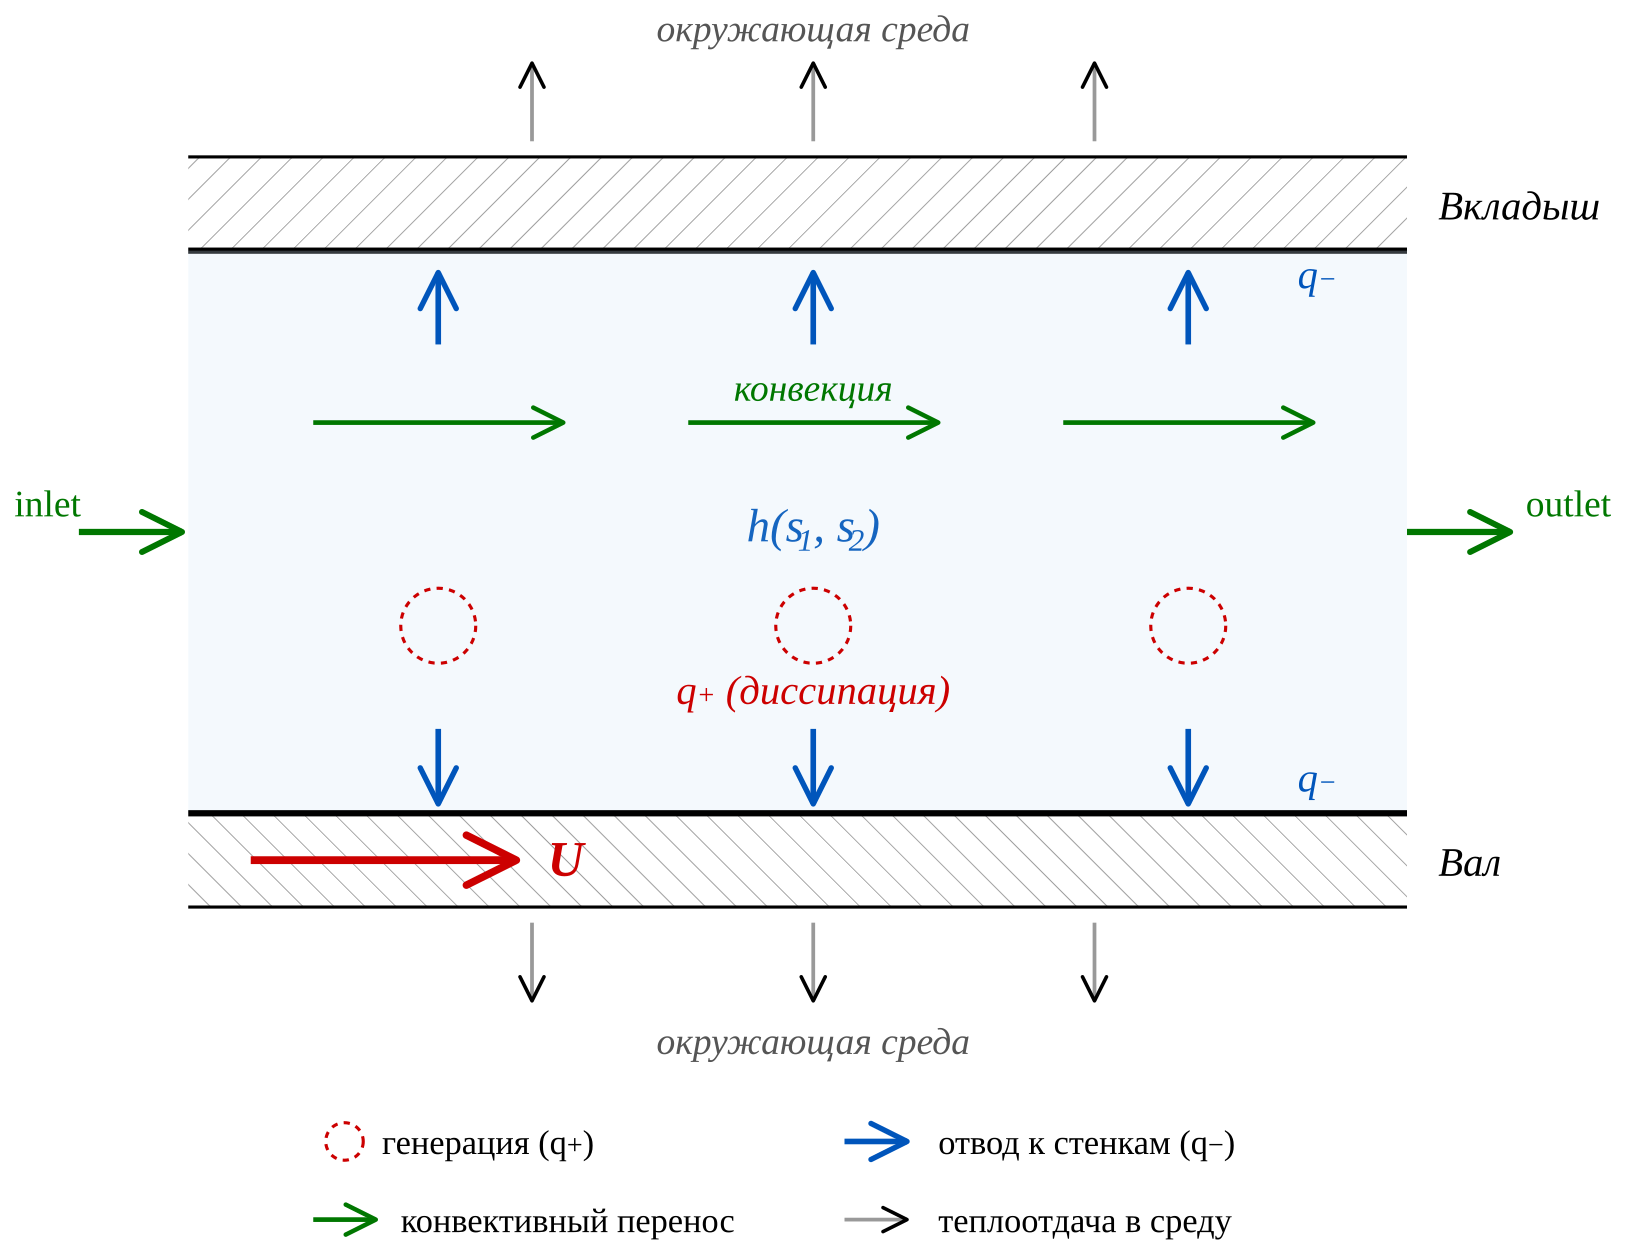
\includegraphics[width=\textwidth,height=0.9\textheight,keepaspectratio]{figures/ch04/fig_4_1.png}
\caption{Источники и каналы отвода теплоты в смазочном слое}
\label{fig:heat_balance}
\end{figure}

\FloatBarrier

\textit{Уровни учёта температуры.}
В зависимости от требуемой точности и вычислительных
ресурсов можно выделить три уровня учёта температуры,
представляющих собой «лестницу сложности» модели.

Первый уровень~-- изотермическое приближение ($T = T_0$,
$\mu = \mu_0 = \mathrm{const}$): температурное поле
не рассчитывается, вязкость принимается постоянной.
Это наиболее простая и распространённая постановка,
используемая в расчётах глав~5--7 настоящей монографии.

Второй уровень~-- приближение эффективной температуры:
сначала решается уравнение Рейнольдса (или задача JFO)
с текущим значением вязкости, затем по полученному полю
давления и скоростей оценивается суммарная диссипация,
вычисляется эффективная температура~$T_{\mathrm{eff}}$
(например, из интегрального теплового баланса), после чего
вязкость обновляется как $\mu(T_{\mathrm{eff}})$
и процедура повторяется до сходимости. Уравнение энергии
в явном виде не решается, что существенно упрощает
реализацию, однако снижает точность при выраженной
неоднородности температурного поля.

Третий уровень~-- термогидродинамика (THD): совместное
решение уравнения Рейнольдса (или задачи JFO) и уравнения
энергии для поля~$T(s_1, s_2, t)$ с учётом зависимости
$\mu(T)$. Этот подход обеспечивает наибольшую точность,
но требует значительных вычислительных затрат, поскольку
на каждой итерации необходимо решать дополнительную краевую
задачу для температуры. Далее в разделе формулируется именно
постановка THD.

\textit{Зависимость вязкости от температуры.}
Для количественного описания влияния температуры
на вязкость необходима аналитическая зависимость $\mu(T)$.
Наиболее употребительным в расчётах тонкоплёночных течений
является экспоненциальный закон:
\begin{equation}
  \mu(T) = \mu_0 \exp\!\bigl(-\beta\,(T - T_0)\bigr),
  \label{eq:viscosity_exp}
\end{equation}
\begin{conditions}
$\mu_0 = \mu(T_0)$ -- вязкость при референсной температуре~$T_0$;\\
$\beta$ -- температурный коэффициент вязкости, $\beta > 0$, K$^{-1}$.
\end{conditions}
При умеренных перепадах температуры (порядка десятков кельвинов)
экспоненциальный закон~\eqref{eq:viscosity_exp} даёт хорошее
приближение и удобен аналитически: производная
$\partial\mu/\partial T = -\beta\,\mu$ линейна по~$\mu$,
что упрощает линеаризацию при итерационном решении.

Для масел в широком диапазоне температур более точным
является трёхпараметрический закон Фогеля:
\begin{equation}
  \mu(T) = A \exp\!\left(\frac{B}{T - C}\right),
  \label{eq:viscosity_vogel}
\end{equation}
\begin{conditions}
$A$, $B$, $C$ -- эмпирические параметры, определяемые
аппроксимацией паспортных данных смазочного масла;\\
$T$ -- абсолютная температура, К.
\end{conditions}
Закон Фогеля~\eqref{eq:viscosity_vogel} лучше описывает
нелинейность кривой $\mu(T)$ при больших температурных
перепадах, однако его параметризация требует экспериментальных
данных. В обоих случаях зависимость $\mu(T)$ является гладкой
и монотонно убывающей~-- повышение температуры приводит
к уменьшению вязкости, что, в свою очередь, снижает несущую
способность и увеличивает утечки, создавая обратную связь
между тепловым и гидродинамическим полями (рисунок~\ref{fig:viscosity_temp}).

\begin{figure}[!ht]
\centering
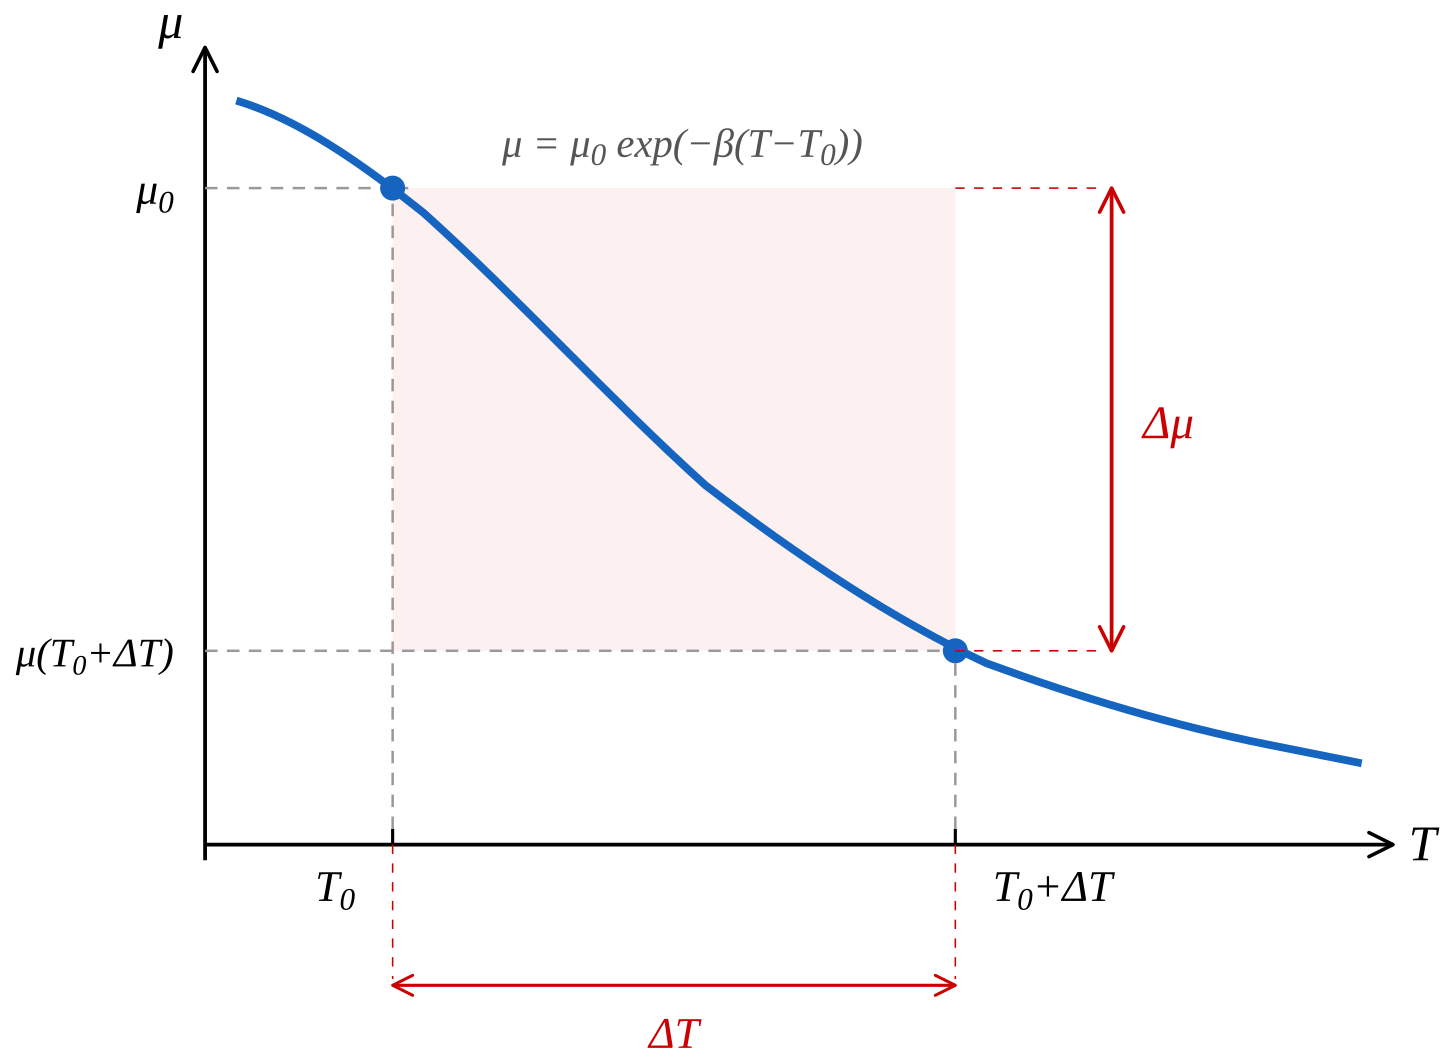
\includegraphics[width=\textwidth,height=0.9\textheight,keepaspectratio]{figures/ch04/fig_4_2.png}
\caption{Типовая температурная зависимость вязкости смазки}
\label{fig:viscosity_temp}
\end{figure}

\FloatBarrier

\textit{Уравнение энергии для смазочного слоя.}
Для описания температурного поля на третьем уровне учёта
(THD) необходимо уравнение энергии. Аналогично тому, как
в разделе~4.1 обобщение JFO с переменной плотностью
записывалось в размерной форме, уравнение энергии здесь
также приводится в размерных переменных. Используется
двумерная плёночная постановка, усреднённая по толщине
зазора:
\begin{equation}
  \rho\,c_p\,h\,\frac{\partial T}{\partial t}
  + \rho\,c_p\,h\,(\mathbf{u}_{\parallel} \cdot \nabla T)
  = \nabla\cdot(k_{\parallel}\,h\,\nabla T)
    + q^{+} - q^{-},
  \label{eq:energy_film}
\end{equation}
\begin{conditions}
$\mathbf{u}_{\parallel}$ -- средняя по толщине скорость
в плоскости $(s_1,\,s_2)$;\\
$c_p$ -- удельная теплоёмкость смазки при постоянном
давлении;\\
$k_{\parallel}$ -- эффективная теплопроводность смазки
в плоскости плёнки;\\
$q^{+}$ -- удельная мощность тепловыделения на единицу площади опорной поверхности, обусловленная вязкой диссипацией; оценка порядка: $q^{+} \sim \mu(T)\,U^2/h$;\\
$q^{-}$ -- удельная мощность теплоотвода на единицу площади к стенкам (валу и вкладышу).
\end{conditions}
Левая часть уравнения~\eqref{eq:energy_film} описывает
нестационарное накопление теплоты и её конвективный перенос
потоком смазки; правая часть~-- диффузию теплоты в плоскости
плёнки, генерацию за счёт диссипации и отвод к ограничивающим
поверхностям.

Средние по толщине скорости $\mathbf{u}_{\parallel}$ вычисляются по стандартным выражениям для тонкого слоя (суперпозиция куэттовского и пуазейлевского профилей) на основе полей $p$, $h$ и $\mu$, полученных на текущей итерации решателя.

\textit{Упрощённая конвективная модель как частный случай.}
В ряде практических постановок общее уравнение
энергии~\eqref{eq:energy_film} допускает существенное упрощение. Ниже приведён вариант для радиальной постановки, где $s_1 = \varphi$~-- окружная координата, $s_2 = Z = z/L$~-- безразмерная осевая координата, $H = h/c_0$~-- безразмерная толщина зазора, $c_0$~-- характерный радиальный зазор подшипника, $P$~-- безразмерное давление в соответствии с безразмеризацией подраздела~2.1.3.
Если принять стационарное приближение ($\partial T/\partial t = 0$),
пренебречь диффузией теплоты в плоскости плёнки
($\nabla\cdot(k_{\parallel}\,h\,\nabla T) \approx 0$) и считать,
что конвективный перенос теплоты осуществляется преимущественно
вдоль окружного направления~$\varphi$,
уравнение~\eqref{eq:energy_film} сводится к конвективной форме. В данной редуцированной постановке теплоотвод к стенкам явно не учитывается (формально $q^{-} \approx 0$); тепловой баланс замыкается конвективным переносом и условием частичного перемешивания на входе~\eqref{eq:bc_partial_mix}:
\begin{equation}
  \mathrm{Pe}\cdot H\,\frac{\partial T}{\partial\varphi}
  = Q_{\mathrm{total}}\cdot\Delta T_{\mathrm{ref}},
  \label{eq:energy_convective}
\end{equation}
где $\mathrm{Pe} = \rho\,c_p\,U\,c_0/k$~-- число Пекле,
характеризующее соотношение конвективного и кондуктивного переноса
теплоты ($k$~-- теплопроводность смазки); $H = h/c_0$~-- безразмерная толщина зазора;
$\Delta T_{\mathrm{ref}}$~-- опорный температурный перепад, используемый при безразмеризации уравнения энергии.
Уравнение~\eqref{eq:energy_convective} является рабочей формой
тепловой модели, реализованной в расчётном модуле.
Уравнение~\eqref{eq:energy_convective} представляет собой ОДУ по~$\varphi$ и решается численным интегрированием по окружности совместно с условием~\eqref{eq:bc_partial_mix}.

Безразмерный источник теплоты~$Q_{\mathrm{total}}$ объединяет вклады
вязкого сдвига (доминирующий) и напорного течения
(пропорциональный~$H^3$):
\begin{equation}
  Q_{\mathrm{total}} = \frac{1}{H}
  + \gamma\,H^3\!\left[
      \left(\frac{\partial P}{\partial\varphi}\right)^{\!2}
      + \left(\frac{D}{L}\right)^{\!2}
        \left(\frac{\partial P}{\partial Z}\right)^{\!2}
    \right],
  \label{eq:Q_total}
\end{equation}
где $P$~-- безразмерное давление; $D$,~$L$~-- диаметр и длина
подшипника; $\gamma$~-- коэффициент, определяемый выбранными
масштабами безразмеризации (в реализованной модели $\gamma = 0{,}1$).
Первое слагаемое~$1/H$ отражает сдвиговую диссипацию Куэтта, второй
член~-- дополнительный вклад пуазейлевской компоненты течения от
градиента давления.

Граничное условие на входе задаётся в виде частичного перемешивания
свежей смазки с нагретой после полного оборота:
\begin{equation}
  T\big|_{\varphi=0}
  = \tfrac{1}{2}\,T_{\mathrm{inlet}}
  + \tfrac{1}{2}\,T\big|_{\varphi=2\pi},
  \label{eq:bc_partial_mix}
\end{equation}
где $T_{\mathrm{inlet}}$~-- температура подаваемой свежей смазки.
Условие~\eqref{eq:bc_partial_mix} моделирует ситуацию, при которой
масло на входе в зазор представляет собой равную смесь свежего масла
и масла, прошедшего полный оборот; в результате эффективная
температура на входе оказывается выше~$T_{\mathrm{inlet}}$, что
соответствует реальному тепловому балансу в подшипнике с непрерывной
циркуляцией смазки.

В полной постановке~\eqref{eq:energy_film} теплоотвод к стенкам задаётся явно через~$q^{-}$; ниже приведены два типовых варианта. При известных температурах стенок используются условия первого рода:
\[
  T_{\mathrm{wall},1} = \mathrm{const}, \qquad
  T_{\mathrm{wall},2} = \mathrm{const},
\]
и~$q^{-}$ определяется из решения поперечного профиля
температуры. Альтернативный, более гибкий подход~-- задание
эффективного конвективного теплоотвода:
\[
  q^{-} = \alpha_1\,(T - T_{\mathrm{wall},1})
         + \alpha_2\,(T - T_{\mathrm{wall},2}),
\]
где $\alpha_1$,~$\alpha_2$~-- коэффициенты теплоотдачи,
определяемые условиями конкретной задачи (геометрией,
теплопроводностью материалов, режимом течения).

Граничные условия для уравнения~\eqref{eq:energy_film}
в плоскости~$(s_1, s_2)$ задаются следующим образом:
на входной границе смазочного слоя температура задана
($T = T_{\mathrm{in}}$), на выходной границе принимается
условие свободного выхода ($\partial T/\partial n = 0$).

\textit{Алгоритм термовязкостного итерационного цикла.}
Совместное решение уравнения Рейнольдса (или задачи JFO)
и уравнения энергии~\eqref{eq:energy_film} с зависимостью
$\mu(T)$ осуществляется итерационно. Структура алгоритма
совместима с двухуровневой схемой решения JFO, описанной
в разделе~3.5: температурный цикл выполняется как
дополнительный внешний уровень, охватывающий циклы
по давлению и кавитации. Последовательность шагов
на каждой итерации~$m$ выглядит следующим образом.
\begin{enumerate}[wide, labelindent=\parindent, nosep]
  \item Задать начальное поле
    $T^{(0)} = T_0$ и вычислить начальную вязкость
    $\mu^{(0)} = \mu(T_0)$.
  \item Решить уравнение Рейнольдса или задачу JFO
    с текущим полем вязкости~$\mu^{(m)}$; получить
    давление~$p^{(m)}$ и поле скоростей.
  \item Решить уравнение энергии~\eqref{eq:energy_film}
    с источником~$q^{+}$, определённым по~$p^{(m)}$
    и~$\mu^{(m)}$; получить обновлённое
    поле~$T^{(m+1)}$.
  \item Применить релаксацию по температуре:
    $T^{(m+1)} \leftarrow (1 - \omega_T)\,T^{(m)}
    + \omega_T\,T^{(m+1)}$,
    где $\omega_T \in (0,\,1]$~-- параметр релаксации;
    после релаксации обновить вязкость:
    $\mu^{(m+1)} = \mu(T^{(m+1)})$ по
    закону~\eqref{eq:viscosity_exp}
    или~\eqref{eq:viscosity_vogel}.
  \item Проверить критерии сходимости; при их выполнении
    остановиться, в противном случае вернуться к шагу~2.
\end{enumerate}

Критерии сходимости формулируются по отклонениям полей
температуры и давления между последовательными итерациями:
\begin{equation}
  \|\,T^{(m+1)} - T^{(m)}\| < \varepsilon_T, \qquad
  \|\,p^{(m+1)} - p^{(m)}\| < \varepsilon_p.
  \label{eq:thd_convergence}
\end{equation}

Параметр релаксации~$\omega_T$ выбирается из условия
устойчивости итераций; при сильной зависимости~$\mu(T)$
(больших значениях~$\beta$ в~\eqref{eq:viscosity_exp})
может потребоваться умеренная подрелаксация
($\omega_T = 0{,}3\text{--}0{,}7$). Важно отметить, что
описанный алгоритм совместим с кэшированием GPU-буферов
(раздел~3.4): при обновлении~$\mu$ на каждой итерации
достаточно пересчитать коэффициенты дискретизации без
переразмещения памяти на устройстве.

\textit{Тепловые эффекты при наличии микроструктур.}
Микроструктуры поверхности существенно модифицируют
тепловую картину смазочного слоя по сравнению с гладким
зазором. Впадины и ячейки микрорельефа создают локальные
зоны с повышенным градиентом скорости сдвига: поскольку
удельная мощность диссипации пропорциональна $\mu\,U^2/h$,
в местах минимального зазора~-- у краёв и на гребнях ячеек~--
источник~$q^{+}$ возрастает резко и нелинейно. При гладком
зазоре диссипация распределена по полю относительно
равномерно; при наличии микротекстур возникают локальные
«горячие пятна», где температура может существенно превышать
среднюю по плёнке (рисунок~\ref{fig:hotspots_texture}).

\begin{figure}[!ht]
\centering
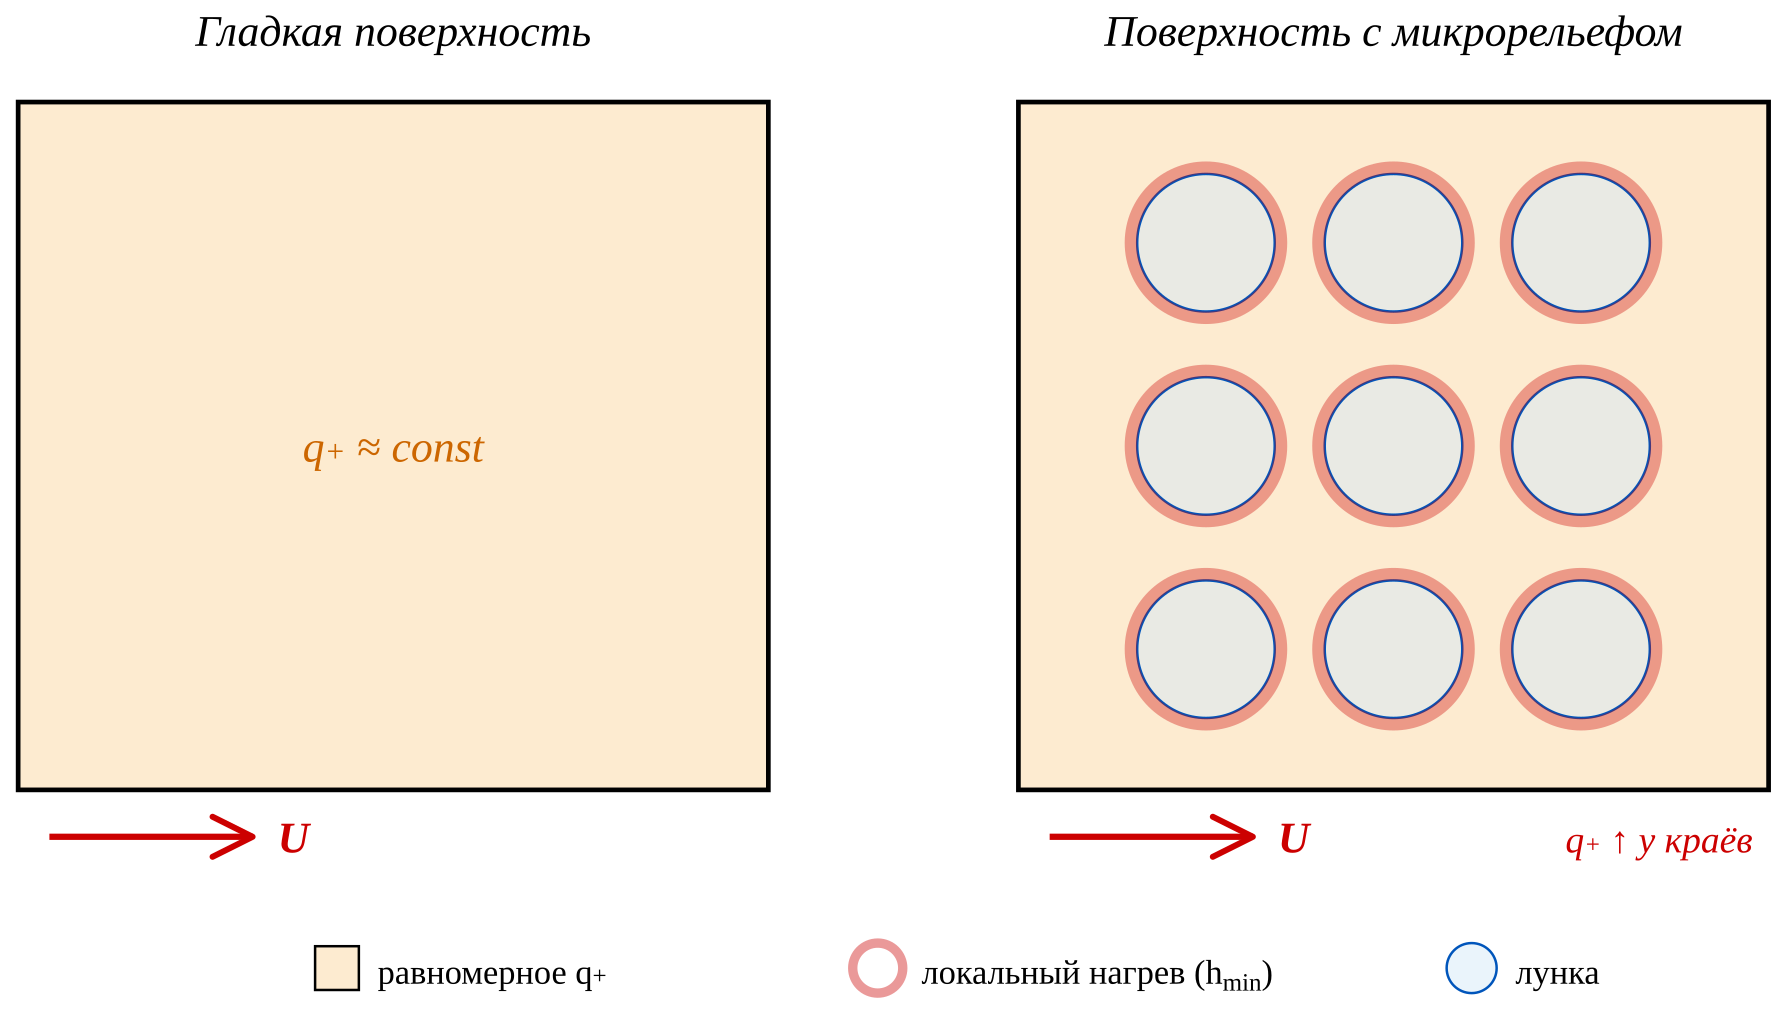
\includegraphics[width=\textwidth,height=0.9\textheight,keepaspectratio]{figures/ch04/fig_4_3.png}
\caption{Локализация диссипации при наличии микротекстур (схема):
  гладкая поверхность (слева) и поверхность с микрорельефом (справа)}
\label{fig:hotspots_texture}
\end{figure}

\FloatBarrier

Это означает, что средняя температура смазочного слоя может
оставаться умеренной, тогда как локальный нагрев в зонах
микрорельефа оказывается значительным и способен повлиять
на несущую способность и границы кавитации. Для корректного
описания таких эффектов необходимо разрешение расчётной
сетки, достаточное для детального представления каждой ячейки
микрорельефа; это требование согласуется с требованиями
по разрешению кавитационных зон, сформулированными
в разделе~4.1. Кавитация (степень заполнения $\vartheta < 1$)
дополнительно модифицирует перенос теплоты в двухфазной
зоне~-- снижение плотности и теплоёмкости газожидкостной
смеси изменяет баланс
уравнения~\eqref{eq:energy_film}; в рамках настоящего
раздела этот эффект детально не раскрывается, однако
представляет собой направление возможного расширения модели.

В расчётах глав~5--7 используется изотермическое
приближение: $T = T_0$, $\mu = \mathrm{const}$. Такой подход
оправдан при умеренных скоростях скольжения и нагрузках, когда
температурный перепад в слое мал и его влияние на вязкость
несущественно. Постановка THD, изложенная
в настоящем разделе, обеспечивает основу для расширения модели
в случаях, когда тепловые эффекты становятся определяющими~--
в частности, при высоких скоростях скольжения, использовании
вязких масел или при глубоких микроструктурах с локально
высокой диссипацией~\cite{kyrkou2020,pierre2004,sun2010,talaighil2015}.


\FloatBarrier
\section{Шероховатость поверхности}
Предметом настоящей монографии являются детерминированные
микроструктуры~-- регулярные элементы заданной геометрии (лунки,
канавки, текстуры), описываемые явным полем добавки~$\Delta h$
в суперпозиции зазора~\eqref{eq:h_superposition} и параметризованные
в подразделе~2.2. Наряду с детерминированным рельефом любая
обработанная поверхность содержит шероховатость~-- случайную
составляющую топографии, возникающую при механической обработке,
полировке или лазерном текстурировании. Шероховатость
характеризуется не явной геометрией, а статистическими параметрами:
среднеарифметическим отклонением профиля~$R_a$,
среднеквадратичным отклонением~$R_q$ и длиной
корреляции~$\lambda_c$. Настоящий раздел устанавливает, при каких
условиях шероховатость существенно влияет на решение задачи
и какие подходы позволяют учесть её при необходимости.

\textit{Критерий значимости шероховатости.}
Определяющим безразмерным параметром является отношение
характерной толщины смазочного слоя~$h_0$ к среднеквадратичной
шероховатости:
\begin{equation}
  \lambda_r = \frac{h_0}{R_q}\,,
  \label{eq:lambda_roughness}
\end{equation}
\begin{conditions}
$h_0$ -- характерная толщина зазора, м;\\
$R_q$ -- комбинированная среднеквадратичная шероховатость
контактирующих поверхностей, м.
\end{conditions}
В задачах с микроструктурами критерием режима служит локальное значение $\lambda_r(s_1, s_2) = h(s_1, s_2)/R_q$; в качестве интегральной оценки режима смазки используют минимальную толщину плёнки~$h_{\min}$, либо характерный минимум~$h_0$.

Параметр~$\lambda_r$ называется числом смазочного слоя
(\textit{film thickness ratio}) и определяет режим взаимодействия
поверхностей. При $\lambda_r \gg 1$ (условно $\lambda_r > 5$)
поверхности надёжно разделены плёнкой смазки, высота
шероховатостей пренебрежимо мала по сравнению с толщиной зазора,
и поле давления определяется макрогеометрией и детерминированным
микрорельефом. При $\lambda_r \approx 1\text{--}3$ высота
микронеровностей становится соизмеримой с толщиной зазора,
шероховатость начинает взаимодействовать с полем давления, и для
адекватного описания потоков требуются модифицированные уравнения.
При $\lambda_r < 1$ реализуется режим граничной смазки
с непосредственным контактом микронеровностей; рейнольдсовская
модель тонкого слоя в этом режиме неприменима.

Для типичных подшипниковых задач с детерминированными
микроструктурами значение~$\lambda_r$ составляет 3--10, что
соответствует режиму гидродинамической смазки. Глубина ячейки
микрорельефа~$h_p = H_p \cdot h_0$ (подраздел~2.2.4,
формула~\eqref{eq:Hp_nondim}) при типичных значениях
$H_p \sim 0{,}1\text{--}1$ существенно превышает амплитуду
шероховатости: $h_p \gg R_q$. Иерархия масштабов~-- базовый
зазор, детерминированная текстура и шероховатость~-- схематически
представлена на рисунке~\ref{fig:roughness_scales}. Это
соотношение масштабов обосновывает допущение о гладкости
поверхностей, принятое в расчётах глав~5--7.

\begin{figure}[!ht]
\centering
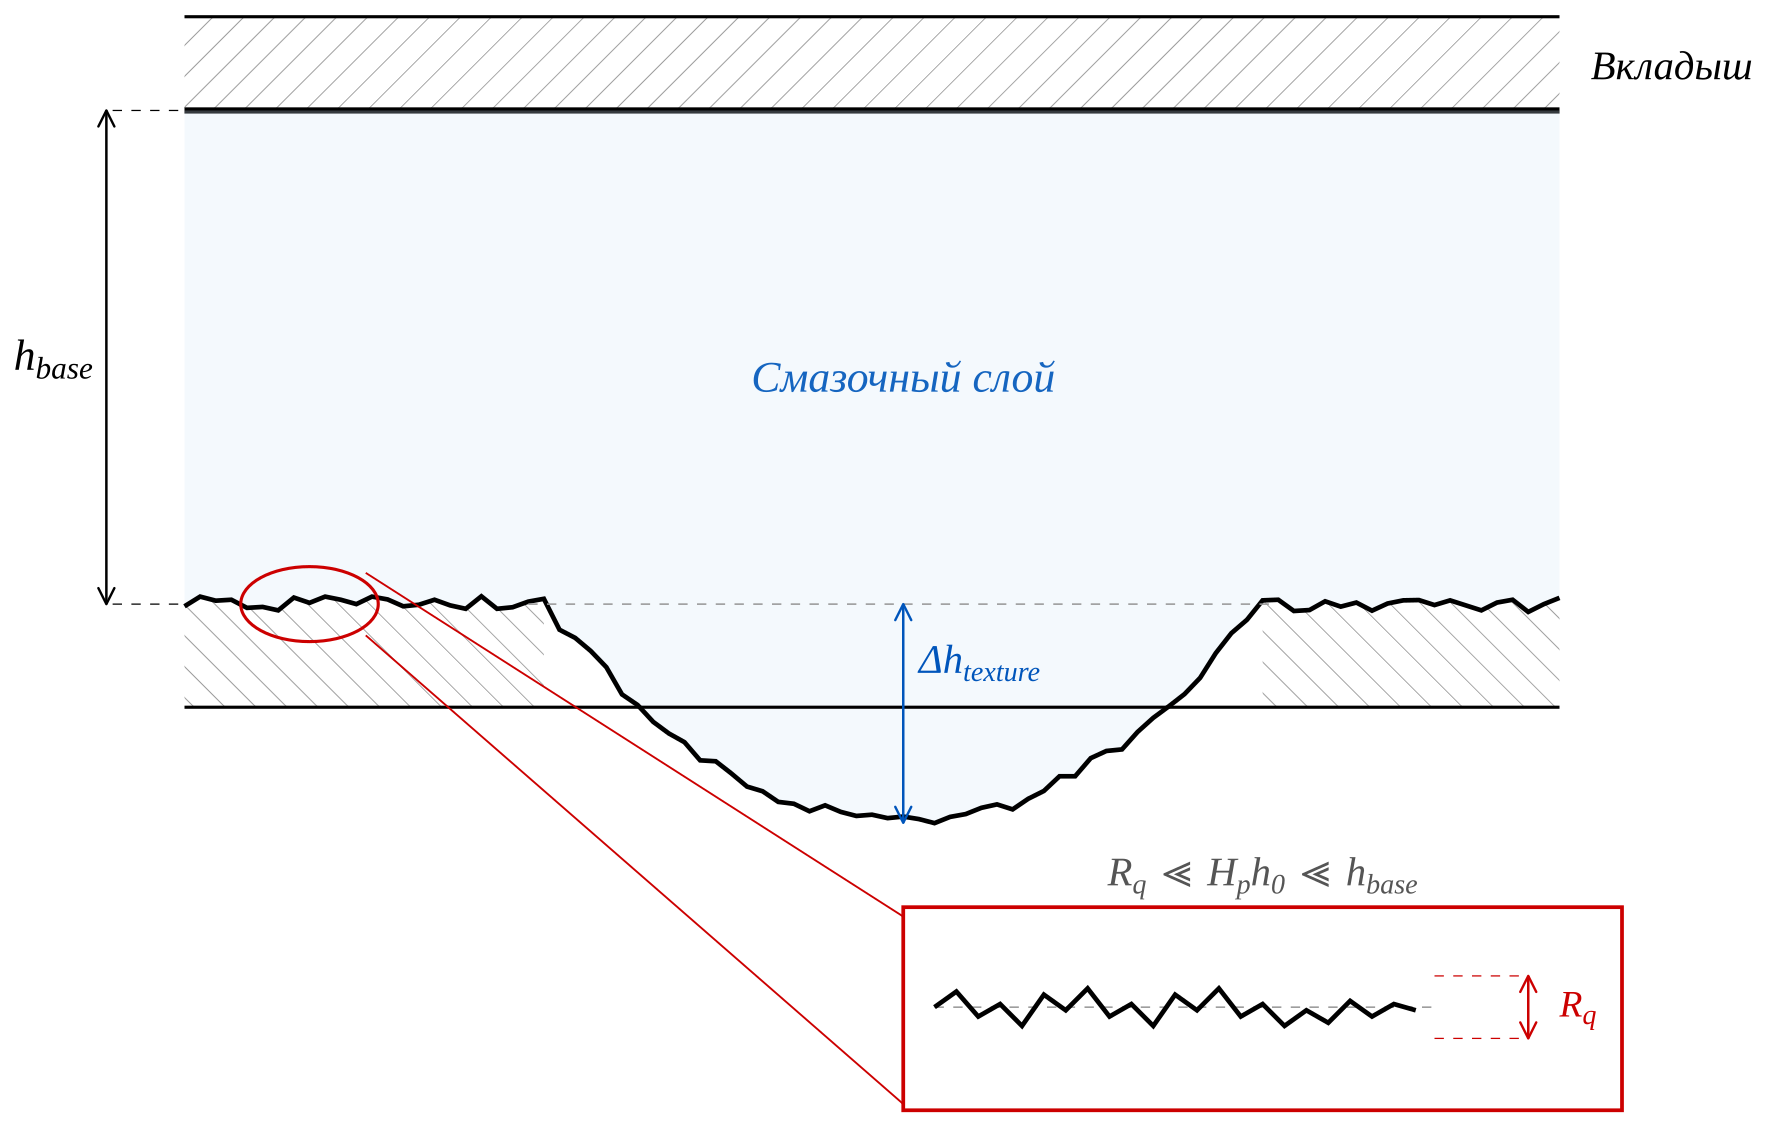
\includegraphics[width=\textwidth,height=0.9\textheight,keepaspectratio]{figures/ch04/fig_4_4.png}
\caption{Иерархия масштабов топографии поверхности:
  базовый зазор, детерминированная микротекстура и шероховатость}
\label{fig:roughness_scales}
\end{figure}

\FloatBarrier

\textit{Подходы к учёту шероховатости в уравнении Рейнольдса.}
В литературе сложились три основных подхода, различающихся
по сложности реализации и области применимости.

Первый подход~-- детерминированный: шероховатость задаётся явным
полем $\Delta h_{\mathrm{rough}}(s_1, s_2)$, полученным по данным
измерений (атомно-силовая микроскопия, контактная профилометрия),
и добавляется в суперпозицию зазора наряду с текстурой:
\[
  h = h_{\mathrm{base}} + \Delta h_{\mathrm{texture}}
    + \Delta h_{\mathrm{rough}}.
\]
Такой подход требует измеренного профиля поверхности
и разрешения расчётной сетки, достаточного для представления
случайного рельефа: шаг сетки должен быть существенно меньше
длины корреляции~$\lambda_c$ (единицы микрометров). Это приводит
к значительному увеличению числа узлов по сравнению с задачей для
гладких поверхностей (глава~3) и обоснованно только в рамках
исследовательских расчётов.

Второй подход~-- стохастический, основанный на осреднении
уравнения Рейнольдса по ансамблю реализаций случайной
шероховатости. Пионерская модель Кристенсена (Christensen, 1969)
и её развитие в работах Патира и Ченга (Patir, Cheng, 1978--1979)
вводят поправочные коэффициенты (\textit{flow factors}), которые
учитывают влияние статистической шероховатости на средние потоки
смазки. Осреднённое уравнение Рейнольдса записывается для
среднего давления~$\bar{p}$ с модифицированными коэффициентами:
\begin{equation}
  \frac{\partial}{\partial s_1}\!\left(\phi_p\,\bar{h}^3\,
  \frac{\partial \bar{p}}{\partial s_1}\right)
  + \Lambda^2\frac{\partial}{\partial s_2}\!\left(\phi_p\,\bar{h}^3\,
  \frac{\partial \bar{p}}{\partial s_2}\right)
  = \phi_s\,\frac{\partial \bar{h}}{\partial s_1}
  + \phi_c\,\sigma_r\,\frac{\partial \phi_s}{\partial s_1}\,,
  \label{eq:reynolds_rough_avg}
\end{equation}
\begin{conditions}
$\bar{h}$ -- номинальная (без случайной составляющей) толщина зазора: $\bar{h} = h_{\mathrm{base}} + \Delta h_{\mathrm{texture}}$ (суперпозиция~\eqref{eq:h_superposition} без~$\Delta h_{\mathrm{rough}}$);\\
$\bar{p}$ -- осреднённое давление;\\
$\phi_p$ -- фактор давления (pressure flow factor),
корректирующий пуазейлевский поток;\\
$\phi_s$ -- фактор сдвига (shear flow factor),
корректирующий куэттовский поток;\\
$\phi_c$ -- контактный фактор;\\
$\sigma_r$ -- суммарная среднеквадратичная шероховатость
контактирующих поверхностей, м ($\sigma_r \equiv R_q$ из~\eqref{eq:lambda_roughness});\\
$\Lambda$ -- отношение масштабов длины
(подраздел~2.1.6).
\end{conditions}
Факторы~$\phi_p$, $\phi_s$ зависят от отношения~$\bar{h}/\sigma_r$
и от ориентации шероховатости (продольная, поперечная,
изотропная). Они вычисляются однократно по статистическим
параметрам поверхности и не требуют разрешения случайного поля
на расчётной сетке, что делает стохастический подход
вычислительно эффективным. Структура
уравнения~\eqref{eq:reynolds_rough_avg} сохраняет форму исходного
уравнения Рейнольдса~\eqref{eq:reynolds_full}, поэтому солверы
и алгоритмы, описанные в главе~3, могут быть адаптированы
с минимальными изменениями. Член с~$\phi_c$ представляет дополнительную поправку, связанную с контактными эффектами при малых значениях~$\lambda_r$; в чисто гидродинамическом режиме ($\lambda_r > 5$) он мал и может быть опущен.

Третий подход~-- пренебрежение шероховатостью: при $\lambda_r \gg 1$
полагается $\Delta h_{\mathrm{rough}} = 0$, и уравнение Рейнольдса
решается для номинального зазора~\eqref{eq:h_superposition}. Это
допущение принято в расчётах глав~5--7 настоящей монографии.

\textit{Взаимодействие шероховатости с детерминированными
микроструктурами.}
При совместном присутствии детерминированных микроструктур
и случайной шероховатости характерные масштабы могут различаться
на порядки. Глубина ячейки микрорельефа~$h_p = H_p \cdot h_0$
составляет, как правило, единицы микрометров (в зависимости от технологии и назначения подшипника) при характерном размере
ячейки в десятки микрометров; шероховатость полированных
поверхностей характеризуется значениями $R_q \sim 0{,}01\text{--}0{,}1$~мкм
при длине корреляции $\lambda_c \sim 1\text{--}10$~мкм.

Когда $R_q \ll H_p \cdot h_0$~-- типичный случай при хорошо
обработанных поверхностях~-- детерминированные микроструктуры
доминируют в формировании поля давления и потоков, а вклад
шероховатости сводится к слабому стохастическому возмущению,
не влияющему на интегральные характеристики подшипника.

Когда $R_q$ оказывается соизмерима с~$H_p \cdot h_0$, что
возможно при грубой обработке или мелком микрорельефе,
шероховатость модифицирует распределение давления внутри ячеек
текстуры, изменяет локальные кавитационные зоны
(раздел~4.1) и может как усилить, так и ослабить эффективность
текстурирования. В этом режиме результаты, полученные в рамках
модели гладких поверхностей, требуют поправок, и корректное
описание предполагает использование одного из рассмотренных выше
подходов~-- детерминированного или стохастического.

Практический вывод для проектирования состоит в том, что
глубина детерминированных микроструктур~$h_p$ должна существенно
превышать среднеквадратичную шероховатость ($H_p \cdot h_0 \gg R_q$),
чтобы регулярный рельеф не терял функциональности на фоне случайных
микронеровностей. Это условие одновременно обеспечивает
$\lambda_r \gg 1$, при котором пренебрежение шероховатостью
в уравнении Рейнольдса обосновано.

В расчётах глав~5--7 поверхности приняты гладкими:
$\Delta h_{\mathrm{rough}} = 0$. Допущение оправдано при
$\lambda_r \gg 1$ и $H_p \cdot h_0 \gg R_q$, что типично
для прецизионных подшипников с полированными поверхностями.
Стохастический подход с коэффициентами потоков~$\phi_p$,
$\phi_s$~\eqref{eq:reynolds_rough_avg} представляет наиболее
практичный путь расширения модели на случай существенной
шероховатости: он сохраняет структуру дискретизации и не требует
разрешения случайного поля на расчётной сетке.
Детерминированный подход применим при наличии измеренных профилей
поверхности и вычислительных ресурсов для высокого разрешения
сетки, характерного масштаба $\lambda_c$.
При необходимости кавитация учитывается постановкой JFO для осреднённого давления~$\bar{p}$, т.\,е.\ условия комплементарности~\eqref{eq:jfo_complementarity} применяются к уравнению~\eqref{eq:reynolds_rough_avg}~\cite{gu2017,nie2022}.

\textit{Физический смысл коэффициентов потока Патира--Ченга.}
В модели Патира--Ченга~\cite{patir1978} исходное уравнение
Рейнольдса заменяется осреднённым уравнением с коэффициентами
потока $\phi_x$, $\phi_y$ (по давлению) и $\phi_s$ (по сдвигу):
%
\begin{equation}
  \frac{\partial}{\partial x}\!\left[\phi_x\,\bar{h}^3\,
  \frac{\partial \bar{p}}{\partial x}\right]
  + \frac{\partial}{\partial y}\!\left[\phi_y\,\bar{h}^3\,
  \frac{\partial \bar{p}}{\partial y}\right]
  = 6\mu U\,\frac{\partial}{\partial x}\!\left(\bar{h}
  + \phi_s\,\sigma_{\mathrm{eq}}\right).
  \label{eq:patir_cheng}
\end{equation}
%
Коэффициент $\phi_s$ описывает дополнительный перенос смазки
за счёт шероховатости (неоднородности переносного потока),
а $\phi_x$, $\phi_y$ отражают анизотропное сопротивление
шероховатости напорному потоку. Все три коэффициента зависят
от параметра $\lambda_r = \bar{h}/\sigma_{\mathrm{eq}}$
и ориентации шероховатости (изотропная, продольная,
поперечная). При $\lambda_r \gg 1$ все коэффициенты стремятся
к единице и уравнение~\eqref{eq:patir_cheng} вырождается
в классическое уравнение Рейнольдса.
При $\lambda_r < 3$ поправки становятся существенными:
$\phi_x$ и $\phi_y$ снижаются ниже единицы (шероховатость
затрудняет напорное течение), тогда как $\phi_s$ может
превышать единицу или быть меньше в зависимости от ориентации.

\textit{Обоснование допущения о гладких поверхностях.}
Допущение о гладких поверхностях ($\phi_x = \phi_y = 1$,
$\phi_s = 0$) принято в прикладных расчётах настоящей работы.
Его обоснование: параметр
$\lambda_r = h_{\min}/\sigma_{\mathrm{eq}}$ в характерных
режимах составляет $\lambda_r \geq 2$ (смешанный режим),
при котором поправки Патира--Ченга имеют ограниченное влияние
на интегральные характеристики и слабо меняют сравнительный
вывод о преимуществе текстурированного варианта над гладким.
Кроме того, детерминированная текстура (глубина
$H_p = 0{,}2$--$0{,}4$ в единицах зазора) по амплитуде
существенно превосходит стохастическую шероховатость
(характерная высота
$\sigma_{\mathrm{eq}} \ll h_{\min}$), поэтому вклад
случайного микрорельефа в интегральные характеристики
подшипника значительно меньше вклада детерминированных лунок.
Включение модели Патира--Ченга потребовало бы ввода
дополнительных параметров (тип и ориентация шероховатости,
коэффициенты потока), которые выходят за рамки исследуемых
переменных, не изменяя качественных выводов работы.


% \FloatBarrier
% \section{Динамика смазочного слоя}
% % sec_4_4_dynamics.tex — Динамика смазочного слоя

Разделы~4.1--4.3 рассматривали нелинейные эффекты применительно к~стационарному вращению вала при~фиксированном положении его~центра. В~реальных условиях эксплуатации вал совершает малые колебания относительно равновесного положения под~действием дисбаланса, переходных нагрузок и~гидродинамических возмущений. Реакция смазочного слоя на~эти~колебания описывается линеаризованными коэффициентами жёсткости и~демпфирования, которые определяют динамические свойства опорного узла и~устойчивость роторной системы в~целом~\cite{goodwin1997,jang1999,sayed2022,muszynska1988,weissbacher2014}.

\textit{Линеаризация по~малым возмущениям положения вала.}
Равновесное положение центра вала характеризуется координатами~$(x_0,\,y_0)$ или, эквивалентно, эксцентриситетом~$\varepsilon_0$ и~углом нагружения~$\psi_0$. При~малом возмущении центр вала смещается в~положение~$(x_0 + \xi,\; y_0 + \eta)$, где~$|\xi|,\,|\eta| \ll c$.

Безразмерная толщина зазора с~учётом возмущения записывается в~виде
\begin{equation}
  H(\theta,\,t) = H_0(\theta)
    - \bar{\xi}(t)\,\cos\theta
    - \bar{\eta}(t)\,\sin\theta,
  \label{eq:H_perturbed}
\end{equation}
\begin{conditions}
$H_0(\theta) = 1 + \varepsilon_0\cos\theta$ -- равновесный зазор радиального подшипника~\eqref{eq:journal_h};\\
$\bar{\xi} = \xi/c$,\; $\bar{\eta} = \eta/c$ -- безразмерные составляющие возмущения положения центра вала.
\end{conditions}
Давление разлагается по~малому параметру:
\begin{equation}
  P = P_0
    + \bar{\xi}\,P_{\xi}
    + \bar{\eta}\,P_{\eta}
    + \dot{\bar{\xi}}\,P_{\dot\xi}
    + \dot{\bar{\eta}}\,P_{\dot\eta}
    + \ldots
  \label{eq:P_expansion}
\end{equation}
Здесь~$P_0$~-- стационарное давление (главы~5--7); поля~$P_{\xi}$, $P_{\eta}$, $P_{\dot\xi}$, $P_{\dot\eta}$ находятся из~линеаризованных уравнений Рейнольдса с~правыми частями, получаемыми дифференцированием~\eqref{eq:reynolds_nondim} по~соответствующим переменным.

В~постановке JFO~\eqref{eq:jfo_conservation} граница кавитационной области при~возмущении может смещаться. В~первом приближении используется допущение о~фиксированной кавитационной области (\textit{frozen cavitation}): граница~$\partial\Omega_{\mathrm{cav}}$ определяется по~равновесному полю~$P_0$. Альтернативные подходы и~их~сравнение рассматриваются в~главе~8.

\textit{Матрицы жёсткости и~демпфирования смазочного слоя.}
Линеаризация гидродинамической силы приводит к~выражению
\begin{equation}
  \begin{pmatrix} \Delta F_x \\ \Delta F_y \end{pmatrix}
  = -\mathbf{K}
  \begin{pmatrix} \bar\xi \\ \bar\eta \end{pmatrix}
  - \mathbf{C}
  \begin{pmatrix} \dot{\bar\xi} \\ \dot{\bar\eta} \end{pmatrix},
  \label{eq:linearized_force}
\end{equation}
где~компоненты матриц жёсткости~$\mathbf{K}$ и~демпфирования~$\mathbf{C}$ определяются как
\begin{equation}
  K_{ij} = -\frac{\partial F_i}{\partial \bar{q}_j}\bigg|_0, \qquad
  C_{ij} = -\frac{\partial F_i}{\partial \dot{\bar{q}}_j}\bigg|_0,
  \quad i,j \in \{x,\,y\},
  \label{eq:KC_def}
\end{equation}
а~численное вычисление выполняется интегрированием возмущённых давлений по~области смазочного слоя:
\begin{equation}
  K_{xx} = -\iint_\Omega P_{\xi}\,\cos\theta\;d\theta\,dZ, \qquad
  K_{xy} = -\iint_\Omega P_{\eta}\,\cos\theta\;d\theta\,dZ,
  \label{eq:K_integrals}
\end{equation}
аналогично для~$K_{yx}$, $K_{yy}$ и~для~$C_{xx}$, $C_{xy}$, $C_{yx}$, $C_{yy}$ через~$P_{\dot\xi}$, $P_{\dot\eta}$.

Детерминированные микроструктуры изменяют стационарное поле~$P_0$ и~возмущённые поля~$P_{\xi}$, $P_{\eta}$, $P_{\dot\xi}$, $P_{\dot\eta}$, а~следовательно, компоненты~$K_{ij}$ и~$C_{ij}$. Это~является основным каналом влияния текстуры поверхности на~динамические характеристики опорного узла. Матрицы~$\mathbf{K}$ и~$\mathbf{C}$ в~общем случае несимметричны: перекрёстные коэффициенты~$K_{xy} \neq K_{yx}$, $C_{xy} \neq C_{yx}$, что~обусловлено вращательным характером течения смазки и~является принципиальным отличием подшипников скольжения от~упругих опор.

\textit{Критерии устойчивости роторно-подшипниковой системы.}
Уравнение движения ротора массой~$M$ в~двухкоординатной ($2$DOF) модели записывается в~виде
\begin{equation}
  M\,\ddot{\mathbf{q}} + \mathbf{C}\,\dot{\mathbf{q}} + \mathbf{K}\,\mathbf{q} = 0,
  \qquad \mathbf{q} = (\bar\xi,\,\bar\eta)^T.
  \label{eq:rotor_eom}
\end{equation}
Переход к~переменным состояния~$\mathbf{u} = (\mathbf{q},\,\dot{\mathbf{q}})^T$ приводит систему к~стандартной форме
\begin{equation}
  \dot{\mathbf{u}} = \mathbf{A}\,\mathbf{u}, \qquad
  \mathbf{A} =
  \begin{pmatrix}
    \mathbf{0} & \mathbf{I} \\
    -M^{-1}\mathbf{K} & -M^{-1}\mathbf{C}
  \end{pmatrix}.
  \label{eq:state_matrix}
\end{equation}
Система асимптотически устойчива тогда и~только тогда, когда все~собственные значения~$\lambda_k$ матрицы~$\mathbf{A}$ имеют отрицательную вещественную часть: $\mathrm{Re}(\lambda_k) < 0$ для~всех~$k$. Если~хотя~бы~для~одного~$k$ выполняется~$\mathrm{Re}(\lambda_k) > 0$, система неустойчива; граничный случай~$\max_k \mathrm{Re}(\lambda_k) = 0$ соответствует порогу устойчивости (критической скорости).

Формулы для~критических скоростей и~интегральных критериев устойчивости зависят от~конкретной модели ротора (масса, жёсткость вала, гироскопика) и~в~данном разделе не~приводятся; количественный пример применительно к~подшипнику центробежного насоса рассматривается в~главе~8.

Общая схема линеаризованной модели сил смазочного слоя
приведена на рисунке~\ref{fig:linearized_forces}.

\begin{figure}[!ht]
\centering
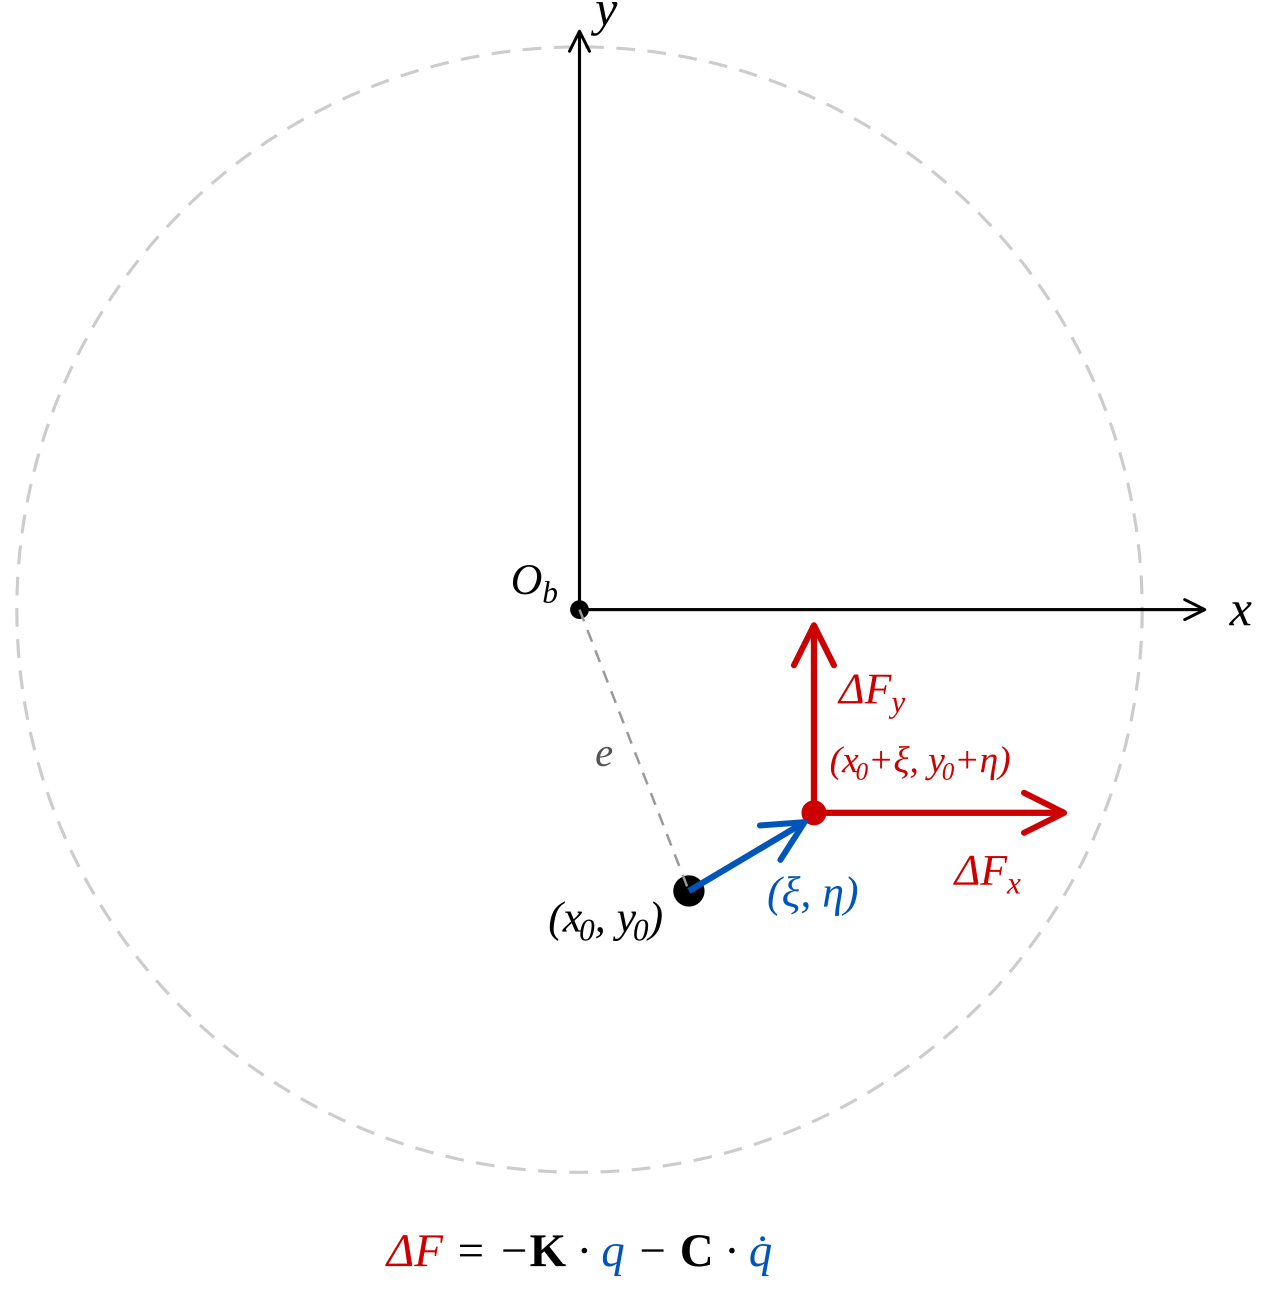
\includegraphics[width=\textwidth,height=0.9\textheight,keepaspectratio]{figures/ch04/fig_4_5.png}
\caption{Линеаризованная модель сил смазочного слоя при малых колебаниях вала}
\label{fig:linearized_forces}
\end{figure}

\FloatBarrier

Линеаризованные коэффициенты жёсткости и~демпфирования
полностью определяются стационарным и~возмущёнными полями
давления; влияние детерминированных микроструктур на~эти
коэффициенты и~устойчивость роторной системы количественно
исследуется в~главе~8.

\textit{Физический смысл прямых и перекрёстных коэффициентов.}
Физический смысл коэффициентов целесообразно пояснить
на примере радиального подшипника. Прямые
жёсткости $K_{xx}$, $K_{yy}$ характеризуют возвращающую силу
при смещении вала вдоль соответствующей оси: $K_{xx} > 0$
означает, что смещение по~$x$ порождает силу, направленную
против смещения (упругоподобное поведение). Прямые
демпфирования $C_{xx}$, $C_{yy}$ определяют диссипативные
силы, противодействующие скорости вала: $C_{xx} > 0$ означает
торможение при движении по~$x$.

Перекрёстные коэффициенты~$K_{xy}$, $K_{yx}$, $C_{xy}$,
$C_{yx}$ описывают связь между двумя направлениями движения.
Для подшипника скольжения перекрёстные жёсткости обычно имеют
противоположные знаки: $K_{xy} > 0$, $K_{yx} < 0$. Это
соответствует циркуляторным силам~-- силам, перпендикулярным
скорости; они не совершают работы в среднем за период,
но могут раскачивать орбиту. Именно наличие циркуляторной пары
$K_{xy} \neq 0$, $K_{yx} \neq 0$ является физическим
механизмом нестабильности типа «вихревая прецессия»
(oil whirl), характерной для подшипников скольжения при
больших скоростях.

\textit{Механизм нестабильности типа вихревой прецессии и~роль текстуры.}
Нестабильность типа oil whirl (вихревая прецессия) возникает, когда циркуляторные силы от~перекрёстных жёсткостей превышают диссипацию от~прямых демпфирований. В~линейной модели~\eqref{eq:rotor_eom} критерий потери устойчивости формулируется через знак~$\mathrm{Re}(\lambda)$, однако физически механизм можно описать следующим образом. При~смещении центра вала по~направлению~$x$ возникает сила~$K_{yx}\,\xi$ в~направлении~$y$ (при~$K_{yx} < 0$ --- это сила, перпендикулярная смещению и~направленная по~вращению). Эта сила раскручивает орбиту вала, постепенно увеличивая её~радиус. Прямое демпфирование~$C_{xx}$, $C_{yy}$ противодействует этому процессу, но~при~достаточно высоких скоростях вращения (и~соответственно высоком давлении смазки) циркуляторная сила превышает диссипацию, и~орбита начинает раскручиваться неограниченно~--- наступает нестабильность.

Детерминированные микроструктуры влияют на~этот баланс через~два канала. С~одной стороны, они изменяют равновесное поле давления~$P_0$ и~тем самым модифицируют все~восемь коэффициентов. С~другой стороны, они изменяют геометрию зазора~$H$, что непосредственно сказывается на~возмущённых полях~$P_\xi$, $P_\eta$, $P_{\dot\xi}$, $P_{\dot\eta}$. Результирующий эффект определяется расположением и~геометрией лунок: текстура во~входной части клина может усиливать прямые жёсткости и~улучшать демпфирование, тогда как~текстура в~зоне убывающего давления оказывает обратное действие~--- это качественно согласуется с~результатами глав~5--7 по~статическому анализу.

\textit{Ограниченность линейной модели.}
Линейная модель~\eqref{eq:rotor_eom} применима только при~малых амплитудах колебаний~$|\xi|, |\eta| \ll c$. При~амплитудах, сопоставимых с~зазором~$c$, нелинейные эффекты становятся существенными: форма орбиты отклоняется от~эллиптической, спектр колебаний обогащается гармониками, а~в~некоторых случаях возникают квазипериодические или хаотические режимы движения. В~этих условиях применение линейных коэффициентов~$K_{ij}$, $C_{ij}$ приводит к~качественно неверным предсказаниям. Полноценный нелинейный анализ требует численного интегрирования уравнений движения с~пересчётом поля давления на~каждом временном шаге, что в~несколько порядков увеличивает вычислительные затраты. Для~целей данной монографии рассматривается только линейная модель; проверка её~применимости выполняется через сравнение максимальных амплитуд с~зазором~$c$ (глава~8).

\textit{Механизм нестабильности типа вихревой прецессии и~роль текстуры.}
Нестабильность типа oil whirl (вихревая прецессия) возникает, когда циркуляторные силы от~перекрёстных жёсткостей превышают диссипацию от~прямых демпфирований. В~линейной модели~\eqref{eq:rotor_eom} критерий потери устойчивости формулируется через знак~$\mathrm{Re}(\lambda)$, однако физически механизм можно описать следующим образом. При~смещении центра вала по~направлению~$x$ возникает сила~$K_{yx}\,\xi$ в~направлении~$y$ (при~$K_{yx} < 0$~--- это сила, перпендикулярная смещению и~направленная по~вращению). Эта сила раскручивает орбиту вала, постепенно увеличивая её~радиус. Прямое демпфирование~$C_{xx}$, $C_{yy}$ противодействует этому процессу, но~при~достаточно высоких скоростях вращения (и~соответственно высоком давлении смазки) циркуляторная сила превышает диссипацию, и~орбита начинает раскручиваться неограниченно~--- наступает нестабильность.

Детерминированные микроструктуры влияют на~этот баланс через~два канала. С~одной стороны, они изменяют равновесное поле давления~$P_0$ и~тем самым модифицируют все~восемь коэффициентов. С~другой стороны, они изменяют геометрию зазора~$H$, что непосредственно сказывается на~возмущённых полях~$P_\xi$, $P_\eta$, $P_{\dot\xi}$, $P_{\dot\eta}$. Результирующий эффект определяется расположением и~геометрией лунок: текстура во~входной части клина может усиливать прямые жёсткости и~улучшать демпфирование, тогда как~текстура в~зоне убывающего давления оказывает обратное действие~--- это качественно согласуется с~результатами глав~5--7 по~статическому анализу.

\textit{Ограниченность линейной модели.}
Линейная модель~\eqref{eq:rotor_eom} применима только при~малых амплитудах колебаний~$|\xi|, |\eta| \ll c$. При~амплитудах, сопоставимых с~зазором~$c$, нелинейные эффекты становятся существенными: форма орбиты отклоняется от~эллиптической, спектр колебаний обогащается гармониками, а~в~некоторых случаях возникают квазипериодические или хаотические режимы движения. В~этих условиях применение линейных коэффициентов~$K_{ij}$, $C_{ij}$ приводит к~качественно неверным предсказаниям. Полноценный нелинейный анализ требует численного интегрирования уравнений движения с~пересчётом поля давления на~каждом временном шаге, что в~несколько порядков увеличивает вычислительные затраты. Для~целей данной монографии рассматривается только линейная модель; проверка её~применимости выполняется через сравнение максимальных амплитуд с~зазором~$c$ (глава~8).

\textit{Связь с главой~8 и метод численного вычисления
коэффициентов.}
Аналитическое вычисление коэффициентов~$K_{ij}$, $C_{ij}$
через интегралы~\eqref{eq:K_integrals} требует решения
четырёх вспомогательных линеаризованных уравнений Рейнольдса.
Альтернативный численный подход, используемый в главе~8,
основан на методе центральных конечных разностей:
коэффициент $K_{xx}$ вычисляется как
$K_{xx} \approx -[F_x(x_0 + \Delta x) -
F_x(x_0 - \Delta x)]/(2\Delta x)$, где $F_x$ получается
прямым решением стационарного уравнения Рейнольдса при
возмущённом зазоре. Аналогично для коэффициентов демпфирования
решается динамическое уравнение Рейнольдса с ненулевой
скоростью возмущения~$\dot{x}$ или~$\dot{y}$. Точность
такого подхода определяется величиной шага конечных
разностей~$\Delta x$, $\Delta v$: при слишком большом шаге
нарушается линейное приближение, при слишком малом~-- результат
искажается численным шумом; оптимальный диапазон обсуждается
в разделе~8.4.


\FloatBarrier
\section*{Контрольные вопросы}
\phantomsection\addcontentsline{toc}{section}{Контрольные вопросы}

\begin{enumerate}
\item Что~такое кавитация в~контексте смазочного слоя?
\item Что~такое число подшипника~$\Lambda$ и~как оно~связано с~нелинейностью?
\item Как~учитывается изменение плотности смазки?
\item Какие термовязкостные эффекты влияют на~работу подшипника?
\item Как~зависит вязкость масла от~температуры?
\item Что~такое модель Патира--Ченга для~учёта шероховатости?
\item Какое влияние оказывает шероховатость на~нагрузочную способность?
\item В~чём отличие стохастической и~детерминированной моделей шероховатости?
\item Какие уровни учёта температуры существуют при~моделировании смазочного слоя?
\item Что~такое число смазочного слоя~$\lambda_r$ и~как оно~определяет режим трения?
\end{enumerate}
       % Глава 4: Учёт эффектов
\chapter{Курсовое проектирование}

\section{Цели и задачи курсового проектирования}

Целью курсового проектирования является закрепление теоретических знаний, полученных при~изучении глав~1-4, и~освоение методики расчёта подшипников скольжения с~дискретным микрорельефом рабочей поверхности.

В~процессе выполнения курсовой работы студент должен:
\begin{itemize}
\item сформулировать расчётную задачу для~подшипника скольжения заданного типа;
\item записать математическую модель смазочного слоя на~основе уравнения Рейнольдса;
\item задать параметры микрорельефа (тип элементов, глубину, размеры, схему расположения);
\item выполнить расчёт характеристик гладкого подшипника;
\item выполнить расчёт характеристик подшипника с~микрорельефом;
\item провести сравнительный анализ результатов, сделать выводы об~эффективности текстурирования;
\item оформить результаты в~виде пояснительной записки.
\end{itemize}

В~результате выполнения работы студент приобретает навыки самостоятельного инженерного расчёта подшипниковых узлов, анализа и~интерпретации результатов моделирования, а~также оформления технической документации.


\section{Указания к выполнению курсовой работы}

Рекомендуемый алгоритм выполнения курсовой работы:

\begin{enumerate}
\item \textbf{Получение задания.} Выбрать вариант из~таблицы~\ref{tab:variants} (по~указанию преподавателя или~по~номеру в~списке группы). Записать исходные данные: тип подшипника, геометрические размеры, параметры смазки, режим работы, тип и~параметры микрорельефа.

\item \textbf{Формулировка математической модели.} На~основе материала глав~2-3 записать уравнение Рейнольдса для~заданного типа подшипника, граничные условия, условие кавитации. Определить функцию зазора для~гладкого и~текстурированного вариантов. Записать формулы для~вычисления интегральных характеристик (несущая способность, коэффициент трения, утечки).

\item \textbf{Расчёт гладкого подшипника.} Выполнить численный расчёт поля давления и~интегральных характеристик для~подшипника без~микрорельефа. Этот~расчёт является базовым (эталонным) для~последующего сравнения.

\item \textbf{Задание параметров микрорельефа.} В~соответствии с~вариантом задания определить геометрию элементов (глубину, размеры), схему расположения и~зону нанесения текстуры. Записать функцию добавки к~зазору~$\Delta h$.

\item \textbf{Расчёт текстурированного подшипника.} Выполнить численный расчёт с~учётом микрорельефа. Получить поля давления, кавитационные зоны и~интегральные характеристики.

\item \textbf{Сравнительный анализ.} Вычислить нормированные показатели эффективности (отношение характеристик текстурированного подшипника к~гладкому). Построить графики зависимостей. Проанализировать влияние параметров микрорельефа.

\item \textbf{Оформление пояснительной записки.} Оформить работу в~соответствии с~требованиями раздела~\ref{sec:requirements}.
\end{enumerate}


\section{Варианты курсовой работы}\label{sec:variants}

Варианты курсовой работы приведены в~таблице~\ref{tab:variants}. Каждый вариант определяет тип подшипника, основные размеры, режим работы, тип смазки и~параметры микрорельефа.

\begin{table}[!ht]
\centering
\caption{Варианты курсовой работы}
\label{tab:variants}
\small
\begin{tabularx}{\textwidth}{|c|X|c|c|c|c|c|}
\hline
\textbf{№} & \textbf{Тип подшипника} & $\boldsymbol{R}$, \textbf{мм} & $\boldsymbol{L}$, \textbf{мм} & $\boldsymbol{c}$, \textbf{мкм} & $\boldsymbol{n}$, \textbf{об/мин} & \textbf{Тип рельефа} \\
\hline
1  & Радиальный & 30 & 48 & 40 & 3000 & Лунки \\
\hline
2  & Радиальный & 35 & 56 & 50 & 2980 & Лунки \\
\hline
3  & Радиальный & 40 & 64 & 60 & 1500 & Лунки \\
\hline
4  & Радиальный & 25 & 40 & 35 & 6000 & Лунки \\
\hline
5  & Радиальный & 50 & 80 & 70 & 1000 & Канавки \\
\hline
6  & Радиальный & 30 & 40 & 60 & 120  & Лунки \\
\hline
7  & Радиальный & 35 & 50 & 45 & 4500 & Лунки \\
\hline
8  & Радиальный & 45 & 72 & 55 & 2000 & Канавки \\
\hline
9  & Радиальный & 30 & 48 & 40 & 3600 & Лунки \\
\hline
10 & Радиальный & 40 & 56 & 50 & 2500 & Лунки \\
\hline
11 & Упорный    & 30 & --  & 50 & 3000 & Лунки \\
\hline
12 & Упорный    & 40 & --  & 40 & 1500 & Лунки \\
\hline
13 & Упорный    & 50 & --  & 60 & 3600 & Канавки \\
\hline
14 & Упорный    & 35 & --  & 45 & 6000 & Лунки \\
\hline
15 & Упорный    & 25 & --  & 35 & 2000 & Лунки \\
\hline
\end{tabularx}
\end{table}

\FloatBarrier

\textit{Примечания к таблице~\ref{tab:variants}:}
\begin{itemize}
\item для~радиальных подшипников~$R$~-- радиус вала, $L$~-- длина подшипника, $c$~-- радиальный зазор;
\item для~упорных подшипников~$R$~-- внутренний радиус, наружный радиус $R_{\mathrm{out}} = 2R$, параметр клина $K = 2{,}0$, минимальный зазор~$h_{\mathrm{out}} = c$, число колодок~$N = 6$;
\item динамическая вязкость смазки для~всех вариантов $\mu = 0{,}01$~Па$\cdot$с (масло ISO~VG~32 при~$40\,^{\circ}$C), если иное не~указано преподавателем;
\item тип рельефа <<Лунки>>~-- эллипсоидальные лунки в~шахматной раскладке; <<Канавки>>~-- поперечные канавки параболического профиля;
\item безразмерная глубина элементов $H_p$, зона нанесения и~число элементов выбираются студентом самостоятельно на~основе рекомендаций, изложенных в~примерах данной главы.
\end{itemize}


\section{Требования к пояснительной записке и графическому материалу}\label{sec:requirements}

Пояснительная записка к~курсовой работе должна содержать следующие разделы:

\begin{enumerate}
\item Титульный лист (по~форме, установленной кафедрой).
\item Задание на~курсовую работу.
\item Содержание.
\item Введение: цель работы, краткое описание объекта исследования.
\item Исходные данные: параметры подшипника, смазки, микрорельефа (в~виде таблицы).
\item Математическая модель: уравнение Рейнольдса, граничные условия, функция зазора, интегральные функционалы.
\item Результаты расчёта гладкого подшипника: поля давления, интегральные характеристики, графики.
\item Результаты расчёта текстурированного подшипника: поля давления, интегральные характеристики, графики.
\item Сравнительный анализ: нормированные показатели эффективности, таблицы сравнения, графики.
\item Выводы: основные результаты, рекомендации.
\item Список использованных источников.
\end{enumerate}

\textbf{Объём} пояснительной записки~-- 25-40~страниц (без~приложений).

\textbf{Оформление}~-- в~соответствии с~СТУ~7.5-07-2021 СФУ: формат~A4, шрифт Times New Roman 14~пт, одинарный межстрочный интервал, поля: левое~-- 30~мм, правое~-- 10~мм, верхнее и~нижнее~-- 20~мм, абзацный отступ~-- 12,5~мм. Рисунки и~таблицы оформляются в~соответствии с~ГОСТ.

\textbf{Графический материал:}
\begin{itemize}
\item схема подшипника с~указанием основных размеров;
\item карта распределения зазора (для~текстурированного варианта);
\item поле давления для~гладкого и~текстурированного подшипников;
\item графики зависимостей интегральных характеристик;
\item диаграмма нормированных показателей эффективности.
\end{itemize}


\section{Пример анализа радиального подшипника скольжения центробежного насоса}

Ниже приведён подробный пример расчёта радиального подшипника скольжения ротора центробежного насоса. Пример демонстрирует полный цикл анализа: от~задания исходных данных через формулировку математической модели и~выполнение расчёта к~сравнению гладкого и~текстурированного вариантов и~формулированию выводов. Рекомендуется использовать данный пример как~образец при~выполнении курсовой работы для~радиального подшипника.

% =============================================================
% 5 Анализ радиального подшипника скольжения
%   центробежного насоса
% =============================================================
\chapter{Анализ рельефного радиального подшипника скольжения центробежного насоса}

\section{Объект исследования и исходные данные}

Объектом исследования в настоящей главе является радиальный
подшипник скольжения ротора центробежного насоса~\cite{bashmur2024a}.
Подшипниковый узел предназначен для восприятия радиальных
нагрузок, передаваемых от ротора к корпусу, и обеспечения
жидкостного режима смазки в рабочем диапазоне скоростей
и нагрузок.

Подшипник представляет собой цилиндрическую пару: вал
радиуса~$R$ вращается внутри вкладыша с радиальным зазором~$c$.
Относительный зазор $\psi = c/R$ определяет геометрическую
характеристику подшипника; отношение длины к диаметру~$L/D$
характеризует его осевую протяжённость. Рабочей средой является
масло с динамической вязкостью~$\mu_0$ при референсной
температуре~$T_0$. Вал вращается с угловой скоростью~$\omega$
и нагружен радиальной силой~$F_{\mathrm{ext}}$, действующей
в плоскости поперечного сечения.

Расчёт выполняется в изотермическом приближении: температура
смазки принята постоянной ($T = T_0$, $\mu = \mathrm{const}$),
что обосновано в разделе~4.2 при умеренных скоростях скольжения
и нагрузках, характерных для рассматриваемого узла. Плотность
смазки считается постоянной ($\rho = \mathrm{const}$),
поверхности~-- гладкими (обоснование~-- раздел~4.3).

Основные параметры подшипника сведены в таблицу~\ref{tab:journal_params}.

\begin{table}[!ht]
\centering
\caption{Параметры радиального подшипника скольжения}
\label{tab:journal_params}
\begin{tabularx}{\textwidth}{|X|c|c|c|}
\hline
\multicolumn{1}{|c|}{\textbf{Параметр}} & \textbf{Обозначение} & \textbf{Значение} & \textbf{Единица} \\
\hline
Радиус вала            & $R$              & 35{,}0  & мм \\
\hline
Длина подшипника       & $L$              & 56{,}0  & мм \\
\hline
Радиальный зазор       & $c$              & 50      & мкм \\
\hline
Относительный зазор    & $\psi = c/R$     & $1{,}43 \times 10^{-3}$ & -- \\
\hline
Отношение $L/D$        & $L/D$            & 0{,}80  & -- \\
\hline
Угловая скорость       & $\omega$         & 312{,}0 & рад/с \\
\hline
Динамическая вязкость  & $\mu_0$          & $1{,}105 \times 10^{-2}$ & Па$\cdot$с \\
\hline
Давление кавитации     & $p_{\mathrm{cav}}$ & 0     & Па \\
\hline
\end{tabularx}
\end{table}

\FloatBarrier

Схема подшипника в поперечном сечении представлена на
рисунке~\ref{fig:journal_scheme}.

\begin{figure}[!ht]
\centering
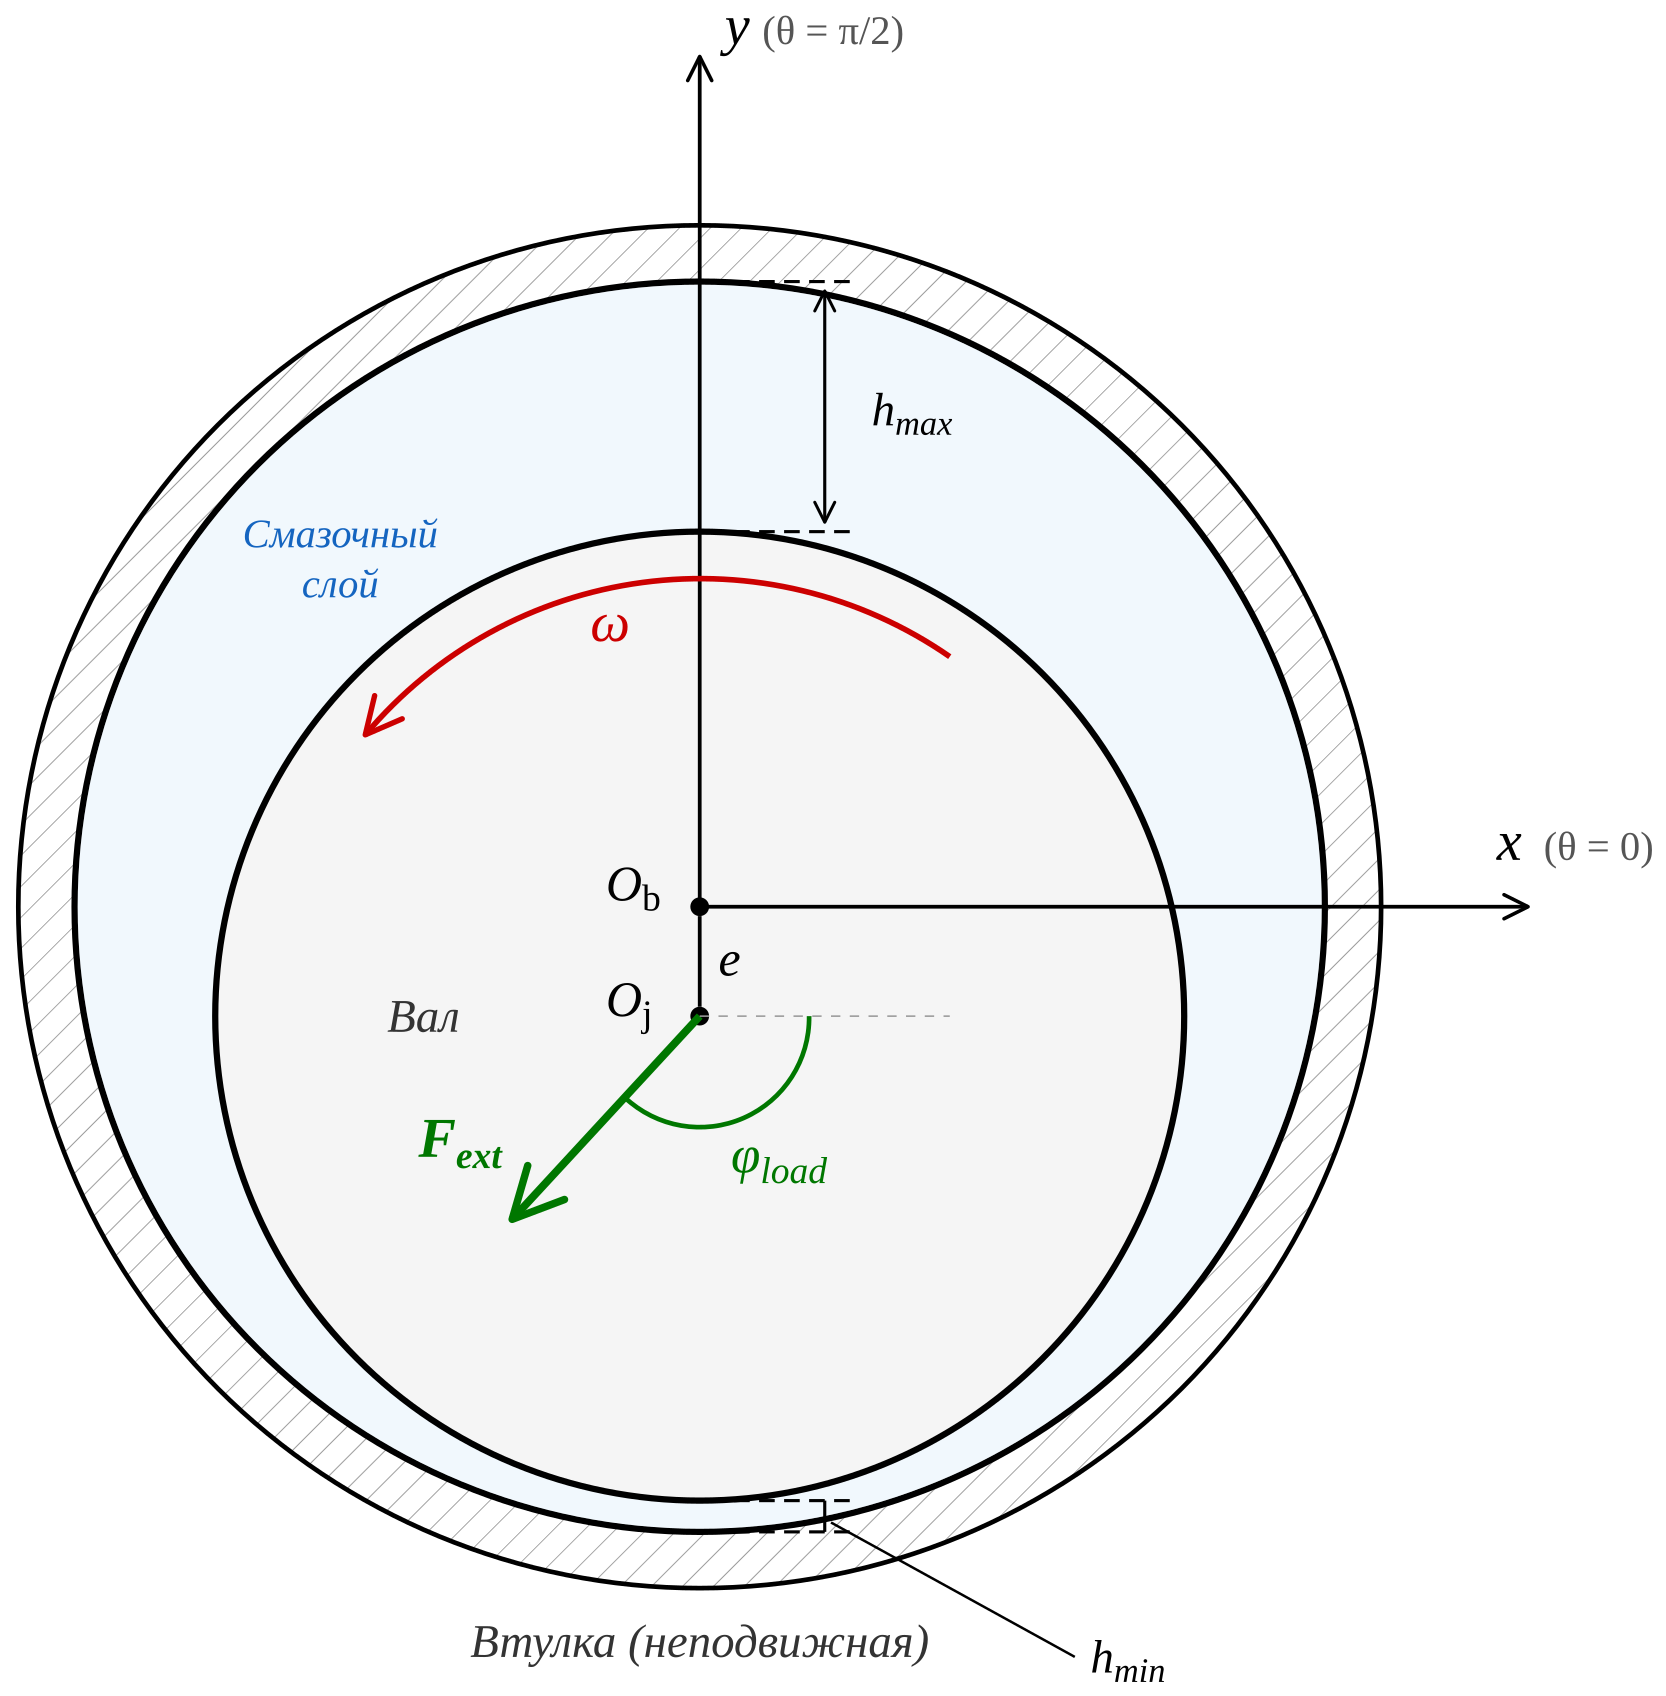
\includegraphics[width=\textwidth,height=0.9\textheight,keepaspectratio]{figures/ch05/fig_5_1.png}
\caption{Схема радиального подшипника скольжения центробежного насоса}
\label{fig:journal_scheme}
\end{figure}

\FloatBarrier

Обозначения на схеме соответствуют параметрам
таблицы~\ref{tab:journal_params}; направление отсчёта
угла~$\theta$ и положение начала координат определены
в разделе~\ref{sec:problem_statement_ch5}.

\section{Постановка задачи}\label{sec:problem_statement_ch5}

Расчётная область представляет собой развёрнутую поверхность
смазочного зазора $(\theta, z) \in [0,\,2\pi] \times [-L/2,\,L/2]$,
где $\theta$~-- окружная координата, $z$~-- осевая координата.
При переходе к безразмерным переменным (подраздел~2.1.6)
осевая координата нормируется на полудлину: $Z = 2z/L$,
так что $Z \in [-1,\,1]$.

В тексте главы окружная координата обозначается~$\theta$;
на рисунках ось подписана~$\varphi$; везде $\theta \equiv \varphi$.

Для гладкого цилиндрического подшипника безразмерная толщина
зазора определяется законом~\eqref{eq:journal_h}:
\begin{equation}
  H(\theta) = 1 + \varepsilon\cos\theta,
  \label{eq:journal_h_ch5}
\end{equation}
где $\varepsilon = e/c$~-- относительный эксцентриситет
($0 \leq \varepsilon < 1$), $e$~-- смещение оси вала
относительно оси вкладыша. При $\varepsilon = 0$ зазор
равномерный, при $\varepsilon \to 1$ минимальный зазор
$h_{\min} = c\,(1 - \varepsilon)$ стремится к нулю.

Для подшипника с детерминированными микроструктурами толщина
зазора записывается в виде суперпозиции~\eqref{eq:h_superposition}:
\begin{equation}
  H = H_{\mathrm{base}}(\theta) + \Delta H_{\mathrm{texture}}(\theta, Z),
  \label{eq:journal_h_tex_ch5}
\end{equation}
где $H_{\mathrm{base}} = 1 + \varepsilon\cos\theta$~-- базовый зазор
гладкого подшипника, $\Delta H_{\mathrm{texture}}$~-- добавка,
описывающая микрорельеф (подраздел~2.2, формула~\eqref{eq:journal_h_textured}).

Распределение давления в смазочном слое описывается безразмерным
уравнением Рейнольдса~\eqref{eq:reynolds_nondim} с параметром
анизотропии~$\Lambda$~\eqref{eq:nondim_Lambda}. Для радиального
подшипника $\Lambda = 2R/L$; данный параметр определяет
соотношение окружного и осевого масштабов задачи.

Кавитация учитывается по условию Рейнольдса: давление не допускается
ниже давления кавитации, т.е.\ $P \geq 0$; в области разрыва плёнки
принимается $P = 0$. Данное условие является упрощением постановки JFO
(\eqref{eq:jfo_conservation}, \eqref{eq:jfo_complementarity});
полная JFO-постановка составляет предмет дальнейшего развития модели.

Граничные условия задачи формулируются следующим образом:
по окружной координате~$\theta$ поле давления периодично
($P(\theta = 0) = P(\theta = 2\pi)$); на торцах подшипника
давление равно атмосферному ($P = 0$ при $Z = \pm 1$).

Допущения, принятые в настоящей главе, включают: изотермическое
приближение ($T = T_0$, обоснование~-- раздел~4.2), постоянство
плотности ($\rho = \mathrm{const}$, раздел~4.1) и гладкость
поверхностей ($\Delta h_{\mathrm{rough}} = 0$, раздел~4.3).

Расчётная область с граничными условиями схематически показана
на рисунке~\ref{fig:journal_domain}.

\begin{figure}[!ht]
\centering
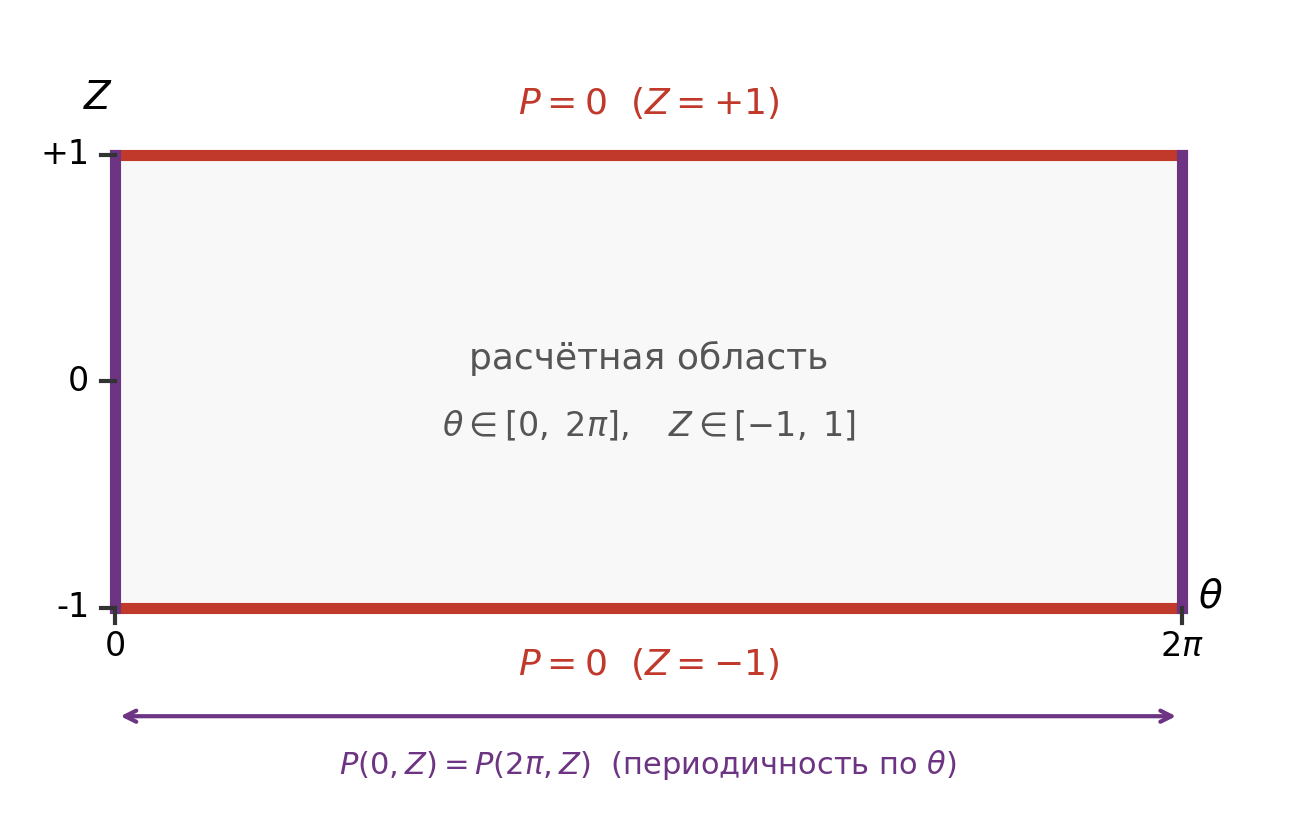
\includegraphics[width=\textwidth,height=0.9\textheight,keepaspectratio]{figures/ch05/fig_5_2.png}
\caption{Расчётная область $(\theta, Z) \in [0,\,2\pi] \times [-1,\,1]$
  и граничные условия: периодичность по~$\theta$, $P = 0$ на торцах
  $Z = \pm 1$; зона давления ($P > 0$) и кавитационная зона ($P = 0$)
  разделены границей кавитации (штриховая линия).}
\label{fig:journal_domain}
\end{figure}


\section{Результаты для гладкого подшипника}

Результаты расчёта гладкого подшипника (без микроструктур)
составляют эталонную базу для последующего сравнения
с текстурированным вариантом.

\textit{Поле давления и кавитация.}
При стационарном вращении вала под нагрузкой ось вала смещается
на величину эксцентриситета~$e$ относительно оси вкладыша.
В сходящейся части зазора ($0 < \theta < \pi$ при выбранной
системе координат) смазка увлекается в область с уменьшающимся
зазором, что формирует зону повышенного давления. В расходящейся
части ($\pi < \theta < 2\pi$) зазор увеличивается; при
отсутствии кавитации давление здесь становилось бы отрицательным
(ниже давления насыщения). Условие кавитации Рейнольдса ($P \geq 0$)
обнуляет давление в области, где оно падает ниже давления
кавитации, формируя кавитационную зону, в которой $P = 0$.
Распределение давления по окружной и осевой координатам, а также
расположение кавитационной зоны показаны на
рисунках~\ref{fig:smooth_P3D} и~\ref{fig:smooth_cav}.

\begin{figure}[!ht]
\centering
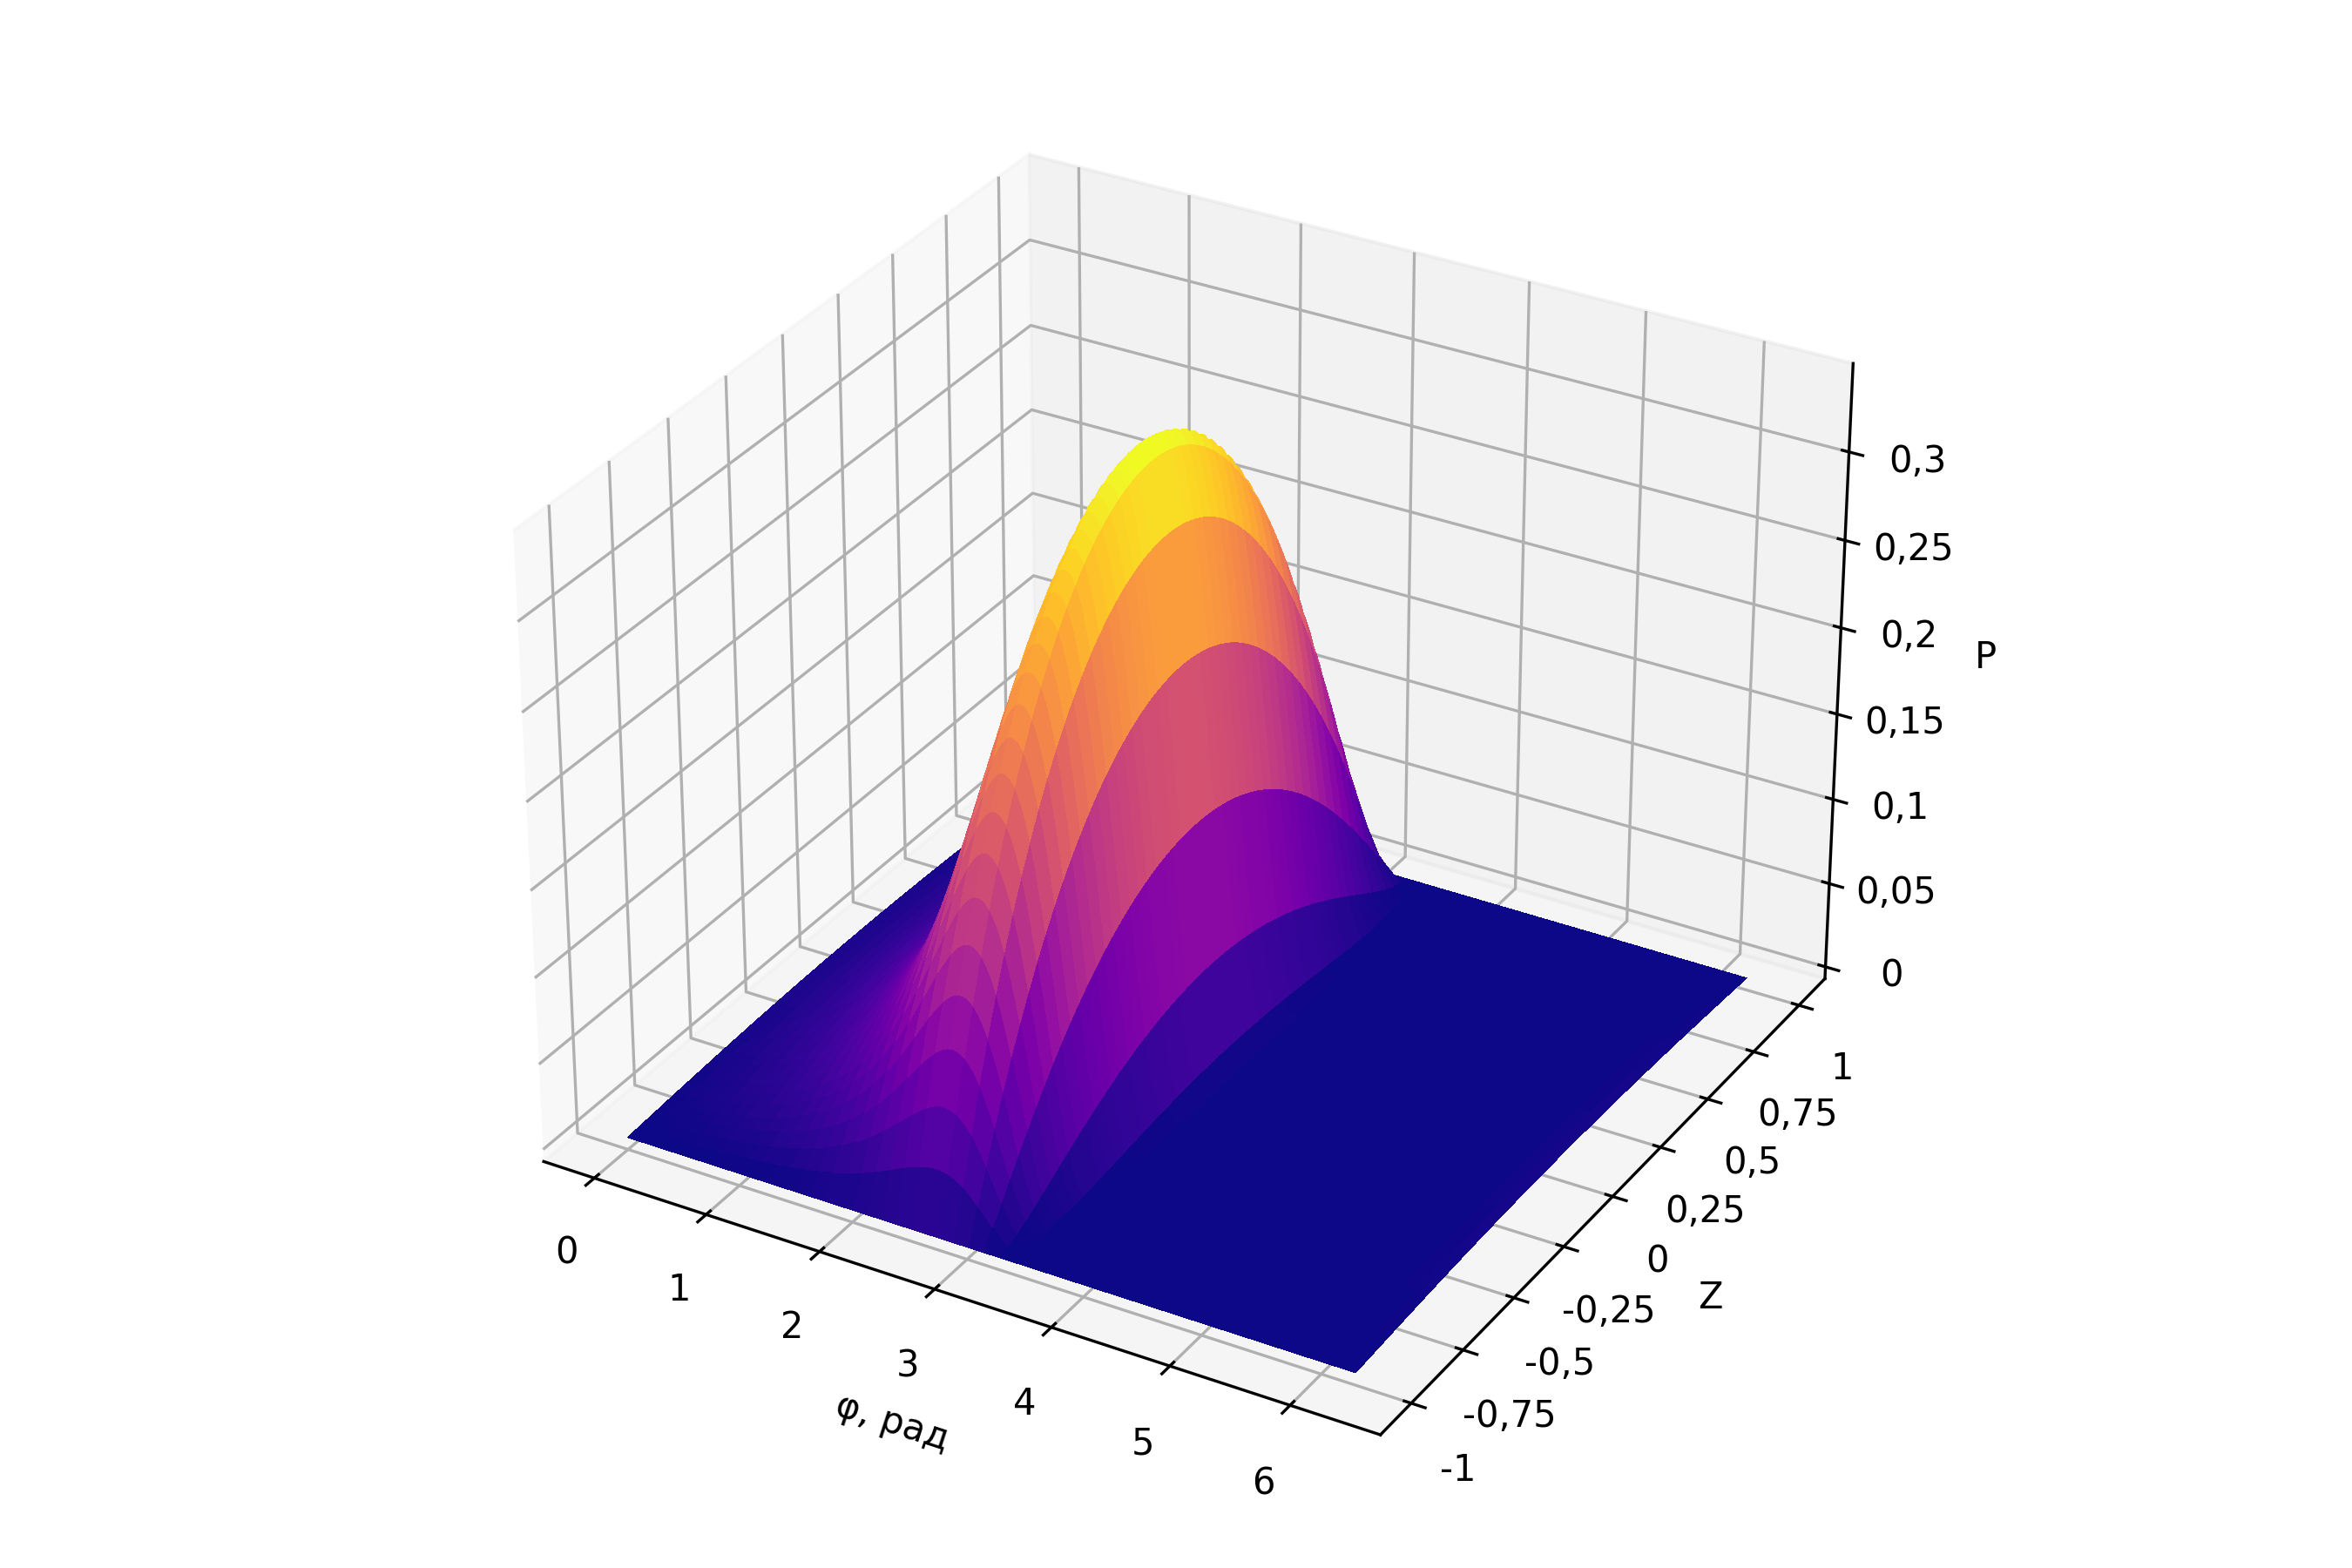
\includegraphics[width=0.75\textwidth]{figures/ch05/fig_5_3.png}
\caption{Поле безразмерного давления $P(\theta, Z)$
  гладкого подшипника при $\varepsilon = 0{,}6$.}
\label{fig:smooth_P3D}
\end{figure}

\begin{figure}[!ht]
\centering
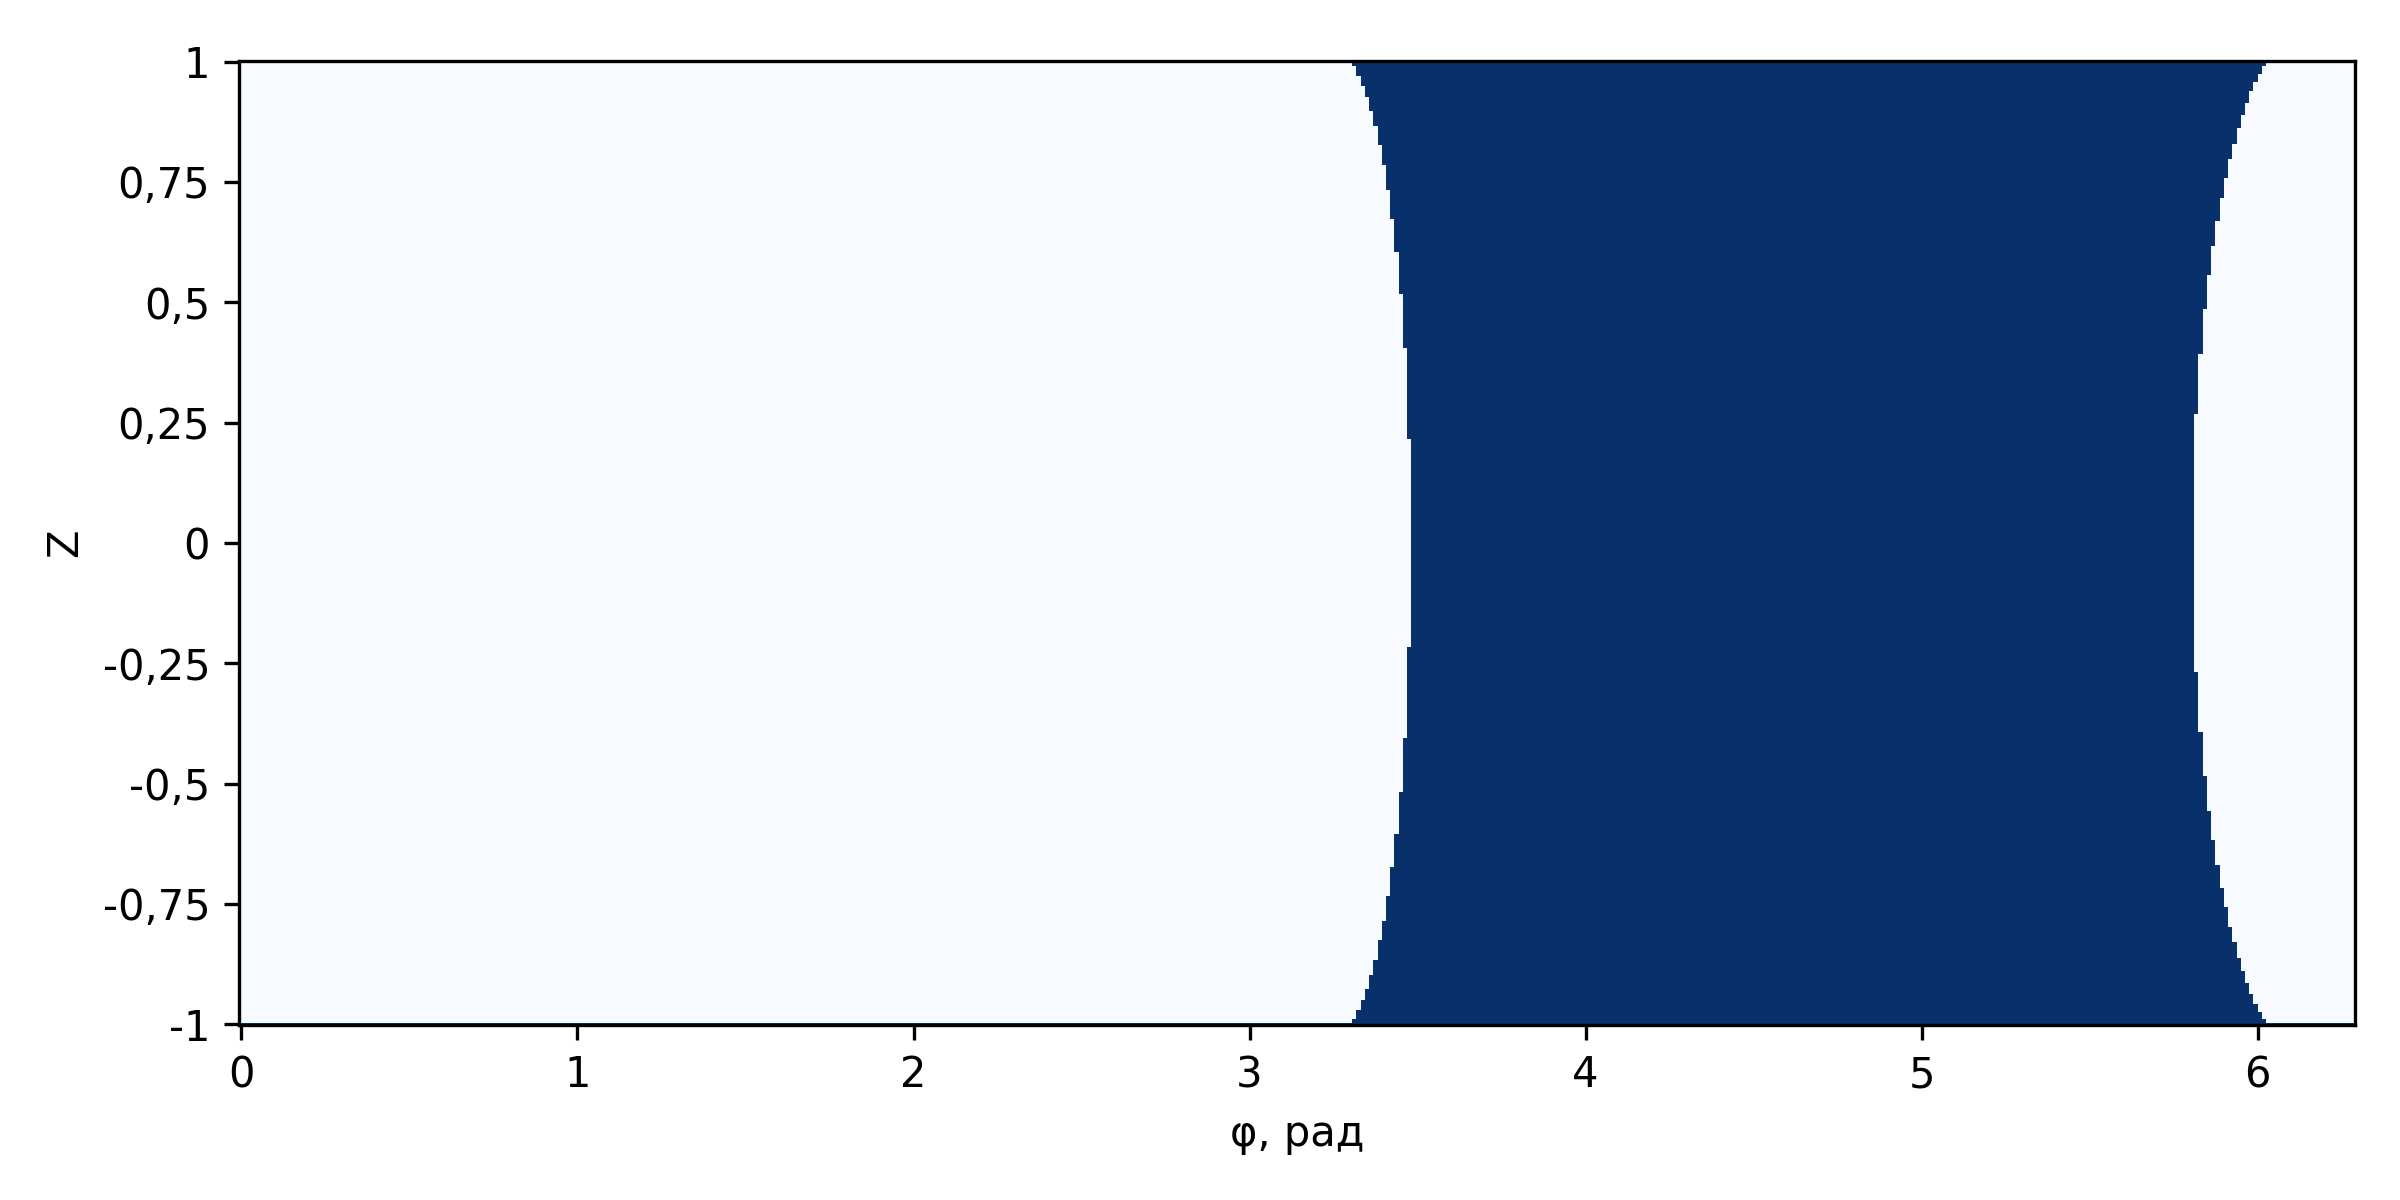
\includegraphics[width=0.75\textwidth]{figures/ch05/fig_5_4.png}
\caption{Карта кавитационной зоны гладкого подшипника
  при $\varepsilon = 0{,}6$. Область $P = 0$ выделена контрастным цветом.}
\label{fig:smooth_cav}
\end{figure}

\FloatBarrier

\textit{Интегральные характеристики.}
По полученному полю давления вычисляются интегральные
характеристики подшипника: компоненты несущей силы
и результирующая сила~$F$ с углом нагружения~$\varphi_{\mathrm{load}}$
(\eqref{eq:func_F_components}, \eqref{eq:func_psi}; в формуле~\eqref{eq:func_psi}
угол в общей постановке обозначен~$\psi$, в настоящей главе используется
обозначение~$\varphi_{\mathrm{load}}$, чтобы не путать с относительным
зазором $\psi = c/R$),
безразмерная сила трения~$f$ и коэффициент трения
$\mu_f = f/F$, а также осевые утечки~$Q_{\mathrm{out}}$
(\eqref{eq:func_Q_journal}). Значения указанных характеристик
при номинальном эксцентриситете приведены в
таблице~\ref{tab:smooth_results}.

\begin{table}[!ht]
\centering
\caption{Интегральные характеристики гладкого подшипника
  при $\varepsilon = \varepsilon_{\mathrm{nom}} = 0{,}6$}
\label{tab:smooth_results}
\begin{tabularx}{\textwidth}{|X|c|c|}
\hline
\multicolumn{1}{|c|}{\textbf{Характеристика}} & \textbf{Обозначение} & \textbf{Значение} \\
\hline
Несущая сила              & $F$, Н                        & 5035{,}7 \\
\hline
Угол нагружения           & $\varphi_{\mathrm{load}}$, $^{\circ}$ & 134{,}1 \\
\hline
Коэффициент трения        & $\mu_f$                       & 0{,}01537 \\
\hline
Осевые утечки             & $Q_{\mathrm{out}}$, мл/с      & 11{,}87 \\
\hline
\end{tabularx}
\end{table}

\FloatBarrier

\textit{Зависимости от эксцентриситета.}
Характерное поведение интегральных характеристик
гидродинамического подшипника при изменении эксцентриситета
определяется нелинейной зависимостью толщины зазора от~$\varepsilon$.
Несущая способность~$F(\varepsilon)$ монотонно возрастает
с ростом эксцентриситета, причём при $\varepsilon \to 1$
рост приобретает резко нелинейный характер, обусловленный
сужением минимального зазора и соответствующим увеличением
пиковых давлений. Коэффициент трения~$\mu_f(\varepsilon)$
убывает с ростом~$\varepsilon$: хотя абсолютные потери на трение
растут из-за повышения вязкого сдвига в зоне минимального зазора,
несущая способность растёт быстрее, и отношение~$\mu_f = f/F$
уменьшается. Осевые утечки~$Q_{\mathrm{out}}(\varepsilon)$
возрастают с ростом~$\varepsilon$: увеличение эксцентриситета
усиливает перепад давления в осевом направлении и расширяет зону
с ненулевым давлением, что приводит к росту осевого потока через
торцы подшипника. Указанные тенденции являются типичными
для гидродинамических подшипников и подтверждаются классическими
результатами. Графики зависимостей~$F(\varepsilon)$,
$\mu_f(\varepsilon)$ и~$Q_{\mathrm{out}}(\varepsilon)$ представлены
на рисунках~\ref{fig:F_vs_epsilon}, \ref{fig:mu_vs_epsilon},
\ref{fig:Q_vs_epsilon}.

\begin{figure}[!ht]
\centering
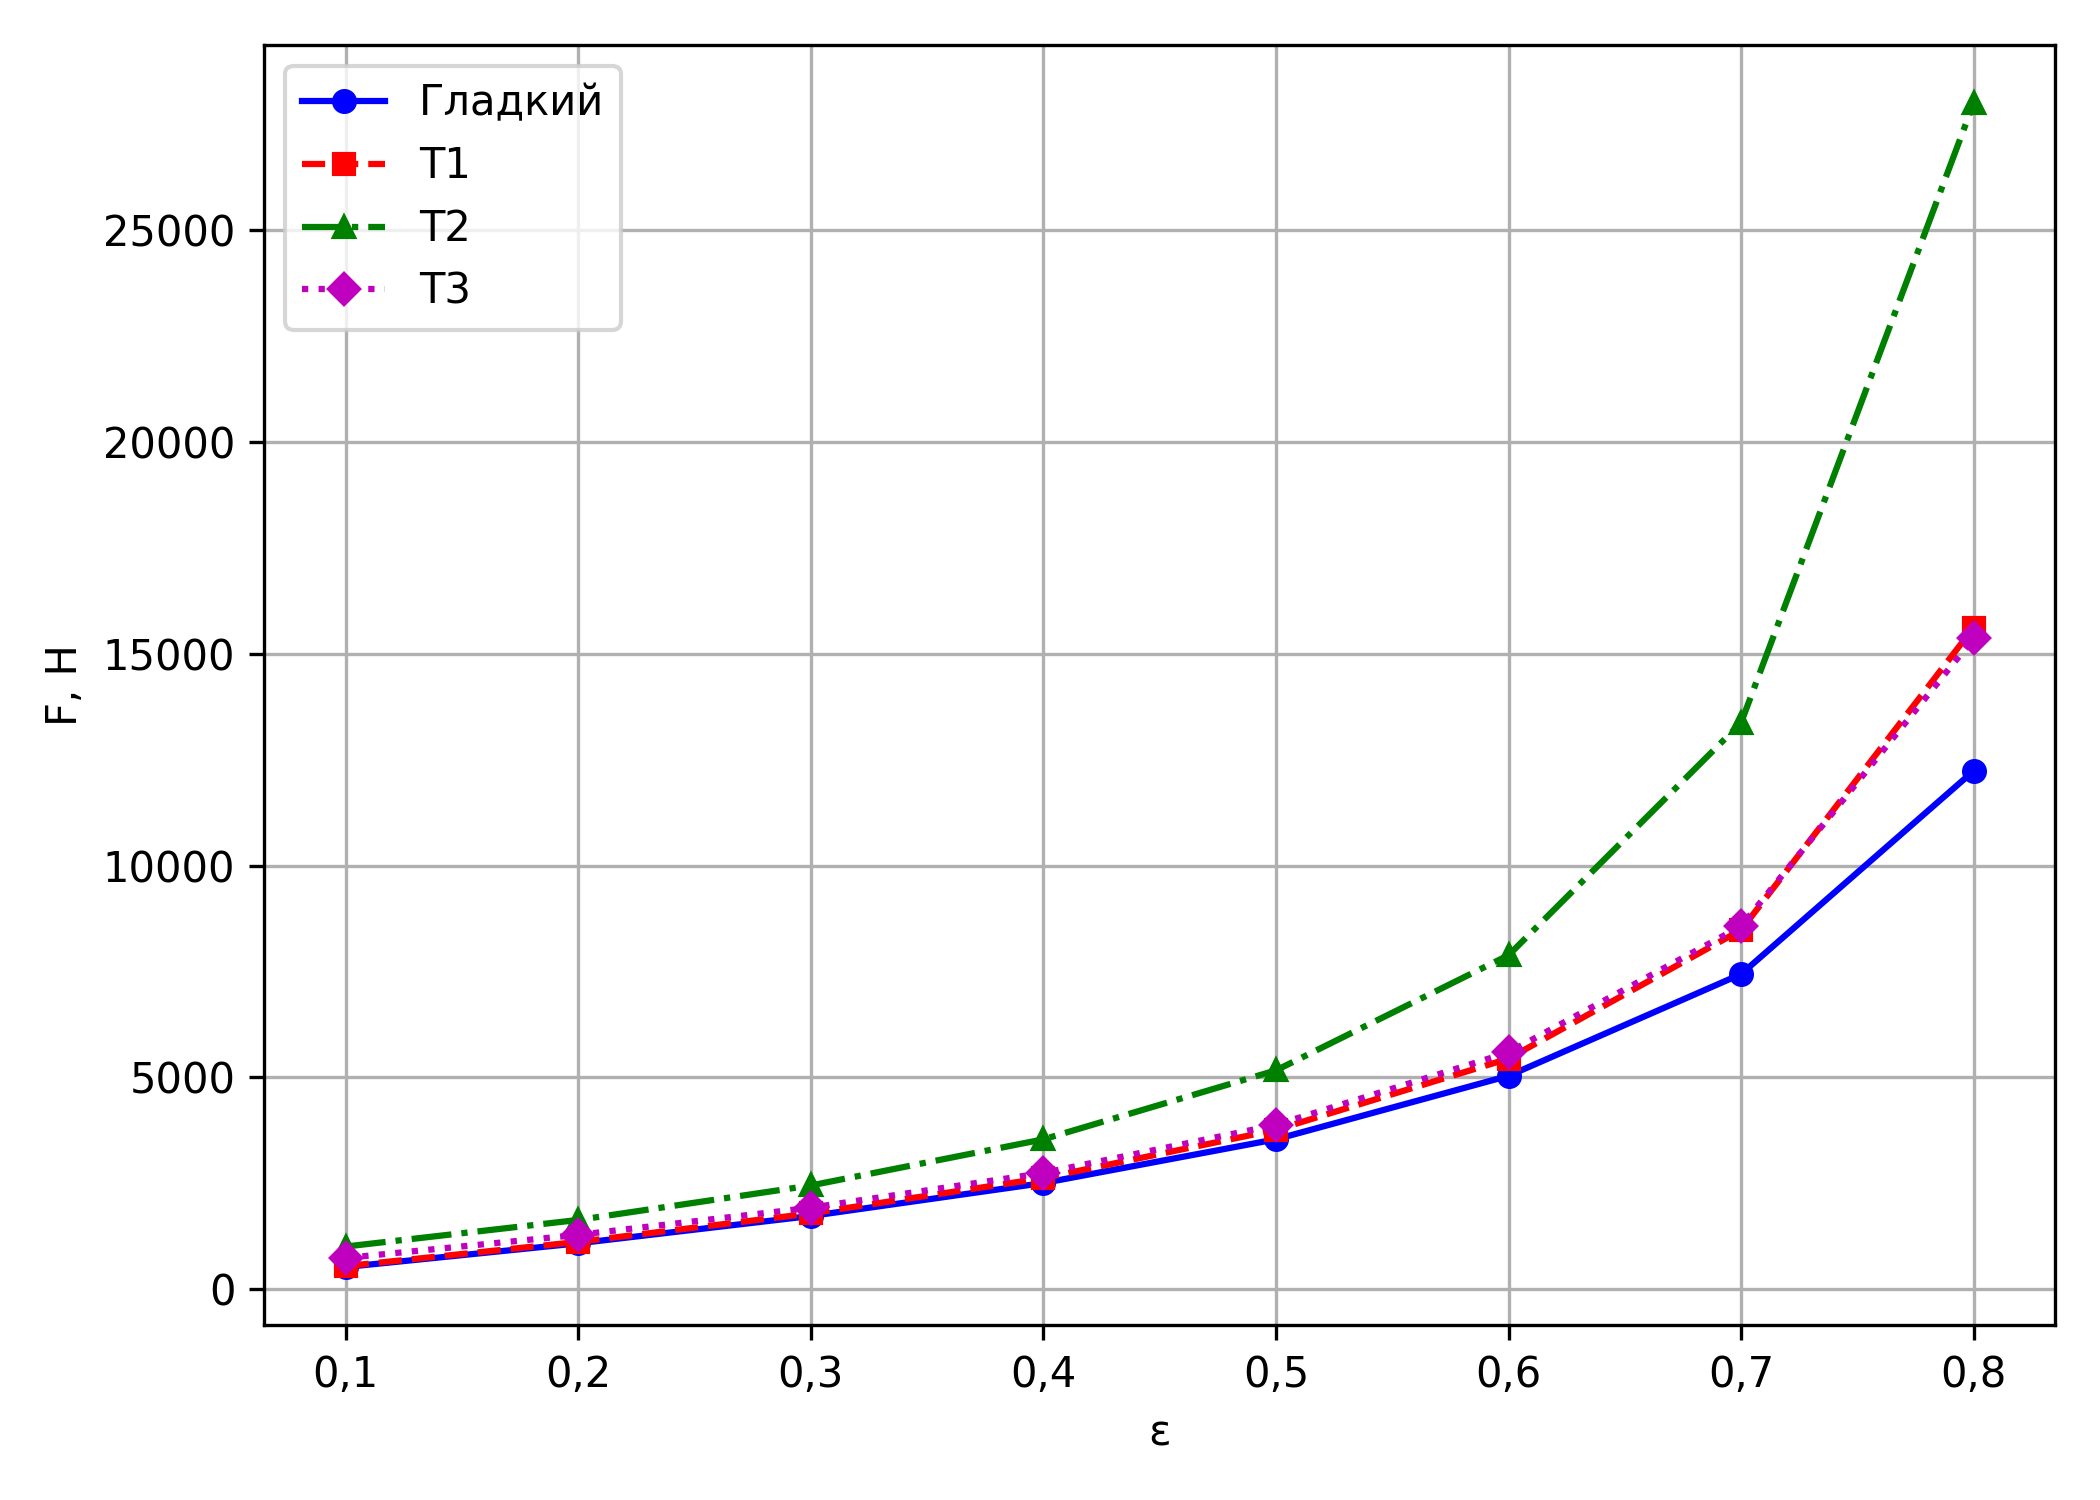
\includegraphics[width=0.75\textwidth]{figures/ch05/fig_5_5.png}
\caption{Зависимость несущей силы~$F$ от эксцентриситета~$\varepsilon$
  для гладкого подшипника и трёх конфигураций текстуры T1, T2, T3.}
\label{fig:F_vs_epsilon}
\end{figure}

\begin{figure}[!ht]
\centering
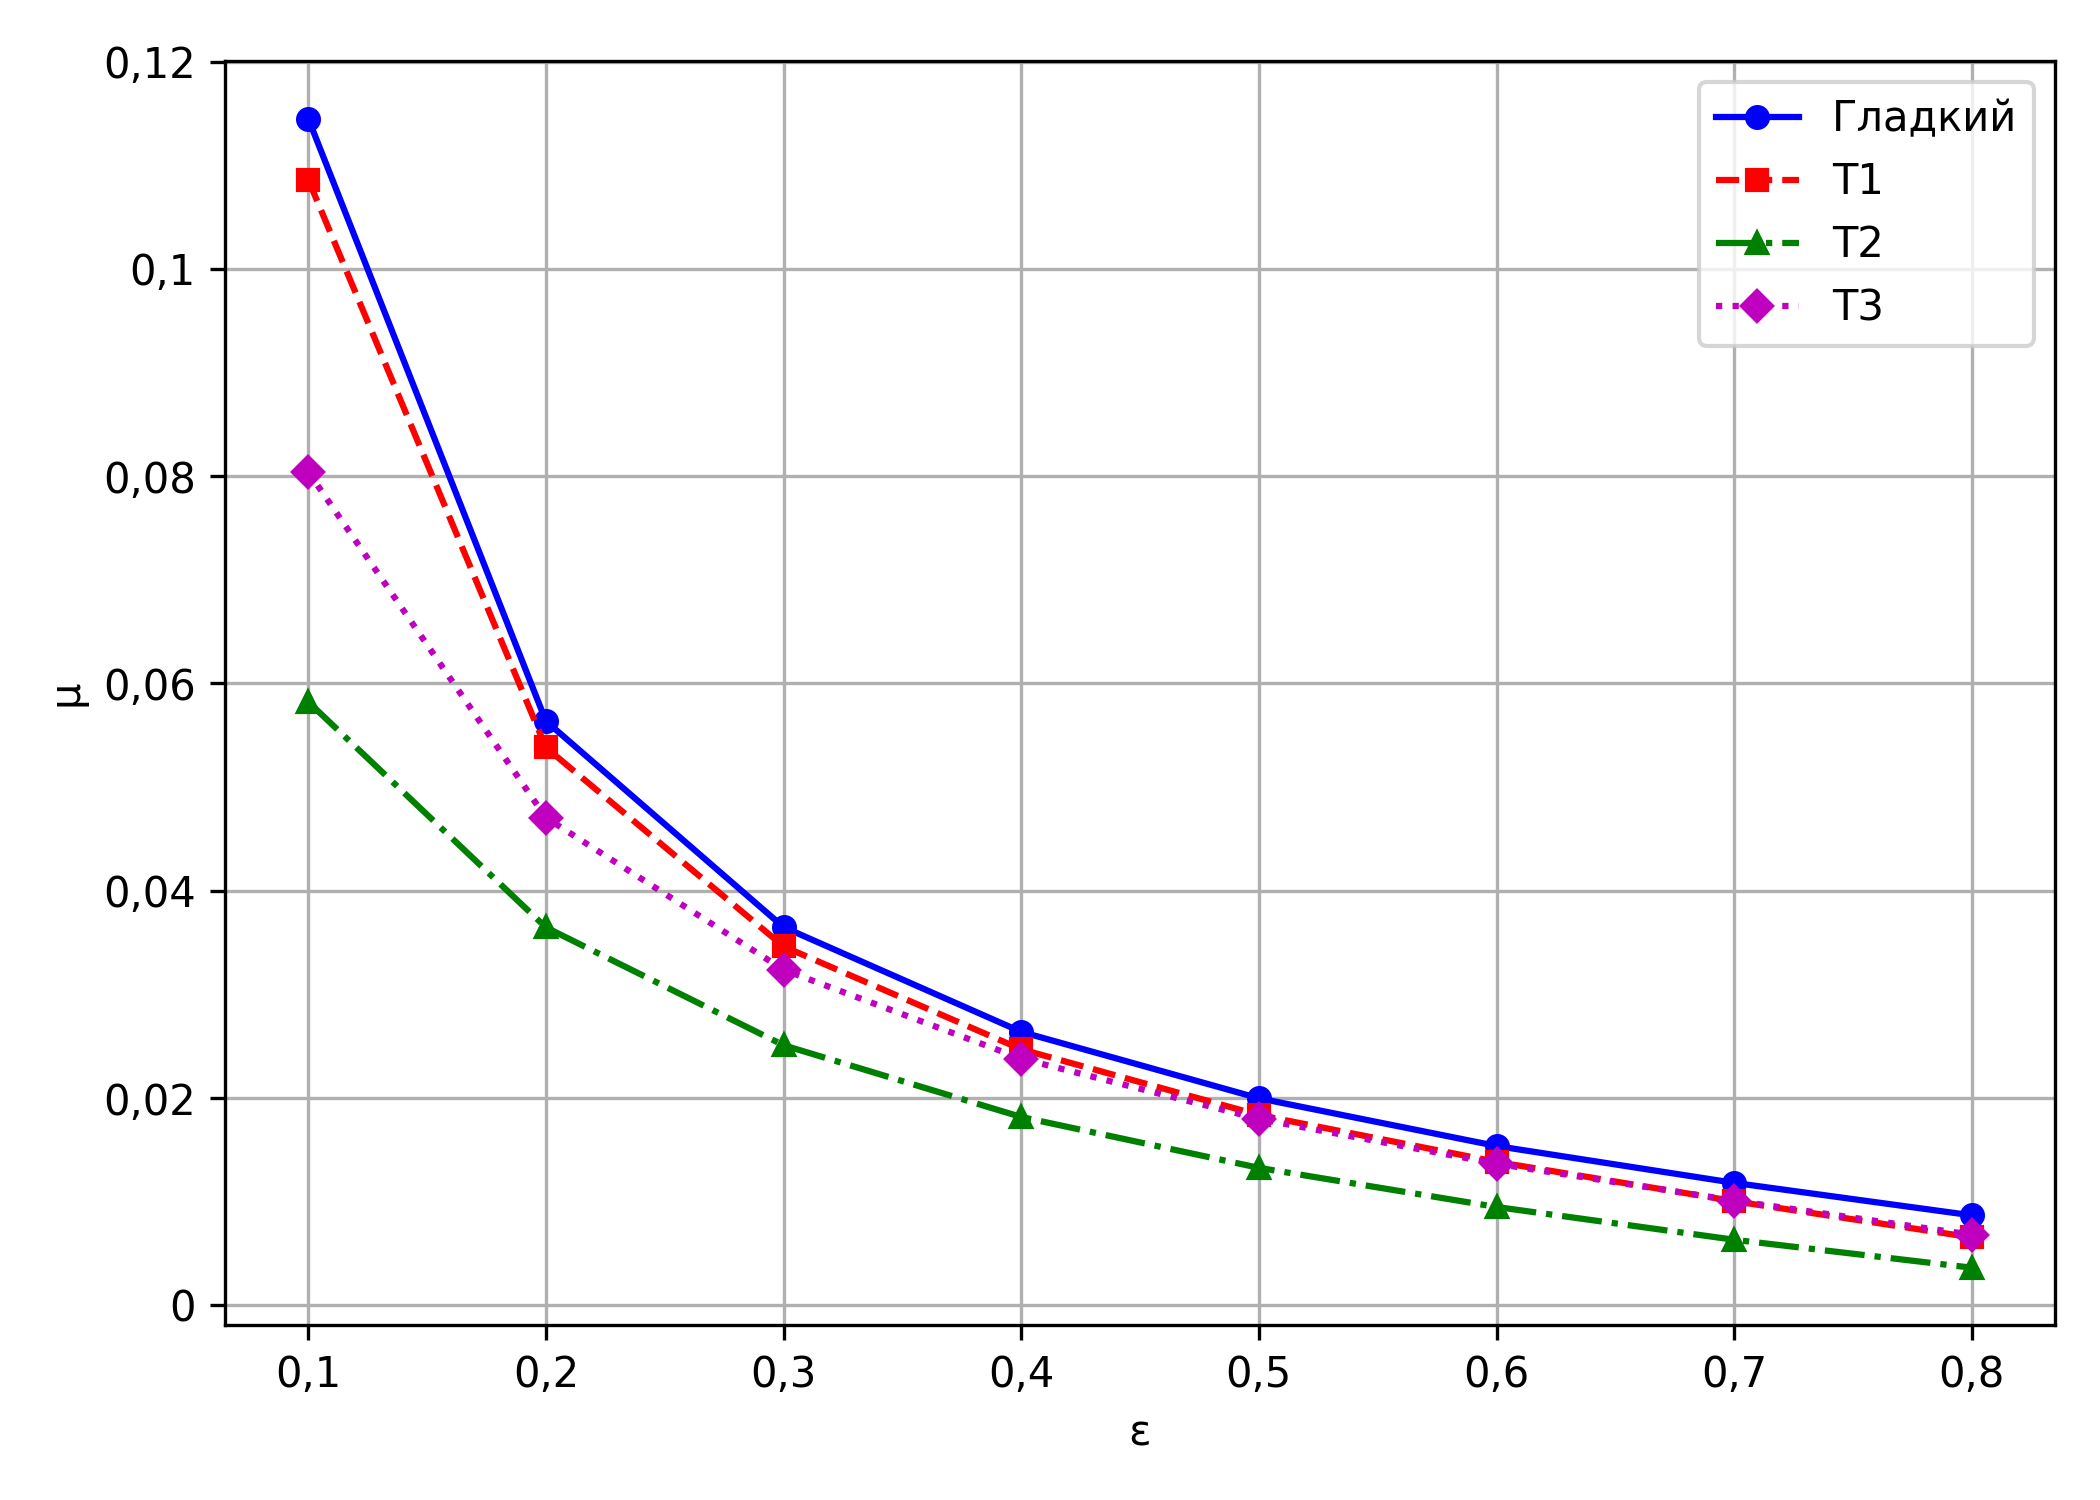
\includegraphics[width=0.75\textwidth]{figures/ch05/fig_5_6.png}
\caption{Зависимость коэффициента трения~$\mu_f$ от эксцентриситета~$\varepsilon$.}
\label{fig:mu_vs_epsilon}
\end{figure}

\begin{figure}[!htbp]
\centering
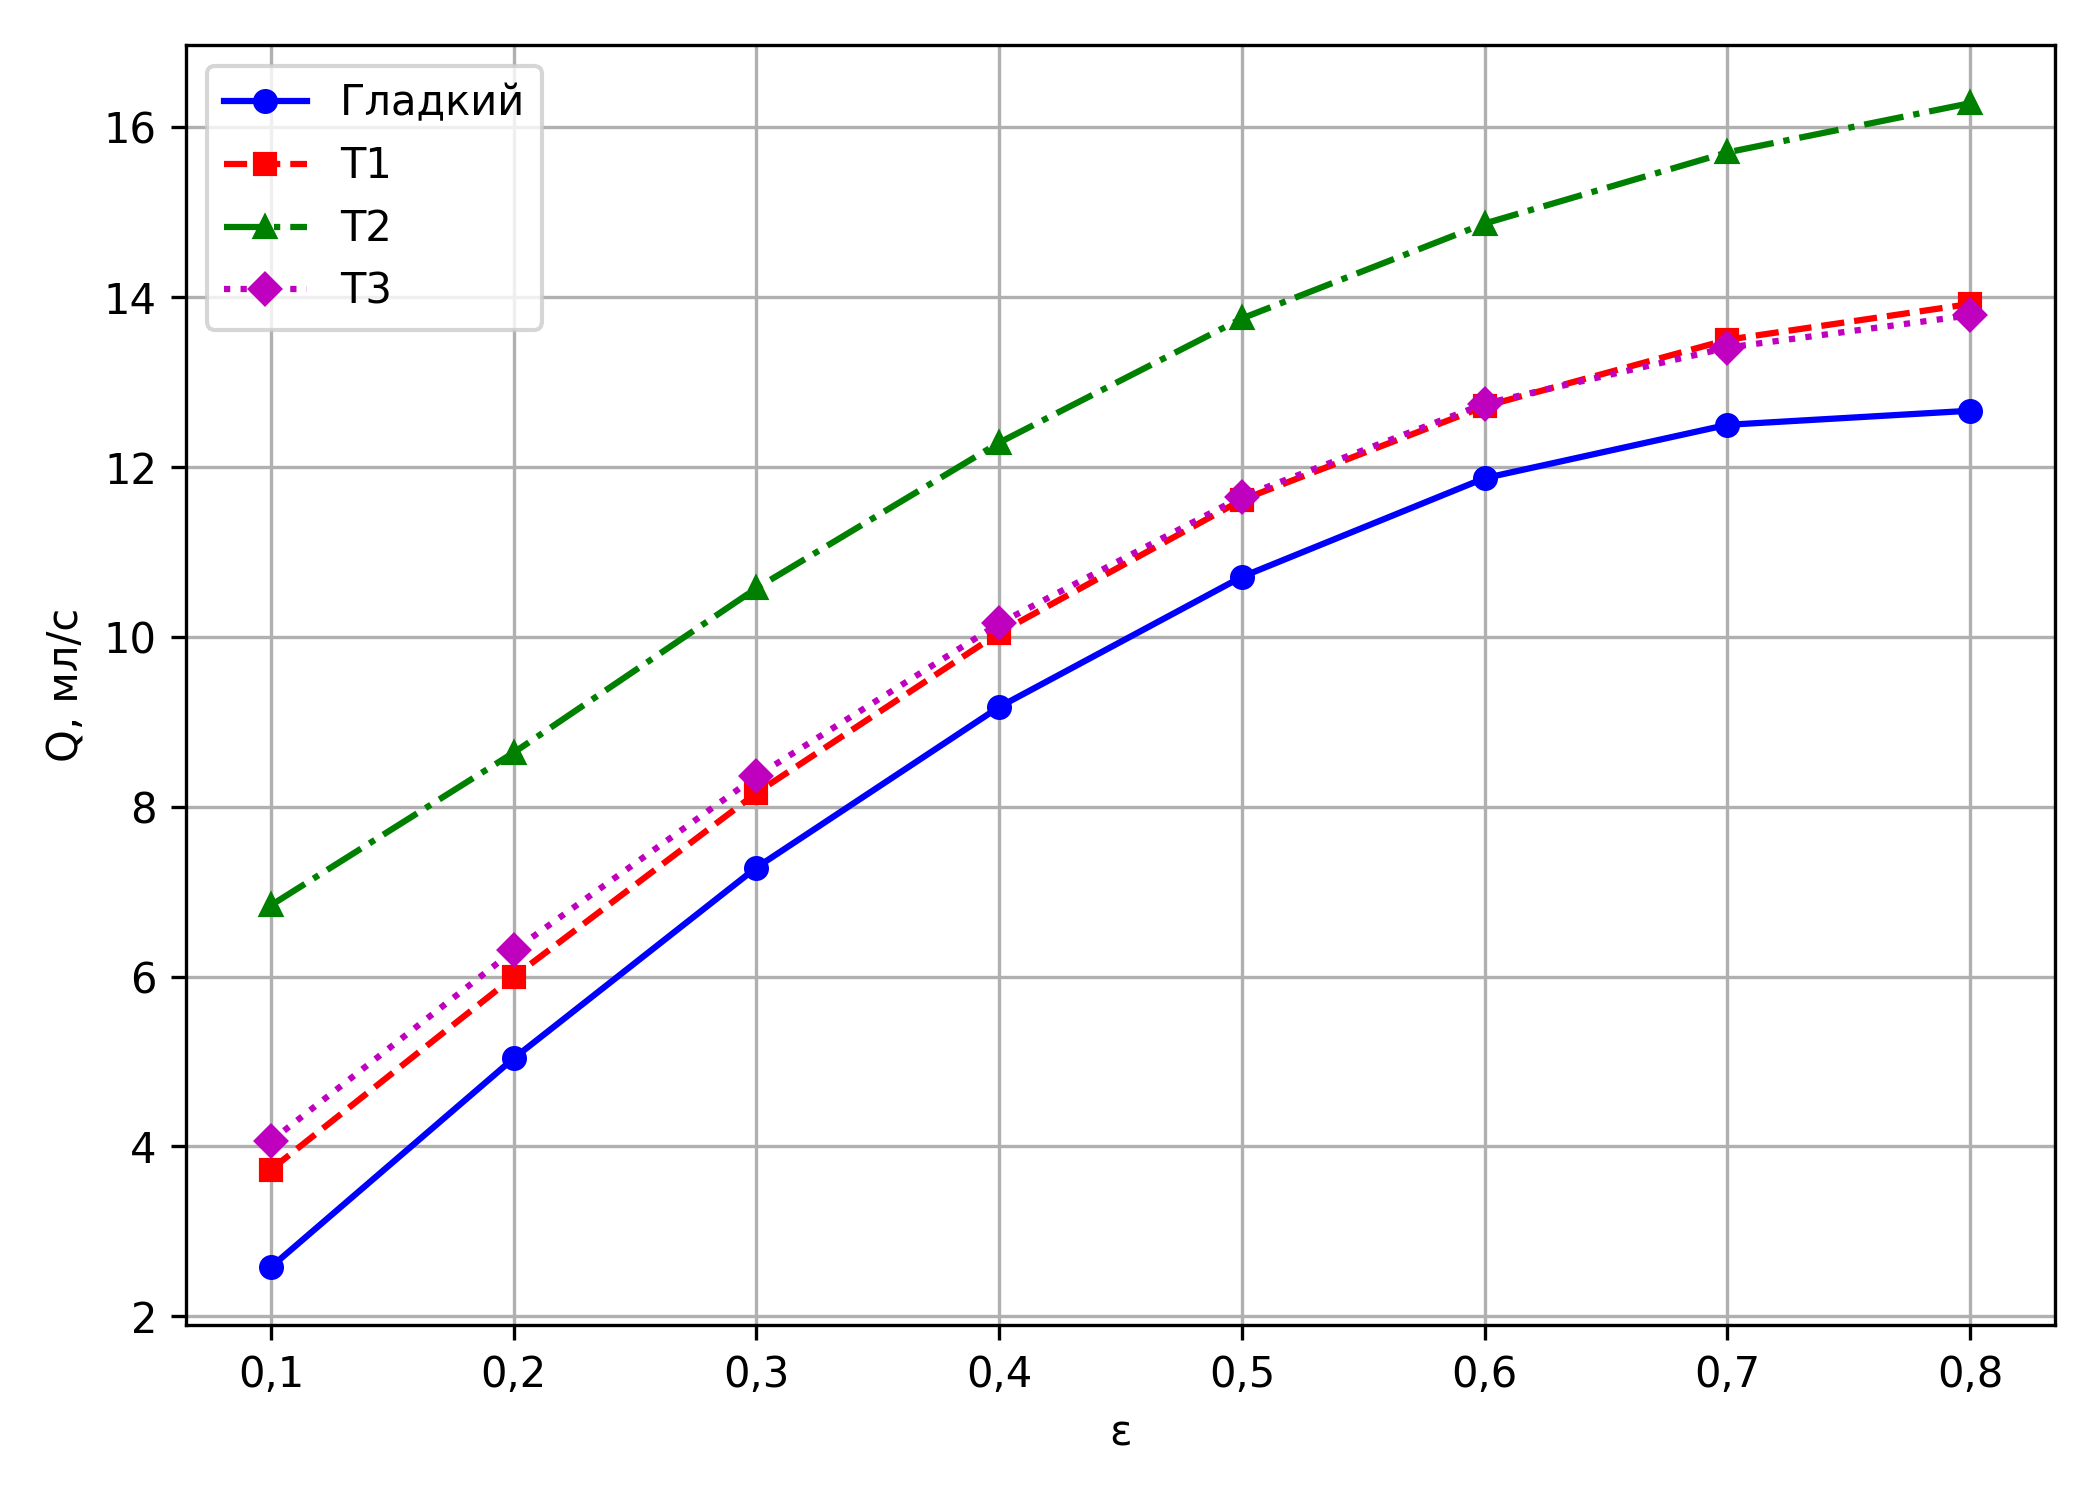
\includegraphics[width=0.75\textwidth]{figures/ch05/fig_5_7.png}
\caption{Зависимость осевых утечек~$Q_{\mathrm{out}}$ от эксцентриситета~$\varepsilon$.}
\label{fig:Q_vs_epsilon}
\end{figure}

\FloatBarrier

Полученные результаты для гладкого подшипника служат эталоном,
относительно которого оценивается влияние детерминированных
микроструктур в последующих разделах.

\section{Выбор и параметры микроструктуры}

В качестве элементов микрорельефа выбраны эллипсоидальные лунки
с профилем~\eqref{eq:profile_ellipsoidal}, представляющие
наиболее распространённый тип текстуры в задачах
гидродинамической смазки. Раскладка элементов выполнена
по шахматной схеме~\eqref{eq:layout_staggered}, обеспечивающей
равномерное заполнение текстурированной зоны при заданном
коэффициенте покрытия.

Выбор зоны нанесения микроструктур определяется физическим
механизмом их воздействия на поле давления. В радиальном
подшипнике текстурирование может охватывать всю поверхность
вкладыша, только зону сходящегося клина, зону максимального
давления или зону расходящегося клина. Расположение текстурированной
области относительно зоны давления существенно влияет на результат:
лунки в области сходящегося зазора способны усилить
гидродинамический эффект, тогда как лунки в зоне расходящегося
зазора могут расширить кавитационную область.

Безразмерные параметры текстуры определены в подразделе~2.2.4:
глубина элемента~$H_p$~\eqref{eq:Hp_nondim}, безразмерные
полуоси~$A^*$, $B^*$ и коэффициент покрытия~$\varphi$.
Рассматриваются три конфигурации текстуры, различающиеся
глубиной элементов и зоной нанесения
(таблица~\ref{tab:texture_configs}).

\begin{table}[!ht]
\centering
\caption{Параметры рассматриваемых конфигураций текстуры}
\label{tab:texture_configs}
\begin{tabularx}{\textwidth}{|X|c|c|c|c|c|}
\hline
\multicolumn{1}{|c|}{\textbf{Конфигурация}}   & $\boldsymbol{H_p}$ & $\boldsymbol{A^*}$ & $\boldsymbol{B^*}$   & $\boldsymbol{\varphi}$ & \textbf{Зона нанесения} \\
\hline
T1 & 0{,}20 & 0{,}0861 & 0{,}0633 & 0{,}240 & $90^{\circ}$--$270^{\circ}$ \\
\hline
T2 & 0{,}40 & 0{,}0861 & 0{,}0633 & 0{,}240 & $90^{\circ}$--$270^{\circ}$ \\
\hline
T3 & 0{,}20 & 0{,}0861 & 0{,}0633 & 0{,}240 & $0^{\circ}$--$180^{\circ}$ \\
\hline
\end{tabularx}
\end{table}

\FloatBarrier

Конфигурации T1 и T2 различаются глубиной лунок: T2 имеет вдвое
большую глубину ($H_p = 0{,}40$) при той же зоне нанесения
($90^{\circ}$--$270^{\circ}$). Сектор $90^{\circ}$--$270^{\circ}$
включает область минимального зазора ($\theta \approx \pi$)
и часть расходящегося участка. Конфигурация T3 отличается зоной
нанесения: лунки расположены в секторе $0^{\circ}$--$180^{\circ}$
(зона сходящегося клина) при глубине, совпадающей с T1.

Карта кавитационной зоны для конфигурации~T1, на которой различима
шахматная раскладка элементов, представлена на
рисунке~\ref{fig:texture_layout}.

\begin{figure}[!ht]
\centering
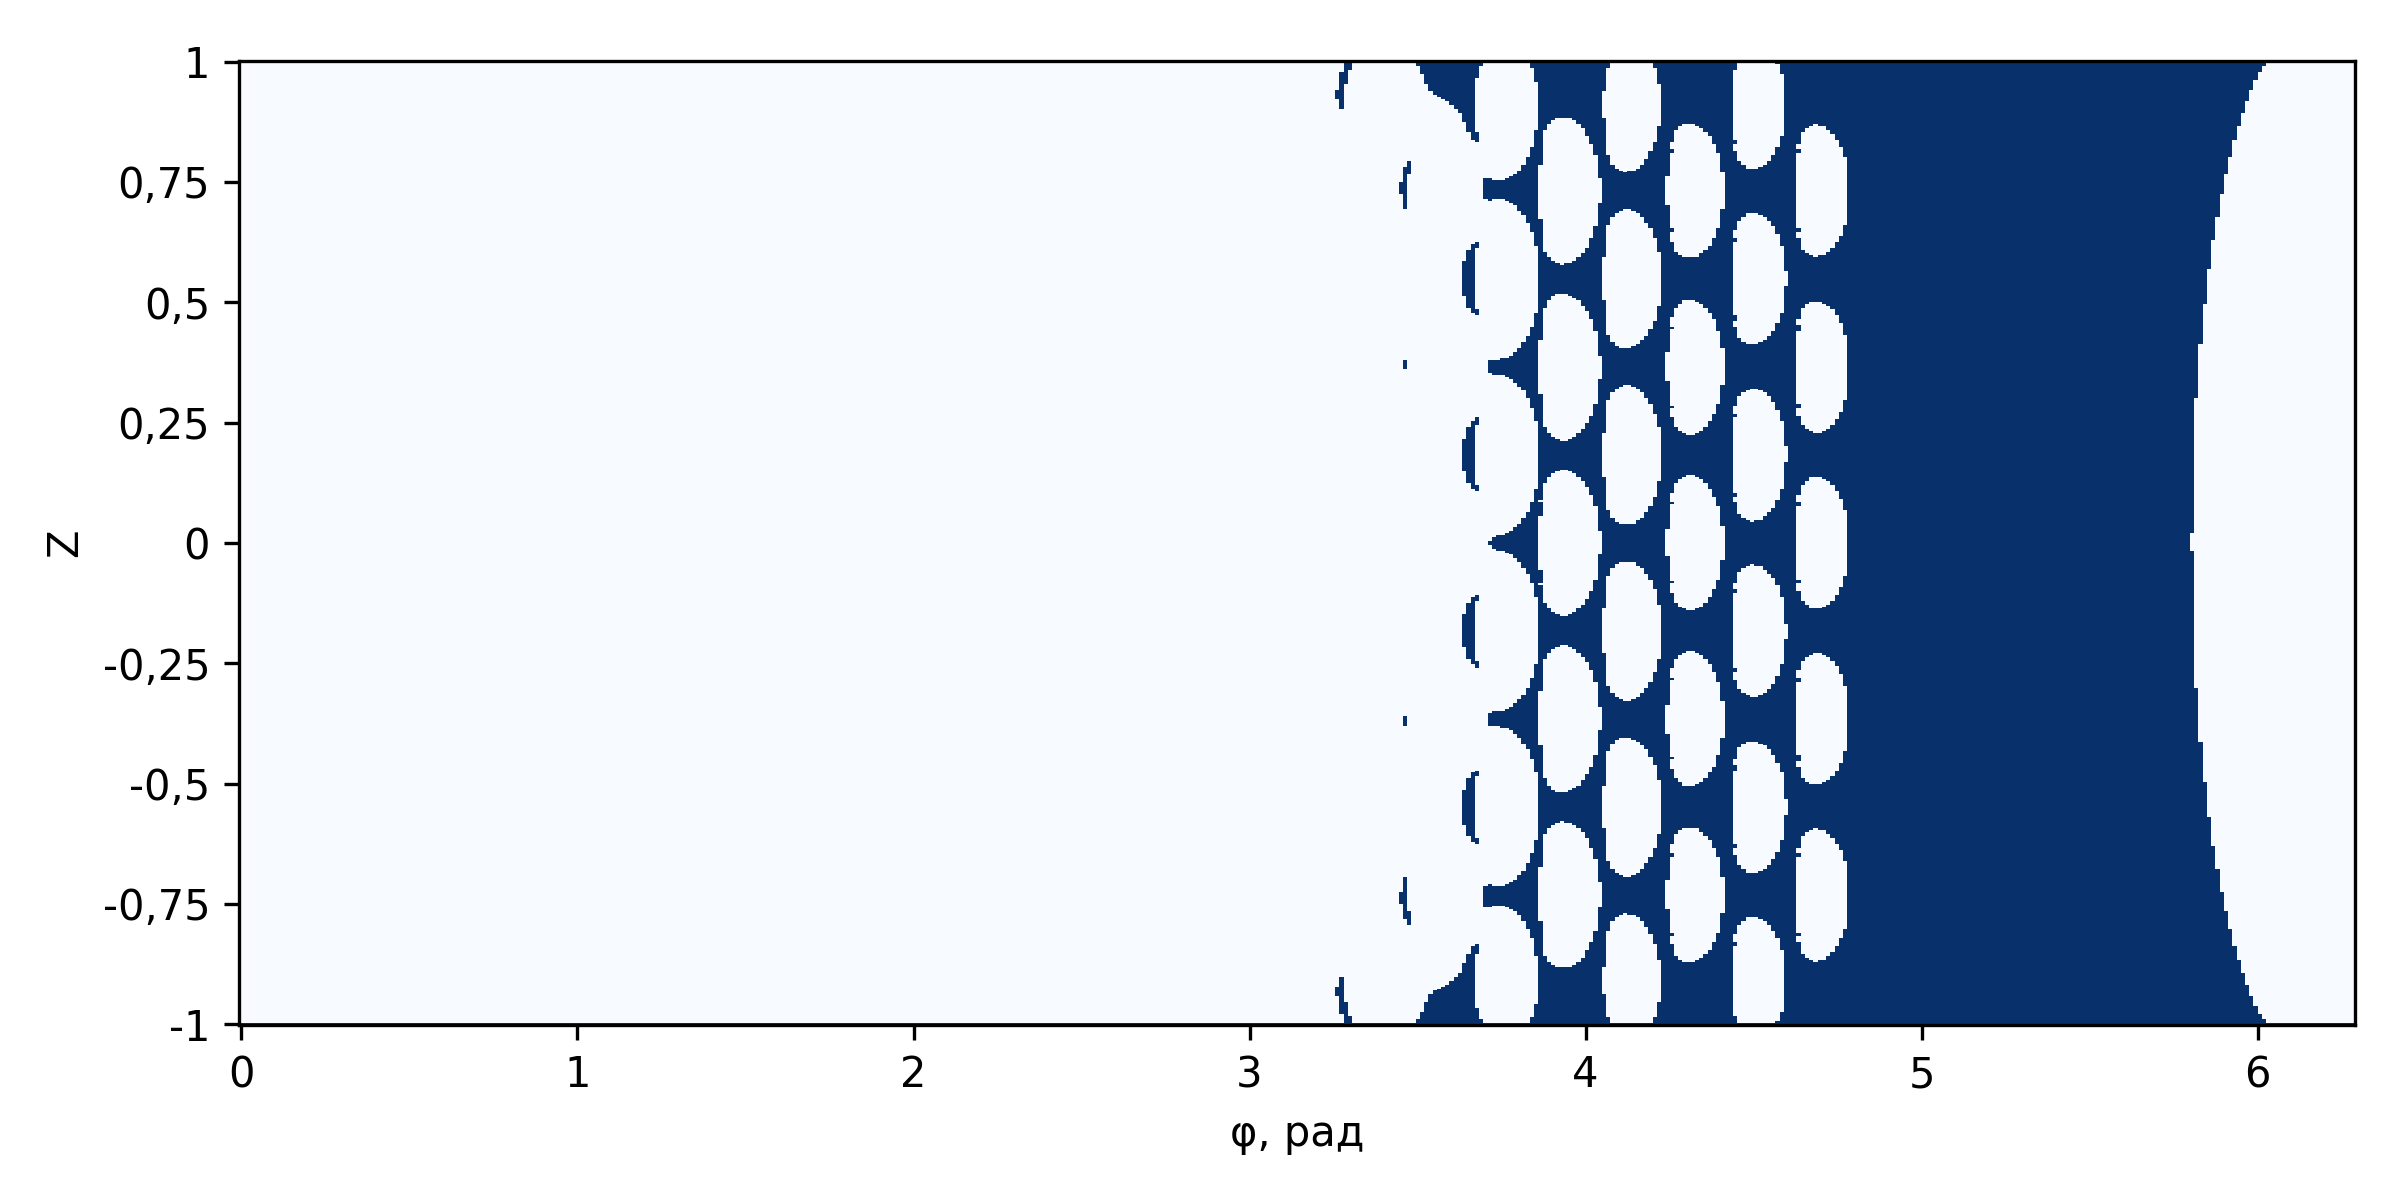
\includegraphics[width=0.75\textwidth]{figures/ch05/fig_5_8.png}
\caption{Карта кавитационной зоны текстурированного подшипника (конфигурация~T1,
  $\varepsilon = 0{,}6$). Шахматная раскладка элементов различима
  по локальным <<островкам>> зоны $P > 0$ внутри лунок.}
\label{fig:texture_layout}
\end{figure}


\section{Сравнение гладкого и текстурированного подшипников}

\textit{Физический механизм влияния микроструктур.}
Эллипсоидальные лунки, нанесённые на рабочую поверхность
вкладыша, создают локальные расширения и сужения зазора,
формируя дополнительные микроклинья. В зоне сходящегося
зазора подшипника, где давление формируется за счёт
макроскопического клинового эффекта~\eqref{eq:journal_h_ch5},
лунки создают дополнительные локальные области конвергенции,
что может усилить генерацию давления и повысить несущую
способность. В расходящейся зоне, где давление снижается
до уровня кавитации, лунки способны расширить кавитационную
область, изменяя баланс потоков на границе фазового перехода.
Результирующее влияние микроструктур на интегральные
характеристики определяется совокупностью этих эффектов
и зависит от зоны нанесения, глубины и коэффициента покрытия~$\varphi$.

\textit{Нормированные показатели эффективности.}
Для количественного сравнения текстурированного
и гладкого подшипников вводятся нормированные показатели:
\begin{equation}
\begin{split}
  &G_F = \frac{F_{\mathrm{tex}}}{F_{\mathrm{smooth}}}, \quad
  G_f = \frac{\mu_{f,\mathrm{tex}}}{\mu_{f,\mathrm{smooth}}}, \\
  &G_Q = \frac{Q_{\mathrm{out,tex}}}{Q_{\mathrm{out,smooth}}}, \quad
  G_h = \frac{h_{\min,\mathrm{tex}}}{h_{\min,\mathrm{smooth}}}.
\end{split}
  \label{eq:gain_factors}
\end{equation}
Значение~$G > 1$ указывает на рост соответствующего показателя
при текстурировании, $G < 1$~-- на снижение. С точки зрения
эксплуатации желательны~$G_F > 1$ (рост несущей способности),
$G_f < 1$ (снижение трения) и $G_h > 1$ (увеличение минимального
зазора, повышение запаса по толщине плёнки).

\textit{Интегральные характеристики при номинальном эксцентриситете.}
Результаты расчёта для гладкого подшипника и трёх конфигураций
текстуры при $\varepsilon = 0{,}6$ сведены в
таблицу~\ref{tab:comparison_results}.

\begin{table}[!ht]
\centering
\caption{Интегральные характеристики подшипников при $\varepsilon = 0{,}6$}
\label{tab:comparison_results}
\resizebox{\textwidth}{!}{%
\begin{tabular}{|l|c|c|c|c|c|c|c|c|}
\hline
\multicolumn{1}{|c|}{\textbf{Вариант}} & $\boldsymbol{F}$, \textbf{Н} & $\boldsymbol{\varphi_{\mathrm{load}}}$, $\boldsymbol{^{\circ}}$ & $\boldsymbol{\mu_f}$ & $\boldsymbol{Q_{\mathrm{out}}}$, \textbf{мл/с} & $\boldsymbol{G_F}$ & $\boldsymbol{G_f}$ & $\boldsymbol{G_Q}$ & $\boldsymbol{G_h}$ \\
\hline
Гладкий & 5035{,}7 & 134{,}1 & 0{,}01537 & 11{,}87 & --- & --- & --- & --- \\
\hline
T1 & 5443{,}2 & 139{,}3 & 0{,}01384 & 12{,}72 & 1{,}081 & 0{,}900 & 1{,}071 & 1{,}00 \\
\hline
T2 & 7884{,}5 & 150{,}3 & 0{,}00949 & 14{,}87 & 1{,}566 & 0{,}617 & 1{,}253 & 1{,}00 \\
\hline
T3 & 5588{,}9 & 139{,}4 & 0{,}01366 & 12{,}75 & 1{,}110 & 0{,}888 & 1{,}074 & 1{,}00 \\
\hline
\end{tabular}%
}
\end{table}

\FloatBarrier

Конфигурация T2 демонстрирует наибольший прирост несущей
способности ($G_F = 1{,}566$) и наибольшее снижение коэффициента
трения ($G_f = 0{,}617$), однако сопровождается существенным
увеличением осевых утечек ($G_Q = 1{,}253$). Конфигурации T1 и T3
показывают близкие результаты, что свидетельствует о меньшей
чувствительности характеристик к зоне нанесения при умеренной
глубине лунок ($H_p = 0{,}20$).

Показатель $G_h = 1{,}00$ для всех конфигураций означает, что
глобальный минимум толщины плёнки в расчёте достигается вне лунок:
вследствие дискретного покрытия поверхности $\min H(\theta,Z)
= 1 - \varepsilon$, и минимальный зазор определяется исключительно
эксцентриситетом.

Нормированные показатели эффективности для трёх конфигураций
наглядно сопоставлены на рисунке~\ref{fig:gains_nom}.

\textit{Поля давления и кавитация.}
Текстурирование поверхности вкладыша модифицирует распределение
давления в смазочном слое. В области расположения лунок поле
давления приобретает локальные возмущения~-- каждый элемент
микрорельефа формирует собственный микроклин, вносящий вклад
в интегральный баланс. Одновременно изменяется конфигурация
кавитационной области: распределение зон $P = 0$ и их суммарная
площадь зависят от параметров текстуры. Сопоставление
полей давления и карт кавитации для гладкого
и текстурированного подшипников при одинаковом значении
эксцентриситета представлено на
рисунках~\ref{fig:P3D_T1}, \ref{fig:texture_layout}, \ref{fig:P3D_T2}, \ref{fig:cav_T2}, \ref{fig:P3D_T3}, \ref{fig:cav_T3}.

\begin{figure}[!ht]
\centering
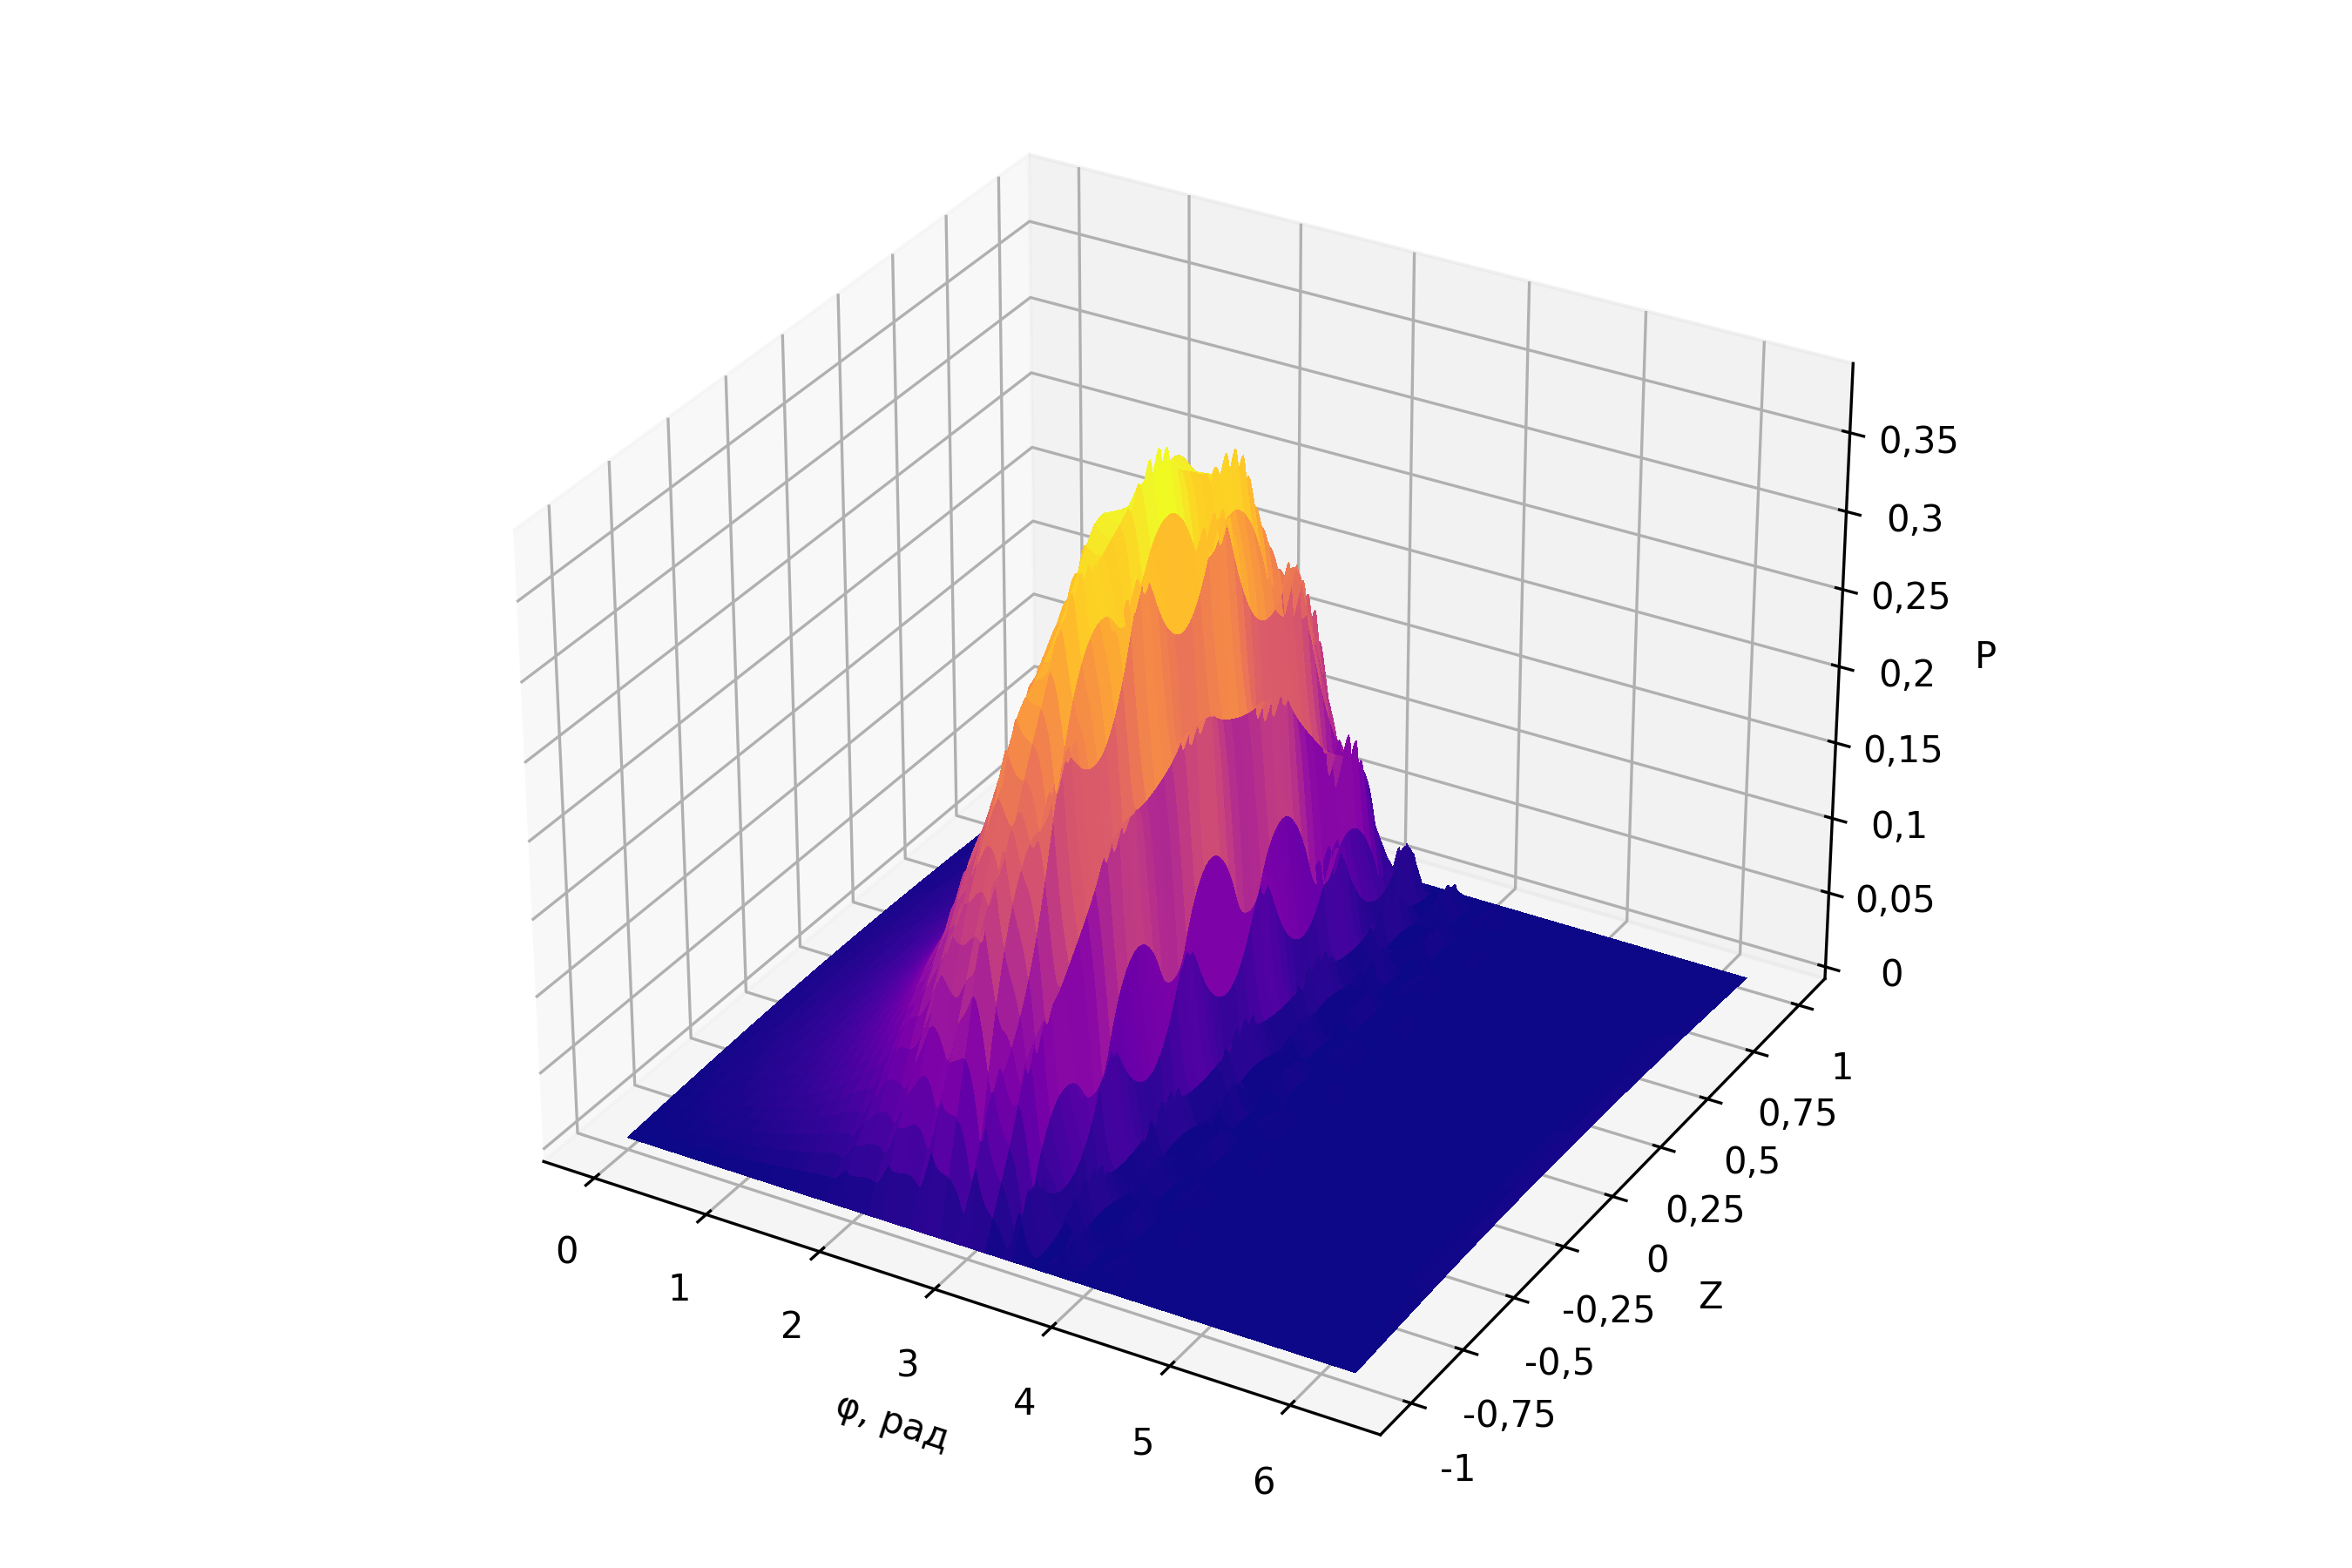
\includegraphics[width=0.75\textwidth]{figures/ch05/fig_5_9.png}
\caption{Поле давления $P(\theta, Z)$ для конфигурации~T1
  ($H_p = 0{,}20$, зона $90^{\circ}$--$270^{\circ}$)
  при $\varepsilon = 0{,}6$.}
\label{fig:P3D_T1}
\end{figure}


\begin{figure}[!ht]
\centering
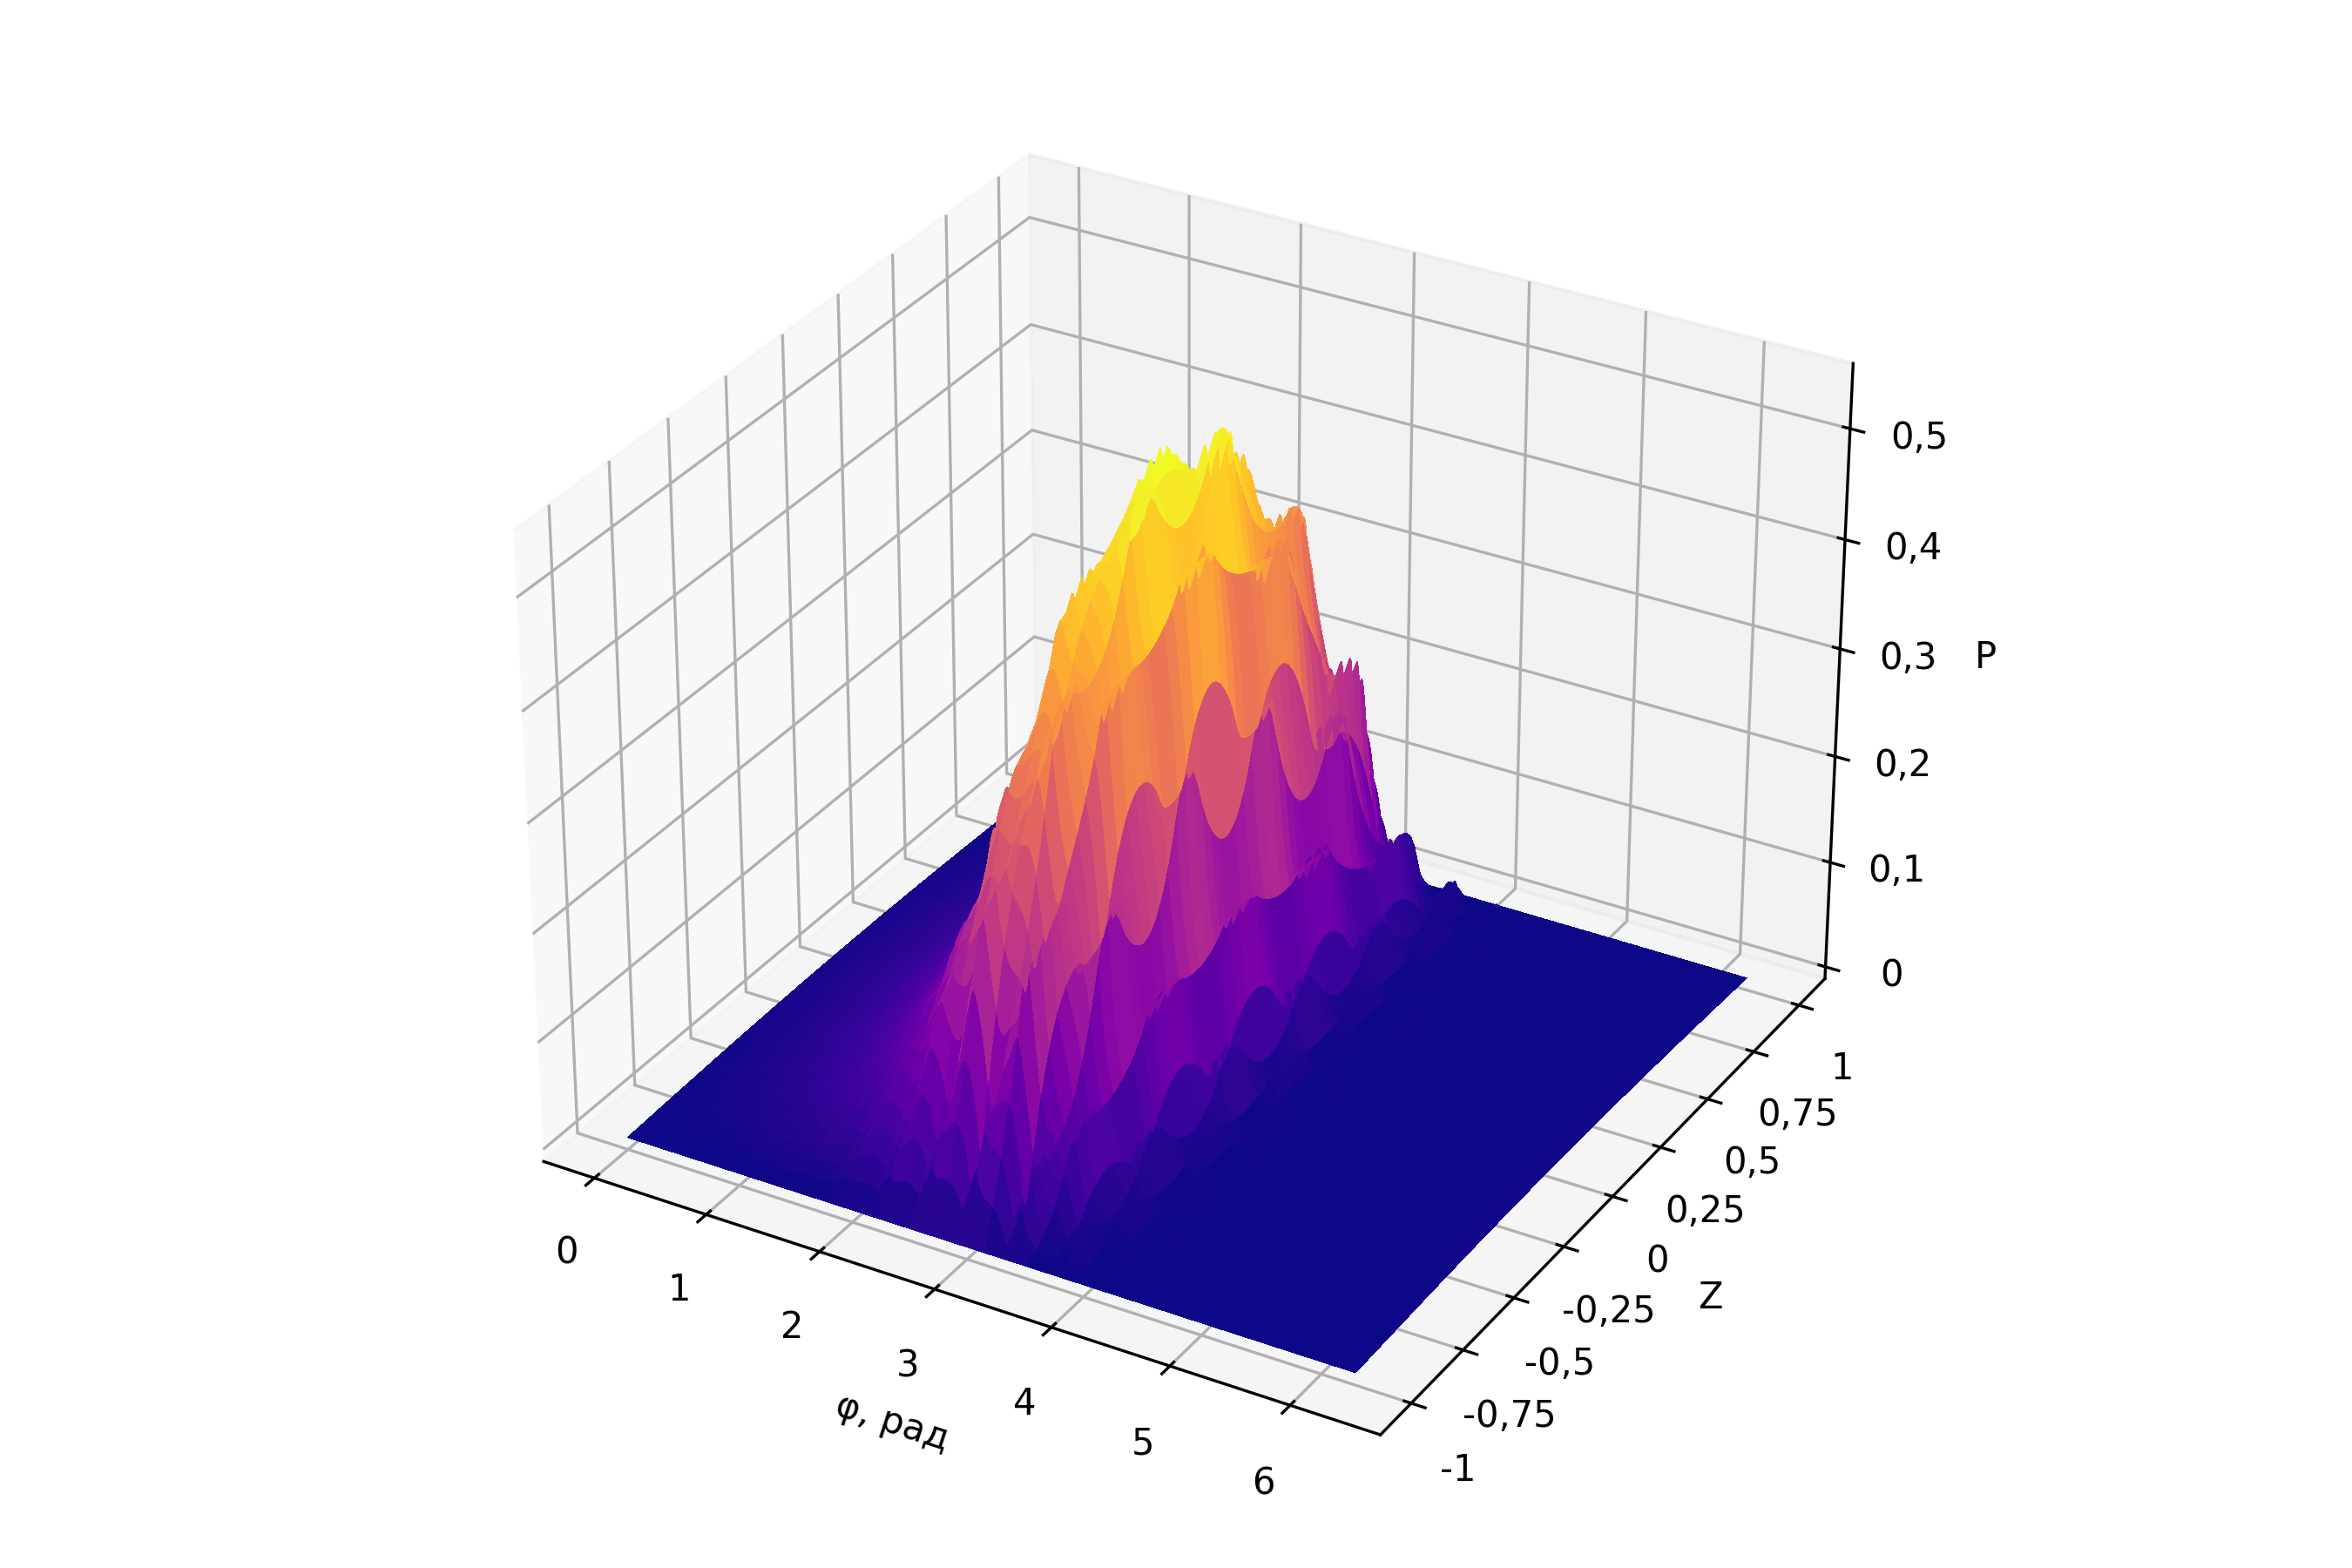
\includegraphics[width=0.75\textwidth]{figures/ch05/fig_5_10.png}
\caption{Поле давления $P(\theta, Z)$ для конфигурации~T2
  ($H_p = 0{,}40$, зона $90^{\circ}$--$270^{\circ}$)
  при $\varepsilon = 0{,}6$. Увеличение глубины лунок приводит
  к более выраженной ряби на поверхности давления.}
\label{fig:P3D_T2}
\end{figure}

\begin{figure}[!ht]
\centering
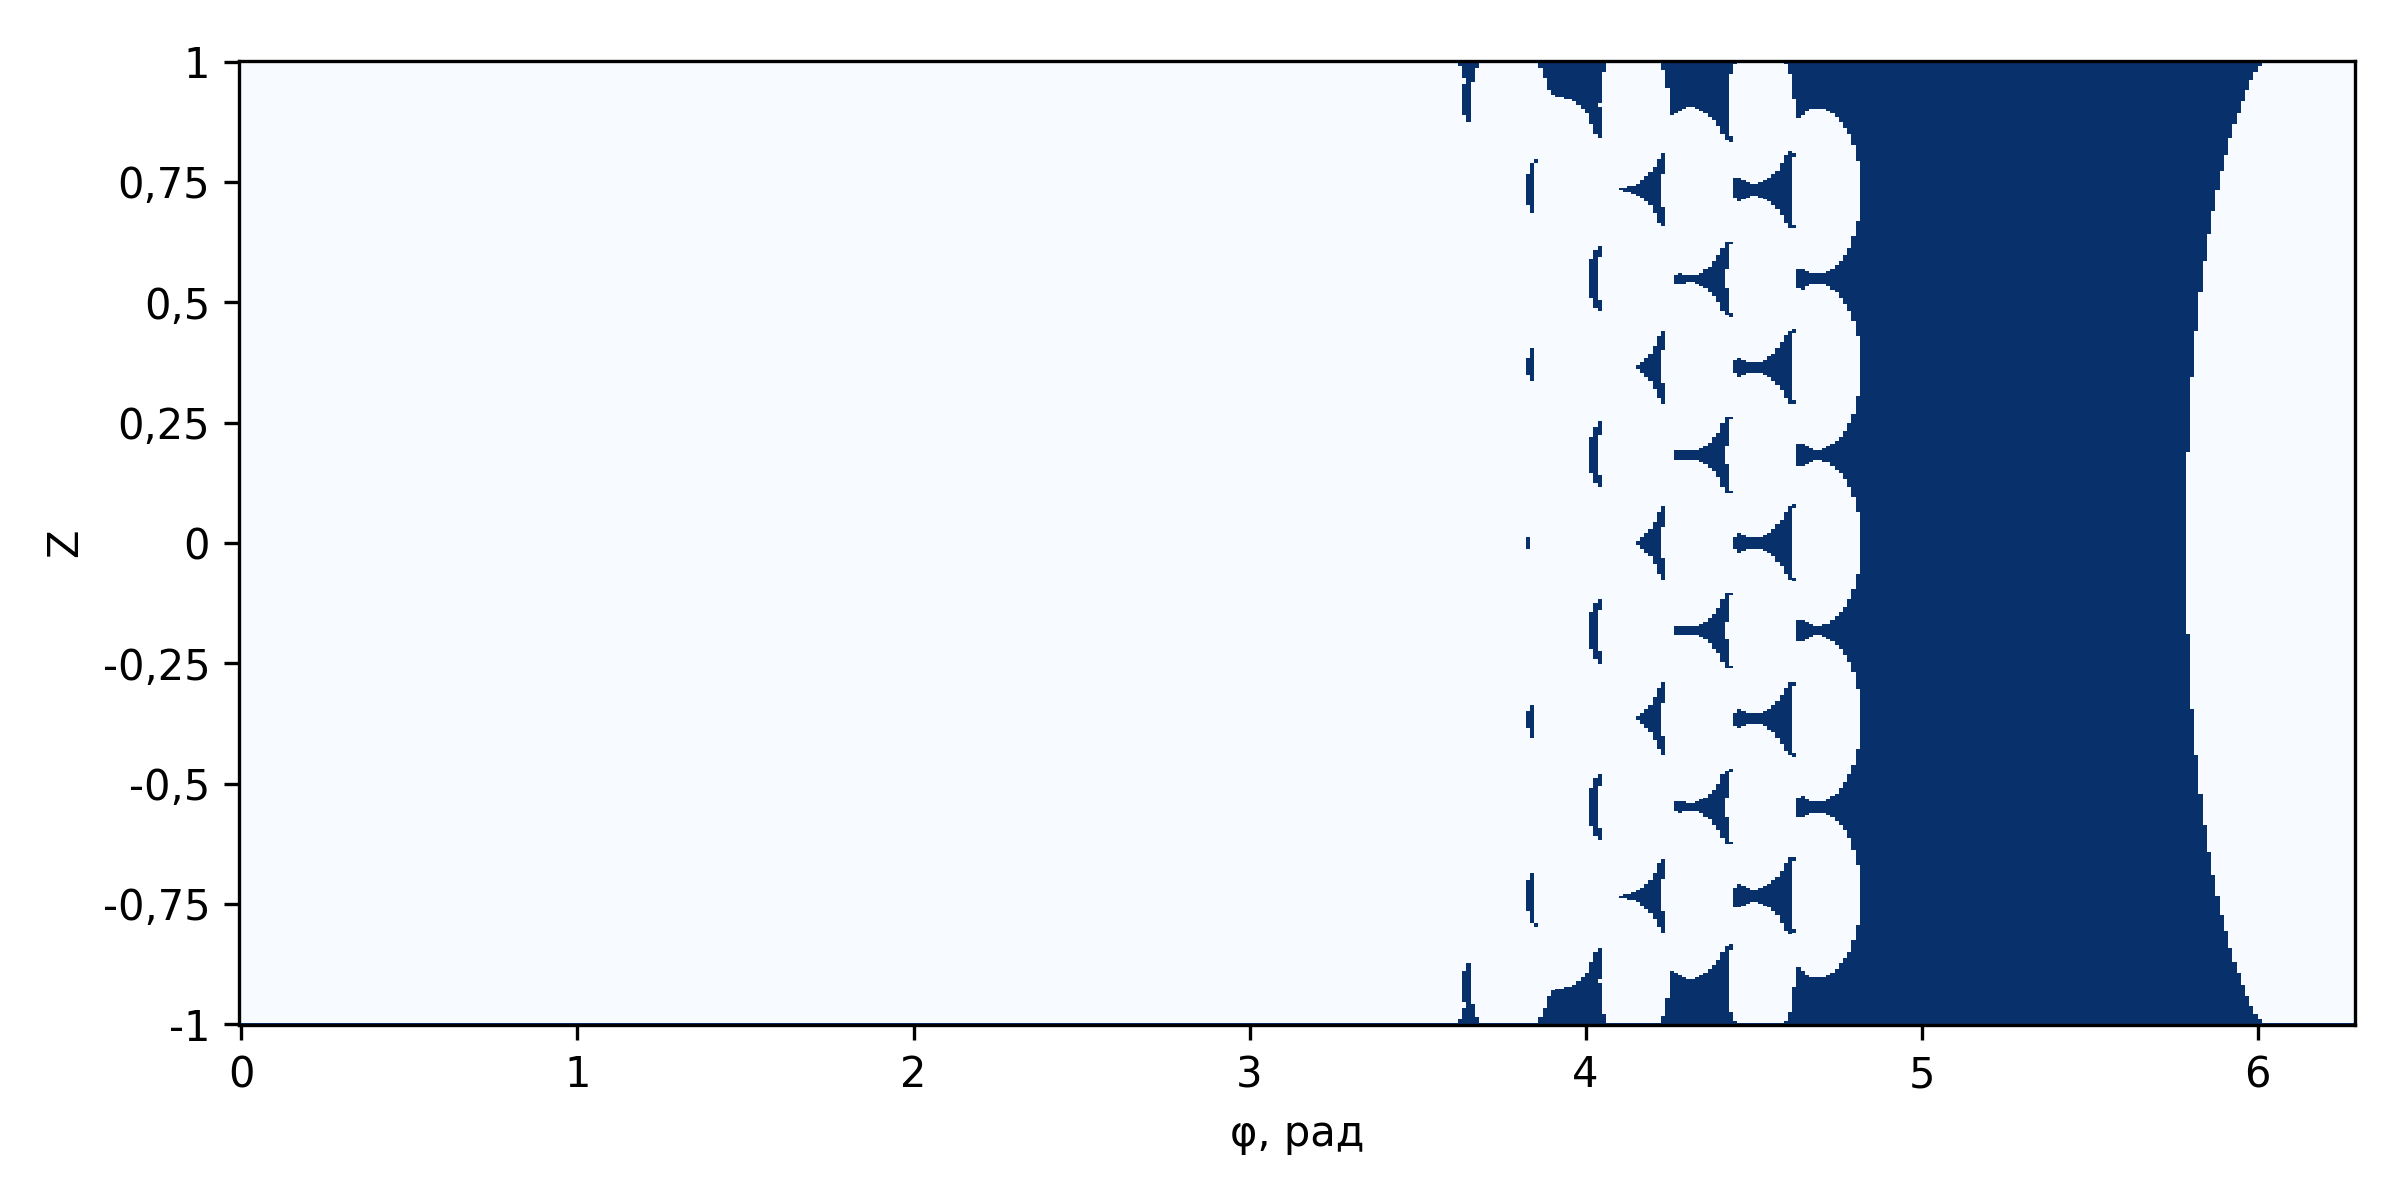
\includegraphics[width=0.75\textwidth]{figures/ch05/fig_5_11.png}
\caption{Карта кавитационной зоны для конфигурации~T2
  ($H_p = 0{,}40$, зона $90^{\circ}$--$270^{\circ}$)
  при $\varepsilon = 0{,}6$.}
\label{fig:cav_T2}
\end{figure}

\begin{figure}[!ht]
\centering
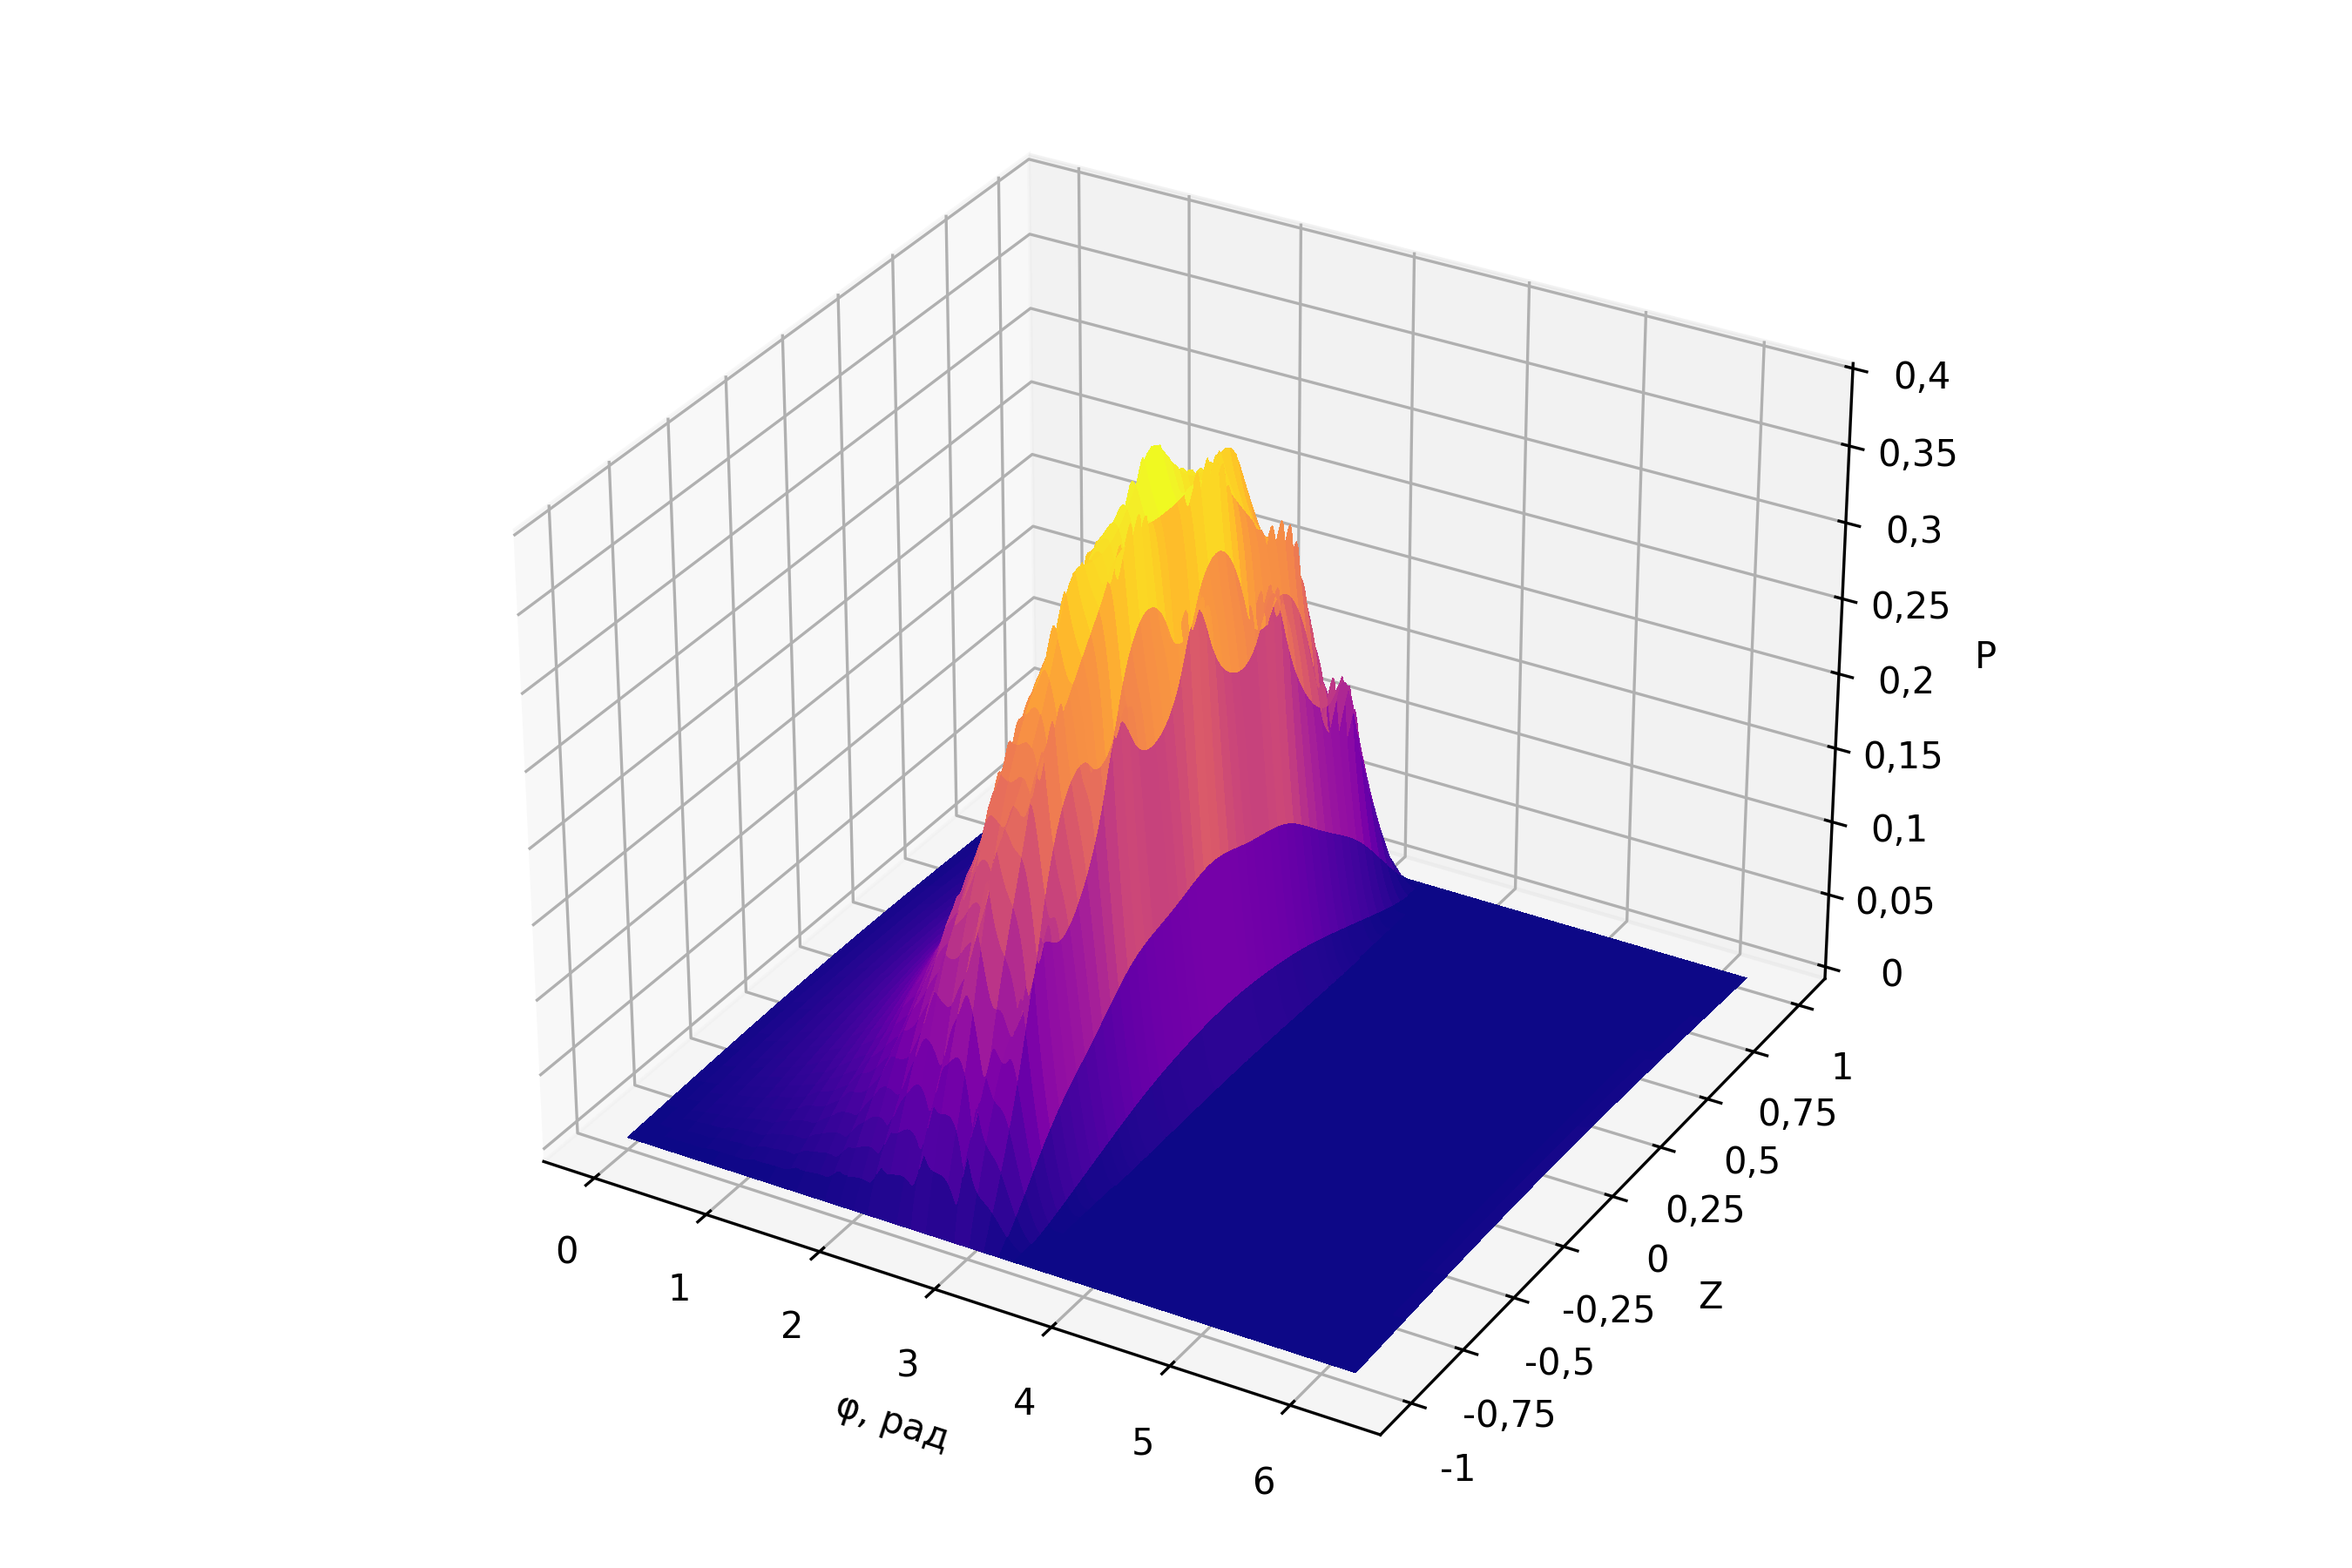
\includegraphics[width=0.75\textwidth]{figures/ch05/fig_5_12.png}
\caption{Поле давления $P(\theta, Z)$ для конфигурации~T3
  ($H_p = 0{,}20$, зона $0^{\circ}$--$180^{\circ}$)
  при $\varepsilon = 0{,}6$. Перенос текстурированной зоны
  в область сходящегося клина изменяет характер локальных возмущений.}
\label{fig:P3D_T3}
\end{figure}

\begin{figure}[!ht]
\centering
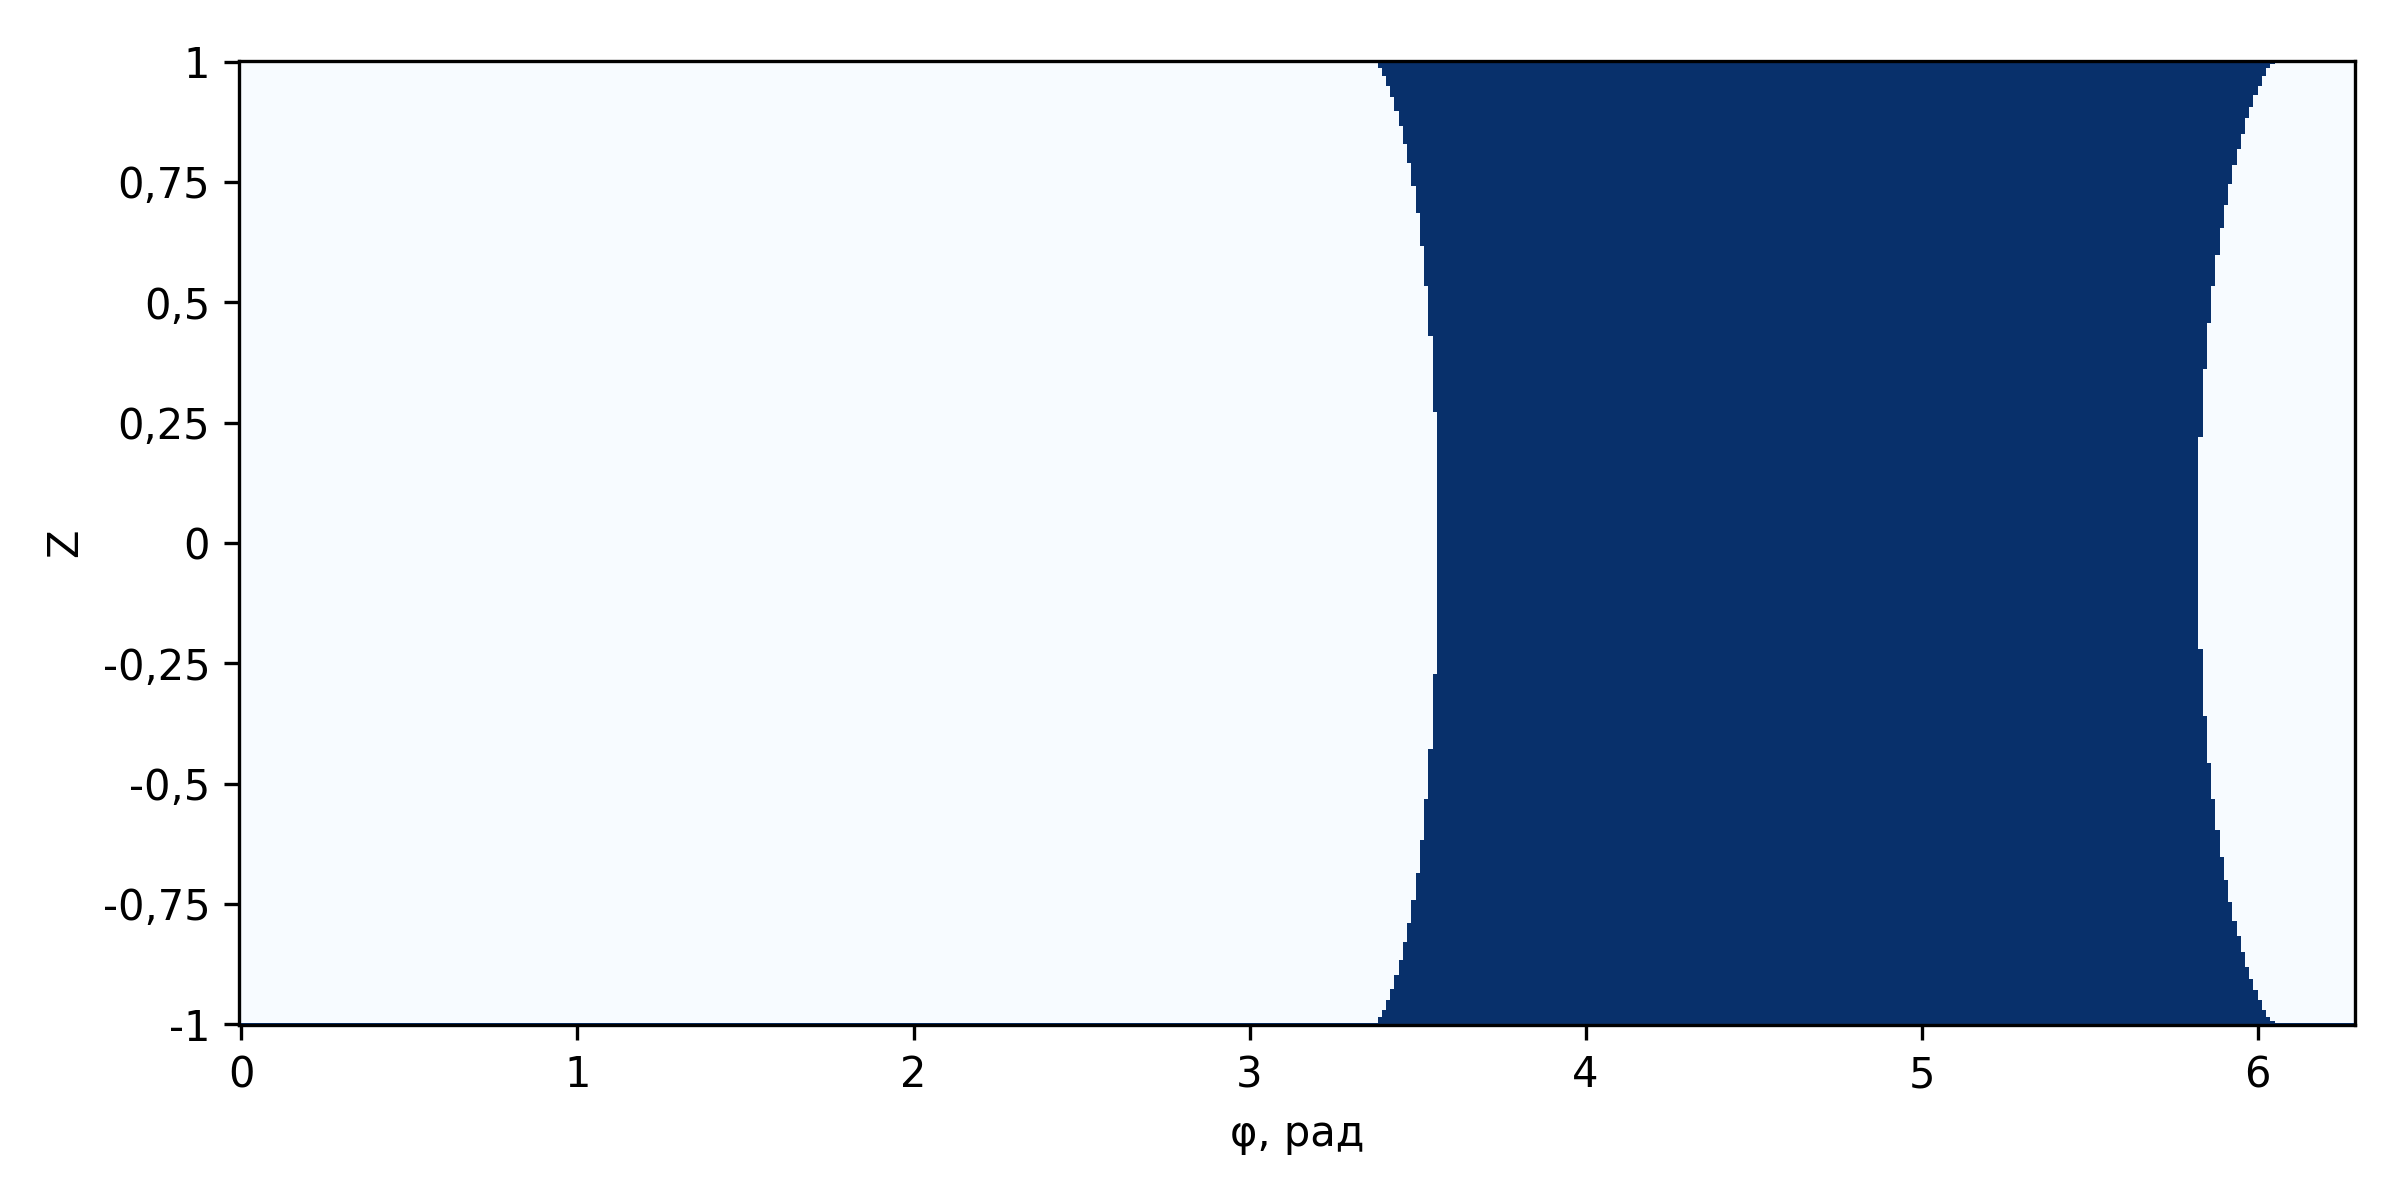
\includegraphics[width=0.75\textwidth]{figures/ch05/fig_5_13.png}
\caption{Карта кавитационной зоны для конфигурации~T3
  ($H_p = 0{,}20$, зона $0^{\circ}$--$180^{\circ}$)
  при $\varepsilon = 0{,}6$.}
\label{fig:cav_T3}
\end{figure}

\FloatBarrier

\textit{Распределение давления в среднем сечении.}
Для более детального анализа на рисунке~\ref{fig:comparison_curves}
представлено распределение давления $P(\theta)$ при $Z = 0$
для гладкого подшипника и конфигурации~T1.

\begin{figure}[!ht]
\centering
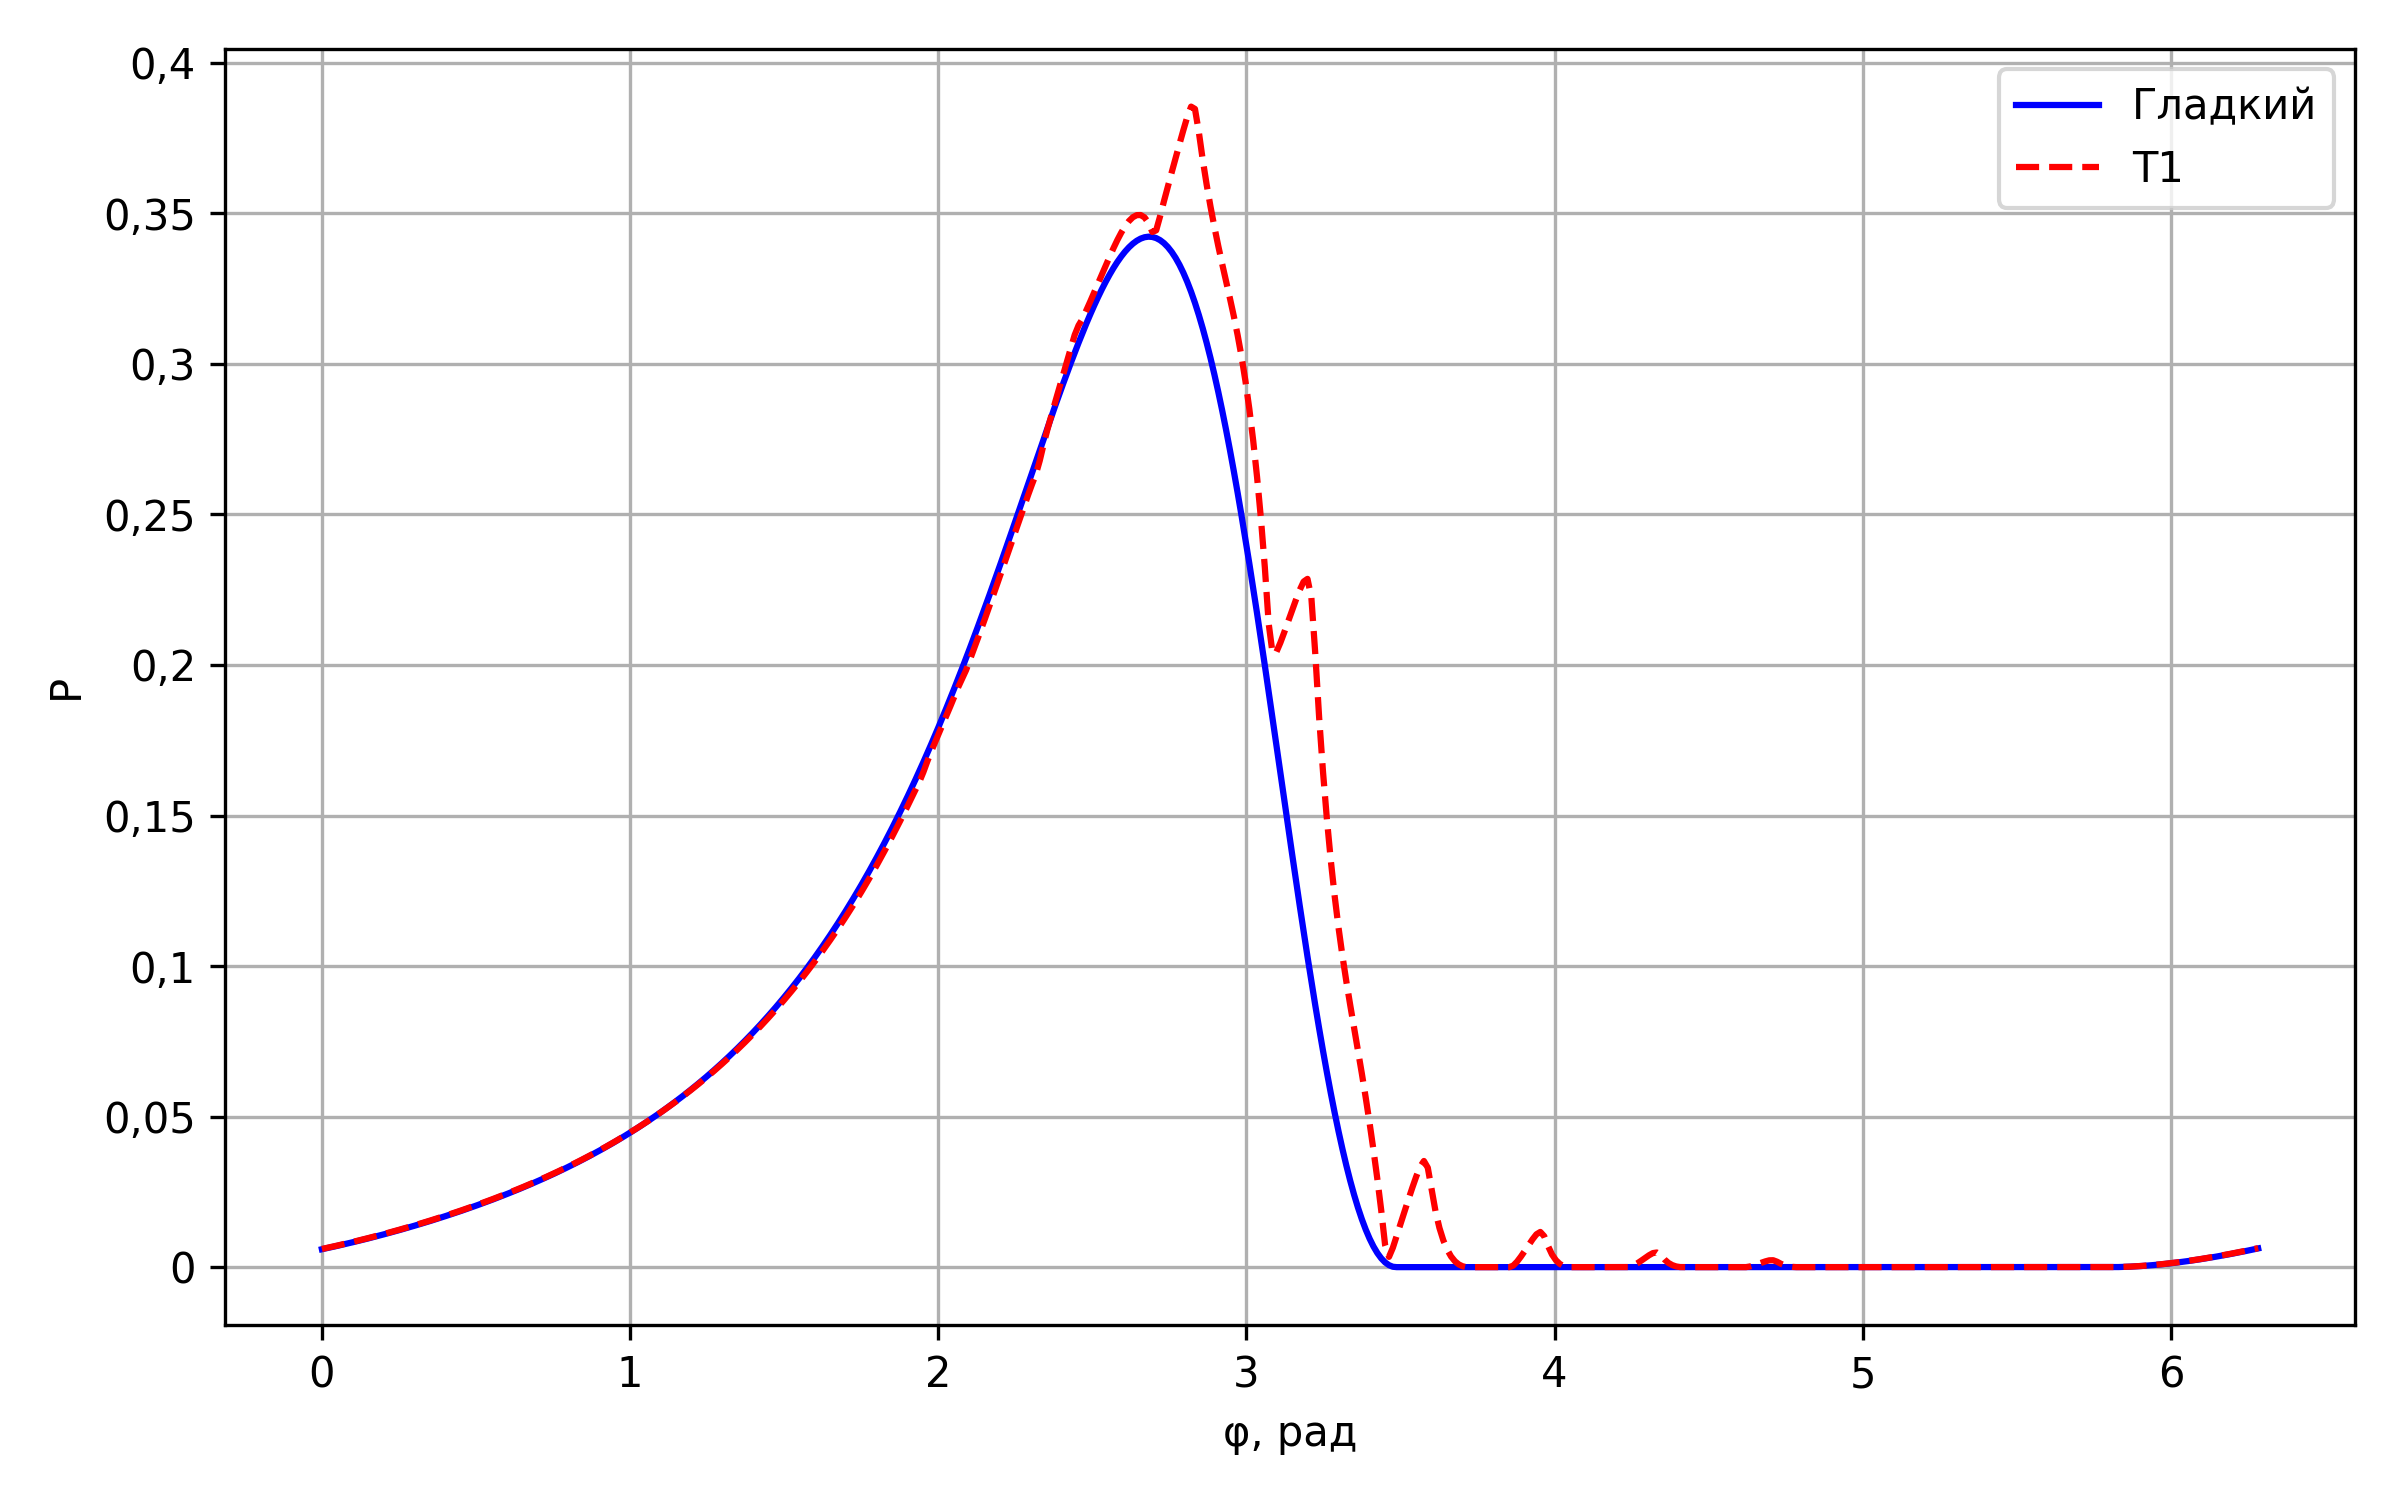
\includegraphics[width=0.75\textwidth]{figures/ch05/fig_5_14.png}
\caption{Распределение безразмерного давления $P(\theta)$ при $Z = 0$
  для гладкого подшипника и конфигурации~T1 ($\varepsilon = 0{,}6$).
  Вторичные пики на кривой T1 соответствуют лункам,
  расположенным в зоне $90^{\circ}$--$270^{\circ}$.}
\label{fig:comparison_curves}
\end{figure}

\begin{figure}[!ht]
\centering
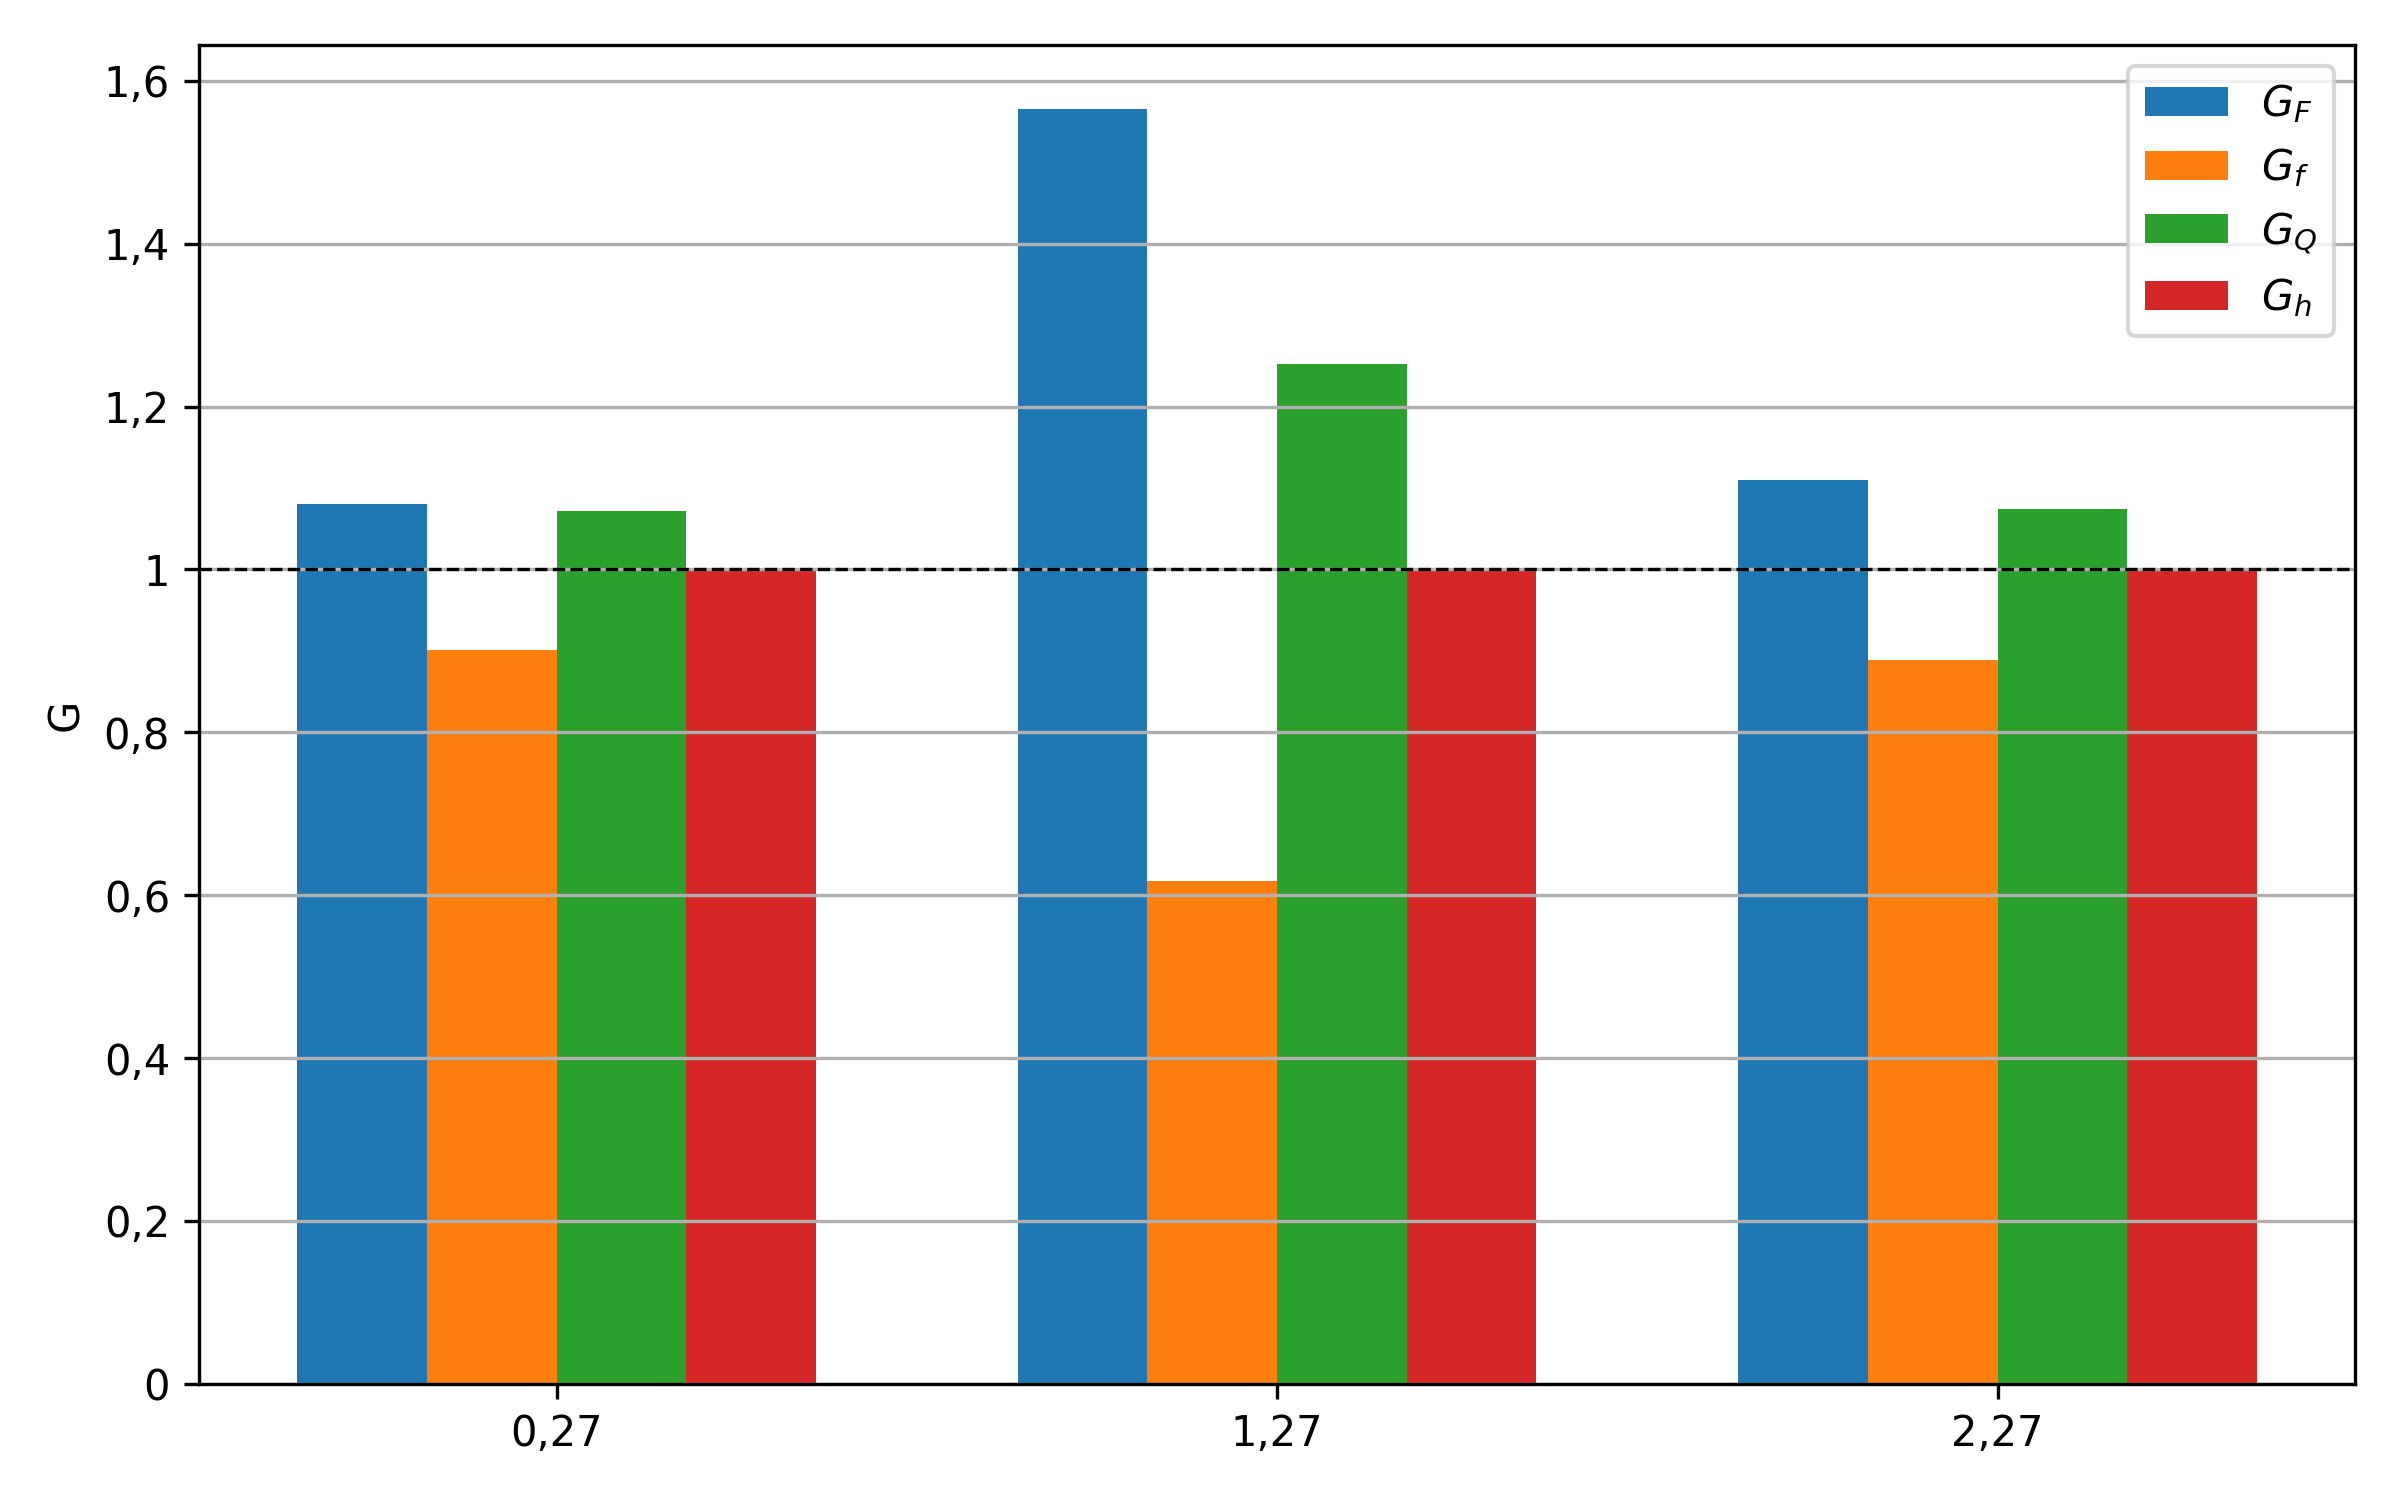
\includegraphics[width=0.75\textwidth]{figures/ch05/fig_5_15.png}
\caption{Нормированные показатели эффективности текстурирования $G_F$, $G_f$,
  $G_Q$, $G_h$ для конфигураций T1, T2, T3 при $\varepsilon = 0{,}6$.
  Пунктирная горизонталь $G = 1$ соответствует уровню гладкого подшипника.}
\label{fig:gains_nom}
\end{figure}

\FloatBarrier

\textit{Нагрузочные характеристики.}
Зависимости несущей способности~$F(\varepsilon)$
и коэффициента трения~$\mu_f(\varepsilon)$ для гладкого
и текстурированного подшипников позволяют оценить эффективность
текстурирования во всём диапазоне рабочих эксцентриситетов.
При малых эксцентриситетах ($\varepsilon \ll 1$), когда зазор
близок к равномерному, влияние микроструктур наиболее выражено:
каждая лунка вносит вклад, сопоставимый с макроскопическим
клиновым эффектом. С ростом~$\varepsilon$ собственный
гидродинамический эффект клинового зазора подшипника усиливается
и начинает доминировать, а относительный вклад текстуры
снижается. Графики нагрузочных характеристик для всех вариантов
представлены на рисунках~\ref{fig:F_vs_epsilon},
\ref{fig:mu_vs_epsilon}, \ref{fig:Q_vs_epsilon}.


\FloatBarrier
\section*{Выводы по главе~5}
\phantomsection\addcontentsline{toc}{section}{Выводы по главе~5}

Проведён статический анализ радиального подшипника скольжения
центробежного насоса в изотермическом приближении с учётом
кавитации по условию Рейнольдса ($P \geq 0$).

Для гладкого подшипника получены поля давления и установлены
границы кавитационной зоны при различных значениях
эксцентриситета. Зависимости несущей
способности~$F(\varepsilon)$, коэффициента
трения~$\mu_f(\varepsilon)$ и осевых
утечек~$Q_{\mathrm{out}}(\varepsilon)$ демонстрируют
характерное поведение гидродинамического подшипника~\cite{rakhonde2018,manshoor2013,madhusudhanarao2020}: рост
несущей способности и убывание коэффициента трения
с увеличением~$\varepsilon$, а также возрастание осевых утечек,
обусловленное ростом перепада давления в осевом направлении~\cite{christiansen2017,zhang2015,fernandes2012}.

Текстурирование поверхности вкладыша эллипсоидальными лунками
в шахматной раскладке модифицирует поле давления: в зоне
расположения элементов возникают локальные возмущения давления,
формируемые микроклиновым эффектом каждой лунки. Конфигурация
кавитационной зоны при текстурировании отличается от эталонного
случая гладкого подшипника~\cite{shenoy2010,elsaid2017}.

Сравнение интегральных характеристик по нормированным
показателям~$G_F$, $G_f$, $G_Q$, $G_h$~\eqref{eq:gain_factors}
при $\varepsilon = 0{,}6$ показывает: конфигурация~T2
($H_p = 0{,}40$, зона $90^{\circ}$--$270^{\circ}$) обеспечивает
наибольший прирост несущей способности ($G_F = 1{,}566$)
и снижение трения ($G_f = 0{,}617$); конфигурации~T1
и~T3 ($H_p = 0{,}20$) показывают умеренный эффект
($G_F \approx 1{,}08$--$1{,}11$, $G_f \approx 0{,}89$--$0{,}90$).
Показатель $G_h = 1{,}00$ для всех конфигураций подтверждает,
что минимальный зазор определяется эксцентриситетом, а не
геометрией лунок.

Эффективность текстурирования существенно зависит от глубины
элементов~$H_p$; влияние зоны нанесения при умеренной глубине
($H_p = 0{,}20$) выражено слабо. Глубина элементов
и коэффициент покрытия~$\varphi$ должны быть согласованы
с рабочим диапазоном эксцентриситетов.

При больших эксцентриситетах ($\varepsilon \to 1$) влияние
микроструктур ослабевает, поскольку макроскопический клиновой
эффект доминирует; в этом режиме текстурирование оказывается
нейтральным или малоэффективным.

Анализ радиального подшипника для иного класса объектов~--
опоры шарошечного долота~-- выполнен в главе~6. Упорный
подшипник рассмотрен в главе~7. Влияние микроструктур
на динамические характеристики подшипника (коэффициенты
жёсткости и демпфирования, устойчивость ротора) составляет
предмет главы~8.



\section{Пример анализа радиального подшипника шарошечного долота}

Второй пример посвящён расчёту радиального подшипника скольжения опоры шарошечного долота. В~отличие от~предыдущего примера, данный подшипник работает при~существенно меньшей скорости скольжения и~более высокой удельной нагрузке, что~обуславливает иной характер результатов и~выводов. Пример иллюстрирует, как~текстурирование поверхности может существенно повысить несущую способность подшипника в~тяжёлых условиях эксплуатации.

% =============================================================
% 6 Анализ радиального подшипника шарошечного долота
% =============================================================
\chapter{Анализ рельефного радиального подшипника шарошечного долота}

\section{Объект исследования и исходные данные}

Объектом исследования в настоящей главе является радиальный
подшипник скольжения опоры шарошки трёхшарошечного долота~\cite{bashmur2024a,bashmur2024b}.
Цапфа (лапа долота) неподвижна относительно корпуса; шарошка
вращается вокруг цапфы. Подшипниковый узел воспринимает
радиальные нагрузки от долота и обеспечивает смазку при тяжёлых
условиях эксплуатации: высокие нагрузки, низкая скорость
скольжения, ограниченная подача смазки.

В отличие от подшипника насоса (глава~5), опора шарошечного долота
работает при скорости скольжения~$U_{\mathrm{eq}}$, примерно
в~90 раз меньшей, и нагрузке $F_{\mathrm{ext}} = 6\,000$~Н на цапфу. Вследствие малой
скорости гидродинамическое давление невелико, и подшипник
функционирует в смешанном или граничном режиме смазки. Применение
детерминированных микроструктур рабочей поверхности направлено
на повышение гидродинамической составляющей несущей способности
и улучшение условий смазки~\cite{bashmur2022,bashmur2023a,bashmur2023b,guo2005}.

Кинематика узла определяется вращением шарошки. Угловая скорость
вращения долота (корпуса):
\begin{equation}
  \omega = \frac{2\pi n}{60},
  \label{eq:bit_omega}
\end{equation}
где $n$~-- частота вращения долота, об/мин. Относительная угловая
скорость шарошки относительно цапфы:
\begin{equation}
  \omega_{\mathrm{rel}} = \omega
    \left(\frac{R_b}{R_k} - 1\right),
  \label{eq:bit_omega_rel}
\end{equation}
где $R_b$~-- радиус долота, $R_k$~-- радиус шарошки.
Эквивалентная скорость скольжения на поверхности цапфы:
\begin{equation}
  U_{\mathrm{eq}} = |\omega_{\mathrm{rel}}|\, R,
  \label{eq:bit_Ueq}
\end{equation}
где $R$~-- радиус цапфы. Подстановка числовых значений даёт
$U_{\mathrm{eq}} \approx 0{,}124$~м/с.

Нагрузка на цапфу определяется из осевой нагрузки на долото~$F_a$.
Нагрузка на одну шарошку при равномерном распределении:
\begin{equation}
  F_{\mathrm{cone}} = \frac{F_a}{3}.
  \label{eq:bit_Fcone}
\end{equation}
В расчётах принято $F_a = 150$~кН, что соответствует
$F_{\mathrm{cone}} = 50$~кН.
Радиальная нагрузка на цапфу:
\begin{equation}
  F_{\mathrm{ext}} = k_L \cdot F_{\mathrm{cone}},
  \label{eq:bit_Fext}
\end{equation}
где $k_L = 0{,}12$~-- коэффициент передачи нагрузки на цапфу
(инженерное оценочное допущение; далее принято $k_L = 0{,}12$).

Основные параметры подшипника сведены в таблицу~\ref{tab:bit_params}.

\begin{table}[!ht]
\centering
\caption{Параметры радиального подшипника скольжения опоры шарошки}
\label{tab:bit_params}
\begin{tabularx}{\textwidth}{|X|c|c|c|}
\hline
\multicolumn{1}{|c|}{\textbf{Параметр}} & \textbf{Обозначение} & \textbf{Значение} & \textbf{Единица} \\
\hline
Радиус цапфы              & $R$              & 30{,}0  & мм \\
\hline
Длина подшипника          & $L$              & 40{,}0  & мм \\
\hline
Радиальный зазор          & $c$              & 60      & мкм \\
\hline
Относительный зазор       & $\psi = c/R$     & $2{,}00 \times 10^{-3}$ & -- \\
\hline
Отношение $L/D$           & $L/D$            & 0{,}667 & -- \\
\hline
Радиус долота             & $R_b$            & 107{,}5 & мм \\
\hline
Радиус шарошки            & $R_k$            & 72{,}0  & мм \\
\hline
Частота вращения          & $n$              & 80      & об/мин \\
\hline
Угловая скорость          & $\omega$         & 8{,}38  & рад/с \\
\hline
Эквивалентная скорость    & $U_{\mathrm{eq}}$ & 0{,}124 & м/с \\
\hline
Динамическая вязкость     & $\mu_0$          & $5{,}5 \times 10^{-2}$ & Па$\cdot$с \\
\hline
Температура               & $T_0$            & 80      & $^{\circ}$C \\
\hline
Суммарная шероховатость   & $\sigma_{\mathrm{eq}}$ & 0{,}89 & мкм \\
\hline
Коэффициент передачи      & $k_L$            & 0{,}12  & -- \\
\hline
Нагрузка на цапфу         & $F_{\mathrm{ext}}$ & 6\,000 & Н \\
\hline
Давление кавитации        & $p_{\mathrm{cav}}$ & 0     & Па \\
\hline
\end{tabularx}
\end{table}

\FloatBarrier

Схема опоры шарошки представлена на рисунке~\ref{fig:bit_scheme}.

\begin{figure}[!ht]
\centering
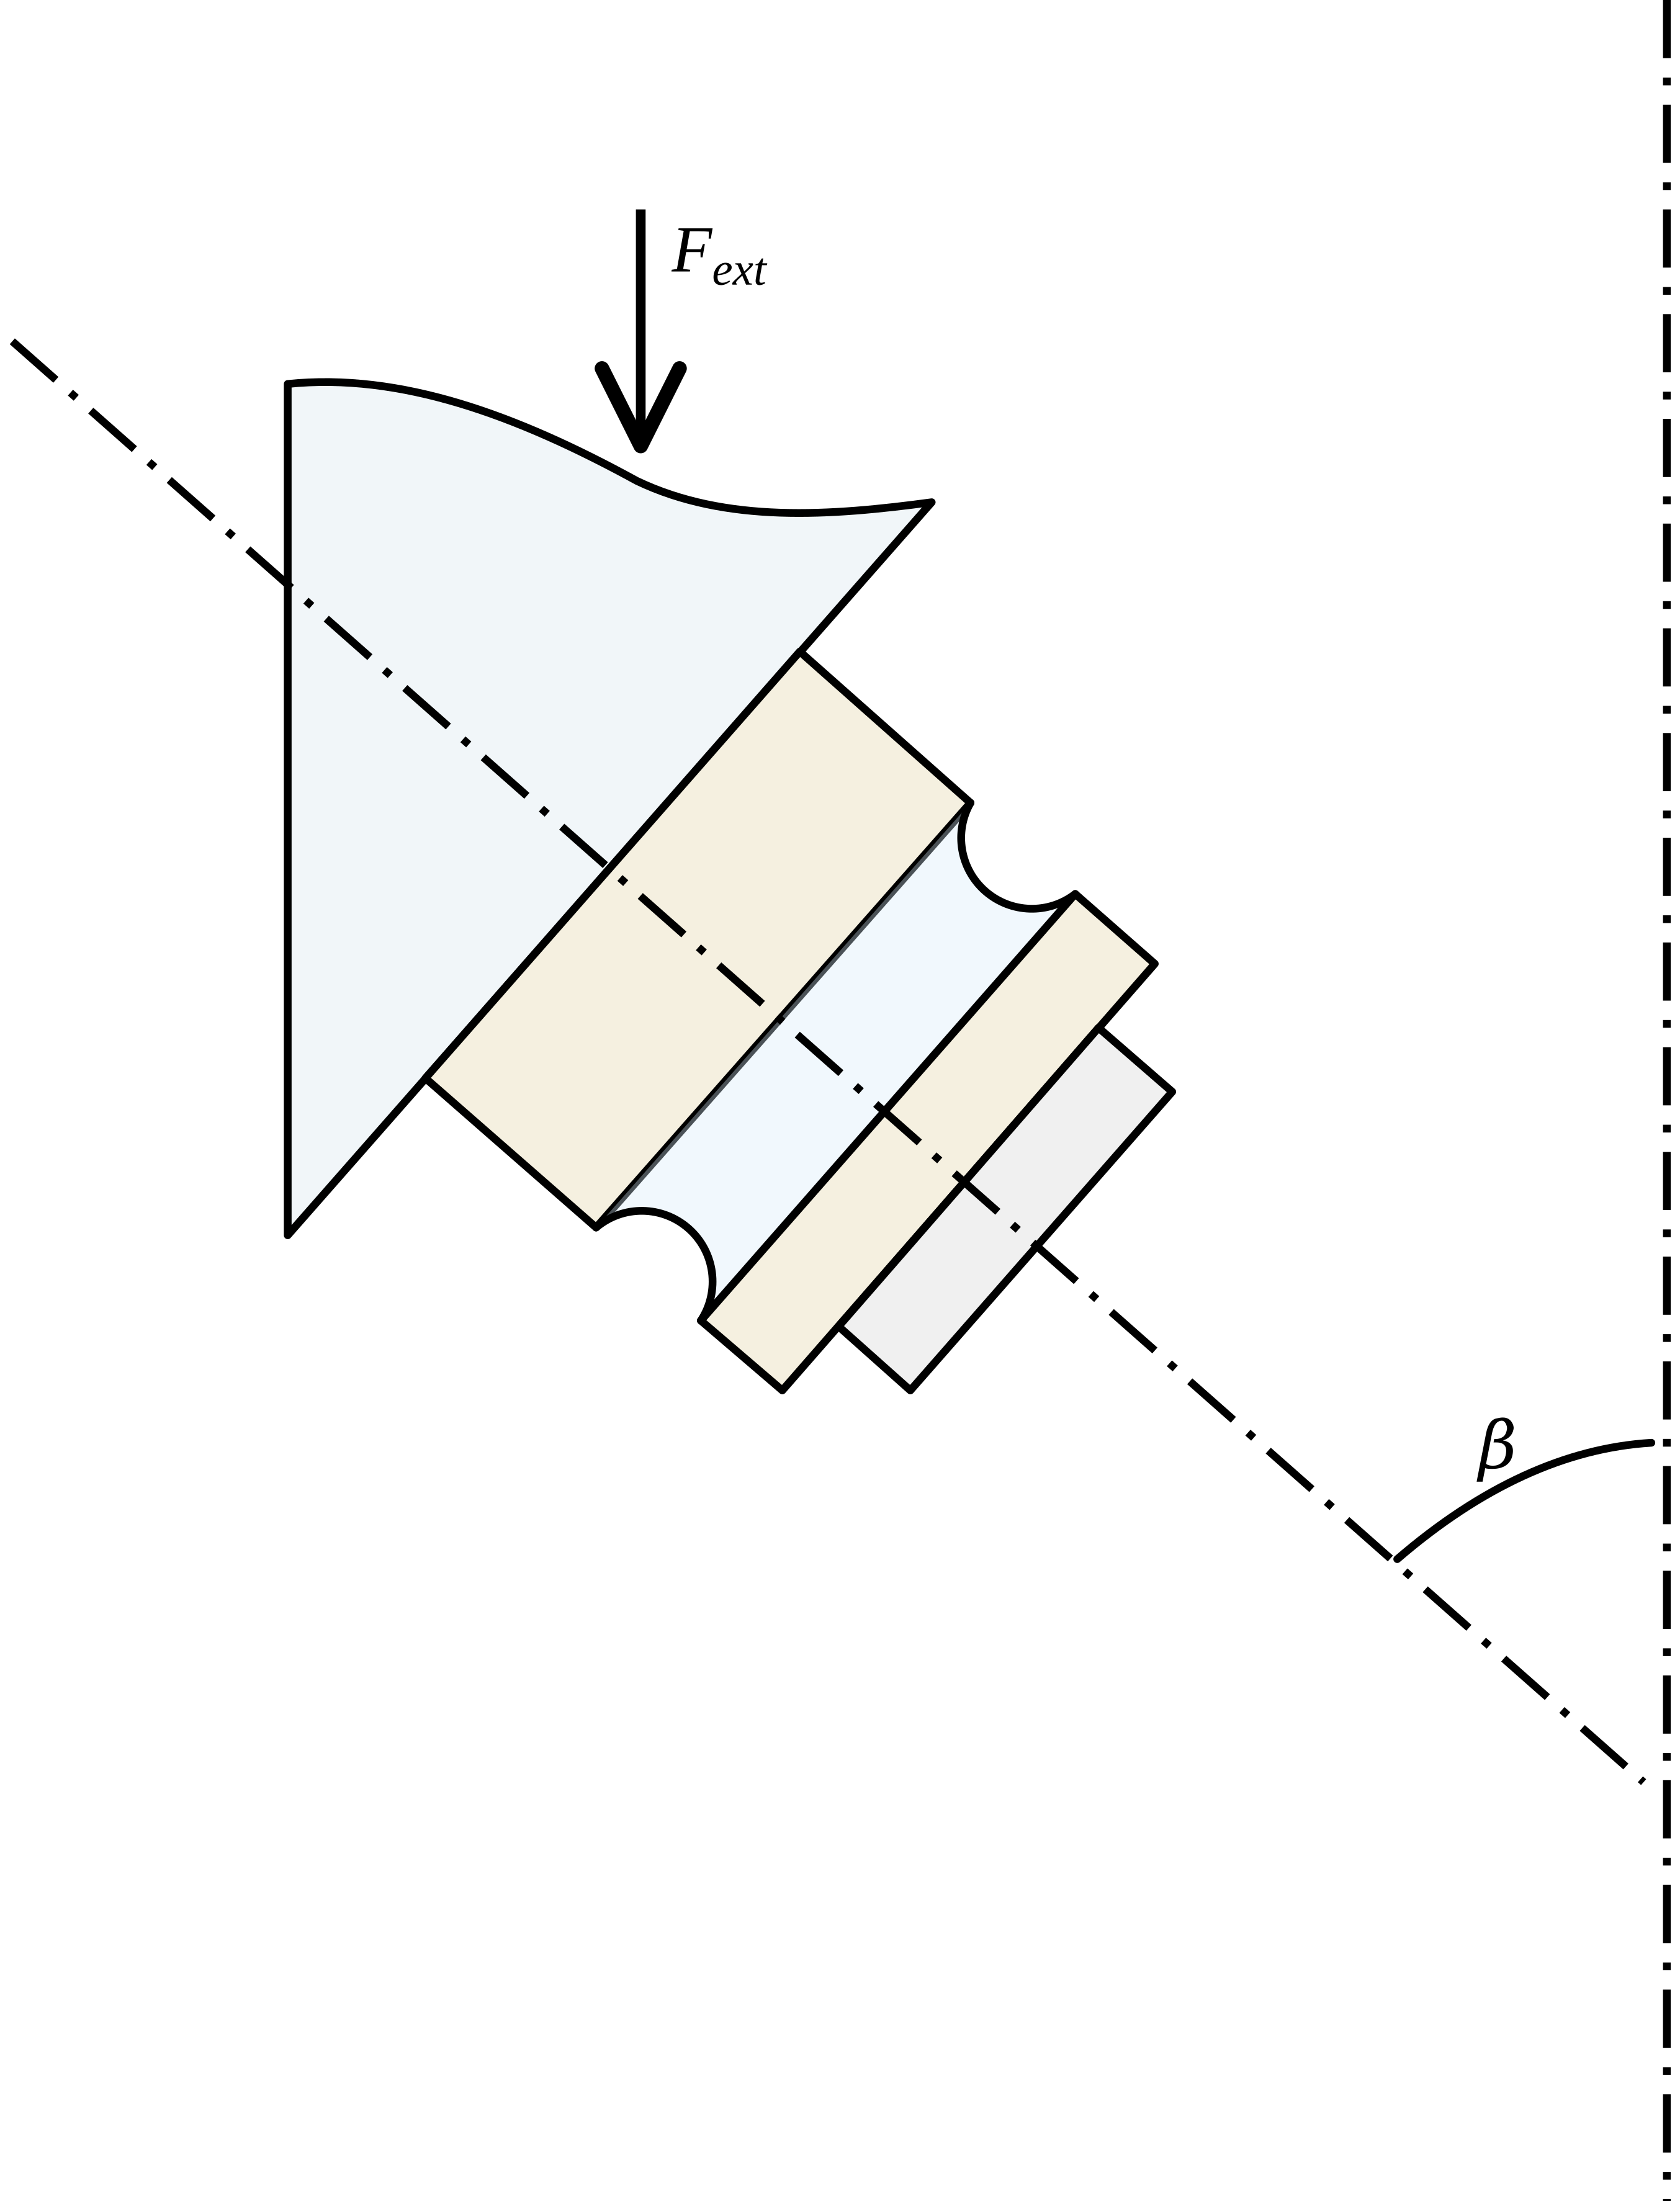
\includegraphics[width=\textwidth,height=0.9\textheight,keepaspectratio]{figures/ch06/fig_6_1.png}
\caption{Схема опоры шарошки трёхшарошечного долота}
\label{fig:bit_scheme}
\end{figure}

\FloatBarrier


\section{Постановка задачи}\label{sec:problem_statement_ch6}

Расчётная область представляет собой развёрнутую поверхность
смазочного зазора $(\theta, z) \in [0,\,2\pi] \times [-L/2,\,L/2]$,
где $\theta$~-- окружная координата, $z$~-- осевая координата.
В тексте главы окружная координата обозначается~$\theta$;
на рисунках ось подписана~$\varphi$; везде $\theta \equiv \varphi$.
При переходе к безразмерным переменным (подраздел~2.1.6)
осевая координата нормируется на полудлину: $Z = 2z/L$,
так что $Z \in [-1,\,1]$.

Для гладкого цилиндрического подшипника безразмерная толщина
зазора определяется законом~\eqref{eq:journal_h_ch5}:
\begin{equation}
  H(\theta) = 1 + \varepsilon\cos\theta,
  \label{eq:bit_h}
\end{equation}
где $\varepsilon = e/c$~-- относительный эксцентриситет
($0 \leq \varepsilon < 1$). Для подшипника с детерминированными
микроструктурами толщина зазора записывается в виде
суперпозиции~\eqref{eq:journal_h_tex_ch5}:
\begin{equation}
  H = H_0(\theta) + \Delta H_t(\theta, Z).
  \label{eq:bit_h_tex}
\end{equation}
где $H_0(\theta) = 1 + \varepsilon\cos\theta$~-- базовый зазор гладкого подшипника~\eqref{eq:bit_h}, $\Delta H_t$~-- добавка микрорельефа (подраздел~2.2).

Распределение давления описывается безразмерным уравнением
Рейнольдса~\eqref{eq:reynolds_nondim} с параметром
анизотропии~$\Lambda$~\eqref{eq:nondim_Lambda}.

Граничные условия: по окружной координате~$\theta$ поле давления
периодично ($P(\theta = 0) = P(\theta = 2\pi)$); на торцах
подшипника давление равно атмосферному ($P = 0$ при $Z = \pm 1$).
Кавитация учитывается по условию Рейнольдса: $P \geq 0$.

В отличие от главы~5, где эксцентриситет задавался как входной
параметр и вычислялась несущая сила~$F(\varepsilon)$, в настоящей
главе рассматривается обратная задача: задаётся внешняя нагрузка
$F_{\mathrm{ext}}$, а равновесный эксцентриситет~$\varepsilon^*$
определяется из условия равновесия:
\begin{equation}
  F(\varepsilon^*) = F_{\mathrm{ext}}.
  \label{eq:bit_equilibrium}
\end{equation}
Решение уравнения~\eqref{eq:bit_equilibrium} выполняется методом
бисекции по~$\varepsilon \in [0{,}05;\; 0{,}97]$ с допуском~$1\,\%$.

Для оценки режима смазки вводится минимальная толщина плёнки:
\begin{equation}
  h_{\min} = c\,(1 - \varepsilon),
  \label{eq:bit_hmin}
\end{equation}
а также параметр плёнки:
\begin{equation}
  \lambda = \frac{h_{\min}}{\sigma_{\mathrm{eq}}},
  \label{eq:bit_lambda}
\end{equation}
где $\sigma_{\mathrm{eq}}$~-- суммарная шероховатость поверхностей.
Классификация режимов смазки по параметру~$\lambda$:
$\lambda < 1$~-- граничный режим;
$1 \leq \lambda \leq 3$~-- смешанный режим;
$\lambda > 3$~-- гидродинамический режим.

Для сравнительной оценки условий работы узла вводится
$PV$-параметр:
\begin{equation}
  p_0 = \frac{F}{2\,R\,L}, \qquad
  PV = p_0 \cdot U_{\mathrm{eq}},
  \label{eq:bit_PV}
\end{equation}
и индекс износа:
\begin{equation}
  I_w = \frac{PV}{h_{\min}}.
  \label{eq:bit_Iw}
\end{equation}
Величина~$I_w$ является суррогатным сравнительным
индексом, характеризующим интенсивность изнашивания; строгое
соответствие закону Арчарда не предполагается.

Допущения, принятые в настоящей главе, включают: изотермическое
приближение ($T = T_0$, $\mu = \mathrm{const}$), постоянство
плотности ($\rho = \mathrm{const}$) и кавитация по условию
Рейнольдса ($P \geq 0$).


\section{Результаты для гладкого подшипника}

При расчётном пределе эксцентриситета $\varepsilon = 0{,}97$
гладкий подшипник развивает несущую силу
$F(\varepsilon = 0{,}97) = 1907$~Н. Это составляет около~$3{,}8\,\%$
от нагрузки на шарошку $F_{\mathrm{cone}} = F_a / 3 = 50\,000$~Н
и менее трети рабочей нагрузки $F_{\mathrm{ext}} = 6\,000$~Н.

Низкая несущая способность обусловлена малой скоростью скольжения
$U_{\mathrm{eq}} \approx 0{,}124$~м/с, примерно в~90 раз меньшей,
чем у подшипника насоса главы~5. Гидродинамическое давление
пропорционально скорости ($p \sim \mu_0\, U_{\mathrm{eq}}\, R / c^2$), поэтому даже
при предельном эксцентриситете несущая сила не достигает
$F_{\mathrm{ext}}$.

При рабочей нагрузке $F_{\mathrm{ext}} = 6\,000$~Н гладкий
подшипник не имеет равновесной рабочей точки в чисто
гидродинамической постановке. Режим смазки~-- смешанный или
граничный. Применение детерминированных микроструктур
рассматривается как средство повышения гидродинамической
составляющей несущей способности.


\section{Выбор и параметры микроструктуры}

В качестве элементов микрорельефа выбраны эллипсоидальные лунки
с профилем~\eqref{eq:profile_ellipsoidal}, расположенные
по шахматной схеме~\eqref{eq:layout_staggered}. Выбор типа
элемента и раскладки аналогичен главе~5 (подраздел~2.2).

Зона нанесения микроструктур определяется расположением области
максимального давления. В радиальном подшипнике максимум давления
формируется вблизи $\theta \approx \pi$ (зона минимального зазора).
Конфигурации~T1 и~T2 нанесены в секторе
$90^{\circ}$--$270^{\circ}$, включающем эту зону. Конфигурация~T3
нанесена в секторе $0^{\circ}$--$180^{\circ}$ (зона сходящегося
клина).

Параметры микроструктур (безразмерные полуоси~$A^*$, $B^*$)
пересчитаны под геометрию опоры шарошки ($R = 30$~мм,
$L = 40$~мм); числовые значения отличаются от конфигураций
главы~5 ($R = 35$~мм, $L = 56$~мм). Поэтому сравнение текстур
выполняется только внутри настоящей главы; прямое количественное
сопоставление с главой~5 не проводится.

Параметры рассматриваемых конфигураций приведены в
таблице~\ref{tab:bit_texture_configs}.

\begin{table}[!ht]
\centering
\caption{Параметры конфигураций текстуры для подшипника шарошечного долота}
\label{tab:bit_texture_configs}
\begin{tabularx}{\textwidth}{|X|c|c|c|c|}
\hline
\multicolumn{1}{|c|}{\textbf{Конфигурация}} & $\boldsymbol{H_p}$ & $\boldsymbol{A^*}$ & $\boldsymbol{B^*}$ & \textbf{Зона нанесения} \\
\hline
T1 & 0{,}20 & 0{,}0600 & 0{,}0367 & $90^{\circ}$--$270^{\circ}$ \\
\hline
T2 & 0{,}40 & 0{,}0600 & 0{,}0367 & $90^{\circ}$--$270^{\circ}$ \\
\hline
T3 & 0{,}20 & 0{,}0600 & 0{,}0367 & $0^{\circ}$--$180^{\circ}$ \\
\hline
\end{tabularx}
\end{table}


\section{Сравнение гладкого и текстурированного подшипников}

\textit{Рабочие точки при заданной нагрузке на цапфу.}
Все три конфигурации текстуры (T1--T3) обеспечивают равновесную
рабочую точку при $F_{\mathrm{ext}} = 6\,000$~Н; гладкий
подшипник рабочей точки не имеет. Результаты расчёта рабочих точек
сведены в таблицу~\ref{tab:bit_results}.

\begin{table}[!ht]
\centering
\caption{Характеристики подшипника в рабочей точке
  при $F_{\mathrm{ext}} = 6\,000$~Н}
\label{tab:bit_results}
\resizebox{\textwidth}{!}{%
\begin{tabular}{|l|c|c|c|c|c|c|c|c|}
\hline
\multicolumn{1}{|c|}{\textbf{Вар.}}
  & $\boldsymbol{\varepsilon}$
  & $\boldsymbol{F}$, Н
  & $\boldsymbol{\varphi}$, $^{\circ}$
  & $\boldsymbol{\mu_f}$
  & $\boldsymbol{h_{\min}}$, мкм
  & $\boldsymbol{\lambda}$
  & $\boldsymbol{PV}$, Па$\cdot$м/с
  & $\boldsymbol{I_w}$ \\
\hline
T1 & 0{,}966 & 6004 & 175{,}4 & 0{,}00123 & 2{,}04 & 2{,}28
   & 309\,981 & $1{,}5 \cdot 10^{11}$ \\
\hline
T2 & 0{,}956 & 6044 & 175{,}9 & 0{,}00107 & 2{,}66 & 2{,}98
   & 312\,090 & $1{,}2 \cdot 10^{11}$ \\
\hline
T3 & 0{,}969 & 5956 & 173{,}8 & 0{,}00136 & 1{,}85 & 2{,}07
   & 307\,503 & $1{,}7 \cdot 10^{11}$ \\
\hline
\end{tabular}%
}
\end{table}

\FloatBarrier

Все три конфигурации работают в смешанном режиме смазки
($1 \leq \lambda \leq 3$).

Приведённый коэффициент трения~$\mu_f$ соответствует
гидродинамической составляющей модели. В смешанном режиме
($\lambda < 3$) реальное трение в узле выше вследствие
дополнительного вклада контактного взаимодействия шероховатостей
поверхностей.

Конфигурация~T2 демонстрирует наилучшие характеристики:
наименьший эксцентриситет $\varepsilon = 0{,}956$, наибольший
минимальный зазор $h_{\min} = 2{,}66$~мкм, параметр плёнки
$\lambda = 2{,}98$~-- значение, наиболее близкое к границе
гидродинамического режима. Конфигурация~T3, в которой текстура
расположена вне зоны максимального давления, показывает наихудшие
значения~$h_{\min}$ и~$\lambda$.


\textit{Грузоподъёмность при расчётном пределе эксцентриситета.}
При расчётном пределе $\varepsilon = 0{,}97$ несущая сила
составляет: гладкий подшипник~-- $1\,907$~Н; T1~-- $7\,237$~Н;
T2~-- $7\,549$~Н; T3~-- $6\,212$~Н. Максимальная грузоподъёмность
конфигурации~T2 в~$3{,}96$ раза превышает значение гладкого
подшипника. Горизонталь $F_{\mathrm{ext}} = 6\,000$~Н пересекает
кривые~T1, T2, T3, но не кривую гладкого подшипника: рабочая точка
при заданной нагрузке существует только при наличии текстуры.

Зависимости несущей силы~$F(\varepsilon)$ для всех вариантов
представлены на рисунке~\ref{fig:bit_operating_points}.

\begin{figure}[!ht]
\centering
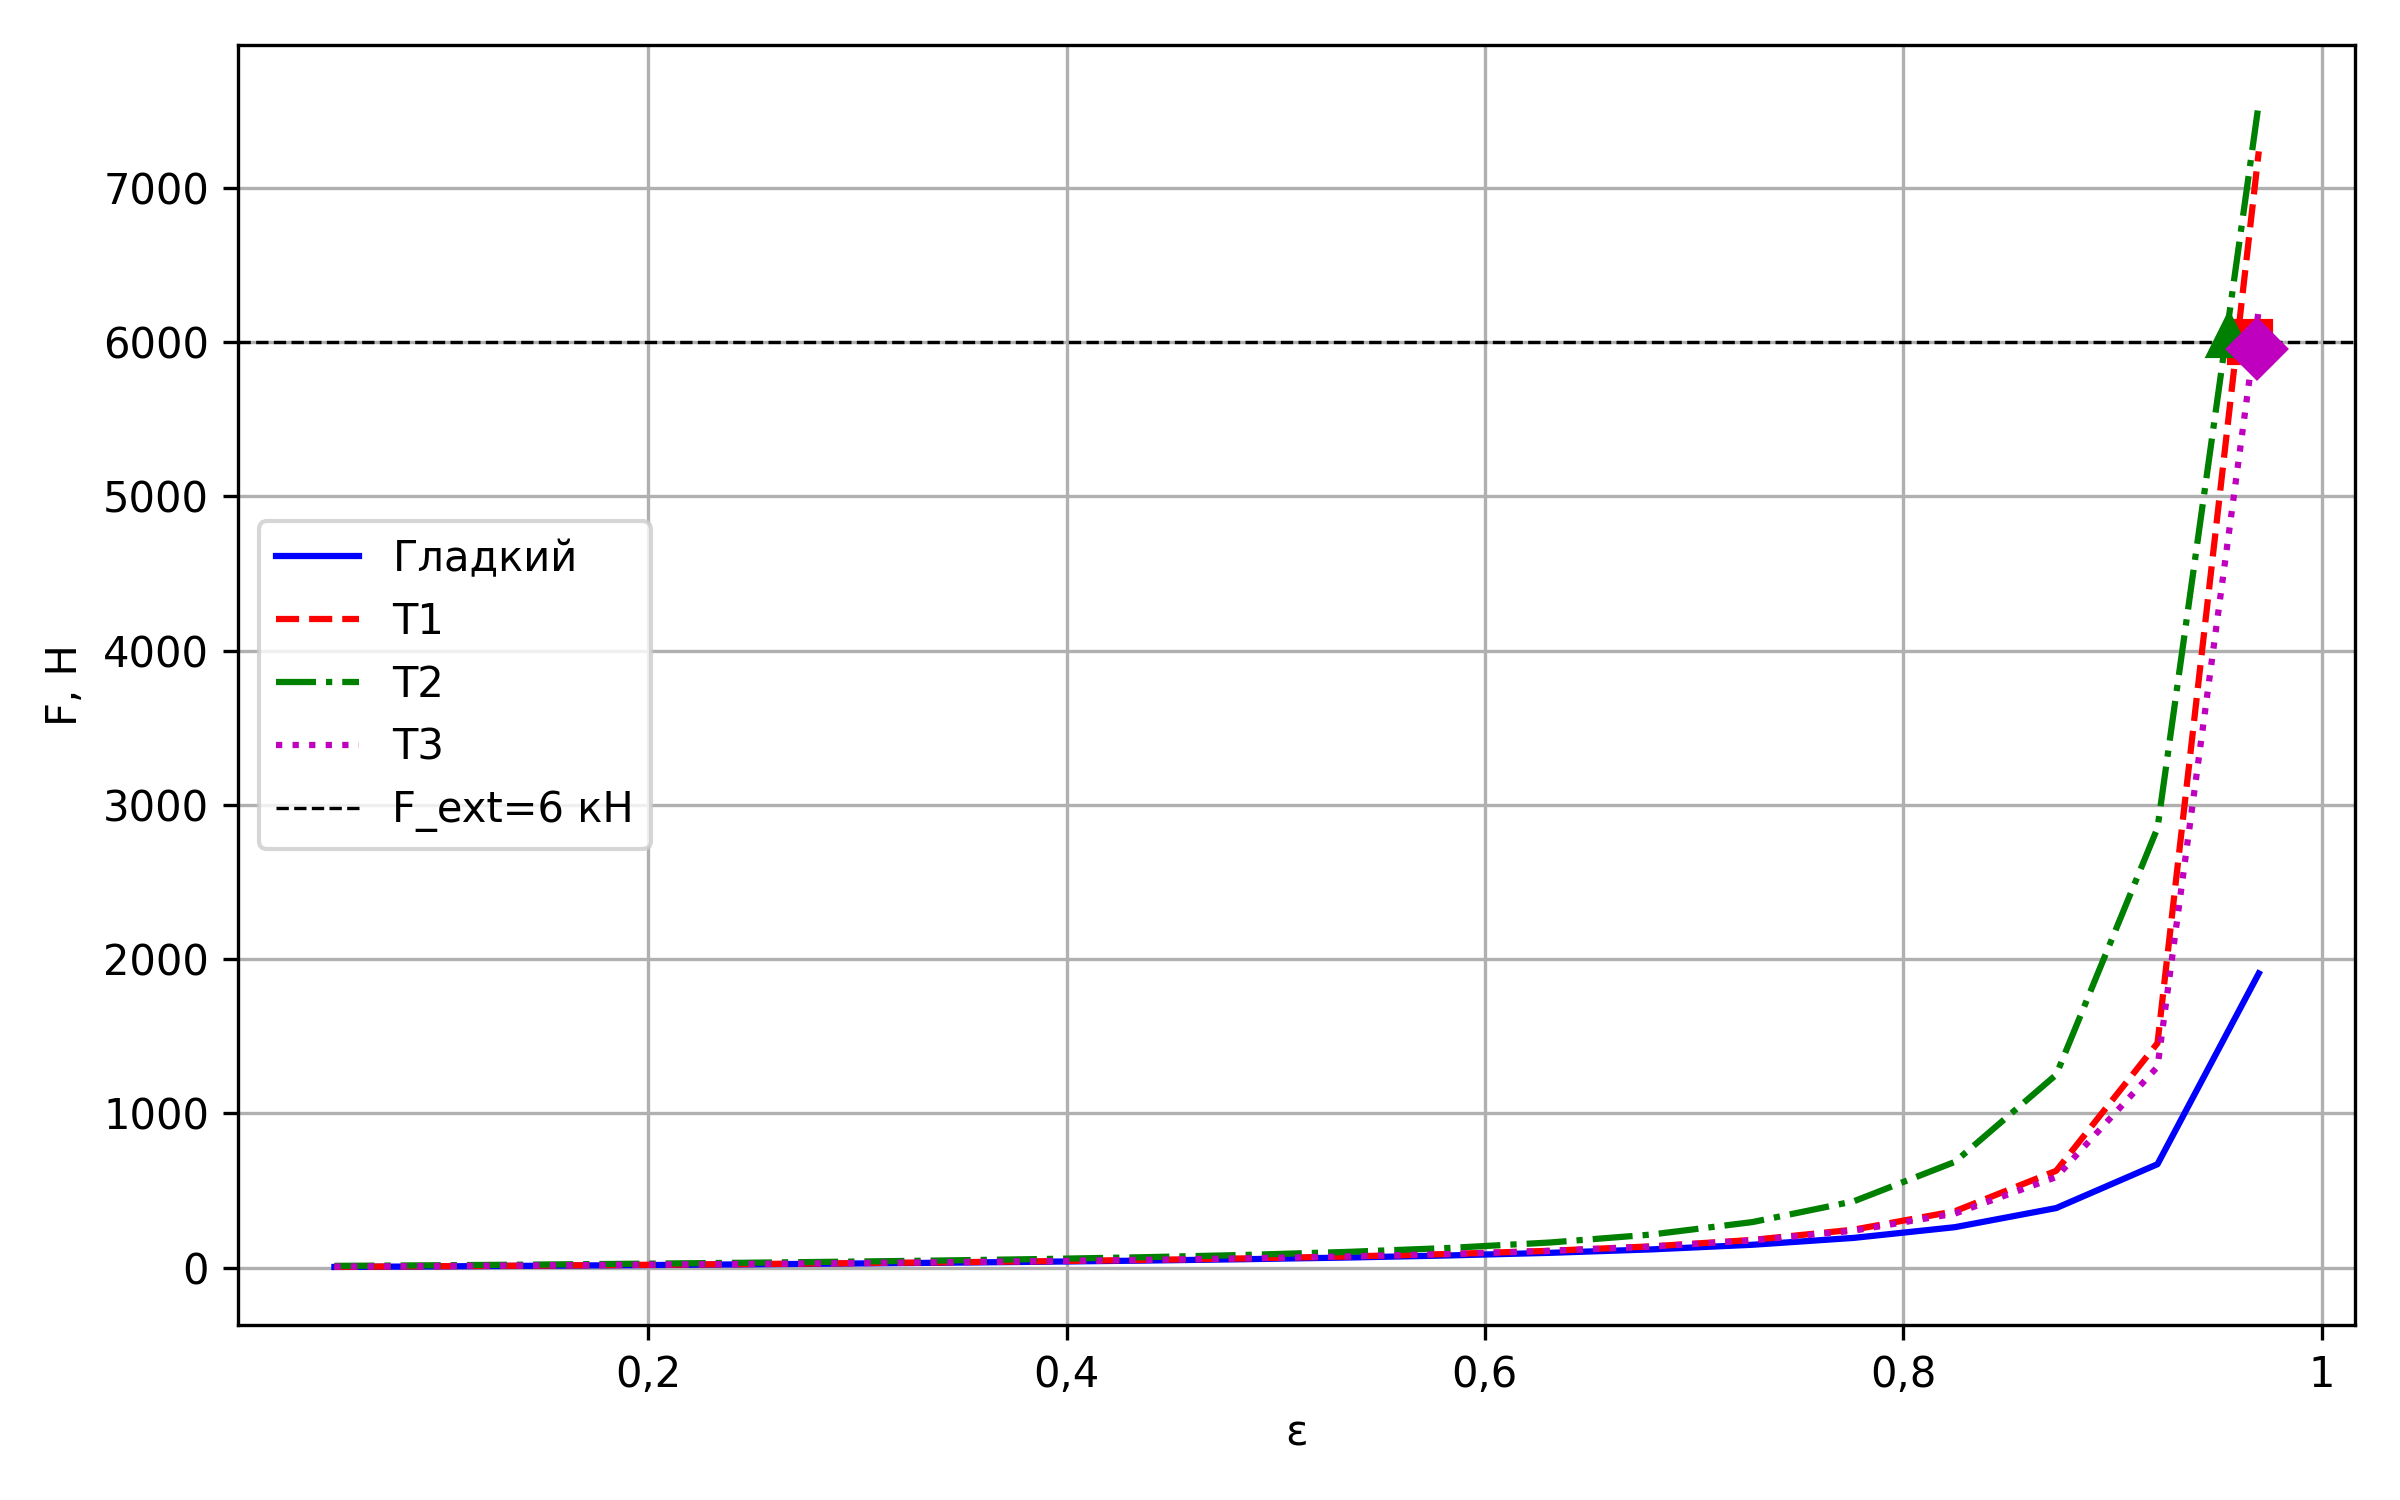
\includegraphics[width=\textwidth,height=0.9\textheight,keepaspectratio]{figures/ch06/fig_6_2.png}
\caption{Зависимость несущей силы $F$ от эксцентриситета $\varepsilon$
  для гладкого подшипника и конфигураций T1, T2, T3.
  Пунктирная горизонталь~-- рабочая нагрузка $F_{\mathrm{ext}} = 6\,000$~Н;
  маркеры~-- равновесные рабочие точки текстурированных конфигураций.}
\label{fig:bit_operating_points}
\end{figure}

\FloatBarrier

Параметр плёнки~$\lambda$ в рабочих точках текстурированных
конфигураций представлен на рисунке~\ref{fig:bit_lambda_comparison}.

\begin{figure}[!ht]
\centering
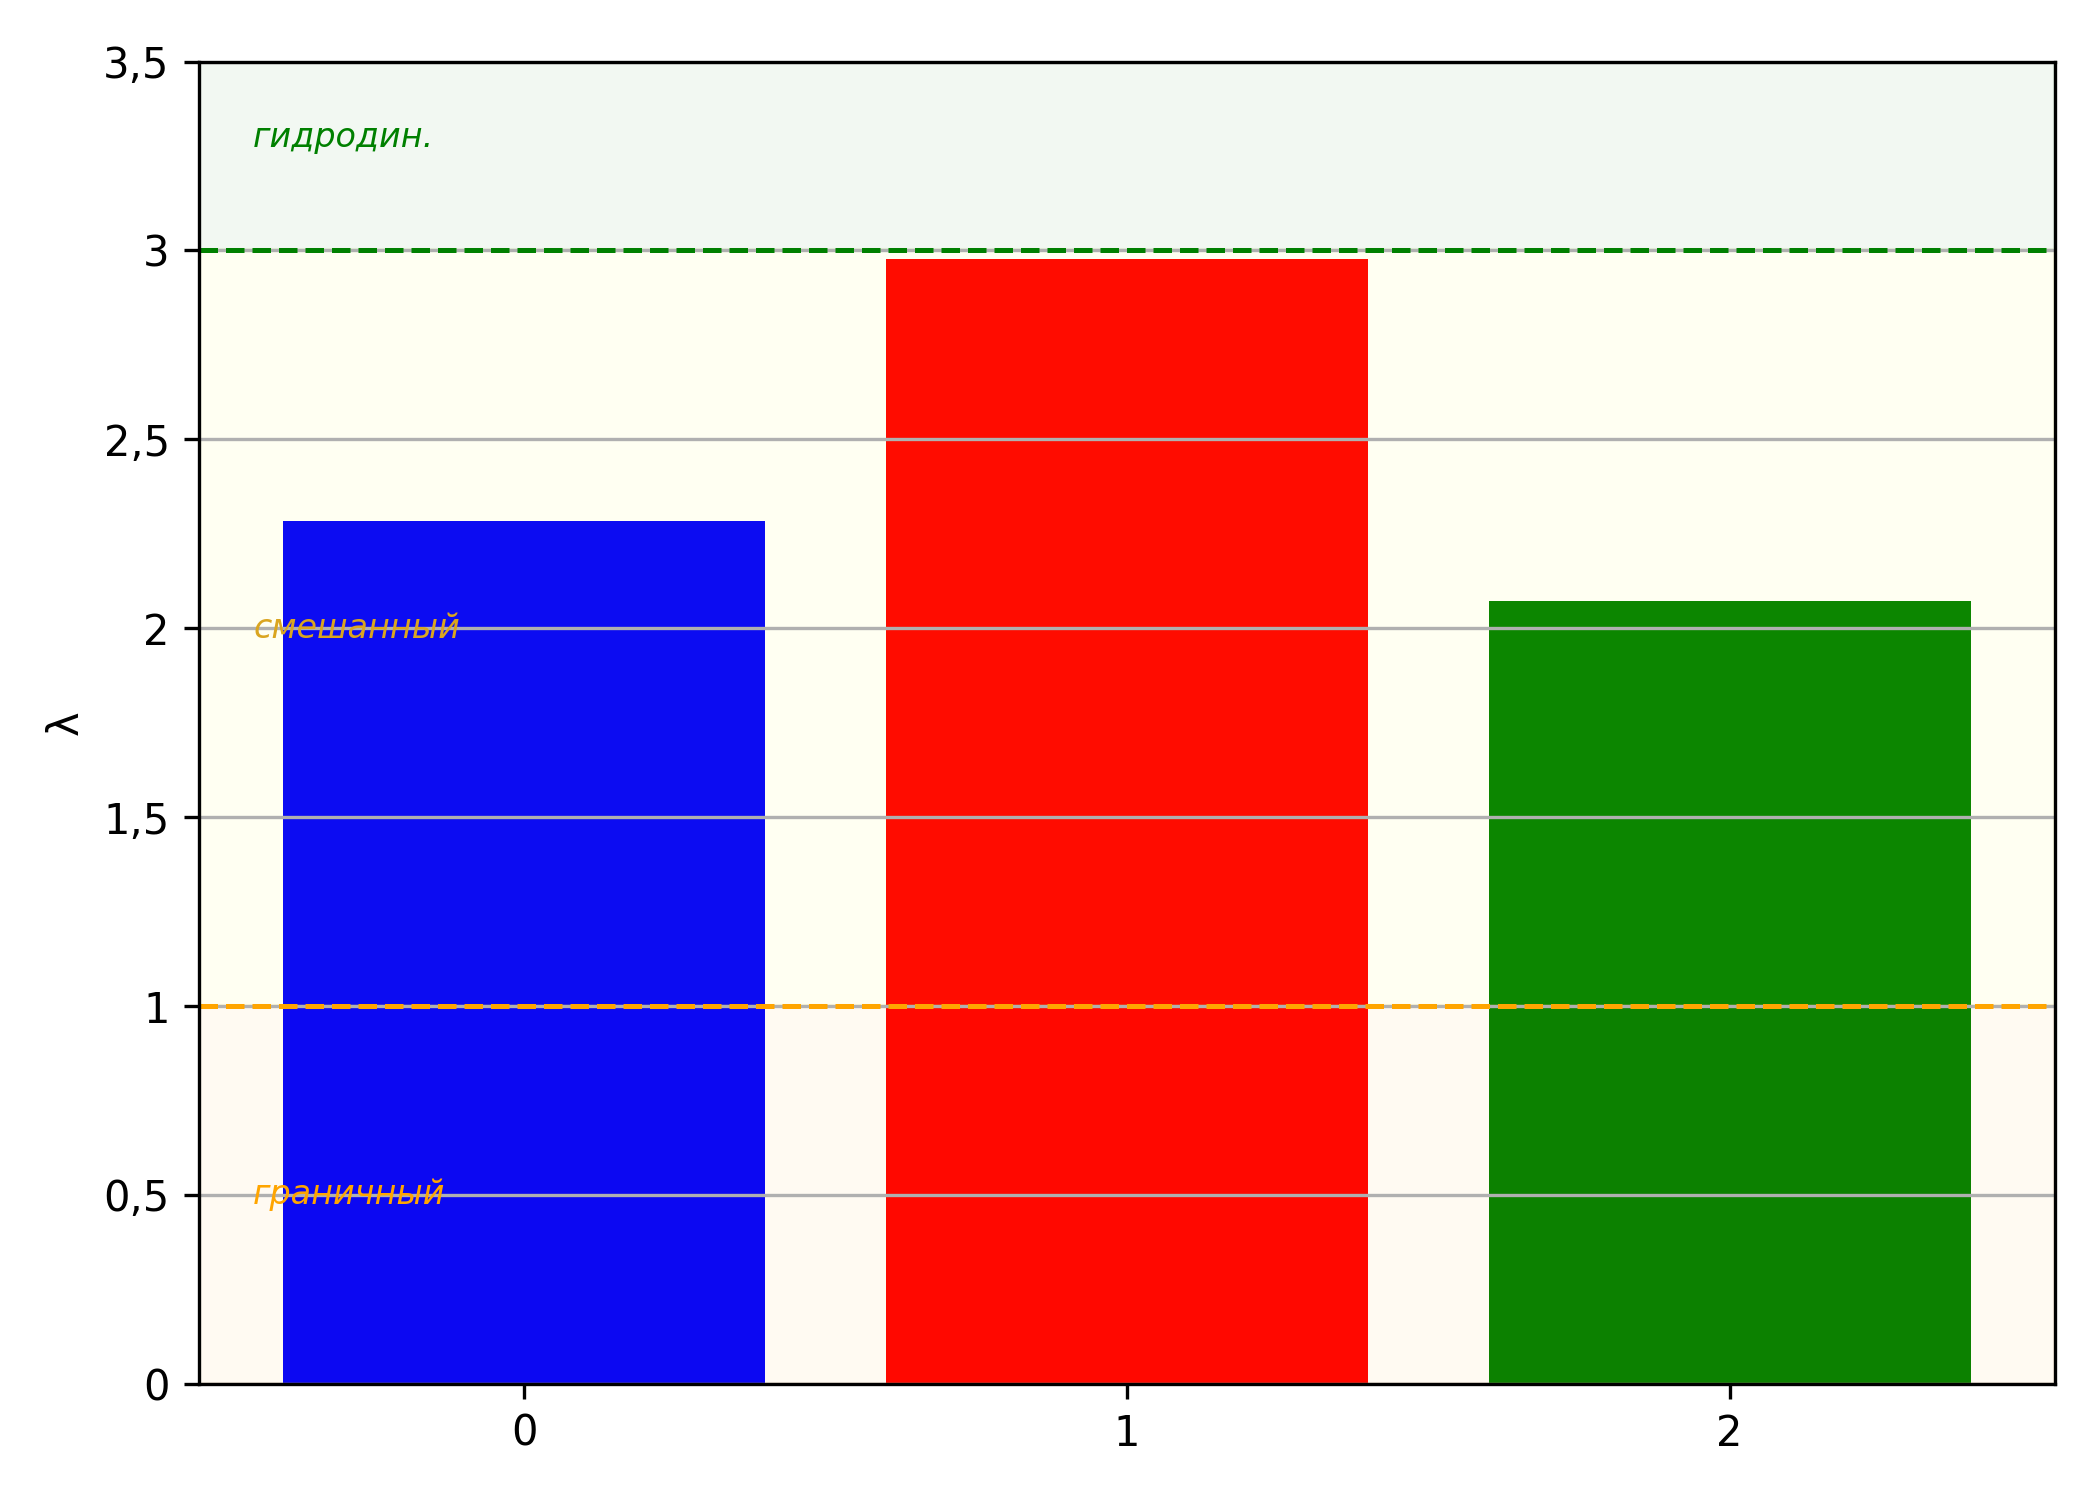
\includegraphics[width=\textwidth,height=0.9\textheight,keepaspectratio]{figures/ch06/fig_6_3.png}
\caption{Параметр плёнки $\lambda$ в рабочей точке ($F_{\mathrm{ext}} = 6\,000$~Н)
  для конфигураций T1, T2, T3. Пунктирные линии~-- границы режимов смазки:
  $\lambda = 1$ и $\lambda = 3$.}
\label{fig:bit_lambda_comparison}
\end{figure}

\FloatBarrier


\textit{Зависимости характеристик от нагрузки.}
Для оценки поведения подшипника при различных условиях нагружения
выполнен параметрический расчёт при~$F_{\mathrm{ext}}$ от
${\sim}\,2100$ до ${\sim}\,6800$~Н. Диапазон ограничен
грузоподъёмностью конфигураций при $\varepsilon = 0{,}97$.

С ростом нагрузки эксцентриситет монотонно возрастает
(рисунок~\ref{fig:bit_sweep_B_epsilon}). При одинаковой
нагрузке конфигурация~T2 имеет наименьший эксцентриситет,
T3~-- наибольший. Конфигурация~T3 достигает расчётного предела
при $F \approx 6200$~Н и теряет рабочую точку раньше, чем T1 и~T2.

\begin{figure}[!ht]
\centering
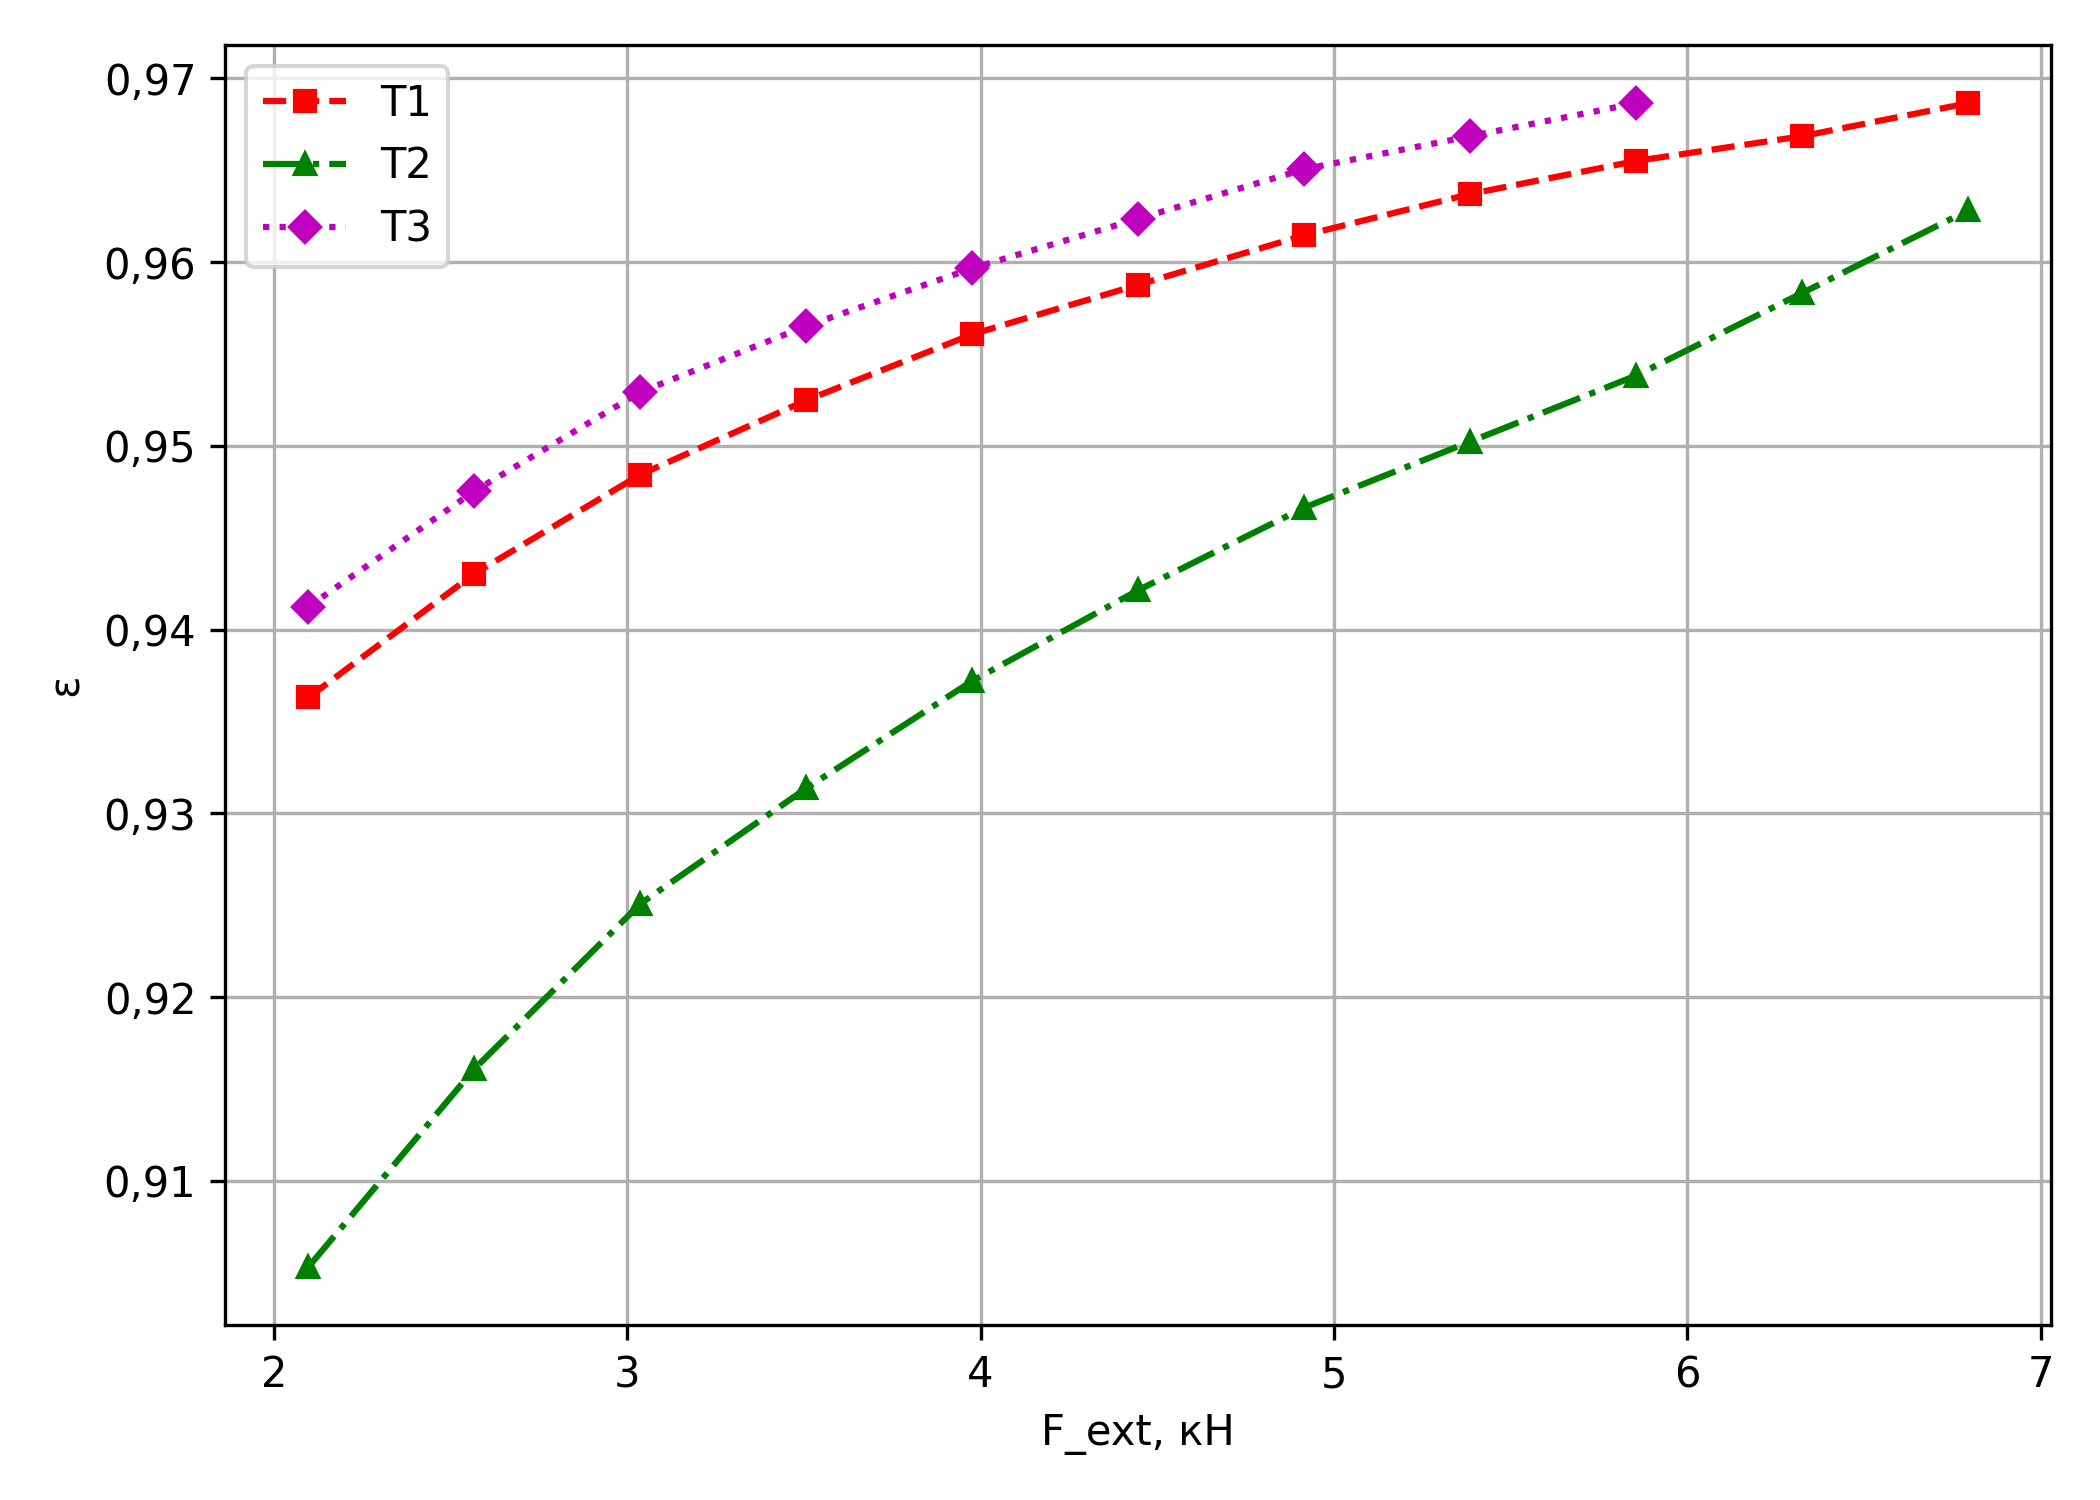
\includegraphics[width=\textwidth,height=0.9\textheight,keepaspectratio]{figures/ch06/fig_6_4.png}
\caption{Зависимость эксцентриситета $\varepsilon$ от нагрузки $F_{\mathrm{ext}}$
  для конфигураций T1, T2, T3 в рабочей зоне текстурированных вариантов.}
\label{fig:bit_sweep_B_epsilon}
\end{figure}

\FloatBarrier

Параметр плёнки~$\lambda$ убывает с ростом нагрузки
(рисунок~\ref{fig:bit_sweep_B_lambda}). При
$F \approx 6\,000$~Н конфигурация~T2 находится вблизи границы
смешанного и гидродинамического режимов ($\lambda \approx 3$);
конфигурации~T1 и~T3 остаются в смешанном режиме ($\lambda < 2{,}5$).

\begin{figure}[!ht]
\centering
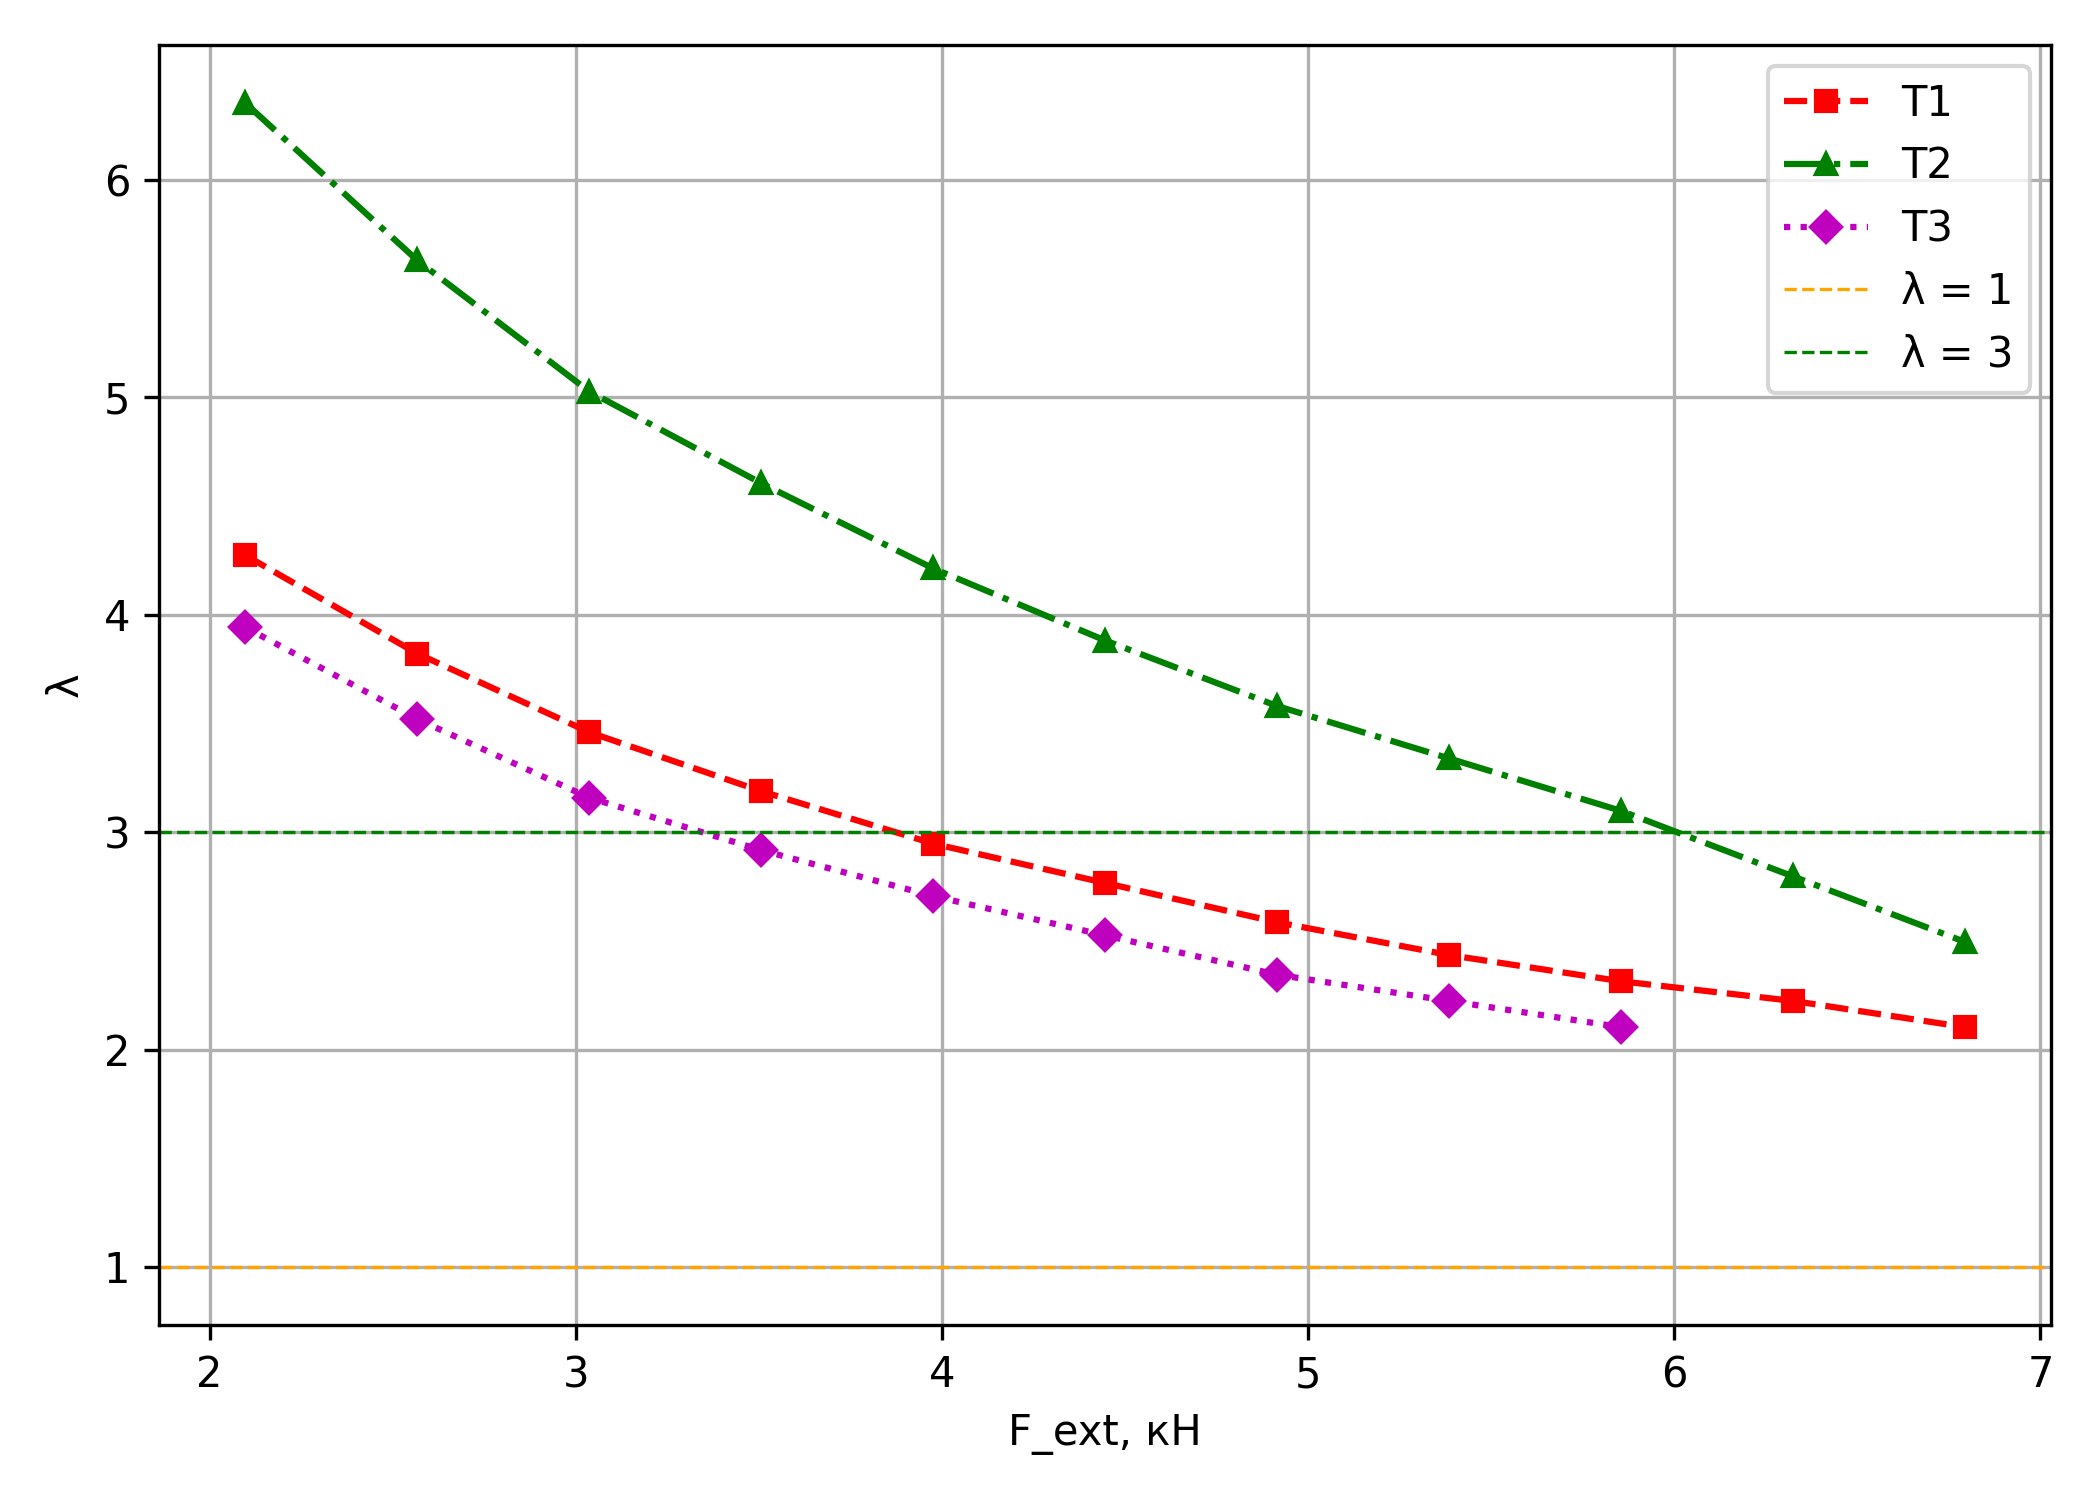
\includegraphics[width=\textwidth,height=0.9\textheight,keepaspectratio]{figures/ch06/fig_6_5.png}
\caption{Зависимость параметра плёнки $\lambda$ от нагрузки $F_{\mathrm{ext}}$.
  Пунктирные линии~-- границы режимов смазки $\lambda = 1$ и $\lambda = 3$.}
\label{fig:bit_sweep_B_lambda}
\end{figure}

\FloatBarrier

Минимальная толщина плёнки~$h_{\min}$ убывает с ростом нагрузки
(рисунок~\ref{fig:bit_sweep_B_hmin}). При $F = 6\,000$~Н:
$h_{\min} = 2{,}66$~мкм (T2), $2{,}04$~мкм (T1), $1{,}85$~мкм (T3),
что сопоставимо с суммарной шероховатостью
$\sigma_{\mathrm{eq}} = 0{,}89$~мкм.

\textit{Коэффициенты улучшения на общей достижимой нагрузке.}
При $F_{\mathrm{ext}} = 6\,000$~Н гладкий подшипник не имеет
рабочей точки, что исключает прямое нормирование характеристик
текстурированных вариантов на значения гладкого при рабочей нагрузке.
Нормированные показатели определяются при общей достижимой нагрузке:

\begin{figure}[!ht]
\centering
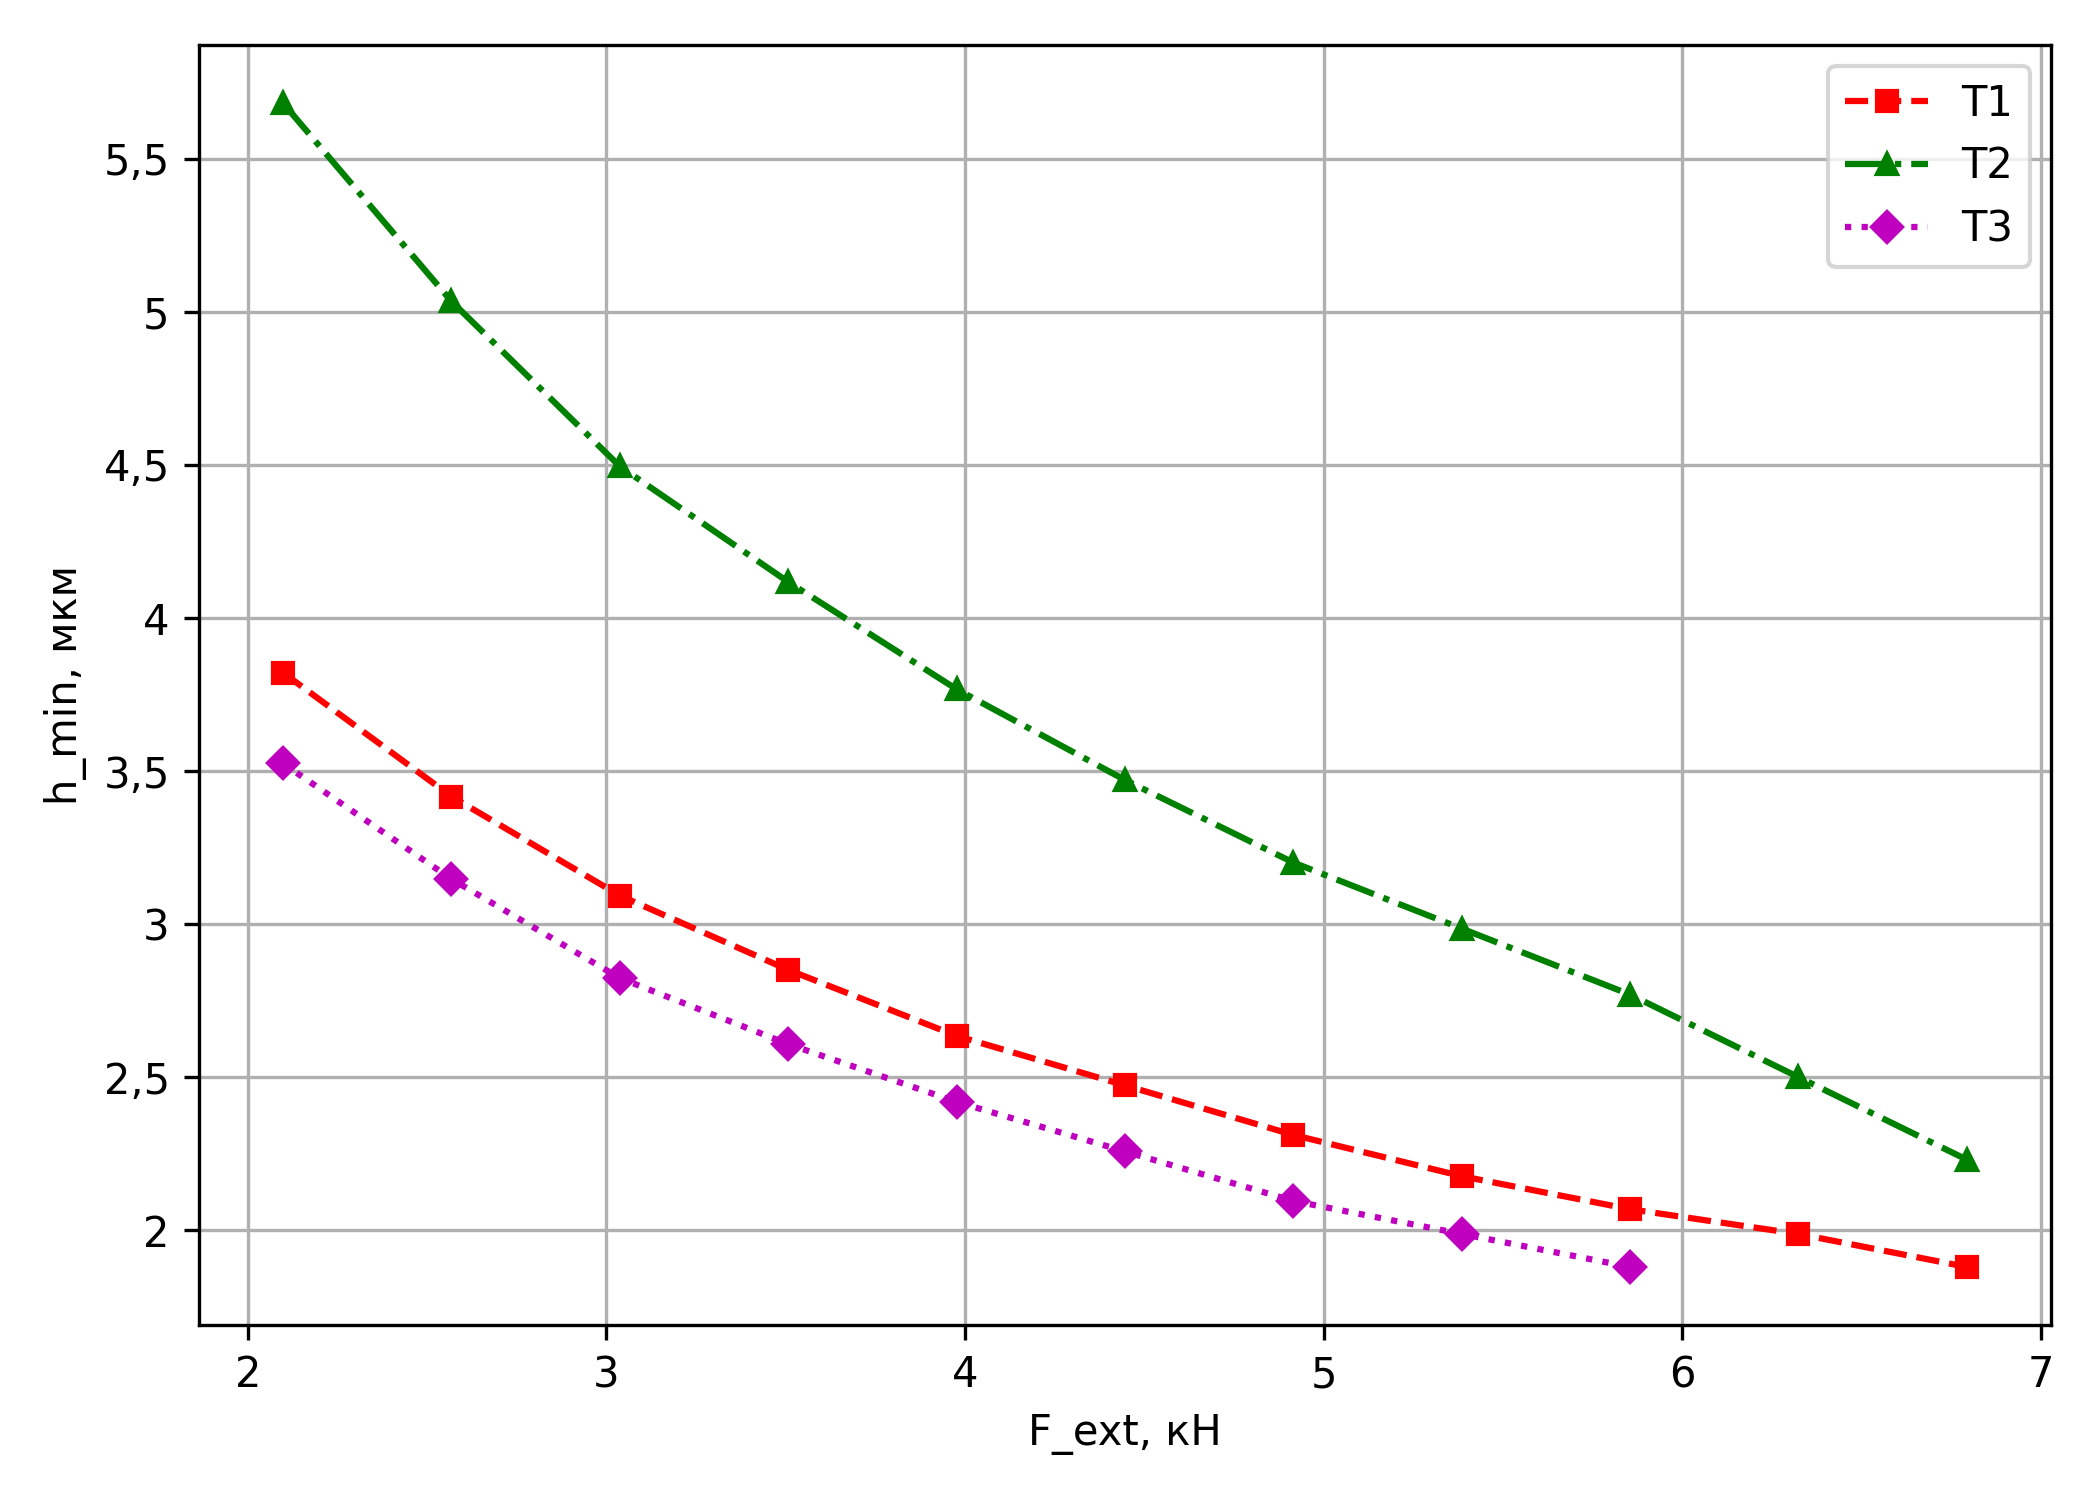
\includegraphics[width=\textwidth,height=0.9\textheight,keepaspectratio]{figures/ch06/fig_6_6.png}
\caption{Зависимость минимальной толщины плёнки $h_{\min}$ от нагрузки
  $F_{\mathrm{ext}}$ для конфигураций T1, T2, T3.}
\label{fig:bit_sweep_B_hmin}
\end{figure}
\begin{equation}
  F_* = 0{,}85 \cdot F_0
    (\varepsilon = 0{,}97) = 1\,621\;\text{Н},
  \label{eq:bit_Fcommon}
\end{equation}
при которой рабочая точка существует у всех вариантов, включая
гладкий.

Нормированные показатели эффективности определяются следующим
образом:
\begin{equation}
\begin{split}
  &G_{h}^{(i)} = \frac{h_{\min}^{(i)}}{h_{\min}^{(0)}},
  \quad
  G_{\lambda}^{(i)} = \frac{\lambda^{(i)}}{\lambda^{(0)}}, \\
  &G_{PV}^{(i)} = \frac{PV^{(0)}}{PV^{(i)}},
  \quad
  G_{w}^{(i)} = \frac{I_w^{(0)}}{I_w^{(i)}}.
\end{split}
  \label{eq:bit_gain_factors}
\end{equation}
где верхний индекс~$(0)$~-- гладкий вариант,
$(i)$~-- текстурированные конфигурации T1, T2, T3.
Значение~$G > 1$ желательно для всех четырёх показателей.

Результаты расчёта нормированных показателей при
$F_* = 1\,621$~Н сведены в
таблицу~\ref{tab:bit_gains}.

\begin{table}[!ht]
\centering
\caption{Нормированные показатели эффективности при
  $F_* = 1\,621$~Н}
\label{tab:bit_gains}
\begin{tabularx}{\textwidth}{|X|c|c|c|c|}
\hline
\multicolumn{1}{|c|}{\textbf{Конфигурация}}
  & $\boldsymbol{G_h}$
  & $\boldsymbol{G_{\lambda}}$
  & $\boldsymbol{G_{PV}}$
  & $\boldsymbol{G_w}$ \\
\hline
T1 & 2{,}119 & 2{,}119 & 1{,}009 & 2{,}137 \\
\hline
T2 & 3{,}147 & 3{,}147 & 1{,}002 & 3{,}153 \\
\hline
T3 & 1{,}964 & 1{,}964 & 0{,}996 & 1{,}956 \\
\hline
\end{tabularx}
\end{table}

\FloatBarrier

Конфигурация~T2 обеспечивает $G_h = 3{,}147$
и $G_{\lambda} = 3{,}147$~-- утроение минимального зазора
и параметра плёнки по сравнению с гладким подшипником.
Показатель~$G_{PV}$ у всех конфигураций близок к единице:
при фиксированной нагрузке номинальное давление~$p_0$
практически не изменяется, и основной эффект текстурирования
реализуется через снижение эксцентриситета и рост зазора,
а не через изменение~$PV$. У конфигурации~T3
$G_{PV} = 0{,}996 < 1$~-- незначительный рост~$PV$, согласующийся
с меньшей несущей способностью этой конфигурации.

Нормированные показатели наглядно сопоставлены на
рисунке~\ref{fig:bit_gains_common}.

\begin{figure}[!ht]
\centering
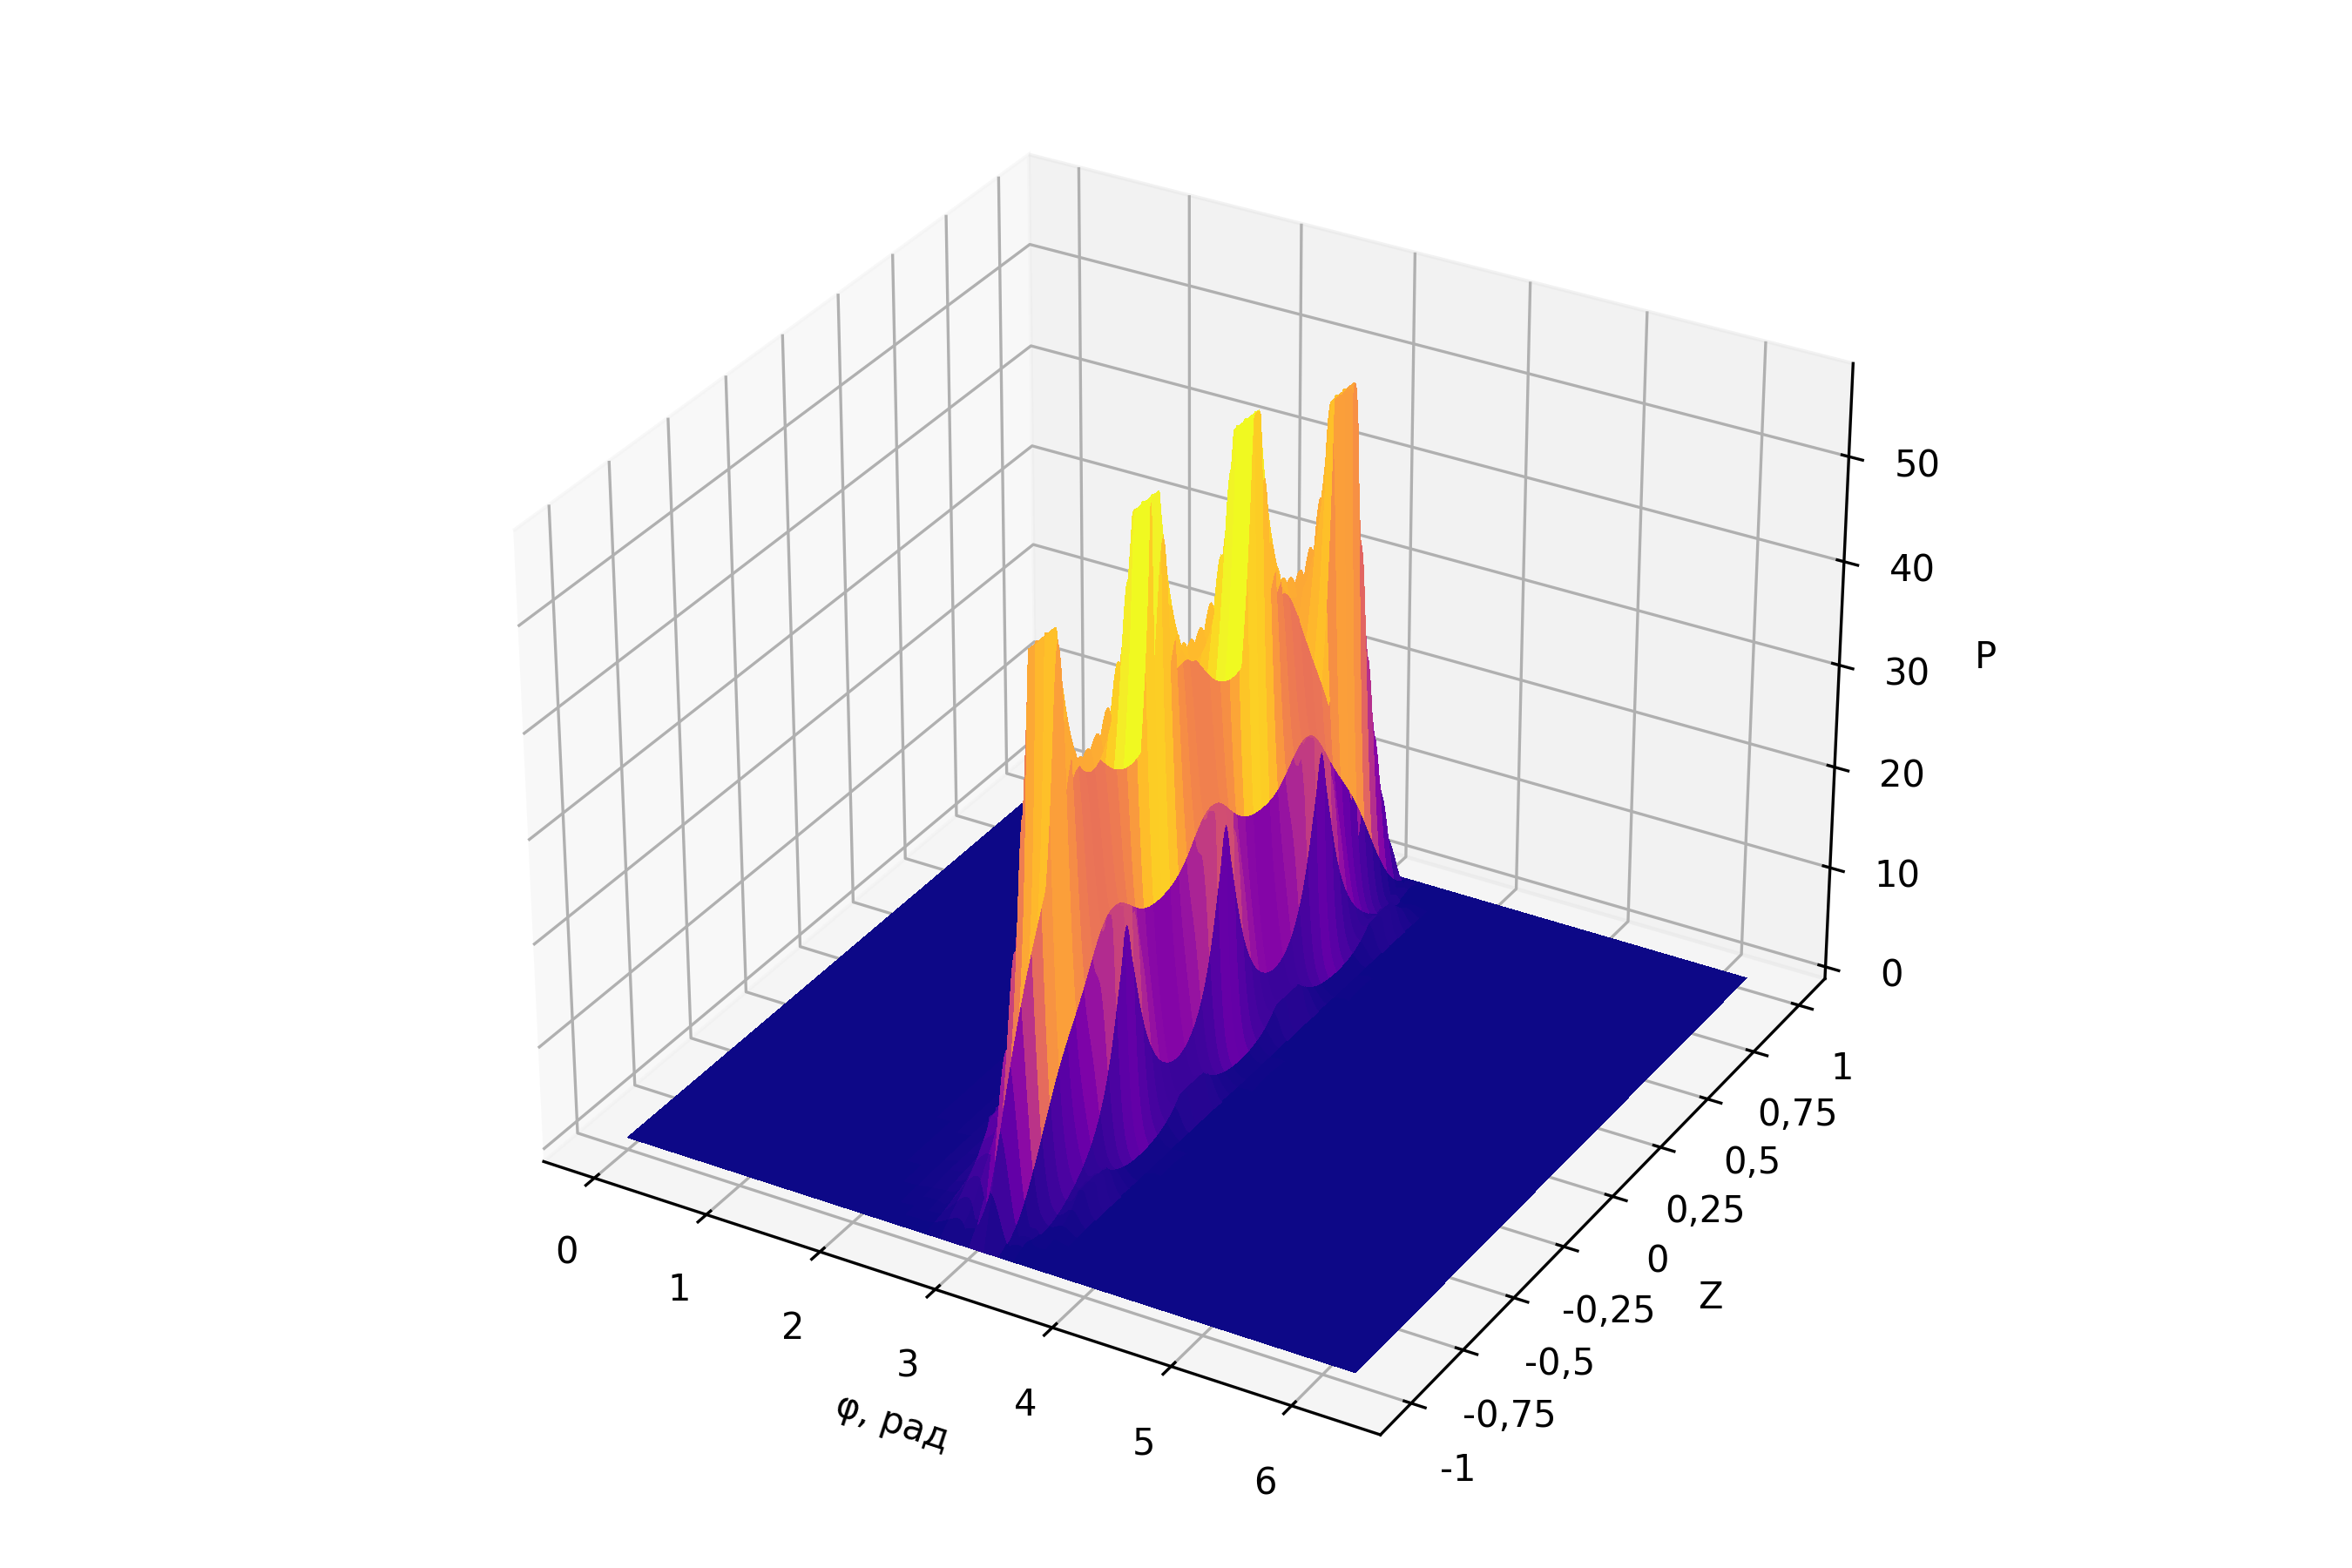
\includegraphics[width=\textwidth,height=0.9\textheight,keepaspectratio]{figures/ch06/fig_6_7.png}
\caption{Нормированные показатели эффективности $G_h$, $G_{\lambda}$,
  $G_{PV}$, $G_w$ для конфигураций T1, T2, T3
  при $F_* = 1\,621$~Н.
  Пунктирная горизонталь $G = 1$~-- уровень гладкого подшипника.}
\label{fig:bit_gains_common}
\end{figure}

\FloatBarrier


\textit{Поле давления лучшей конфигурации.}
Для конфигурации~T2, продемонстрировавшей наилучшие характеристики,
представлено трёхмерное поле безразмерного давления~$P(\theta, Z)$
в рабочей точке ($\varepsilon = 0{,}956$). Зона максимального
давления располагается вблизи $\theta \approx \pi$. Лунки
конфигурации~T2 формируют выраженную <<рябь>> на поверхности
давления, свидетельствующую о локальном перераспределении потоков
в каждом элементе микрорельефа
(рисунок~\ref{fig:bit_P3D_T2}).

\begin{figure}[!ht]
\centering
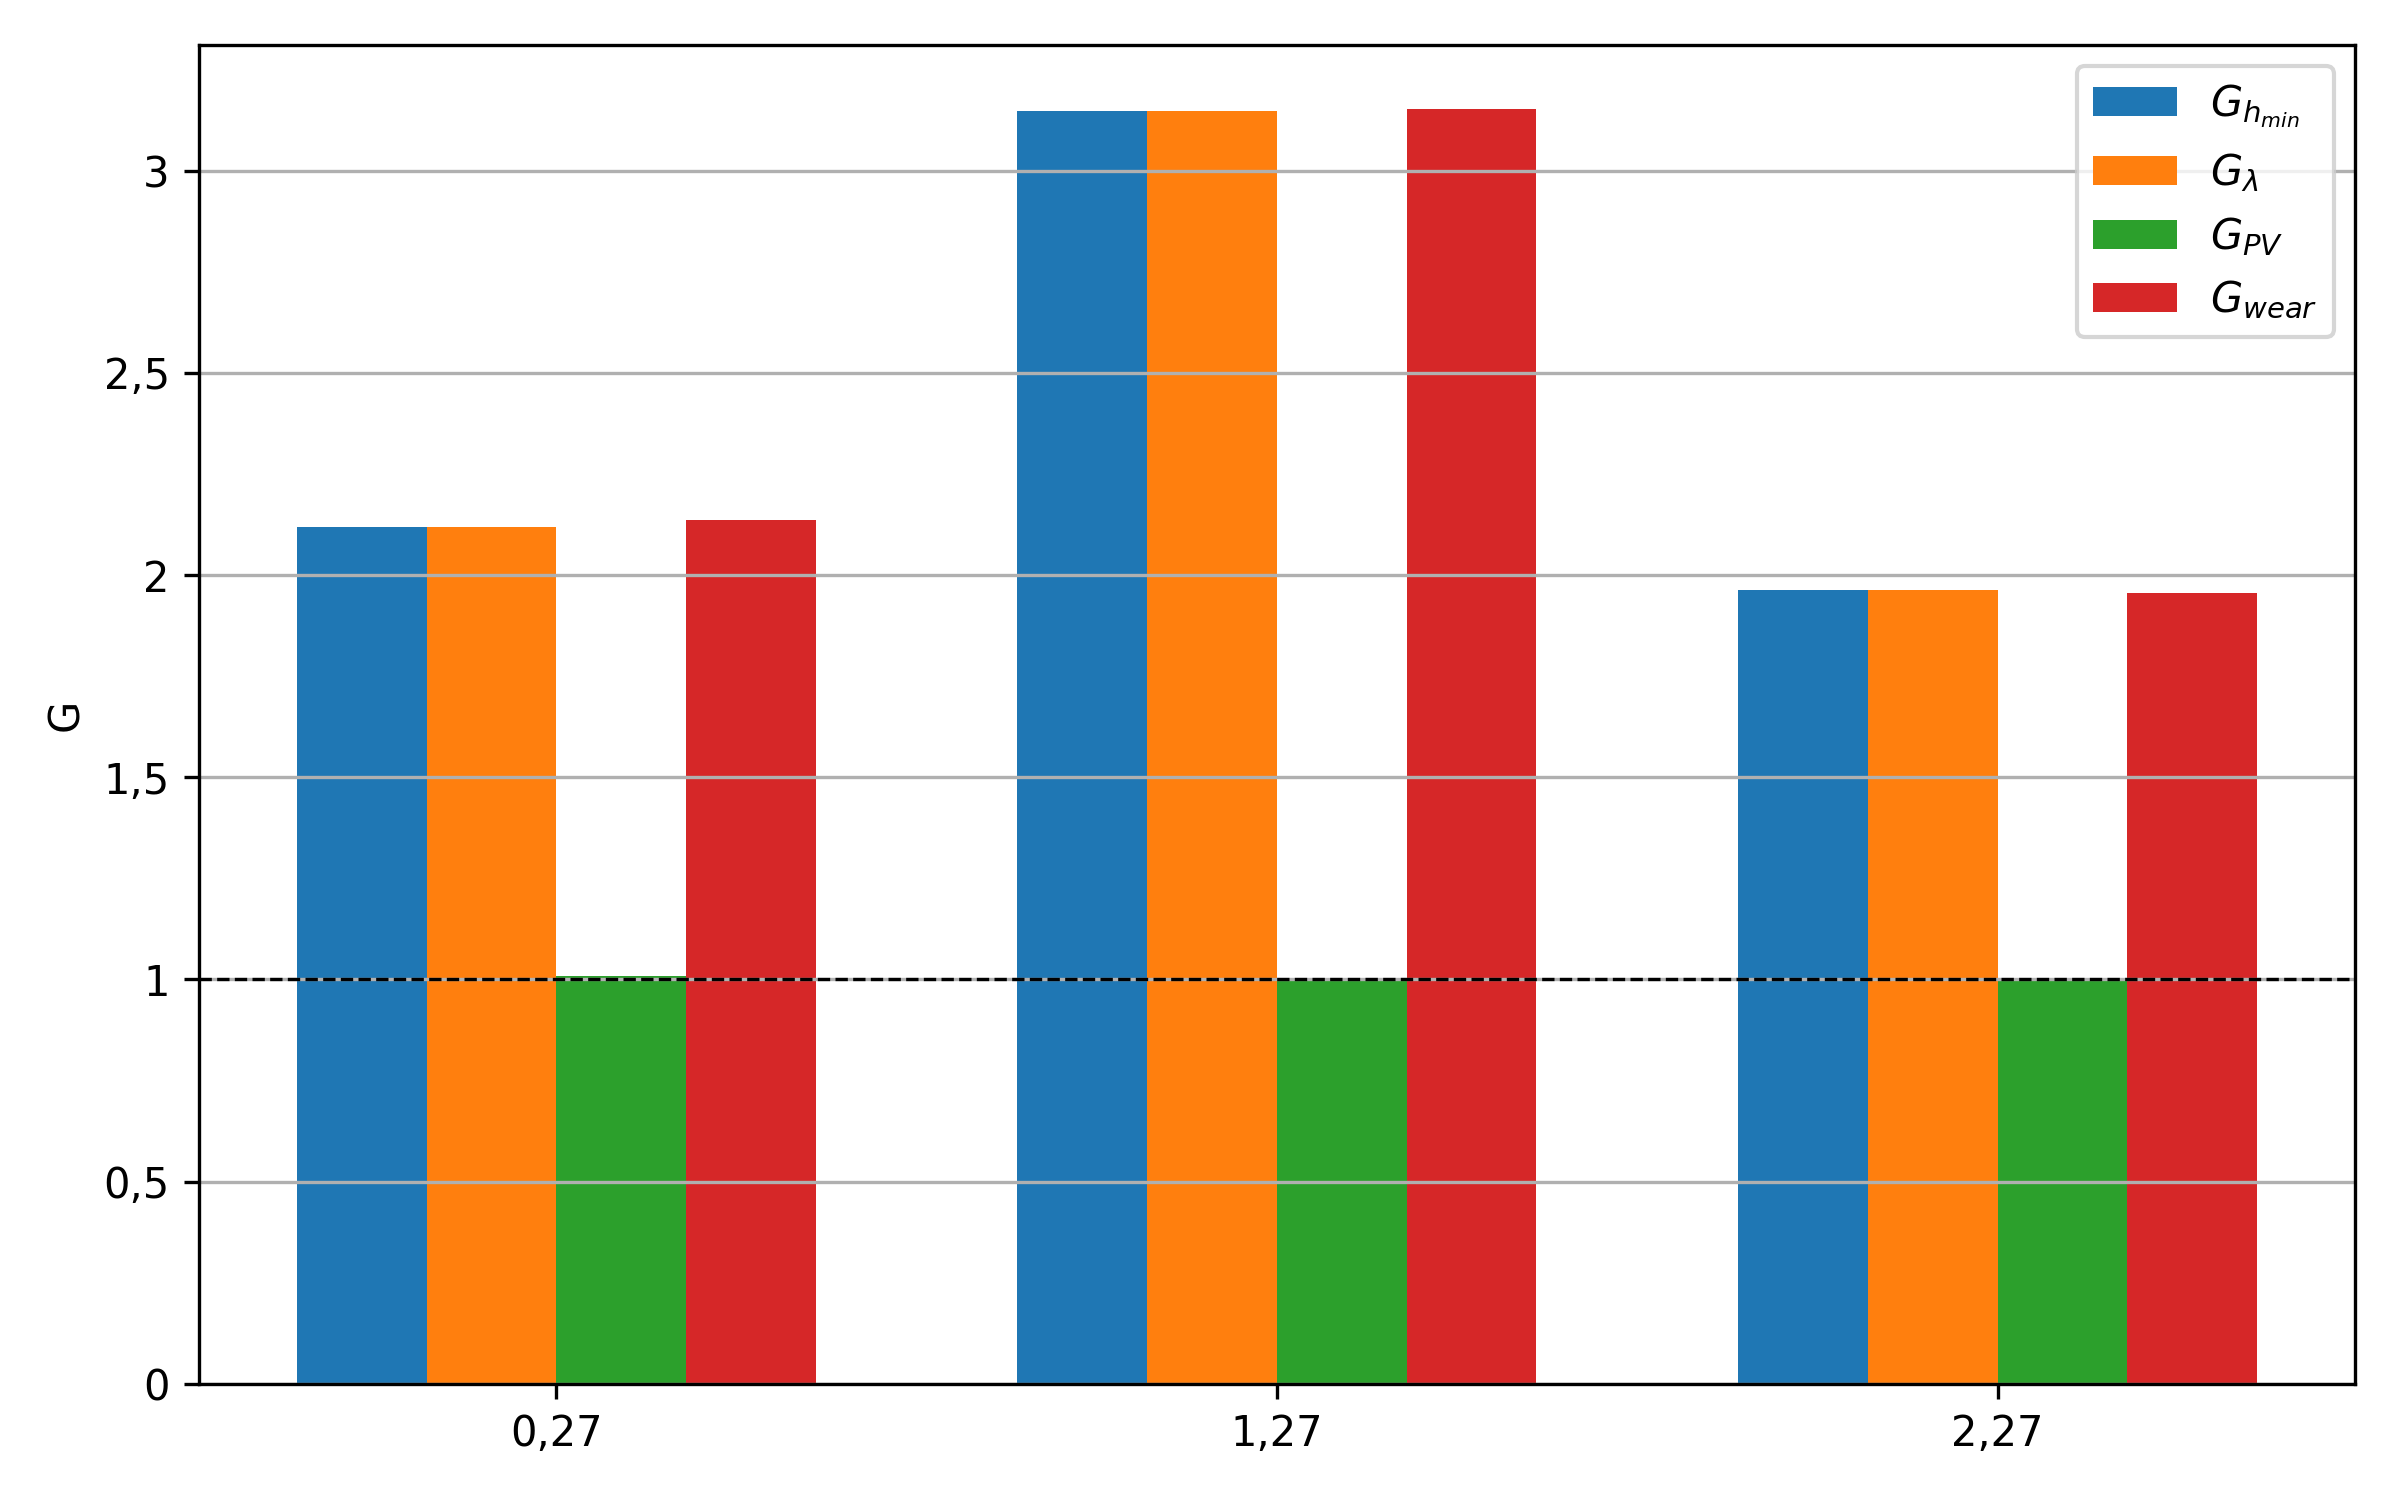
\includegraphics[width=\textwidth,height=0.9\textheight,keepaspectratio]{figures/ch06/fig_6_8.png}
\caption{Поле безразмерного давления $P(\theta, Z)$
  для конфигурации~T2 ($H_p = 0{,}40$, зона $90^{\circ}$--$270^{\circ}$)
  в рабочей точке $\varepsilon = 0{,}956$.}
\label{fig:bit_P3D_T2}
\end{figure}


\FloatBarrier
\section*{Выводы по главе~6}
\phantomsection\addcontentsline{toc}{section}{Выводы по главе~6}

Проведён анализ радиального подшипника скольжения опоры шарошки
трёхшарошечного долота в изотермическом приближении с учётом
кавитации по условию Рейнольдса ($P \geq 0$). Установлено, что
гладкий подшипник при рабочей нагрузке
$F_{\mathrm{ext}} = 6\,000$~Н не имеет равновесной рабочей точки
в чисто гидродинамической постановке:
$F(\varepsilon = 0{,}97) = 1907$~Н.

Текстурирование поверхности цапфы эллипсоидальными лунками
в шахматной раскладке существенно повышает гидродинамическую
несущую способность: $F(\varepsilon = 0{,}97)$ достигает
$7549$~Н (конфигурация~T2), что в~$3{,}96$ раза превышает
значение гладкого варианта. Рабочая точка при
$F_{\mathrm{ext}} = 6\,000$~Н найдена для всех конфигураций
T1--T3.

В рабочих точках все конфигурации функционируют в смешанном режиме
смазки ($\lambda \approx 2{,}1$--$3{,}0$). Конфигурация~T2
($H_p = 0{,}40$, зона $90^{\circ}$--$270^{\circ}$) демонстрирует
наилучшие показатели: $\varepsilon = 0{,}956$,
$h_{\min} = 2{,}66$~мкм, $\lambda = 2{,}98$~-- значение,
наиболее близкое к границе гидродинамического режима.

На общей достижимой нагрузке $F_* = 1\,621$~Н
конфигурация~T2 обеспечивает трёхкратное увеличение минимального
зазора ($G_h = 3{,}15$) и параметра плёнки
($G_{\lambda} = 3{,}15$). Показатели~$G_{PV}$ близки к единице
(фиксированная нагрузка); основной эффект текстурирования
реализуется через рост минимального зазора и улучшение условий
смазки.

Анализ упорного подшипника скольжения с детерминированными
микроструктурами выполнен в главе~7.



\section{Пример анализа упорного подшипника скольжения}

Третий пример демонстрирует расчёт упорного подшипника скольжения с~секторными колодками. В~отличие от~радиальных подшипников, рассмотренных выше, несущая способность упорного подшипника обусловлена клиновым зазором между колодкой и~диском, а~задача формулируется в~цилиндрических координатах. Пример позволяет студенту освоить постановку задачи и~методику расчёта для~принципиально иного типа подшипника.

% =============================================================
% 7 Анализ упорного подшипника скольжения
% =============================================================
\chapter{Анализ рельефного упорного подшипника скольжения}

\section{Объект исследования и исходные данные}

Объектом исследования в настоящей главе является упорный подшипник
скольжения с секторными колодками~\cite{gropper2018,wasilczuk2008}. Неподвижные колодки удерживают
осевую нагрузку вращающегося диска (ротора). Подшипник состоит
из~$N_{\mathrm{pads}} = 6$ одинаковых секторных колодок; расчёт
ведётся для одного сектора с последующим пересчётом интегральных
характеристик на полный подшипник.

В отличие от радиального подшипника (главы~5 и~6), где несущая сила
обусловлена эксцентриситетом цапфы, в упорном подшипнике давление
возникает вследствие клинового зазора между колодкой и диском.
Основным геометрическим параметром является параметр клина
$K = h_{\mathrm{in}} / h_{\mathrm{out}}$, где
$h_{\mathrm{in}}$~-- зазор на входной кромке сектора,
$h_{\mathrm{out}}$~-- зазор на выходной кромке.
Характер уравнения Рейнольдса также отличается: задача формулируется
в цилиндрических координатах $(r, \theta)$, а скорость скольжения
зависит от радиуса: $U(r) = \omega \cdot r$~\cite{brajdic2005,heinrichson2008}.

Основные параметры подшипника сведены в
таблицу~\ref{tab:thrust_params}.

\begin{table}[!ht]
\centering
\caption{Параметры упорного подшипника скольжения}
\label{tab:thrust_params}
\begin{tabularx}{\textwidth}{|X|c|c|c|}
\hline
\multicolumn{1}{|c|}{\textbf{Параметр}} & \textbf{Обозначение} & \textbf{Значение} & \textbf{Единица} \\
\hline
Внутренний радиус          & $R_{\mathrm{in}}$   & 30{,}0  & мм \\
\hline
Наружный радиус            & $R_{\mathrm{out}}$  & 60{,}0  & мм \\
\hline
Число колодок              & $N_{\mathrm{pads}}$ & 6       & -- \\
\hline
Угол сектора               & $\beta = 2\pi/N$    & 60{,}0  & $^{\circ}$ \\
\hline
Минимальный зазор          & $h_{\mathrm{out}}$  & 50      & мкм \\
\hline
Номинальный параметр клина & $K_{\mathrm{nom}}$  & 2{,}0   & -- \\
\hline
Динамическая вязкость      & $\mu$               & 0{,}020 & Па$\cdot$с \\
\hline
Частота вращения           & $n$                 & 3000    & об/мин \\
\hline
Угловая скорость           & $\omega$            & 314{,}2 & рад/с \\
\hline
\end{tabularx}
\end{table}

\FloatBarrier

Схема сектора упорного подшипника представлена на
рисунке~\ref{fig:thrust_scheme}.

\begin{figure}[!ht]
\centering
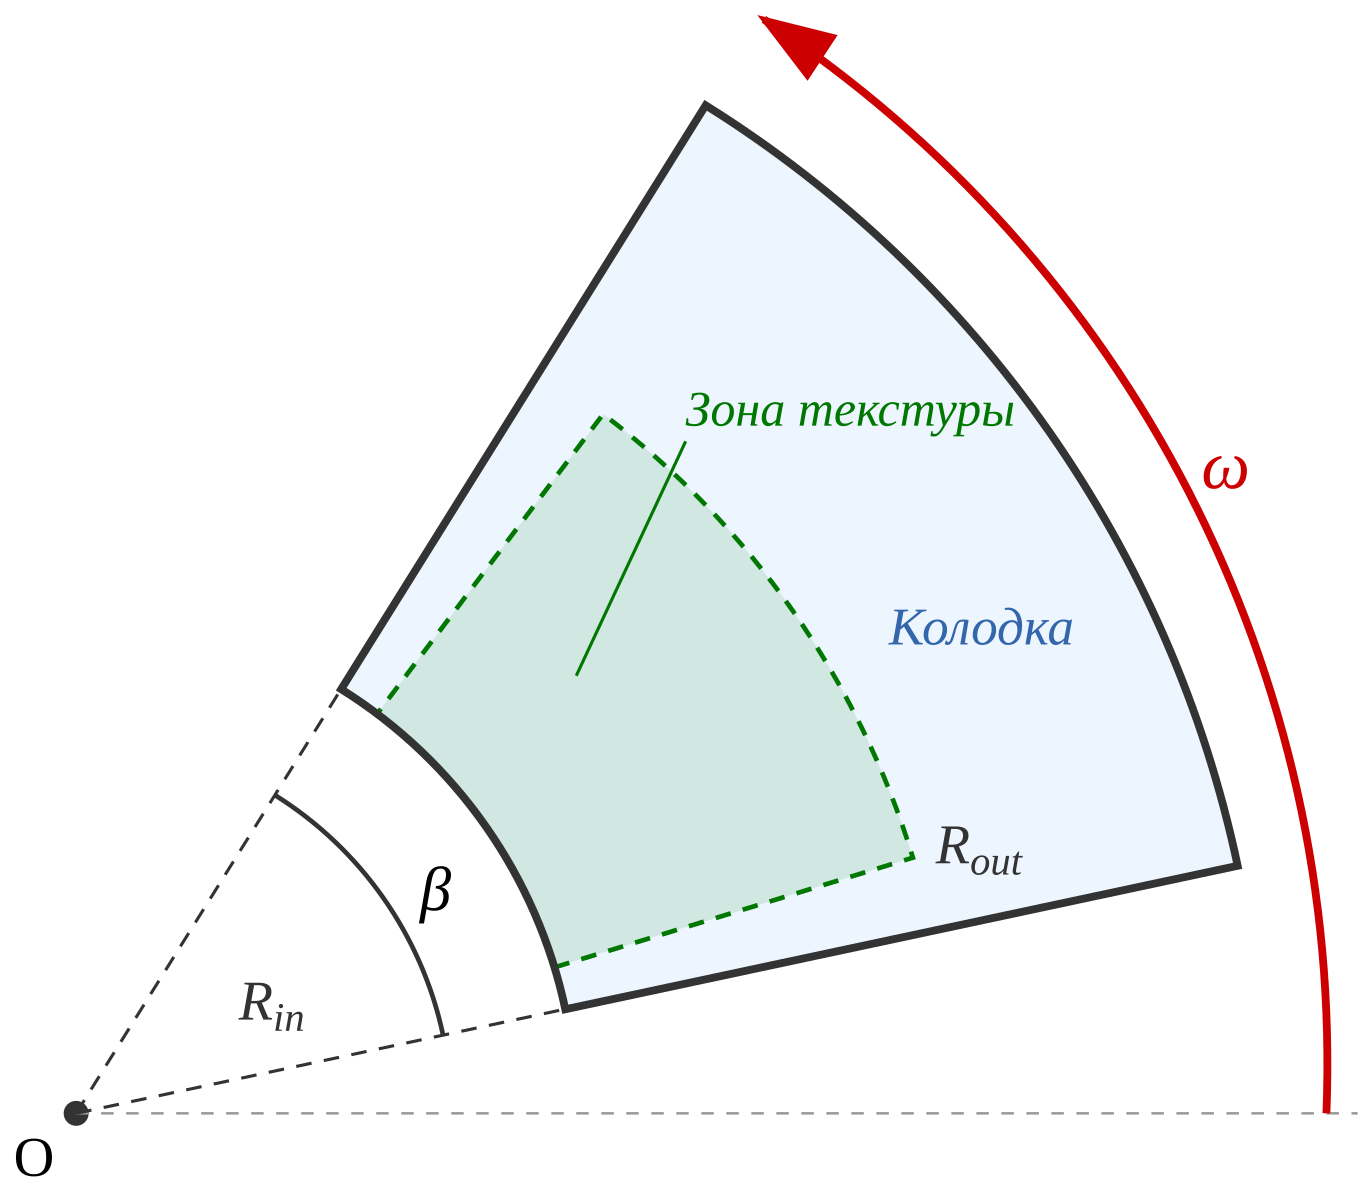
\includegraphics[width=\textwidth,height=0.9\textheight,keepaspectratio]{figures/ch07/fig_7_1.png}
\caption{Расчётная схема сектора упорного подшипника скольжения}
\label{fig:thrust_scheme}
\end{figure}

\FloatBarrier


\section{Расчётная схема и математическая модель}

Расчётная область представляет собой развёртку поверхности одного
сектора: $r \in [R_{\mathrm{in}},\, R_{\mathrm{out}}]$,
$\theta \in [0,\, \beta]$.

Угловая скорость вращения диска определяется частотой вращения:
\begin{equation}
  \omega = \frac{2\pi n}{60}.
  \label{eq:thrust_omega}
\end{equation}
Скорость скольжения на радиусе~$r$:
\begin{equation}
  U(r) = \omega \cdot r.
  \label{eq:thrust_U}
\end{equation}

Толщина смазочного зазора между колодкой и диском определяется
линейным законом клина:
\begin{equation}
  h(r, \theta) = h_{\mathrm{out}}
    + (h_{\mathrm{in}} - h_{\mathrm{out}})
    \left(1 - \frac{\theta}{\beta}\right)
  = h_{\mathrm{out}}
    \left[1 + (K - 1)\left(1 - \frac{\theta}{\beta}\right)\right],
  \label{eq:thrust_h}
\end{equation}
где $K = h_{\mathrm{in}} / h_{\mathrm{out}}$~-- параметр клина
($K > 1$). При $\theta = 0$ (входная кромка) зазор максимален
$h = h_{\mathrm{in}} = K \cdot h_{\mathrm{out}}$; при
$\theta = \beta$ (выходная кромка) зазор минимален
$h = h_{\mathrm{out}}$.

Распределение давления в смазочном слое описывается уравнением
Рейнольдса в цилиндрических координатах:
\begin{equation}
  \frac{\partial}{\partial r}
    \left[r\, h^3\, \frac{\partial p}{\partial r}\right]
  + \frac{\partial}{\partial \theta}
    \left[\frac{h^3}{r}\, \frac{\partial p}{\partial \theta}\right]
  = 6\mu\omega\, r\, \frac{\partial h}{\partial \theta}.
  \label{eq:thrust_reynolds}
\end{equation}

Граничные условия:
\begin{equation}
\left\{\;
\begin{aligned}
  p &= 0 \quad \text{при } \theta = 0
    \quad \text{(входная кромка)}, \\
  p &= 0 \quad \text{при } \theta = \beta
    \quad \text{(выходная кромка)}, \\
  p &= 0 \quad \text{при } r = R_{\mathrm{in}},\;
    r = R_{\mathrm{out}}.
\end{aligned}
\right.
  \label{eq:thrust_bc}
\end{equation}
Условие кавитации: $p \geq 0$.

Условия $p = 0$ на радиальных кромках представляют собой упрощение
модели, принятое для сравнительного анализа гладкого
и текстурированного вариантов на одной и той же расчётной области.

Интегральные характеристики подшипника вычисляются следующим
образом. Несущая сила:
\begin{equation}
  W = N_{\mathrm{pads}} \iint p\, r\, \mathrm{d}r\, \mathrm{d}\theta.
  \label{eq:thrust_W}
\end{equation}
Момент трения (упрощённая оценка; напорная составляющая
не учитывается):
\begin{equation}
  M_f = N_{\mathrm{pads}} \iint
    \frac{\mu\, \omega\, r}{h}\, r^2\,
    \mathrm{d}r\, \mathrm{d}\theta.
  \label{eq:thrust_Mf}
\end{equation}
Средний радиус:
\begin{equation}
  R_m = \frac{2}{3}\,
    \frac{R_{\mathrm{out}}^3 - R_{\mathrm{in}}^3}
         {R_{\mathrm{out}}^2 - R_{\mathrm{in}}^2}.
  \label{eq:thrust_Rm}
\end{equation}
Коэффициент трения:
\begin{equation}
  f_T = \frac{M_f}{W \cdot R_m}.
  \label{eq:thrust_fT}
\end{equation}
Расход смазочного материала:
\begin{equation}
  Q = N_{\mathrm{pads}} \int
    \left(-\frac{h^3}{12\mu}\,
    \frac{\partial p}{\partial r}\right)
    r\, \mathrm{d}\theta
    \bigg|_{r = R_{\mathrm{out}}}.
  \label{eq:thrust_Q}
\end{equation}
Максимальное давление в секторе:
$p_{\max} = \max\limits_{r,\theta} p(r, \theta)$.


\section{Конфигурации детерминированных микроструктур}

Аналогично главам~5 и~6, в качестве элементов рельефа используются
эллипсоидальные лунки~\eqref{eq:profile_ellipsoidal}
с шахматной раскладкой~\eqref{eq:layout_staggered}.
В координатах $(r, \theta)$ добавка от лунки записывается
в виде:
\begin{equation}
  \Delta h = H_p \cdot h_{\mathrm{out}}
    \left(1 - \frac{\Delta r^2}{a_r^2}
    - \frac{\Delta\theta^2}{a_\theta^2}\right)
  \quad \text{при}\quad
    \frac{\Delta r^2}{a_r^2}
    + \frac{\Delta\theta^2}{a_\theta^2} \leq 1,
  \label{eq:thrust_dimple}
\end{equation}
где $a_r$, $a_\theta$~-- полуоси эллипса в направлениях~$r$
и~$\theta$, $H_p$~-- безразмерная глубина лунки, нормированная
на~$h_{\mathrm{out}}$.

Конфигурации T1 и~T2 нанесены в зоне
$\theta \in [0{,}1\beta;\; 0{,}7\beta]$~-- входная и средняя
часть клина, где давление нарастает. Конфигурация~T3 нанесена
в зоне $\theta \in [0{,}3\beta;\; 0{,}9\beta]$~-- средняя
и выходная часть клина.

Ожидается, что текстурирование в зоне нарастания давления (T1,~T2)
эффективнее, чем в зоне спада (T3), поскольку лунки создают
дополнительные гидродинамические клинья именно там, где формируется
основная несущая способность.

Параметры рассматриваемых конфигураций приведены в
таблице~\ref{tab:thrust_texture}.

\begin{table}[!ht]
\centering
\caption{Параметры конфигураций текстуры упорного подшипника}
\label{tab:thrust_texture}
\begin{tabularx}{\textwidth}{|X|c|c|c|c|c|}
\hline
\multicolumn{1}{|c|}{\textbf{Конфигурация}}
  & $\boldsymbol{H_p}$
  & $\boldsymbol{A^*}$
  & $\boldsymbol{B^*}$
  & \textbf{Зона нанесения}
  & \textbf{Число лунок} \\
\hline
T1 & 0{,}20 & 0{,}060 & 0{,}025 & $0{,}1\beta$--$0{,}7\beta$ & $5 \times 8$ \\
\hline
T2 & 0{,}40 & 0{,}060 & 0{,}025 & $0{,}1\beta$--$0{,}7\beta$ & $5 \times 8$ \\
\hline
T3 & 0{,}20 & 0{,}060 & 0{,}025 & $0{,}3\beta$--$0{,}9\beta$ & $5 \times 8$ \\
\hline
\end{tabularx}
\end{table}

\FloatBarrier

Безразмерные полуоси определяются как
$A^* = a_r / (R_{\mathrm{out}} - R_{\mathrm{in}})$,
$B^* = a_\theta / \beta$.

Карта распределения зазора для конфигурации~T2 представлена
на рисунке~\ref{fig:thrust_texture_map}.

\begin{figure}[!ht]
\centering
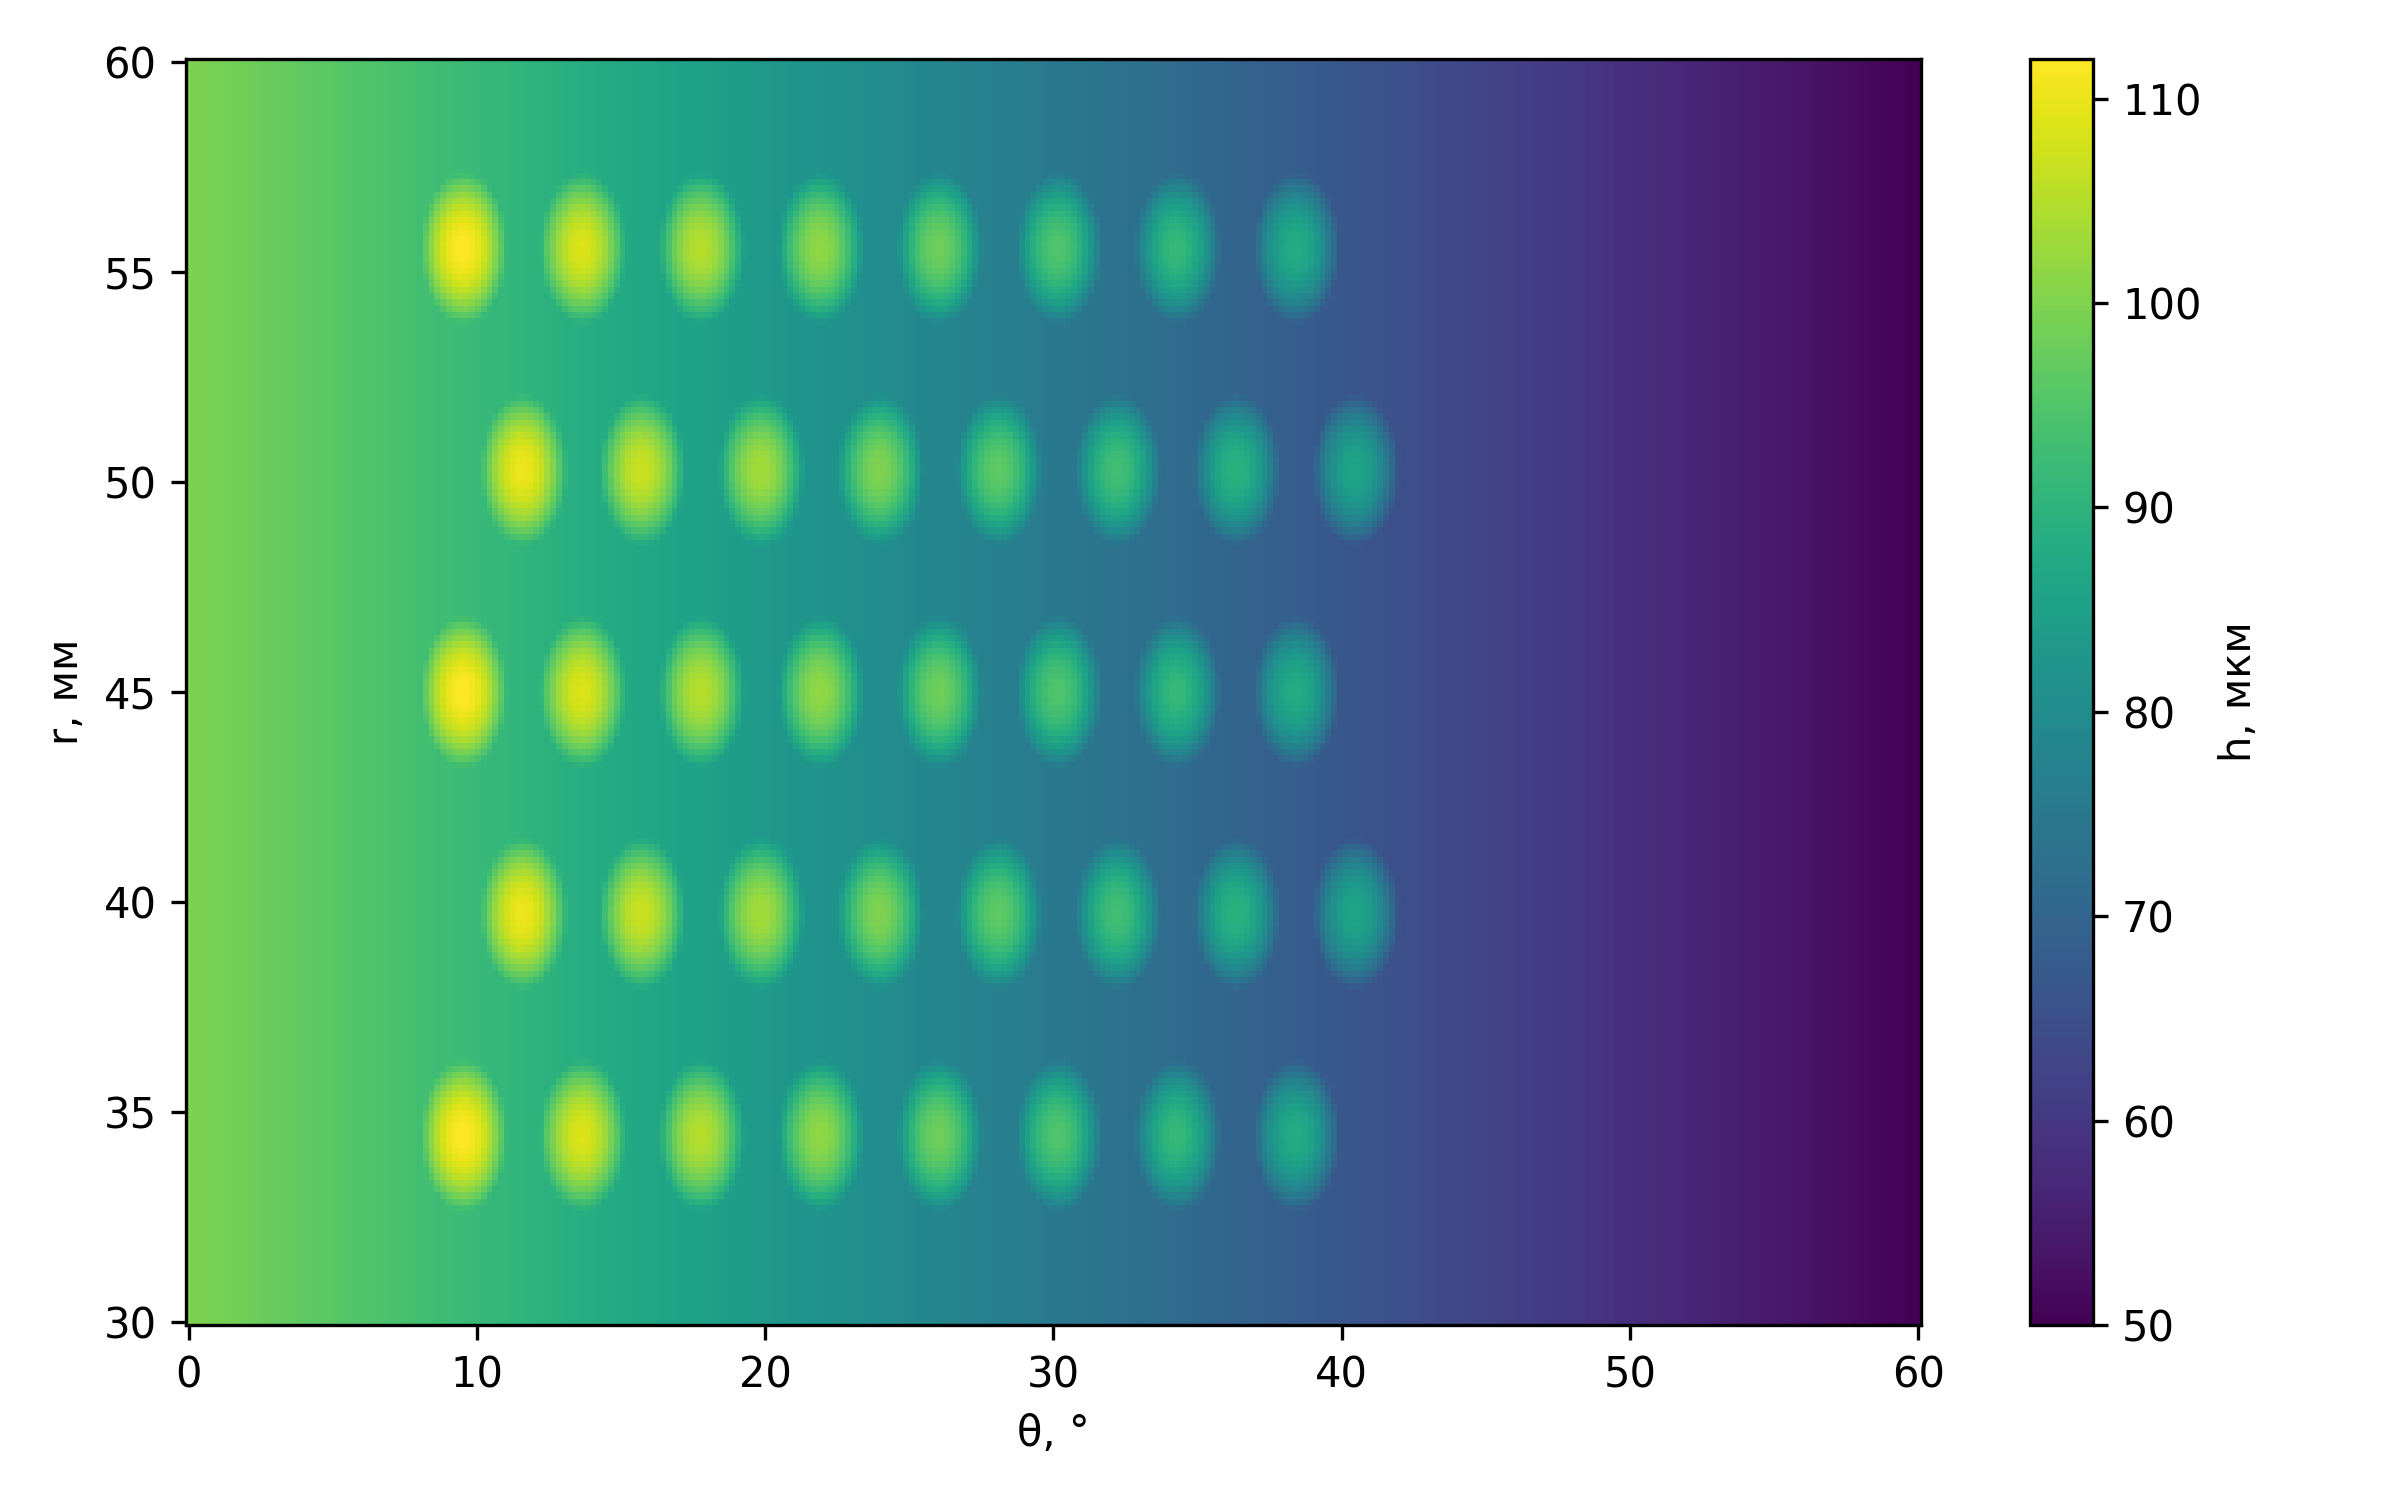
\includegraphics[width=\textwidth,height=0.9\textheight,keepaspectratio]{figures/ch07/fig_7_2.png}
\caption{Карта распределения зазора $h(r, \theta)$ в мкм
  для конфигурации~T2
  ($H_p = 0{,}40$, зона $0{,}1\beta$--$0{,}7\beta$) при $K = 2{,}0$.
  Светлые пятна~-- эллипсоидальные лунки.}
\label{fig:thrust_texture_map}
\end{figure}

\FloatBarrier


\section{Численная реализация расчёта}

Расчётная область дискретизируется равномерной сеткой
$200 \times 300$ узлов по~$r$ и~$\theta$. Уравнение
Рейнольдса~\eqref{eq:thrust_reynolds} аппроксимируется
центральными конечными разностями второго порядка точности.
Коэффициенты дивергентной формы вычисляются на полуузлах
$(i \pm 1/2,\; j \pm 1/2)$ с интерполяцией значений~$h$.

Полученная дискретная система решается итерационным
методом SOR (метод последовательной сверхрелаксации) с параметром
релаксации $\omega_{\mathrm{SOR}} = 1{,}5$. Критерий сходимости:
\begin{equation}
  \frac{\max |P_{\mathrm{new}} - P_{\mathrm{old}}|}
       {\max |P| + 10^{-10}} < 10^{-5}.
  \label{eq:thrust_convergence}
\end{equation}
Кавитация учитывается обнулением отрицательных давлений
на каждой итерации. Сходимость достигается за 2500--8000 итераций
в зависимости от~$K$ и конфигурации текстуры.


\section{Результаты при номинальном параметре клина}

При $K_{\mathrm{nom}} = 2{,}0$ проведён расчёт гладкого
подшипника и конфигураций T1, T2, T3. Результаты приведены
в таблице~\ref{tab:thrust_results}.

\begin{table}[!ht]
\centering
\caption{Характеристики упорного подшипника при $K_{\mathrm{nom}} = 2{,}0$}
\label{tab:thrust_results}
\begin{tabularx}{\textwidth}{|X|c|c|c|c|c|}
\hline
\multicolumn{1}{|c|}{\textbf{Вариант}}
  & $\boldsymbol{W}$, \textbf{кН}
  & $\boldsymbol{M_f}$, \textbf{Н$\cdot$м}
  & $\boldsymbol{f_T}$
  & $\boldsymbol{Q}$, \textbf{мл/с}
  & $\boldsymbol{p_{\max}}$, \textbf{МПа} \\
\hline
Гладкий & 1{,}82 & 1{,}6624 & 0{,}01953 & 26{,}595 & 0{,}510 \\
\hline
T1      & 1{,}84 & 1{,}6458 & 0{,}01912 & 27{,}007 & 0{,}536 \\
\hline
T2      & 1{,}85 & 1{,}6315 & 0{,}01889 & 27{,}324 & 0{,}552 \\
\hline
T3      & 1{,}79 & 1{,}6407 & 0{,}01963 & 26{,}406 & 0{,}523 \\
\hline
\end{tabularx}
\end{table}

\FloatBarrier

В рассматриваемой постановке минимальный зазор определяется
выходной кромкой колодки:
$h_{\min} = h_{\mathrm{out}} = 50$~мкм для всех вариантов
при фиксированной геометрии колодки, поэтому показатель
$G_{h_{\min}} = 1$ для всех конфигураций.

Нормированные показатели эффективности вычисляются аналогично
главам~5 и~6:
\begin{equation}
\begin{split}
  &G_W = \frac{W_{\mathrm{tex}}}{W_{\mathrm{smooth}}}, \quad
  G_{M_f} = \frac{M_{f,\mathrm{smooth}}}{M_{f,\mathrm{tex}}}, \\
  &G_{f_T} = \frac{f_{T,\mathrm{smooth}}}{f_{T,\mathrm{tex}}}, \quad
  G_Q = \frac{Q_{\mathrm{smooth}}}{Q_{\mathrm{tex}}}, \quad
  G_{p_{\max}} = \frac{p_{\max,\mathrm{smooth}}}{p_{\max,\mathrm{tex}}}.
\end{split}
  \label{eq:thrust_gains}
\end{equation}
Значение~$G > 1$ желательно для~$G_W$, $G_{M_f}$, $G_{f_T}$
(рост несущей способности, снижение момента трения и коэффициента
трения); для~$G_Q$ и~$G_{p_{\max}}$ значение~$G > 1$ означает
снижение расхода и пикового давления. Результаты сведены
в таблицу~\ref{tab:thrust_gains}.

\begin{table}[!ht]
\centering
\caption{Нормированные показатели эффективности
  при $K_{\mathrm{nom}} = 2{,}0$}
\label{tab:thrust_gains}
\begin{tabularx}{\textwidth}{|X|c|c|c|c|c|}
\hline
\multicolumn{1}{|c|}{\textbf{Вариант}}
  & $\boldsymbol{G_W}$
  & $\boldsymbol{G_{M_f}}$
  & $\boldsymbol{G_{f_T}}$
  & $\boldsymbol{G_Q}$
  & $\boldsymbol{G_{p_{\max}}}$ \\
\hline
T1 & 1{,}0107 & 1{,}0101 & 1{,}0209 & 0{,}9847 & 0{,}9517 \\
\hline
T2 & 1{,}0145 & 1{,}0189 & 1{,}0337 & 0{,}9733 & 0{,}9228 \\
\hline
T3 & 0{,}9816 & 1{,}0132 & 0{,}9946 & 1{,}0071 & 0{,}9738 \\
\hline
\end{tabularx}
\end{table}

\FloatBarrier

Конфигурации T1 и~T2, расположенные во входной и средней части
клина, обеспечивают умеренный рост несущей способности:
$G_W = 1{,}0107$ и $1{,}0145$. Коэффициент трения снижается:
$G_{f_T} = 1{,}0209$ и $1{,}0337$ ($G_{f_T} > 1$ означает снижение
$f_T$). Прирост~$W$ сопровождается увеличением расхода~$Q$
и максимального давления~$p_{\max}$
($G_Q < 1$, $G_{p_{\max}} < 1$).

Конфигурация~T3, нанесённая в средней и выходной части клина,
снижает несущую способность ($G_W = 0{,}9816 < 1$) и не улучшает
коэффициент трения ($G_{f_T} = 0{,}9946 < 1$). Это подтверждает
гипотезу: текстура в зоне убывания давления неэффективна.

Таким образом, текстурирование во входной и средней зоне (T1,~T2)
улучшает несущую способность и трение, однако увеличивает утечки
и пиковое давление. Наилучший баланс демонстрирует
конфигурация~T2: $G_W = 1{,}0145$, $G_{f_T} = 1{,}0337$,
$G_{p_{\max}} = 0{,}9228$.

Нормированные показатели наглядно сопоставлены на
рисунке~\ref{fig:thrust_gains}.

\begin{figure}[!ht]
\centering
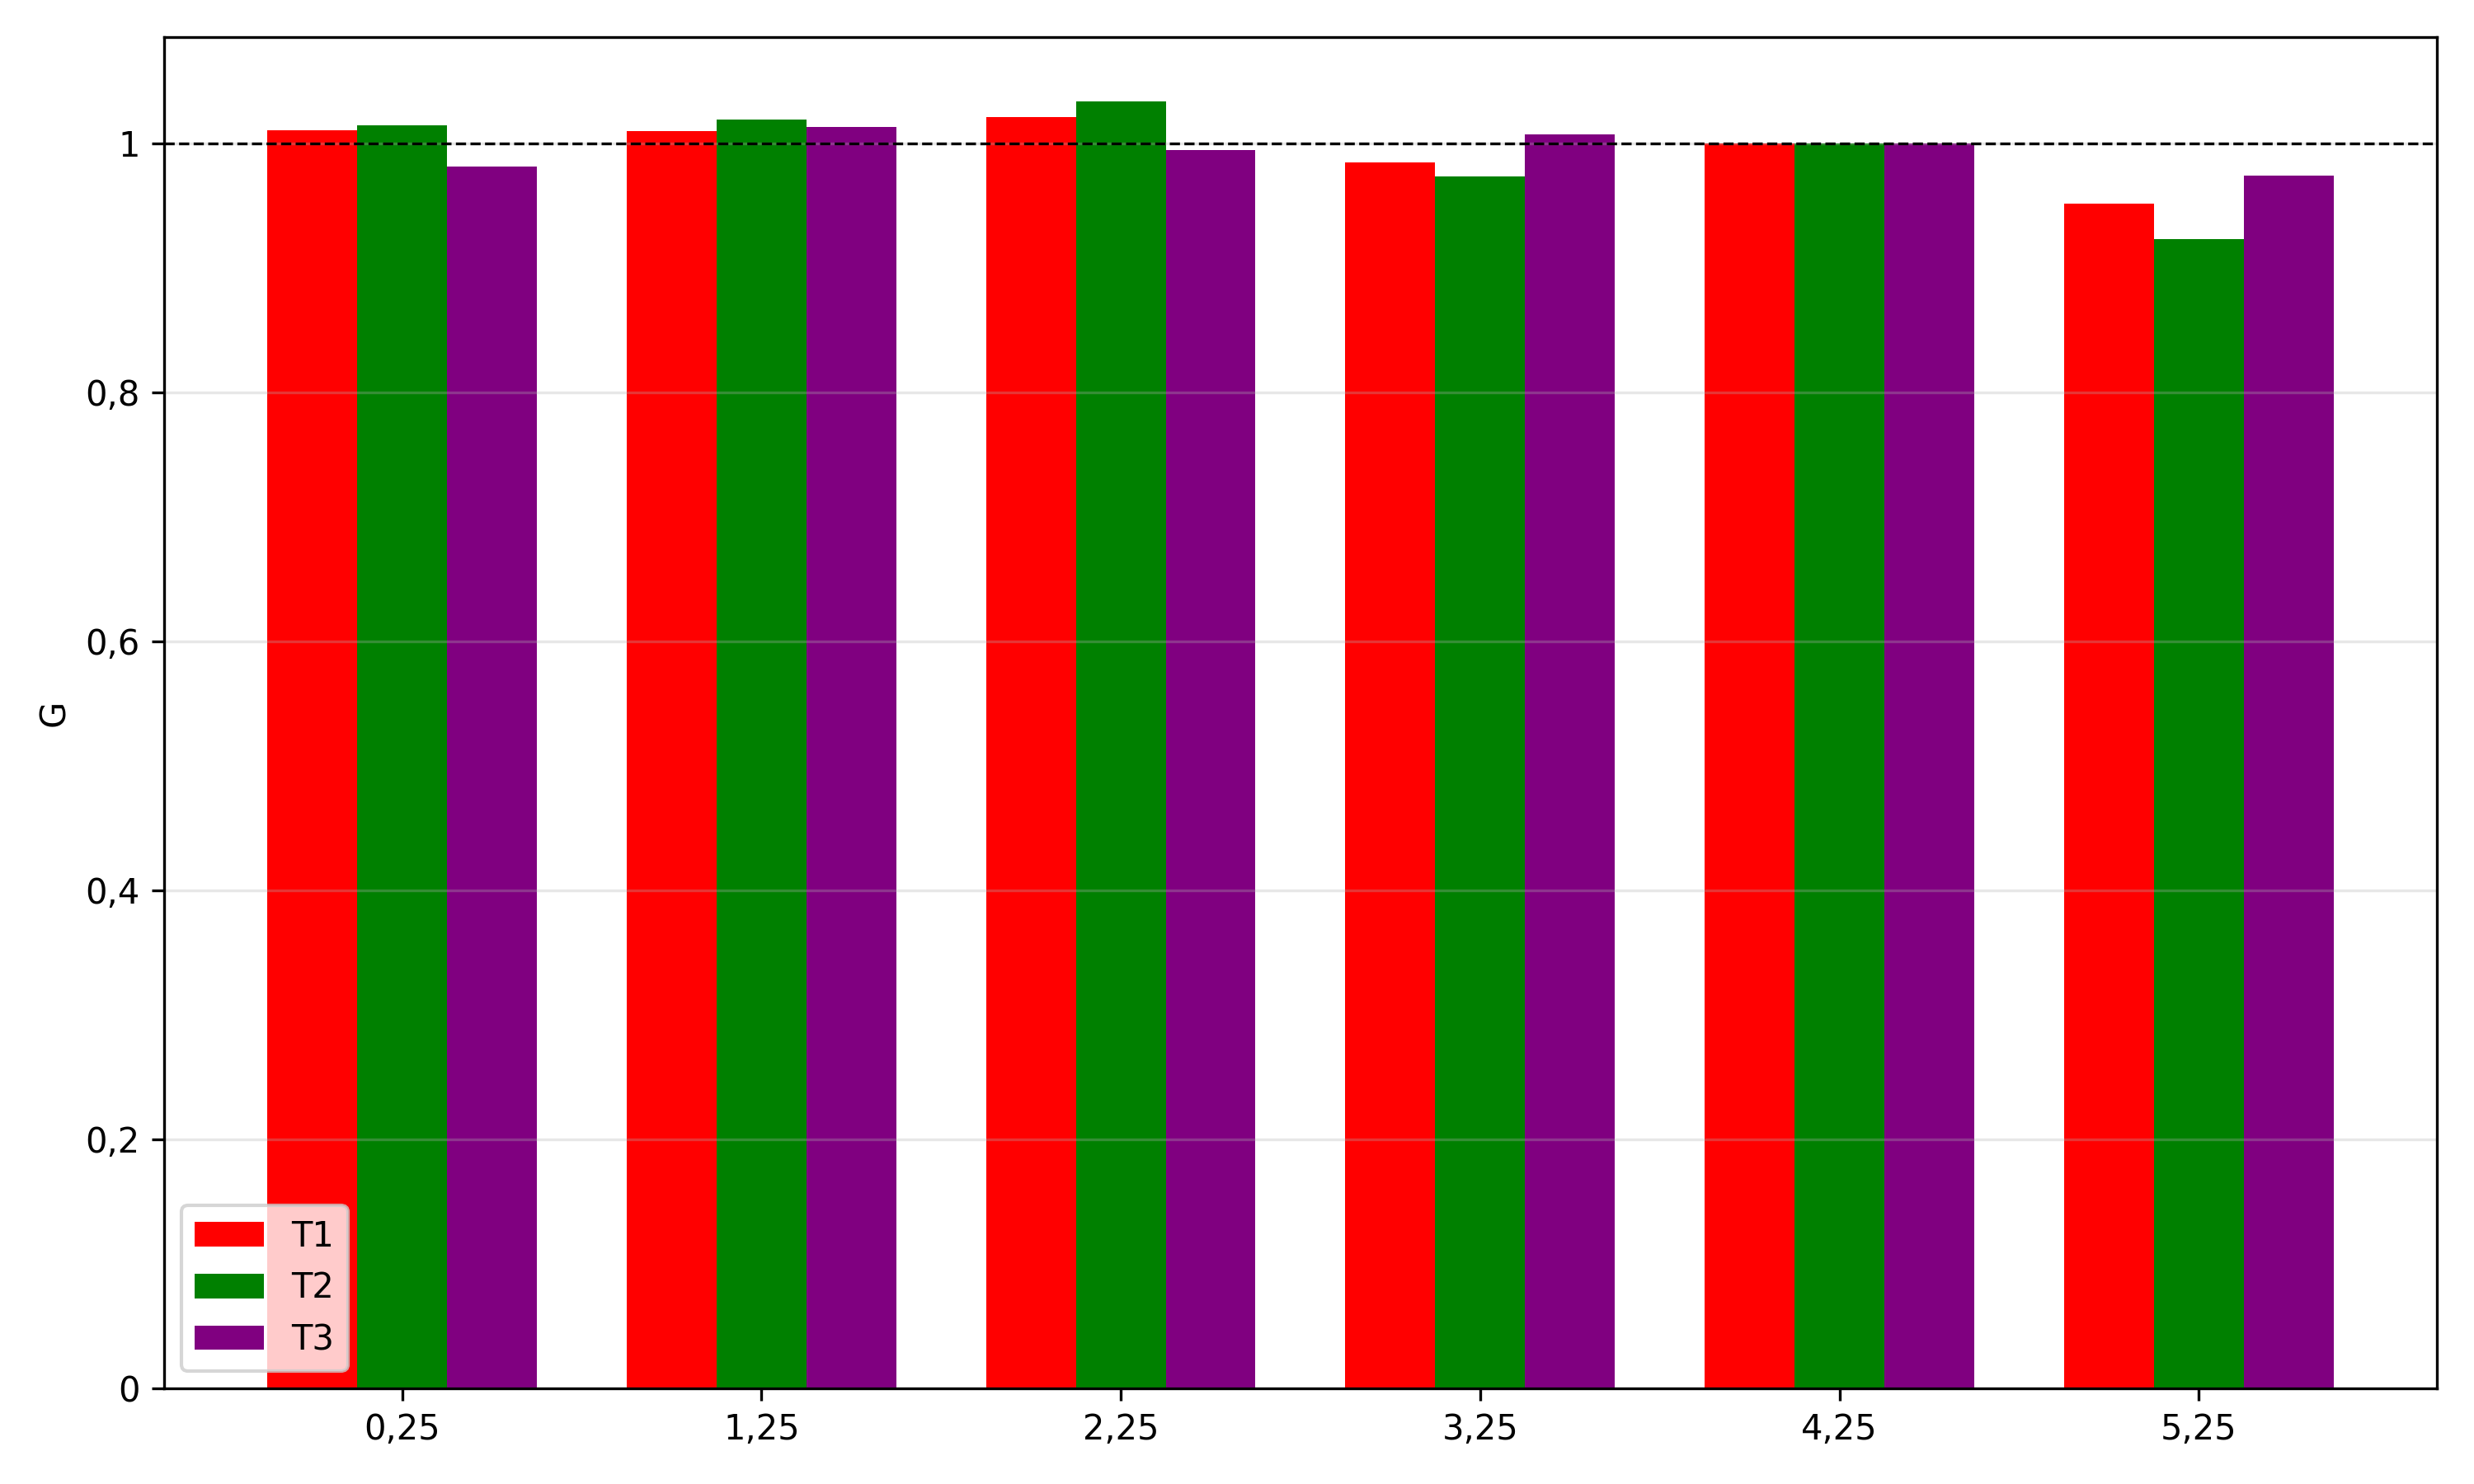
\includegraphics[width=\textwidth,height=0.9\textheight,keepaspectratio]{figures/ch07/fig_7_3.png}
\caption{Нормированные показатели эффективности $G_W$, $G_{M_f}$,
  $G_{f_T}$, $G_Q$, $G_{p_{\max}}$ для конфигураций T1, T2, T3
  при $K_{\mathrm{nom}} = 2{,}0$. Пунктирная горизонталь $G = 1$~--
  уровень гладкого подшипника.}
\label{fig:thrust_gains}
\end{figure}

\FloatBarrier


\section{Влияние параметра клина на рабочие характеристики}

Параметрический расчёт выполнен для
$K \in \{1{,}5;\; 2{,}0;\; 2{,}5;\; 3{,}0;\; 3{,}5;\; 4{,}0\}$.

\textit{Несущая сила.}
Несущая сила~$W$ имеет максимум при $K \approx 2{,}5$ для всех
вариантов (рисунок~\ref{fig:thrust_W_vs_K})~-- классическая
особенность клинового подшипника: при малых~$K$ клин слаб,
при больших~$K$ зазор~$h_{\mathrm{in}}$ слишком велик и давление
падает. Конфигурация~T2 превышает гладкий вариант по всему
диапазону~$K$. Конфигурация~T3 уступает гладкому при всех~$K$.

\begin{figure}[!ht]
\centering
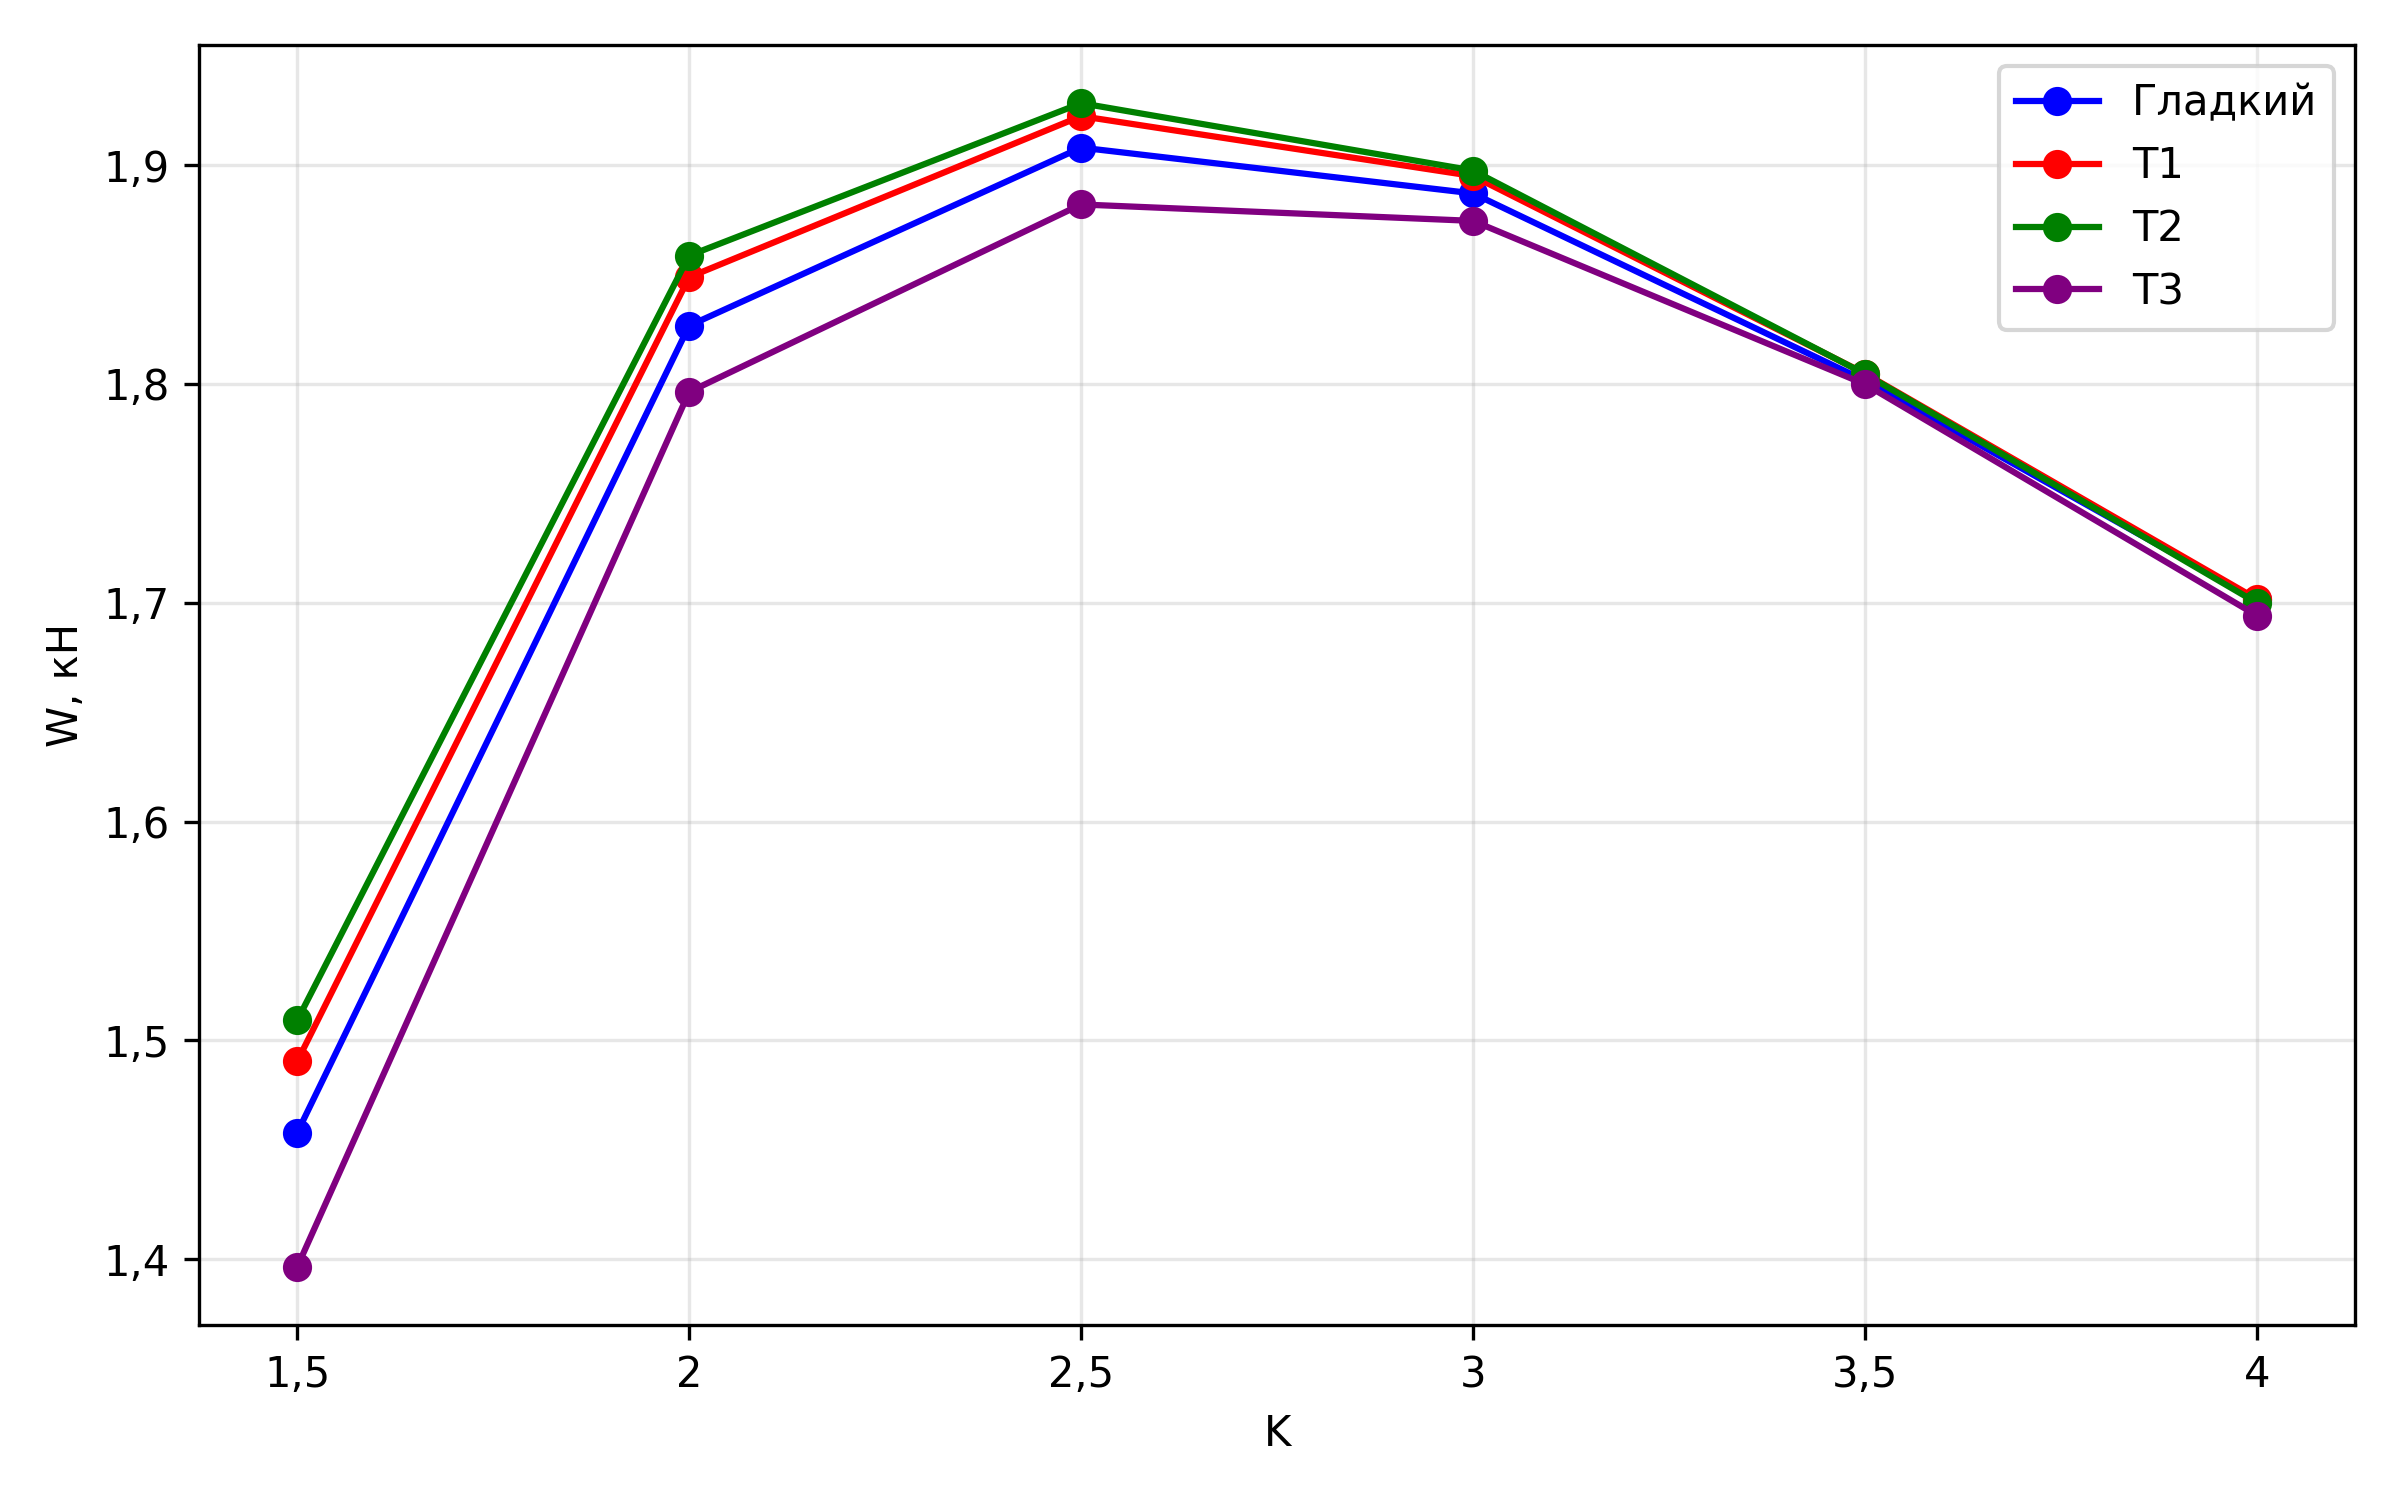
\includegraphics[width=\textwidth,height=0.9\textheight,keepaspectratio]{figures/ch07/fig_7_4.png}
\caption{Зависимость несущей силы $W$ от параметра клина $K$
  для гладкого подшипника и конфигураций T1, T2, T3.}
\label{fig:thrust_W_vs_K}
\end{figure}

\FloatBarrier

\textit{Коэффициент трения.}
Коэффициент трения~$f_T$ монотонно убывает с ростом~$K$
(рисунок~\ref{fig:thrust_fT_vs_K}). Конфигурация~T2 имеет
наименьший~$f_T$ при всех~$K$; конфигурация~T3 близка к гладкому
варианту или незначительно хуже.

\begin{figure}[!ht]
\centering
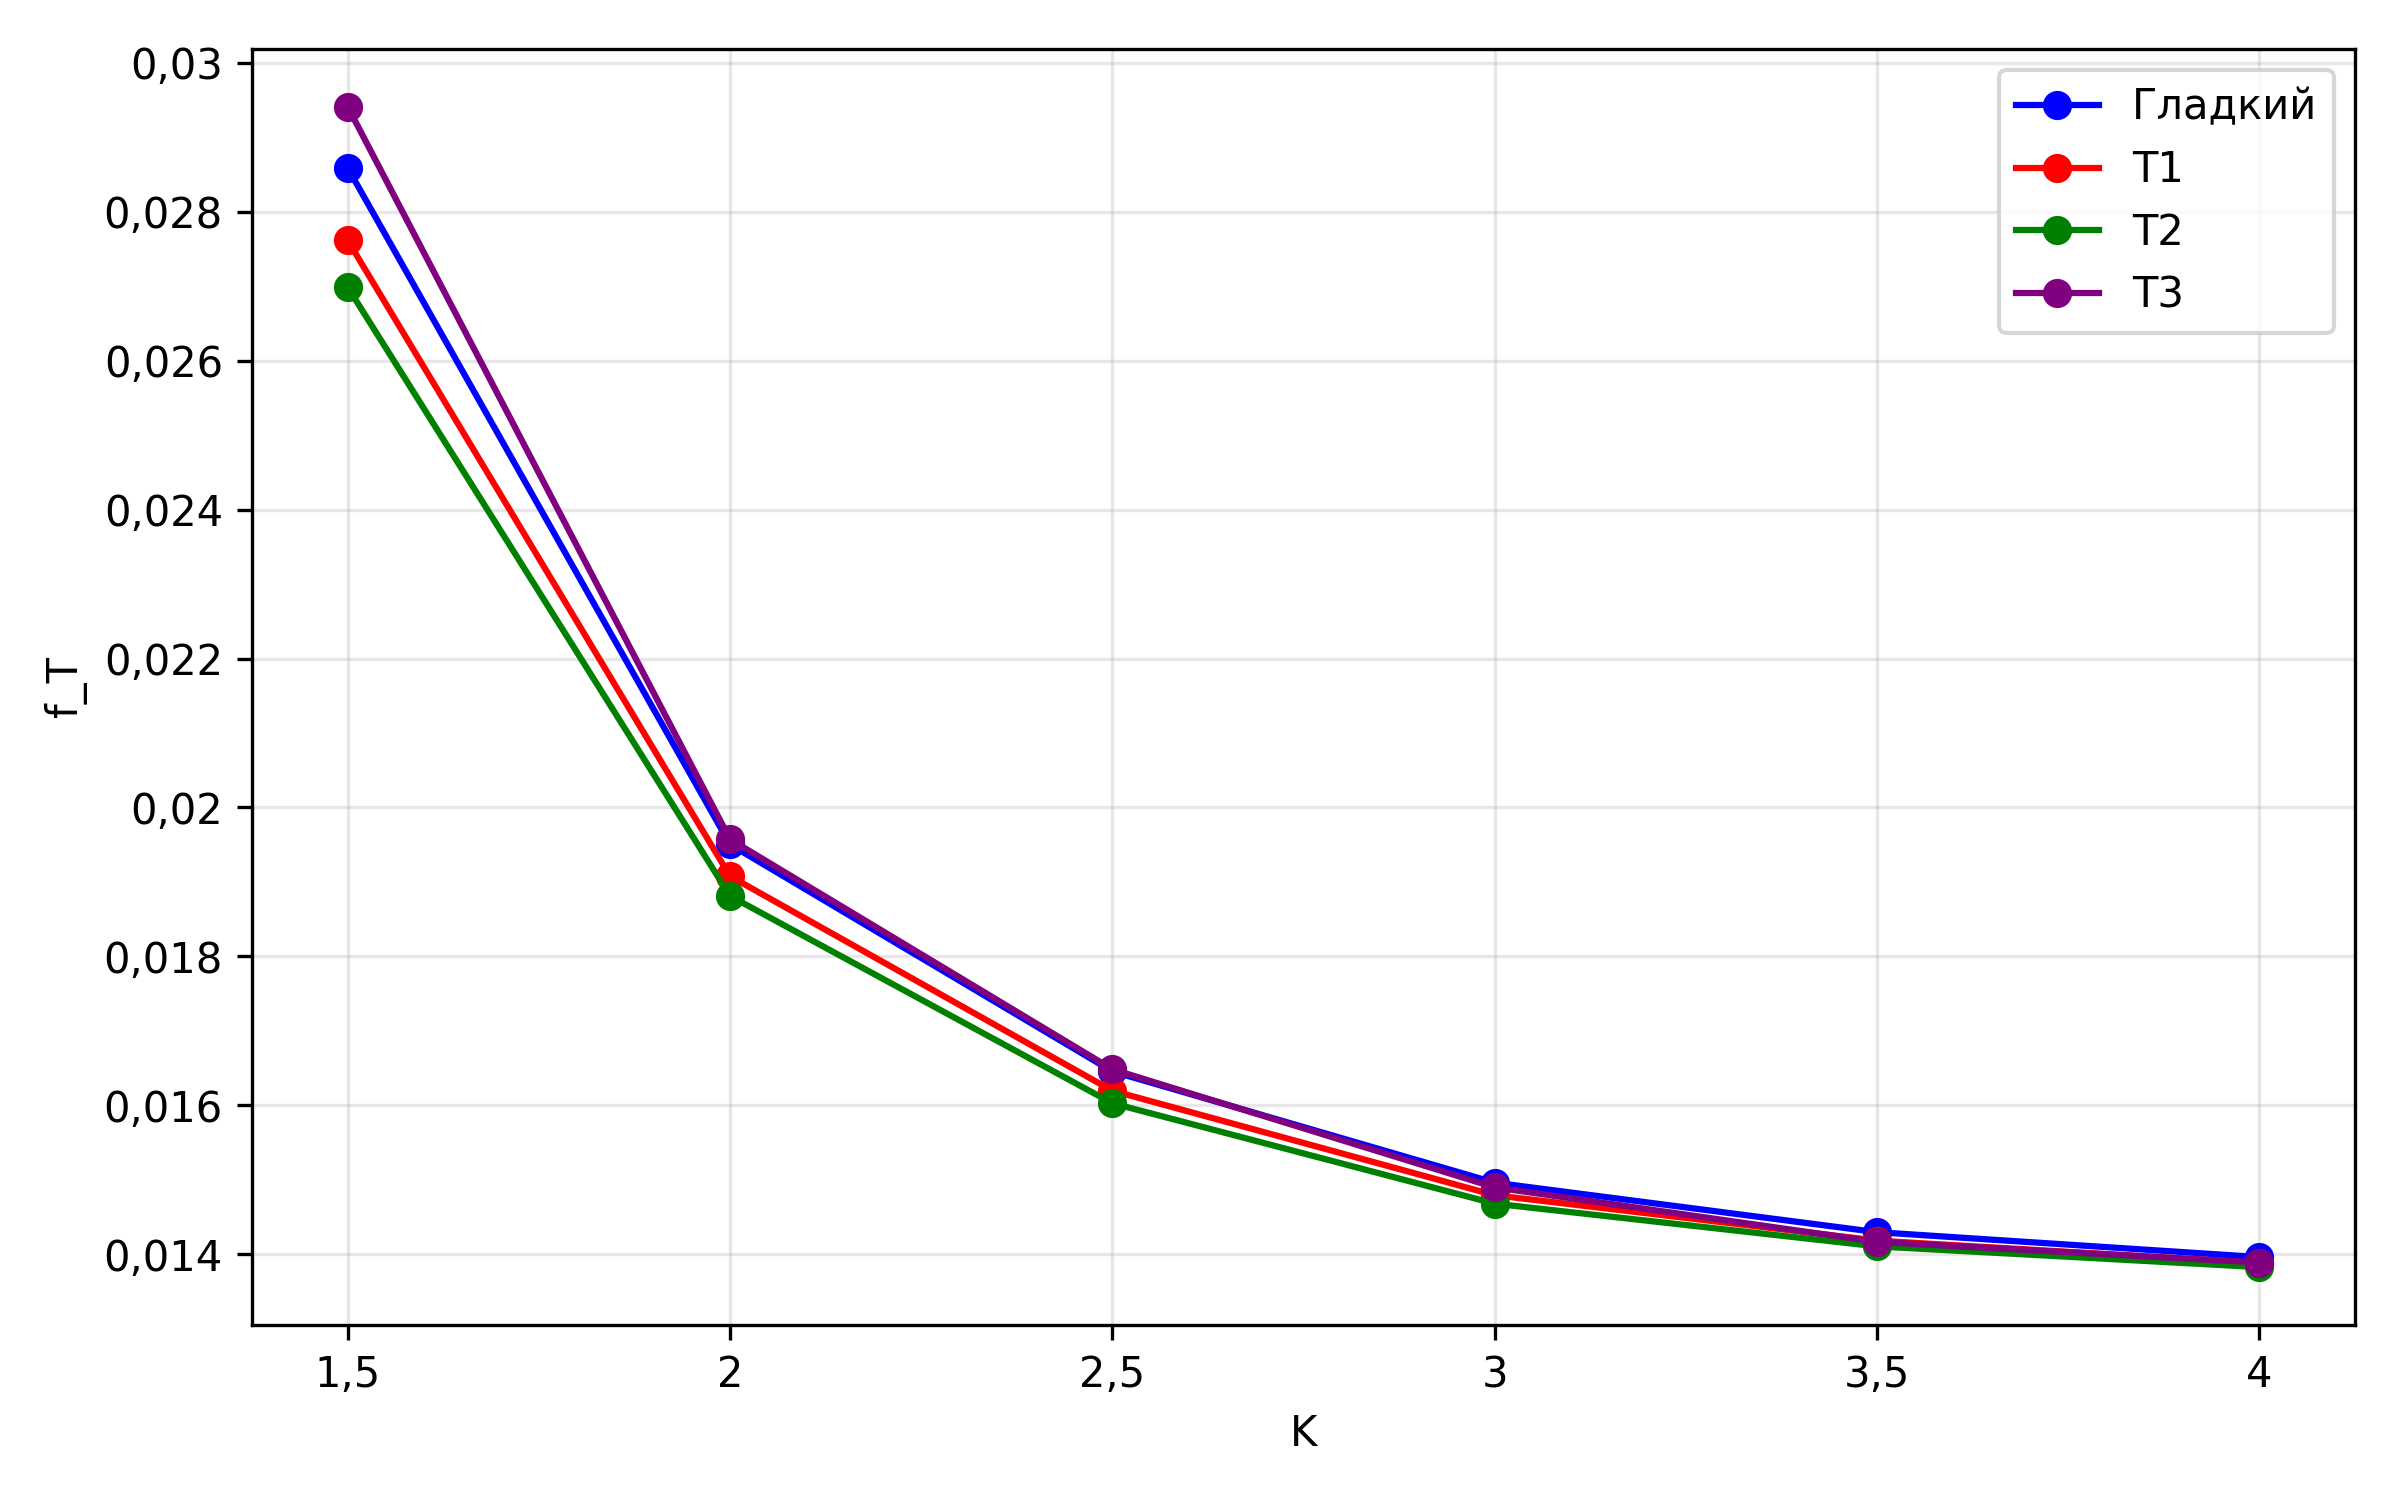
\includegraphics[width=\textwidth,height=0.9\textheight,keepaspectratio]{figures/ch07/fig_7_5.png}
\caption{Зависимость коэффициента трения $f_T$ от параметра
  клина $K$.}
\label{fig:thrust_fT_vs_K}
\end{figure}

\FloatBarrier

\textit{Расход смазочного материала.}
Расход~$Q$ монотонно растёт с~$K$
(рисунок~\ref{fig:thrust_Q_vs_K}). Различия между вариантами
невелики ($\leq 5\,\%$); конфигурация~T2 имеет несколько больший
расход вследствие увеличенного объёма лунок.

\begin{figure}[!ht]
\centering
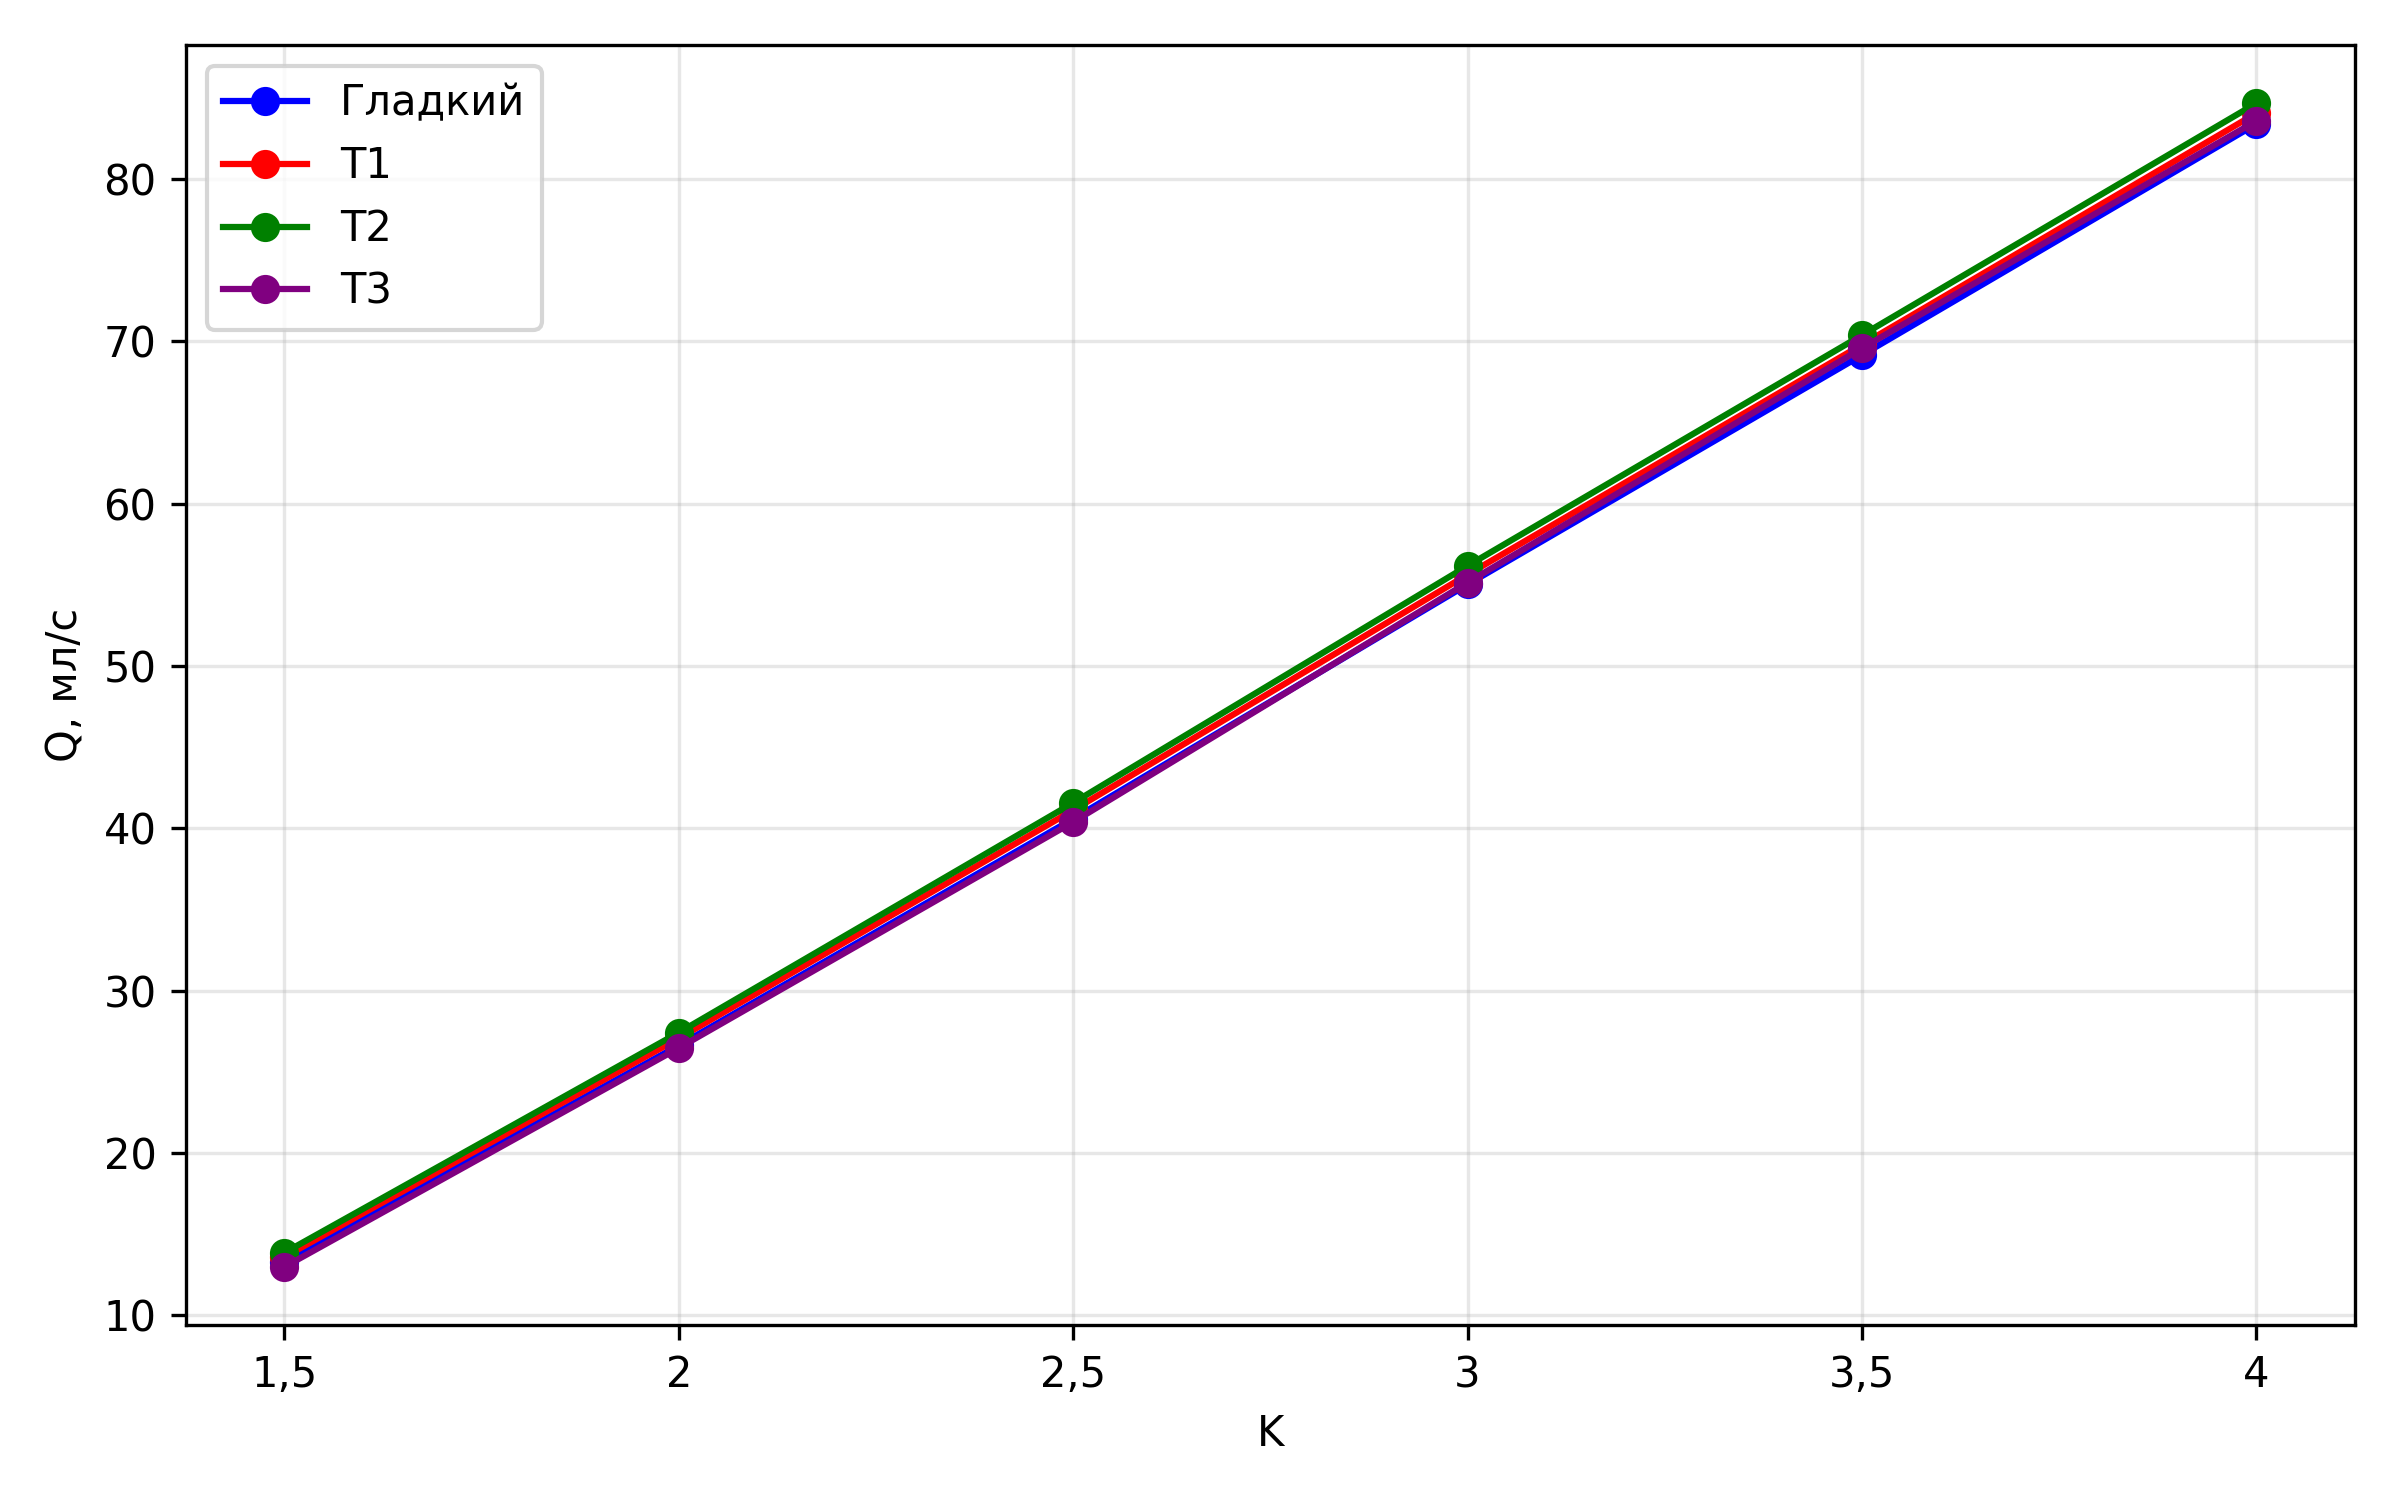
\includegraphics[width=\textwidth,height=0.9\textheight,keepaspectratio]{figures/ch07/fig_7_6.png}
\caption{Зависимость расхода смазки $Q$ от параметра клина $K$.}
\label{fig:thrust_Q_vs_K}
\end{figure}

\FloatBarrier

\textit{Максимальное давление.}
Максимальное давление~$p_{\max}$ растёт с~$K$ и достигает
насыщения при $K \approx 3$--$4$
(рисунок~\ref{fig:thrust_pmax_vs_K}). Конфигурации~T2 и~T1
демонстрируют более высокое~$p_{\max}$ по сравнению с гладким
вариантом; конфигурация~T3~-- ниже при малых~$K$ и выше
при больших~$K$.

\begin{figure}[!ht]
\centering
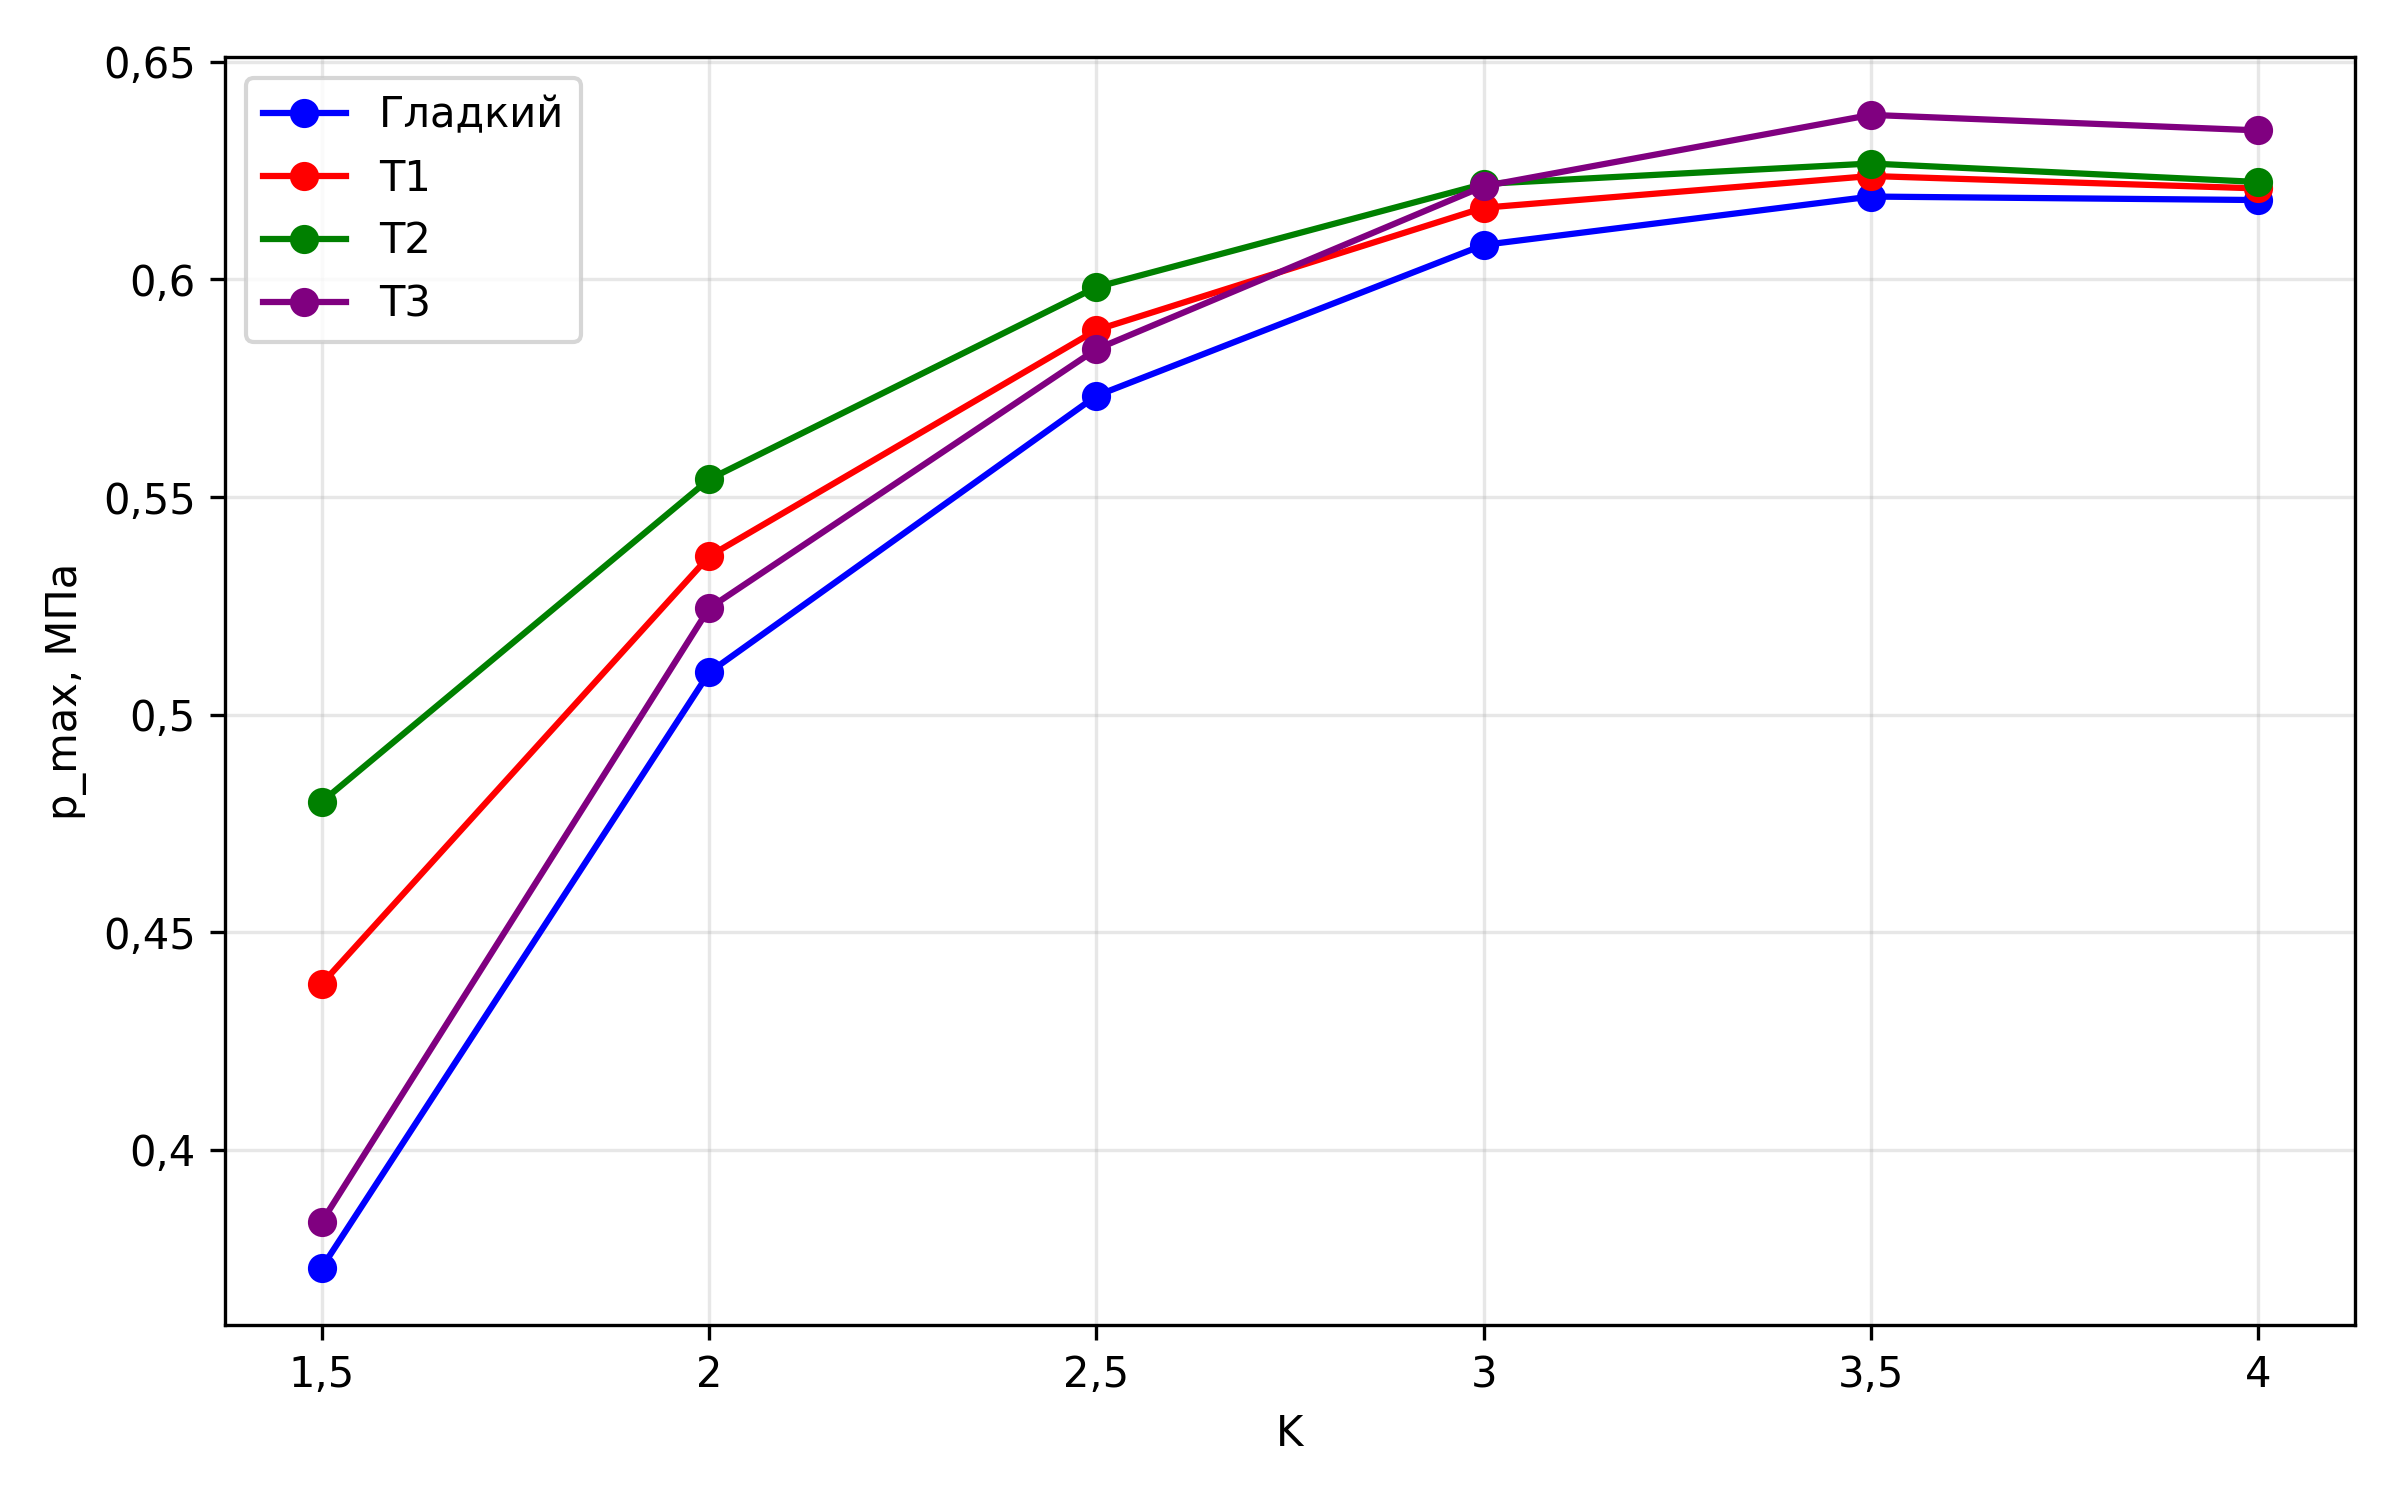
\includegraphics[width=\textwidth,height=0.9\textheight,keepaspectratio]{figures/ch07/fig_7_7.png}
\caption{Зависимость максимального давления $p_{\max}$ от параметра
  клина $K$.}
\label{fig:thrust_pmax_vs_K}
\end{figure}

\FloatBarrier

\textit{Минимальный зазор.}
В рассматриваемой постановке минимальный зазор определяется
выходной кромкой колодки:
$h_{\min} = h_{\mathrm{out}} = 50$~мкм для всех вариантов
и значений~$K$. Зависимость~$h_{\min}(K)$ не рассматривается.

\FloatBarrier


\section{Анализ распределения давления и обсуждение результатов}

\textit{Гладкий подшипник.}
Для гладкого подшипника поле давления $p(r, \theta)$ при
$K = 2{,}0$ имеет сглаженное распределение по радиусу
и единственный максимум в центральной части сектора
(рис.~\ref{fig:thrust_P3D_smooth}).
В рассматриваемой постановке при $K = 2{,}0$ во внутренней части
расчётной области не наблюдается выраженной области с нулевым
давлением; нулевые значения реализуются главным образом на
граничных кромках в соответствии с условиями~\eqref{eq:thrust_bc}.

\begin{figure}[!ht]
\centering
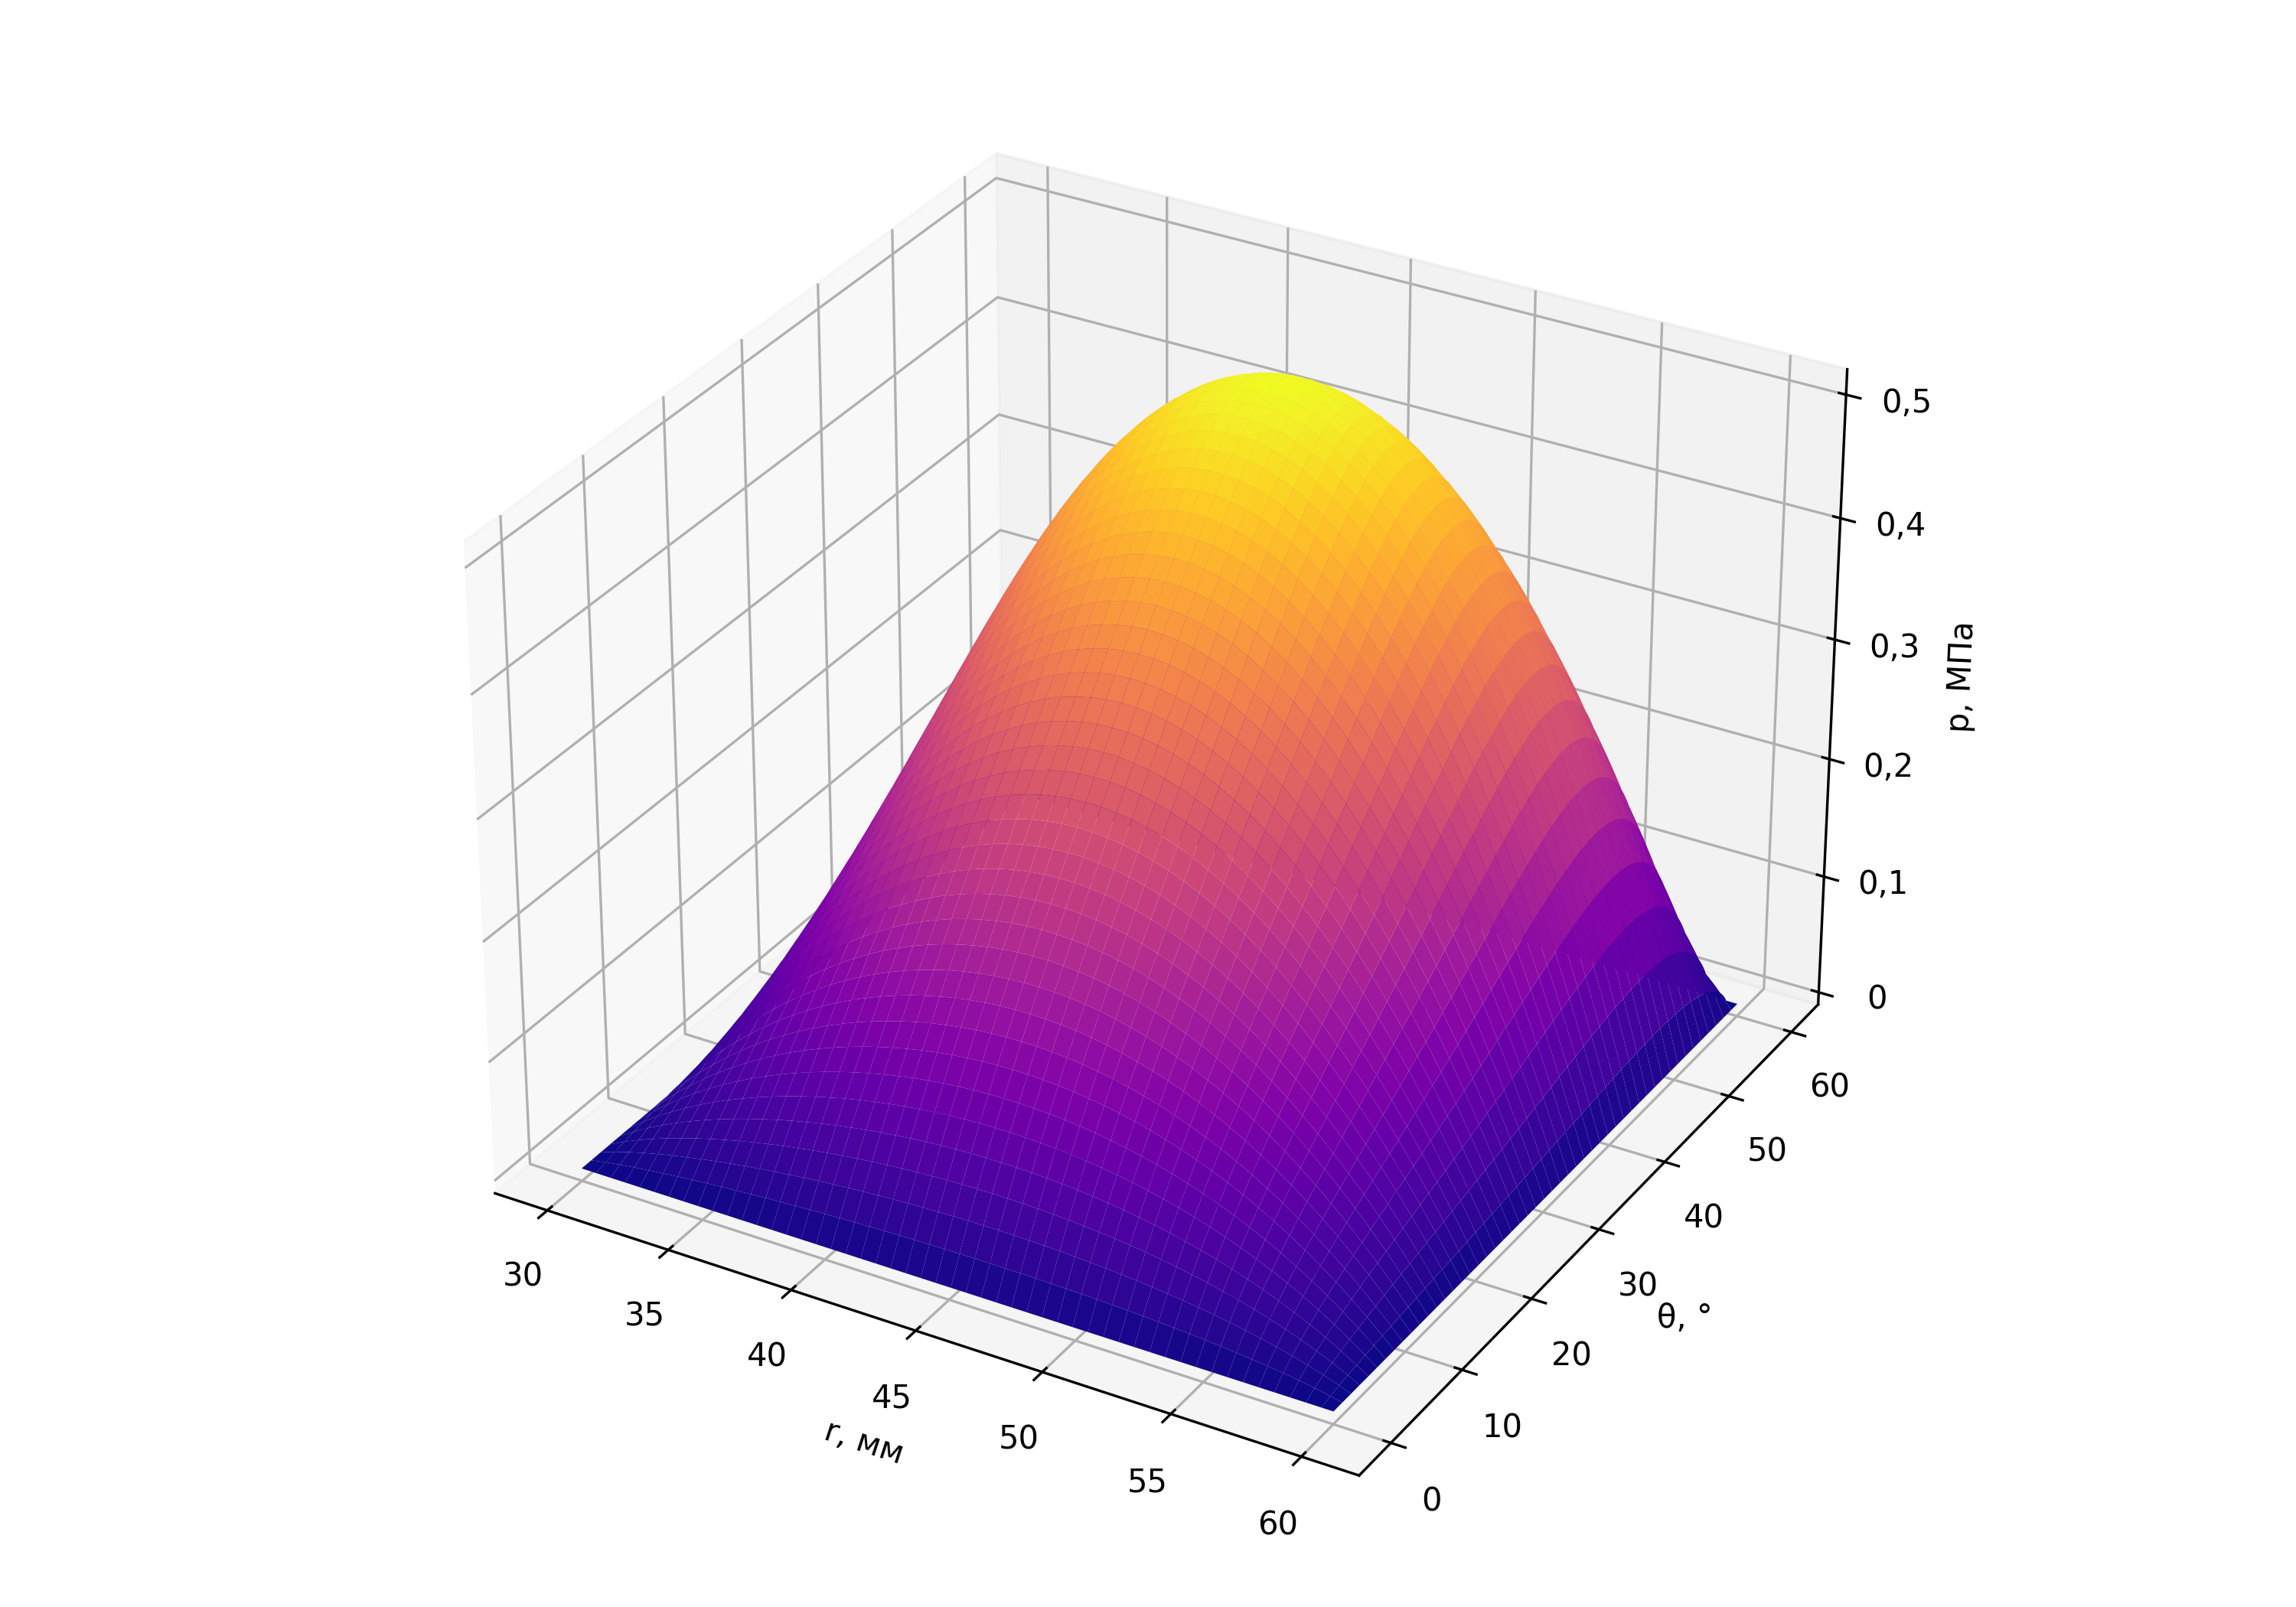
\includegraphics[width=\textwidth,height=0.9\textheight,keepaspectratio]{figures/ch07/fig_7_8.png}
\caption{Поле давления $p(r, \theta)$ гладкого подшипника
  при $K_{\mathrm{nom}} = 2{,}0$.}
\label{fig:thrust_P3D_smooth}
\end{figure}

\FloatBarrier

\textit{Конфигурация~T2.}
Текстурирование поверхности по конфигурации~T2 приводит к появлению
локальных пиков давления над лунками во входной и средней части
сектора (<<рябь>> на поверхности $p(r, \theta)$, рис.~\ref{fig:thrust_P3D_T2}). Интегральная
несущая сила возрастает вследствие дополнительных гидродинамических
клиньев, формируемых передними стенками лунок. В выходной части
сектора ($\theta > 0{,}7\beta$), свободной от текстуры, профиль
давления близок к гладкому случаю.

\begin{figure}[!ht]
\centering
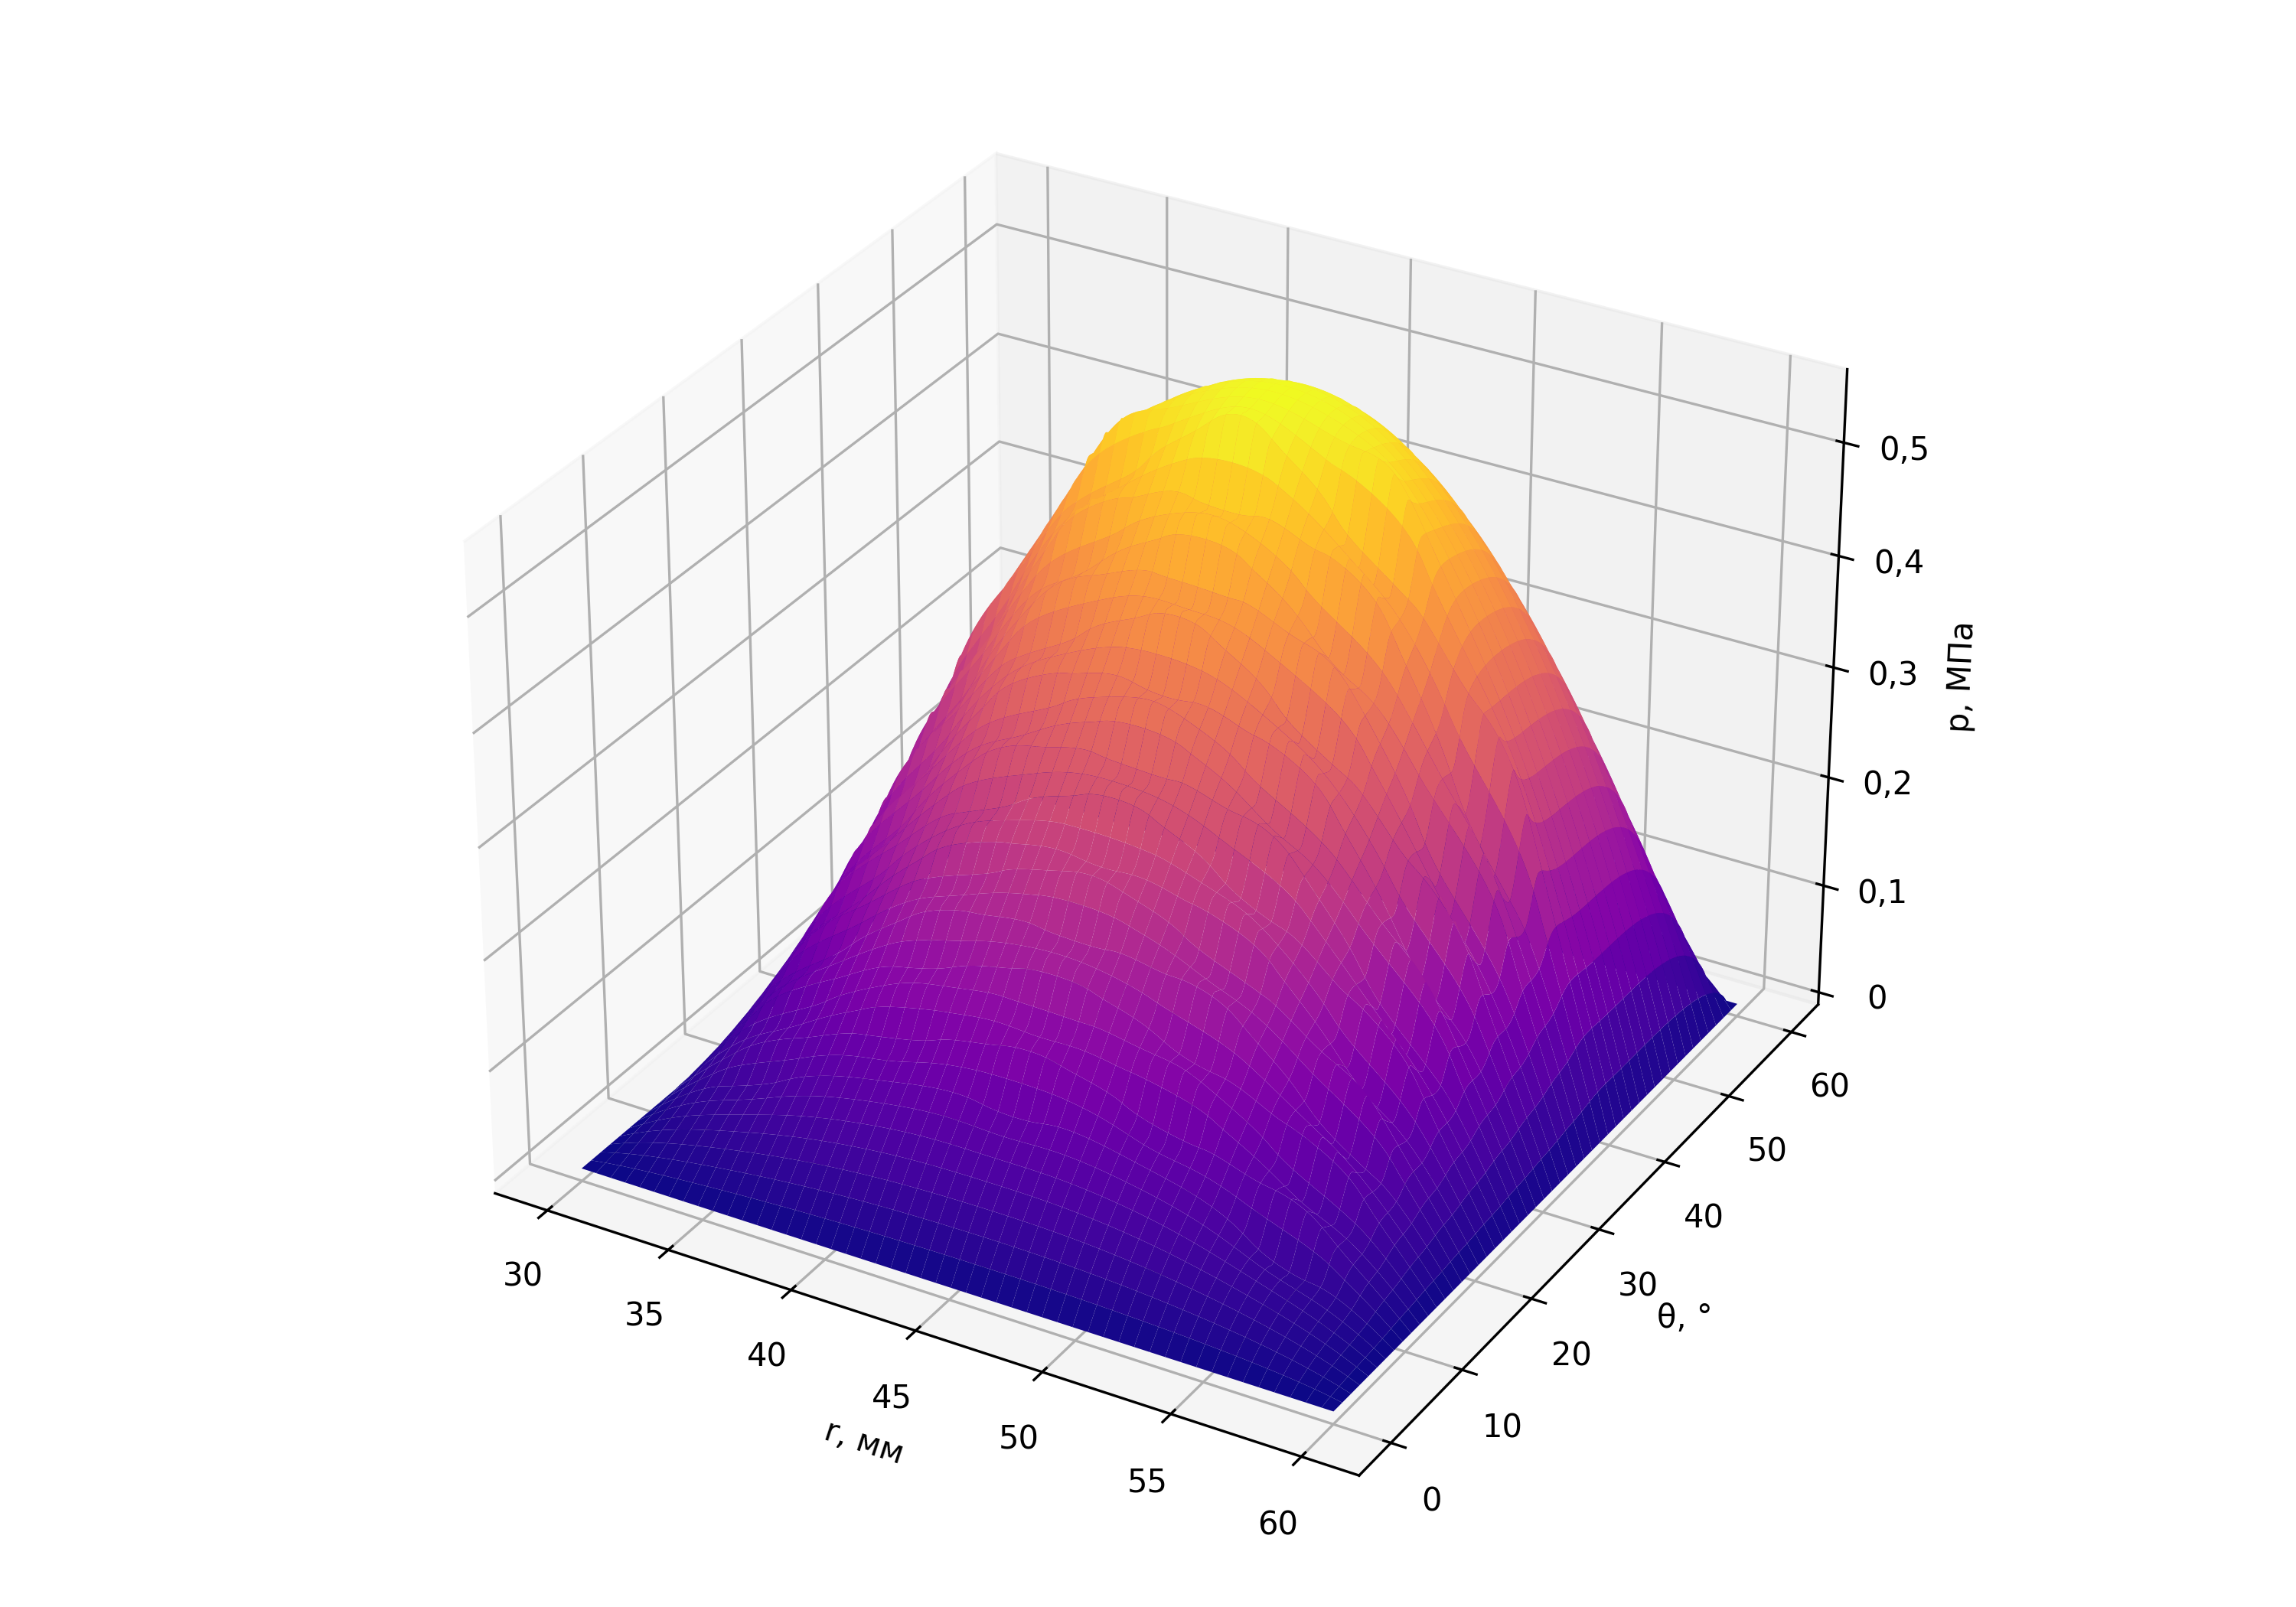
\includegraphics[width=\textwidth,height=0.9\textheight,keepaspectratio]{figures/ch07/fig_7_9.png}
\caption{Поле давления $p(r, \theta)$ для конфигурации~T2
  ($H_p = 0{,}40$, зона $0{,}1\beta$--$0{,}7\beta$)
  при $K_{\mathrm{nom}} = 2{,}0$.}
\label{fig:thrust_P3D_T2}
\end{figure}

\FloatBarrier

\textit{Конфигурация~T3.}
Конфигурация~T3 располагает лунки в средней и выходной части клина,
где зазор мал и давление убывает. В этой зоне передние стенки лунок
не создают эффективного гидродинамического клина; напротив, нарушение
плавности зазора в зоне убывающего давления снижает интегральную
несущую силу ниже уровня гладкого варианта ($G_W = 0{,}9816$).

\FloatBarrier
\section*{Выводы по главе~7}
\phantomsection\addcontentsline{toc}{section}{Выводы по главе~7}

Разработана численная модель упорного подшипника скольжения
с секторными колодками и детерминированными микроструктурами
рабочей поверхности~\cite{suh2015a,suh2015b,yang2021,song2024}. Модель основана на цилиндрической форме
уравнения Рейнольдса~\eqref{eq:thrust_reynolds}, решаемого
методом SOR на равномерной сетке $200 \times 300$ с обнулением
отрицательных давлений.

Проведён сравнительный расчёт гладкого варианта и конфигураций
T1, T2, T3 при $K_{\mathrm{nom}} = 2{,}0$. Установлено, что
текстурирование во входной и средней части клина (T1,~T2)
обеспечивает умеренный рост несущей способности и снижение
коэффициента трения. Наилучшие показатели у конфигурации~T2:
$G_W = 1{,}0145$, $G_{f_T} = 1{,}0337$.

Смещение текстуры в среднюю и выходную часть сектора (T3)
оказывается неэффективным: $G_W = 0{,}9816 < 1$, что подтверждает
определяющую роль зоны нанесения текстуры относительно зоны
нарастания давления.

Рост несущей способности при T1 и~T2 сопровождается увеличением
утечек смазочного материала ($G_Q = 0{,}9847$ и $0{,}9733$)
и максимального давления в плёнке ($G_{p_{\max}} = 0{,}9517$
и $0{,}9228$). Данный компромисс необходимо учитывать при выборе
конфигурации рабочей поверхности.

Параметрический расчёт по
$K \in [1{,}5;\; 4{,}0]$ показал, что несущая сила имеет максимум
при $K \approx 2{,}5$ для всех вариантов; коэффициент трения
монотонно убывает с ростом~$K$. Преимущество~T2 по несущей
способности сохраняется по всему исследованному диапазону~$K$.

Результаты анализа упорного подшипника дополняют результаты
глав~5 и~6, расширяя область применения детерминированных
микроструктур на подшипники с клиновым зазором.

       % Глава 5: Курсовое проектирование (НОВАЯ)
% % =============================================================
% 8 Анализ динамики роторной системы на подшипниках скольжения
%   с микроструктурами поверхности
% =============================================================
\chapter{Анализ динамики роторной системы на подшипниках скольжения с микроструктурами поверхности}

\section{Объект исследования и постановка задачи}

В главах~5 и~6 исследовалась стационарная несущая способность
радиального подшипника скольжения при наличии детерминированных
микроструктур рабочей поверхности. Настоящая глава посвящена
анализу динамического поведения системы «ротор~-- подшипник»
при наличии детерминированных микроструктур рабочей поверхности~\cite{miraskari2018a,miraskari2018b,muszynska1988}.
Исследуется тот же радиальный подшипник насоса (глава~5):
$R = 35$~мм, $c = 50$~мкм, $L = 56$~мм, $n = 2980$~об/мин.

Цель~-- оценить влияние текстуры~T2 (конфигурация с наилучшими
статическими характеристиками по результатам главы~5)
на коэффициенты динамической жёсткости, демпфирования, линейную
устойчивость и характер движения ротора в сравнении с гладким
подшипником~\cite{goodwin1997,jang1999,sayed2022}. Анализ выполнен в линейном приближении; основные выводы
формулируются для диапазона $\varepsilon = 0{,}2$--$0{,}6$.
Точка $\varepsilon = 0{,}8$ приводится на рисунках как
дополнительное качественное наблюдение.

Основные параметры модели сведены в таблицу~\ref{tab:dyn_params}.

\begin{table}[!ht]
\centering
\caption{Параметры динамической модели системы «ротор~-- подшипник»}
\label{tab:dyn_params}
\begin{tabularx}{\textwidth}{|X|c|c|c|}
\hline
\multicolumn{1}{|c|}{\textbf{Параметр}} & \textbf{Обозначение} & \textbf{Значение} & \textbf{Единица} \\
\hline
Радиус цапфы            & $R$        & 35{,}0   & мм \\
\hline
Длина подшипника        & $L$        & 56{,}0   & мм \\
\hline
Радиальный зазор        & $c$        & 50       & мкм \\
\hline
Динамическая вязкость   & $\mu$      & 0{,}01105 & Па$\cdot$с \\
\hline
Частота вращения        & $n$        & 2980     & об/мин \\
\hline
Угловая скорость        & $\omega$   & 311{,}9  & рад/с \\
\hline
Масса ротора            & $m$        & 10{,}0   & кг \\
\hline
Масса дисбаланса        & $m_u$      & 1{,}0    & г \\
\hline
Эксцентриситет дисбаланса & $e_u$    & 1{,}0    & мм \\
\hline
Диапазон $\varepsilon$  & --         & 0{,}2--0{,}6 & -- \\
\hline
\end{tabularx}
\end{table}


\section{Расчётная схема и принятые допущения}

Расчёт выполняется в системе координат $x$, $y$, связанной
с подшипником; ось~$x$ направлена по внешней нагрузке. Функция
смазочного зазора:
\begin{equation}
  h(\varphi, z, t) = c + x(t)\cos\varphi + y(t)\sin\varphi
    + h_{\mathrm{tex}}(\varphi, z).
  \label{eq:dyn_h}
\end{equation}
Данное выражение является единым для всех расчётов~-- статики,
динамики, вычисления сил и коэффициентов. Слагаемое
$h_{\mathrm{tex}}$ описывает эллипсоидальные лунки
конфигурации~T2 (подраздел~5.4).

Рабочая точка $(x_0,\, y_0)$ задаётся параметрически через
эксцентриситет: $x_0 = \varepsilon c$, $y_0 = 0$. Поиск
равновесия из уравнения баланса сил в данной главе не
выполняется; малые возмущения $\xi(t)$, $\eta(t)$
рассматриваются относительно заданной точки.

Модель принята изотермической ($T = T_0$,
$\mu = \mathrm{const}$); нелинейное нестационарное
пересчитывание поля давления на каждом шаге не выполняется.
Анализ ограничен линейной моделью малых возмущений.


\section{Математическая модель динамического смазочного слоя}

\textit{Статическое уравнение Рейнольдса.}
Безразмерная форма стационарного уравнения Рейнольдса
(глава~2, формула~\eqref{eq:reynolds_nondim}) для радиального
подшипника записывается в виде:
\begin{equation}
  \frac{\partial}{\partial\varphi}\!\left[H^3\,
    \frac{\partial P}{\partial\varphi}\right]
  + \left(\frac{R}{L}\right)^{\!2}
    \frac{\partial}{\partial Z}\!\left[H^3\,
    \frac{\partial P}{\partial Z}\right]
  = \frac{\partial H}{\partial\varphi}.
  \label{eq:dyn_reynolds_stat}
\end{equation}

\textit{Динамическое уравнение Рейнольдса.}
При учёте движения цапфы к правой части добавляется член сжатия
(squeeze-term), обусловленный производной зазора по времени:
\begin{equation}
  \frac{\partial}{\partial\varphi}\!\left[H^3\,
    \frac{\partial P}{\partial\varphi}\right]
  + \left(\frac{R}{L}\right)^{\!2}
    \frac{\partial}{\partial Z}\!\left[H^3\,
    \frac{\partial P}{\partial Z}\right]
  = \frac{\partial H}{\partial\varphi}
    + \frac{2R}{U}\,\frac{\partial H}{\partial t}.
  \label{eq:dyn_reynolds_dyn}
\end{equation}
Производная зазора по времени выводится из функции
зазора~\eqref{eq:dyn_h}:
\begin{equation}
  \frac{\partial h}{\partial t}
    = \dot{x}\cos\varphi + \dot{y}\sin\varphi.
  \label{eq:dyn_squeeze}
\end{equation}
Никаких дополнительных слагаемых, кроме следующих
из~\eqref{eq:dyn_h}, не вводится.

Граничные условия: периодичность по~$\varphi$; $P = 0$ при
$Z = \pm 1$; $P \geq 0$ (кавитация по условию Рейнольдса).

\textit{Гидродинамические силы.}
Компоненты силы, действующей на цапфу со стороны смазочного слоя,
вычисляются интегрированием поля давления:
\begin{align}
  F_x &= -\iint P\cos\varphi\,\mathrm{d}\varphi\,\mathrm{d}Z
    \cdot F_{\mathrm{scale}},
  \label{eq:dyn_Fx} \\
  F_y &= -\iint P\sin\varphi\,\mathrm{d}\varphi\,\mathrm{d}Z
    \cdot F_{\mathrm{scale}},
  \label{eq:dyn_Fy}
\end{align}
где $F_{\mathrm{scale}} = p_0 R L / 2$,\;
$p_0 = 6\mu U R / c^2$.

\textit{Коэффициенты жёсткости и демпфирования.}
Коэффициенты линейной модели определяются через частные
производные сил по координатам и скоростям:
\begin{equation}
  K_{xx} = -\frac{\partial F_x}{\partial x},\quad
  K_{xy} = -\frac{\partial F_x}{\partial y},\quad
  K_{yx} = -\frac{\partial F_y}{\partial x},\quad
  K_{yy} = -\frac{\partial F_y}{\partial y},
  \label{eq:dyn_K}
\end{equation}
\begin{equation}
  C_{xx} = -\frac{\partial F_x}{\partial\dot{x}},\quad
  C_{xy} = -\frac{\partial F_x}{\partial\dot{y}},\quad
  C_{yx} = -\frac{\partial F_y}{\partial\dot{x}},\quad
  C_{yy} = -\frac{\partial F_y}{\partial\dot{y}}.
  \label{eq:dyn_C}
\end{equation}
Жёсткости вычисляются через статический solver,
демпфирование~-- через динамический solver. Все производные~--
вокруг одной и той же точки $(x_0,\, y_0)$. Ручная коррекция
знаков не применяется.

\textit{Модель ротора.}
Уравнения движения для малых возмущений
$\xi = x - x_0$, $\eta = y - y_0$:
\begin{align}
  m\ddot{\xi} + C_{xx}\dot{\xi} + C_{xy}\dot{\eta}
    + K_{xx}\xi + K_{xy}\eta &= F_{x,\mathrm{unb}}(t),
  \label{eq:dyn_ode_x} \\
  m\ddot{\eta} + C_{yx}\dot{\xi} + C_{yy}\dot{\eta}
    + K_{yx}\xi + K_{yy}\eta &= F_{y,\mathrm{unb}}(t).
  \label{eq:dyn_ode_y}
\end{align}
Сила дисбаланса:
\begin{equation}
  F_{x,\mathrm{unb}} = m_u e_u \omega^2 \cos(\omega t),\qquad
  F_{y,\mathrm{unb}} = m_u e_u \omega^2 \sin(\omega t).
  \label{eq:dyn_unbalance}
\end{equation}

Критерий устойчивости~-- максимальная вещественная часть
собственных значений матрицы состояния системы $4 \times 4$:
$\mathrm{Re}(\lambda_{\max}) < 0$~-- система устойчива.


\section{Численная реализация и верификация модели}

Расчётная область дискретизируется равномерной сеткой
$360 \times 120$ узлов по~$\varphi$ и~$Z$ (точка~$2\pi$
не дублируется). Статический solver~-- пакет
\texttt{reynolds\_solver} (глава~5); динамический solver
реализован отдельно с идентичной дискретизацией и добавленным
squeeze-term. Оба решателя используют метод SOR
с~$\omega_{\mathrm{SOR}} = 1{,}5$,
$\mathrm{TOL} = 10^{-5}$. Коэффициенты вычисляются
центральными разностями с шагами $\Delta x = 0{,}005c$,
$\Delta v = 0{,}005U$.

Для проверки численной устойчивости выполнены два контрольных
расчёта при $\varepsilon = 0{,}6$: шаг конечных разностей
уменьшен вдвое ($\Delta x \to \Delta x/2$,
$\Delta v \to \Delta v/2$) и сетка увеличена до
$480 \times 160$. Результаты верификации для гладкого подшипника как базового
варианта сведены в таблицу~\ref{tab:dyn_verif}.

\begin{table}[!ht]
\centering
\caption{Верификация численной устойчивости при $\varepsilon = 0{,}6$
  (гладкий подшипник)}
\label{tab:dyn_verif}
\small
\begin{tabular}{|l|c|c|c|c|}
\hline
\textbf{Показатель}
  & $\mathbf{360 \times 120}$\textbf{,}
  & $\mathbf{360 \times 120}$\textbf{,}
  & $\mathbf{480 \times 160}$\textbf{,}
  & \textbf{Откл. при} \\
  & $\boldsymbol{\Delta x{,}\,\Delta v}$\textbf{ ном.}
  & $\boldsymbol{\Delta x/2{,}\,\Delta v/2}$
  & $\boldsymbol{\Delta x{,}\,\Delta v}$\textbf{ ном.}
  & \textbf{сгущении сетки} \\
\hline
$K_{xx}$, $10^8$~Н/м & $3{,}51$ & $3{,}51$ & $3{,}52$ & 0{,}4 \\
\hline
$K_{yy}$, $10^8$~Н/м & $1{,}20$ & $1{,}20$ & $1{,}20$ & 0{,}0 \\
\hline
$K_{xy}$, $10^8$~Н/м & $1{,}26$ & $1{,}26$ & $1{,}26$ & 0{,}1 \\
\hline
$K_{yx}$, $10^8$~Н/м & $-1{,}84$ & $-1{,}84$ & $-1{,}85$ & 0{,}6 \\
\hline
$C_{xx}$, $10^6$~Н$\cdot$с/м & $2{,}57$ & $2{,}57$ & $2{,}57$ & 0{,}0 \\
\hline
$C_{yy}$, $10^6$~Н$\cdot$с/м & $1{,}08$ & $1{,}08$ & $1{,}08$ & 0{,}0 \\
\hline
$\mathrm{Re}_{\max}$ & $-122{,}3$ & $-121{,}7$ & $-122{,}6$ & $|\Delta| = 0{,}2$ \\
\hline
\end{tabular}
\end{table}

\FloatBarrier

Верификационные расчёты для гладкого подшипника при
$\varepsilon = 0{,}6$ показали, что коэффициенты жёсткости
$K_{ij}$ и прямые коэффициенты демпфирования $C_{xx}$, $C_{yy}$
слабо зависят от уменьшения шага конечного дифференцирования
и от сгущения сетки (отклонение менее~$1\,\%$). Для
текстурированного варианта~T2 в области больших эксцентриситетов
наблюдается более высокая чувствительность отдельных коэффициентов
жёсткости к разрешению сетки; однако качественные выводы о влиянии
текстуры сохраняются.
Перекрёстные коэффициенты демпфирования $C_{xy}$, $C_{yx}$
проявляют повышенную чувствительность к шагу $\Delta v$
и не используются в данной работе как количественный результат.


\section{Влияние эксцентриситета на коэффициенты жёсткости}

Прямые коэффициенты жёсткости $K_{xx}$ и $K_{yy}$ монотонно
возрастают с ростом~$\varepsilon$ для обоих вариантов
(рисунок~\ref{fig:dyn_K_direct}). На рисунках для полноты
сопоставления дополнительно приведена точка
$\varepsilon = 0{,}8$; основные количественные выводы настоящей
главы относятся к диапазону
$\varepsilon = 0{,}2$--$0{,}6$. Конфигурация~T2 обеспечивает
существенно более высокие значения $K_{xx}$ по всему диапазону:
при $\varepsilon = 0{,}6$ значение
$K_{xx}^{(T2)} = 6{,}25 \cdot 10^8$~Н/м против
$K_{xx}^{(\text{гл.})} = 3{,}51 \cdot 10^8$~Н/м, то есть
прирост составляет около~$78\,\%$. Коэффициент $K_{yy}$ у~T2
также выше и при $\varepsilon = 0{,}6$ составляет
$2{,}06 \cdot 10^8$~Н/м против $1{,}20 \cdot 10^8$~Н/м.

Перекрёстные коэффициенты $K_{xy} > 0$ и $K_{yx} < 0$
сохраняют свои знаки во всём основном диапазоне
$\varepsilon = 0{,}2$--$0{,}6$ для обоих вариантов
(рисунок~\ref{fig:dyn_K_cross}). Их значения для гладкого
и текстурированного подшипников сопоставимы по порядку величины;
конфигурация~T2 не приводит к принципиальному изменению характера
перекрёстной жёсткостной связи.

Сводные значения коэффициентов при $\varepsilon = 0{,}6$
приведены в таблице~\ref{tab:dyn_coeffs}.

\begin{table}[!ht]
\centering
\caption{Коэффициенты жёсткости, демпфирования и запас
  устойчивости при $\varepsilon = 0{,}6$}
\label{tab:dyn_coeffs}
\small
\begin{tabular}{|l|c|c|c|c|c|c|c|}
\hline
\textbf{Вариант}
  & $\boldsymbol{K_{xx}}$, & $\boldsymbol{K_{yy}}$,
  & $\boldsymbol{K_{xy}}$, & $\boldsymbol{K_{yx}}$,
  & $\boldsymbol{C_{xx}}$, & $\boldsymbol{C_{yy}}$,
  & $\boldsymbol{\mathrm{Re}_{\max}}$ \\
  & $10^8$~Н/м & $10^8$~Н/м
  & $10^8$~Н/м & $10^8$~Н/м
  & $10^6$~Н$\cdot$с/м & $10^6$~Н$\cdot$с/м
  & \\
\hline
Гладкий
  & $3{,}51$ & $1{,}20$ & $1{,}26$ & $-1{,}84$
  & $2{,}57$ & $1{,}08$
  & $-122{,}3$ \\
\hline
T2
  & $6{,}25$ & $2{,}06$ & $1{,}23$ & $-1{,}76$
  & $1{,}85$ & $0{,}90$
  & $-282{,}5$ \\
\hline
\end{tabular}
\end{table}

\FloatBarrier

Значение $\varepsilon = 0{,}6$ выбрано как характерный режим
с выраженным динамическим эффектом текстурирования. Для
конфигурации~T2 в данной точке наблюдается умеренная
чувствительность прямых коэффициентов жёсткости к разрешению
сетки, не меняющая качественных выводов.

\begin{figure}[!ht]
\centering
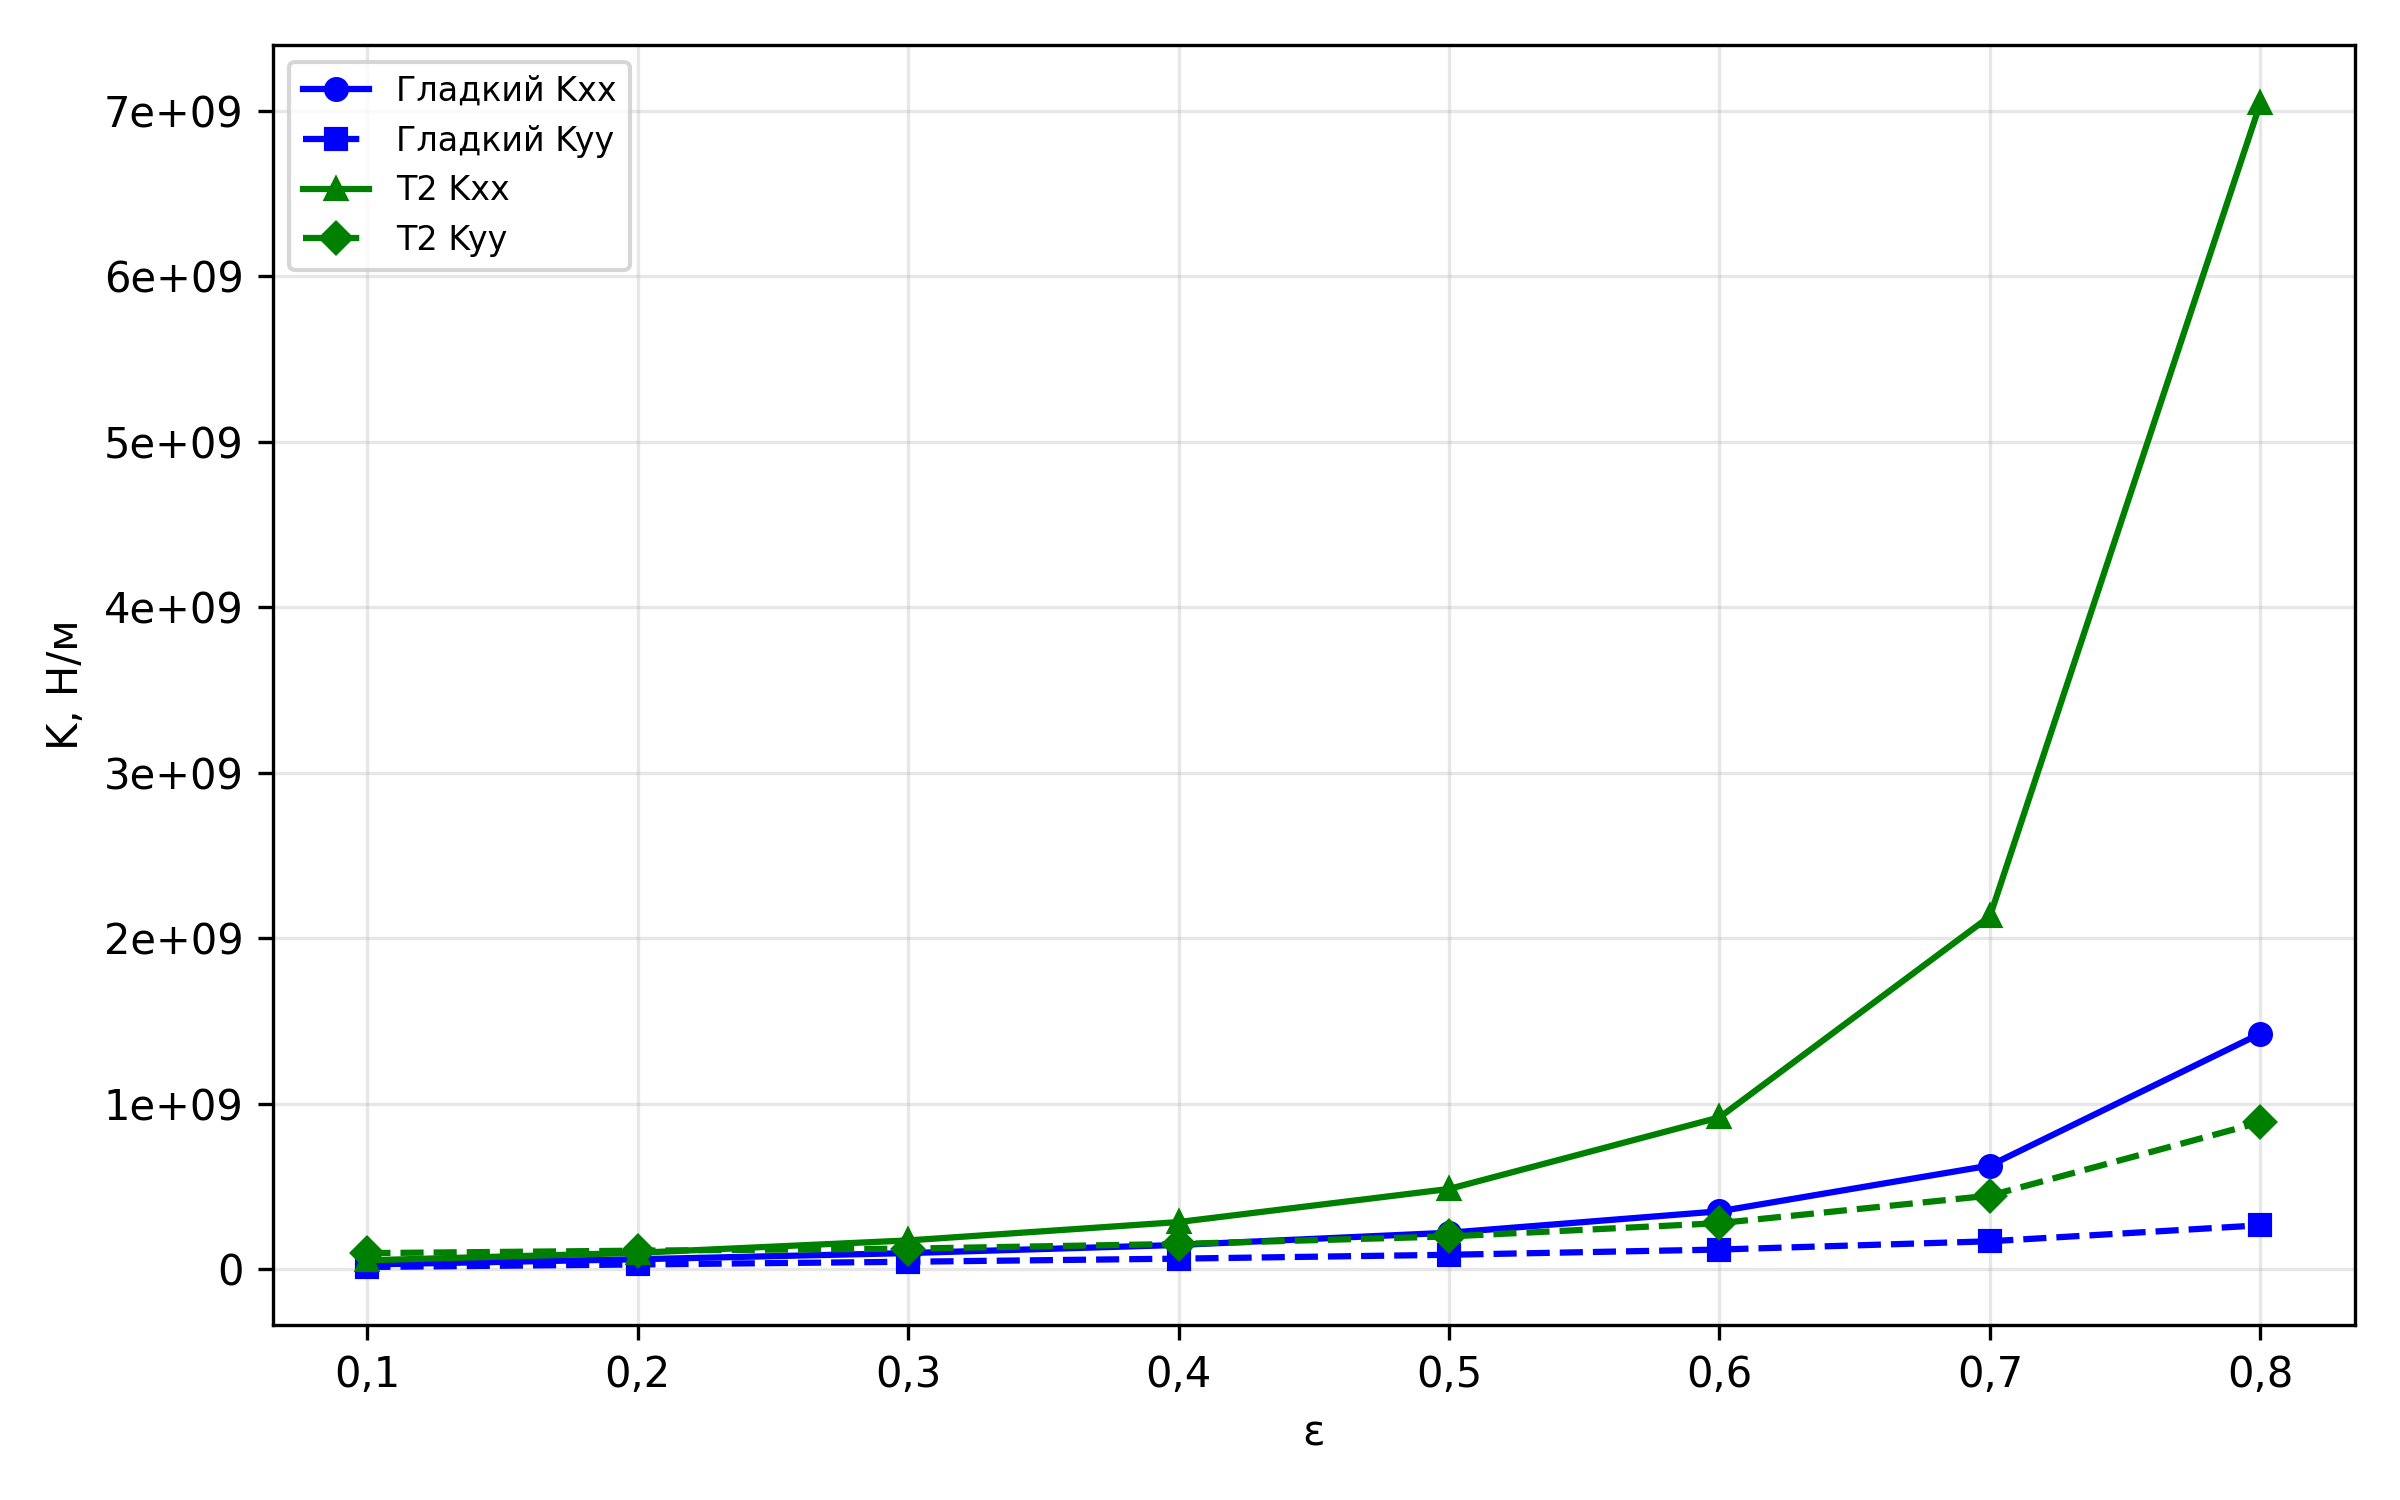
\includegraphics[width=\textwidth,height=0.9\textheight,keepaspectratio]{figures/ch08/fig_8_1.png}
\caption{Зависимость прямых коэффициентов жёсткости $K_{xx}$ и $K_{yy}$
  от относительного эксцентриситета~$\varepsilon$
  для гладкого подшипника и конфигурации~T2.}
\label{fig:dyn_K_direct}
\end{figure}

\begin{figure}[!ht]
\centering
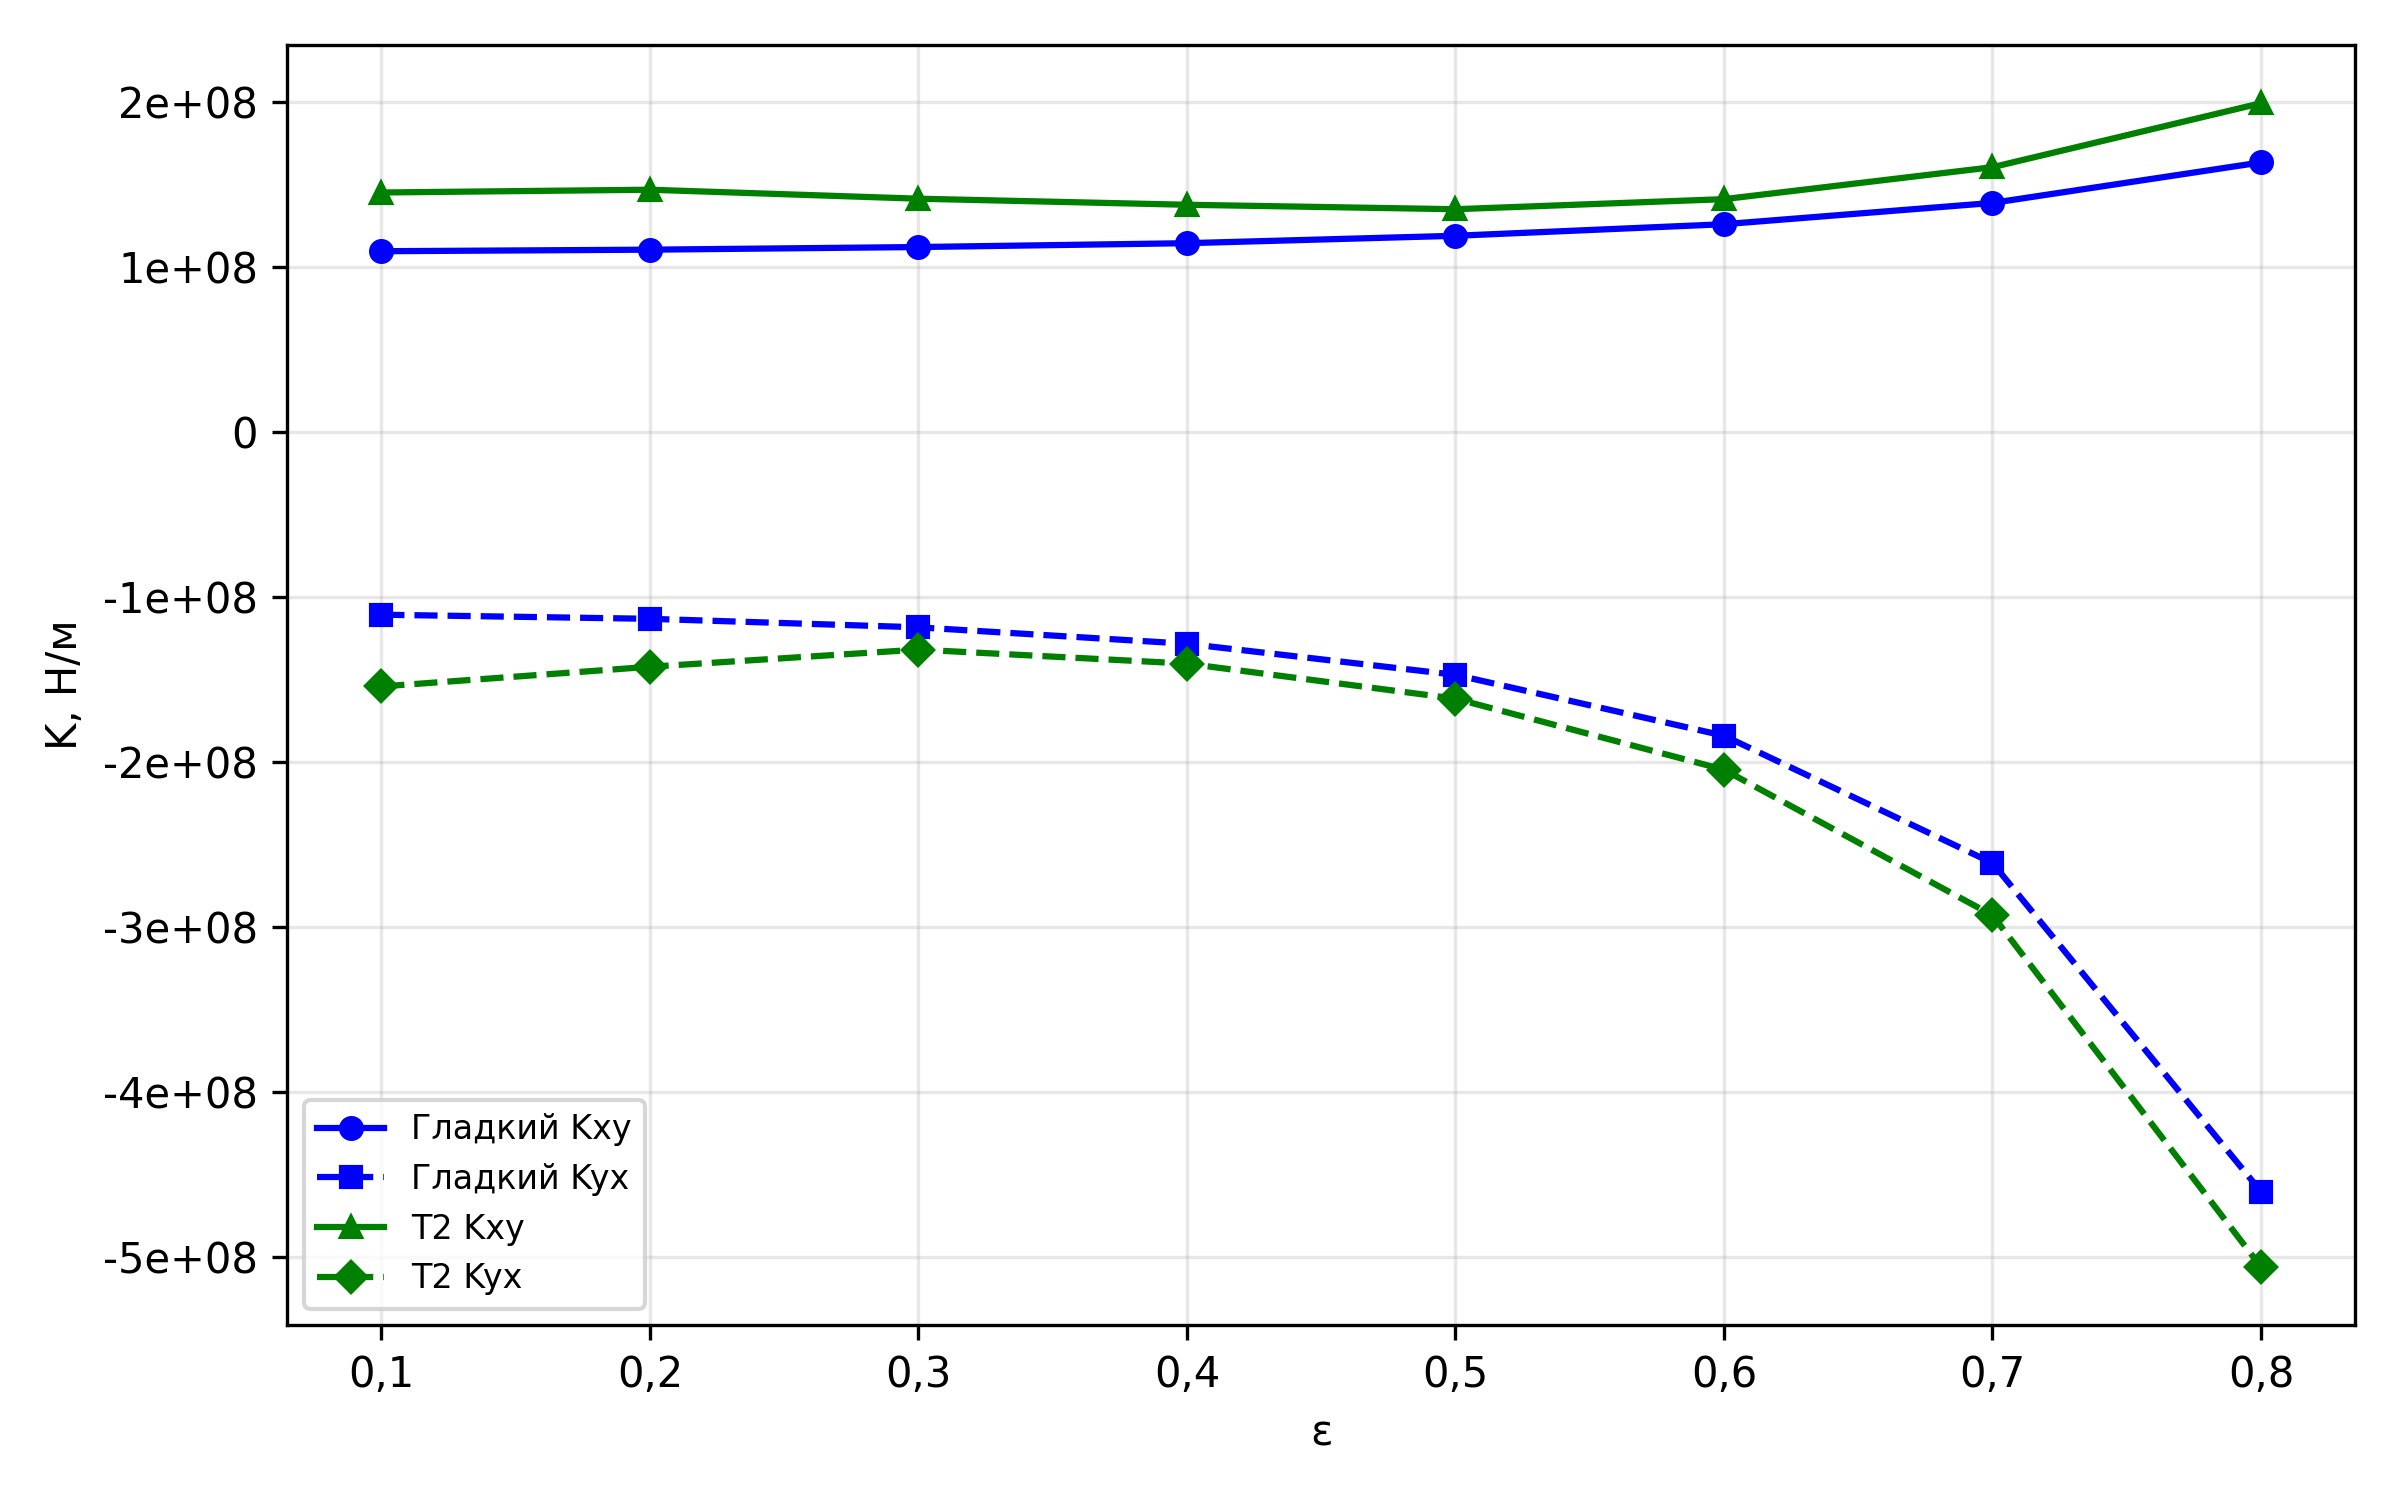
\includegraphics[width=\textwidth,height=0.9\textheight,keepaspectratio]{figures/ch08/fig_8_2.png}
\caption{Зависимость перекрёстных коэффициентов жёсткости $K_{xy}$
  и $K_{yx}$ от эксцентриситета~$\varepsilon$.}
\label{fig:dyn_K_cross}
\end{figure}


\section{Влияние эксцентриситета на коэффициенты демпфирования}

Прямые коэффициенты демпфирования $C_{xx}$ и $C_{yy}$ монотонно
возрастают с ростом~$\varepsilon$
(рисунок~\ref{fig:dyn_C_direct}). Конфигурация~T2 демонстрирует
несколько меньшие значения $C_{xx}$ и $C_{yy}$ по сравнению
с гладким подшипником. При $\varepsilon = 0{,}6$:
$C_{xx}^{(T2)} = 1{,}85 \cdot 10^6$~Н$\cdot$с/м против
$C_{xx}^{(\text{гл.})} = 2{,}57 \cdot 10^6$~Н$\cdot$с/м.

Перекрёстные коэффициенты демпфирования $C_{xy}$, $C_{yx}$
получены как предварительные оценки. Вследствие повышенной
чувствительности к шагу $\Delta v$ они не используются в данной
работе в качестве основных количественных показателей и не
включены в сравнительные таблицы.

\begin{figure}[!ht]
\centering
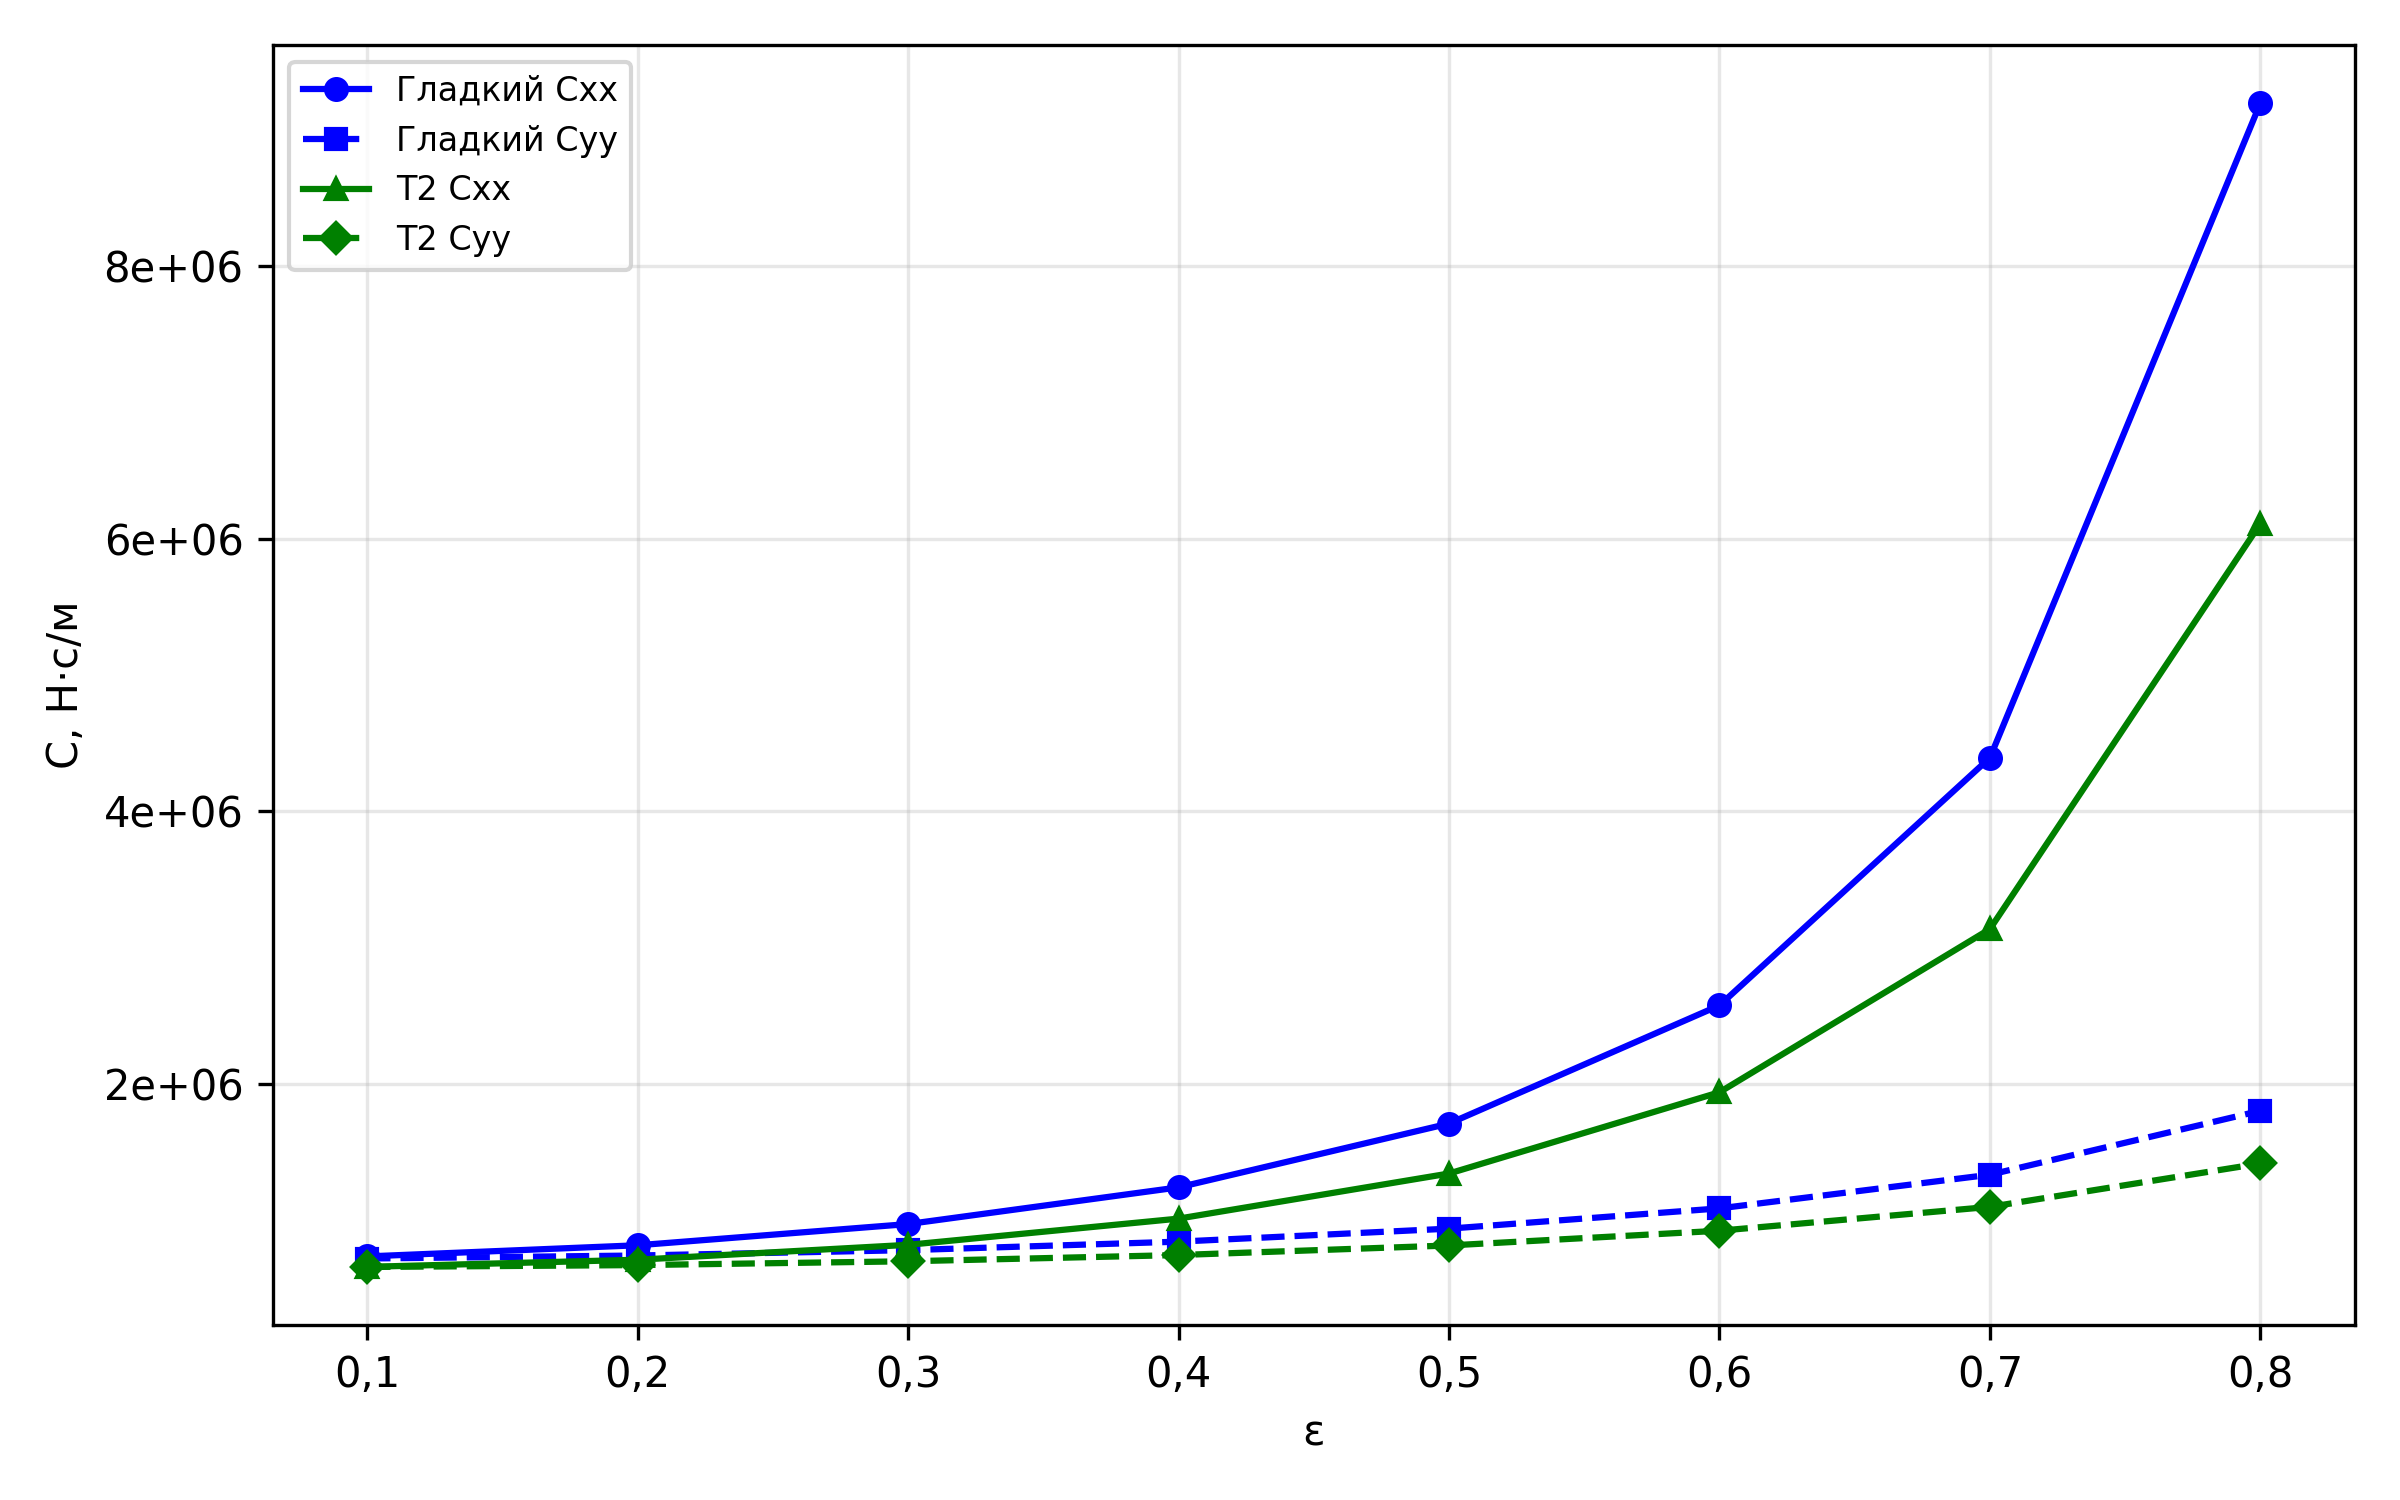
\includegraphics[width=\textwidth,height=0.9\textheight,keepaspectratio]{figures/ch08/fig_8_3.png}
\caption{Зависимость прямых коэффициентов демпфирования $C_{xx}$
  и $C_{yy}$ от эксцентриситета~$\varepsilon$
  для гладкого подшипника и конфигурации~T2.}
\label{fig:dyn_C_direct}
\end{figure}

\begin{figure}[!ht]
\centering
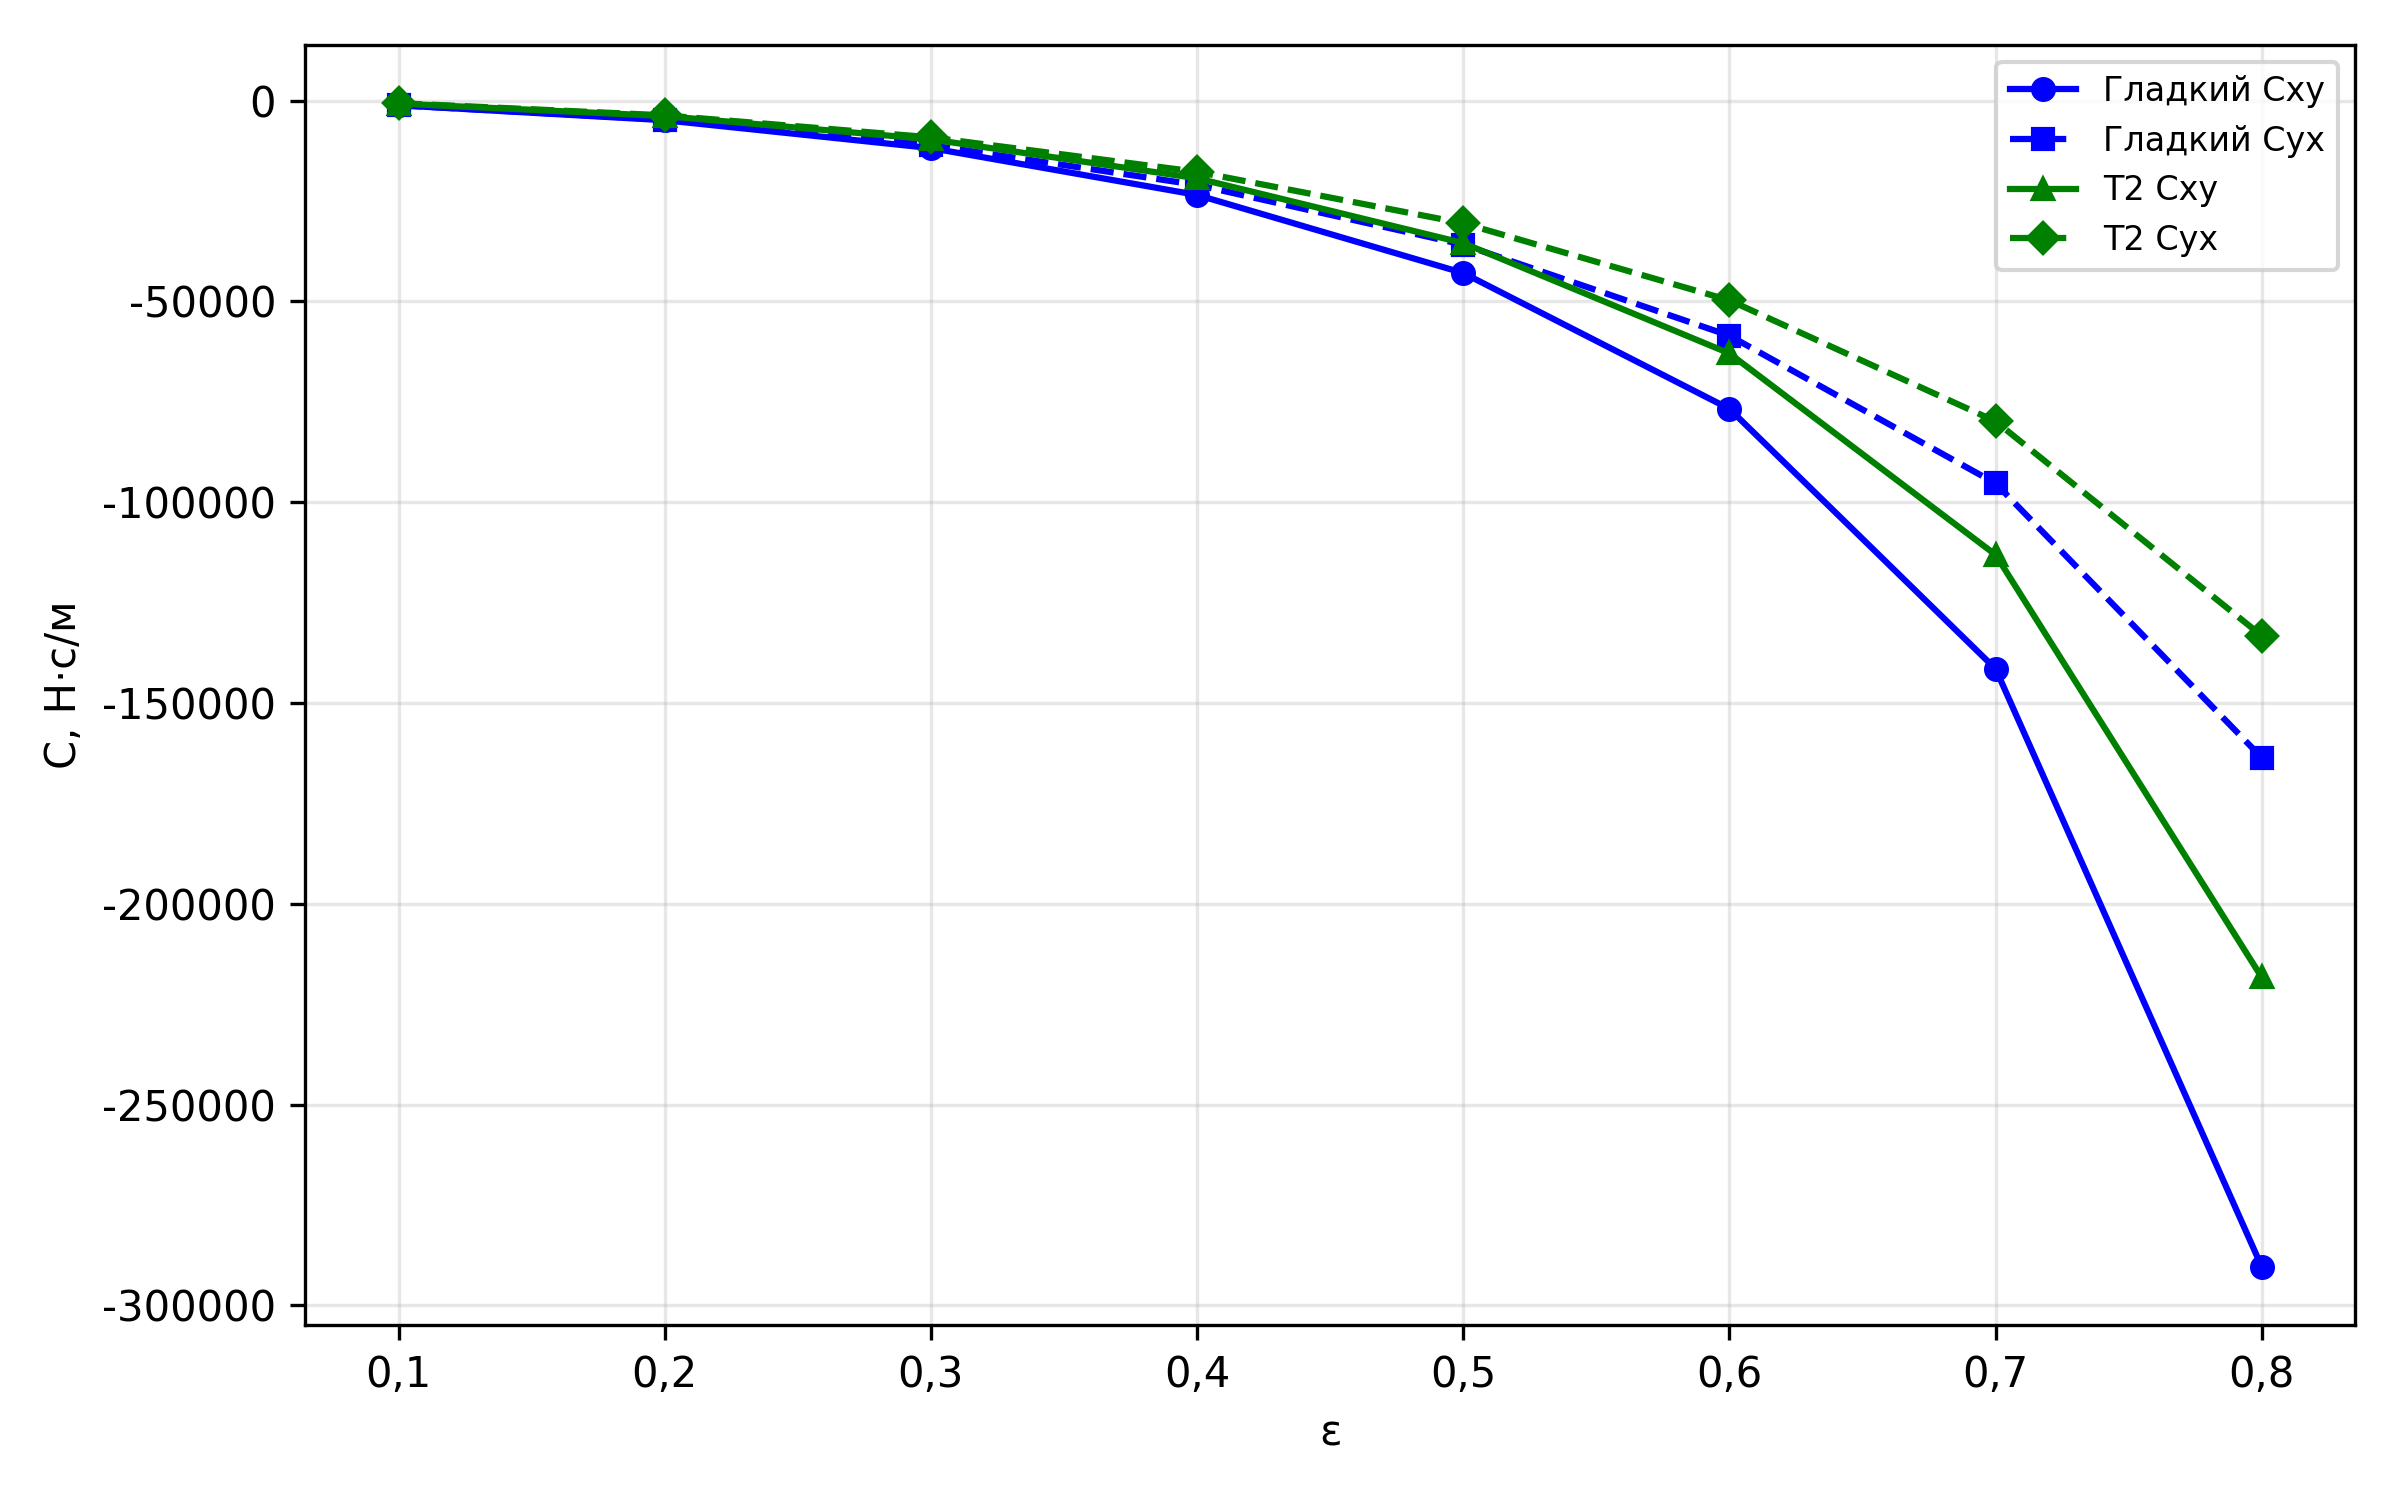
\includegraphics[width=\textwidth,height=0.9\textheight,keepaspectratio]{figures/ch08/fig_8_3a.png}
\caption{Зависимость перекрёстных коэффициентов демпфирования $C_{xy}$
  и $C_{yx}$ от эксцентриситета~$\varepsilon$.}
\label{fig:dyn_C_cross}
\end{figure}

\FloatBarrier


\section{Устойчивость и динамический отклик ротора}

\textit{Устойчивость.}
Во всём исследованном диапазоне
$\varepsilon = 0{,}2$--$0{,}6$ максимальная вещественная часть
собственных значений матрицы состояния
$\mathrm{Re}(\lambda_{\max}) < 0$ для обоих вариантов~--
система линейно устойчива
(рисунок~\ref{fig:dyn_Re_max}). С ростом~$\varepsilon$
значение $\mathrm{Re}(\lambda_{\max})$ становится более
отрицательным, то есть запас устойчивости увеличивается.

Конфигурация~T2 даёт существенно более отрицательные значения
$\mathrm{Re}(\lambda_{\max})$ по сравнению с гладким
подшипником. При $\varepsilon = 0{,}6$:
$\mathrm{Re}(\lambda_{\max})^{(T2)} = -282{,}5$ против
$-122{,}3$ у гладкого. Таким образом, конфигурация~T2 обеспечивает существенно более
высокий запас линейной устойчивости по сравнению с гладким
подшипником.

\begin{figure}[!ht]
\centering
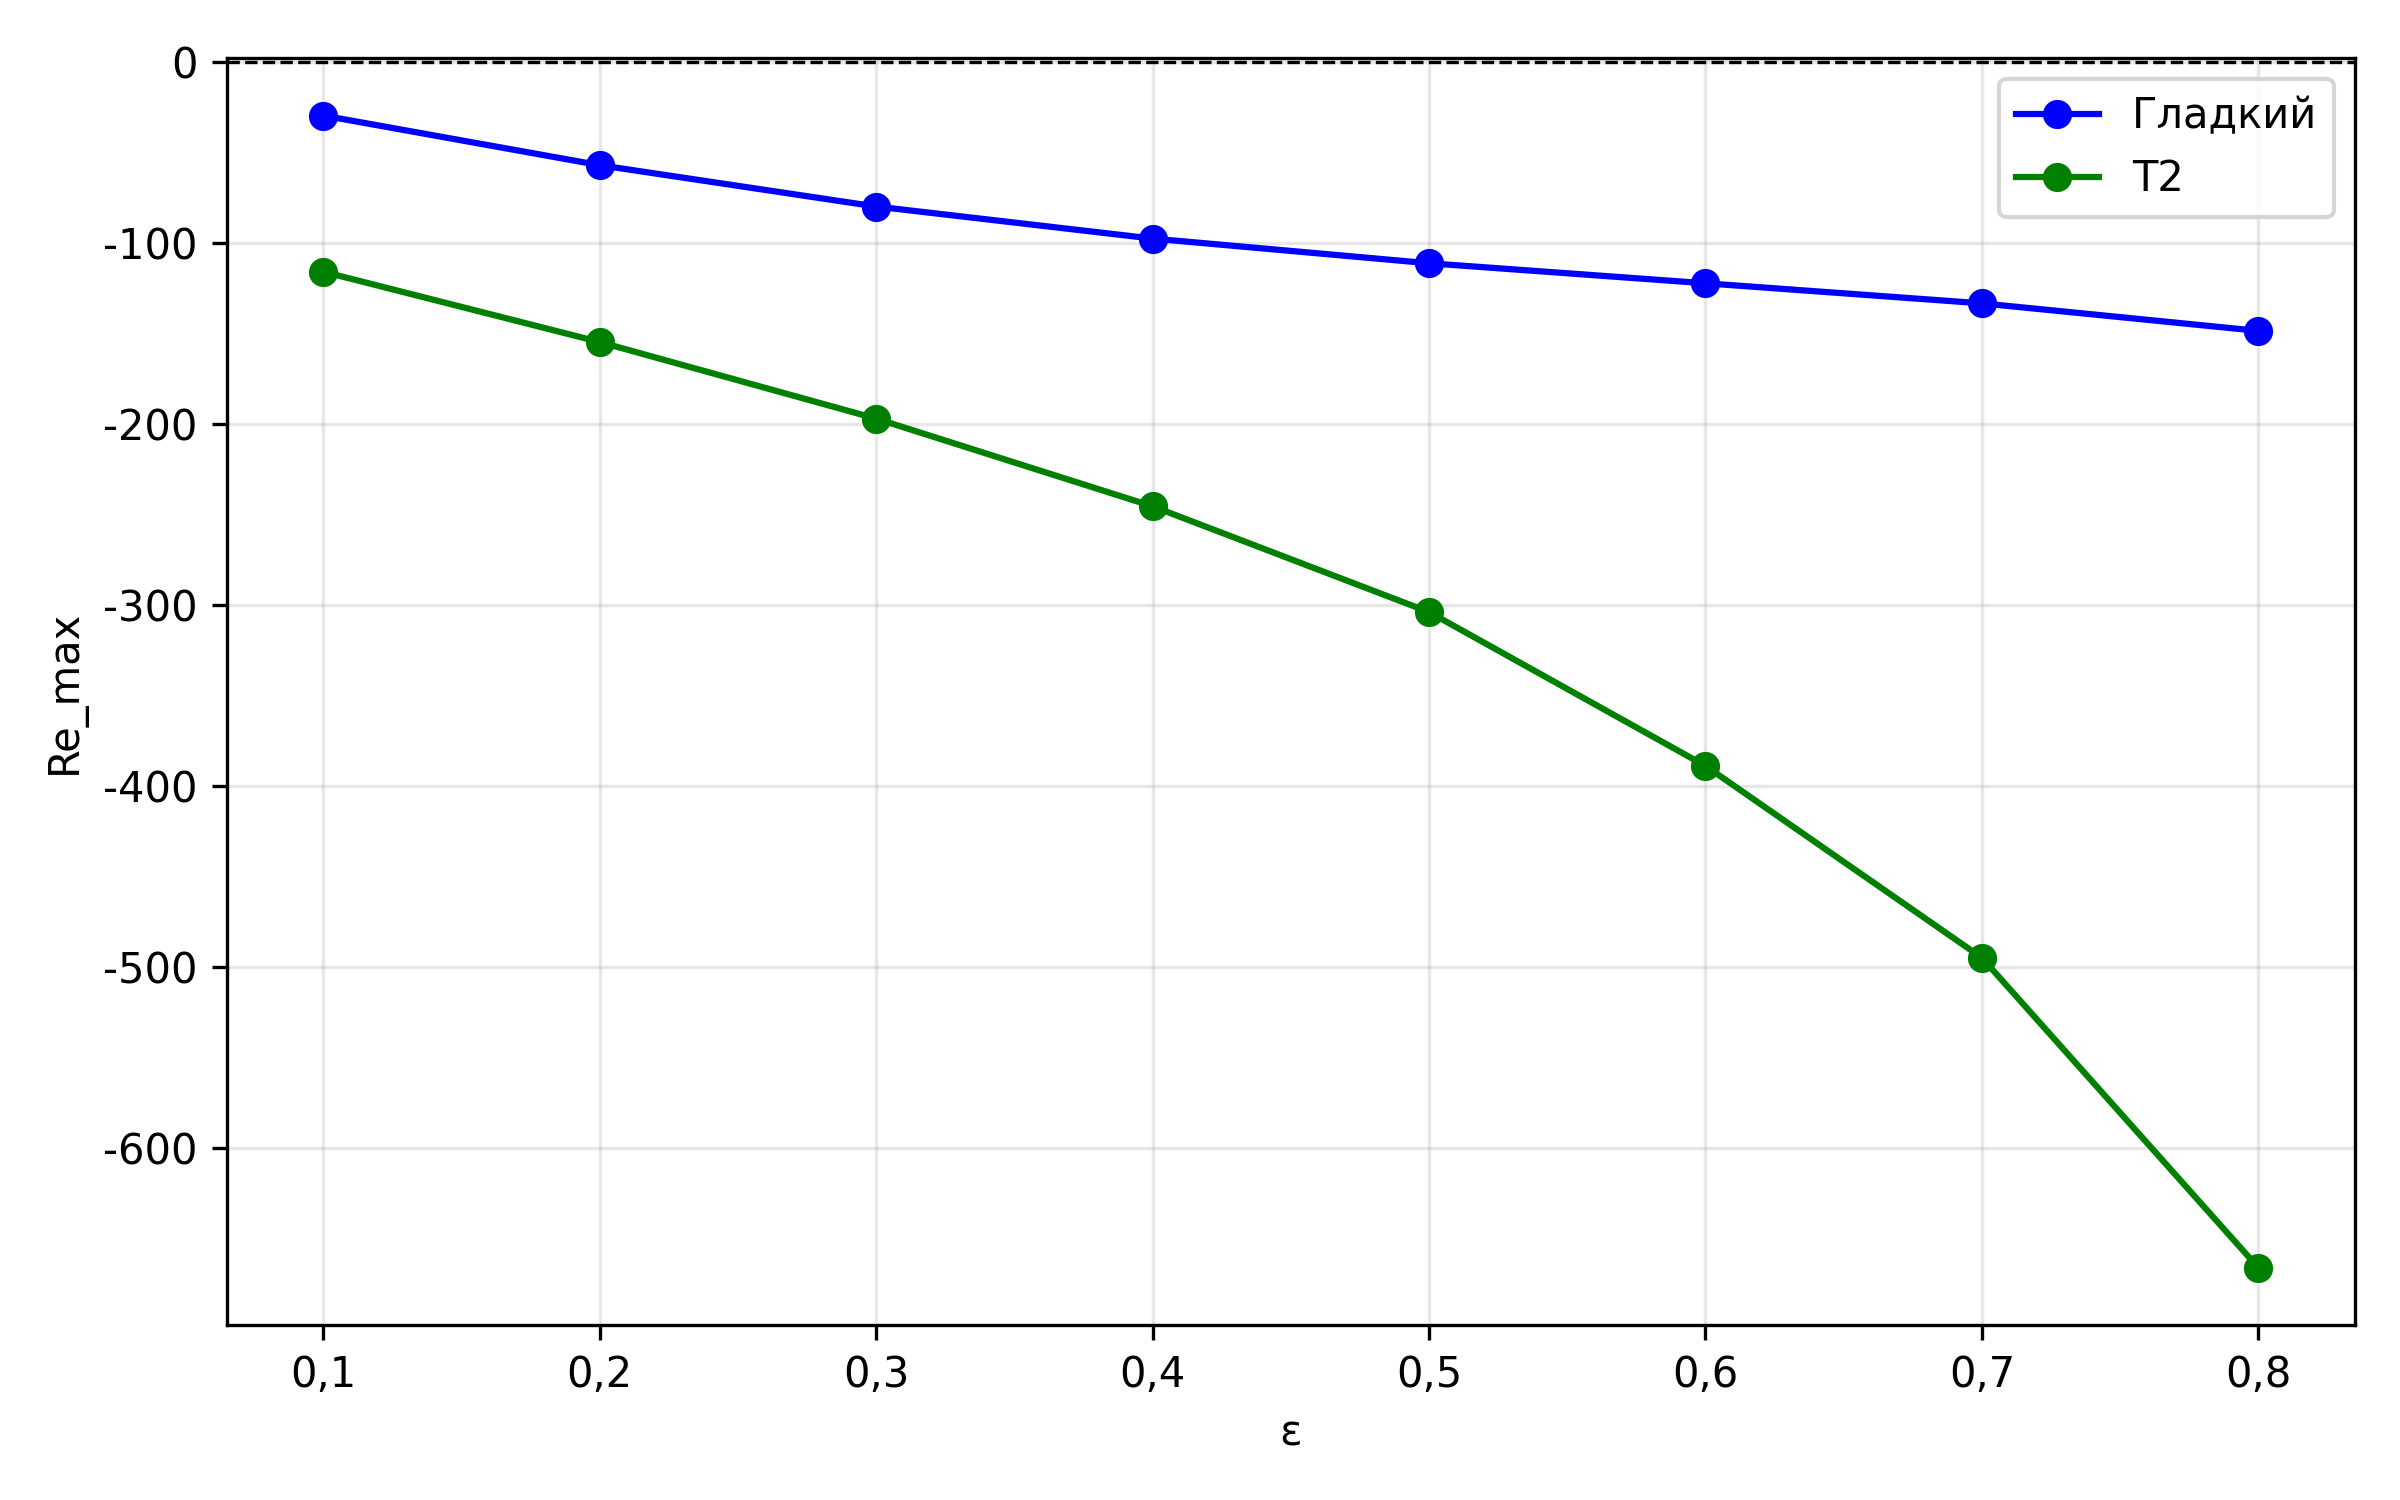
\includegraphics[width=\textwidth,height=0.9\textheight,keepaspectratio]{figures/ch08/fig_8_4.png}
\caption{Зависимость максимальной вещественной части собственных
  значений $\mathrm{Re}(\lambda_{\max})$ от
  эксцентриситета~$\varepsilon$. Пунктирная горизонталь
  $\mathrm{Re} = 0$~-- граница устойчивости.}
\label{fig:dyn_Re_max}
\end{figure}

\FloatBarrier

\textit{Динамический отклик ротора.}
Для $\varepsilon = 0{,}6$ выполнено численное интегрирование
линейной системы~\eqref{eq:dyn_ode_x}--\eqref{eq:dyn_ode_y}
в течение 20~оборотов при начальном возмущении
$\xi_0 = 0{,}01c$. Полная траектория центра цапфы
восстанавливается как $x_{\mathrm{tot}} = x_0 + \xi$,
$y_{\mathrm{tot}} = y_0 + \eta$.

Для гладкого подшипника: $\max|\xi| = 0{,}50$~мкм,
$\max|\eta| = 0{,}22$~мкм. Для~T2: $\max|\xi| = 0{,}50$~мкм,
$\max|\eta| = 0{,}11$~мкм. Максимальные отклонения значительно меньше
радиального зазора $c = 50$~мкм, что подтверждает применимость
линейного приближения. Конфигурация~T2 вдвое уменьшает
поперечную составляющую движения ротора. Временны\'{е} зависимости координат показаны на рис.~\ref{fig:dyn_orbit_time}, а траектории в плоскости $(x, y)$ -- на рис.~\ref{fig:dyn_orbit_xy}.

\begin{figure}[!ht]
\centering
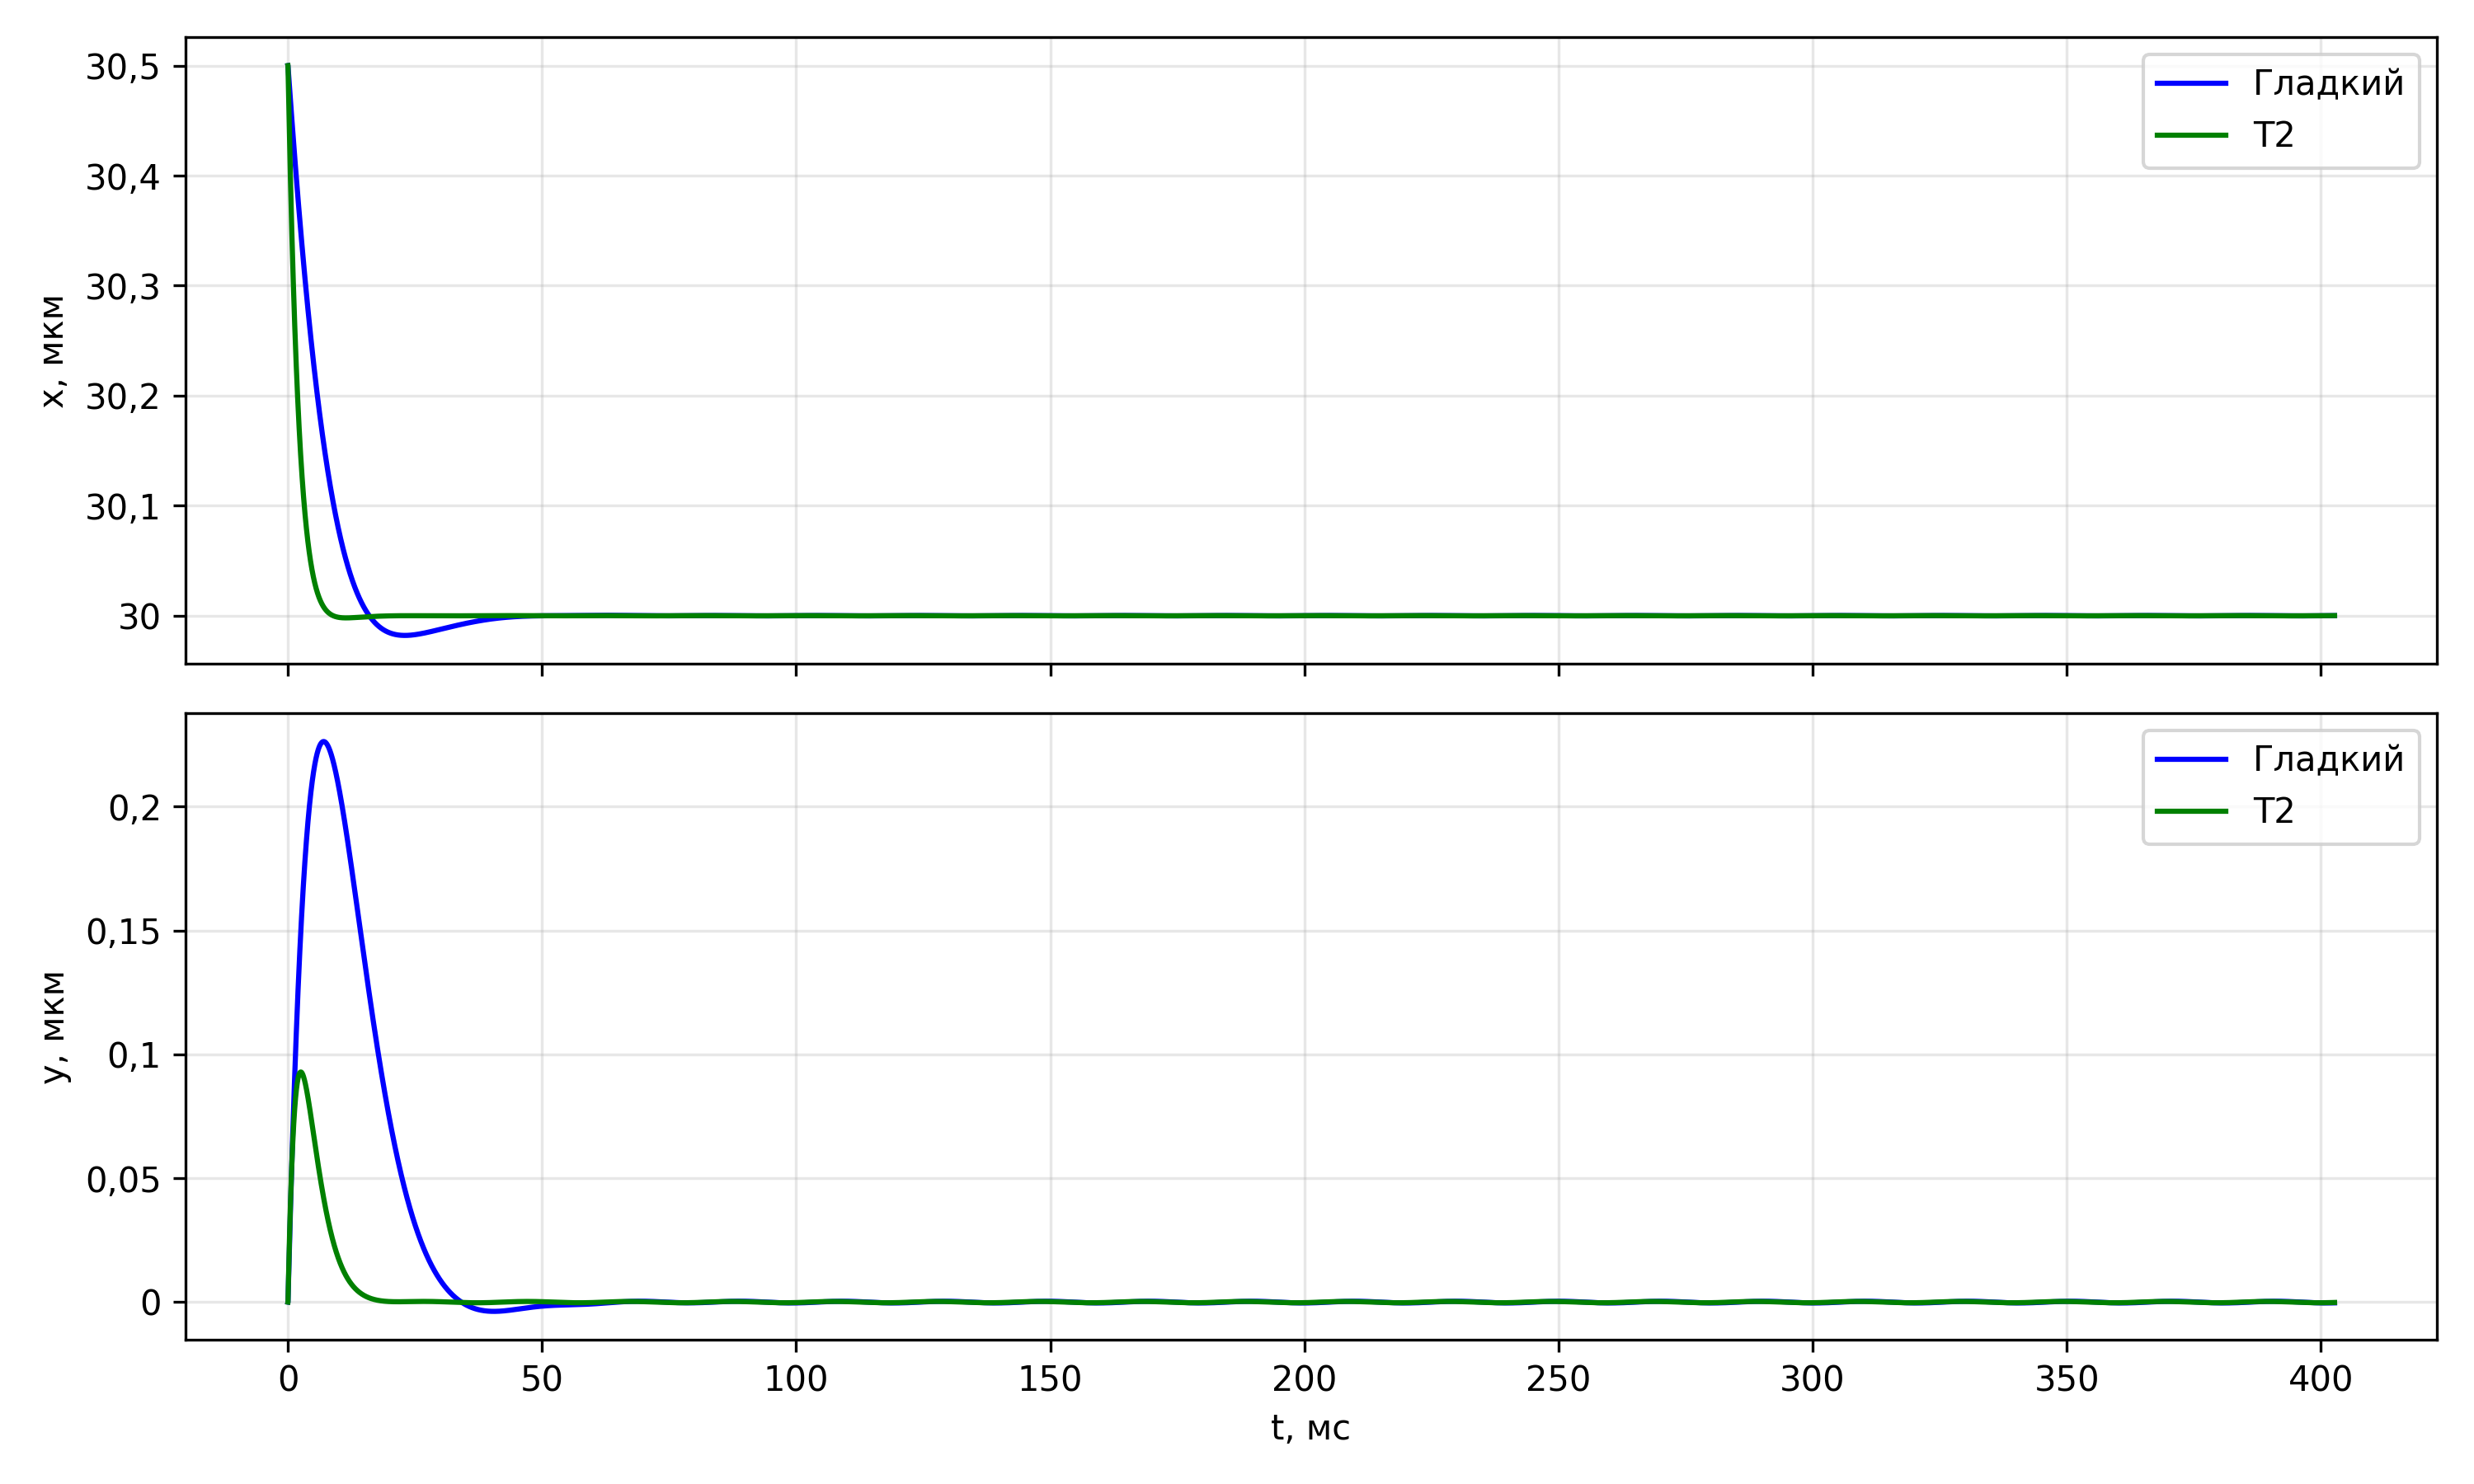
\includegraphics[width=\textwidth,height=0.9\textheight,keepaspectratio]{figures/ch08/fig_8_5.png}
\caption{Временны\'{е} зависимости координат центра цапфы
  $x_{\mathrm{tot}}(t)$ и $y_{\mathrm{tot}}(t)$
  при $\varepsilon = 0{,}6$ для гладкого подшипника
  и конфигурации~T2.}
\label{fig:dyn_orbit_time}
\end{figure}

\begin{figure}[!ht]
\centering
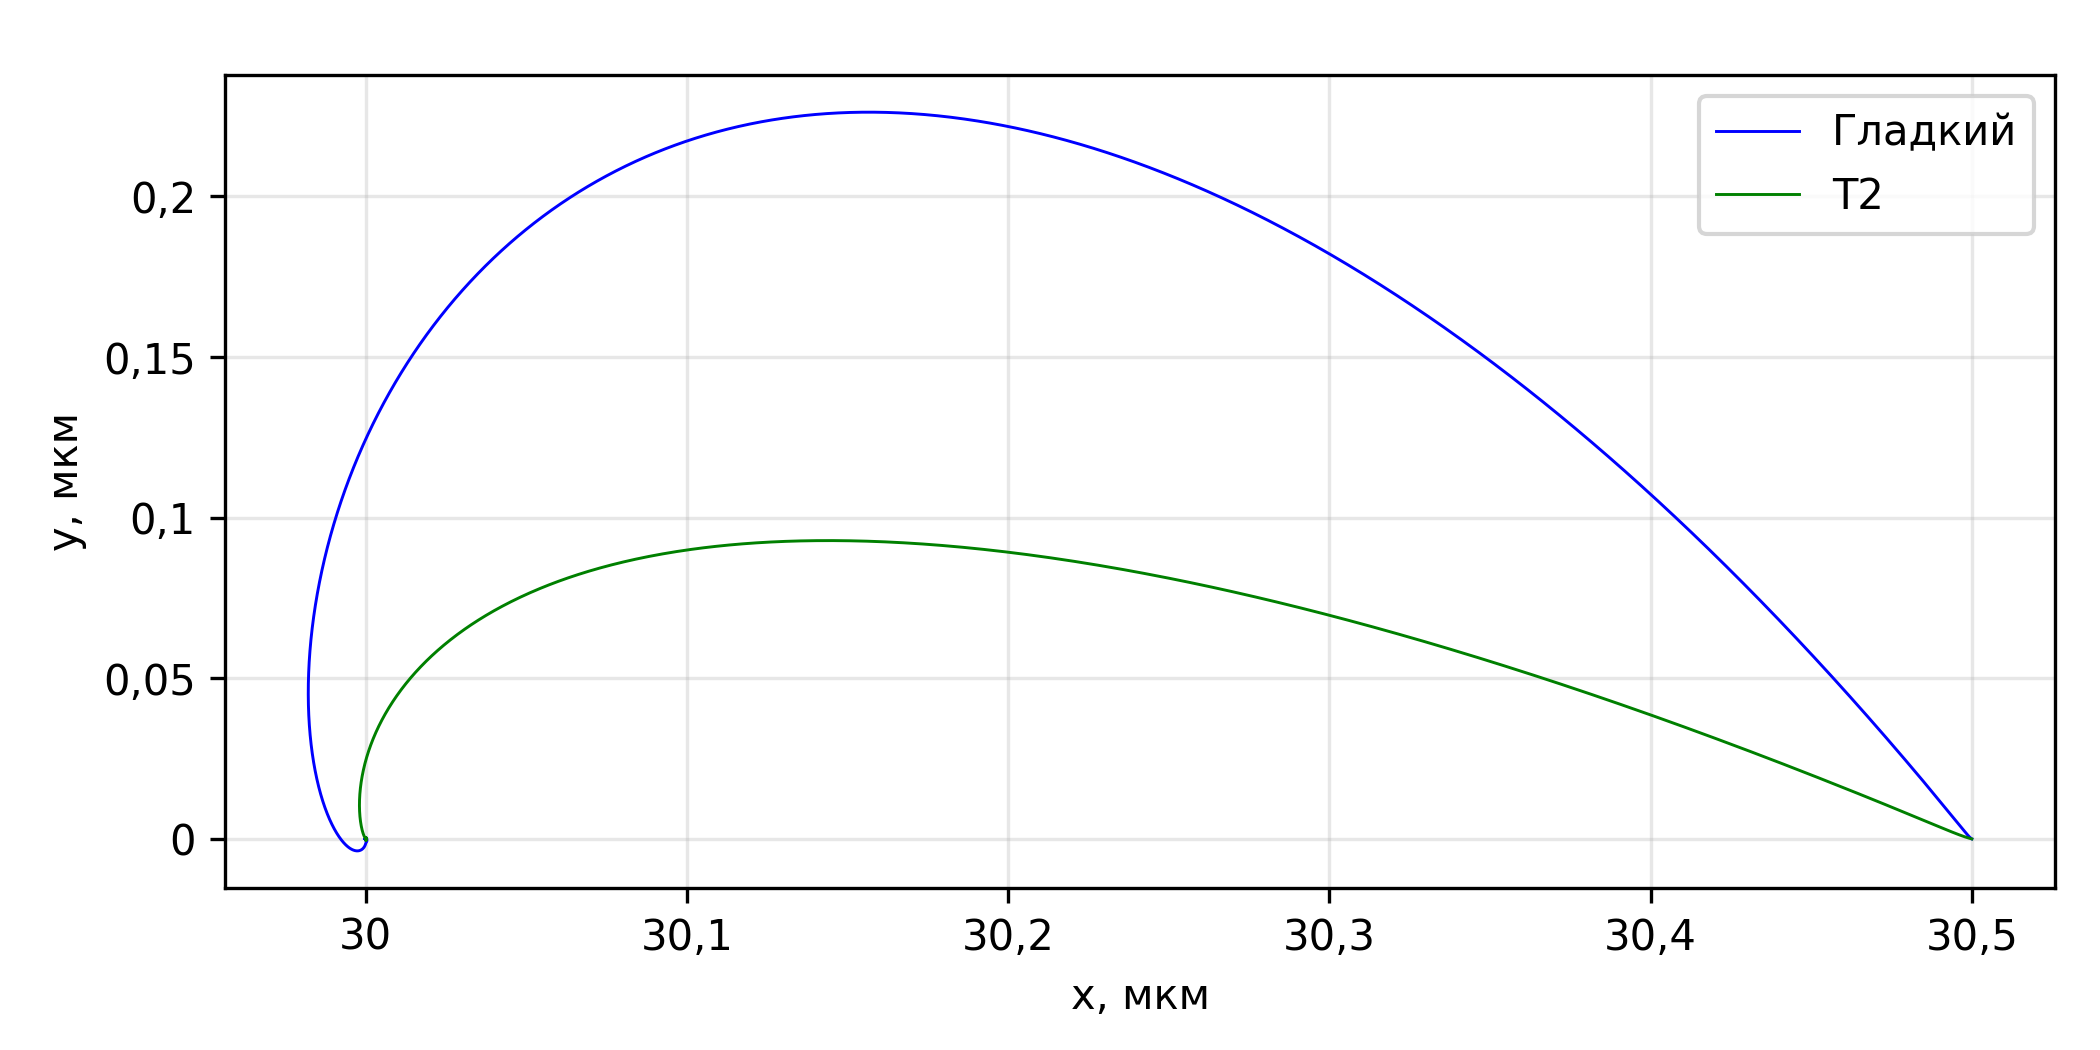
\includegraphics[width=\textwidth,height=0.9\textheight,keepaspectratio]{figures/ch08/fig_8_6.png}
\caption{Траектория центра цапфы в плоскости
  $(x_{\mathrm{tot}},\, y_{\mathrm{tot}})$
  при $\varepsilon = 0{,}6$ для гладкого подшипника
  и конфигурации~T2.}
\label{fig:dyn_orbit_xy}
\end{figure}

\FloatBarrier
\section*{Выводы по главе~8}
\phantomsection\addcontentsline{toc}{section}{Выводы по главе~8}

Разработана линейная динамическая модель системы «ротор~--
подшипник скольжения с микроструктурированной поверхностью»~\cite{han2022,conti2016,cui2018,bashmur2024a,bashmur2024b}.
Модель основана на статическом и динамическом уравнениях
Рейнольдса; динамический член выводится из единой функции
зазора~\eqref{eq:dyn_h} без дополнительных корректирующих
слагаемых. Коэффициенты жёсткости и демпфирования вычислены
методом центральных конечных разностей вокруг одной рабочей
точки.

Проведён сравнительный анализ гладкого подшипника
и конфигурации~T2 в диапазоне
$\varepsilon = 0{,}2$--$0{,}6$. Установлено, что текстура~T2
существенно увеличивает прямые коэффициенты динамической
жёсткости: при $\varepsilon = 0{,}6$ значение $K_{xx}$
возрастает на~$78\,\%$.

Анализ линейной устойчивости по знаку
$\mathrm{Re}(\lambda_{\max})$ показал, что оба варианта
устойчивы во всём исследованном диапазоне эксцентриситетов.
Конфигурация~T2 обеспечивает существенно более высокий запас
линейной устойчивости по сравнению с гладким подшипником.

При $\varepsilon = 0{,}6$ текстурированный вариант примерно вдвое уменьшает максимальное отклонение ротора
по оси~$y$ ($\max|\eta|$:
с $0{,}22$~мкм до $0{,}11$~мкм). Максимальные отклонения ротора значительно
меньше радиального зазора, что подтверждает применимость
линейного приближения.

Перекрёстные коэффициенты демпфирования $C_{xy}$, $C_{yx}$
проявили повышенную чувствительность к шагу численного
дифференцирования и не используются как окончательные
количественные результаты. Верификация прямых жёсткостей
и демпфирований подтвердила их численную устойчивость
при изменении шага и сетки.

Полученные результаты дополняют выводы главы~5 о статических
преимуществах текстурирования, показывая, что применение
детерминированных микроструктур улучшает также динамические
характеристики радиального подшипника скольжения.
              % УБРАНО из учебника

% --- Заключение ---
% ============================================================
% Заключение
% ============================================================
\chapter*{Заключение}
\phantomsection\addcontentsline{toc}{chapter}{Заключение}

В~настоящем учебном пособии систематизированы теоретические основы и~методы анализа дискретного микрорельефа рабочей поверхности деталей машин применительно к~подшипникам скольжения.

В~первой главе рассмотрены общие сведения о~подшипниках скольжения: классификация, принцип работы гидродинамического подшипника, режимы трения, конструкции и~области применения. Систематизированы виды детерминированных микроструктур рабочей поверхности, включая их~типы, формы, параметры, схемы расположения и~технологии формирования. Показано, что влияние микроструктур на~трибологические характеристики обусловлено генерацией дополнительного гидродинамического давления, удержанием смазки при~пусковых режимах и~захватом частиц износа. Рассмотрена связь поверхностного текстурирования с~концепцией зелёной трибологии.

Во~второй главе сформулирована единая математическая основа для~численного моделирования смазочного слоя. Для~трёх типовых постановок (радиальный подшипник, упорный подшипник, обратная пара) введены согласованные поверхностные координаты, масштабы безразмеризации и~унифицированная форма уравнения Рейнольдса. Сформулирована параметрическая модель микрорельефа и~массосохраняющая постановка кавитации (JFO).

В~третьей главе описана численная реализация решения задач гидродинамики смазочного слоя: консервативная дискретизация, метод Red-Black SOR на~GPU, алгоритм решения задачи кавитации JFO с~двухуровневой итерационной структурой.

В~четвёртой главе проанализировано влияние дополнительных эффектов на~характеристики смазочного слоя: нелинейность (пьезовязкость и~сжимаемость), термовязкостные эффекты и~шероховатость поверхности. Сформулирована иерархия моделей-расширений базовой изотермической постановки.

В~пятой главе приведены три~подробных примера инженерного расчёта подшипников скольжения с~микрорельефом: радиальный подшипник центробежного насоса, радиальный подшипник шарошечного долота и~упорный подшипник с~секторными колодками. Каждый пример демонстрирует полный цикл расчёта~-- от~постановки задачи и~выбора параметров микроструктур до~анализа и~интерпретации результатов. Показано, что оптимально подобранные микроструктуры способны существенно повысить несущую способность подшипника и~снизить потери на~трение.

\textbf{Практическое значение.} Полученные знания и~навыки могут быть использованы при~проектировании и~модернизации подшипниковых узлов технологических машин и~оборудования нефтегазовой, энергетической и~других отраслей. Методика расчёта, освоенная при~выполнении курсовой работы, позволяет обучающемуся самостоятельно оценивать эффективность применения микрорельефа для~конкретных условий эксплуатации.

\textbf{Перспективы развития.} Направление анализа и~оптимизации микрорельефа рабочих поверхностей продолжает активно развиваться. К~перспективным задачам относятся: учёт термогидродинамических эффектов в~расчётах текстурированных подшипников, многокритериальная оптимизация параметров микроструктур с~применением методов машинного обучения, разработка новых технологий формирования микрорельефа (аддитивные технологии, ультракороткоимпульсная лазерная обработка), а~также расширение области применения текстурирования на~другие узлы трения~-- уплотнения, направляющие, зубчатые передачи.


% --- Список использованных источников ---
% =============================================================
% Список использованных источников
% п. 6.9, п. 7.10: оформление по ГОСТ Р 7.0.100, ГОСТ 7.80
% =============================================================
\chapter*{Список использованных источников}
\phantomsection\addcontentsline{toc}{chapter}{Список использованных источников}
\printbibliography[heading=none]


\end{document}
